% =====================================================================
%  دليل أدوات البناء — الملف الرئيسي (HTML فقط)
%  دليل مستقل يفتحه الفصل 6 من الدليل الرئيسي، وفصوله مرقمة من 1.
%  يُبنى إلى site/<lang>/builder.html و b1.html … في المجلد نفسه.
%  لإضافة فصل: أنشئ builder/chapters/NN-name.tex وأضف سطر \input له هنا،
%  ثم أضف الملف نفسه في i18n/en/builder/.
% =====================================================================
\documentclass[11pt,oneside,openany]{report}
% =====================================================================
%  preamble.tex — shared design settings for the KayanOS guide
%  Visual reference: «نموذج رايت كود - Copy.docx» (RightCode template)
%  Build with XeLaTeX. Content lives in chapters/; never put design here
%  into chapter files.
% =====================================================================

% ---------- Page geometry (from the template body section) ----------
% Body: A4, top/bottom 1247tw = 2.2cm, sides 1020tw = 1.8cm,
% header/footer distance 567tw = 1.0cm.
\usepackage[a4paper,top=2.6cm,bottom=2.4cm,left=1.8cm,right=1.8cm,
            headsep=0.5cm,footskip=1.0cm,headheight=1.0cm]{geometry}

% ---------- Packages (order matters: polyglossia/bidi load last) ----------
\usepackage{fontspec}
\usepackage[table]{xcolor}
\usepackage{graphicx}
\usepackage{tikz}
\usetikzlibrary{arrows.meta,positioning,calc,fit,backgrounds,shapes.geometric}
\usepackage{array,booktabs,tabularx,longtable}
\usepackage{enumitem}
\usepackage{fancyhdr}
\usepackage{titlesec}
\usepackage[most]{tcolorbox}
\usepackage{caption}
\usepackage{float} % [H] keeps a figure next to the text that explains it
\usepackage{eso-pic}
\usepackage{lastpage}
\usepackage[hidelinks]{hyperref}
\usepackage{polyglossia}

% ---------- Brand colors (template + RightCode brand tokens) ----------
\definecolor{rcPrimary}{HTML}{00696D}      % Heading 2 / accent teal
\definecolor{rcPrimaryLight}{HTML}{4FB8AE} % cover kicker
\definecolor{rcDark}{HTML}{052424}         % cover background
\definecolor{rcText}{HTML}{0E1F1F}         % Normal text
\definecolor{rcTextSecondary}{HTML}{4A6364}% Heading 5
\definecolor{rcMuted}{HTML}{94A8A6}        % caption, header, footer
\definecolor{rcMutedDark}{HTML}{6A8482}    % cover meta labels
\definecolor{rcSurfaceVar}{HTML}{E5EBEB}   % cover meta values
\definecolor{rcSurfaceElev}{HTML}{F1F5F4}  % zebra rows / boxes
\definecolor{rcBorder}{HTML}{D6E0DF}       % hairlines
\definecolor{rcSuccess}{HTML}{1E7F4D}\definecolor{rcSuccessBg}{HTML}{E3F4EB}
\definecolor{rcWarning}{HTML}{A36300}\definecolor{rcWarningBg}{HTML}{FBF1DD}
\definecolor{rcError}{HTML}{B23131}  \definecolor{rcErrorBg}{HTML}{F8E3E3}
\definecolor{rcInfo}{HTML}{1E5C7F}   \definecolor{rcInfoBg}{HTML}{E1EEF6}

% ---------- Languages and fonts ----------
\setdefaultlanguage[numerals=maghrib]{arabic} % Western digits 0-9
\setotherlanguage{english}
\gappto\captionsarabic{\renewcommand{\chaptername}{الفصل}}

\defaultfontfeatures{Path=fonts/,Extension=.ttf}
% Arabic is the main font: Noto Naskh Arabic (template Normal style cs font).
% Arabic has no italic; italic falls back to regular.
\setmainfont{NotoNaskhArabic}[Script=Arabic,
  UprightFont=*-Regular,BoldFont=*-Bold,ItalicFont=*-Regular,
  BoldItalicFont=*-Bold]
\newfontfamily\arabicfont{NotoNaskhArabic}[Script=Arabic,
  UprightFont=*-Regular,BoldFont=*-Bold,ItalicFont=*-Regular,
  BoldItalicFont=*-Bold]
\newfontfamily\arabicfontsf{NotoNaskhArabic}[Script=Arabic,
  UprightFont=*-Regular,BoldFont=*-Bold]
\newfontfamily\arabicfonttt{NotoNaskhArabic}[Script=Arabic,
  UprightFont=*-Regular,BoldFont=*-Bold]
% Latin: Lora (template Normal style ascii/hAnsi font) — use \en{...}
\newfontfamily\englishfont{Lora}[UprightFont=*-Regular,BoldFont=*-Bold,
  ItalicFont=*-Italic,BoldItalicFont=*-BoldItalic]

% Body: 11pt, line 1.15 (template docDefaults line=276), text color
\linespread{1.15}
\color{rcText}
\setlength{\parindent}{0pt}
\setlength{\parskip}{4pt} % template Normal spacing after = 80tw

% Latin terms inside Arabic text
\newcommand{\en}[1]{\textenglish{#1}}
\newcommand{\kos}{\en{KayanOS}}
% Technical key (first appearance only)
% (\textcolor, not \color: under bidi a bare \color leaks into later paragraphs)
\newcommand{\key}[1]{{\textenglish{\small\textcolor{rcPrimary}{#1}}}}

% ---------- Headings (template Heading 1/2/3) ----------
% Heading 1: bold 24pt, text color. Heading 2: bold 18pt teal.
% Heading 3: bold 14pt. Caption: italic 9pt muted.
\titleformat{\chapter}[display]
  {\bfseries\color{rcText}}
  {\color{rcPrimaryLight}\large\chaptertitlename\ \thechapter}
  {2pt}{\fontsize{24}{32}\selectfont}
  [\vspace{4pt}{\color{rcPrimary}\rule{3cm}{1.2pt}}]
\titlespacing*{\chapter}{0pt}{0pt}{18pt}
\titleformat{\section}{\bfseries\fontsize{18}{26}\selectfont\color{rcPrimary}}
  {\thesection}{0.6em}{}
\titlespacing*{\section}{0pt}{14pt}{6pt}
\titleformat{\subsection}{\bfseries\fontsize{14}{20}\selectfont\color{rcText}}
  {\thesubsection}{0.6em}{}
\titlespacing*{\subsection}{0pt}{10pt}{3pt}
\titleformat{\subsubsection}{\bfseries\color{rcPrimary}}{}{0pt}{}

\captionsetup{font={small,it,color=rcMuted},labelfont={bf,color=rcMuted},
  labelsep=colon,skip=6pt}

% ---------- Header & footer (template header3 / footer1) ----------
\newcommand{\guideTitle}{دليل \kos}
\newcommand{\guideBrand}{\en{RightCode}\ \ ·\ \ \guideTitle\ \ ·\ \ \en{rightcode.io}}

\fancypagestyle{rcbody}{%
  \fancyhf{}%
  \renewcommand{\headrulewidth}{0pt}%
  \renewcommand{\footrulewidth}{0pt}%
  \fancyhead[R]{{\footnotesize\color{rcText}\guideTitle}\\[-2pt]
                {\scriptsize\color{rcMuted}\leftmark}}%
  \fancyhead[L]{
\includegraphics[width=3.11cm,height=0.8cm]{assets/logo.png}}%
  \fancyfoot[R]{\scriptsize\color{rcMuted}\guideBrand}%
  \fancyfoot[L]{\scriptsize\color{rcMuted}\en{\thepage\ / \pageref{LastPage}}}%
}
\fancypagestyle{plain}{\pagestyle{rcbody}} % chapter opening pages too
\renewcommand{\chaptermark}[1]{\markboth{#1}{}}

% Page watermark: template places image3 behind body text at 40% opacity
\newif\ifrcwatermark \rcwatermarktrue
\AddToShipoutPictureBG{%
  \ifrcwatermark
    \AtPageCenter{\makebox[0pt]{\raisebox{-0.5\height}{%
      % watermark-40.png = watermark.png pre-blended at 40% over white
      % (PDF transparency inside shipout is unreliable across viewers)
      
\includegraphics[width=18.67cm,height=26.4cm]{assets/watermark-40.png}}}}%
  \fi}

% ---------- Cover (template first section: dark full-bleed page) ----------
% Usage: \makecover{kicker}{title}{subtitle}{date}{version}{prepared by}
\newcommand{\makecover}[6]{%
  \pagenumbering{alph}% unique page anchors for the cover
  \begin{titlepage}
  \rcwatermarkfalse
  \thispagestyle{empty}
  \AddToShipoutPictureBG*{\AtPageCenter{\makebox[0pt]{\raisebox{-0.5\height}{%
    
\includegraphics[width=\paperwidth,height=\paperheight]{assets/cover-bg.png}}}}}
  \centering
  % template: top margin 7.2cm + 2.1cm before the kicker (page top = 2.6cm)
  \vspace*{6.4cm}
  {\bfseries\small\color{rcPrimaryLight}#1\par}
  \vspace{14pt}
  {\bfseries\fontsize{22}{36}\selectfont\color{white}#2\par}
  \vspace{8pt}
  {\bfseries\small\color{rcPrimaryLight}#3\par}
  \vspace{5.2cm}
  % Meta strip: 3 equal cells, label above value (template cover table).
  % Drawn with TikZ: table cells reset the text color under bidi.
  \begin{tikzpicture}[x=4.6cm]
    \foreach \i/\lbl/\val in {0/التاريخ/{#4},-1/الإصدار/{#5},-2/أُعدّ بواسطة/{#6}}{
      \node[font=\bfseries\fontsize{7.5}{10}\selectfont,text=rcMutedDark] at (\i,0.5) {\RL{\lbl}};
      \node[font=\fontsize{9.5}{12}\selectfont,text=rcSurfaceVar] at (\i,0) {\RL{\val}};
    }
  \end{tikzpicture}
  \vfill
  \end{titlepage}
  \pagenumbering{arabic}%
  \rcwatermarktrue}

% ---------- Tables (RightCode brand table style) ----------
% Teal header band, white bold labels, zebra rows, hairline borders.
\newcolumntype{R}[1]{>{\raggedleft\arraybackslash}p{#1}}
\newcolumntype{Y}{>{\raggedleft\arraybackslash}X}
\newcommand{\rcHeaderRow}{\rowcolor{rcPrimary}}
\newcommand{\thh}[1]{\textcolor{white}{\bfseries #1}}
\newcommand{\rcZebra}{\rowcolors{2}{white}{rcSurfaceElev}}
\arrayrulecolor{rcBorder}
\setlength{\arrayrulewidth}{0.4pt}
\renewcommand{\arraystretch}{1.35}

% Data-classification badges (used in every "Before you start" table)
\newcommand{\rcbadge}[2]{\tikz[baseline=(b.base)]\node[fill=#1,text=white,
  rounded corners=2pt,inner xsep=4pt,inner ysep=1.5pt,font=\scriptsize\bfseries](b){\RL{#2}};}
\newcommand{\req}{\rcbadge{rcPrimary}{إلزامي تقنياً}}
\newcommand{\rec}{\rcbadge{rcPrimaryLight}{موصى به}}
\newcommand{\opt}{\rcbadge{rcMuted}{اختياري}}
\newcommand{\gen}{\rcbadge{rcTextSecondary}{يولّده النظام}}

% ---------- Image explanation (printed directly under a figure) ----------
\newcommand{\shotnote}[1]{\par\vspace{2pt}{\small #1\par}}

% ---------- Checklists ----------
\newlist{checklist}{itemize}{2}
\newcommand{\rccheckbox}{\tikz[baseline=-0.25ex]\draw[rcPrimary,line width=0.9pt,
  rounded corners=1pt](0,-0.05)rectangle(0.3,0.25);}
\setlist[checklist]{label={\rccheckbox},
  leftmargin=*,itemsep=2pt,topsep=4pt}
\newtcolorbox{rcchecklist}[1][قائمة تحقق]{enhanced,breakable,
  colback=rcSurfaceElev,colframe=rcPrimary,boxrule=0pt,
  leftrule=0pt,rightrule=3pt,arc=2pt,
  fonttitle=\bfseries\color{rcPrimary},coltitle=rcPrimary,
  colbacktitle=rcSurfaceElev,title={#1},
  left=10pt,right=10pt,top=4pt,bottom=6pt}

% ---------- Callouts ----------
\newtcolorbox{rcnote}[1][ملاحظة]{enhanced,breakable,colback=rcInfoBg,
  colframe=rcInfo,boxrule=0pt,rightrule=3pt,arc=2pt,
  title={#1},fonttitle=\bfseries,coltitle=rcInfo,colbacktitle=rcInfoBg}
\newtcolorbox{rcwarn}[1][تنبيه]{enhanced,breakable,colback=rcWarningBg,
  colframe=rcWarning,boxrule=0pt,rightrule=3pt,arc=2pt,
  title={#1},fonttitle=\bfseries,coltitle=rcWarning,colbacktitle=rcWarningBg}

% ---------- Diagram conventions (fixed for the whole guide) ----------
% RULE: TikZ nodes are laid out left-to-right. Wrap every Arabic label in
% \RL{...} (one \RL per line in multi-line nodes), e.g. \node[entity]{\RL{المناصب}};
% Boxes:   solid teal = required entity/page, dashed = optional,
%          grey fill  = generated by the system.
% Arrows:  solid  "dependsOn"  A -> B  means "A requires B to exist first".
%          dashed "flowsTo"    A -> B  means "the process moves from A to B".
\tikzset{
  rc/.style={font=\small,align=center},
  entity/.style={rc,draw=rcPrimary,line width=0.9pt,fill=white,
    rounded corners=3pt,minimum width=2.6cm,minimum height=0.95cm},
  entityOpt/.style={entity,dashed,draw=rcPrimaryLight},
  entityGen/.style={entity,draw=rcMuted,fill=rcSurfaceElev,text=rcTextSecondary},
  stepBox/.style={rc,fill=rcPrimary,text=white,rounded corners=3pt,
    minimum width=2.6cm,minimum height=0.95cm,font=\small\bfseries},
  dependsOn/.style={-{Stealth[length=7pt]},line width=1pt,draw=rcPrimary},
  dependsOnOpt/.style={dependsOn,densely dotted,draw=rcPrimaryLight},
  flowsTo/.style={-{Latex[length=6pt,open]},line width=1pt,draw=rcTextSecondary,
    densely dashed},
  edgeLabel/.style={font=\scriptsize,fill=white,inner sep=1.5pt,text=rcTextSecondary},
}
% Legend placed under each diagram
% Inline "depends on" arrow for running text: \dep  (e.g. التعيينات \dep{} الأعضاء)
\newcommand{\dep}{\,\tikz[baseline=-0.6ex]\draw[dependsOn](0.55,0)--(0,0);\,}
% Legend: items run right-to-left; each = symbol, then its label.
\newcommand{\rclegendItem}[3]{% #1 previous anchor, #2 symbol code, #3 label
  #2 \node[anchor=east,inner xsep=3pt] (lg) at (lgsym.west) {\RL{#3}};}
\newcommand{\rclegend}{%
  \par\smallskip
  \begin{tikzpicture}[font=\footnotesize,text=rcTextSecondary]
    \draw[dependsOn] (0,0.15) -- (0,-0.2);
    \node[anchor=east] at (-0.25,0) {\RL{متصل: يحتاج السجل المشار إليه أولاً}};
    \draw[dependsOnOpt] (0,-0.4) -- (0,-0.75);
    \node[anchor=east] at (-0.25,-0.55) {\RL{منقّط: ارتباط اختياري؛ الإطار المتقطع اختياري أيضاً}};
    \draw[flowsTo] (0,-0.95) -- (0,-1.3);
    \node[anchor=east] at (-0.25,-1.1) {\RL{متقطع برأس مفتوح: ثم انتقل إلى الخطوة التالية}};
  \end{tikzpicture}\par}

% ---------- Lists ----------
\setlist[itemize]{label={\color{rcPrimary}\textbullet},leftmargin=*,itemsep=1pt}
% Numbered lists: bold teal number, no dot (a trailing dot flips side in RTL)
\setlist[enumerate]{label={\textcolor{rcPrimary}{\bfseries\en{\arabic*}}},
  leftmargin=*,itemsep=2pt}

% ---------- Numbering: keep "1.2" left-to-right with a dot ----------
% (polyglossia's Arabic numbering reverses the parts and uses a comma)
% Digits in the Arabic font are shaped right-to-left, so numbers use Lora.
\newcommand{\rcnum}[1]{\LR{\textenglish{#1}}}
\AtBeginDocument{%
  \renewcommand{\thesection}{\rcnum{\thechapter.\arabic{section}}}%
  \renewcommand{\thesubsection}{\rcnum{\thechapter.\arabic{section}.\arabic{subsection}}}%
  \renewcommand{\thetable}{\rcnum{\thechapter.\arabic{table}}}%
  \renewcommand{\thefigure}{\rcnum{\thechapter.\arabic{figure}}}%
}

% Appendices: "الملحق أ", sections numbered 1, 2… (Latin letters would mix scripts)
\AtBeginDocument{%
  \gappto\appendix{%
    \gappto\captionsarabic{\renewcommand{\appendixname}{الملحق}}%
    \renewcommand{\appendixname}{الملحق}%
    \renewcommand{\thechapter}{\ifcase\value{chapter}\or أ\or ب\or ج\or د\or هـ\fi}%
    \renewcommand{\thesection}{\rcnum{\arabic{section}}}%
    \renewcommand{\thetable}{\rcnum{\arabic{table}}}%
    \renewcommand{\thefigure}{\rcnum{\arabic{figure}}}}%
}

\pagestyle{rcbody}


\begin{document}

\makecover{\en{KayanOS} · أدوات البناء}
  {دليل أدوات البناء}
  {ابنِ تطبيقات مؤسستك خطوة بخطوة: السجلات والنماذج ومسارات العمل والمستندات والتقارير}
  {تشرين الأول 2026}{\en{0.1} — مسودة}{\en{RightCode}}

% ---- الفصول (بترتيب البناء: السجل أولاً، ثم إظهاره، ثم ما يعمل عليه) ----
\chapter{الكيانات}
\label{ch:builder-entities}

\section{ماذا ستبني في هذا الفصل؟}
\label{sec:builder-entities-intro}

نوع السجلات، ويسميه كيان «الكيان»، هو أساس كل تطبيق تبنيه: فهو يحدد المعلومات التي تُحفظ، وطريقة عرضها، ومن يستطيع العمل عليها. ويشرح هذا الفصل بناء نوع السجلات من أوله إلى نشره؛ فتنشئه من صفحة «الكيانات»، ثم تضيف حقوله في «المنشئ»، وترتّب صفحته وقوائمه، وتضبط قواعده وصلاحياته، ثم تراجع تغييراتك وتنشرها.

ويُحفظ كل تعديل تجريه في «المنشئ» مسودةً لا يراها أحد غيرك، فتستطيع أن تجرّب وتصحّح بأمان. ولا تصل التغييرات إلى المستخدمين إلا بعد نشرها، لذلك تنتهي كل مرحلة في هذا الفصل بالمراجعة والنشر.

\begin{rcnote}[مثال: شركة الأفق]
يبني مسؤول النظام في الأفق نوع السجلات «طلبات الزيارة»: يضيف حقوله، ويرتّب صفحته، ويسمح لعمر حداد بإضافة الطلبات ولسارة الخطيب بمراجعتها، ثم ينشره ليبدأ الفريق باستخدامه.
\end{rcnote}

\begin{figure}[H]
\centering
\begin{tikzpicture}[node distance=0.5cm]
\node[entity] (type) {\RL{نوع السجلات}};
\node[entity,below=0.7cm of type] (fields) {\RL{الحقول}};
\node[entityOpt,below right=0.7cm and 0.3cm of fields] (page) {\RL{صفحة السجل}};
\node[entityOpt,below left=0.7cm and 0.3cm of fields] (lists) {\RL{القوائم وطرق العرض}};
\draw[dependsOn] (type) -- (fields);
\draw[dependsOnOpt] (fields.south) -- ++(0,-0.3) -| (page.north);
\draw[dependsOnOpt] (fields.south) -- ++(0,-0.3) -| (lists.north);
\end{tikzpicture}
\rclegend
\caption{أجزاء نوع السجلات}
\label{fig:builder-models}
\shotnote{يوضّح الشكل أن الحقول جزء لازم من نوع السجلات، لأنها تحدد المعلومات التي يحفظها كل سجل. أما صفحة السجل والقوائم فطريقتان لعرض هذه الحقول، ولكل منهما إعداد افتراضي يعمل دون تعديل، فتضبطهما عندما تريد عرضاً أوضح للفريق.}
\end{figure}

\section{صفحات هذا الفصل}
\label{sec:builder-entities-pages}

تبدأ الصفحتان الأوليان من قائمة «الكيانات» في قسم «الأساسية»، أما بقية الصفحات فتشرح أقسام داخل «المنشئ» تصل إليها بفتح نوع السجلات. وترتيب البطاقات هو ترتيب البناء المقترح، فاتبعه في المرة الأولى، ثم عُد إلى أي صفحة عندما تحتاج إليها.

\begin{table}[H]
\centering
\caption{بناء نوع السجلات خطوة بخطوة}
\label{tab:builder-pages-entities}
\rcZebra
\begin{tabularx}{\linewidth}{R{4.2cm} Y}
\rcHeaderRow
\thh{الصفحة وقسمها} & \thh{ماذا تقدم هذه الصفحة؟}\\
الكيانات — الأساسية & تعرض أنواع السجلات في المؤسسة، ومنها تنشئ نوعاً جديداً أو تفتحه للتعديل.\\
منشئ الكيانات بالذكاء الاصطناعي ومخطط العلاقات — الأساسية & تصف النوع بكلماتك فيقترح المساعد حقوله، وترى العلاقات بين الأنواع قبل أن تعدّلها.\\
المنشئ والنظرة العامة — المنشئ & رأس المنشئ وأقسامه، وبطاقات «نظرة عامة» وقائمة «قبل النشر».\\
الحقول — المنشئ & تحدد الحقول المعلومات التي يحفظها كل سجل ونوع كل معلومة.\\
أنواع الحقول وإعداداتها — المنشئ & كل نوع حقل ومتى تستخدمه، والإعدادات الإضافية التي يطلبها بعض الأنواع.\\
مصدر القيمة: الحقول المحسوبة والمرتبطة والمجمّعة — المنشئ & قيم تُحسب بصيغة أو تُنقل من سجل مرتبط أو تُجمع من السجلات المرتبطة، ومتى يكون الحقل إلزامياً.\\
حقل الحالة وقواعد دورة الحياة — المنشئ & شروط الانتقال بين الحالات، ومن لا يحق له تنفيذه، وما يُكتب عند الانتقال، وقفل السجل.\\
صفحة السجل — المنشئ & ترتّب الصفحة التي يراها المستخدم عند فتح السجل في تبويبات وأقسام.\\
كتل النظرة العامة والتخطيطات — المنشئ & ملخص أعلى صفحة السجل بالمؤشرات والتنبيهات، وتخطيطات تختلف حسب قيمة في السجل.\\
القوائم وطرق العرض — المنشئ & تحدد كيف تظهر السجلات معاً: جدولاً أو لوحة أو تقويماً، وما الأعمدة الظاهرة.\\
المؤشرات والعروض المحفوظة — المنشئ & أرقام تلخيصية فوق القائمة، وتبويبات بتصفية وترتيب جاهزين.\\
القواعد — المنشئ & تُظهر الحقول أو تقفلها أو تُلزم بها أو تتحقق من قيمها بحسب ما في السجل.\\
الحدود وحراس المراجع والتوليد والنطاقات الزمنية — المنشئ & ضوابط بين السجلات تمنع تجاوز المبالغ وحذف السجلات المستخدمة وتعارض التواريخ.\\
الصلاحيات — المنشئ & تحدد الأدوار التي تستطيع رؤية السجلات وإضافتها وتغييرها وحذفها.\\
صلاحيات الحقول والتحقق من صلاحيات شخص — المنشئ & من يرى كل حقل ومن يغيّره، وفحص ما يراه شخص معيّن قبل النشر.\\
الإجراءات والأتمتة — المنشئ & تضيف إلى السجل أزراراً تُنشئ مستندات أو تفتح روابط أو تبدأ مسارات عمل.\\
الحركة — المنشئ & تنقل مبلغاً بين سجلات نوع آخر وترحّله عند حالة معينة، للأنواع المالية والمخزنية.\\
الاستيراد — المنشئ & يحدد كيف تُحمَّل السجلات وتُحدَّث من ملفات Excel، وبأي مفتاح تُطابق الصفوف مع السجلات.\\
إعدادات متقدمة — المنشئ & اسم السجل ومنع التكرار والسجلات الأم ومكان ظهور النوع.\\
المراجعة والنشر — المنشئ & تراجع التغييرات المحفوظة كمسودة، ثم تنشرها ليراها الفريق، وتعود إلى إصدار سابق عند الحاجة.\\
\end{tabularx}
\end{table}

\clearpage
\section{الكيانات}
\label{sec:builder-feature-entities}

الكيان في كيان هو نوع من السجلات تحدده المؤسسة، مثل «طلبات الصيانة» أو «المعدات». وتعرض صفحة «الكيانات» كل أنواع السجلات مجمّعة حسب التطبيق والقسم، فتنشئ منها نوعاً جديداً أو تفتح نوعاً موجوداً لتعدّله. وتسمي واجهة «المنشئ» الكيان «نوع السجلات»، والمقصود واحد.

\textbf{المسار ومن يستخدمه:} «ادوات البناء» ← «الأساسية» ← «الكيانات». يستخدمها مسؤول النظام أو من يملك صلاحية الكيانات، عندما تحتاج المؤسسة إلى سجل لا توفره التطبيقات الجاهزة.

\begin{rcnote}[مثال: شركة الأفق]
يبحث مسؤول النظام في الأفق عن نوع سجلات لطلبات زيارة الفروع فلا يجده، فينشئ كياناً جديداً باسم «طلبات الزيارة» ويضعه في تطبيق «خدمات الفروع». وفي الصورة يبدأ من البحث ① ثم يضغط «إضافة كيان» ③.
\end{rcnote}

\begin{figure}[H]
\centering
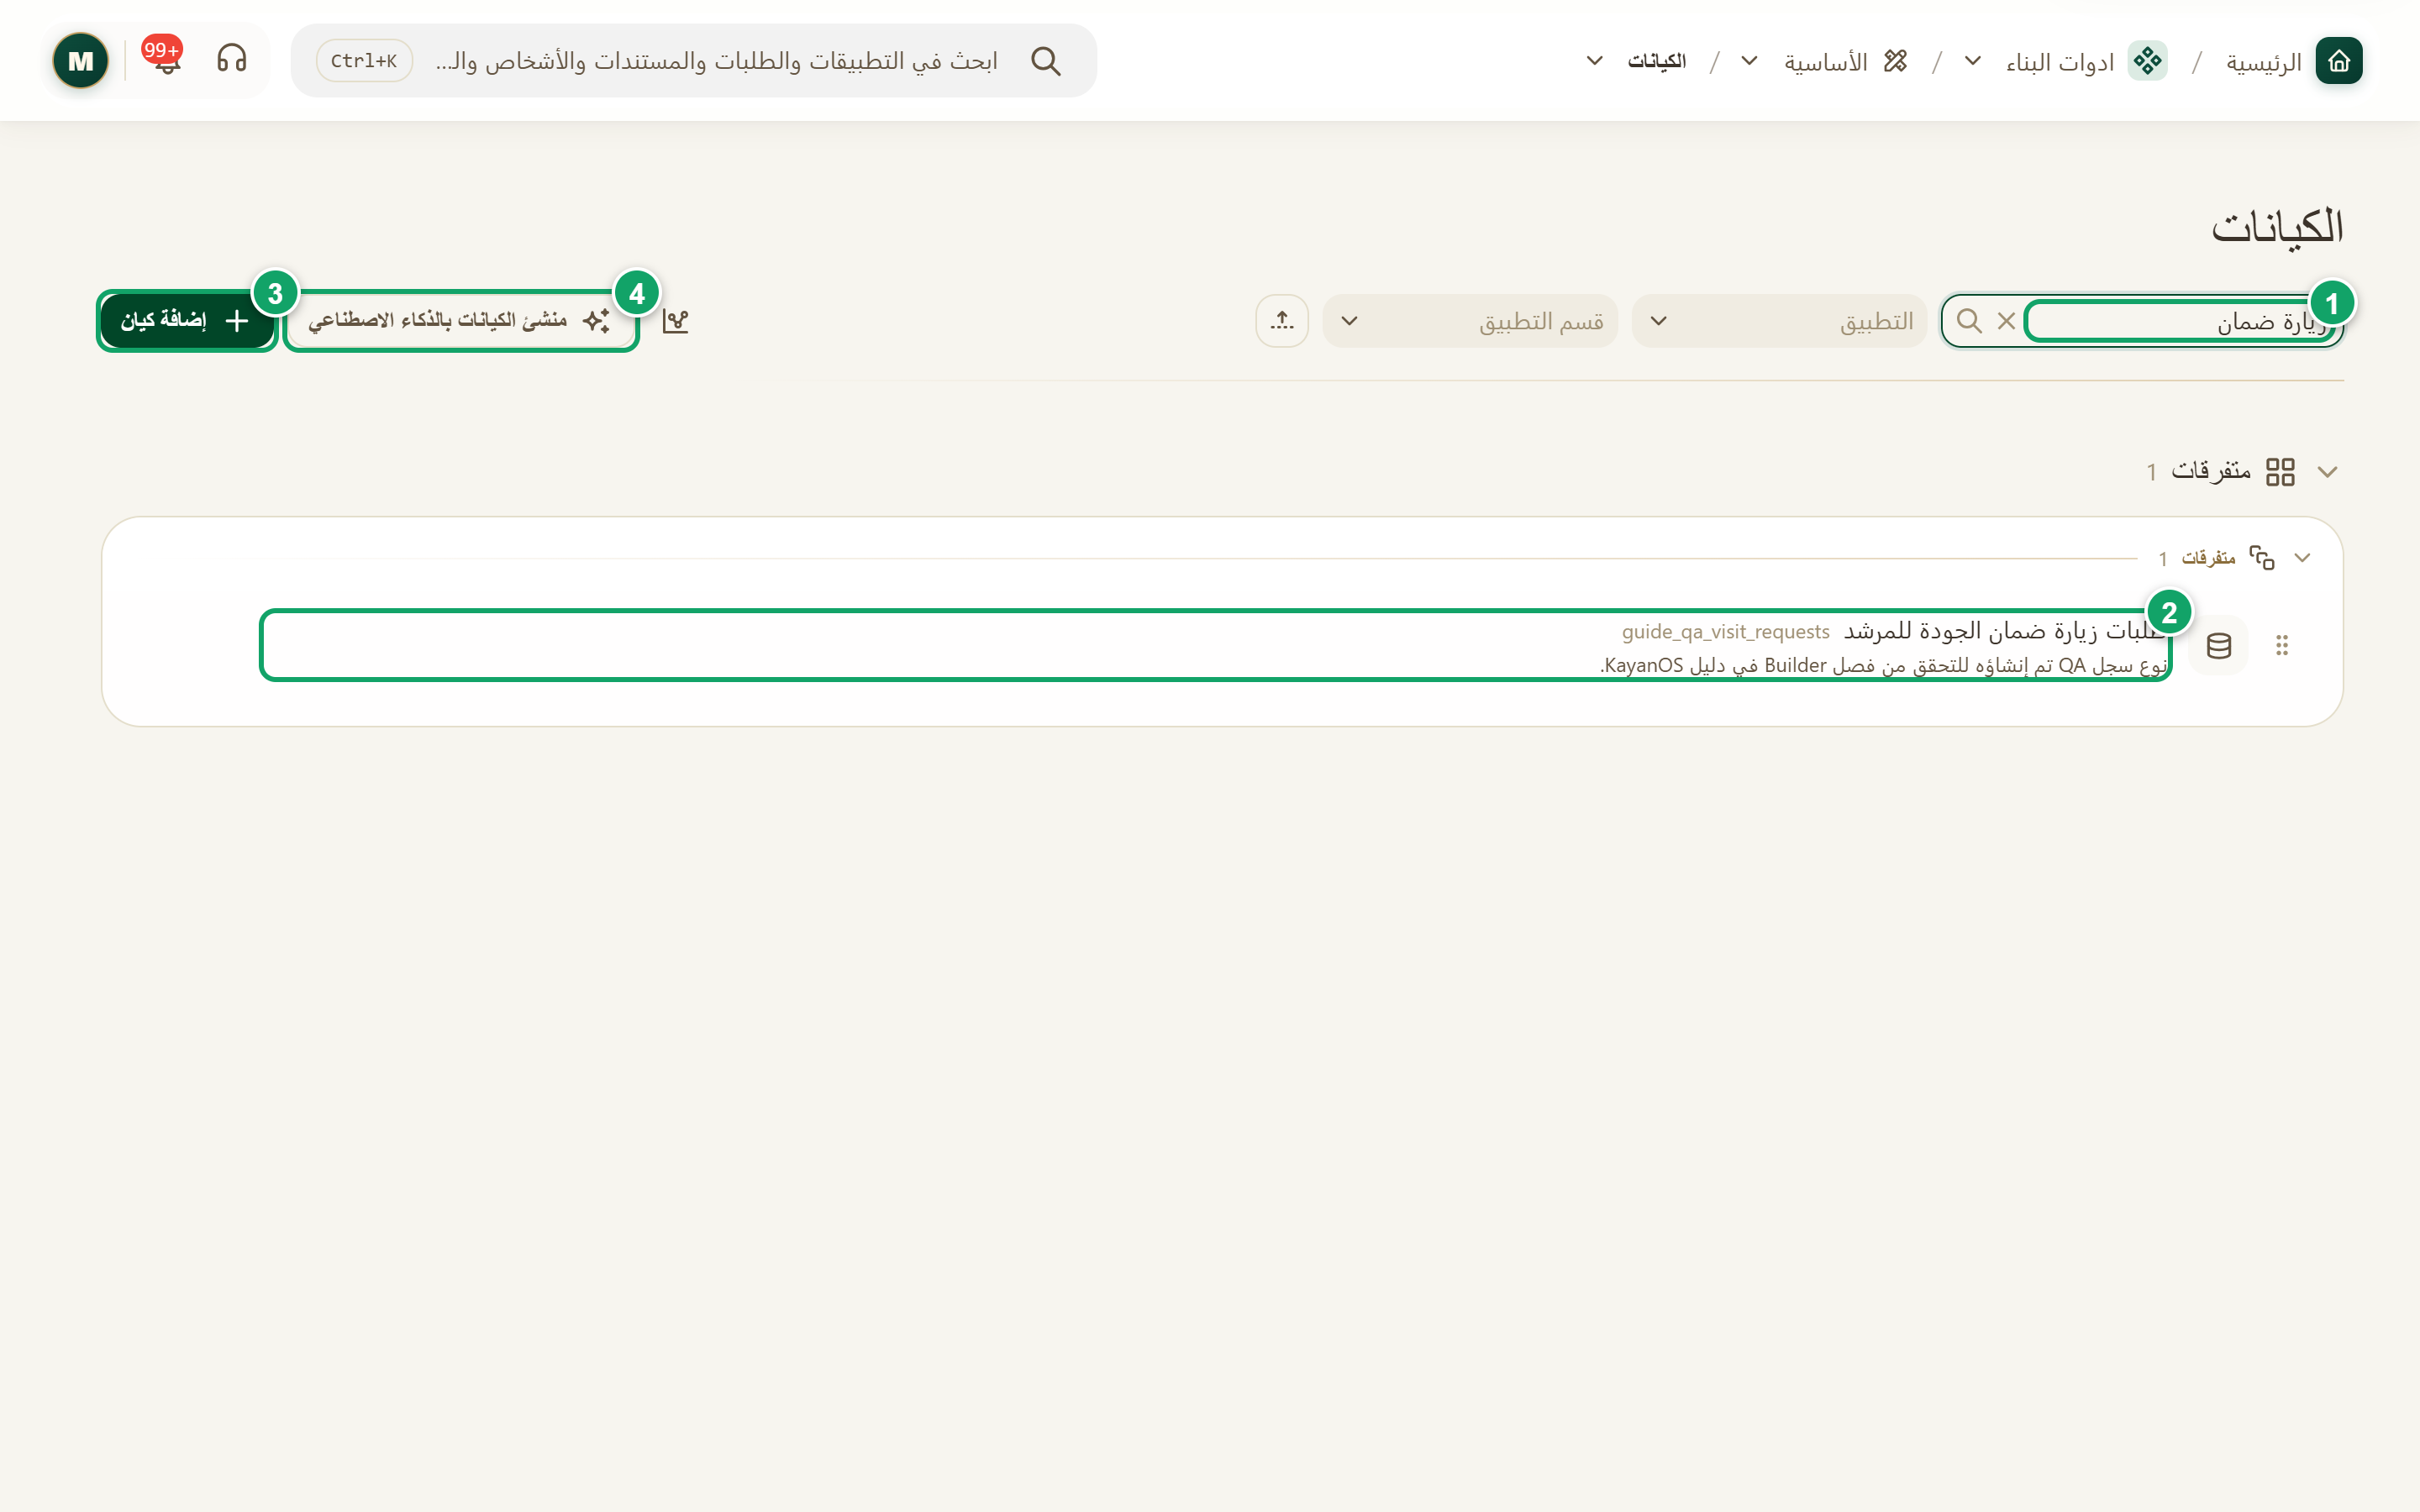
\includegraphics[width=0.95\linewidth,height=0.72\textheight,keepaspectratio]{figures/screens/ch06-entities-ar.png}
\caption{صفحة «الكيانات» بعد البحث عن نوع سجلات}
\label{fig:builder-entities-screen}
\shotnote{تعرض الصفحة أنواع السجلات مجمّعة حسب التطبيق، وهنا ضُيّقت القائمة بالبحث فظهر نوع سجلات اختباري واحد أُنشئ في test2 للتحقق من هذا الفصل. ① مربع البحث: اكتب جزءاً من اسم النوع قبل أن تنشئ نوعاً جديداً. ② النوع الذي وجدته: اضغطه لتفتحه في «المنشئ». ③ «إضافة كيان»: تنشئ نوعاً جديداً عندما لا تجد ما تحتاجه. ④ «منشئ الكيانات بالذكاء الاصطناعي»: يقترح الحقول من وصف تكتبه.}
\end{figure}


\begin{table}[H]
\centering
\caption{ما الذي تجده هنا؟}
\label{tab:builder-entities-data}
\begin{tabularx}{\linewidth}{R{3.6cm} Y}
\rcHeaderRow
\thh{القسم} & \thh{المحتوى والإجراء}\\
قائمة الأنواع & أنواع السجلات مجمّعة حسب التطبيق والقسم، ولكل نوع اسمه ومفتاحه ووصفه. تضيّق القائمة بالبحث أو بفلترَي «التطبيق» و«قسم التطبيق».\\
إضافة كيان & يفتح صفحة تكتب فيها عنوان النوع ووصفه وحقوله الأولى، ثم تضغط «انشاء كيان».\\
منشئ الكيانات بالذكاء الاصطناعي & تصف النوع الذي تريده بكلماتك، فيقترح النظام حقوله لتراجعها قبل الحفظ. يظهر الزر فقط إذا فعّلت المؤسسة الذكاء الاصطناعي في أدوات البناء.\\
عرض مخطط العلاقات & يرسم أنواع السجلات والعلاقات بينها، فتعرف ما يرتبط بالنوع قبل تعديله.\\
فتح نوع موجود & الضغط على النوع يفتحه في «المنشئ»، حيث تعدّل حقوله وصفحته وقوائمه وتنشر التغييرات.\\
\end{tabularx}
\end{table}

\begin{figure}[H]
\centering
\begin{tikzpicture}[node distance=0.5cm]
\node[stepBox] (a) {\RL{البحث عن نوع مشابه}};
\node[stepBox,below=of a] (b) {\RL{إضافة كيان وكتابة عنوانه}};
\node[stepBox,below=of b] (c) {\RL{انشاء كيان}};
\node[stepBox,below=of c] (d) {\RL{فتحه في المنشئ}};
\draw[flowsTo] (a) -- (b);
\draw[flowsTo] (b) -- (c);
\draw[flowsTo] (c) -- (d);
\end{tikzpicture}
\rclegend
\caption{خطوات إنشاء نوع سجلات}
\label{fig:builder-entities-flow}
\shotnote{يبدأ المخطط بالبحث لأن النوع الذي تحتاجه قد يكون موجوداً في تطبيق جاهز، وإنشاء نسخة ثانية منه يفرّق البيانات بين مكانين. وبعد «انشاء كيان» تعود إلى قائمة الكيانات، ثم تفتح النوع الجديد في «المنشئ» لتكمل بناءه، فالإنشاء لا يعني أن التطبيق صار جاهزاً للفريق.}
\end{figure}

\subsection{خطوات العمل والتحقق}
\begin{enumerate}
\item افتح «الكيانات» واكتب في البحث اسماً قريباً مما تحتاجه، ثم راجع النتائج قبل أن تنشئ نوعاً جديداً.
\item اضغط «إضافة كيان»، واكتب عنواناً بصيغة الجمع يصف السجلات، مثل «طلبات الصيانة»، ثم أضف وصفاً قصيراً.
\item سمِّ الحقل الأول المقترح أو غيّر نوعه، واضغط «اضافة حقل جديد» لكل معلومة أساسية أخرى.
\item اضغط زر الإعدادات بجانب «انشاء كيان» لتختار التطبيق والقسم اللذين يظهر فيهما النوع، ثم اضغط «انشاء كيان».
\end{enumerate}

\textbf{تحقق ومعالجة المشكلة:} يجب أن تظهر رسالة نجاح وأن يظهر النوع الجديد في قائمة «الكيانات» تحت التطبيق الذي اخترته. فإذا بقي زر «انشاء كيان» معطلاً، فاكتب عنوان النوع أولاً؛ وإذا لم تجد النوع في القائمة، فأزل فلترَي التطبيق والقسم وابحث باسمه.

\clearpage
\section{منشئ الكيانات بالذكاء الاصطناعي ومخطط العلاقات}
\label{sec:builder-feature-ai-builder}

بدلاً من إضافة الحقول واحداً بعد الآخر، يمكنك أن تصف نوع السجلات الذي تحتاجه بكلماتك، فيقترح «منشئ الكيانات بالذكاء الاصطناعي» حقوله وتبويباته وأقسامه، ثم تراجع الاقتراح وتعدّله قبل حفظه. وتفيدك هذه الطريقة عندما يكون النوع كبيراً أو عندما تريد نقطة بداية سريعة. أما «عرض مخطط العلاقات» فيرسم أنواع السجلات الموجودة والعلاقات بينها، فتعرف قبل أي تعديل ما الذي يرتبط بالنوع الذي ستغيّره.

\textbf{المسار ومن يستخدمه:} «الكيانات» ← «منشئ الكيانات بالذكاء الاصطناعي»، أو زر «عرض مخطط العلاقات» في رأس الصفحة نفسها. يظهر زر الذكاء الاصطناعي عندما يكون «الذكاء الاصطناعي في أدوات البناء» مفعّلاً في إعدادات المؤسسة، ويحتاج الحفظ إلى صلاحيات إنشاء الكيانات وتعديلها وإنشاء الحقول.

\begin{rcnote}[مثال: شركة الأفق]
يكتب مسؤول النظام في الأفق: «أنشئ نوع سجلات لطلبات زيارة الفروع، فيه الفرع وتاريخ الزيارة وغرضها ومقدّم الطلب». ثم يجيب عن سؤالين يطرحهما المساعد، ويراجع الحقول المقترحة، ويضغط «تحقق» قبل «حفظ الكيان».
\end{rcnote}

\begin{figure}[H]
\centering
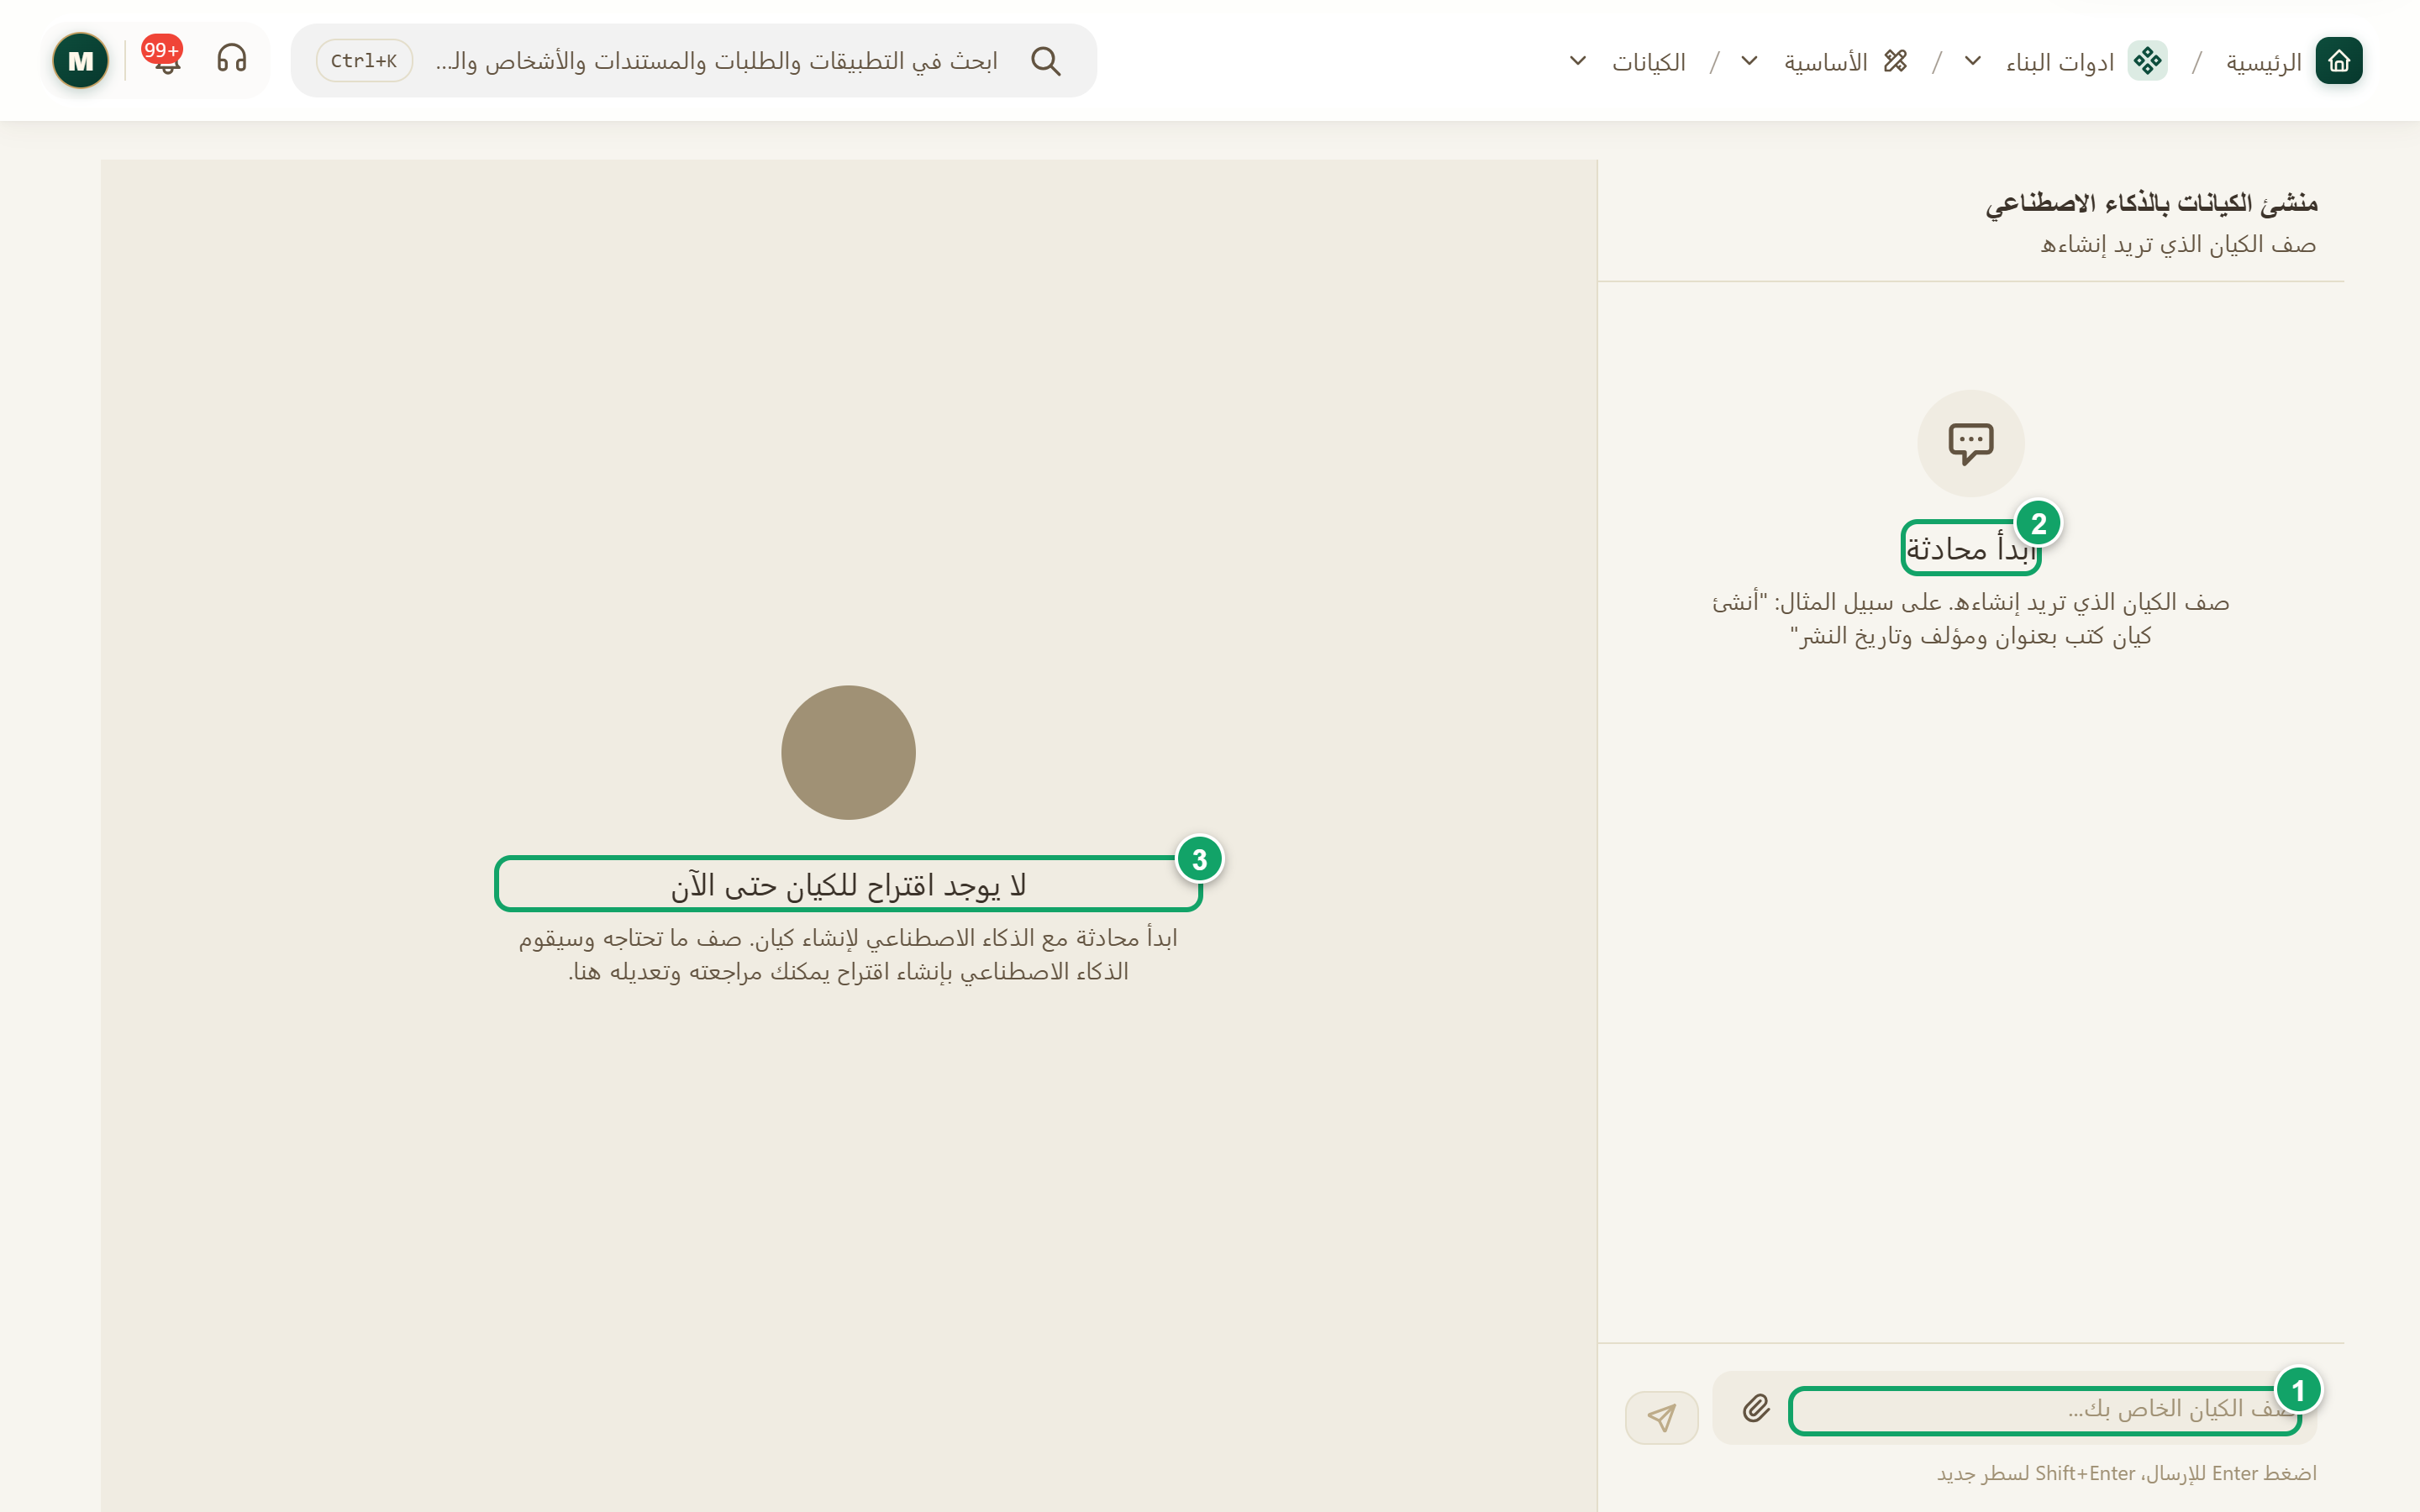
\includegraphics[width=0.95\linewidth,height=0.72\textheight,keepaspectratio]{figures/screens/ch06-ai-builder-ar.png}
\caption{منشئ الكيانات بالذكاء الاصطناعي قبل بدء المحادثة}
\label{fig:builder-ai-builder-screen}
\shotnote{تعرض الشاشة المساعد قبل أي محادثة: المحادثة في جهة، ومعاينة الاقتراح في الجهة الأخرى وهي فارغة حتى يقترح المساعد نوعاً. وتفيدك الصورة في معرفة مكان الكتابة ومكان مراجعة النتيجة قبل الحفظ. ① مربع «صف الكيان الخاص بك...»: تكتب فيه وصف النوع. ② «ابدأ محادثة»: مثال على وصف مناسب تسترشد به. ③ «لا يوجد اقتراح للكيان حتى الآن»: مكان «معاينة الكيان» الذي يمتلئ بعد أول اقتراح.}
\end{figure}

\begin{table}[H]
\centering
\caption{ما الذي تجده في المنشئ بالذكاء الاصطناعي؟}
\label{tab:builder-ai-builder-parts}
\begin{tabularx}{\linewidth}{R{3.6cm} Y}
\rcHeaderRow
\thh{الجزء} & \thh{ما يقدمه}\\
المحادثة & تصف النوع في مربع «صف الكيان الخاص بك...»، ويمكنك أن ترفق ملفاً يشرح عملك. وقد يطرح المساعد أسئلة توضيحية، فتجيب عنها ثم تضغط «إرسال الإجابات».\\
معاينة الكيان & تعرض الاقتراح كاملاً: المفتاح والعنوان والوصف، والتبويبات والأقسام، والإجراءات المخصصة، وجدول الحقول. ويمكنك أن تعدّل أي جزء منه قبل الحفظ.\\
تحقق & يفحص الاقتراح، ويعرض ما يجده في «مشاكل التحقق» مع اقتراح لإصلاح كل مشكلة. والأخطاء تمنع الحفظ، أما التحذيرات فلا تمنعه.\\
اطلب من الذكاء الاصطناعي الإصلاح & يرسل المشكلات إلى المحادثة، فيصحّح المساعد اقتراحه بدلاً من أن تعدّله يدوياً.\\
حفظ الكيان & ينشئ النوع وحقوله بعد «تأكيد الحفظ». ولا يعمل الزر إلا بعد تحقق ناجح دون أخطاء، وبعد آخر تعديل أجريته.\\
تحميل JSON & يحفظ الاقتراح ملفاً تحتفظ به أو تشاركه مع زميل للمراجعة.\\
مخطط العلاقات & يعرض كل نوع مع حقوله، ويرسم العلاقات أسهماً تحمل اسم الحقل الذي يربط بينها. والضغط على نوع يبرز علاقاته، و«تحميل البنية» يحفظ وصفاً نصياً لكل الأنواع وعلاقاتها.\\
\end{tabularx}
\end{table}

\begin{rcwarn}[الحفظ هنا لا يمر بمسودة]
على خلاف «المنشئ»، يُنشأ النوع وحقوله مباشرة بعد «تأكيد الحفظ»، ثم تعود إلى قائمة «الكيانات». لذلك راجع الاقتراح جيداً قبل الحفظ، ثم افتح النوع في «المنشئ» لتكمل صفحته وقواعده وصلاحياته. وإذا كان الاقتراح يعدّل نوعاً موجوداً، فالحفظ يضيف الحقول الجديدة فقط ولا يغيّر الحقول القائمة.
\end{rcwarn}

\begin{figure}[H]
\centering
\begin{tikzpicture}[node distance=0.5cm]
\node[stepBox] (a) {\RL{وصف النوع في المحادثة}};
\node[stepBox,below=of a] (b) {\RL{الإجابة عن الأسئلة}};
\node[stepBox,below=of b] (c) {\RL{مراجعة معاينة الكيان}};
\node[stepBox,below=of c] (d) {\RL{تحقق}};
\node[stepBox,below=of d] (e) {\RL{حفظ الكيان}};
\node[stepBox,below=of e] (f) {\RL{إكماله في المنشئ}};
\draw[flowsTo] (a) -- (b);
\draw[flowsTo] (b) -- (c);
\draw[flowsTo] (c) -- (d);
\draw[flowsTo] (d) -- (e);
\draw[flowsTo] (e) -- (f);
\end{tikzpicture}
\rclegend
\caption{إنشاء نوع سجلات بمساعدة الذكاء الاصطناعي}
\label{fig:builder-ai-builder-flow}
\shotnote{يضع المخطط «تحقق» قبل الحفظ لأن الزر لا يعمل دونه، ولأن كل تعديل في المعاينة يتطلب تحققاً جديداً. أما الخطوة الأخيرة فتذكّرك بأن المساعد يقترح الحقول والتبويبات فقط، وأن صفحة السجل وقواعده وصلاحياته تُضبط بعد ذلك في «المنشئ».}
\end{figure}

\subsection{خطوات العمل والتحقق}
\begin{enumerate}
\item افتح «الكيانات» واضغط «عرض مخطط العلاقات»، وابحث عن نوع قريب مما تحتاجه حتى لا تكرر نوعاً موجوداً.
\item اضغط «منشئ الكيانات بالذكاء الاصطناعي»، واكتب وصفاً يذكر ما يمثله السجل والمعلومات التي يحفظها، ثم اضغط \en{Enter}.
\item أجب عن الأسئلة التوضيحية إن ظهرت، واضغط «إرسال الإجابات».
\item راجع «معاينة الكيان»: اسم النوع ومفتاحه، وأنواع الحقول، والتبويبات. وعدّل ما يلزم مباشرة أو اطلب التعديل في المحادثة.
\item اضغط «تحقق»، وأصلح الأخطاء بنفسك أو بزر «اطلب من الذكاء الاصطناعي الإصلاح»، ثم اضغط «حفظ الكيان» و«تأكيد الحفظ».
\end{enumerate}

\textbf{تحقق ومعالجة المشكلة:} يجب أن تظهر رسالة «تم حفظ الكيان بنجاح» وأن يظهر النوع في قائمة «الكيانات». فإذا بقي «حفظ الكيان» معطلاً، فاضغط «تحقق» مرة أخرى بعد آخر تعديل، أو مرّر المؤشر فوقه لترى الصلاحيات الناقصة. وإذا لم يظهر زر الذكاء الاصطناعي أصلاً، فاطلب من مسؤول المؤسسة تفعيل «الذكاء الاصطناعي في أدوات البناء».

\clearpage
\section{المنشئ والنظرة العامة}
\label{sec:builder-feature-workspace}

«المنشئ» هو مساحة العمل التي تعدّل فيها نوع السجلات بعد إنشائه، وتفتحه بالضغط على النوع في صفحة «الكيانات». وتظهر أقسامه في قائمة جانبية بالترتيب: «نظرة عامة»، و«الحقول»، و«صفحة السجل»، و«القوائم وطرق العرض»، و«القواعد»، و«الصلاحيات»، و«الحركة»، و«الإثبات»، و«الإجراءات والأتمتة»، و«الاستيراد»، و«إعدادات متقدمة». ويلخّص قسم «نظرة عامة» حالة النوع كلها في مكان واحد، وينبّهك إلى ما يجب إصلاحه قبل النشر.

\textbf{المسار ومن يستخدمه:} «الكيانات» ← اضغط نوع السجلات ← «نظرة عامة». يستخدمه من يبني النوع في كل مرة يعود إليه، ليعرف ما تغيّر وما بقي ناقصاً.

\begin{rcnote}[مثال: شركة الأفق]
يفتح المسؤول «طلبات الزيارة» فيرى في «نظرة عامة» أن ثلاثة حقول لم توضع بعد في أي صفحة، وأن قائمة «قبل النشر» تعرض تحذيراً لتسمية بلا نص إنجليزي. فيضع الحقول في الصفحة ويترجم التسمية، ثم يضغط «المراجعة والنشر».
\end{rcnote}

\begin{figure}[H]
\centering
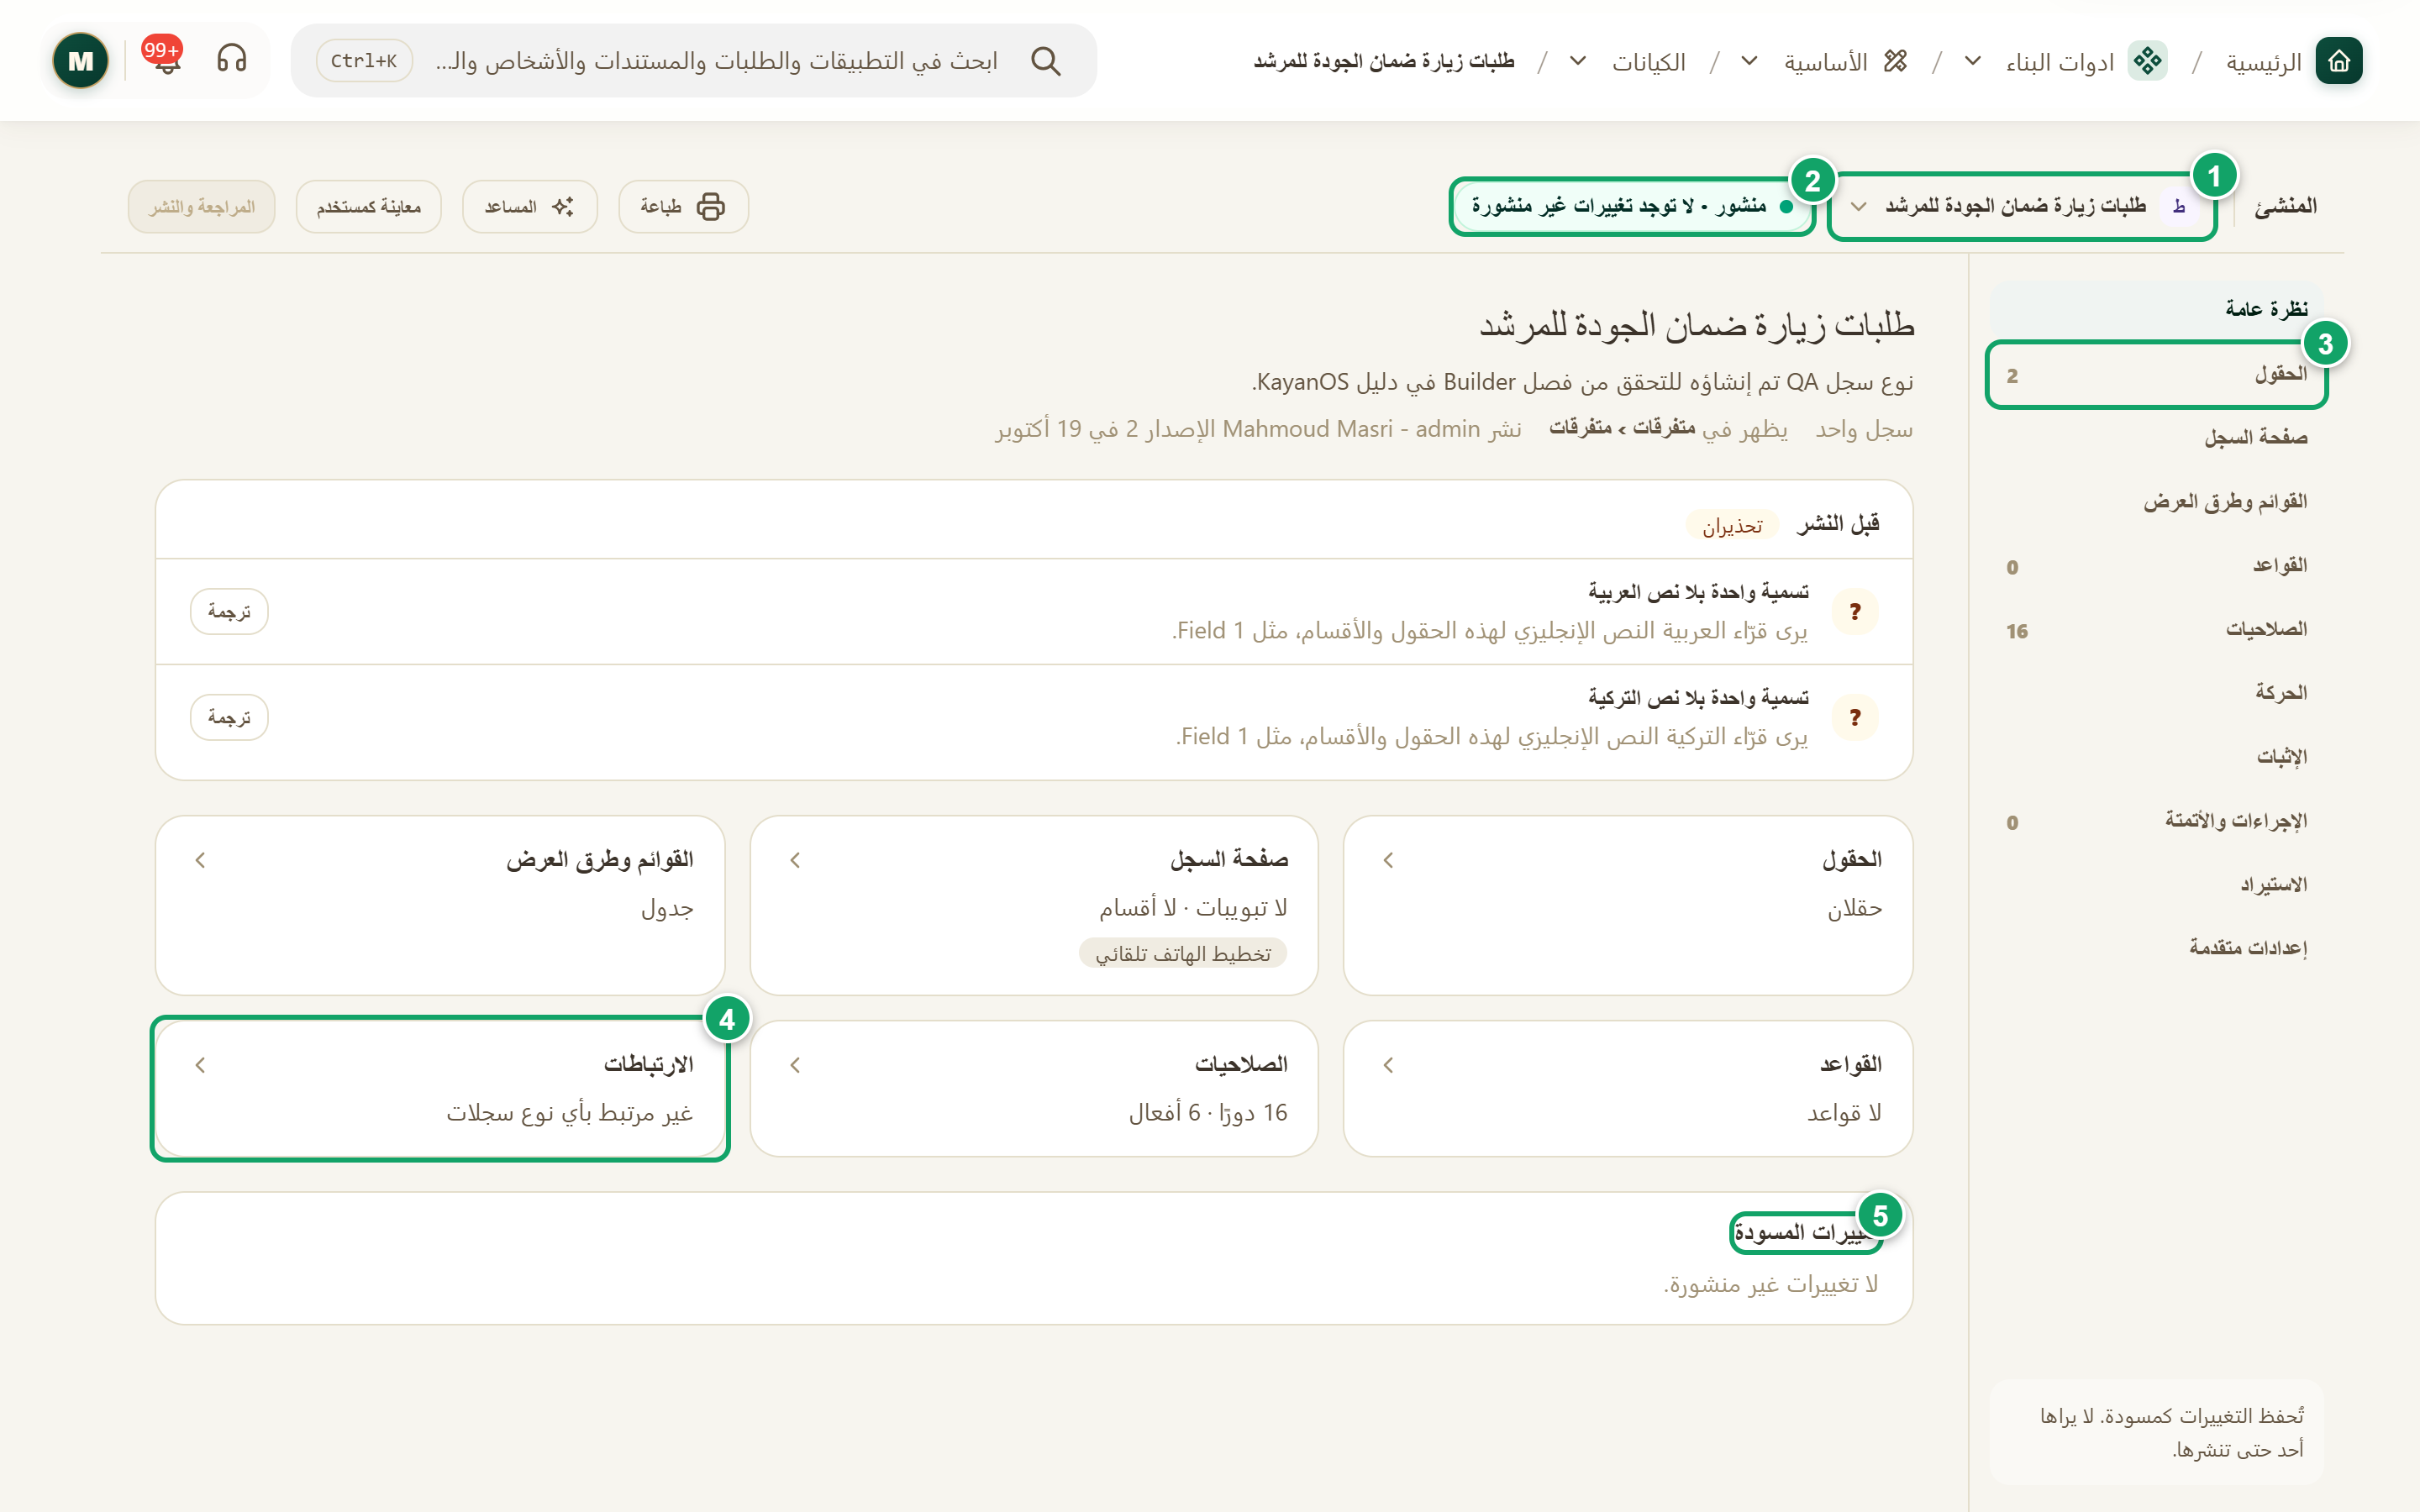
\includegraphics[width=0.95\linewidth,height=0.72\textheight,keepaspectratio]{figures/screens/ch06-ws-header-ar.png}
\caption{رأس المنشئ وقسم «نظرة عامة» لنوع سجلات اختباري}
\label{fig:builder-workspace-screen}
\shotnote{تعرض الصورة نوع السجلات الاختباري الذي أُنشئ في test2 للتحقق من هذا الدليل، مفتوحاً في «المنشئ» على «نظرة عامة». ويجمع الرأس والقائمة الجانبية والبطاقات كل ما تحتاج إلى معرفته قبل أي تعديل. ① تبديل نوع السجلات. ② شارة الحالة: تقول إن النوع منشور ولا تغييرات معلّقة. ③ «الحقول» في القائمة الجانبية: الرقم بجانبها عدد الحقول. ④ بطاقة «الارتباطات». ⑤ «تغييرات المسودة»: ما لم يُنشر بعد.}
\end{figure}

\begin{table}[H]
\centering
\caption{رأس المنشئ}
\label{tab:builder-workspace-header}
\begin{tabularx}{\linewidth}{R{3.6cm} Y}
\rcHeaderRow
\thh{العنصر} & \thh{ما يقدمه}\\
تبديل نوع السجلات & ينقلك إلى نوع آخر دون العودة إلى القائمة، وفيه بحث «ابحث عن نوع سجلات».\\
شارة الحالة & تقول «منشور · لا توجد تغييرات غير منشورة» عندما يطابق النوع ما يراه الفريق، أو «مسودة» مع عدد التغييرات غير المنشورة ووقت آخر حفظ.\\
طباعة & يفتح قوالب الطباعة الخاصة بنوع السجلات، ويظهر عددها بجانب الزر عند وجودها.\\
المساعد & يفتح «مساعد البناء»، فتطلب منه حقلاً أو قاعدة أو معادلة، فيقترح تغييرات على المسودة وتطبّق منها ما تريد. ولا يُنشر شيء حتى تراجع وتنشر.\\
معاينة كمستخدم & تعرض صفحة السجل كما يراها دور أو شخص بعينه، دون أن يُحفظ شيء.\\
المراجعة والنشر · N & يفتح نافذة المراجعة، والرقم عدد التغييرات في المسودة. ولا يعمل الزر إذا لم تكن هناك تغييرات.\\
\end{tabularx}
\end{table}

\begin{table}[H]
\centering
\caption{أجزاء «نظرة عامة»}
\label{tab:builder-workspace-cards}
\begin{tabularx}{\linewidth}{R{3.6cm} Y}
\rcHeaderRow
\thh{الجزء} & \thh{ما يخبرك به}\\
رأس الصفحة & اسم النوع ووصفه، وعدد السجلات، والتطبيق والقسم في «يظهر في»، والإصدار المنشور ومن نشره. ومنه تفتح قائمة السجلات بزر «فتح القائمة».\\
الحقول & عدد الحقول، والمحسوبة والمجمّعة منها، والحقول التي لم توضع في أي صفحة.\\
صفحة السجل & عدد التبويبات والأقسام، وهل كتل النظرة العامة مفعّلة.\\
القوائم وطرق العرض & طرق العرض المتاحة والافتراضية منها، وعدد المؤشرات والعروض المحفوظة.\\
القواعد & عدد القواعد موزعاً حسب نوعها، مثل الإظهار والإخفاء والتعديل والإلزام.\\
الصلاحيات & عدد الأدوار والأفعال والأفعال المخصصة، والحقول التي لها صلاحيات خاصة.\\
الارتباطات & عدد أنواع السجلات المرتبطة بهذا النوع، فتعرف ما قد يتأثر بتعديله.\\
تغييرات المسودة & التغييرات غير المنشورة منذ بدء المسودة، ومنها تفتح المراجعة بزر «مراجعة الكل».\\
قبل النشر & المشكلات التي تمنع النشر والتحذيرات، ولكل مشكلة زر يفتح مكان إصلاحها.\\
\end{tabularx}
\end{table}

\subsection{قائمة «قبل النشر»}

تفحص هذه القائمة المسودة كلما عدّلتها. فبعض المشكلات يمنع النشر لأن السجلات لن تعمل معها، مثل قاعدة أو صيغة تشير إلى حقل محذوف، أو تعبير فيه خطأ، أو خيارات قائمة فارغة أو مكررة، أو حذف الحقل الذي يحمل اسم السجل. أما التحذيرات فلا تمنع النشر لكنها تستحق المراجعة، مثل تبويب يبقى فارغاً دائماً، أو حقل وُضع في تبويب غير موجود، أو تسميات بلا ترجمة. وعندما تخلو القائمة يظهر «لا شيء يحتاج إلى إصلاح. يمكن نشر المسودة.».

\begin{rcwarn}[عندما يعدّل شخصان المسودة نفسها]
إذا حفظ شخص آخر المسودة بعد أن فتحتها، تظهر رسالة «غيّر شخص آخر هذه المسودة»، ولا تُحفظ تعديلاتك حتى تختار. اضغط «تحميل مسودته» لترى نسخته وتفقد تعديلاتك غير المحفوظة، أو «استبدالها بنسختي» لتحفظ نسختك فوقها. وقد ظهرت هذه الرسالة أثناء اختبار هذا الدليل لنسخة قديمة من الجلسة نفسها، فإن كنت متأكداً أن أحداً لا يعدّل النوع معك فاختر «استبدالها بنسختي».
\end{rcwarn}

\begin{figure}[H]
\centering
\begin{tikzpicture}[node distance=0.5cm]
\node[stepBox] (a) {\RL{فتح النوع من الكيانات}};
\node[stepBox,below=of a] (b) {\RL{قراءة نظرة عامة}};
\node[stepBox,below=of b] (c) {\RL{التعديل في الأقسام}};
\node[stepBox,below=of c] (d) {\RL{إصلاح ما في قبل النشر}};
\node[stepBox,below=of d] (e) {\RL{المراجعة والنشر}};
\draw[flowsTo] (a) -- (b);
\draw[flowsTo] (b) -- (c);
\draw[flowsTo] (c) -- (d);
\draw[flowsTo] (d) -- (e);
\end{tikzpicture}
\rclegend
\caption{جلسة عمل في المنشئ}
\label{fig:builder-workspace-flow}
\shotnote{يبدأ المخطط بقراءة «نظرة عامة» لأنها تبيّن لك حالة النوع قبل أن تغيّر شيئاً، وينتهي بالنشر لأن التعديلات تبقى في المسودة حتى ذلك الحين. وتقع خطوة «قبل النشر» قبل المراجعة مباشرة، لأن مشكلة واحدة تمنع النشر كله حتى تُصلحها.}
\end{figure}

\subsection{خطوات العمل والتحقق}
\begin{enumerate}
\item افتح «الكيانات» واضغط نوع السجلات، فيفتح «المنشئ» على «نظرة عامة».
\item اقرأ شارة الحالة: إذا كانت «مسودة» فهناك تغييرات سابقة لم تُنشر، فراجعها من «تغييرات المسودة» قبل أن تضيف غيرها.
\item انتقل إلى القسم الذي تريد تعديله من القائمة الجانبية، وعدّل ما تحتاج إليه؛ فكل تعديل يُحفظ في المسودة تلقائياً.
\item عُد إلى «نظرة عامة»، واضغط زر الإصلاح بجانب كل مشكلة في «قبل النشر» حتى تخلو القائمة من الأخطاء.
\end{enumerate}

\textbf{تحقق ومعالجة المشكلة:} يجب أن تتغير شارة الحالة إلى «مسودة» مع عدد التغييرات بعد كل تعديل، وأن يصبح زر «المراجعة والنشر» متاحاً. فإذا ظهر «تعذّر الحفظ، سنعيد المحاولة عند التغيير التالي»، فتحقق من اتصالك ثم عدّل أي قيمة ليُعاد الحفظ.

\clearpage
\section{الحقول}
\label{sec:builder-feature-fields}

يحدد الحقل معلومة واحدة يحفظها كل سجل، مثل التاريخ أو المبلغ أو الشخص المسؤول. واختيار نوع الحقل المناسب مهم، لأنه يحدد طريقة الإدخال والتحقق من القيمة، ويسمح بالترتيب والتصفية والحساب لاحقاً. وتضيف الحقول من قسم «الحقول» في «المنشئ».

\textbf{المسار ومن يستخدمه:} «الكيانات» ← افتح نوع السجلات ← «الحقول». يستخدمه من يبني نوع السجلات، قبل ترتيب الصفحة والقوائم.

\begin{rcnote}[مثال: شركة الأفق]
يضيف مسؤول النظام إلى «طلبات الزيارة» حقل «معرف تسلسلي» يعطي كل طلب رقماً مثل \en{HZN-VR-0001}، ثم حقل «علاقة» يربط الطلب بالفرع، وحقل «تاريخ» لموعد الزيارة، وحقل «نص طويل» لغرضها. وتطابق خطواته في الصورة الرقمين ① و③.
\end{rcnote}

\begin{figure}[H]
\centering
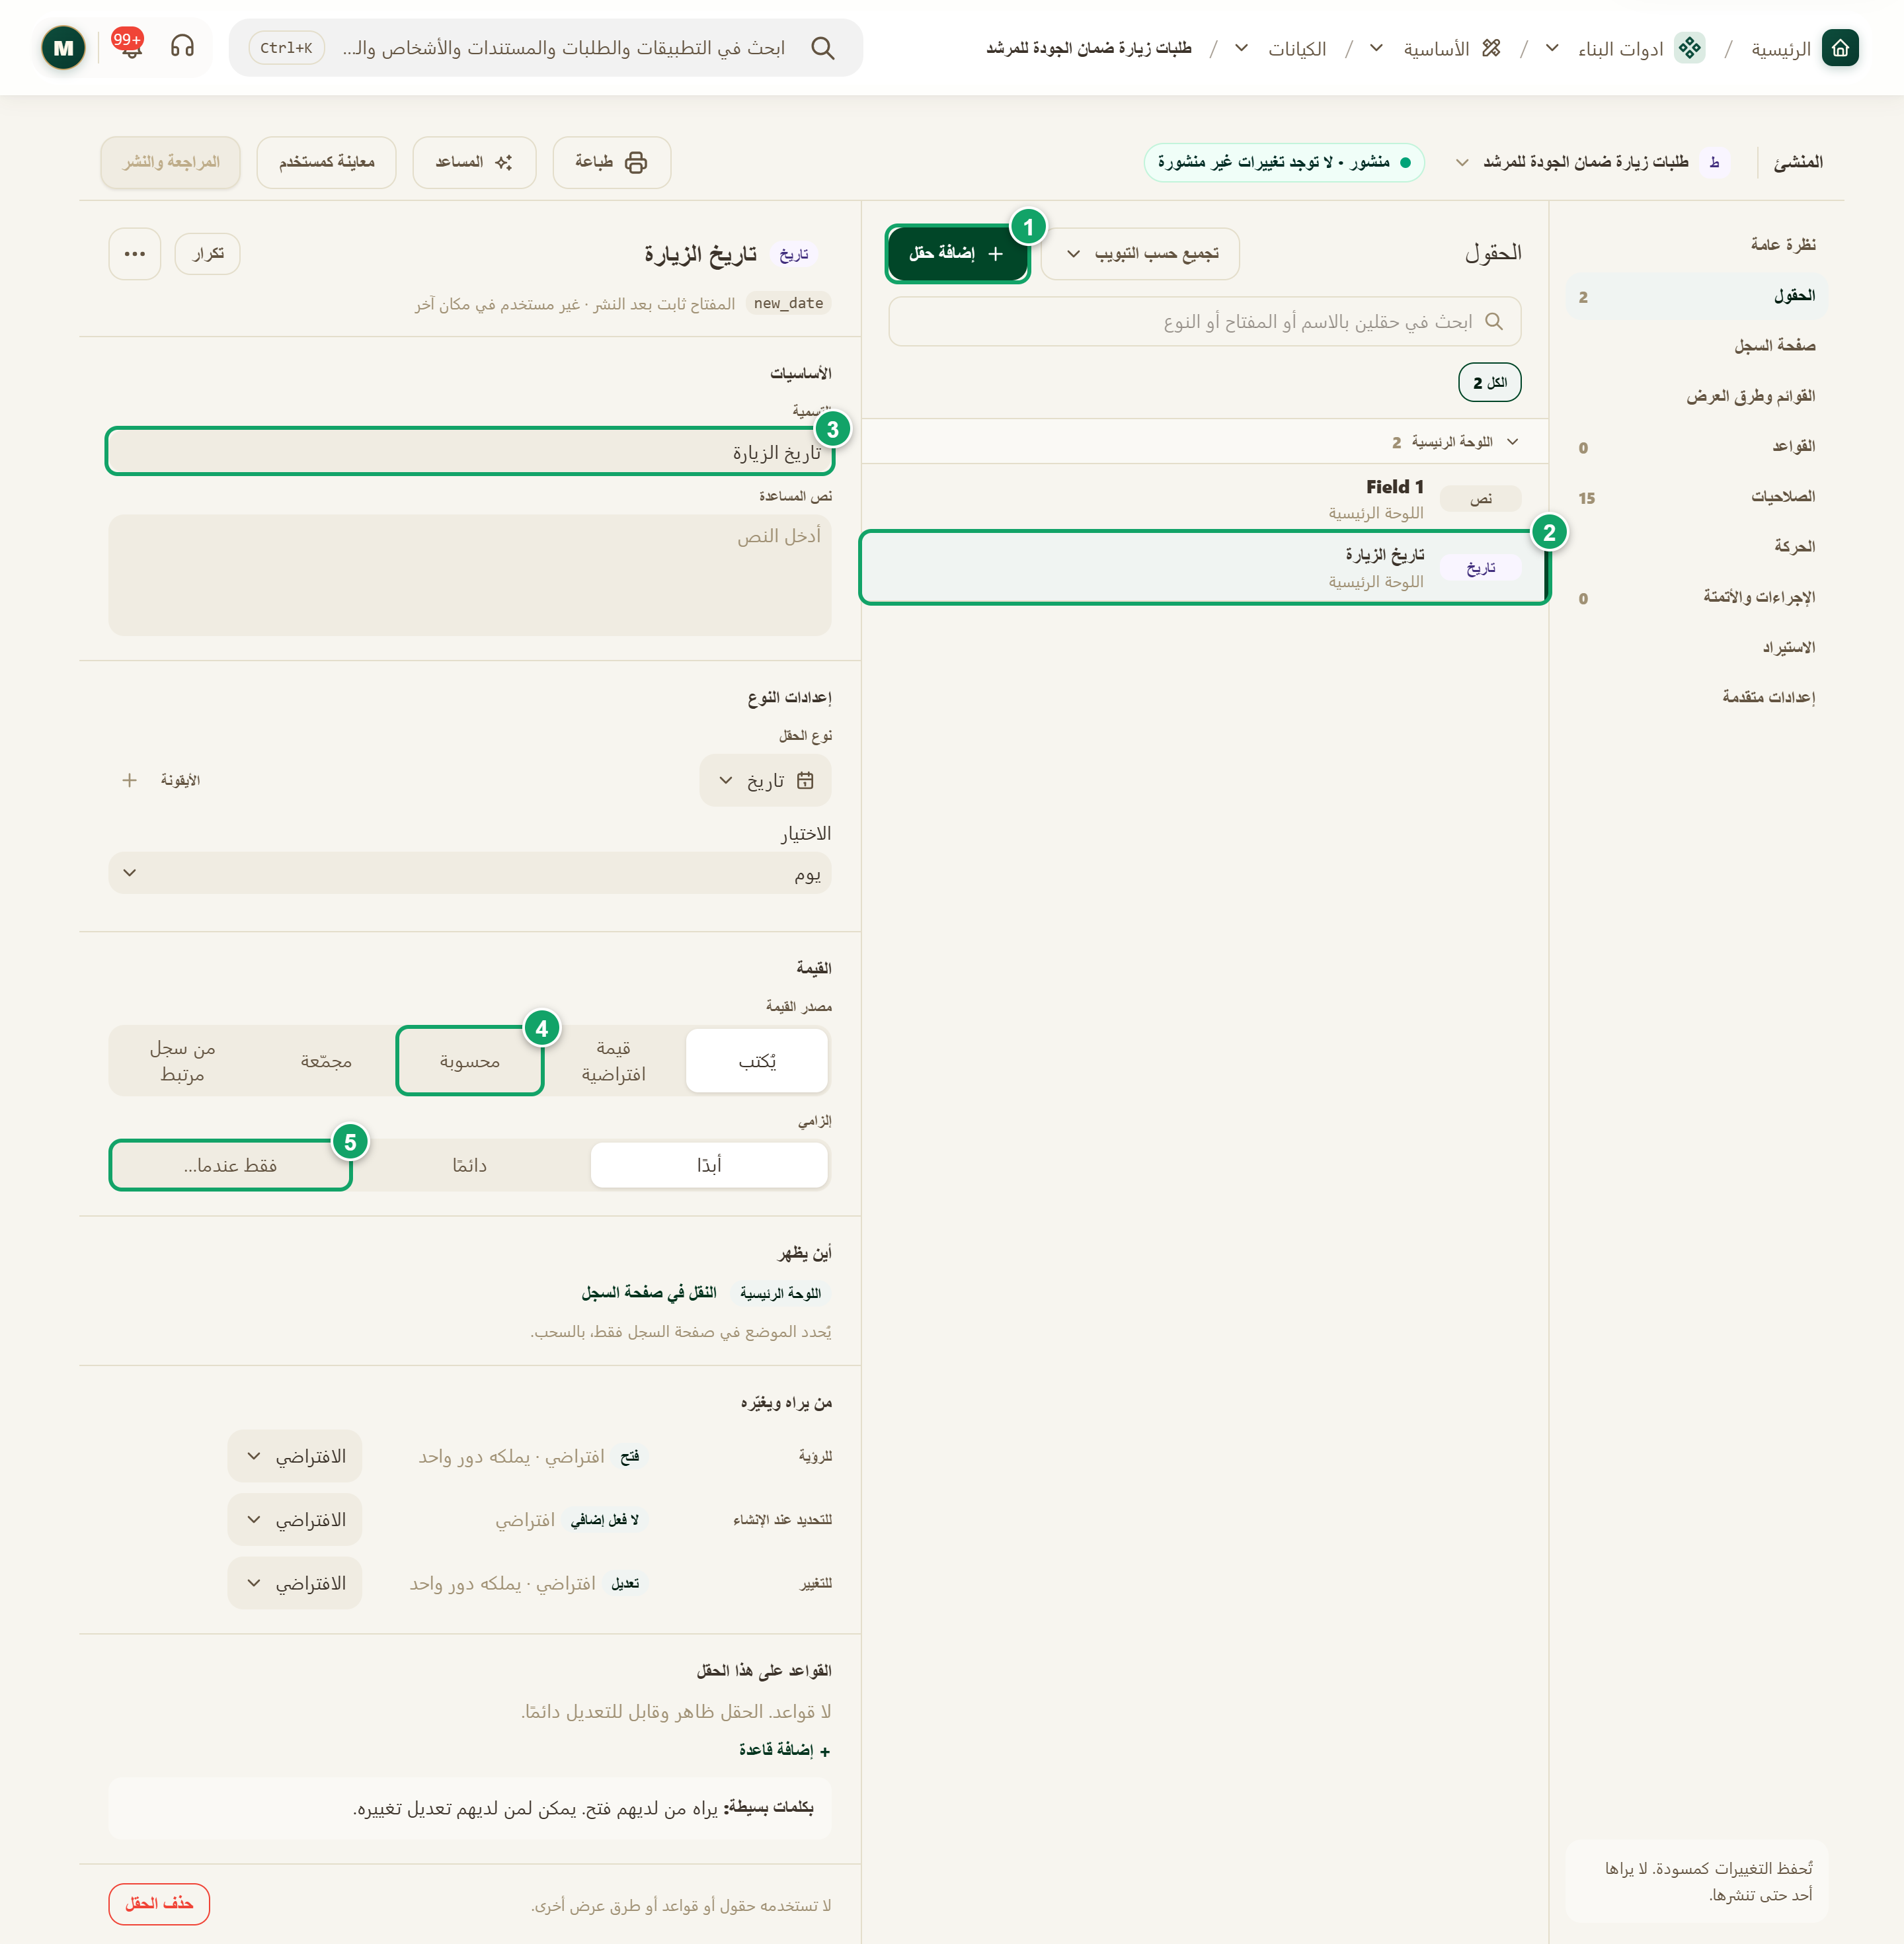
\includegraphics[width=0.95\linewidth,height=0.72\textheight,keepaspectratio]{figures/screens/ch06-ws-fields-ar.png}
\caption{قسم «الحقول» وإعدادات حقل تاريخ}
\label{fig:builder-fields-screen}
\shotnote{يعرض القسم قائمة حقول نوع السجلات، وعند اختيار حقل تظهر إعداداته بجانبه. والحقل المختار هنا حقل «تاريخ» أُضيف ونُشر أثناء اختبار هذا الفصل على test2. ① «إضافة حقل». ② الحقل المختار في القائمة. ③ «التسمية». ④ «محسوبة»: تجعل القيمة ناتج صيغة بدلاً من أن يكتبها المستخدم. ⑤ «فقط عندما…»: تجعل الحقل إلزامياً في حالة معينة.}
\end{figure}


\begin{table}[H]
\centering
\caption{أنواع الحقول}
\label{tab:builder-fields-types}
\begin{tabularx}{\linewidth}{R{3.6cm} Y}
\rcHeaderRow
\thh{المجموعة} & \thh{الأنواع ومتى تستخدمها}\\
النصوص & «نص» لقيمة قصيرة، و«نص طويل» للوصف، و«نص منسّق» لنص بتنسيق، و«هاتف» لرقم الهاتف.\\
الأرقام والمعرّفات & «رقم» للكميات والمبالغ، و«المدة» للزمن المستغرق، و«معرف تسلسلي» لرقم مرجعي يولّده النظام لكل سجل.\\
التواريخ والأوقات & «تاريخ» و«تاريخ ووقت» و«وقت»، والنطاقات منها مثل «نطاق التاريخ» عندما يكون للمعلومة بداية ونهاية.\\
الاختيار والحالة & «اختيار» لقائمة قيم محددة، و«قيمة منطقية» لإجابة نعم أو لا، و«الحالة» لمراحل العمل وفق قالب حالات.\\
الملفات والصور & «ملف» للمرفقات، و«صورة رمزية» لصورة تمثّل السجل.\\
الروابط والأشخاص & «علاقة» لربط السجل بسجل من نوع آخر، و«اختيار عضو» لتحديد عضو من المؤسسة.\\
الخرائط & «موقع» لنقطة على الخريطة، و«حدود» لمساحة مرسومة مثل حدود عقار أو منشأة.\\
إجراء & حقل متقدم يعمل مع قسم «الإجراءات والأتمتة».\\
محسوبة ومرتبطة ومجمّعة & قيم لا يكتبها المستخدم: «محسوبة» بصيغة من حقول السجل، و«مرتبطة» تعرض قيمة من سجل مرتبط، و«مجمّعة» تجمع قيم السجلات المرتبطة أو تعدّها.\\
\end{tabularx}
\end{table}

\begin{table}[H]
\centering
\caption{ما الذي تضبطه في كل حقل؟}
\label{tab:builder-fields-settings}
\begin{tabularx}{\linewidth}{R{3.6cm} Y}
\rcHeaderRow
\thh{الإعداد} & \thh{المعنى}\\
التسمية & الاسم الذي يراه المستخدم، ويمكن كتابته بأكثر من لغة.\\
المفتاح & اسم ثابت يستخدمه النظام في الصيغ والقوالب. اختره واضحاً من البداية، لأن الإشارات إليه تعتمد عليه.\\
نص المساعدة & جملة قصيرة تشرح للمستخدم ما يكتبه في الحقل.\\
إلزامي & يمنع حفظ السجل إذا بقي الحقل فارغاً. استخدمه للمعلومات التي لا يكتمل العمل دونها فقط.\\
\end{tabularx}
\end{table}

\begin{figure}[H]
\centering
\begin{tikzpicture}[node distance=0.5cm]
\node[stepBox] (a) {\RL{إضافة حقل}};
\node[stepBox,below=of a] (b) {\RL{اختيار نوع الحقل}};
\node[stepBox,below=of b] (c) {\RL{التسمية والمفتاح}};
\node[stepBox,below=of c] (d) {\RL{الإلزام ونص المساعدة}};
\draw[flowsTo] (a) -- (b);
\draw[flowsTo] (b) -- (c);
\draw[flowsTo] (c) -- (d);
\end{tikzpicture}
\rclegend
\caption{خطوات إضافة حقل}
\label{fig:builder-fields-flow}
\shotnote{يضع المخطط اختيار النوع قبل التسمية، لأن النوع يحدد الإعدادات التي تظهر بعده، مثل خيارات القائمة في «اختيار» أو النوع المرتبط في «علاقة». وتُحفظ كل إضافة في المسودة فوراً، لكن المستخدمين لا يرون الحقل الجديد حتى تنشر التغييرات.}
\end{figure}

\subsection{خطوات العمل والتحقق}
\begin{enumerate}
\item افتح نوع السجلات من «الكيانات»، ثم اختر قسم «الحقول».
\item اضغط «إضافة حقل»، واختر النوع الذي يطابق المعلومة؛ فالتاريخ مثلاً يُحفظ في حقل «تاريخ» لا في «نص».
\item اكتب التسمية وراجع المفتاح، وأضف نص مساعدة عند الحاجة، ثم حدد إن كان الحقل إلزامياً.
\item لحقل يُحسب من غيره، اختر «محسوبة» واكتب الصيغة؛ ولقيمة من سجل مرتبط، اختر «حقل مرتبط» بعد إضافة حقل «علاقة».
\end{enumerate}

\textbf{تحقق ومعالجة المشكلة:} يجب أن يظهر الحقل في قائمة الحقول، وأن تعرض «نظرة عامة» عدده مع الحقول التي لم توضع بعد في أي صفحة. فإذا اخترت نوعاً خاطئاً، فصحّحه قبل النشر وقبل إدخال سجلات حقيقية، لأن تغيير النوع بعد تراكم البيانات أصعب.

\clearpage
\section{أنواع الحقول وإعداداتها}
\label{sec:builder-feature-field-types}

يحدد نوع الحقل شكل الإدخال، والتحقق من القيمة، وما يمكن فعله بها لاحقاً من ترتيب وتصفية وحساب. ولذلك تشرح هذه الصفحة كل الأنواع المتاحة في «إضافة حقل»، ثم الإعدادات الإضافية التي تظهر في «إعدادات النوع» لبعضها. واختر النوع قبل إدخال بيانات حقيقية، لأن تغييره بعد تراكم السجلات أصعب.

\textbf{المسار ومن يستخدمه:} «المنشئ» ← «الحقول» ← «إضافة حقل»، ثم «إعدادات النوع» في لوحة إعدادات الحقل. يستخدمه من يبني نوع السجلات.

\begin{rcnote}[مثال: شركة الأفق]
يختار مسؤول النظام لحقل رقم الطلب نوع «معرف تسلسلي» بوضع «تلقائي»، ويكتب له تنسيقاً يبدأ بـ \en{HZN-VR-} فيحمل أول طلب الرقم \en{HZN-VR-0001}. ويختار لحقل الفرع نوع «علاقة» يرتبط بنوع سجلات الفروع.
\end{rcnote}

\begin{figure}[H]
\centering
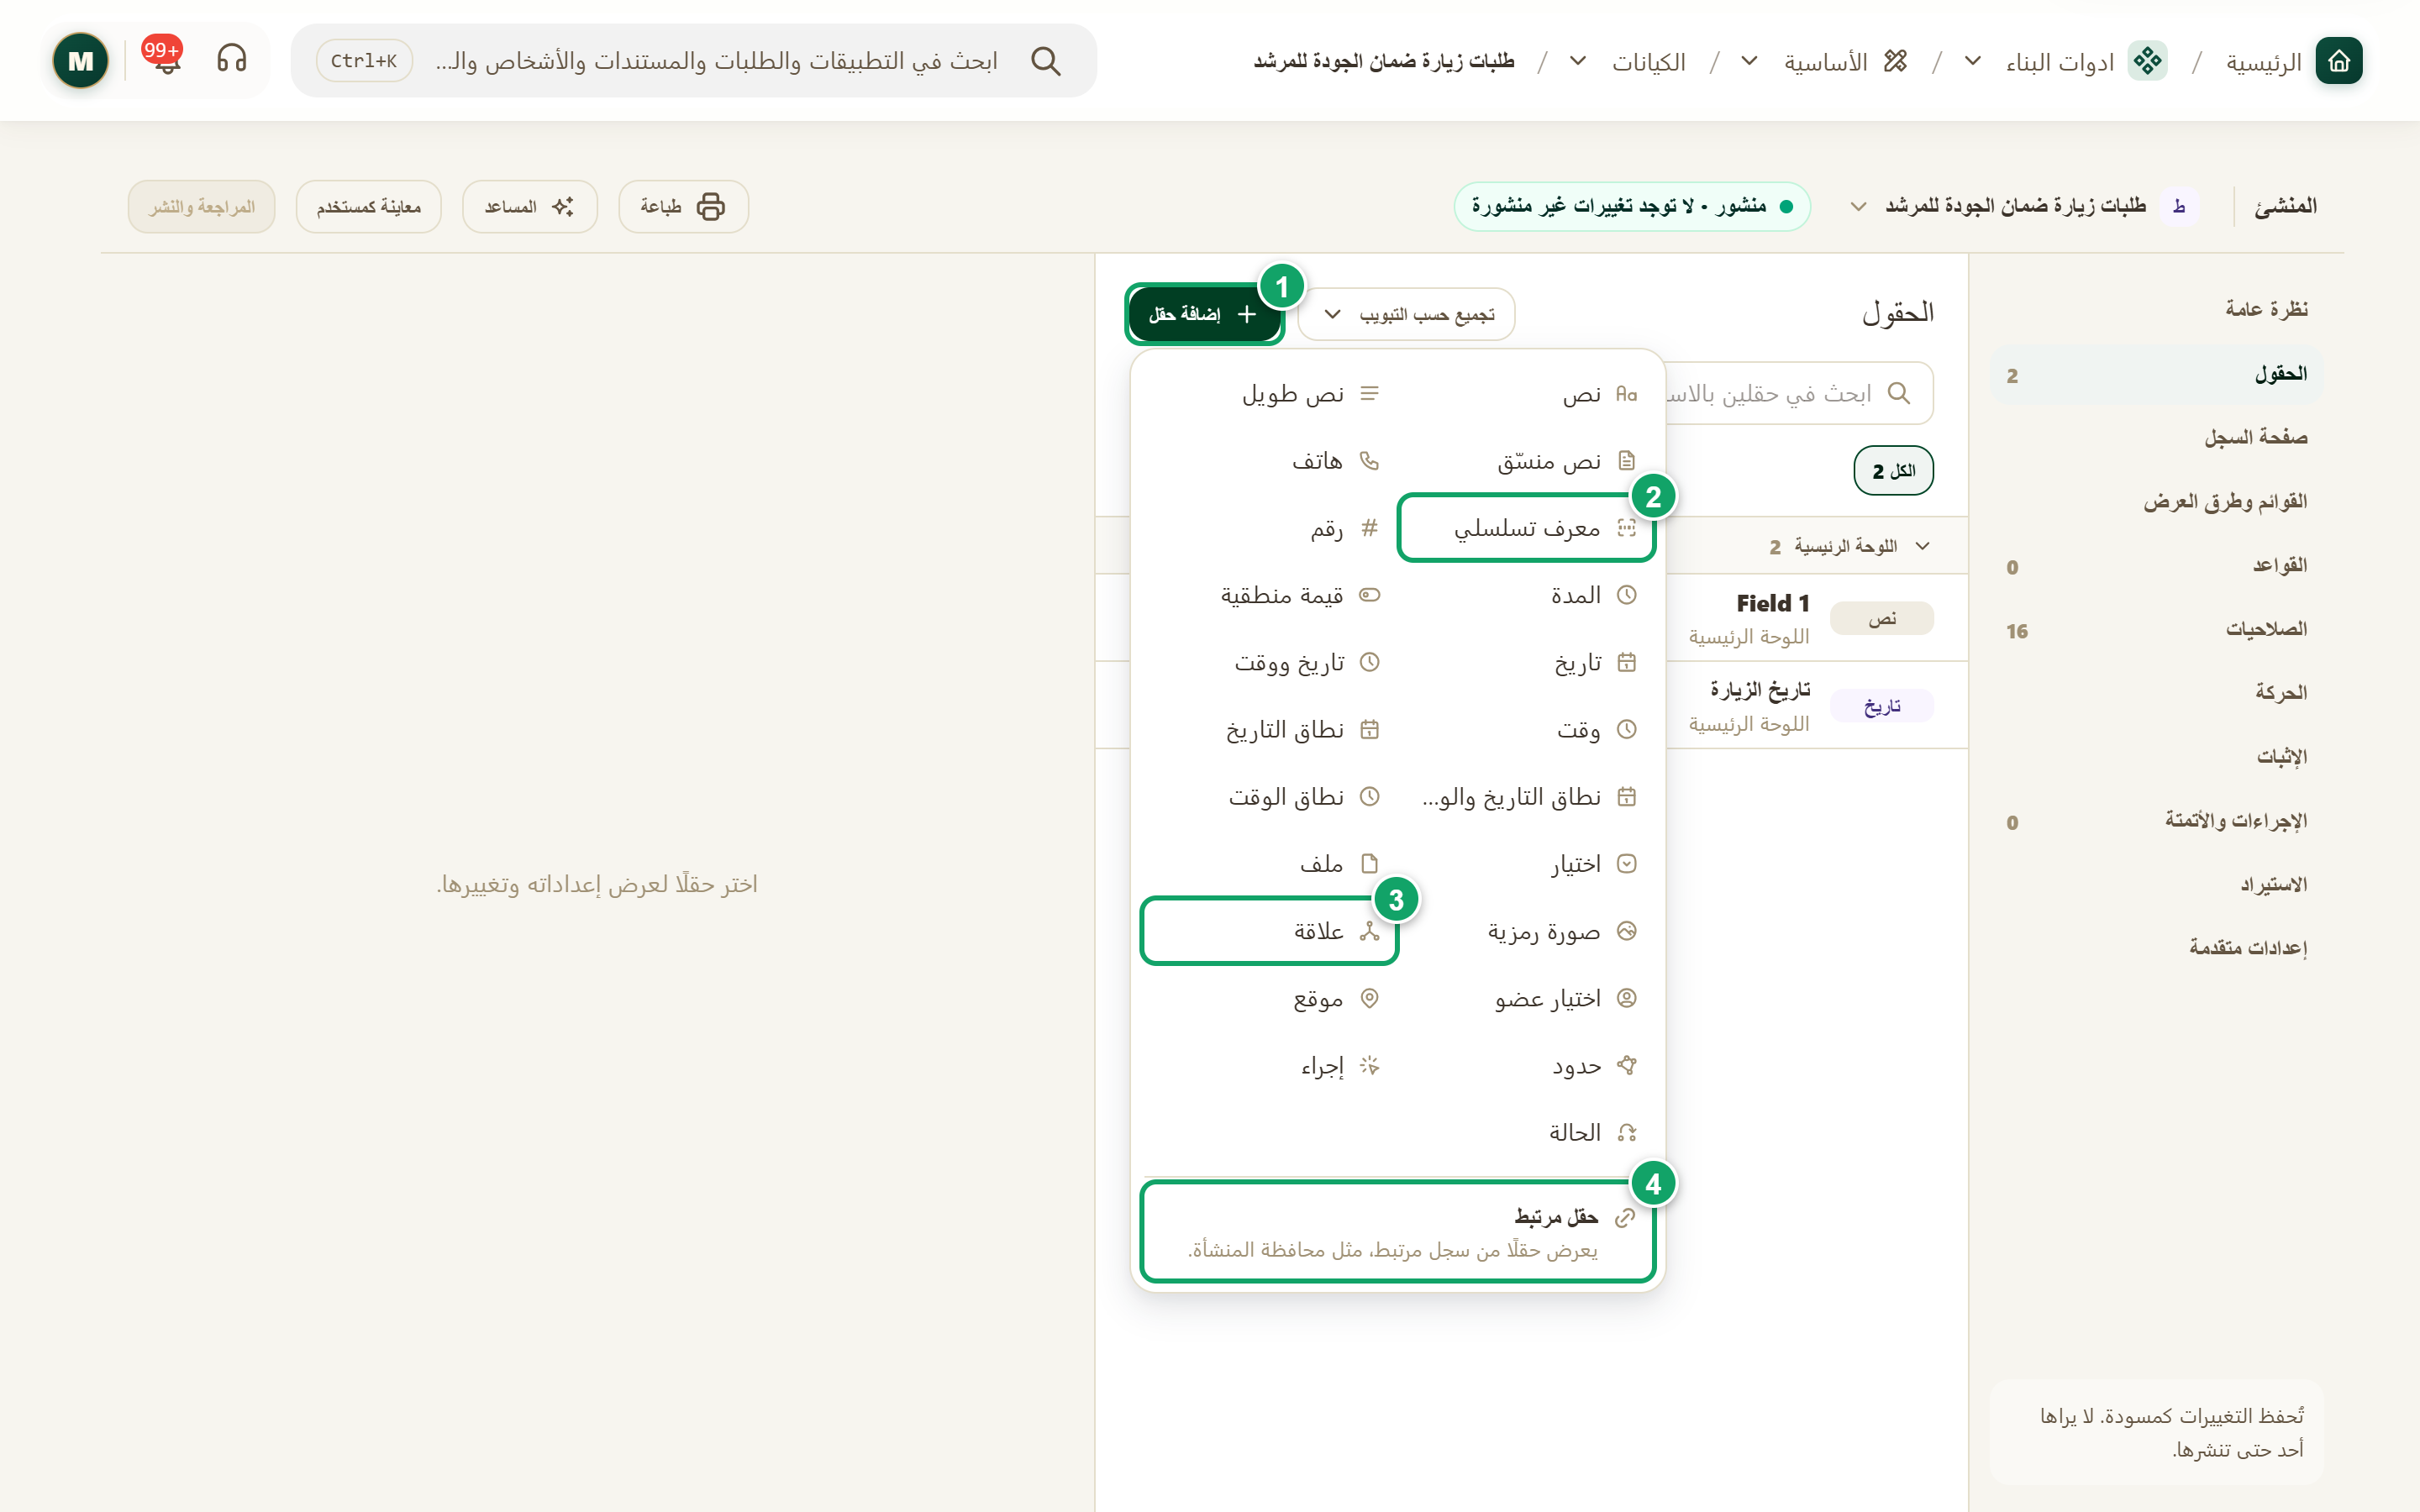
\includegraphics[width=0.95\linewidth,height=0.72\textheight,keepaspectratio]{figures/screens/ch06-ws-add-field-ar.png}
\caption{قائمة أنواع الحقول بعد الضغط على «إضافة حقل»}
\label{fig:builder-field-types-screen}
\shotnote{تعرض الصورة القائمة التي تفتح عند إضافة حقل، وفيها كل الأنواع المتاحة بالترتيب الذي تظهر به. ويفيدك ذلك في اختيار النوع الصحيح من البداية بدلاً من تغييره بعد إدخال البيانات. ① «إضافة حقل». ② «معرف تسلسلي»: لرقم مرجعي يولّده النظام. ③ «علاقة»: لربط السجل بسجل من نوع آخر. ④ «حقل مرتبط»: لعرض معلومة من سجل مرتبط.}
\end{figure}

\begin{table}[H]
\centering
\caption{الأنواع المتاحة في «إضافة حقل»}
\label{tab:builder-field-types-all}
\begin{tabularx}{\linewidth}{R{3.6cm} Y}
\rcHeaderRow
\thh{المجموعة} & \thh{الأنواع ومتى تستخدم كلاً منها}\\
النصوص & «نص» لقيمة قصيرة كالاسم، و«نص طويل» لوصف أو ملاحظة، و«نص منسّق» لنص فيه عناوين وقوائم، و«هاتف» لرقم الهاتف.\\
الأرقام والمعرّفات & «رقم» للكميات والمبالغ، و«المدة» لزمن مستغرق مثل ساعتين، و«معرف تسلسلي» لرقم مرجعي يولّده النظام لكل سجل.\\
نعم أو لا & «قيمة منطقية» لسؤال جوابه نعم أو لا، مثل «تحتاج إلى سيارة؟».\\
التواريخ والأوقات & «تاريخ» و«تاريخ ووقت» و«وقت» لقيمة واحدة، و«نطاق التاريخ» و«نطاق التاريخ والوقت» و«نطاق الوقت» لمعلومة لها بداية ونهاية.\\
الاختيار والحالة & «اختيار» لقائمة قيم ثابتة، و«الحالة» لمراحل العمل وفق قالب حالات، مثل «جديد» ثم «قيد المراجعة» ثم «معتمد».\\
الروابط والأشخاص & «علاقة» لربط السجل بسجل من نوع آخر، و«اختيار عضو» لتحديد عضو من المؤسسة، و«حقل مرتبط» لعرض معلومة من سجل مرتبط دون إعادة كتابتها.\\
الملفات والصور & «ملف» للمرفقات، و«صورة رمزية» لصورة تمثّل السجل في القوائم والبطاقات.\\
الخرائط & «موقع» لنقطة على الخريطة، و«حدود» لمساحة مرسومة على الخريطة مع مساحتها ومحيطها، مثل حدود عقار أو منشأة.\\
إجراء & زر داخل السجل يُنشئ مستند Word أو جدول Excel، أو يفتح رابطاً، أو يبدأ مسار عمل.\\
\end{tabularx}
\end{table}

\begin{table}[H]
\centering
\caption{إعدادات إضافية حسب النوع}
\label{tab:builder-field-types-settings}
\begin{tabularx}{\linewidth}{R{3.6cm} Y}
\rcHeaderRow
\thh{النوع} & \thh{ما تضبطه في «إعدادات النوع»}\\
اختيار والحالة & «الخيارات» وألوانها، و«السماح بإضافة خيارات» إذا أردت أن يضيف المستخدم قيمة جديدة، وقيمة رقمية لكل خيار عند الحاجة إلى حسابات.\\
علاقة & «مرتبط بـ» لتختار نوع السجلات الآخر، وما يحدث للسجل عند حذف السجل المرتبط: منع الحذف، أو تفريغ الحقل، أو حذف السجلات التابعة معه. وتختار في «عرض العلاقة في التبويب» و«طريقة عرض العلاقات» كيف تظهر هذه السجلات في صفحة السجل الآخر، ومن ذلك «قائمة تحقق» يُجاب عن بنودها في مكانها.\\
معرف تسلسلي & «وضع سلسلة»: «تلقائي» أو «عند الطلب» أو كلاهما، و«إدخال الرقم التسلسلي يدويًا»، و«تنسيق JEXL» الذي يحدد شكل الرقم، و«ابدأ من» و«المنطقة الزمنية».\\
الحالة & قالب الحالات الذي يحدد المراحل: «قالب ثابت» لكل السجلات، أو «قالب لكل سجل» يُختار من حقل آخر.\\
اختيار عضو & «طريقة العرض»: بيانات العضو حقولاً داخل القسم، أو تبويباً مستقلاً في صفحة السجل.\\
ملف & حدود للملفات أضيق من حدود المؤسسة، مثل أنواع الملفات المسموح بها.\\
موقع وحدود & صيغة الإحداثيات: خط العرض وخط الطول، أو \en{MGRS}، أو \en{UTM}.\\
كل الأنواع & «السماح بعدة قيم» لحفظ أكثر من قيمة في الحقل نفسه، و«نص لكل لغة» لنص يُكتب بالعربية والإنجليزية.\\
\end{tabularx}
\end{table}

\begin{figure}[H]
\centering
\begin{tikzpicture}[node distance=0.5cm]
\node[stepBox] (a) {\RL{إضافة حقل}};
\node[stepBox,below=of a] (b) {\RL{اختيار النوع المطابق}};
\node[stepBox,below=of b] (c) {\RL{إعدادات النوع}};
\node[stepBox,below=of c] (d) {\RL{قيمة واحدة أم عدة قيم}};
\node[stepBox,below=of d] (e) {\RL{تجربته في سجل}};
\draw[flowsTo] (a) -- (b);
\draw[flowsTo] (b) -- (c);
\draw[flowsTo] (c) -- (d);
\draw[flowsTo] (d) -- (e);
\end{tikzpicture}
\rclegend
\caption{اختيار نوع الحقل وضبطه}
\label{fig:builder-field-types-flow}
\shotnote{يجعل المخطط «إعدادات النوع» خطوة مستقلة لأن بعض الأنواع لا تعمل دونها: فحقل «علاقة» يحتاج إلى النوع المرتبط، و«اختيار» يحتاج إلى خياراته. أما الخطوة الأخيرة فتذكّرك بتجربة الحقل في سجل حقيقي بعد النشر، لأن شكل الإدخال لا يظهر كاملاً إلا هناك.}
\end{figure}

\subsection{خطوات العمل والتحقق}
\begin{enumerate}
\item في «الحقول» اضغط «إضافة حقل»، واختر النوع الذي يطابق المعلومة لا شكلها؛ فرقم الهاتف «هاتف» وليس «رقم».
\item افتح «إعدادات النوع» وأكمل ما يطلبه النوع: الخيارات في «اختيار»، والنوع المرتبط في «علاقة»، والتنسيق في «معرف تسلسلي».
\item فعّل «السماح بعدة قيم» فقط إذا كان السجل الواحد يحتاج فعلاً إلى أكثر من قيمة، مثل عدة مرفقات.
\item انشر التغييرات، ثم أنشئ سجلاً تجريبياً وأدخل قيمة في الحقل الجديد.
\end{enumerate}

\textbf{تحقق ومعالجة المشكلة:} يجب أن يقبل الحقل القيمة الصحيحة بالشكل المتوقع، مثل منتقي التاريخ في حقل «تاريخ». فإذا ظهر في «قبل النشر» خطأ عن خيارات فارغة أو مكررة، فافتح «الخيارات» وأكمل القيم أو احذف المكرر منها.

\clearpage
\section{مصدر القيمة: الحقول المحسوبة والمرتبطة والمجمّعة}
\label{sec:builder-feature-field-values}

لا يكتب المستخدم كل قيمة بنفسه؛ فبعض القيم تُحسب من حقول السجل، أو تُنقل من سجل مرتبط، أو تُجمع من السجلات التي ترتبط به. ويحدد إعداد «مصدر القيمة» في لوحة الحقل من أين تأتي القيمة، فتقلّ الأخطاء ولا تتكرر المعلومة في أكثر من مكان. وتشرح هذه الصفحة أيضاً إعداد «إلزامي» لأنه يتعلق بطريقة الحصول على القيمة.

\textbf{المسار ومن يستخدمه:} «المنشئ» ← «الحقول» ← اختر الحقل ← «القيمة» ← «مصدر القيمة». يستخدمه من يبني النوع. ولا يظهر هذا الإعداد في حقول «إجراء» و«الحالة» و«معرف تسلسلي».

\begin{rcnote}[مثال: شركة الأفق]
يضيف المسؤول إلى «طلبات الزيارة» حقل «محافظة الفرع» مصدره «من سجل مرتبط»، فيأخذ المحافظة من سجل الفرع تلقائياً. ويضيف إلى نوع الفروع حقل «عدد الزيارات» مصدره «مجمّعة»، يعدّ طلبات الزيارة المرتبطة بكل فرع.
\end{rcnote}

\begin{figure}[H]
\centering
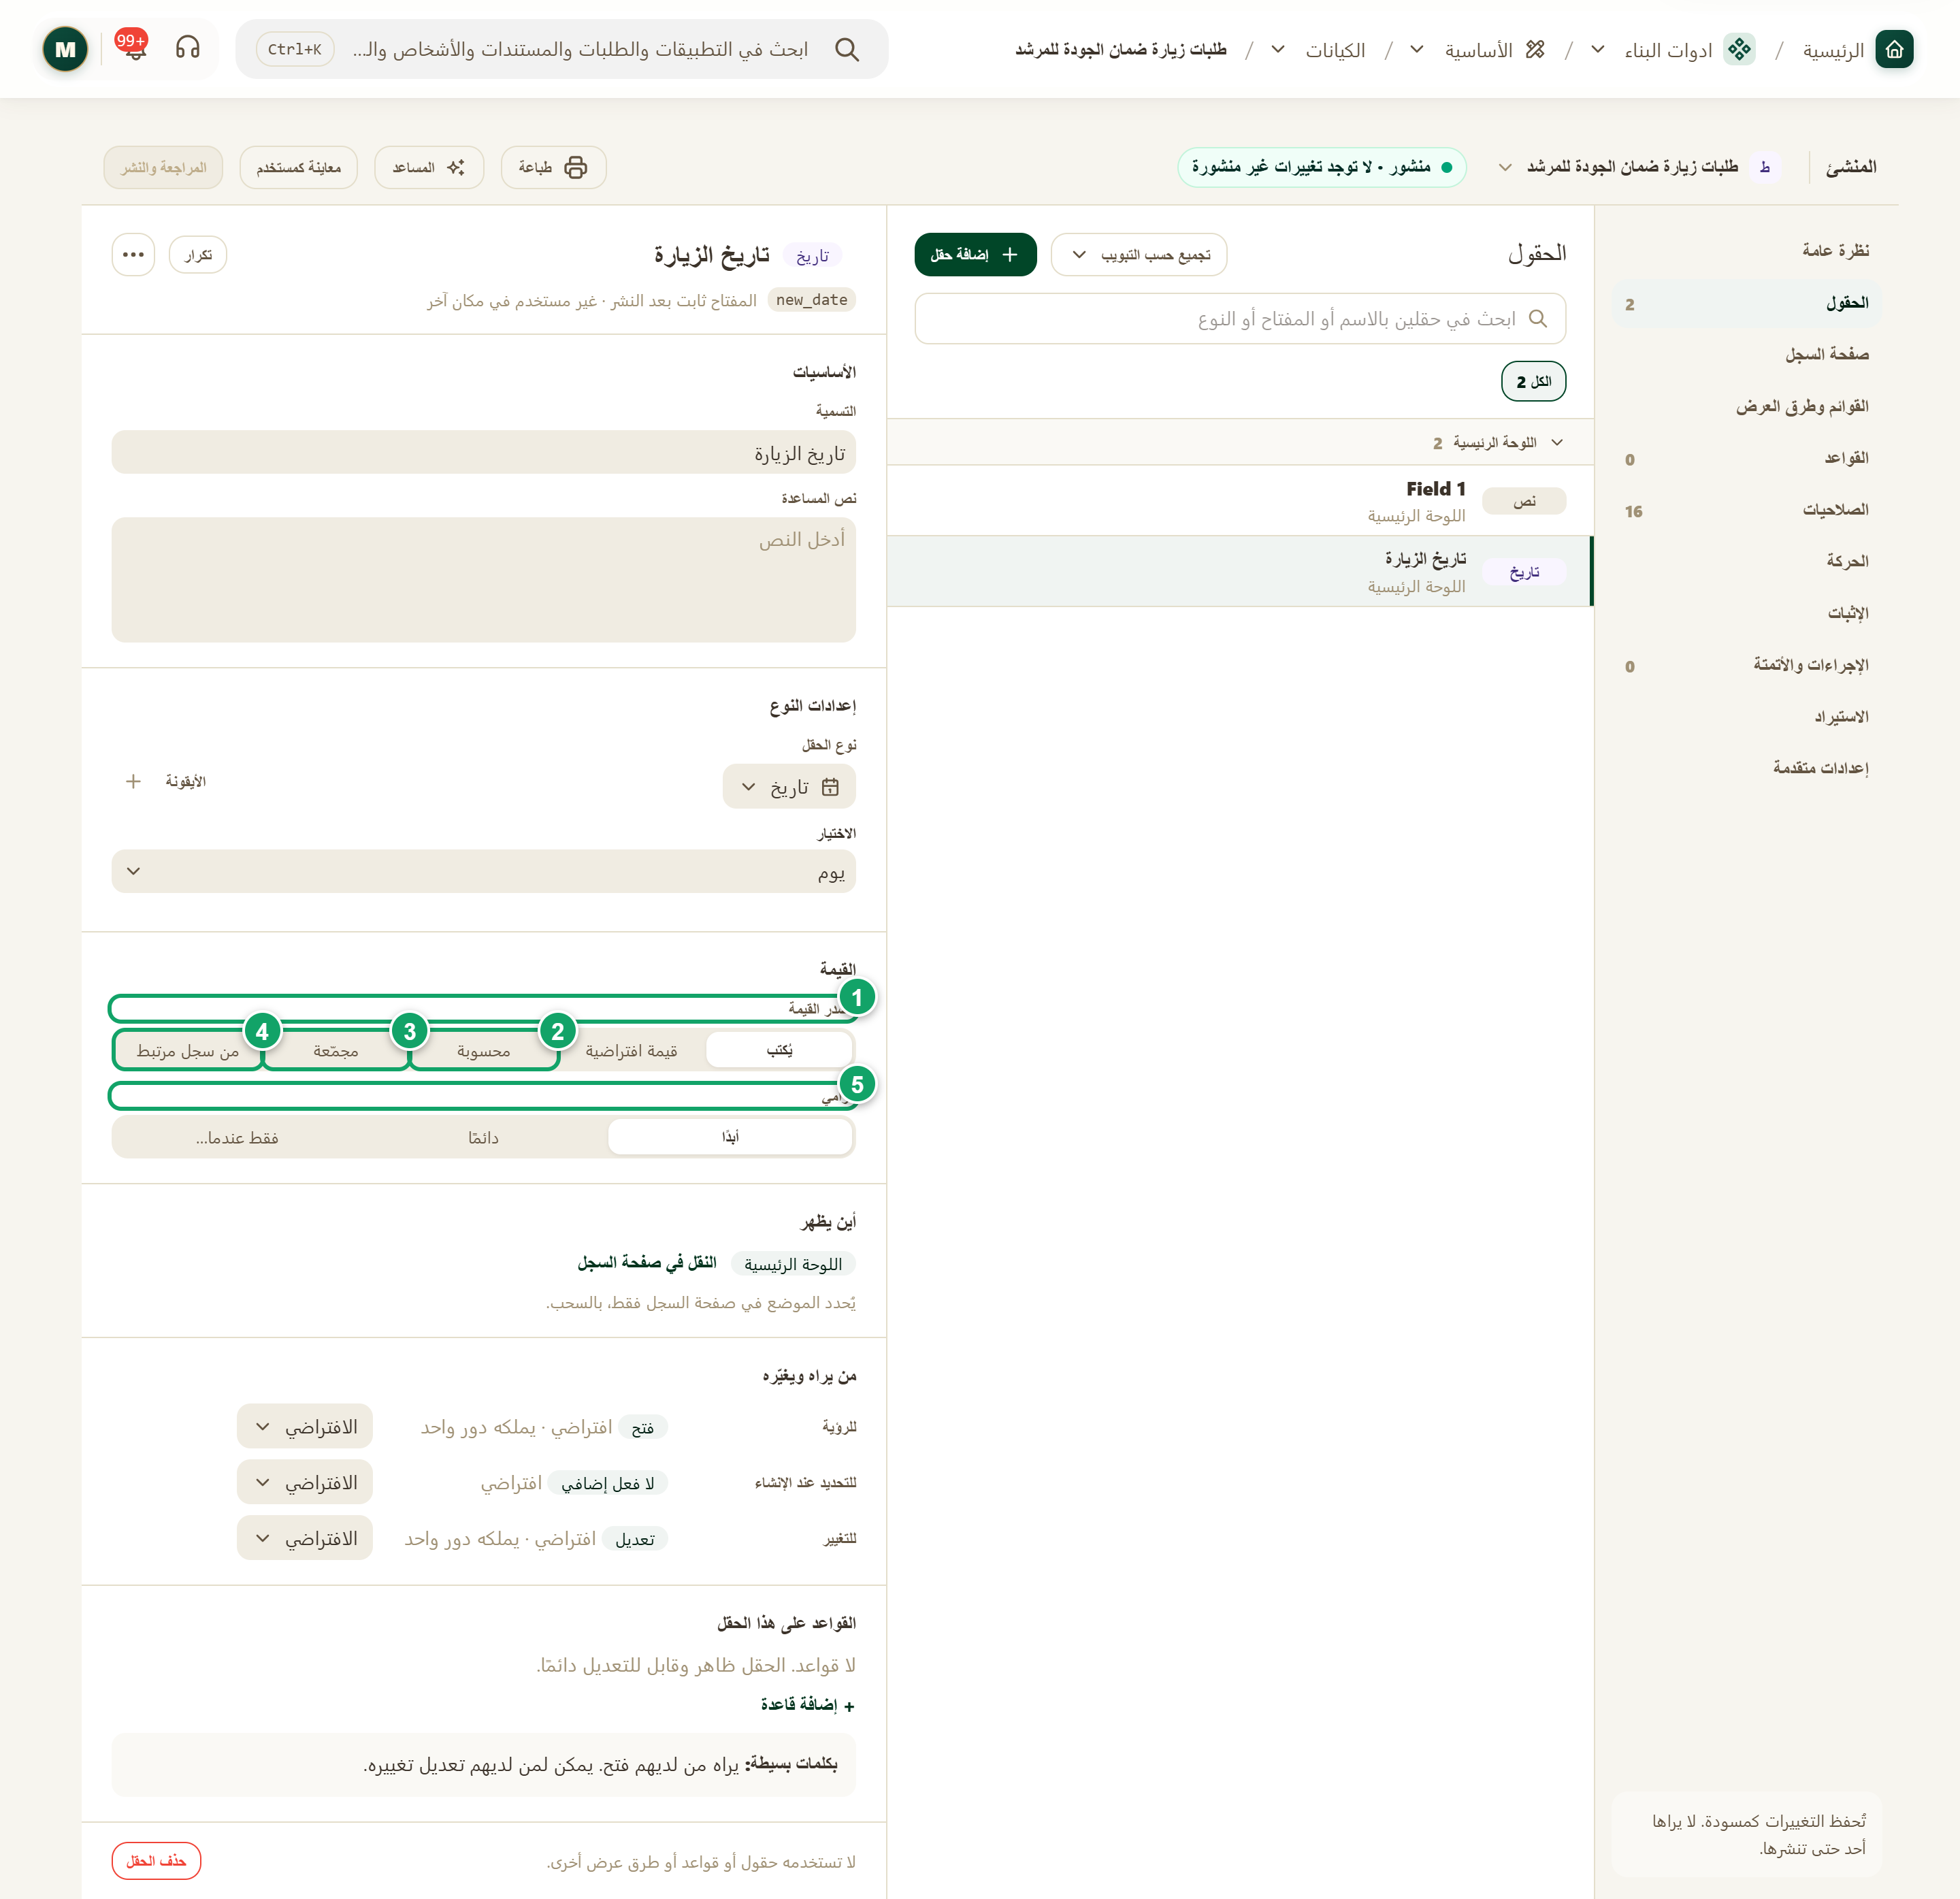
\includegraphics[width=0.95\linewidth,height=0.72\textheight,keepaspectratio]{figures/screens/ch06-ws-value-source-ar.png}
\caption{إعداد «مصدر القيمة» في لوحة حقل تاريخ}
\label{fig:builder-field-values-screen}
\shotnote{تعرض الصورة إعدادات حقل «تاريخ الزيارة» في النوع الاختباري، وقد ظهر فيها قسم «القيمة» بخياراته. ويبيّن ذلك أن مصدر القيمة وإلزامها يُضبطان في مكان واحد من لوحة الحقل. ① «مصدر القيمة». ② «محسوبة»: القيمة ناتج صيغة. ③ «مجمّعة»: القيمة من السجلات المرتبطة. ④ «من سجل مرتبط»: القيمة من حقل في سجل مرتبط. ⑤ «إلزامي»: متى يُمنع الحفظ إذا بقي الحقل فارغاً.}
\end{figure}

\begin{table}[H]
\centering
\caption{خيارات «مصدر القيمة»}
\label{tab:builder-field-values-sources}
\begin{tabularx}{\linewidth}{R{3.6cm} Y}
\rcHeaderRow
\thh{الخيار} & \thh{متى تستخدمه}\\
يُكتب & يكتب المستخدم القيمة بنفسه. وهو الخيار المعتاد لمعظم الحقول.\\
قيمة افتراضية & تبدأ القيمة بقيمة تحددها، ويستطيع المستخدم تغييرها، مثل حالة أولية أو تاريخ اليوم.\\
محسوبة & تُحسب القيمة بصيغة من حقول السجل نفسه أو السجلات المرتبطة به، مثل الكمية مضروبة في السعر. وتحدد في «التحديث التلقائي» هل تُعاد الحسبة عند تغيّر بيانات السجل فقط أم يومياً أو أسبوعياً أو شهرياً.\\
مجمّعة & تُجمع القيمة من السجلات التي ترتبط بهذا السجل أو من المهام المرتبطة به: عددها، أو مجموع حقل فيها، أو متوسطه، أو أقله أو أعلاه، أو أقدم تاريخ وأحدثه.\\
من سجل مرتبط & تُعرض قيمة حقل من سجل مرتبط، مثل محافظة الفرع، وتتحدث تلقائياً عند تغيّرها هناك.\\
\end{tabularx}
\end{table}

\subsection{بناء قيمة مجمّعة}

عندما تختار «مجمّعة» يظهر محرر يقودك خطوة بخطوة. تبدأ بـ«التجميع من» فتختار السجلات التي ترتبط بهذا السجل، ثم تختار في «الحساب» العملية، مثل «العدد» أو «المجموع» أو «المتوسط». وتستطيع أن تضيّق السجلات بشروط في «تضمين السجلات التي»، وأن تقسم النتيجة على عدد السجلات لتعرضها نسبة مئوية. وتعرض المعاينة النتيجة على سجل نموذجي، ثم تضغط «استخدام هذا التجميع».

\subsection{عرض قيمة من سجل مرتبط}

عندما تختار «من سجل مرتبط» تظهر نافذة «من أين تأتي القيمة؟»، فتختار العلاقة ثم الحقل الذي تريد عرضه. وإذا كان للسجل أكثر من سجل مرتبط، فتحدد في «الحساب» هل تعرض أولها أو قائمة بقيمها أو عددها أو مجموعها. وتحدد أيضاً ما يظهر عندما لا يوجد سجل مرتبط: حقل فارغ أو نص تكتبه. ولا تُحسب السجلات المؤرشفة، ولا يمكن جعل هذا الحقل إلزامياً؛ فاجعل حقل العلاقة نفسه إلزامياً بدلاً منه.

\subsection{إلزامي: أبدًا أو دائمًا أو فقط عندما}

يحدد إعداد «إلزامي» متى يُمنع حفظ السجل إذا بقي الحقل فارغاً: «أبدًا»، أو «دائمًا»، أو «فقط عندما…» لحالة معينة. والخيار الأخير ينقلك إلى «القواعد» لتبني قاعدة «إلزام» بشرطها. ولا يتاح هذا الإعداد في الحقول المحسوبة والمرتبطة، لأن المستخدم لا يكتب قيمتها.

\begin{figure}[H]
\centering
\begin{tikzpicture}[node distance=0.5cm]
\node[stepBox] (a) {\RL{اختيار مجمّعة}};
\node[stepBox,below=of a] (b) {\RL{التجميع من}};
\node[stepBox,below=of b] (c) {\RL{الحساب}};
\node[stepBox,below=of c] (d) {\RL{تضمين السجلات التي}};
\node[stepBox,below=of d] (e) {\RL{المعاينة على سجل}};
\node[stepBox,below=of e] (f) {\RL{استخدام هذا التجميع}};
\draw[flowsTo] (a) -- (b);
\draw[flowsTo] (b) -- (c);
\draw[flowsTo] (c) -- (d);
\draw[flowsTo] (d) -- (e);
\draw[flowsTo] (e) -- (f);
\end{tikzpicture}
\rclegend
\caption{بناء قيمة مجمّعة}
\label{fig:builder-field-values-flow}
\shotnote{يتبع المخطط ترتيب المحرر نفسه: تختار السجلات أولاً لأن العمليات المتاحة تعتمد على حقولها، ثم الحساب، ثم الشروط التي تضيّقها. وتأتي المعاينة قبل الحفظ لترى الرقم على سجل حقيقي، فتكتشف خطأ الشرط أو العملية قبل أن يراه الفريق.}
\end{figure}

\subsection{خطوات العمل والتحقق}
\begin{enumerate}
\item أضف حقلاً من النوع المناسب للنتيجة، مثل «رقم» للعدد أو المجموع، ثم افتح «القيمة» واختر «مصدر القيمة».
\item لقيمة محسوبة، اختر «محسوبة» واكتب الصيغة في المحرر، ثم اختر «التحديث التلقائي» المناسب.
\item لقيمة مجمّعة، اتبع المحرر من «التجميع من» إلى «استخدام هذا التجميع».
\item لقيمة من سجل مرتبط، تأكد أن حقل «علاقة» موجود، ثم اختر «من سجل مرتبط» وحدد العلاقة والحقل.
\item انشر التغييرات، ثم افتح سجلاً مرتبطاً بسجلات أخرى وقارن القيمة بما تتوقعه.
\end{enumerate}

\textbf{تحقق ومعالجة المشكلة:} يجب أن تظهر القيمة دون أن يكتبها أحد، وأن تتغير عندما تتغير مصادرها. فإذا ظهر في «قبل النشر» «لا يمكن حساب» متبوعاً باسم الحقل، فالصيغة تشير إلى حقل غير موجود؛ اضغط «إصلاح المعادلة» واختر الحقل الصحيح. وإذا اخترت «يُكتب» لحقل مرتبط، فستبقى قيمه الحالية لكنها لن تتحدث بعد ذلك.

\clearpage
\section{حقل الحالة وقواعد دورة الحياة}
\label{sec:builder-feature-lifecycle}

حقل «الحالة» يتبع مراحل العمل في قالب حالات، مثل «جديد» ثم «قيد المراجعة» ثم «معتمد». وتضيف إليه «قواعد دورة الحياة» ضوابط: متى يُسمح بالانتقال من حالة إلى أخرى، ومن لا يحق له تنفيذه، وما الحقول التي تُضبط تلقائياً عند الانتقال، وهل يُقفل السجل في حالة معينة. فلا يعتمد الالتزام بالإجراء على تذكّر الموظفين.

\textbf{المسار ومن يستخدمه:} «المنشئ» ← «الحقول» ← اختر حقل الحالة ← «قواعد دورة الحياة». تحتاج القواعد إلى «قالب ثابت» في إعدادات الحقل، ولا تتاح في أنواع السجلات المدمجة. أما قوالب الحالات نفسها فيشرحها فصل المهام في الصفحة \ref{sec:tasks-feature-statuses}.

\begin{rcnote}[مثال: شركة الأفق]
يجعل المسؤول الانتقال إلى «معتمد» في «طلبات الزيارة» ممنوعاً على مقدّم الطلب نفسه، فلا يعتمد عمر حداد طلبه. ويضيف أثراً يكتب تاريخ الاعتماد واسم من اعتمد، ثم يقفل الطلب المعتمد فلا تتغير بياناته بعد أن تعتمده سارة الخطيب.
\end{rcnote}

\begin{table}[H]
\centering
\caption{ما تضبطه لكل انتقال}
\label{tab:builder-lifecycle-transitions}
\begin{tabularx}{\linewidth}{R{3.6cm} Y}
\rcHeaderRow
\thh{الإعداد} & \thh{المعنى}\\
فقط عندما & شرط يجب أن يتحقق قبل الانتقال، مثل وجود تاريخ للزيارة.\\
الرسالة عند المنع & النص الذي يراه المستخدم إذا لم يتحقق الشرط، فيعرف ما ينقصه.\\
لا يمكن أن ينفّذه الأعضاء المذكورون في & حقول أعضاء في السجل لا يحق لأصحابها تنفيذ الانتقال، مثل مقدّم الطلب.\\
عند تنفيذ الانتقال & آثار تُضبط في الحفظ نفسه: «اضبط» حقلاً على «الآن» أو «العضو الحالي» أو قيمة ثابتة أو تعبير، أو «امسح» قيمته. وتُكتب هذه الحقول حتى لو كان السجل مقفلاً.\\
\end{tabularx}
\end{table}

\begin{table}[H]
\centering
\caption{ما تضبطه لكل حالة}
\label{tab:builder-lifecycle-states}
\begin{tabularx}{\linewidth}{R{3.6cm} Y}
\rcHeaderRow
\thh{الإعداد} & \thh{المعنى}\\
التعديل & «غير مقفل»، أو «مقفل»، أو «مقفل باستثناء» حقول تبقى قابلة للتعديل.\\
منع الحذف & يمنع حذف السجل ما دام في هذه الحالة.\\
قفل السجلات التي تشير إليه & يقفل أيضاً السجلات المرتبطة به، مثل بنود طلب معتمد.\\
تجميد إصدار عند الدخول & يحفظ نسخة من السجل باسم تحدده عند دخوله الحالة، لتعود إليها لاحقاً.\\
\end{tabularx}
\end{table}

\begin{rcwarn}[الحالة تتغير بالانتقالات فقط]
عند تفعيل «لا تتغير الحالة إلا عبر الانتقالات» لا تستطيع النماذج أو الاستيراد أو الأتمتة أن تضبط الحالة مباشرة، ويبدأ كل سجل جديد من الحالة الأولى. فإذا كانت لديك أتمتة تغيّر الحالة، فراجعها قبل تفعيل هذا الخيار.
\end{rcwarn}

\begin{figure}[H]
\centering
\begin{tikzpicture}[node distance=0.5cm]
\node[stepBox] (a) {\RL{قالب ثابت للحالة}};
\node[stepBox,below=of a] (b) {\RL{شروط الانتقالات}};
\node[stepBox,below=of b] (c) {\RL{من لا ينفّذ الانتقال}};
\node[stepBox,below=of c] (d) {\RL{آثار الانتقال}};
\node[stepBox,below=of d] (e) {\RL{القفل في كل حالة}};
\draw[flowsTo] (a) -- (b);
\draw[flowsTo] (b) -- (c);
\draw[flowsTo] (c) -- (d);
\draw[flowsTo] (d) -- (e);
\end{tikzpicture}
\rclegend
\caption{ضبط دورة حياة السجل}
\label{fig:builder-lifecycle-flow}
\shotnote{يبدأ المخطط بالقالب الثابت لأن القواعد كلها تُبنى على انتقالاته، فلا تظهر دونه. ثم يضبط كل انتقال على حدة، وينتهي بالقفل لأنه يحمي السجل بعد وصوله إلى الحالة، فيصبح الترتيب: متى ينتقل السجل، ومن ينقله، وماذا يحدث بعد ذلك.}
\end{figure}

\subsection{خطوات العمل والتحقق}
\begin{enumerate}
\item افتح حقل الحالة في «الحقول»، واختر في «إعدادات النوع» «قالب ثابت» وقالب الحالات المناسب.
\item افتح «قواعد دورة الحياة»، واختر الانتقال الذي تريد ضبطه، وأضف شرطه في «فقط عندما» ورسالته في «الرسالة عند المنع».
\item حدد في «لا يمكن أن ينفّذه الأعضاء المذكورون في» حقل مقدّم الطلب إن كان لا يحق له اعتماد طلبه.
\item أضف في «عند تنفيذ الانتقال» أثراً يكتب التاريخ أو العضو الحالي، ثم حدد قفل التعديل للحالة النهائية.
\item انشر التغييرات، وجرّب الانتقال بسجل تجريبي مرة بشرط ناقص ومرة بشرط مكتمل.
\end{enumerate}

\textbf{تحقق ومعالجة المشكلة:} يجب أن يُمنع الانتقال مع رسالتك عندما ينقص الشرط، وأن يتم ويكتب الحقول المحددة عندما يكتمل. فإذا لم تظهر «قواعد دورة الحياة»، فاختر «قالب ثابت» أولاً؛ وإذا كان النوع مدمجاً في النظام، فهذه القواعد غير متاحة له.

\clearpage
\section{صفحة السجل}
\label{sec:builder-feature-record-page}

صفحة السجل هي ما يراه المستخدم عندما يفتح سجلاً واحداً. ويرتّب قسم «صفحة السجل» الحقول في تبويبات وأقسام، فتظهر المعلومات المترابطة معاً بدلاً من قائمة طويلة واحدة. ويمكنك أن تضيف كتلاً في أعلى التبويب الأول، وقوائم بالسجلات المرتبطة.

\textbf{المسار ومن يستخدمه:} نوع السجلات ← «صفحة السجل». يستخدمه من يبني النوع بعد إضافة حقوله.

\begin{rcnote}[مثال: شركة الأفق]
يجعل مسؤول النظام لصفحة طلب الزيارة تبويبين: «الطلب» للفرع والموعد والغرض، و«المراجعة» لملاحظات سارة الخطيب وقرارها، فيجد عمر حداد ما يخصه في التبويب الأول. ويبدأ بإنشاء التبويبين من ② ثم يسحب الحقول إليهما.
\end{rcnote}

\begin{figure}[H]
\centering
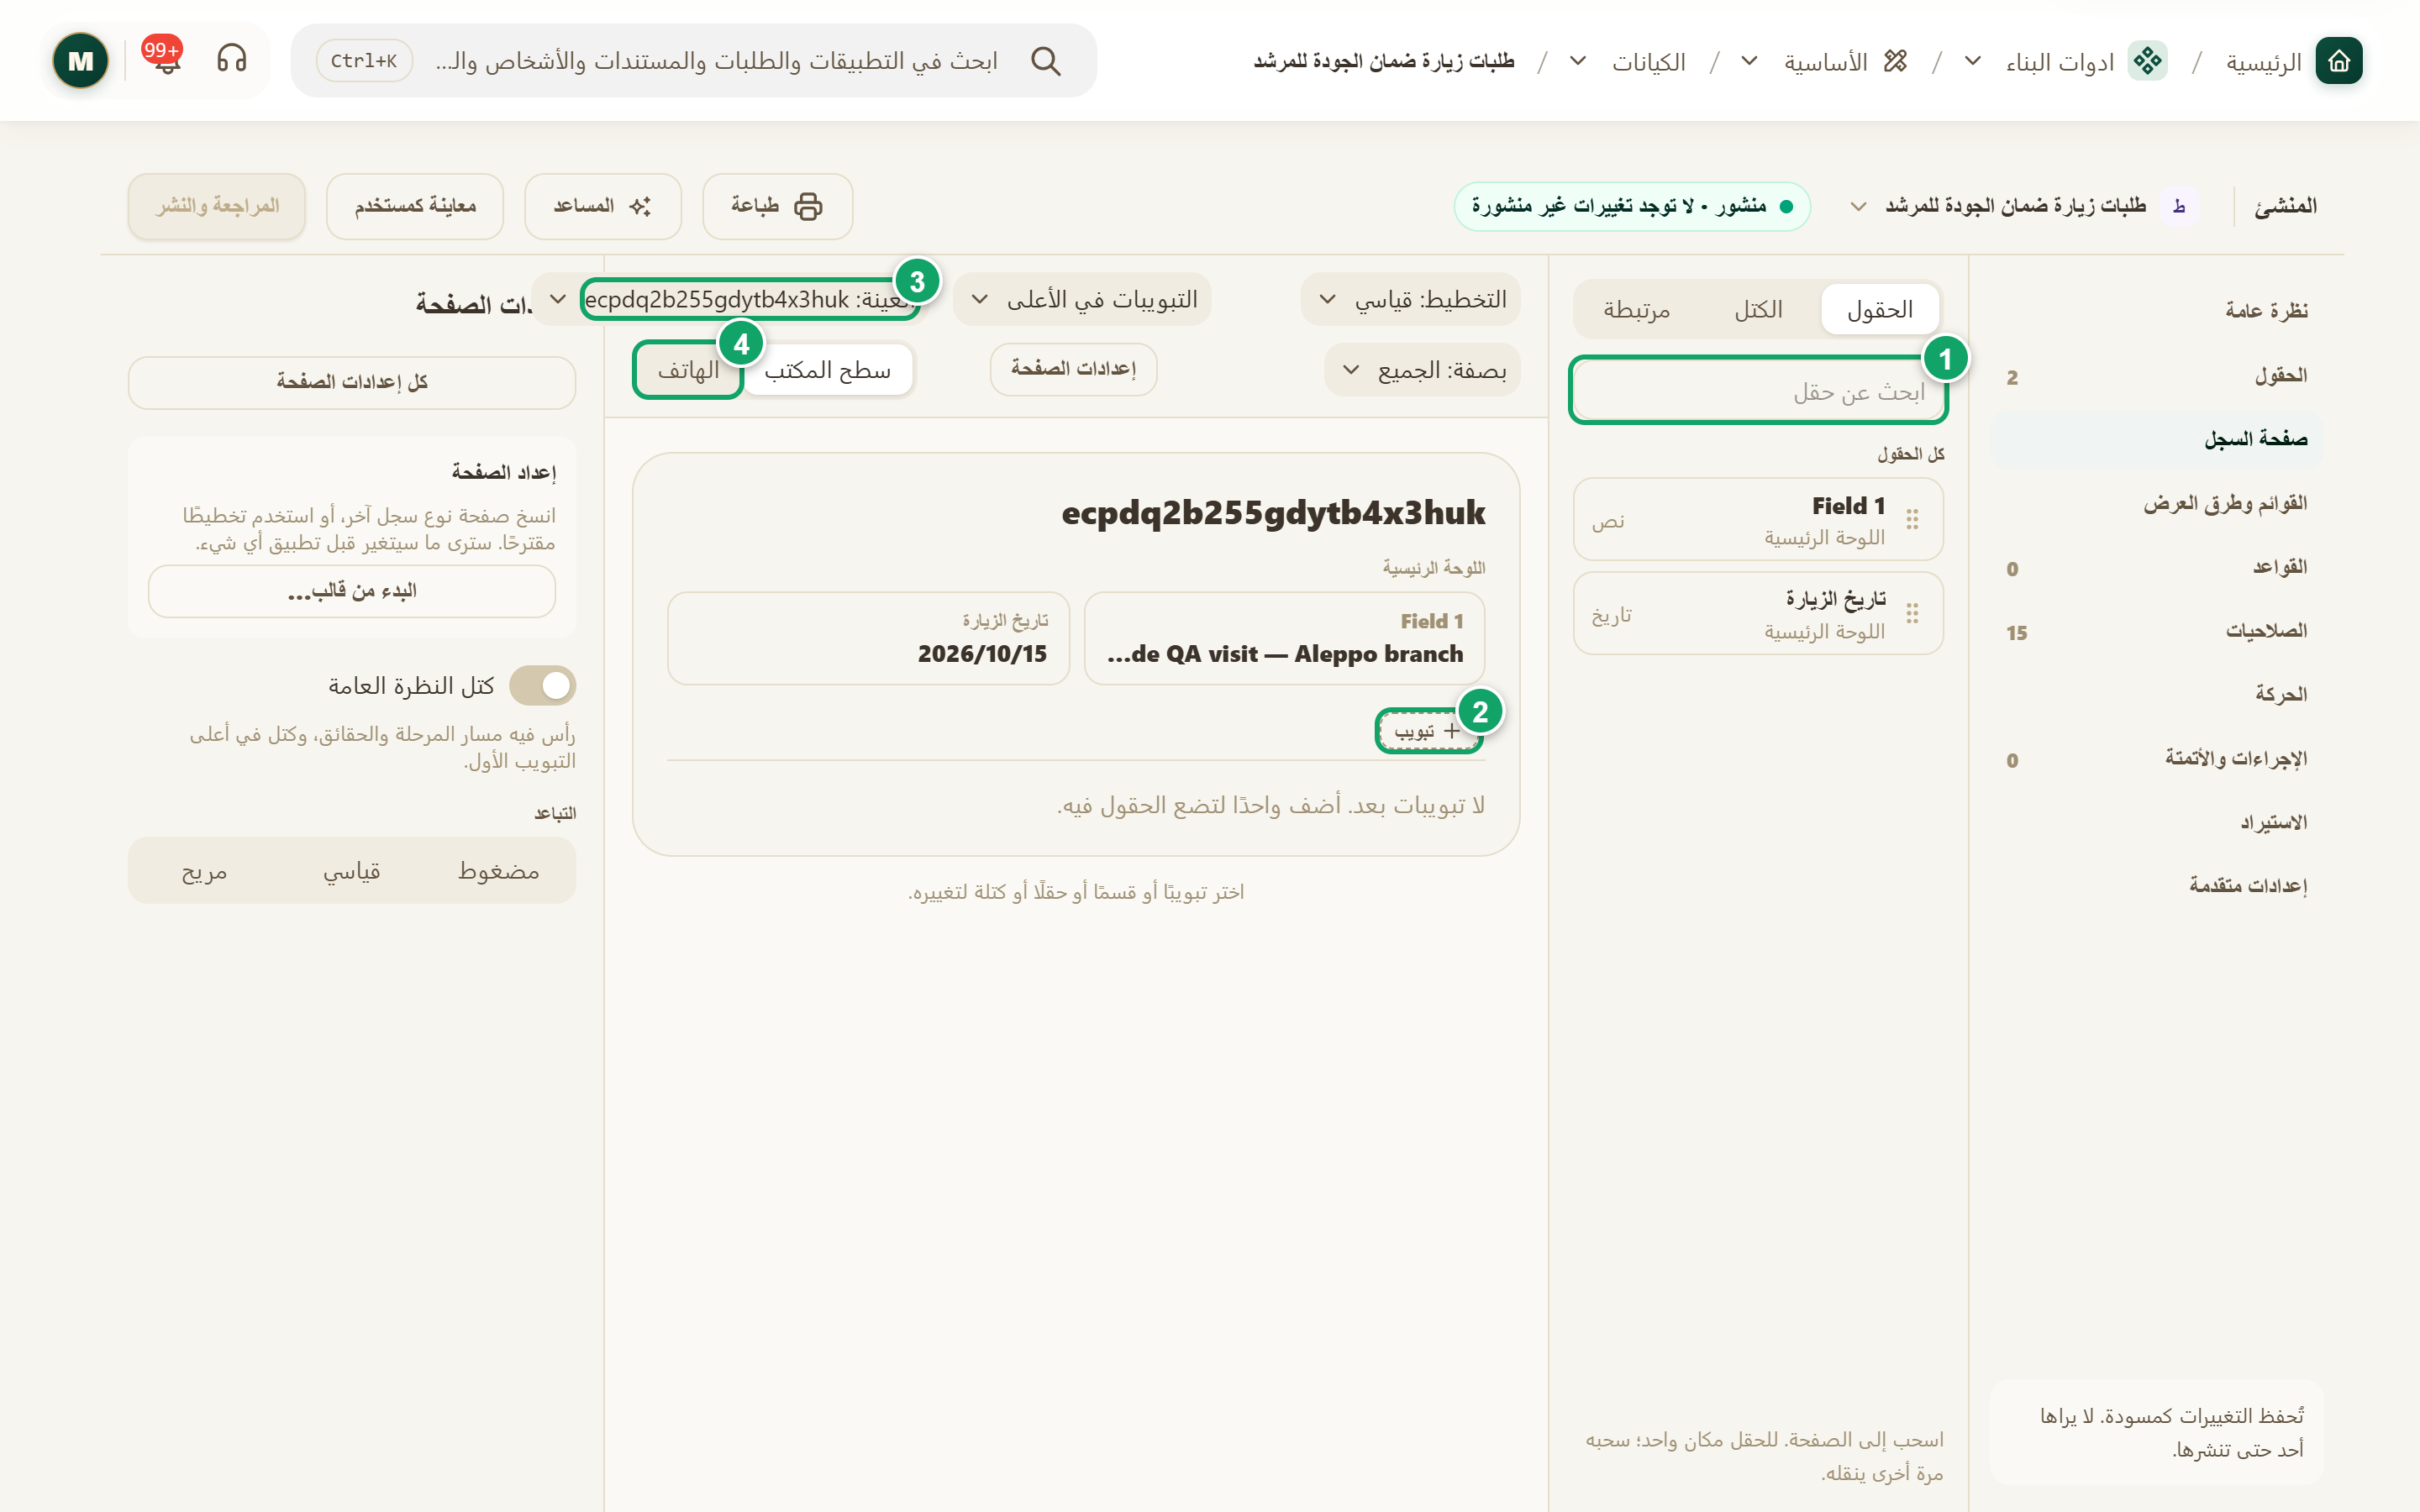
\includegraphics[width=0.95\linewidth,height=0.72\textheight,keepaspectratio]{figures/screens/ch06-ws-record-page-ar.png}
\caption{قسم «صفحة السجل» مع معاينة بسجل حقيقي}
\label{fig:builder-record-page-screen}
\shotnote{يعرض القسم أجزاء الصفحة على جانب، والصفحة نفسها في الوسط بقيم سجل اختباري، فترى أثر الترتيب قبل النشر. ① «ابحث عن حقل»: تجد الحقل الذي تريد سحبه إلى الصفحة. ② «تبويب»: يضيف تبويباً تضع فيه الأقسام والحقول. ③ «العينة»: السجل الذي تُعاين به الصفحة. ④ «الهاتف»: يعرض الصفحة كما تظهر على الشاشة الصغيرة.}
\end{figure}


\begin{table}[H]
\centering
\caption{ما الذي تجده هنا؟}
\label{tab:builder-record-page-data}
\begin{tabularx}{\linewidth}{R{3.6cm} Y}
\rcHeaderRow
\thh{القسم} & \thh{المحتوى والإجراء}\\
التبويبات والأقسام & أنشئ «تبويب جديد» أو «قسم جديد»، ثم اسحب الحقول إليها. للحقل مكان واحد في الصفحة، وسحبه مرة أخرى ينقله.\\
أجزاء الصفحة & تجمع «كل الحقول» و«الكتل» والقوائم «المرتبطة»، وتعرض الحقول التي «ليست في الصفحة بعد».\\
التخطيط والرأس & يختار شكل الصفحة: تبويبات أو قائمة أقسام، مع إعدادات الرأس وكتل النظرة العامة.\\
المعاينة & تعرض الصفحة بعينة من سجل حقيقي، كما يراها دور معيّن، على سطح المكتب أو الهاتف.\\
\end{tabularx}
\end{table}

\begin{figure}[H]
\centering
\begin{tikzpicture}[node distance=0.5cm]
\node[entity] (page) {\RL{صفحة السجل}};
\node[entity,below=0.7cm of page] (tab) {\RL{تبويب}};
\node[entity,below=0.7cm of tab] (section) {\RL{قسم}};
\node[entity,below=0.7cm of section] (field) {\RL{حقل}};
\draw[dependsOn] (page) -- (tab);
\draw[dependsOn] (tab) -- (section);
\draw[dependsOn] (section) -- (field);
\end{tikzpicture}
\rclegend
\caption{كيف تُرتّب الصفحة}
\label{fig:builder-record-page-tree}
\shotnote{يوضّح الشكل تدرّج الترتيب: تضم الصفحة تبويبات، ويضم كل تبويب أقساماً، ويضم كل قسم حقولاً. لذلك تنشئ التبويب والقسم أولاً ثم تسحب الحقول إليهما، والحقل الذي لا تضعه في أي قسم يبقى محفوظاً لكنه لا يظهر في الصفحة.}
\end{figure}

\subsection{خطوات العمل والتحقق}
\begin{enumerate}
\item افتح نوع السجلات واختر «صفحة السجل».
\item أنشئ التبويبات التي يحتاجها العمل، ثم أضف قسماً أو أكثر في كل تبويب.
\item اسحب كل حقل من «أجزاء الصفحة» إلى القسم المناسب، وراجع «ليست في الصفحة بعد» حتى لا يبقى حقل مهم خارج الصفحة.
\item غيّر حجم المعاينة إلى «الهاتف» لتتأكد من أن الصفحة واضحة على الشاشة الصغيرة.
\end{enumerate}

\textbf{تحقق ومعالجة المشكلة:} يجب أن تعرض المعاينة الحقول في التبويبات والأقسام التي اخترتها. فإذا لم يظهر حقل، فابحث عنه في «ليست في الصفحة بعد» واسحبه إلى قسم؛ وإذا ظهرت رسالة بأن الحقل موضوع في تبويب غير موجود، فانقله إلى تبويب قائم.

\clearpage
\section{كتل النظرة العامة والتخطيطات}
\label{sec:builder-feature-record-page-blocks}

إلى جانب الحقول، يمكن أن تبدأ صفحة السجل بملخص يعرض أهم ما فيه: مسار المراحل، وأرقام رئيسية، وما يحتاج إلى متابعة. وتُبنى هذه الملخصات من «كتل النظرة العامة» التي تظهر أعلى التبويب الأول. أما «التخطيطات» فنسخ محفوظة من ترتيب الصفحة، تختار بينها حسب قيمة في السجل، فيرى كل نوع من السجلات الترتيب الأنسب له.

\textbf{المسار ومن يستخدمه:} «المنشئ» ← «صفحة السجل» ← «إعدادات الصفحة» لتفعيل كتل النظرة العامة، ثم «أجزاء الصفحة» ← «الكتل» لإضافتها. والتخطيطات من «إدارة التخطيطات…». يستخدمه من يبني النوع بعد أن تستقر حقوله.

\begin{rcnote}[مثال: شركة الأفق]
يضيف المسؤول إلى صفحة «طلبات الزيارة» كتلة «مؤشرات» تعرض عدد أيام الطلب منذ إنشائه، وكتلة «يحتاج إلى متابعة» تنبّه سارة الخطيب إلى الطلب الذي مضى عليه أكثر من ثلاثة أيام دون مراجعة.
\end{rcnote}

\begin{figure}[H]
\centering
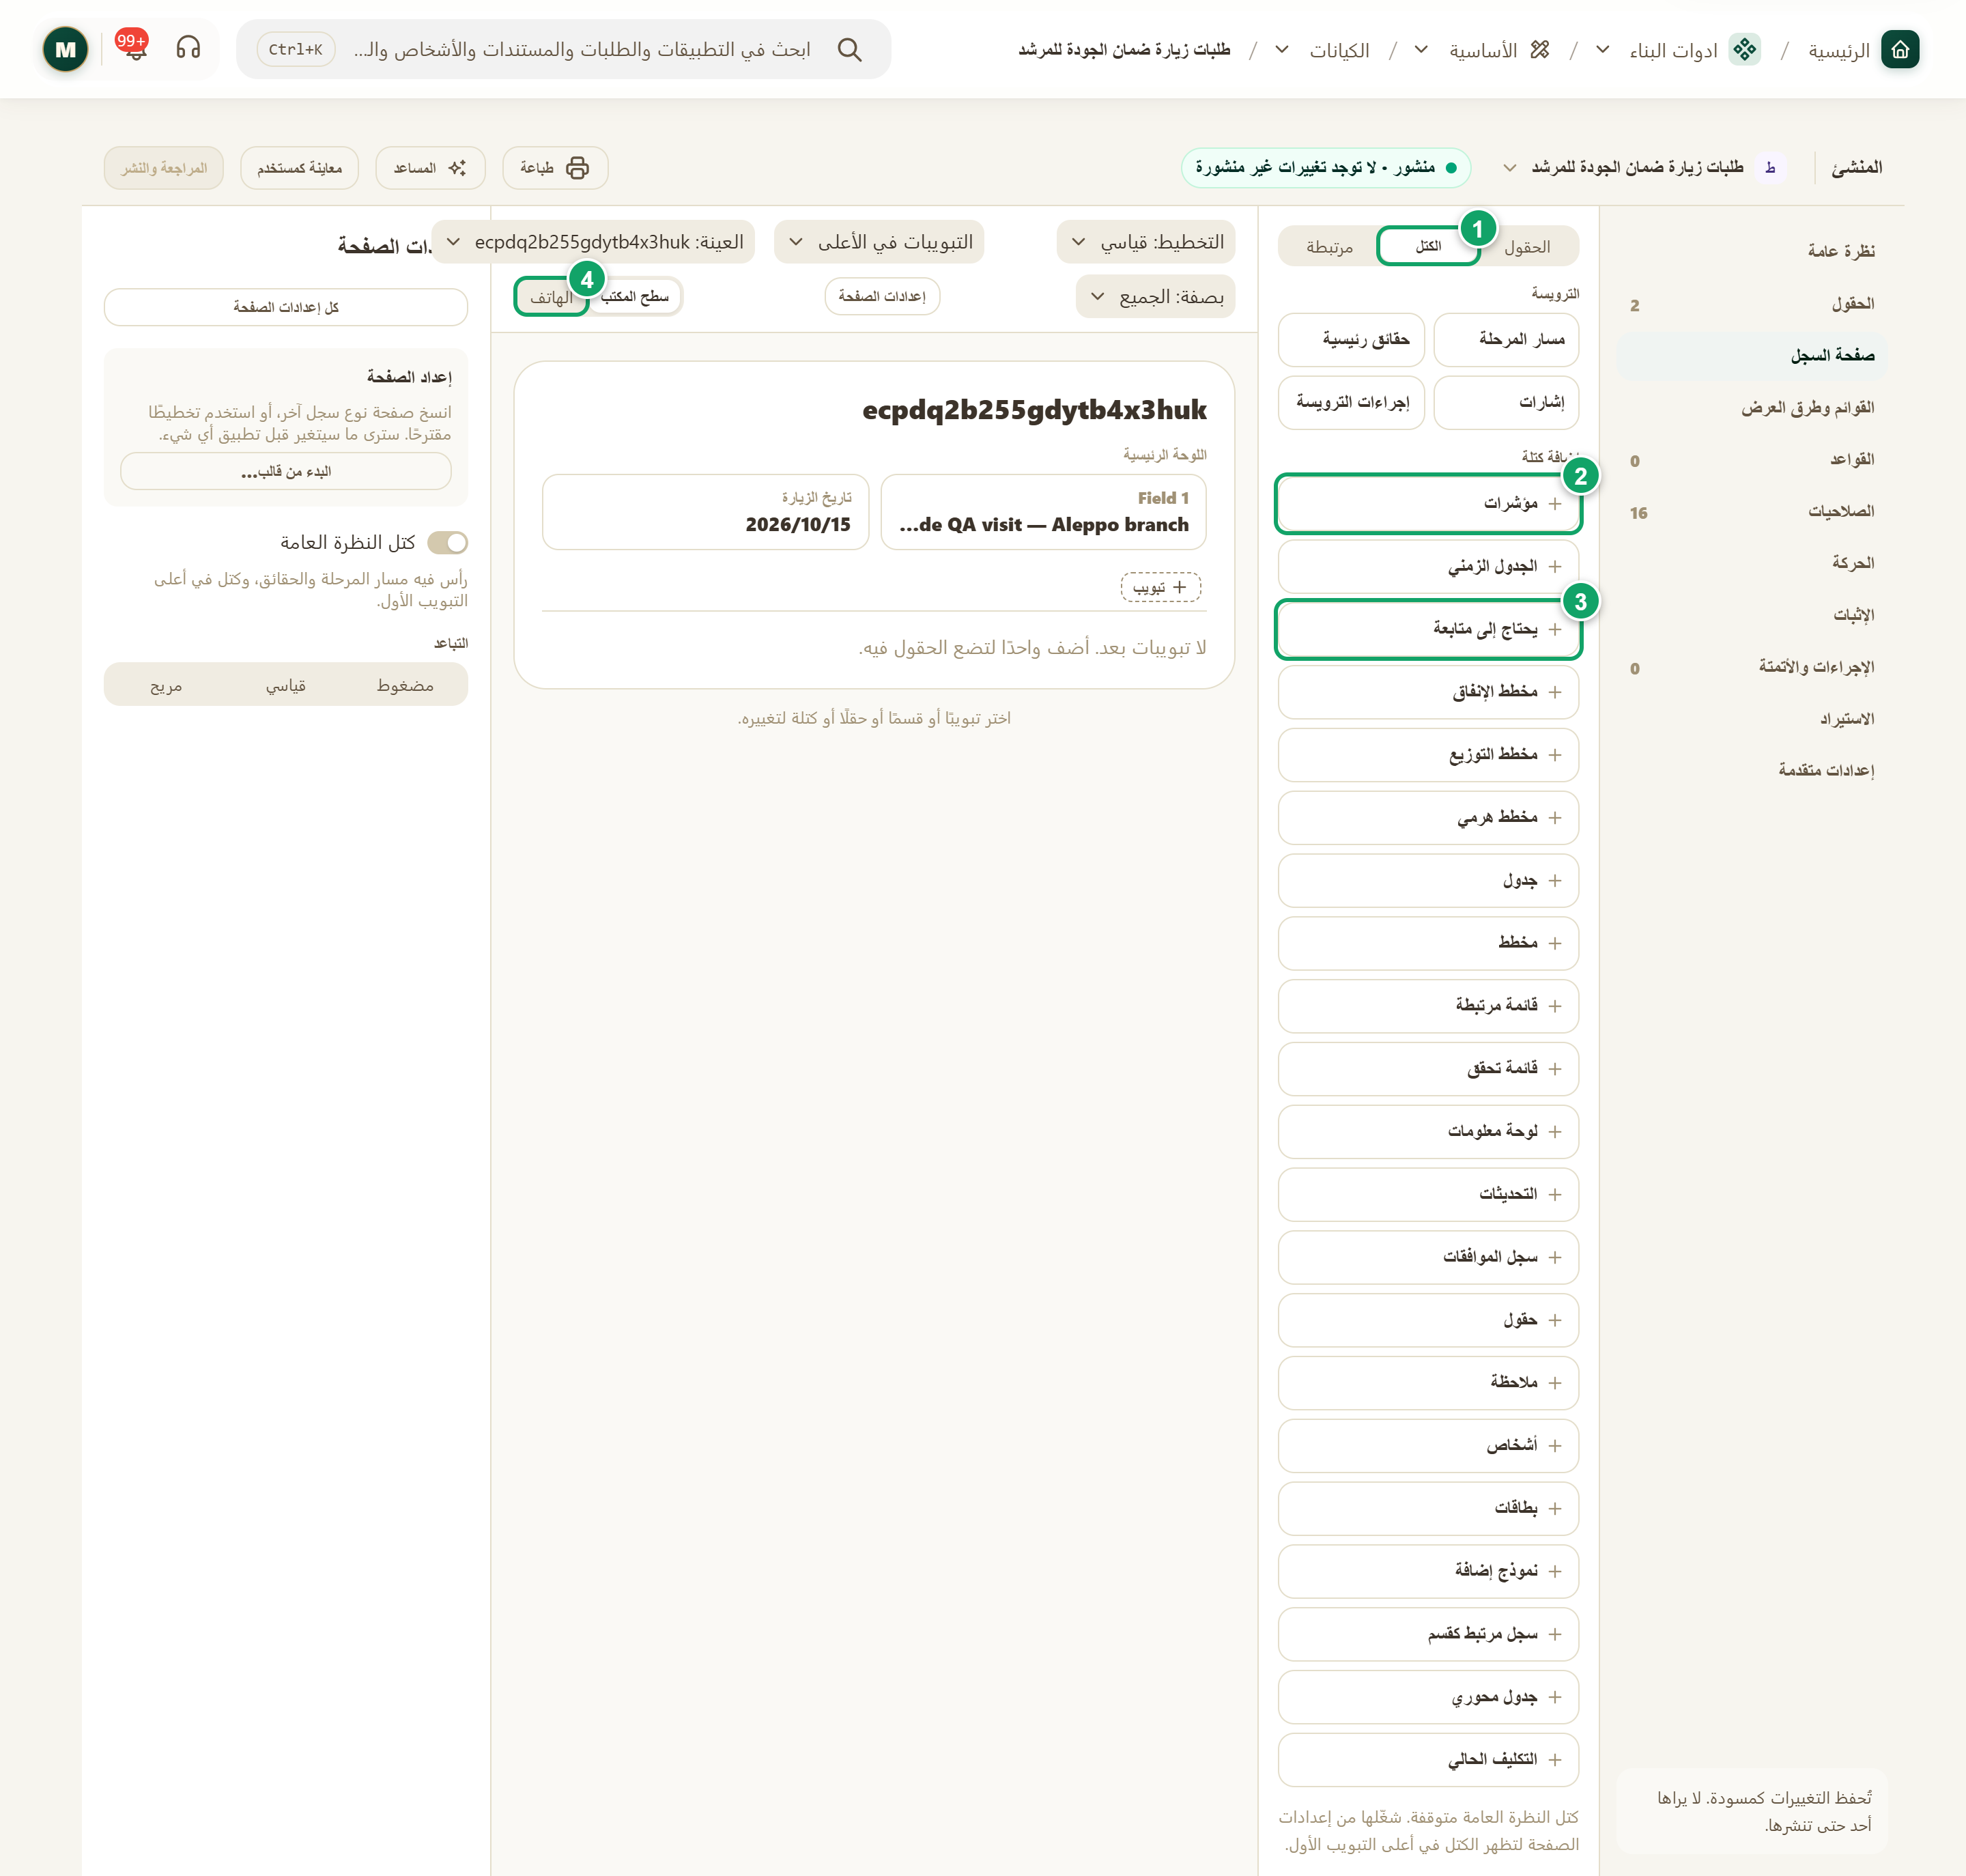
\includegraphics[width=0.95\linewidth,height=0.72\textheight,keepaspectratio]{figures/screens/ch06-ws-blocks-ar.png}
\caption{تبويب «الكتل» في «أجزاء الصفحة»}
\label{fig:builder-record-page-blocks-screen}
\shotnote{تعرض الصورة قسم «صفحة السجل» بعد فتح تبويب الكتل، وفيه كل الكتل التي يمكن وضعها أعلى التبويب الأول، والمعاينة إلى جانبها. ويفيدك ذلك في اختيار الكتلة ورؤية أثرها قبل النشر. ① «الكتل». ② «مؤشرات»: أرقام رئيسية عن السجل. ③ «يحتاج إلى متابعة»: تنبيهات بقواعد تحددها. ④ «الهاتف»: يعرض المعاينة بحجم شاشة الهاتف.}
\end{figure}

\begin{table}[H]
\centering
\caption{أجزاء الصفحة}
\label{tab:builder-record-page-blocks-parts}
\begin{tabularx}{\linewidth}{R{3.6cm} Y}
\rcHeaderRow
\thh{التبويب} & \thh{ما تضيفه منه}\\
الحقول & تسحب الحقل إلى مكانه في الصفحة. وتظهر الحقول غير الموضوعة في «ليست في الصفحة بعد»، والحقل يوجد في مكان واحد، فسحبه مرة أخرى ينقله.\\
الكتل & تختار كتلة لتضبطها، ثم تضيفها أعلى التبويب الأول.\\
مرتبطة & قوائم بالسجلات المرتبطة، وتوضع من حقل العلاقة في النوع المرتبط.\\
\end{tabularx}
\end{table}

\begin{table}[H]
\centering
\caption{أكثر الكتل استخداماً}
\label{tab:builder-record-page-blocks-kinds}
\begin{tabularx}{\linewidth}{R{3.6cm} Y}
\rcHeaderRow
\thh{الكتلة} & \thh{ما تعرضه}\\
مؤشرات & أرقاماً رئيسية، مثل نسبة الإنجاز، أو المستخدم من إجمالي، أو تأخر موعد.\\
يحتاج إلى متابعة & تنبيهات بقواعد تحددها، بدرجة «حرج» أو «تحذير» أو «معلومة»، مع عدد السجلات المطابقة أو قائمتها.\\
الجدول الزمني & المواعيد والمراحل من السجل والسجلات المرتبطة به على خط زمني.\\
قائمة مرتبطة وبطاقات & السجلات المرتبطة في جدول أو بطاقات داخل الصفحة.\\
سجل الموافقات والتحديثات & تاريخ الموافقات وآخر التحديثات على السجل.\\
ملاحظة وحقول وأشخاص & نصاً ثابتاً، أو مجموعة حقول، أو الأشخاص المرتبطين بالسجل.\\
مخطط ولوحة معلومات & رسماً بيانياً من بيانات السجل، أو لوحة معلومات جاهزة.\\
\end{tabularx}
\end{table}

\subsection{المعاينة والتخطيطات}

تعرض المعاينة الصفحة بسجل نموذجي من «العينة»، وتستطيع أن تراها «بصفة» دور معين، وبحجم «سطح المكتب» أو «الهاتف». أما «إدارة التخطيطات…» فتفتح نافذة «التخطيطات»: التخطيط يحفظ أنماط الأقسام وأعمدتها والمسافات والرأس وكتل النظرة العامة، أما التبويبات والأقسام ومواضع الحقول فمشتركة بين كل التخطيطات. وتحدد فيها التخطيط الافتراضي، أو تختار التخطيط من قيمة حقل في السجل.

\begin{figure}[H]
\centering
\begin{tikzpicture}[node distance=0.5cm]
\node[stepBox] (a) {\RL{تفعيل كتل النظرة العامة}};
\node[stepBox,below=of a] (b) {\RL{إضافة كتلة}};
\node[stepBox,below=of b] (c) {\RL{ضبط الكتلة وعرضها}};
\node[stepBox,below=of c] (d) {\RL{المعاينة بصفة دور}};
\node[stepBox,below=of d] (e) {\RL{المراجعة والنشر}};
\draw[flowsTo] (a) -- (b);
\draw[flowsTo] (b) -- (c);
\draw[flowsTo] (c) -- (d);
\draw[flowsTo] (d) -- (e);
\end{tikzpicture}
\rclegend
\caption{إضافة كتلة إلى صفحة السجل}
\label{fig:builder-record-page-blocks-flow}
\shotnote{يبدأ المخطط بتفعيل كتل النظرة العامة لأن تبويب «الكتل» لا يضيف شيئاً قبل ذلك. ثم تأتي المعاينة بصفة دور قبل النشر، لأن الكتلة قد تعرض أرقاماً من سجلات لا يحق لبعض الأدوار رؤيتها، فتتأكد مما يراه كل منهم.}
\end{figure}

\subsection{خطوات العمل والتحقق}
\begin{enumerate}
\item افتح «صفحة السجل»، ثم «إعدادات الصفحة»، وفعّل كتل النظرة العامة.
\item افتح «أجزاء الصفحة» ← «الكتل»، واختر الكتلة، ثم اضغط «إضافة كتلة».
\item اضبط الكتلة: العنوان والعرض («كامل العرض» أو «الثلثان» أو «الثلث») وما تعرضه، مثل قواعد «يحتاج إلى متابعة».
\item غيّر «بصفة» إلى دور آخر، و«حجم المعاينة» إلى «الهاتف»، وتأكد أن الصفحة واضحة في الحالتين، ثم انشر.
\end{enumerate}

\textbf{تحقق ومعالجة المشكلة:} يجب أن تظهر الكتلة أعلى التبويب الأول عند فتح سجل منشور. فإذا ظهر «كتل النظرة العامة متوقفة»، فاضغط «تشغيل كتل النظرة العامة» أولاً. وإذا كانت الكتلة فارغة، فجرّبها على سجل فيه البيانات التي تعتمد عليها.

\clearpage
\section{القوائم وطرق العرض}
\label{sec:builder-feature-lists}

يحدد قسم «القوائم وطرق العرض» كيف تظهر سجلات النوع معاً عندما يفتح المستخدم القائمة. فتختار طرق العرض التي يمكن التبديل بينها، مثل «جدول» أو «كانبان» أو «التقويم»، والأعمدة الظاهرة، والأرقام التي تلخّص القائمة في أعلاها. وتتيح بطاقة «الخلايا القابلة للتعديل» خيار «تعديل الخلايا في مكانها»، فيعدّل المستخدمون خلايا الجدول دون فتح كل سجل، بشرط أن تكون طرق عرض القوائم مفعّلة وأن يملكوا صلاحية تغيير الحقل.

\textbf{المسار ومن يستخدمه:} نوع السجلات ← «القوائم وطرق العرض». يستخدمه من يبني النوع، ويفيد كل من يتابع السجلات يومياً.

\begin{rcnote}[مثال: شركة الأفق]
يعرض مسؤول النظام طلبات الزيارة في «جدول» بأعمدة الرقم والفرع والموعد والحالة، ويضيف «التقويم» حسب موعد الزيارة، فترى سارة الخطيب زيارات الأسبوع في نظرة واحدة. ويبدأ بتفعيل المفتاح ① لاختيار الجدول والتقويم.
\end{rcnote}

\begin{figure}[H]
\centering
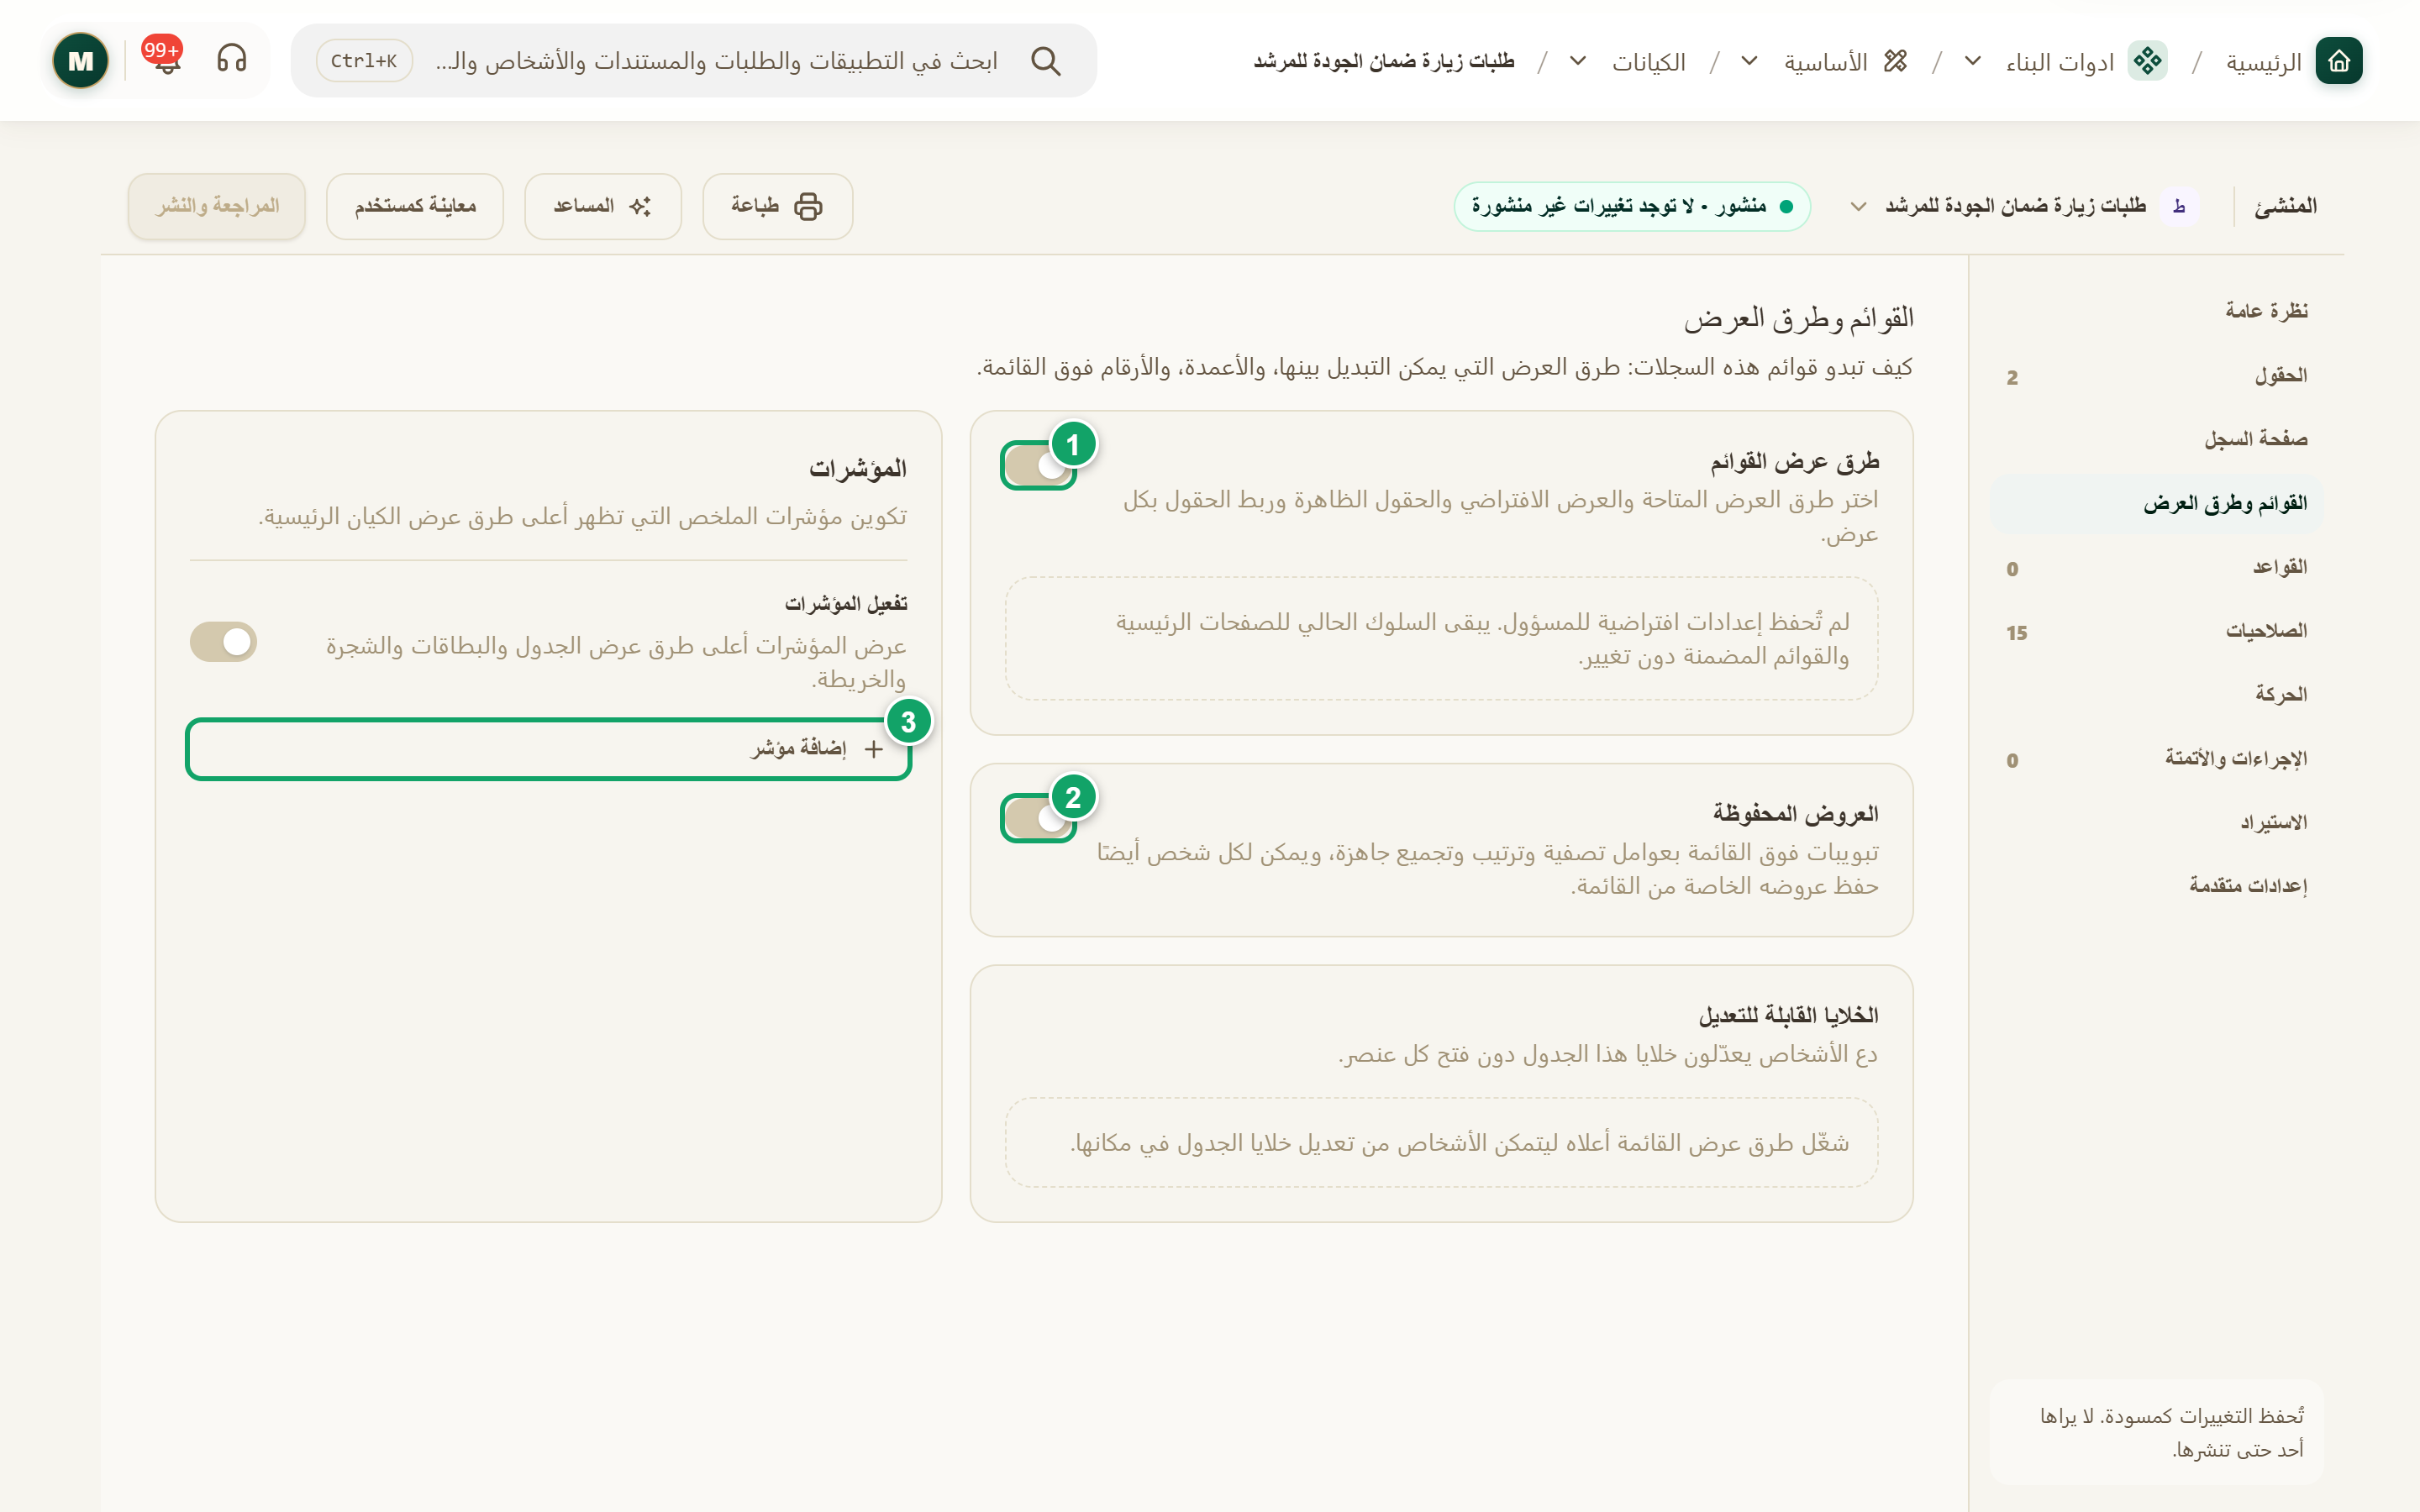
\includegraphics[width=0.95\linewidth,height=0.72\textheight,keepaspectratio]{figures/screens/ch06-ws-lists-ar.png}
\caption{قسم «القوائم وطرق العرض»}
\label{fig:builder-lists-screen}
\shotnote{يجمع القسم ما يتحكم في شكل قائمة السجلات. وكل المفاتيح متوقفة هنا، فتعمل القائمة بإعدادها الافتراضي. ① مفتاح «طرق عرض القوائم»: يتيح اختيار طرق العرض المتاحة والافتراضية والأعمدة. ② مفتاح «العروض المحفوظة»: يضيف تبويبات جاهزة فوق القائمة. ③ «إضافة مؤشر»: يضيف رقماً ملخصاً فوق القائمة.}
\end{figure}

\begin{figure}[H]
\centering
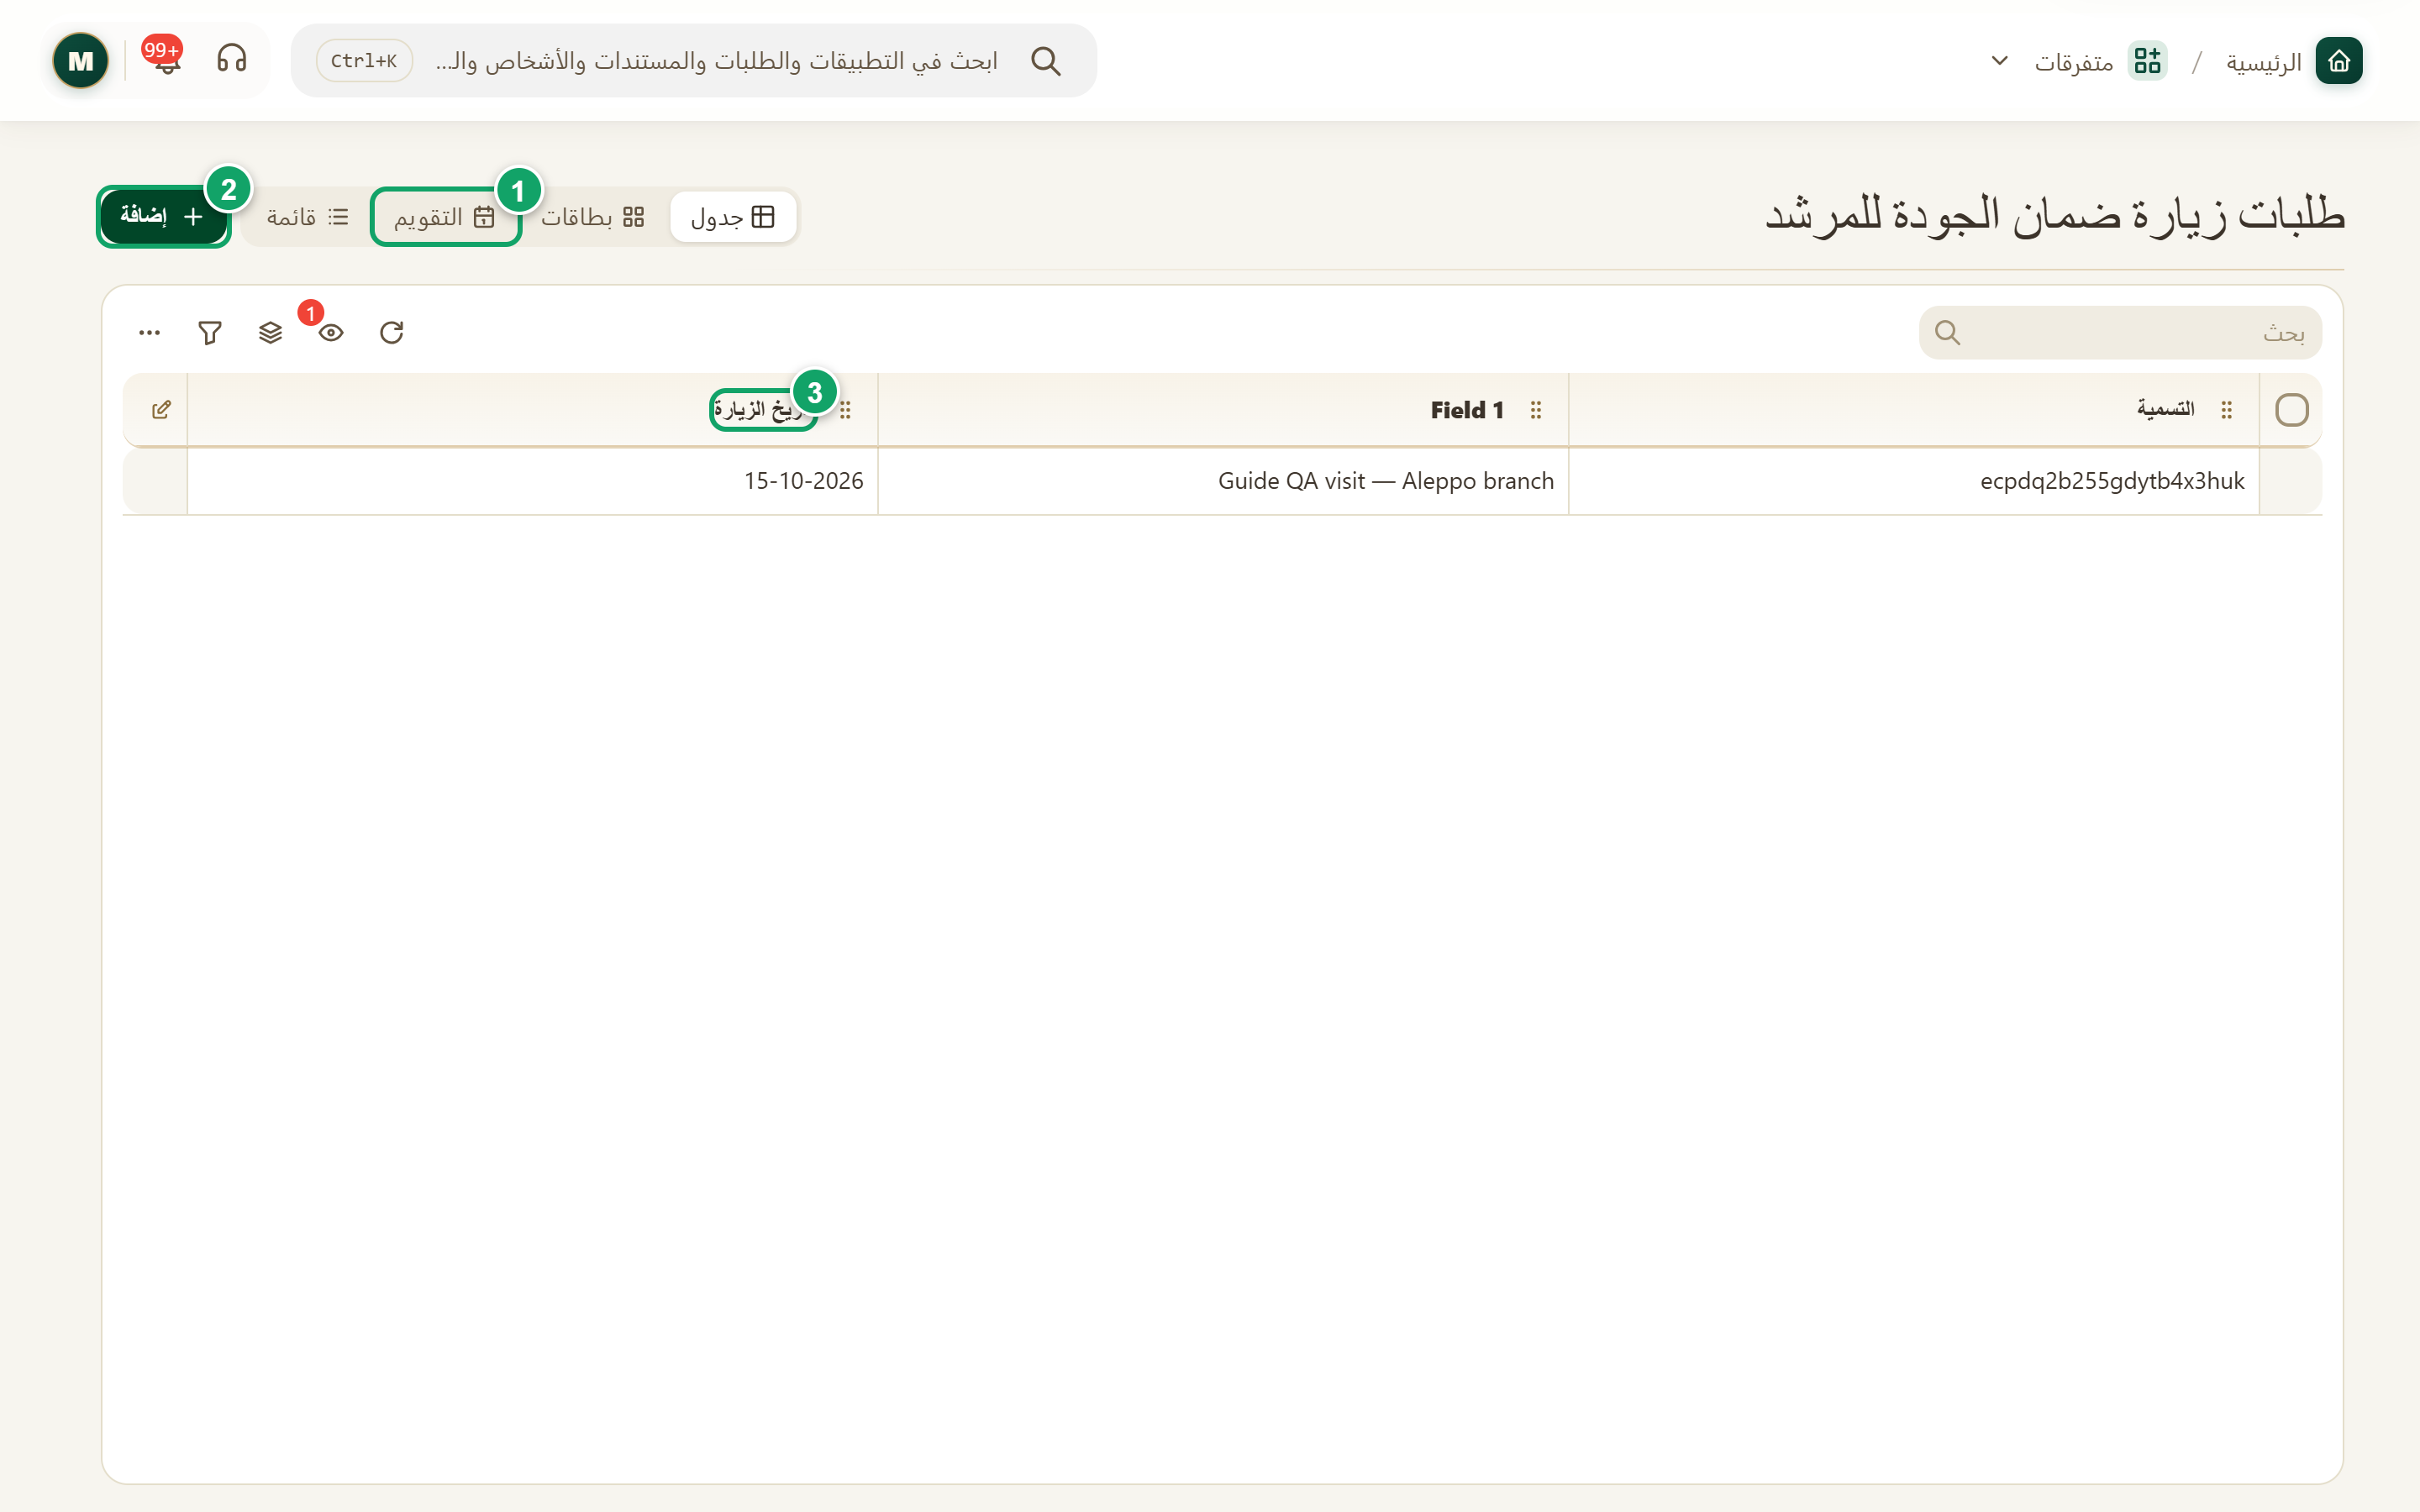
\includegraphics[width=0.95\linewidth,height=0.72\textheight,keepaspectratio]{figures/screens/ch06-records-ar.png}
\caption{قائمة سجلات النوع بعد النشر}
\label{fig:builder-lists-records}
\shotnote{هذه هي القائمة التي يراها المستخدمون بعد النشر، وفيها سجل اختبار أُنشئ في test2 ثم أُعيد فتحه للتحقق من الحفظ. ① «التقويم»: ظهرت طريقة العرض هذه لأن للنوع حقل تاريخ. ② «إضافة». ③ عمود «تاريخ الزيارة»: يعرض القيمة المحفوظة للسجل الاختباري بعد إعادة فتحه.}
\end{figure}


\begin{table}[H]
\centering
\caption{طرق العرض المتاحة}
\label{tab:builder-lists-modes}
\begin{tabularx}{\linewidth}{R{3.6cm} Y}
\rcHeaderRow
\thh{طريقة العرض} & \thh{متى تناسب}\\
جدول وقائمة & متاحان دائماً لمراجعة السجلات ومقارنتها صفاً صفاً، مع الترتيب والتصفية.\\
بطاقات ومعرض & «بطاقات» متاحة دائماً، أما «معرض» فيظهر عندما يكون للنوع حقل «ملف» تُعرض منه الصور.\\
كانبان & يوزّع السجلات في أعمدة حسب الحالة أو قيمة اختيار، ويظهر عندما يوجد حقل مناسب لذلك.\\
التقويم والخط الزمني & يظهران عندما يكون للنوع حقل تاريخ أو نطاق زمني، مثل المواعيد والمراحل.\\
خريطة & تظهر عندما يكون للنوع حقل «موقع» أو «حدود».\\
شجرة & تظهر عندما تفعّل «السجلات الأم» في «إعدادات متقدمة»، فتُعرض السجلات في تسلسل أب وأبناء.\\
\end{tabularx}
\end{table}

\begin{figure}[H]
\centering
\begin{tikzpicture}[node distance=0.5cm]
\node[entity] (fields) {\RL{الحقول}};
\node[entityOpt,below right=0.7cm and 0.3cm of fields] (cal) {\RL{التقويم}};
\node[entityOpt,below left=0.7cm and 0.3cm of fields] (map) {\RL{خريطة}};
\draw[dependsOnOpt] (fields.south) -- ++(0,-0.3) -| (cal.north);
\draw[dependsOnOpt] (fields.south) -- ++(0,-0.3) -| (map.north);
\end{tikzpicture}
\rclegend
\caption{طرق عرض تعتمد على نوع الحقل}
\label{fig:builder-lists-depends}
\shotnote{يوضّح الشكل أن بعض طرق العرض تحتاج إلى حقل من نوع معيّن: فالتقويم يحتاج إلى تاريخ، والخريطة تحتاج إلى موقع أو حدود. لذلك إذا لم تجد طريقة عرض تريدها، فراجع الحقول أولاً، لأن الطريقة لا تظهر في الخيارات دون الحقل الذي تعتمد عليه.}
\end{figure}

\subsection{خطوات العمل والتحقق}
\begin{enumerate}
\item افتح نوع السجلات واختر «القوائم وطرق العرض».
\item فعّل طرق العرض التي يحتاجها الفريق، واختر الطريقة الافتراضية التي تظهر أولاً.
\item اختر الأعمدة الظاهرة ورتّبها حسب أهميتها للعمل اليومي، وأضف الأرقام الملخّصة عند الحاجة.
\end{enumerate}

\textbf{تحقق ومعالجة المشكلة:} يجب أن تعرض «نظرة عامة» الطريقة الافتراضية وعدد العروض المحفوظة. وبعد النشر افتح قائمة السجلات وبدّل بين الطرق للتأكد منها؛ فإذا كانت طريقة العرض فارغة، فتحقق من أن السجلات تحمل قيمة في الحقل الذي تعتمد عليه.

\clearpage
\section{المؤشرات والعروض المحفوظة}
\label{sec:builder-feature-figures-views}

تساعد هاتان الأداتان الفريق على فهم القائمة دون أن يفتح كل سجل. فـ«المؤشرات» أرقام تلخيصية تظهر فوق القائمة، مثل عدد الطلبات المفتوحة أو مجموع المبالغ، والضغط على أي مؤشر يصفّي القائمة. أما «العروض المحفوظة» فتبويبات فوق القائمة، لكل منها تصفية وترتيب وتجميع جاهز، فينتقل المستخدم بين «طلباتي» و«بانتظار المراجعة» بضغطة واحدة.

\textbf{المسار ومن يستخدمه:} «المنشئ» ← «القوائم وطرق العرض» ← بطاقة «المؤشرات» وبطاقة «العروض المحفوظة». يضبطها من يبني النوع، ويراها كل من يفتح القائمة. ويستطيع كل مستخدم أن يحفظ عروضاً خاصة به من القائمة نفسها.

\begin{rcnote}[مثال: شركة الأفق]
يضيف المسؤول فوق قائمة «طلبات الزيارة» مؤشراً بعدد الطلبات «قيد المراجعة» يظهر بلون التحذير إذا زاد على خمسة، وعرضاً محفوظاً باسم «بانتظار مراجعتي» يعرض لسارة الخطيب الطلبات التي تنتظرها.
\end{rcnote}

\begin{figure}[H]
\centering
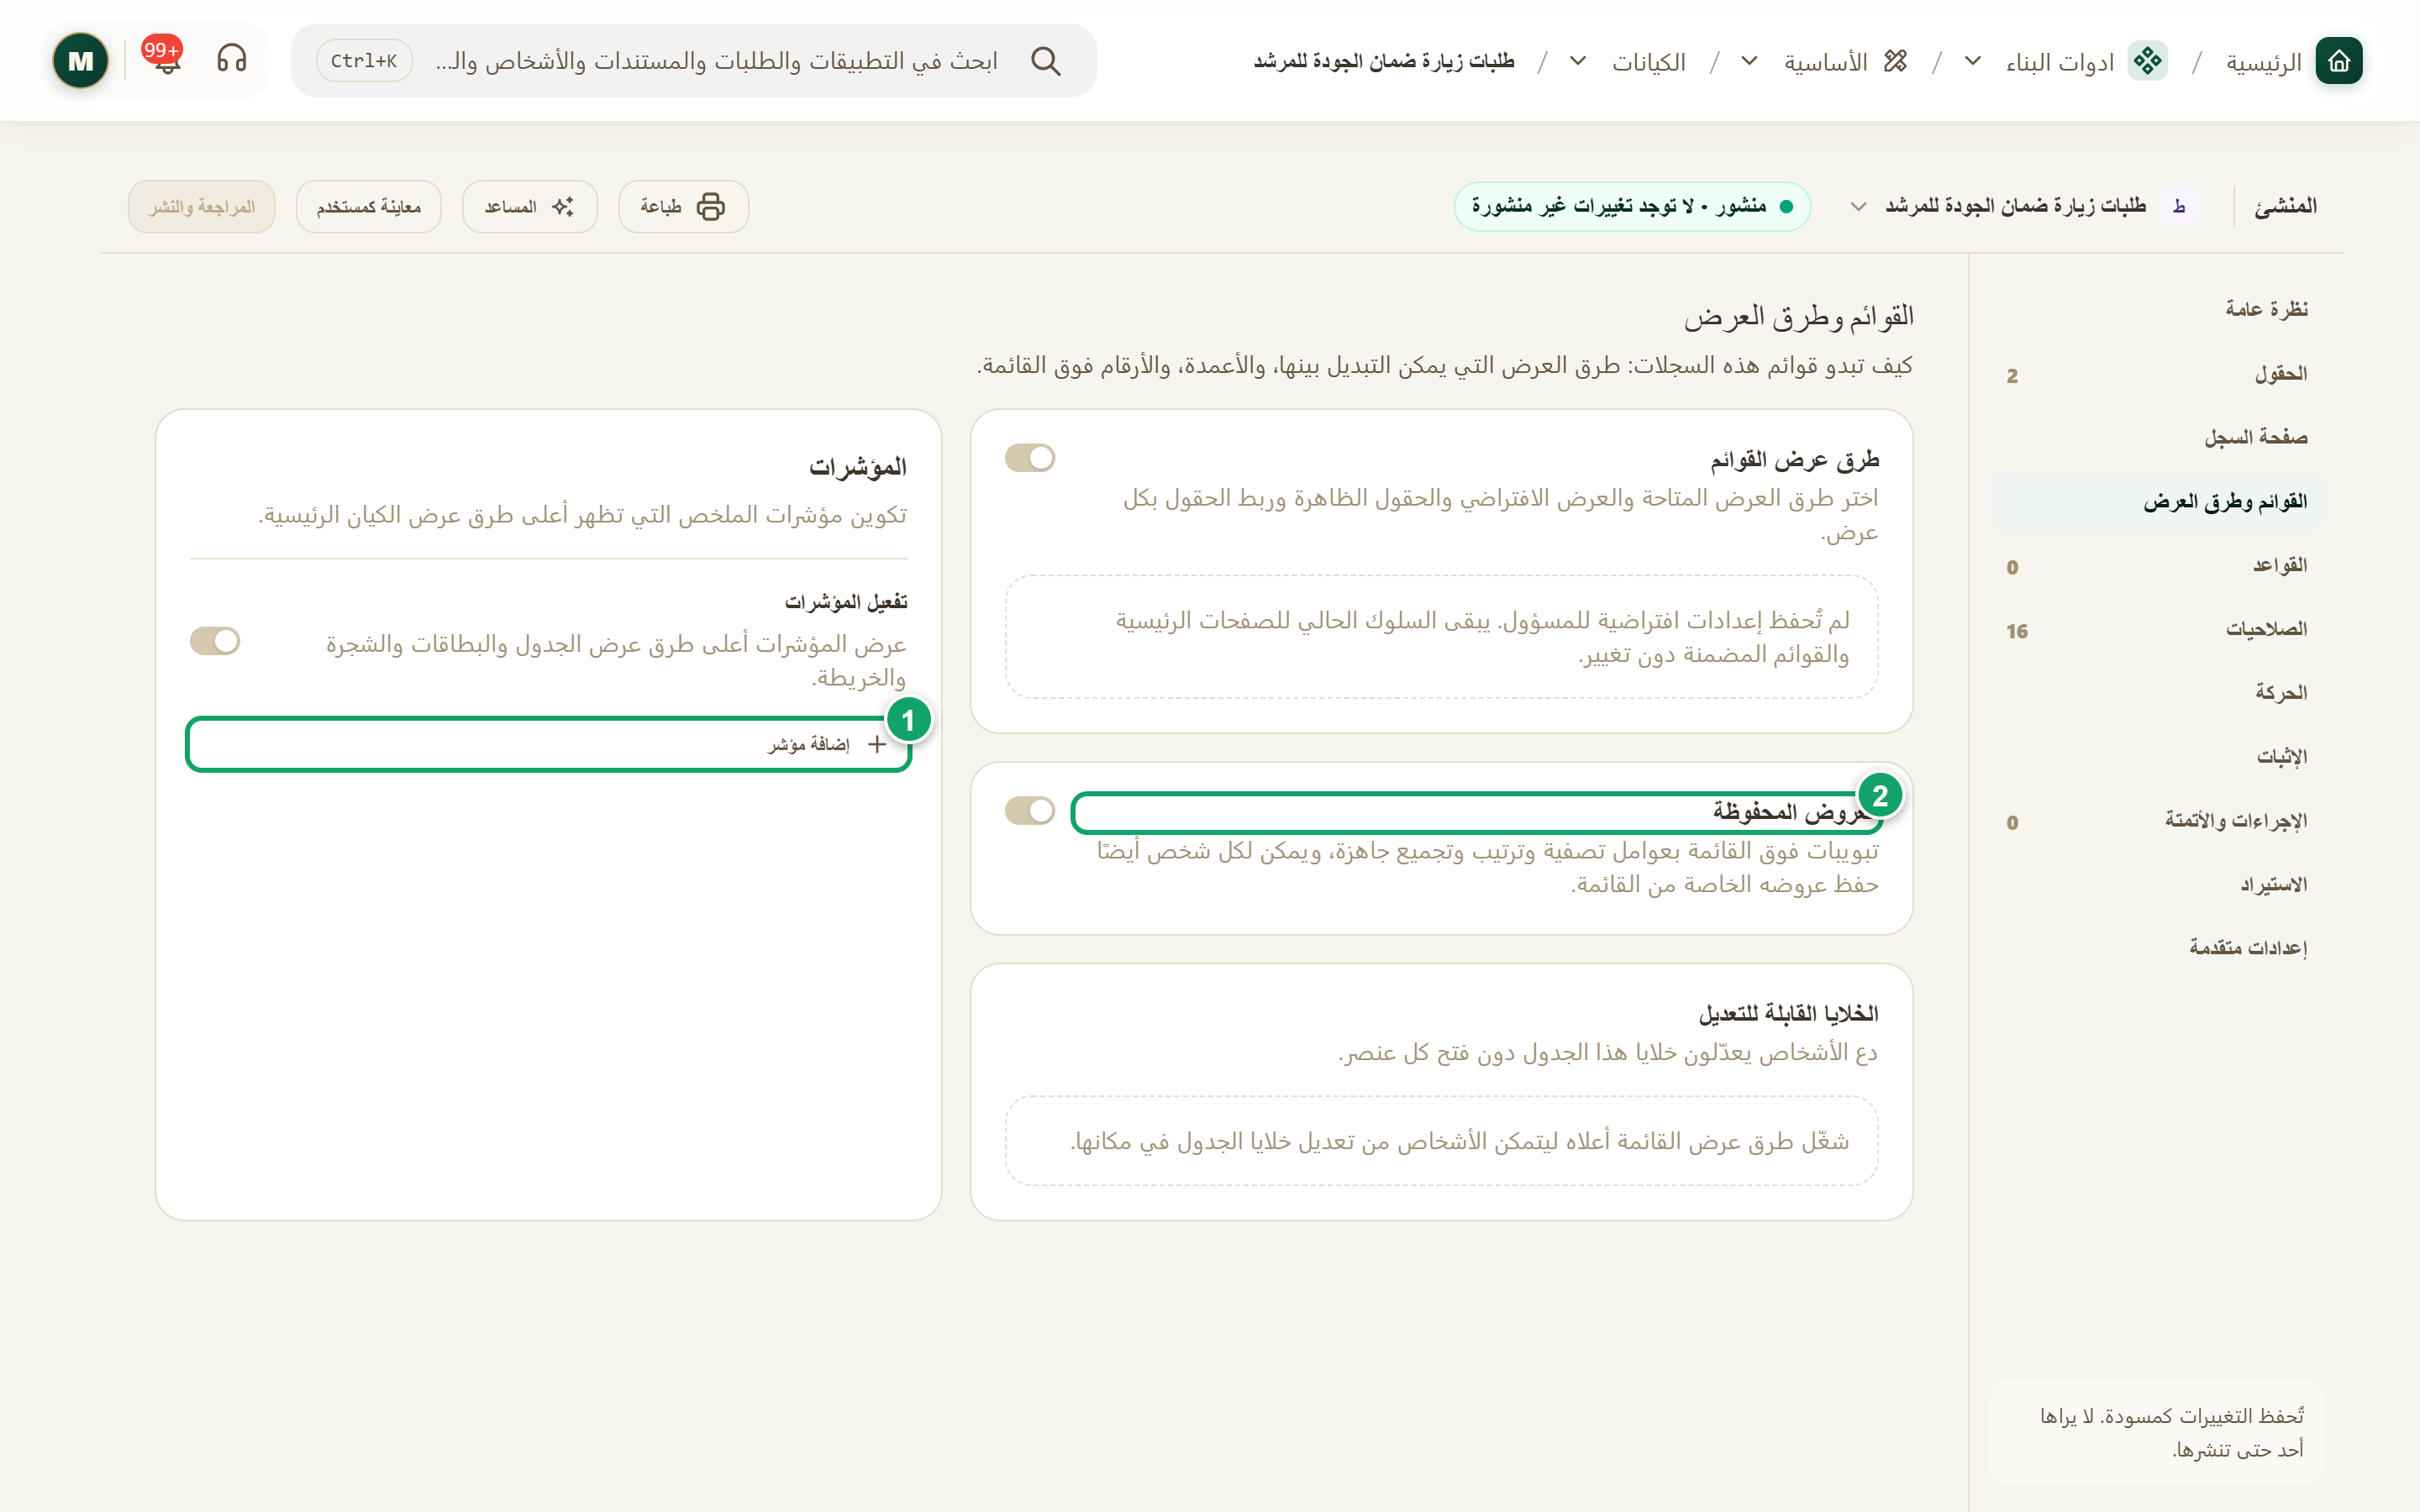
\includegraphics[width=0.95\linewidth,height=0.72\textheight,keepaspectratio]{figures/screens/ch06-ws-figures-views-ar.png}
\caption{بطاقتا المؤشرات والعروض المحفوظة في «القوائم وطرق العرض»}
\label{fig:builder-figures-views-screen}
\shotnote{تعرض الصورة قسم «القوائم وطرق العرض» في النوع الاختباري، ولم يُضف إليه بعد أي مؤشر أو عرض محفوظ. ويبيّن ذلك أين تبدأ عندما تريد تلخيص القائمة أو تنظيمها. ① «إضافة مؤشر»: يضيف رقماً تلخيصياً فوق القائمة. ② «العروض المحفوظة»: البطاقة التي تضيف منها تبويبات جاهزة فوق القائمة.}
\end{figure}

\begin{table}[H]
\centering
\caption{إعدادات المؤشر}
\label{tab:builder-figures-settings}
\begin{tabularx}{\linewidth}{R{3.6cm} Y}
\rcHeaderRow
\thh{الإعداد} & \thh{المعنى}\\
نوع المؤشر & «قيمة واحدة»، أو «نسبة (جزء من إجمالي)» تُعرض مع شريط، أو «التوزيع حسب الحالة».\\
الحساب & العدد، أو المجموع، أو المتوسط، أو الأدنى، أو الأعلى، أو المتوسط المرجّح لحقل رقمي.\\
السجلات المحسوبة & سجلات هذا النوع أو نوع مرتبط به، مع فلاتر ونطاق تاريخ، مثل آخر ثلاثين يوماً.\\
سطر تحت المؤشر & لا شيء، أو نص، أو قيمة ثانية، أو أقرب سجل قادم.\\
التمييز & يلوّن المؤشر بلون «تحذير» أو «حرج» عندما تقل القيمة عن حد أو تزيد عليه.\\
\end{tabularx}
\end{table}

\begin{table}[H]
\centering
\caption{ما يحفظه العرض المحفوظ}
\label{tab:builder-saved-views-settings}
\begin{tabularx}{\linewidth}{R{3.6cm} Y}
\rcHeaderRow
\thh{الإعداد} & \thh{المعنى}\\
الاسم واللون & اسم التبويب ولونه فوق القائمة، ويمكن أن يظهر عليه عدد السجلات.\\
يفتح في & طريقة العرض التي يفتح بها التبويب، أو الإبقاء على طريقة العرض الحالية.\\
الترتيب والتجميع & الحقل الذي تُرتب به السجلات واتجاه الترتيب، والحقل الذي تُجمع حسبه.\\
الفلاتر & الشروط التي تحدد السجلات الظاهرة، ويمكن أن تتبع المستخدم نفسه، مثل «أنا» أو عدد أيام من اليوم.\\
السجلات التي يستطيع المستخدم العمل عليها & يعرض فقط السجلات التي يستطيع المستخدم تنفيذ انتقال عليها في حقل الحالة.\\
\end{tabularx}
\end{table}

\begin{figure}[H]
\centering
\begin{tikzpicture}[node distance=0.5cm]
\node[stepBox] (a) {\RL{تفعيل المؤشرات}};
\node[stepBox,below=of a] (b) {\RL{إضافة مؤشر وضبطه}};
\node[stepBox,below=of b] (c) {\RL{إضافة عرض محفوظ}};
\node[stepBox,below=of c] (d) {\RL{المراجعة والنشر}};
\node[stepBox,below=of d] (e) {\RL{التجربة في القائمة}};
\draw[flowsTo] (a) -- (b);
\draw[flowsTo] (b) -- (c);
\draw[flowsTo] (c) -- (d);
\draw[flowsTo] (d) -- (e);
\end{tikzpicture}
\rclegend
\caption{تلخيص القائمة وتنظيمها}
\label{fig:builder-figures-views-flow}
\shotnote{يجمع المخطط الأداتين في مسار واحد لأنهما تعملان فوق القائمة نفسها: المؤشر يلخّص والعرض المحفوظ يصفّي. وينتهي بالتجربة في القائمة بعد النشر، لأن الضغط على المؤشر والتنقل بين التبويبات لا يظهران إلا هناك.}
\end{figure}

\subsection{خطوات العمل والتحقق}
\begin{enumerate}
\item افتح «القوائم وطرق العرض»، وفعّل «تفعيل المؤشرات»، ثم اضغط «إضافة مؤشر».
\item اختر نوع المؤشر والحساب والحقل، وأضف الفلاتر ونطاق التاريخ، ثم حدد التمييز إن احتجت إلى تنبيه بصري.
\item في «العروض المحفوظة» فعّل إظهار التبويبات، واضغط «إضافة عرض»، واكتب اسمه وفلاتره وترتيبه.
\item انشر التغييرات، ثم افتح القائمة واضغط المؤشر والتبويب الجديد.
\end{enumerate}

\textbf{تحقق ومعالجة المشكلة:} يجب أن يظهر المؤشر فوق القائمة، وأن يصفّيها عند الضغط عليه، وأن يعرض التبويب السجلات المطابقة لفلاتره. فإذا لم يظهر المؤشر، فتأكد أن «تفعيل المؤشرات» مفعّل وأن المؤشر غير مخفي. وتذكّر أن العروض التي تضيفها هنا يراها الجميع، أما «حفظ العرض» في القائمة فيحفظ عرضاً لا يراه غيرك.

\clearpage
\section{القواعد}
\label{sec:builder-feature-rules}

القاعدة تجعل السجل يتصرف بحسب ما فيه من قيم، دون أن يتذكر المستخدم ذلك بنفسه. فقد تُظهر حقلاً عند اختيار قيمة معينة، أو تقفله بعد الإنشاء، أو تجعله إلزامياً في حالة محددة، أو ترفض قيمة غير منطقية. ويجمع قسم «القواعد» هذه القواعد كلها في قائمة واحدة.

\textbf{المسار ومن يستخدمه:} نوع السجلات ← «القواعد». يستخدمه من يبني النوع، بعد أن تكتمل الحقول.

\begin{rcnote}[مثال: شركة الأفق]
يضيف مسؤول النظام قاعدة تُظهر حقل «سبب الرفض» عندما تكون الحالة «مرفوض» فقط، وقاعدة تتحقق من أن موعد الزيارة يقع في تاريخ الطلب أو بعده. ويضيف القاعدتين من ①.
\end{rcnote}

\begin{figure}[H]
\centering
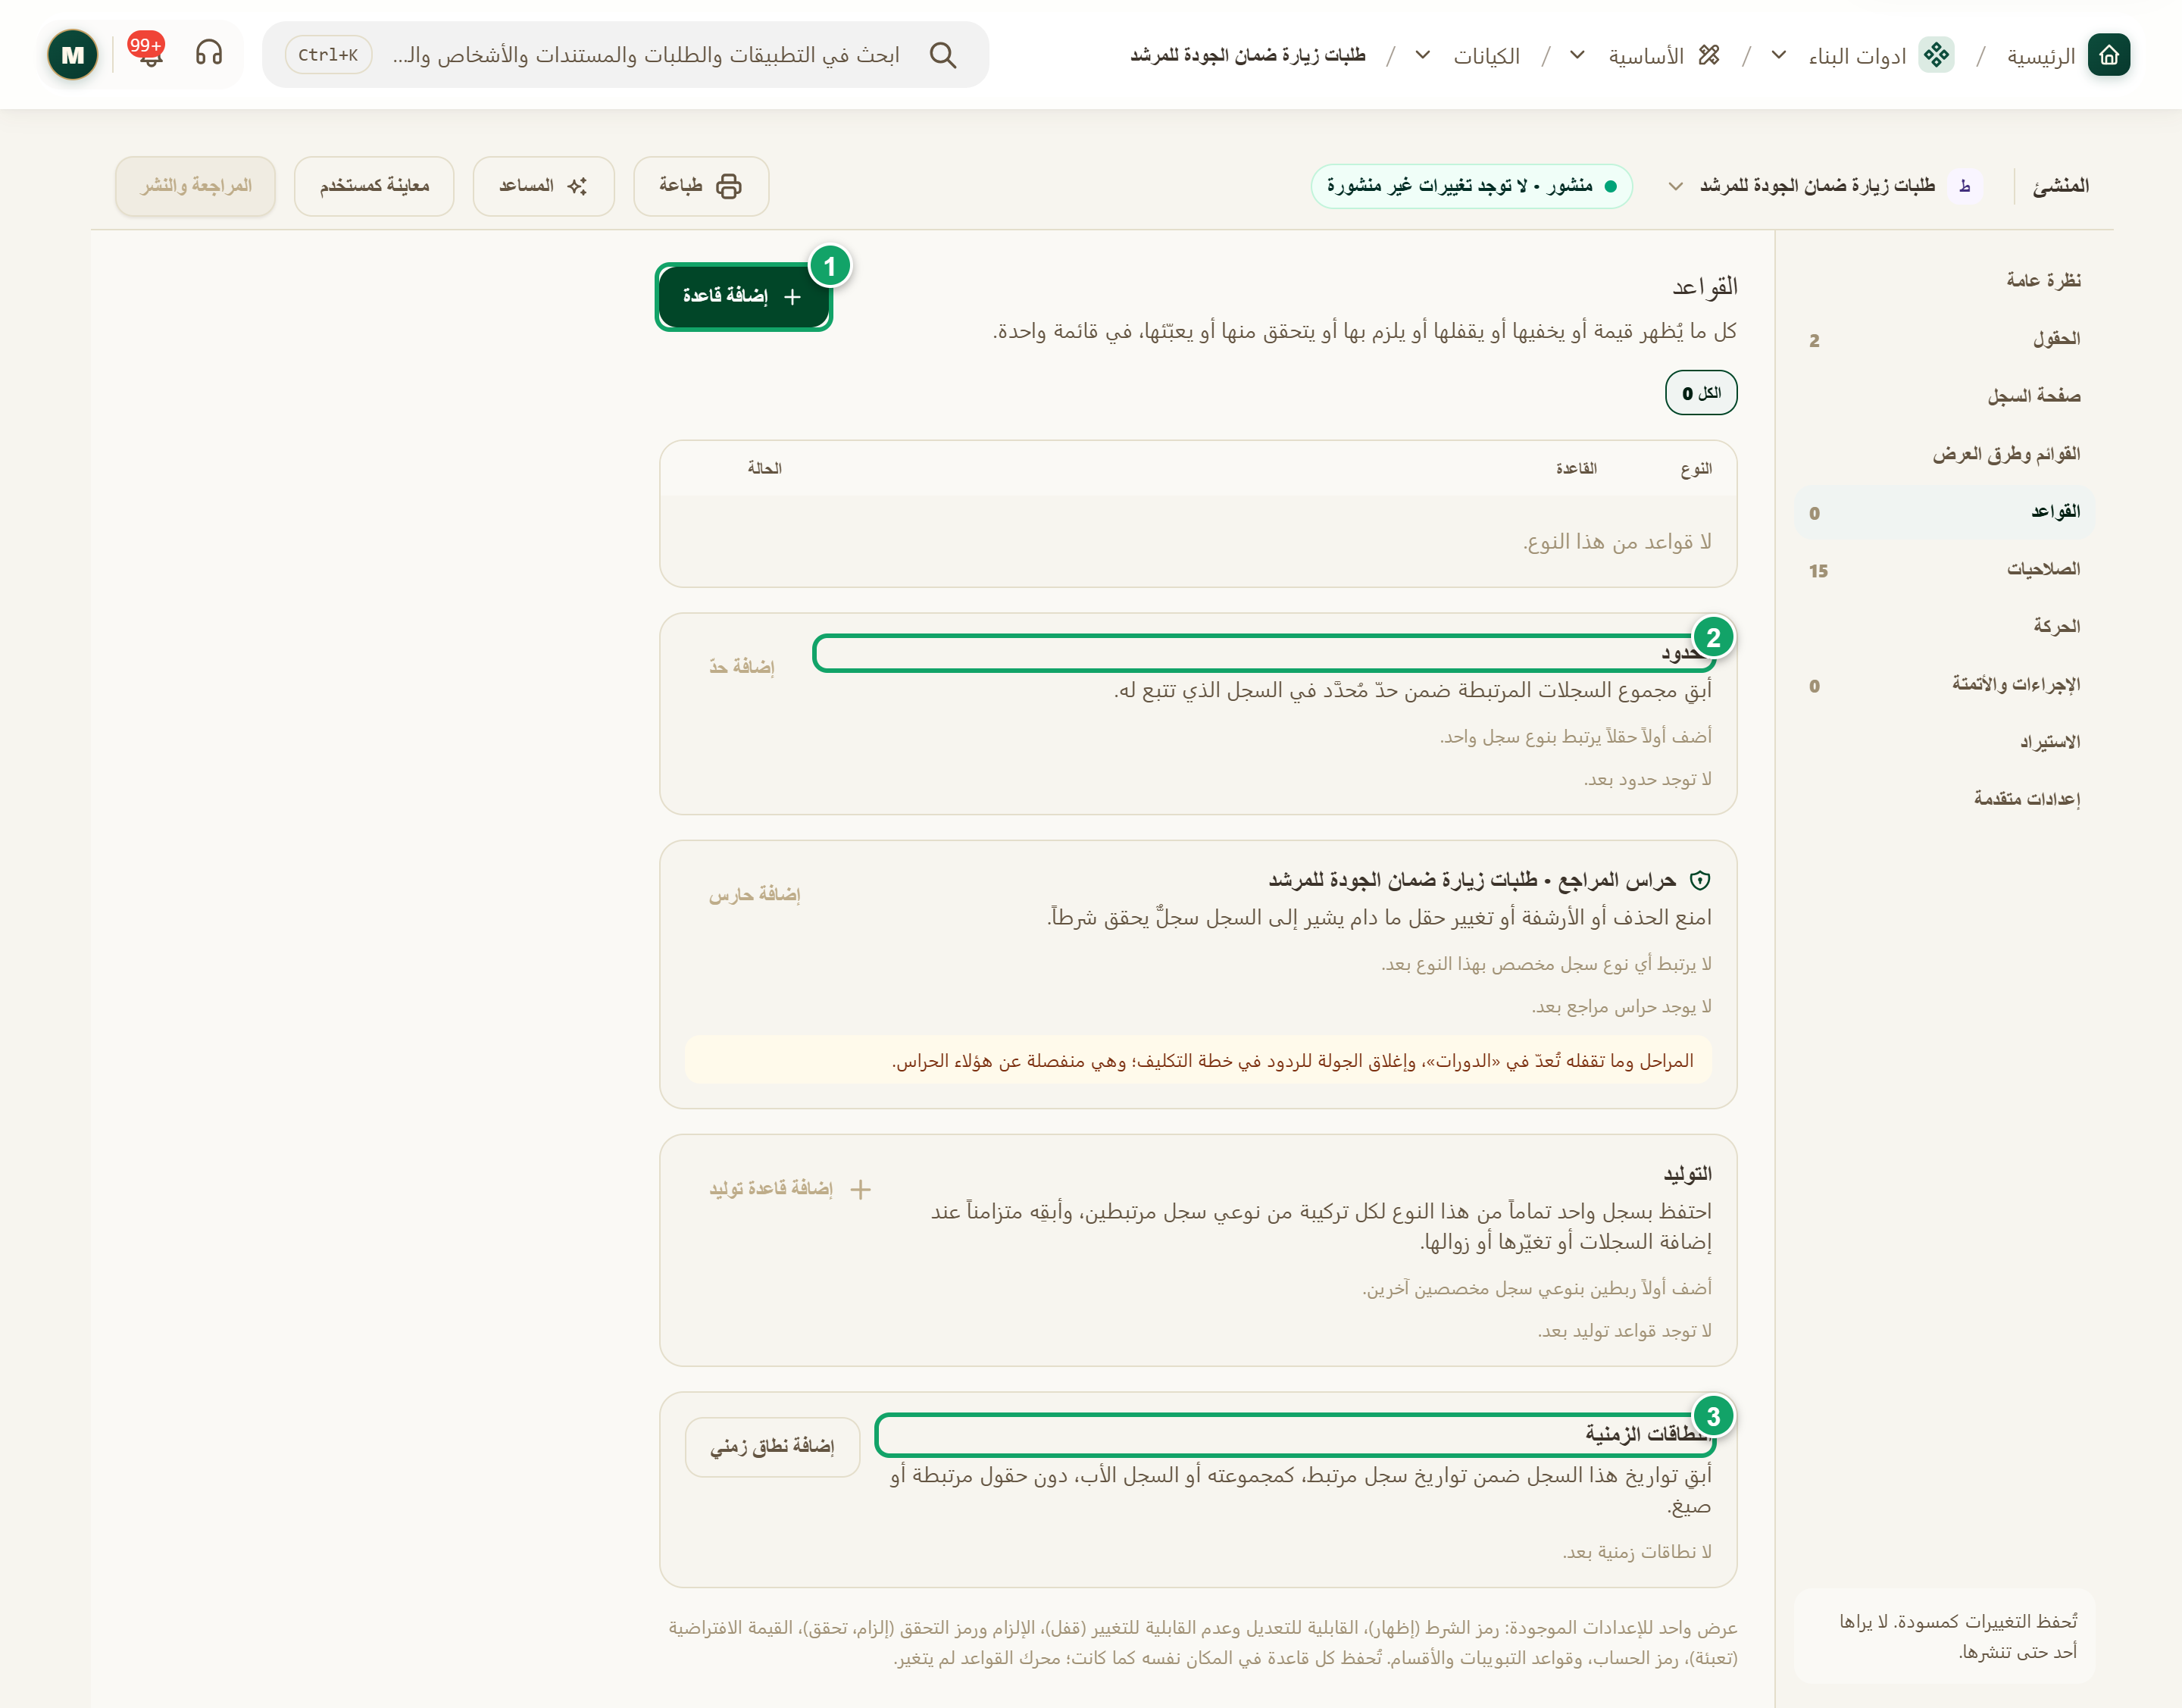
\includegraphics[width=0.95\linewidth,height=0.72\textheight,keepaspectratio]{figures/screens/ch06-ws-rules-ar.png}
\caption{قسم «القواعد» وأدواته الإضافية}
\label{fig:builder-rules-screen}
\shotnote{تظهر في أعلى القسم قائمة القواعد، وتحتها أدوات أخرى تحمي البيانات، مثل الحدود والنطاقات الزمنية. والقائمة فارغة لأن النوع الاختباري بلا قواعد. ① «إضافة قاعدة». ② «الحدود»: تُبقي مجموع السجلات المرتبطة ضمن حدّ. ③ «النطاقات الزمنية»: تُبقي تواريخ السجل ضمن تواريخ سجل مرتبط.}
\end{figure}


\begin{table}[H]
\centering
\caption{أنواع القواعد}
\label{tab:builder-rules-kinds}
\begin{tabularx}{\linewidth}{R{3.6cm} Y}
\rcHeaderRow
\thh{النوع} & \thh{ماذا تفعل؟}\\
إظهار أو إخفاء & تُظهر حقلاً أو تبويباً أو قسماً عندما يتحقق شرط، وتخفيه في غير ذلك.\\
قفل التعديل & تمنع تغيير حقل أو تبويب أو قسم: «مقفل عندما» يتحقق شرط، أو «قابل للتعديل فقط عندما»، أو «بعد الإنشاء».\\
إلزام & تجعل الحقل إلزامياً «دائمًا» أو «فقط عندما» يتحقق شرط، مع رسالة توضح السبب.\\
تحقق من القيمة & ترفض القيمة إن لم تكن، مثلاً، أكبر من رقم أو بعد تاريخ أو مختلفة عن حقل آخر، وتعرض رسالتك.\\
تعبئة قيمة & تبدأ الحقل بقيمة جاهزة يستطيع المستخدم تغييرها.\\
حساب & تعرض الحقول المحسوبة؛ وتعديلها يتم من قسم «الحقول».\\
\end{tabularx}
\end{table}

\begin{table}[H]
\centering
\caption{قواعد أخرى ليست في هذا القسم}
\label{tab:builder-rules-other}
\begin{tabularx}{\linewidth}{R{3.6cm} Y}
\rcHeaderRow
\thh{القاعدة} & \thh{أين تجدها؟}\\
الحدود & أسفل قائمة القواعد: تُبقي مجموع السجلات المرتبطة أو عددها ضمن حدّ، ثم ترفض التجاوز أو تنبّه وتطلب تبريراً.\\
قواعد دورة الحياة & في حقل «الحالة» داخل «الحقول»: لكل حالة تحدد إن كان السجل «مقفل» أو «مقفل باستثناء…»، ويمكنك «منع الحذف». تحتاج إلى قالب حالات ثابت.\\
القيم الفريدة & في «إعدادات متقدمة»: تمنع تكرار رمز أو مجموعة قيم بين سجلين.\\
\end{tabularx}
\end{table}

\begin{figure}[H]
\centering
\begin{tikzpicture}[node distance=0.5cm]
\node[stepBox] (a) {\RL{اختيار نوع القاعدة}};
\node[stepBox,below=of a] (b) {\RL{الشرط: عندما…}};
\node[stepBox,below=of b] (c) {\RL{الهدف: حقل أو تبويب أو قسم}};
\node[stepBox,below=of c] (d) {\RL{جرّبها ثم احفظ في المسودة}};
\draw[flowsTo] (a) -- (b);
\draw[flowsTo] (b) -- (c);
\draw[flowsTo] (c) -- (d);
\end{tikzpicture}
\rclegend
\caption{كيف تُبنى القاعدة}
\label{fig:builder-rules-flow}
\shotnote{تُقرأ القاعدة كجملة: «عندما» يتحقق شرط، نفّذ أثراً على هدف محدد. ويضع المخطط التجربة قبل الحفظ، لأن «جرّبها» يطبّق القاعدة على سجلات عينة فيكشف الشرط الخاطئ قبل أن يصل إلى المستخدمين. وتنطبق القواعد على كل من يستطيع تعديل السجل، فلا تُستخدم لتمييز دور من آخر.}
\end{figure}

\subsection{خطوات العمل والتحقق}
\begin{enumerate}
\item افتح نوع السجلات واختر «القواعد»، ثم اضغط «إضافة قاعدة».
\item اختر نوع القاعدة، ثم ابنِ الشرط تحت «عندما» واربط الشروط بـ«+ و» أو «+ أو».
\item اختر الهدف من «اختر حقلًا أو تبويبًا أو قسمًا»، واكتب «الرسالة التي تظهر للناس» عند الحاجة.
\item اضغط «جرّبها» وراجع النتيجة على العينات، ثم اضغط «حفظ في المسودة».
\end{enumerate}

\textbf{تحقق ومعالجة المشكلة:} يجب أن تظهر القاعدة في الجدول بحالة «سليمة». فإذا ظهرت «معطّلة»، فافتحها وصحّح الحقل أو الشرط الذي تغيّر. وإذا أردت أن يرى بعض الأدوار حقلاً دون غيرهم، فاستخدم «الصلاحيات» لا «القواعد».

\clearpage
\section{الحدود وحراس المراجع والتوليد والنطاقات الزمنية}
\label{sec:builder-feature-record-limits}

تقع هذه الأدوات الأربع أسفل جدول القواعد في قسم «القواعد»، وتحمي البيانات من أخطاء يصعب اكتشافها لاحقاً. فـ«الحدود» تمنع أن يتجاوز مجموع السجلات المرتبطة حداً معيناً، و«حراس المراجع» تمنع حذف سجل أو تغييره ما دامت سجلات أخرى تعتمد عليه، و«التوليد» يُبقي سجلاً واحداً لكل تركيبة من نوعين مرتبطين، و«النطاقات الزمنية» تُبقي تواريخ السجل داخل تواريخ سجل مرتبط.

\textbf{المسار ومن يستخدمه:} «المنشئ» ← «القواعد»، ثم أسفل الصفحة: «الحدود» و«حراس المراجع» و«التوليد» و«النطاقات الزمنية». يستخدمها من يبني الأنواع المالية والتنظيمية التي تحتاج إلى ضوابط بين السجلات.

\begin{rcnote}[مثال: شركة الأفق]
يضيف المسؤول نطاقاً زمنياً يُبقي تاريخ الزيارة داخل تواريخ خطة الزيارات المرتبطة بالطلب، وحارساً يمنع حذف فرع ما دامت له طلبات زيارة مفتوحة.
\end{rcnote}

\begin{figure}[H]
\centering
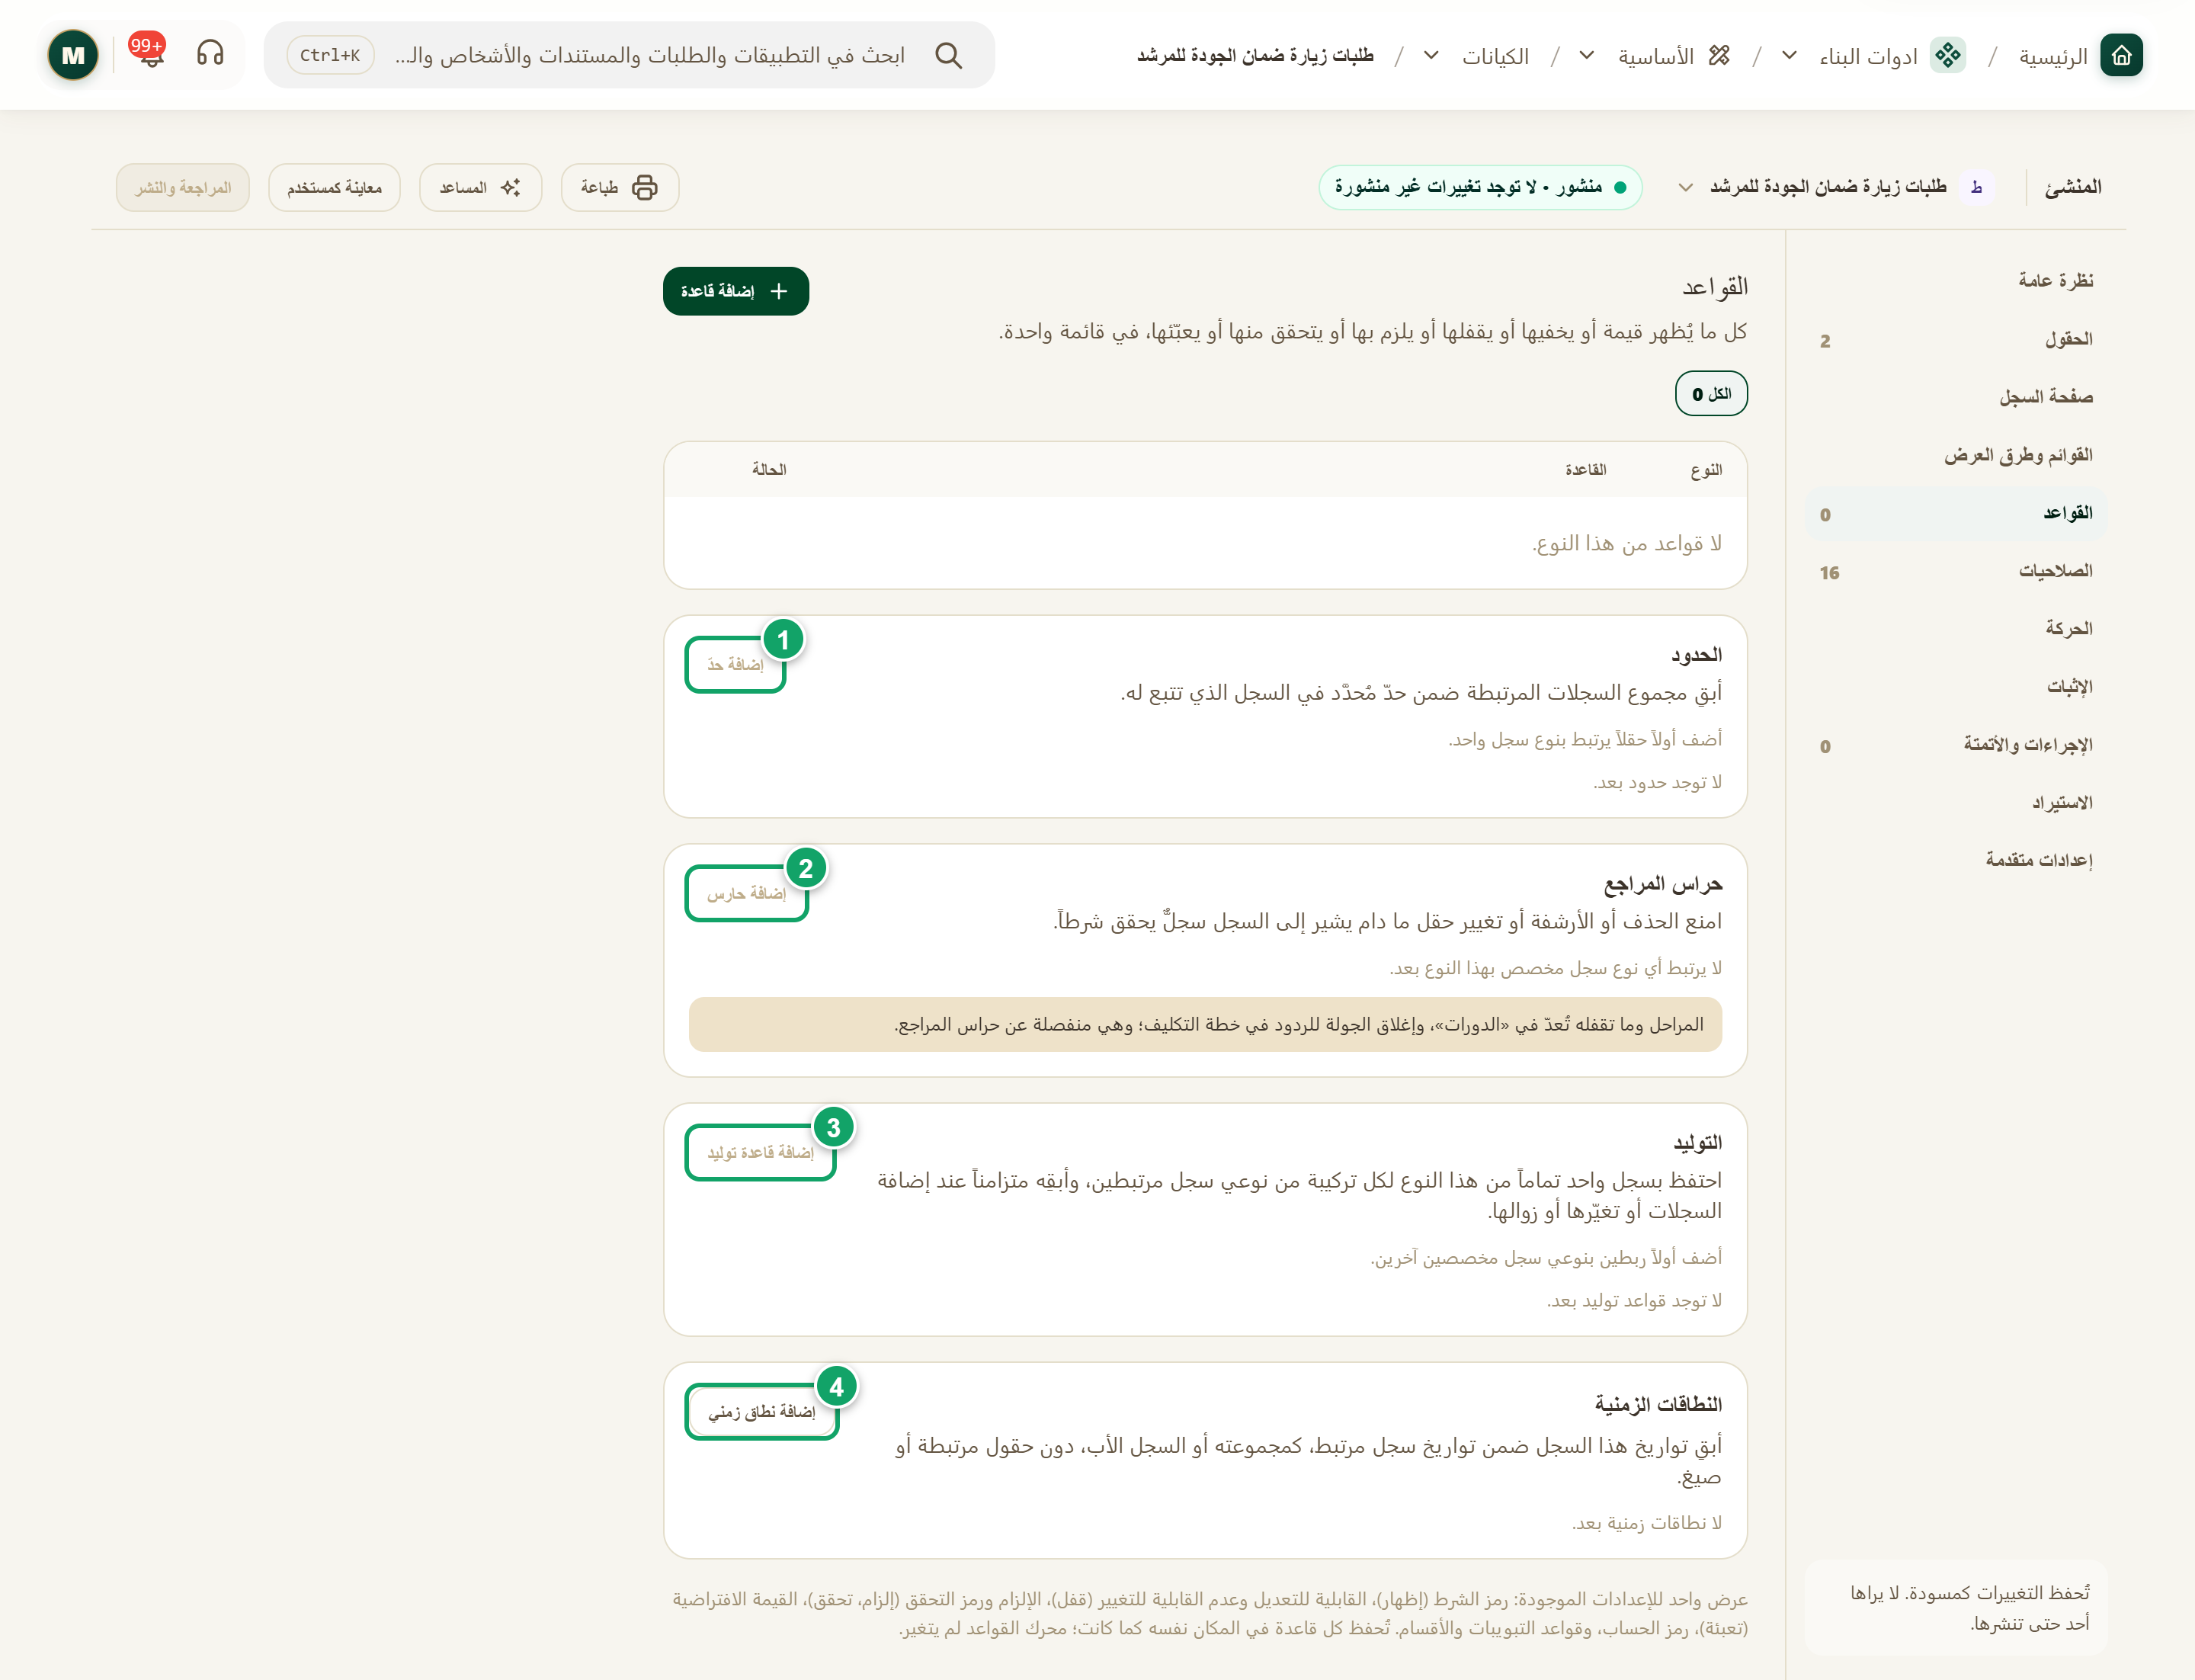
\includegraphics[width=0.95\linewidth,height=0.72\textheight,keepaspectratio]{figures/screens/ch06-ws-rule-tools-ar.png}
\caption{الأدوات الأربع أسفل جدول القواعد}
\label{fig:builder-record-limits-screen}
\shotnote{تعرض الصورة قسم «القواعد» في النوع الاختباري، وتحت جدول القواعد بطاقة لكل أداة مع زر الإضافة الخاص بها. وتظهر في كل بطاقة رسالة تبيّن ما يلزم قبل استخدامها، مثل حقل علاقة. ① «إضافة حدّ». ② «إضافة حارس». ③ «إضافة قاعدة توليد». ④ «إضافة نطاق زمني». ويبدأ كل زر محرراً يقودك إلى إكمال الجملة التي تصف الضابط.}
\end{figure}

\begin{table}[H]
\centering
\caption{الأدوات الأربع}
\label{tab:builder-record-limits-tools}
\begin{tabularx}{\linewidth}{R{3.6cm} Y}
\rcHeaderRow
\thh{الأداة} & \thh{ما تفعله وما تضبطه}\\
الحدود & تُبقي مجموع السجلات المرتبطة ضمن حد يحدده السجل الذي تتبع له، مثل مجموع بنود الصرف ضمن الموازنة. تضبط فيها «ما يُجمع» و«النطاق» و«الحدّ»، وما يحدث «عند التجاوز»: الرفض، أو التحذير مع طلب سبب يصل إلى أدوار تقرر فيه.\\
حراس المراجع & ترفض حذف السجل أو أرشفته أو تغيير حقل فيه ما دامت سجلات أخرى تشير إليه وتطابق شرطاً، مع رسالة توضح السبب. ويمكن إضافة عشرة حراس على الأكثر لكل نوع.\\
التوليد & يُبقي سجلاً واحداً من هذا النوع لكل تركيبة من سجلات نوعين مرتبطين، ويحدّثه عند تغيّرهما، مثل سجل تقييم لكل موظف في كل دورة. وتعرض «المعاينة» عدد السجلات، و«تعبئة الآن» تنشئ الناقص منها، ولا يعمل قبل نشر النوع.\\
النطاقات الزمنية & تُبقي تاريخي البداية والنهاية داخل تواريخ سجل مرتبط أو السجل الأم، وتحدد ما يحدث عند تغيّر تواريخه: السماح مع إظهار السجلات الخارجة، أو رفض التغيير. ويرى المستخدم في السجل عبارة مثل «بين … و…».\\
\end{tabularx}
\end{table}

\begin{figure}[H]
\centering
\begin{tikzpicture}[node distance=0.5cm]
\node[stepBox] (a) {\RL{تحديد الخطر على البيانات}};
\node[stepBox,below=of a] (b) {\RL{اختيار الأداة المناسبة}};
\node[stepBox,below=of b] (c) {\RL{ضبطها وكتابة رسالتها}};
\node[stepBox,below=of c] (d) {\RL{المعاينة أو التجربة}};
\node[stepBox,below=of d] (e) {\RL{المراجعة والنشر}};
\draw[flowsTo] (a) -- (b);
\draw[flowsTo] (b) -- (c);
\draw[flowsTo] (c) -- (d);
\draw[flowsTo] (d) -- (e);
\end{tikzpicture}
\rclegend
\caption{إضافة ضابط بين السجلات}
\label{fig:builder-record-limits-flow}
\shotnote{يبدأ المخطط بتحديد الخطر لا بالأداة، لأن كل أداة تعالج خطراً مختلفاً: تجاوز مبلغ، أو حذف سجل مستخدم، أو سجلات ناقصة، أو تواريخ متعارضة. وتأتي كتابة الرسالة مع الضبط لأن المستخدم الذي يُرفض تعديله يحتاج إلى سبب واضح ليعرف ما يفعل.}
\end{figure}

\subsection{خطوات العمل والتحقق}
\begin{enumerate}
\item حدد الخطر الذي تريد منعه، ثم افتح «القواعد» وانزل إلى الأداة المناسبة.
\item اضغط زر الإضافة في الأداة، مثل «إضافة حدّ»، وأكمل الجملة التي يعرضها المحرر خطوة بخطوة.
\item اكتب رسالة تشرح للمستخدم سبب الرفض وما يمكنه فعله.
\item استخدم «المعاينة» إن توفرت، ثم انشر التغييرات وجرّب الحالة الممنوعة بسجل تجريبي.
\end{enumerate}

\textbf{تحقق ومعالجة المشكلة:} يجب أن يُرفض التعديل الممنوع مع رسالتك، وأن يُقبل التعديل السليم. فإذا ظهر في «قبل النشر» أن إعدادات حدّ أو حارس أو توليد غير صالحة، فافتحها من زر الإصلاح وأكمل الحقل الناقص. وتذكّر أن التوليد يحتاج إلى نشر النوع قبل أن يعمل.

\clearpage
\section{الصلاحيات}
\label{sec:builder-feature-access}

تحدد الصلاحيات من يستطيع أن يفعل ماذا في سجلات هذا النوع. وتُسمّى هذه الأعمال «الأفعال»، مثل الرؤية في القوائم والفتح والإضافة والتغيير والحذف. ويعرض قسم «الصلاحيات» الأدوار والأفعال في جدول واحد، وهو يعدّل الأدوار نفسها الموجودة في الإعدادات ← الأدوار، فلا يُنشئ نظاماً ثانياً للصلاحيات.

\textbf{المسار ومن يستخدمه:} نوع السجلات ← «الصلاحيات». يستخدمه من يبني النوع ويملك صلاحية تحديث الأدوار.

\begin{rcnote}[مثال: شركة الأفق]
يمنح مسؤول النظام منسقي الفروع، ومنهم عمر حداد، فعلَي الإضافة والفتح في «طلبات الزيارة»، ويمنح مديرة الموارد البشرية سارة الخطيب فعل التغيير لتسجّل قرارها. ثم يتأكد من صلاحية عمر بالأداة ③.
\end{rcnote}

\begin{figure}[H]
\centering
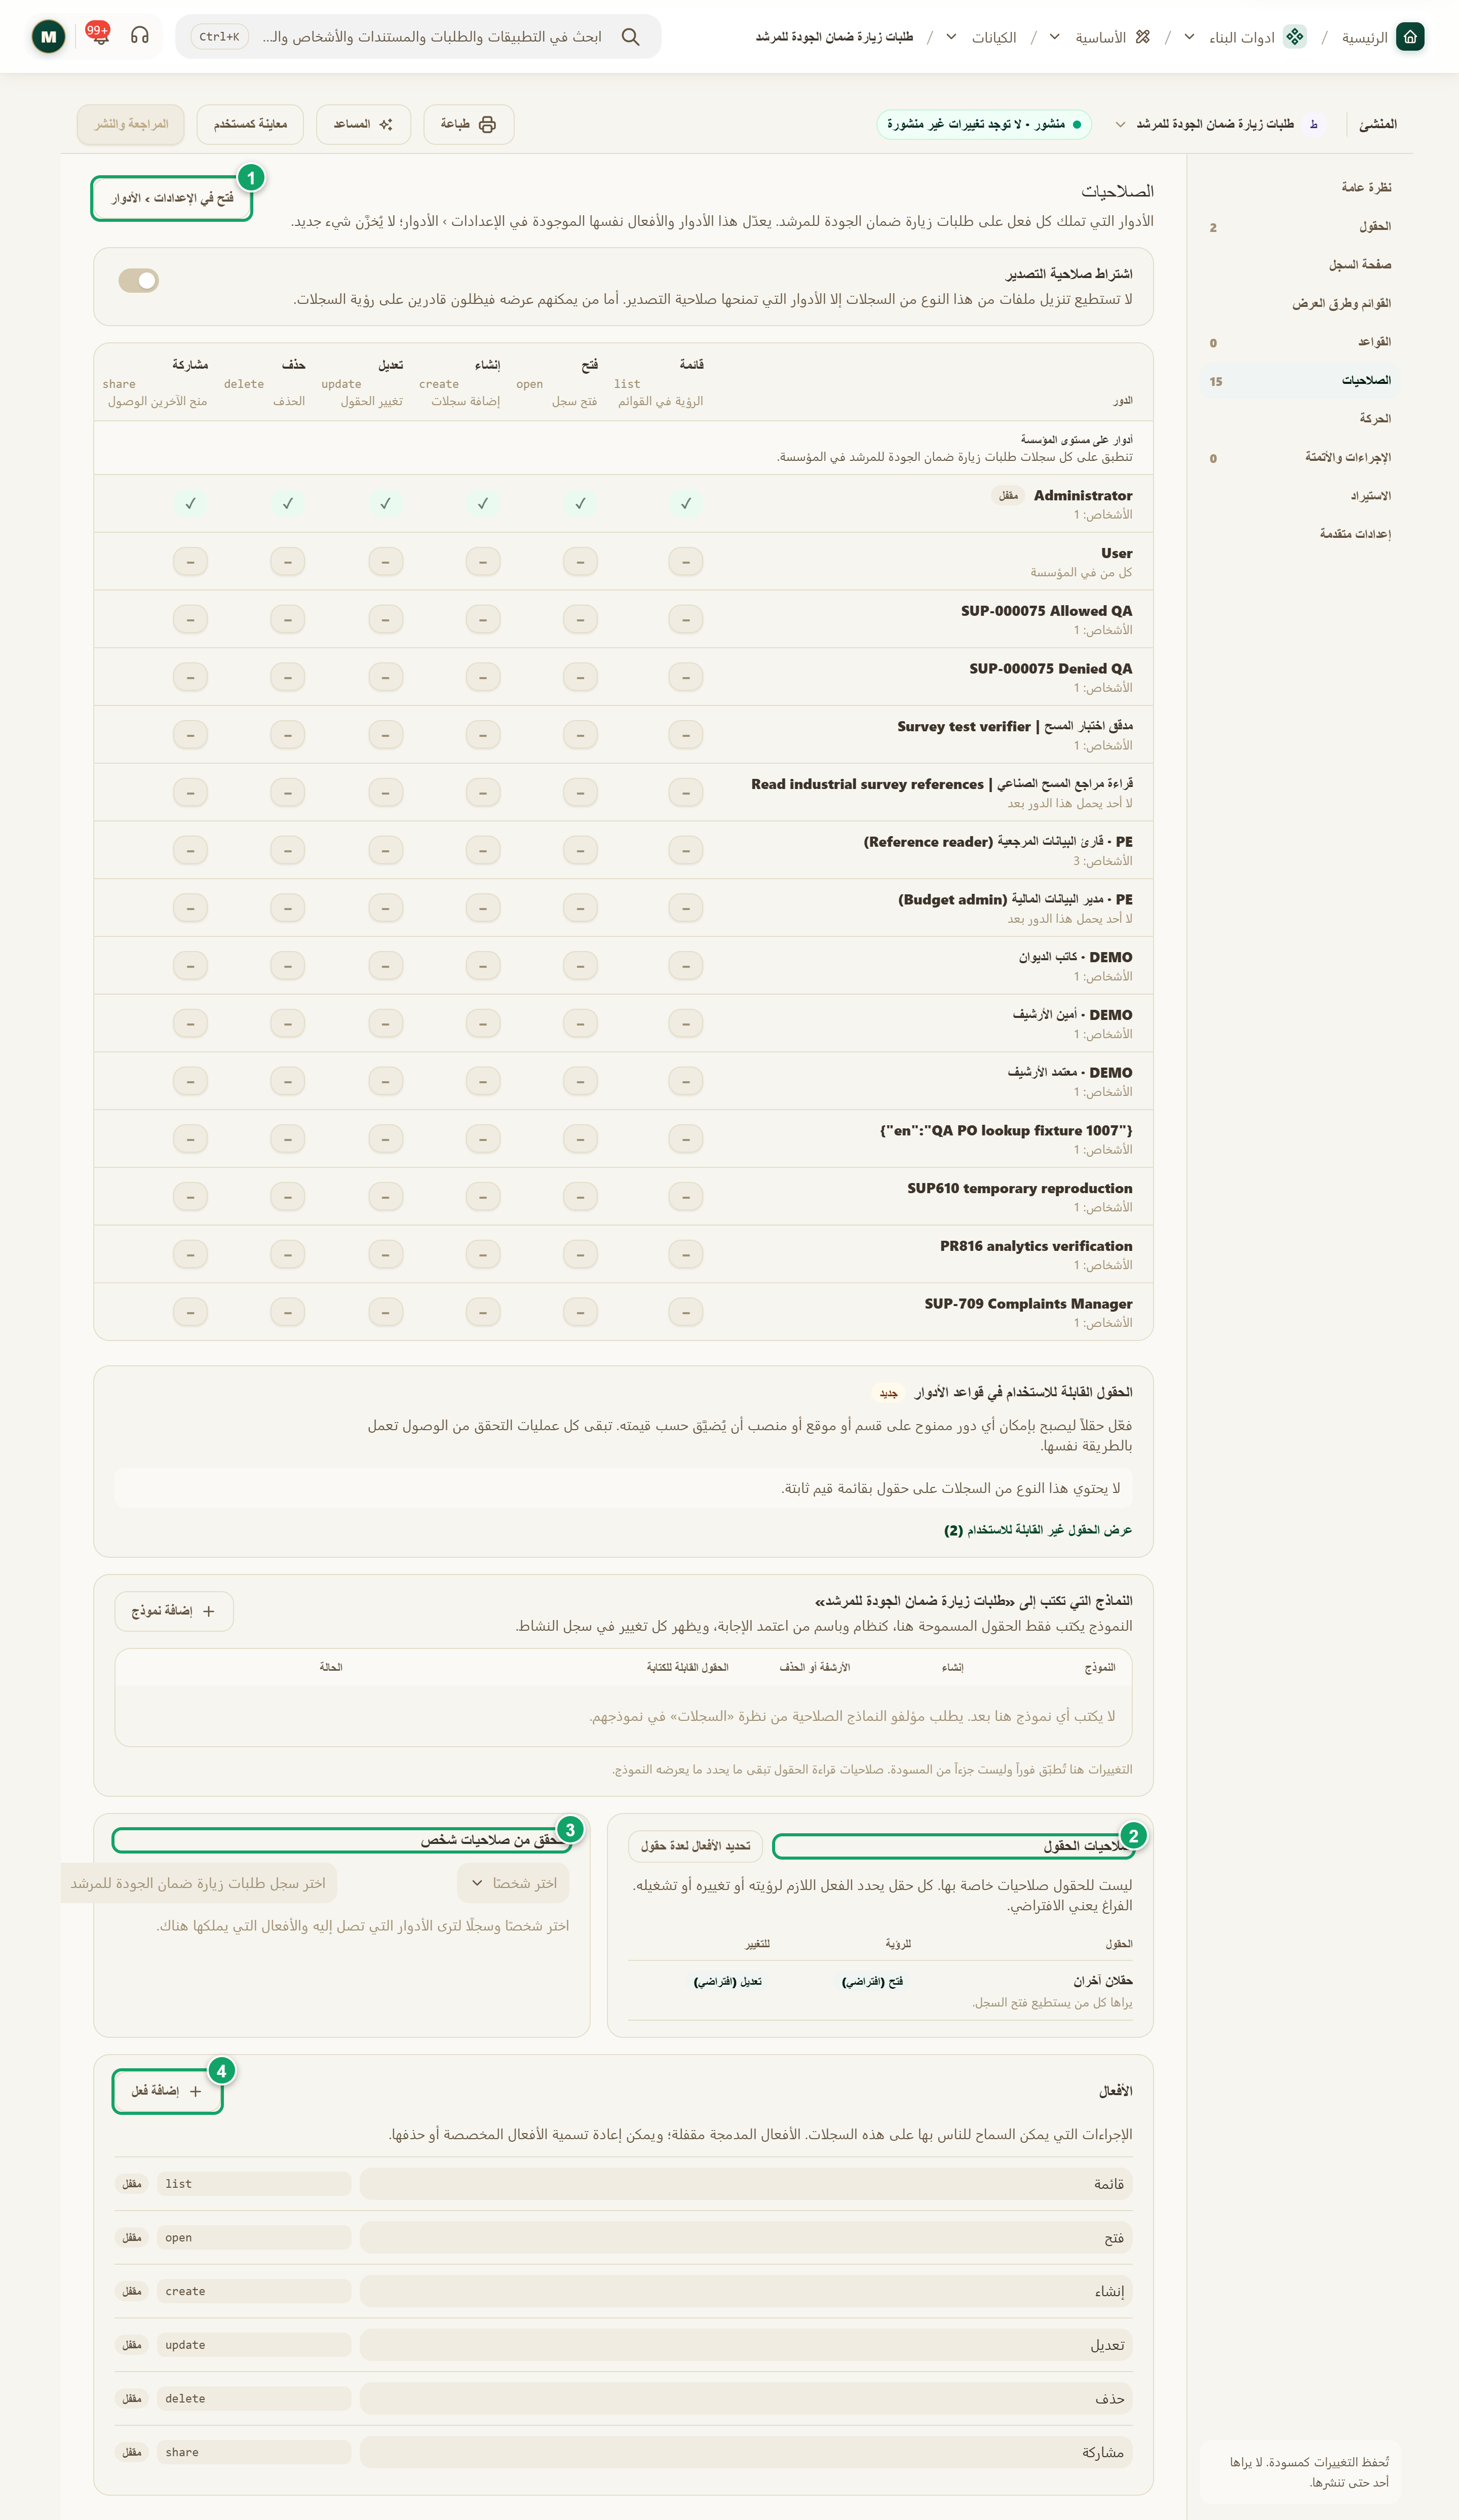
\includegraphics[width=0.95\linewidth,height=0.72\textheight,keepaspectratio]{figures/screens/ch06-ws-access-ar.png}
\caption{قسم «الصلاحيات»}
\label{fig:builder-access-screen}
\shotnote{يعرض القسم الأدوار والأفعال على هذا النوع، ثم صلاحيات الحقول وأداة فحص الوصول وقائمة الأفعال. والأدوار الظاهرة أدوار مؤسسة الاختبار. ① «فتح في الإعدادات › الأدوار». ② «صلاحيات الحقول»: تحدد الفعل اللازم لرؤية حقل أو تغييره. ③ «التحقق من صلاحيات شخص»: يبيّن ما يستطيعه شخص على سجل. ④ «إضافة فعل»: يضيف فعلاً مخصصاً مثل الاعتماد.}
\end{figure}


\begin{table}[H]
\centering
\caption{الأفعال المدمجة}
\label{tab:builder-access-verbs}
\begin{tabularx}{\linewidth}{R{3.6cm} Y}
\rcHeaderRow
\thh{الفعل} & \thh{ماذا يسمح به؟}\\
\en{list} & الرؤية في القوائم.\\
\en{open} & فتح سجل.\\
\en{create} & إضافة سجلات.\\
\en{update} & تغيير الحقول.\\
\en{delete} & الحذف.\\
\en{share} & منح الآخرين الوصول.\\
\en{export} & تنزيل ملف، ويظهر عند تفعيل «اشتراط صلاحية التصدير».\\
\end{tabularx}
\end{table}

\begin{table}[H]
\centering
\caption{ما الذي تجده هنا؟}
\label{tab:builder-access-data}
\begin{tabularx}{\linewidth}{R{3.6cm} Y}
\rcHeaderRow
\thh{البطاقة} & \thh{المحتوى والإجراء}\\
الأدوار والأفعال & اضغط الخانة لتمنح الدور فعلاً أو تسحبه. تظهر أدوار على مستوى المؤسسة، وأدوار على سجل واحد، وأدوار أخرى لها صلاحيات هنا.\\
صلاحيات الحقول & ليست للحقول صلاحيات خاصة؛ بل يحدد كل حقل الفعل اللازم «للرؤية» أو «للتغيير» أو «للتشغيل». الفراغ يعني الافتراضي.\\
الأفعال & «إضافة فعل» مخصص، مثل «اعتماد الميزانية»، ثم منحه للأدوار.\\
الحقول القابلة للاستخدام في قواعد الأدوار & تسمح بتضييق الدور حسب قيمة حقل، مثل الفرع.\\
اشتراط صلاحية التصدير & عند تفعيله لا ينزّل ملفات من هذا النوع إلا الأدوار التي تملك فعل \en{export}، ويبقى من يرى السجلات قادراً على رؤيتها.\\
النماذج التي تكتب إلى هذا النوع & تحدد النماذج المسموح لها بكتابة حقول هذا النوع. التغيير هنا يُطبّق فوراً، وليس جزءاً من المسودة.\\
التحقق من صلاحيات شخص & تختار شخصاً وسجلاً فترى الأدوار التي تصل إليه والأفعال التي يملكها.\\
\end{tabularx}
\end{table}

\begin{figure}[H]
\centering
\begin{tikzpicture}[node distance=0.5cm]
\node[entity] (role) {\RL{الدور}};
\node[entity,below=0.7cm of role] (verb) {\RL{الفعل}};
\node[entityOpt,below right=0.7cm and 0.3cm of verb] (field) {\RL{حقل يطلب الفعل}};
\node[entityOpt,below left=0.7cm and 0.3cm of verb] (records) {\RL{سجلات النوع}};
\draw[dependsOn] (role) -- (verb);
\draw[dependsOnOpt] (verb.south) -- ++(0,-0.3) -| (field.north);
\draw[dependsOnOpt] (verb.south) -- ++(0,-0.3) -| (records.north);
\end{tikzpicture}
\rclegend
\caption{من الدور إلى ما يستطيع الشخص فعله}
\label{fig:builder-access-model}
\shotnote{يوضّح الشكل أن الشخص لا يأخذ الصلاحية مباشرة، بل يأخذها من دوره، والدور يملك أفعالاً على سجلات النوع. ويمكن لحقل حساس أن يطلب فعلاً بعينه، فلا يراه أو يغيّره إلا من يملك ذلك الفعل. لذلك ابدأ بالأفعال المدمجة، ولا تضف فعلاً مخصصاً إلا لعمل له معنى مستقل مثل الاعتماد.}
\end{figure}

\subsection{خطوات العمل والتحقق}
\begin{enumerate}
\item افتح نوع السجلات واختر «الصلاحيات»، ثم راجع الأدوار الظاهرة.
\item اضغط الخانات لتمنح كل دور الأفعال التي يحتاجها عمله فقط.
\item للحقول الحساسة، افتح «صلاحيات الحقول» وحدد الفعل اللازم لرؤيتها أو تغييرها.
\item استخدم «التحقق من صلاحيات شخص» على موظف وسجل تجريبي، ثم انشر التغييرات.
\end{enumerate}

\textbf{تحقق ومعالجة المشكلة:} يجب أن تُظهر أداة التحقق الأفعال المتوقعة للشخص، وأن يرى المستخدم بعد النشر ما يخصه فقط. فإذا ظهرت رسالة «تحتاج فعل «تحديث» على الأدوار لتغيير الصلاحيات»، فاطلب ذلك من مسؤول المؤسسة؛ وإذا لم يظهر حقل لمستخدم، فراجع الفعل المطلوب له في «صلاحيات الحقول».

\clearpage
\section{صلاحيات الحقول والتحقق من صلاحيات شخص}
\label{sec:builder-feature-field-access}

تحدد صلاحيات النوع من يرى السجلات ومن يغيّرها، لكن بعض الحقول تحتاج إلى حماية أدق، مثل حقل المبلغ أو ملاحظات المراجع. وتشرح هذه الصفحة ثلاث بطاقات في قسم «الصلاحيات»: «صلاحيات الحقول» التي تحدد الفعل المطلوب لرؤية كل حقل وتغييره، و«الحقول القابلة للاستخدام في قواعد الأدوار» التي تضيّق الدور بقيمة في السجل، و«التحقق من صلاحيات شخص» التي تبيّن ما يراه شخص معيّن فعلاً.

\textbf{المسار ومن يستخدمه:} «المنشئ» ← «الصلاحيات». يستخدمه من يبني النوع بالتنسيق مع مسؤول الأدوار، لأن القسم يعدّل الأدوار والأفعال نفسها الموجودة في «الإعدادات» ← «الأدوار».

\begin{rcnote}[مثال: شركة الأفق]
يجعل المسؤول حقل «ملاحظات المراجعة» في «طلبات الزيارة» للقراءة فقط إلا لمن يملك فعل الاعتماد، ثم يستخدم «التحقق من صلاحيات شخص» مع عمر حداد وأحد طلباته، فيتأكد أن عمر يرى الملاحظات ولا يستطيع تغييرها.
\end{rcnote}

\begin{figure}[H]
\centering
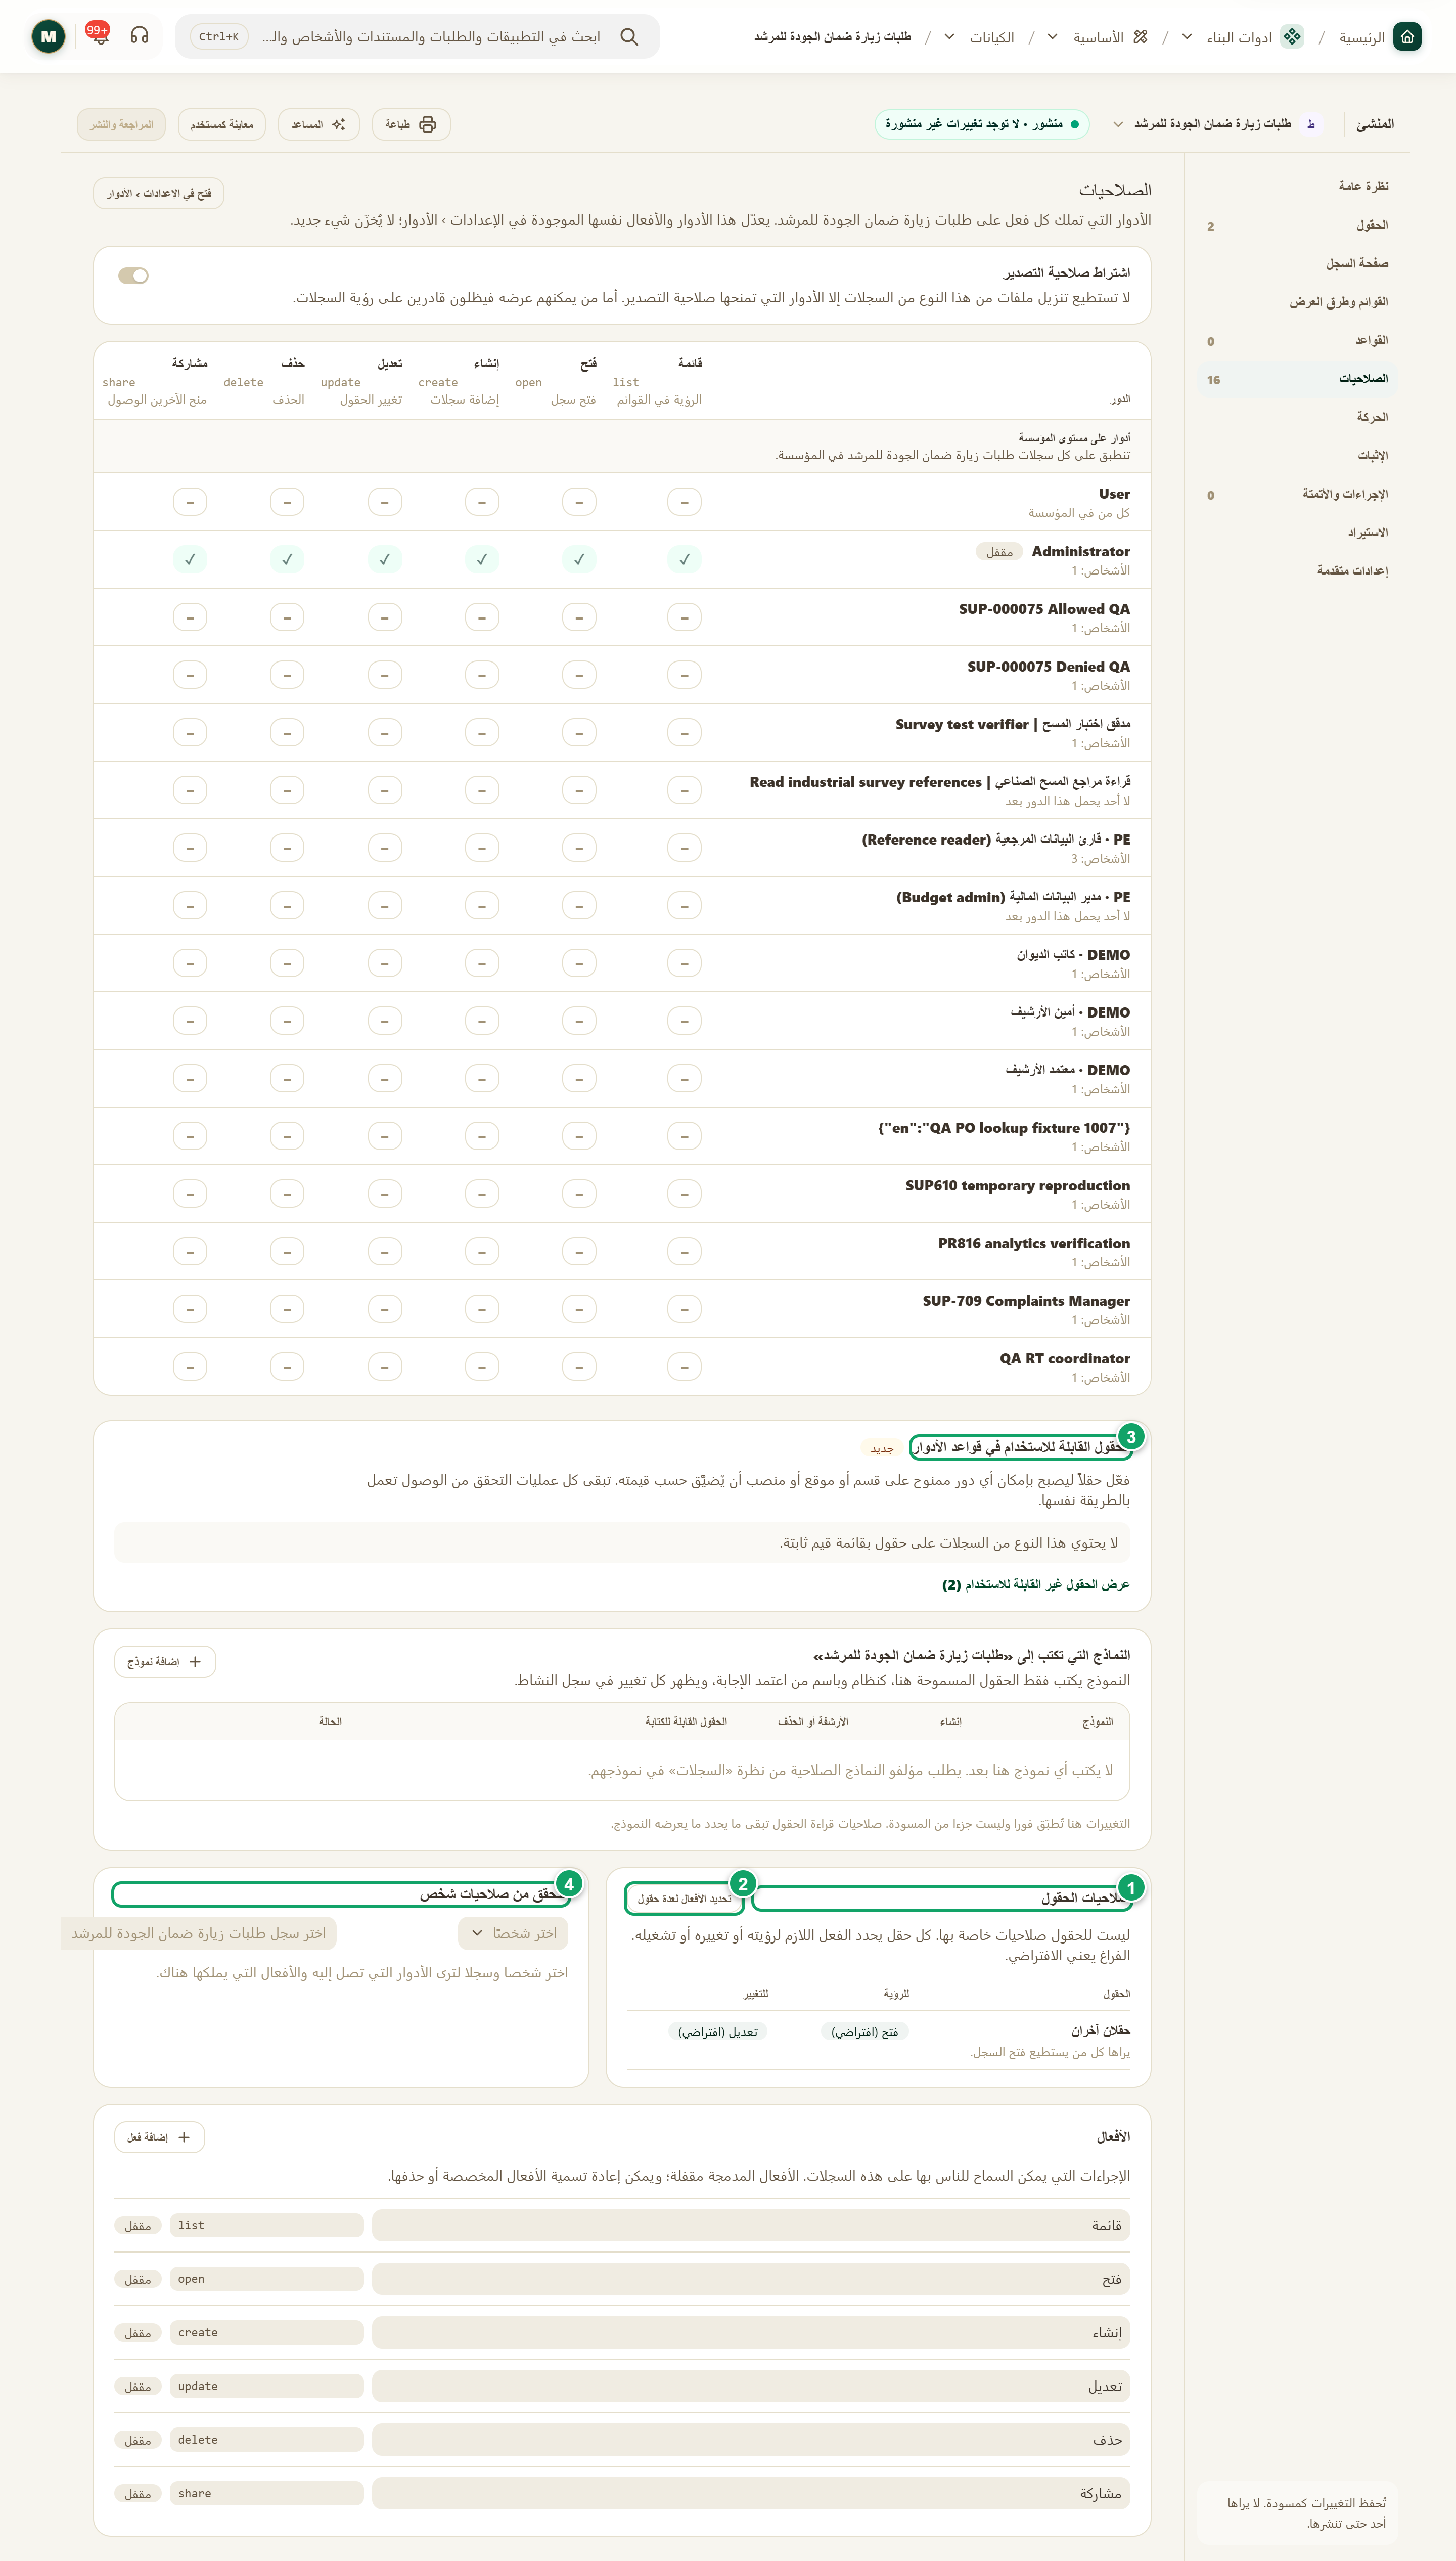
\includegraphics[width=0.95\linewidth,height=0.72\textheight,keepaspectratio]{figures/screens/ch06-ws-field-access-ar.png}
\caption{بطاقات الصلاحيات الدقيقة في قسم «الصلاحيات»}
\label{fig:builder-field-access-screen}
\shotnote{تعرض الصورة قسم «الصلاحيات» في النوع الاختباري كاملاً، ومنه البطاقات التي تضبط الحقول وتفحص ما يراه شخص معيّن. ويفيدك ذلك في معرفة ترتيبها على الصفحة قبل أن تبدأ. ① «صلاحيات الحقول»: جدول الفعل المطلوب لرؤية كل حقل وتغييره. ② «تحديد الأفعال لعدة حقول». ③ «الحقول القابلة للاستخدام في قواعد الأدوار»: تضيّق الدور بقيمة في السجل. ④ «التحقق من صلاحيات شخص»: يفحص ما يراه شخص في سجل.}
\end{figure}

\begin{table}[H]
\centering
\caption{بطاقات الصلاحيات الدقيقة}
\label{tab:builder-field-access-cards}
\begin{tabularx}{\linewidth}{R{3.6cm} Y}
\rcHeaderRow
\thh{البطاقة} & \thh{ما تقدمه}\\
صلاحيات الحقول & جدول بالحقول، لكل حقل عمودان: «للرؤية» و«للتغيير». تختار في كل منهما الفعل المطلوب، أو تتركه فارغاً ليتبع الصلاحية الافتراضية للسجل. ويعرض كل صف من يُخفى عنه الحقل ومن يراه للقراءة فقط.\\
تحديد الأفعال لعدة حقول & تختار عدة حقول وتضبط لها «للرؤية» و«للتغيير» معاً: الإبقاء على الحالي، أو الافتراضي، أو فعل معيّن، أو النظام وحده. ثم تضغط «تطبيق»، فيذهب التغيير إلى المسودة.\\
الحقول القابلة للاستخدام في قواعد الأدوار & تفعّل حقل علاقة أو قائمة أو نعم/لا، فيصبح ممكناً أن يُضيَّق الدور الممنوح على وحدة أو موقع أو منصب بقيمة هذا الحقل. ولا تصلح لذلك حقول النص والأرقام والتواريخ والحقول متعددة القيم، ويُقفل الحقل الذي تستخدمه الأدوار.\\
التحقق من صلاحيات شخص & تختار شخصاً وسجلاً، فترى الأدوار التي تصل إلى السجل، والأفعال التي يملكها، مع شطب ما لا يملكه، وعدد الحقول المخفية عنه أو المقروءة فقط. والفحص يعتمد على صلاحيات المسودة، فتتحقق قبل النشر.\\
\end{tabularx}
\end{table}

\begin{figure}[H]
\centering
\begin{tikzpicture}[node distance=0.5cm]
\node[stepBox] (a) {\RL{الأفعال على النوع}};
\node[stepBox,below=of a] (b) {\RL{صلاحيات الحقول}};
\node[stepBox,below=of b] (c) {\RL{التحقق من صلاحيات شخص}};
\node[stepBox,below=of c] (d) {\RL{المراجعة والنشر}};
\draw[flowsTo] (a) -- (b);
\draw[flowsTo] (b) -- (c);
\draw[flowsTo] (c) -- (d);
\end{tikzpicture}
\rclegend
\caption{ضبط صلاحيات الحقول والتأكد منها}
\label{fig:builder-field-access-flow}
\shotnote{يبدأ المخطط بأفعال النوع لأن صلاحية الحقل تُكتب بفعل منها، فلا معنى لها قبل أن تُمنح الأدوار أفعالها. ويضع التحقق من شخص بعينه قبل النشر، لأن الفحص يقرأ المسودة، فتكتشف الحقل المكشوف أو المخفي بالخطأ قبل أن يصل إلى الفريق.}
\end{figure}

\subsection{خطوات العمل والتحقق}
\begin{enumerate}
\item افتح «الصلاحيات»، وتأكد أن الأدوار تملك الأفعال الأساسية على النوع، مثل الفتح والتغيير.
\item في «صلاحيات الحقول» اختر للحقل الحساس الفعل المطلوب في «للرؤية» أو «للتغيير»، أو استخدم «تحديد الأفعال لعدة حقول» لعدة حقول معاً.
\item في «التحقق من صلاحيات شخص» اختر موظفاً وسجلاً، وراجع الحقول المخفية عنه والمقروءة فقط.
\item انشر التغييرات، ثم اطلب من الموظف أن يفتح السجل ويتأكد مما يراه.
\end{enumerate}

\textbf{تحقق ومعالجة المشكلة:} يجب أن يطابق ما يراه الموظف نتيجة الفحص. فإذا ظهر «لا يستطيع هذا الشخص فتح السجل»، فالمشكلة في أفعال النوع أو في دوره، لا في صلاحيات الحقول؛ فراجع الأدوار التي تصل إلى السجل أولاً.

\clearpage
\section{الإجراءات والأتمتة}
\label{sec:builder-feature-actions}

الإجراء زر يظهر في السجل، يُنشئ مستند Word أو جدول بيانات من بيانات السجل، أو يفتح رابطاً، أو يبدأ مسار عمل. ويجمع هذا القسم أزرار النوع، ويعرض الأتمتة المرتبطة به، والحقول المحسوبة التي يعيد النظام حسابها دورياً.

\textbf{المسار ومن يستخدمه:} نوع السجلات ← «الإجراءات والأتمتة». يستخدمه من يبني النوع بعد تجهيز القالب أو مسار العمل الذي سيستدعيه الزر.

\begin{rcnote}[مثال: شركة الأفق]
يضيف مسؤول النظام إلى طلب الزيارة زراً من نوع «مستند Word» يُنشئ خطاب تأكيد الزيارة من بيانات الطلب، ويجعله متاحاً لمن يملك فعل الاعتماد فقط. ويبدأ الزر من ①.
\end{rcnote}

\begin{figure}[H]
\centering
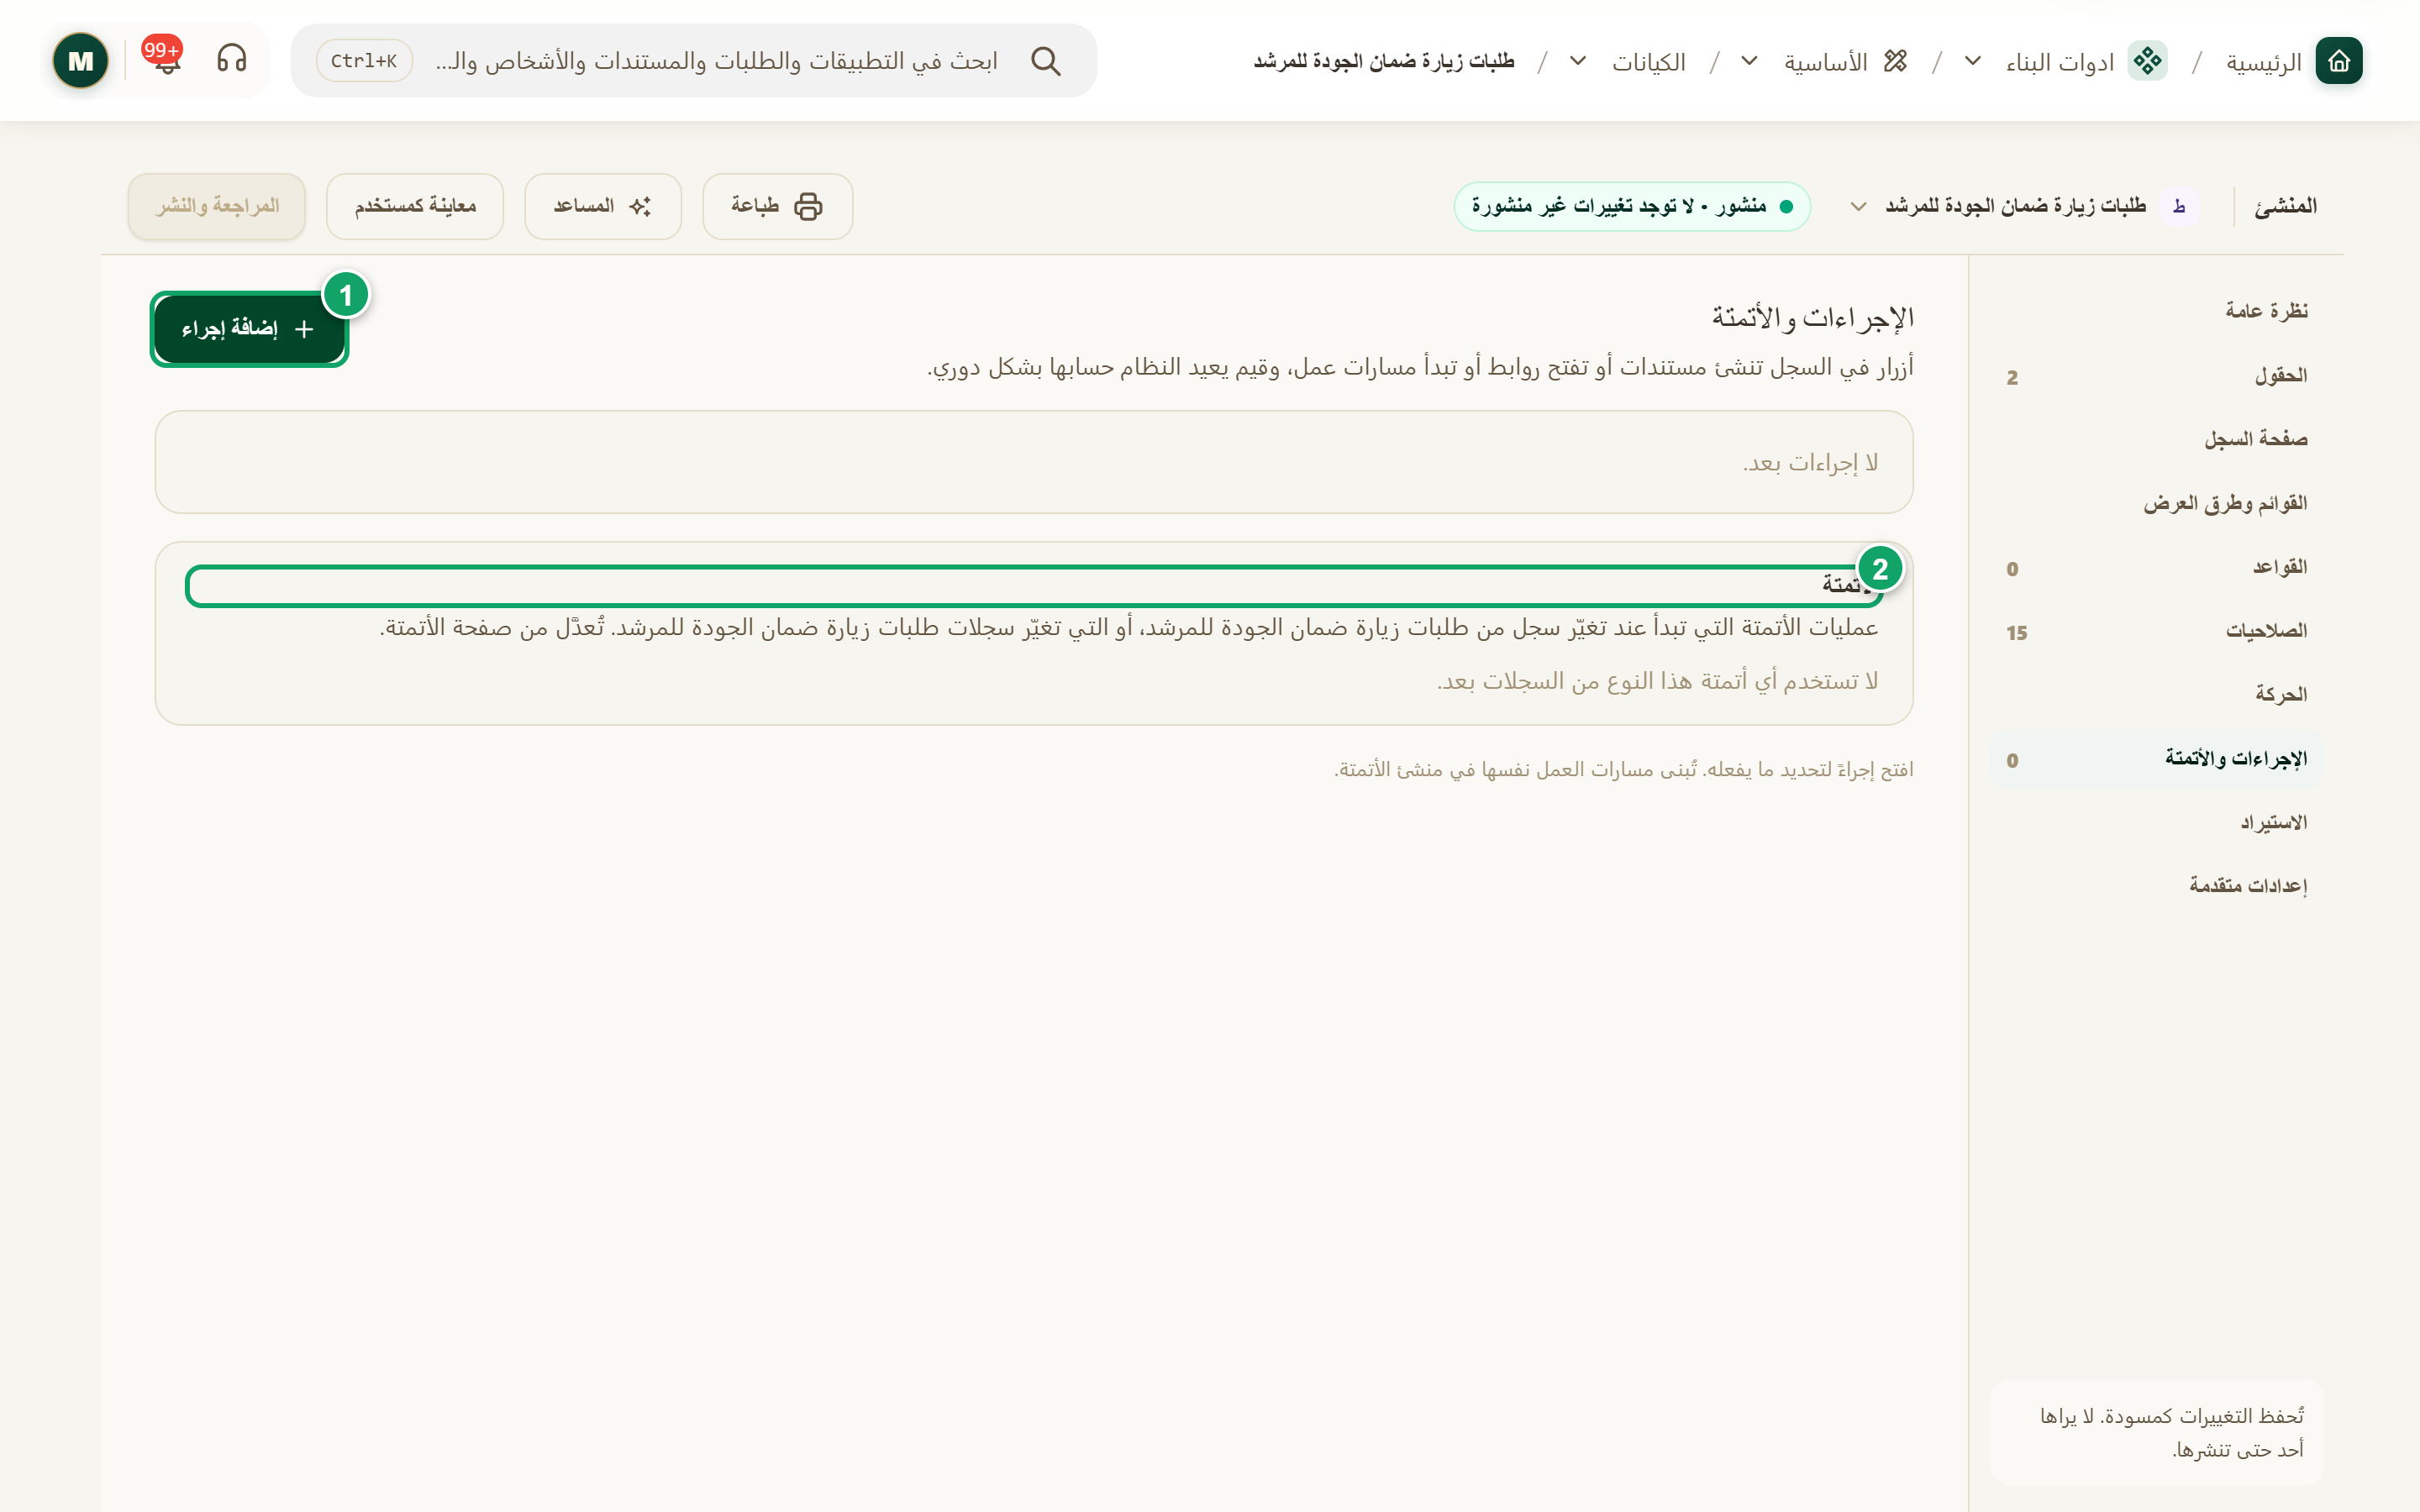
\includegraphics[width=0.95\linewidth,height=0.72\textheight,keepaspectratio]{figures/screens/ch06-ws-actions-ar.png}
\caption{قسم «الإجراءات والأتمتة»}
\label{fig:builder-actions-screen}
\shotnote{يعرض القسم أزرار النوع والأتمتة المرتبطة به، وهما فارغان في النوع الاختباري. ① «إضافة إجراء»: يُنشئ زراً جديداً ويفتحه لتحدد ما يفعله. ② «الأتمتة»: قائمة للاطلاع على الأتمتة التي تبدأ بتغيّر سجلات النوع أو تغيّرها.}
\end{figure}


\begin{table}[H]
\centering
\caption{ما الذي تجده هنا؟}
\label{tab:builder-actions-data}
\begin{tabularx}{\linewidth}{R{3.6cm} Y}
\rcHeaderRow
\thh{الجزء} & \thh{المحتوى والإجراء}\\
الإجراءات & لكل إجراء نوعه: «مستند Word» أو «جدول بيانات» أو «رابط» أو «مسار عمل»، ومن يستطيع تشغيله: «يتطلب» فعلاً معيناً، أو «كل من يستطيع تغيير السجل».\\
إضافة إجراء & يُنشئ «إجراء جديد» في المسودة ويفتحه في «الحقول»، حيث تختار ما يفعله والقالب أو المسار الذي يستخدمه.\\
الأتمتة & قائمة للاطلاع بالأتمتة التي «تبدأ عند التغيير» في سجل من هذا النوع، أو التي «تغيّر السجلات»، مع حالتها: «منشورة» أو «غير منشورة» أو «متوقفة مؤقتًا». تُعدَّل من صفحة الأتمتة.\\
يُعاد حسابه دوريًا & الحقول المحسوبة التي يعيد النظام حسابها «يوميًا» أو «أسبوعيًا» أو «شهريًا»، وتظهر عند وجودها فقط.\\
\end{tabularx}
\end{table}

\begin{figure}[H]
\centering
\begin{tikzpicture}[node distance=0.5cm]
\node[entity] (action) {\RL{زر الإجراء في السجل}};
\node[entityOpt,below right=0.7cm and 0.3cm of action] (tpl) {\RL{قالب مستند}};
\node[entityOpt,below left=0.7cm and 0.3cm of action] (sop) {\RL{مسار عمل}};
\draw[dependsOnOpt] (action.south) -- ++(0,-0.3) -| (tpl.north);
\draw[dependsOnOpt] (action.south) -- ++(0,-0.3) -| (sop.north);
\end{tikzpicture}
\rclegend
\caption{ما يستدعيه الإجراء}
\label{fig:builder-actions-model}
\shotnote{يوضّح الشكل أن الزر لا يعمل وحده، بل يستدعي شيئاً جاهزاً: قالب مستند تُعدّه في صفحات القوالب، أو مسار عمل تبنيه في الأتمتة. لذلك جهّز القالب أو المسار أولاً، ثم أنشئ الإجراء واربطه به.}
\end{figure}

\subsection{خطوات العمل والتحقق}
\begin{enumerate}
\item جهّز القالب أو مسار العمل الذي سيستدعيه الزر.
\item افتح نوع السجلات واختر «الإجراءات والأتمتة»، ثم اضغط «إضافة إجراء».
\item في الحقل الذي يُفتح، سمِّ الإجراء واختر نوعه والقالب أو المسار، ثم حدد الفعل اللازم لتشغيله.
\item انشر التغييرات، ثم افتح سجلاً تجريبياً واضغط الزر.
\end{enumerate}

\textbf{تحقق ومعالجة المشكلة:} يجب أن يظهر الزر في السجل لمن يملك الفعل المطلوب، وأن ينتج المستند أو يبدأ المسار. فإذا ظهر الإجراء بنوع «غير مضبوط»، فافتحه وأكمل اختيار ما يفعله؛ وإذا لم يظهر الزر لمستخدم، فراجع الفعل الذي يتطلبه.

\clearpage
\section{الحركة}
\label{sec:builder-feature-movement}

الحركة إعداد متخصص لسجلات تنقل مبلغاً أو كمية من سجل إلى آخر، مثل التحويل بين بنود الموازنة أو بين المستودعات. فكل سجل يحدد من أين يأتي المبلغ وإلى أين يذهب، ويحافظ كيان على تساوي الطرفين، ويرحّلهما معاً عندما يصل السجل إلى حالة تختارها. ولا تحتاج معظم أنواع السجلات إلى هذا القسم. وإذا شغّلت «الإثبات» على النوع نفسه، فيجب أن ترحّل الحركة عند حالة التدقيق، كما تشرح الصفحة \ref{sec:builder-feature-evidence}.

\textbf{المسار ومن يستخدمه:} نوع السجلات ← «الحركة». يستخدمه من يبني أنواع سجلات مالية أو مخزنية.

\begin{rcnote}[مثال: شركة الأفق]
لا يحتاج نوع «طلبات الزيارة» إلى الحركة. لكن لو أنشأت الأفق نوعاً لتحويل مبالغ بين بنود موازنة الفروع، فسيرحّل كل تحويل معتمد المبلغ من بند حلب إلى بند دمشق في خطوة واحدة. ولا يتجاوز مسؤول النظام شروط ② لأن نوع الطلبات لا يحتاج إليها.
\end{rcnote}

\begin{figure}[H]
\centering
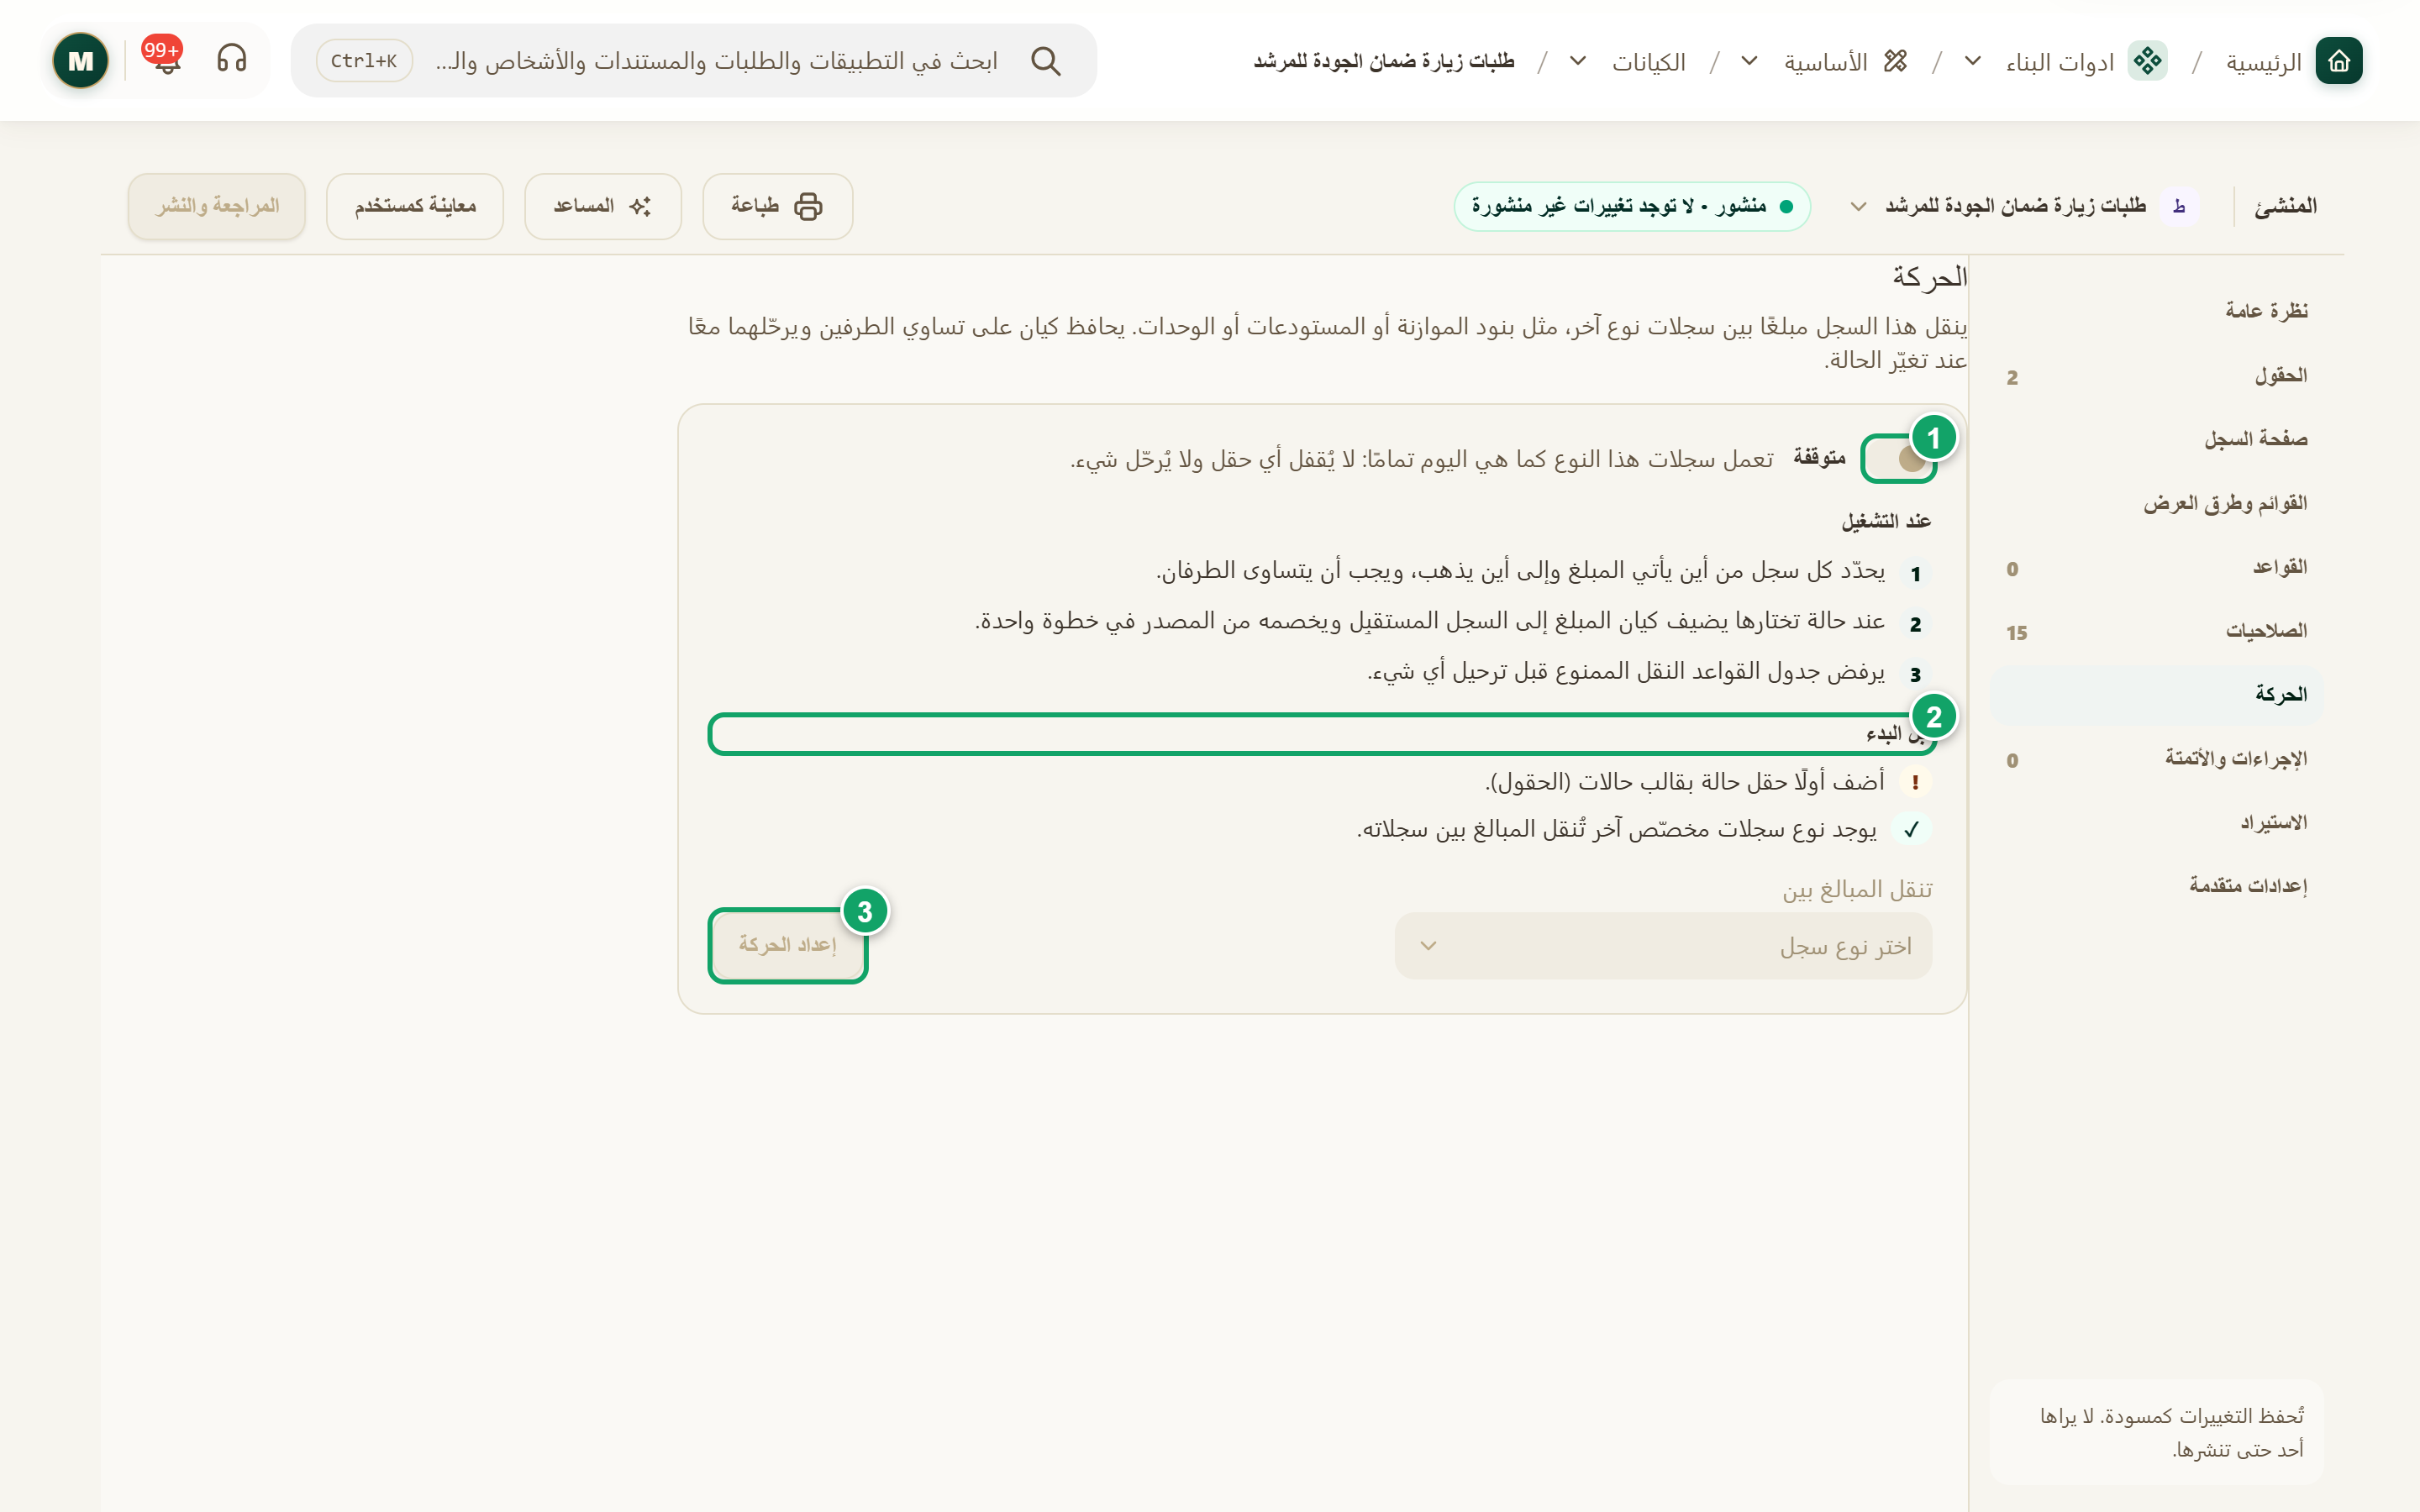
\includegraphics[width=0.95\linewidth,height=0.72\textheight,keepaspectratio]{figures/screens/ch06-ws-movement-ar.png}
\caption{قسم «الحركة» وهي متوقفة}
\label{fig:builder-movement-screen}
\shotnote{يشرح القسم ما تفعله الحركة عند تشغيلها، ويتحقق من شروطها قبل البدء. وتظهر علامة التنبيه لأن النوع الاختباري بلا حقل حالة. ① مفتاح التشغيل: متوقف، فلا يُرحَّل شيء. ② «قبل البدء»: الشروط الواجب توفرها، مع علامة لكل شرط. ③ «إعداد الحركة»: يبدأ الإعداد بعد اختيار النوع الذي تُنقل المبالغ بين سجلاته.}
\end{figure}


\begin{table}[H]
\centering
\caption{ما الذي تحتاجه وتضبطه؟}
\label{tab:builder-movement-data}
\begin{tabularx}{\linewidth}{R{3.6cm} Y}
\rcHeaderRow
\thh{الجزء} & \thh{المعنى}\\
قبل البدء & حقل «الحالة» بقالب حالات في هذا النوع، ونوع سجلات مخصّص آخر تُنقل المبالغ بين سجلاته، فيه حقلان رقميان لـ«الوارد» و«الصادر». ولا تعمل الحركة على الأنواع المدمجة.\\
الطرفان & من أين يأتي المبلغ وإلى أين يذهب، ويجب أن يتساويا.\\
الترحيل & الحالة التي يُرحَّل عندها المبلغ، وأثرها: حجز أو ترحيل أو فكّ الحجز أو عكس.\\
القواعد & ترفض النقل الممنوع قبل ترحيل أي شيء.\\
المجاميع الدورية وجرّب & تعرض المجاميع لكل فترة، وتختبر الإعداد قبل النشر.\\
\end{tabularx}
\end{table}

\begin{figure}[H]
\centering
\begin{tikzpicture}[node distance=0.5cm]
\node[stepBox] (a) {\RL{سجل الحركة: مسودة}};
\node[stepBox,below=of a] (b) {\RL{الوصول إلى حالة الترحيل}};
\node[stepBox,below=of b] (c) {\RL{خصم من المصدر وإضافة للمستقبِل}};
\draw[flowsTo] (a) -- (b);
\draw[flowsTo] (b) -- (c);
\end{tikzpicture}
\rclegend
\caption{متى يتحرك المبلغ؟}
\label{fig:builder-movement-flow}
\shotnote{يبيّن المخطط أن المبلغ لا يتحرك عند إنشاء السجل، بل عندما يصل إلى الحالة التي اخترتها للترحيل. وعندها يُخصم من المصدر ويُضاف إلى المستقبِل معاً، فلا يبقى طرف دون الآخر.}
\end{figure}

\subsection{خطوات العمل والتحقق}
\begin{enumerate}
\item تأكد من وجود حقل «الحالة» ونوع السجلات المستقبِل بحقلي الوارد والصادر.
\item افتح «الحركة»، واختر النوع من «تنقل المبالغ بين»، ثم اضغط «إعداد الحركة».
\item اضبط تبويبات «الطرفان» و«الترحيل» و«القواعد»، ثم استخدم «جرّب» قبل النشر.
\end{enumerate}

\textbf{تحقق ومعالجة المشكلة:} بعد النشر انقل سجلاً تجريبياً إلى حالة الترحيل، وتأكد من تغيّر رصيدي الطرفين بالمقدار نفسه. وإذا أوقفت الحركة لاحقاً، فتبقى المبالغ المرحّلة كما هي، ويتوقف ترحيل السجلات الجديدة فقط.

\clearpage
\section{الإثبات}
\label{sec:builder-feature-evidence}

«الإثبات» قسم متخصص لأنواع السجلات التي تسجّل مبلغاً صُرف أو قُبض، مثل مطالبات المصاريف، ويجب أن تثبته وثائق. ويسمّي القسم كل سجل من هذا النوع «قيداً»: يرفق مقدّمه الوثائق المطلوبة ثم يقدّمه، فيفحص كيان الوثائق والتكرار ويرقّم القيد ويجمّد ملفاته. ثم يجيب مدقق عن قائمة تحقق لكل وثيقة، ولا يكون المدقق منشئ القيد ولا مقدّمه. وبعد التدقيق يُقفل القيد على الجميع، ويكون التصحيح بقيد عكسي لا بالتعديل.

يبدأ القسم بحالة «متوقف»، فتعمل السجلات كما هي دون فحص أي ملف. ولا يعمل زر «تشغيل» إلا بشرطين يعرضهما القسم في «قبل أن تبدأ»: حقل حالة بقالب حالات، وحقل رقمي للمبلغ. ولا يتاح الإثبات لأنواع السجلات المدمجة في النظام.

\textbf{المسار ومن يستخدمه:} «المنشئ» ← «الإثبات». يضبطه من يبني الأنواع المالية بالتنسيق مع المسؤول المالي. وبعد النشر يظهر في صفحة السجل تبويب «الإثبات»، فيرفع فيه المقدّم الوثائق ويضغط «تقديم للتدقيق»، ويدقق فيه المدقق القيد أو يعيده للتصحيح.

\begin{rcnote}[مثال: شركة الأفق]
لا يحتاج نوع «طلبات الزيارة» إلى الإثبات لأنه لا يسجّل مبلغاً. لكن لو أنشأت الأفق نوعاً لمصاريف الزيارات، لجعل مسؤول النظام فيه وثيقة «فاتورة الفندق» مطلوبة دائماً، مع بند تحقق «الفاتورة باسم الشركة». فيرفع عمر حداد فاتورة زيارته إلى فرع حلب ويقدّم القيد، ثم تدققه سارة الخطيب.
\end{rcnote}

\begin{figure}[H]
\centering
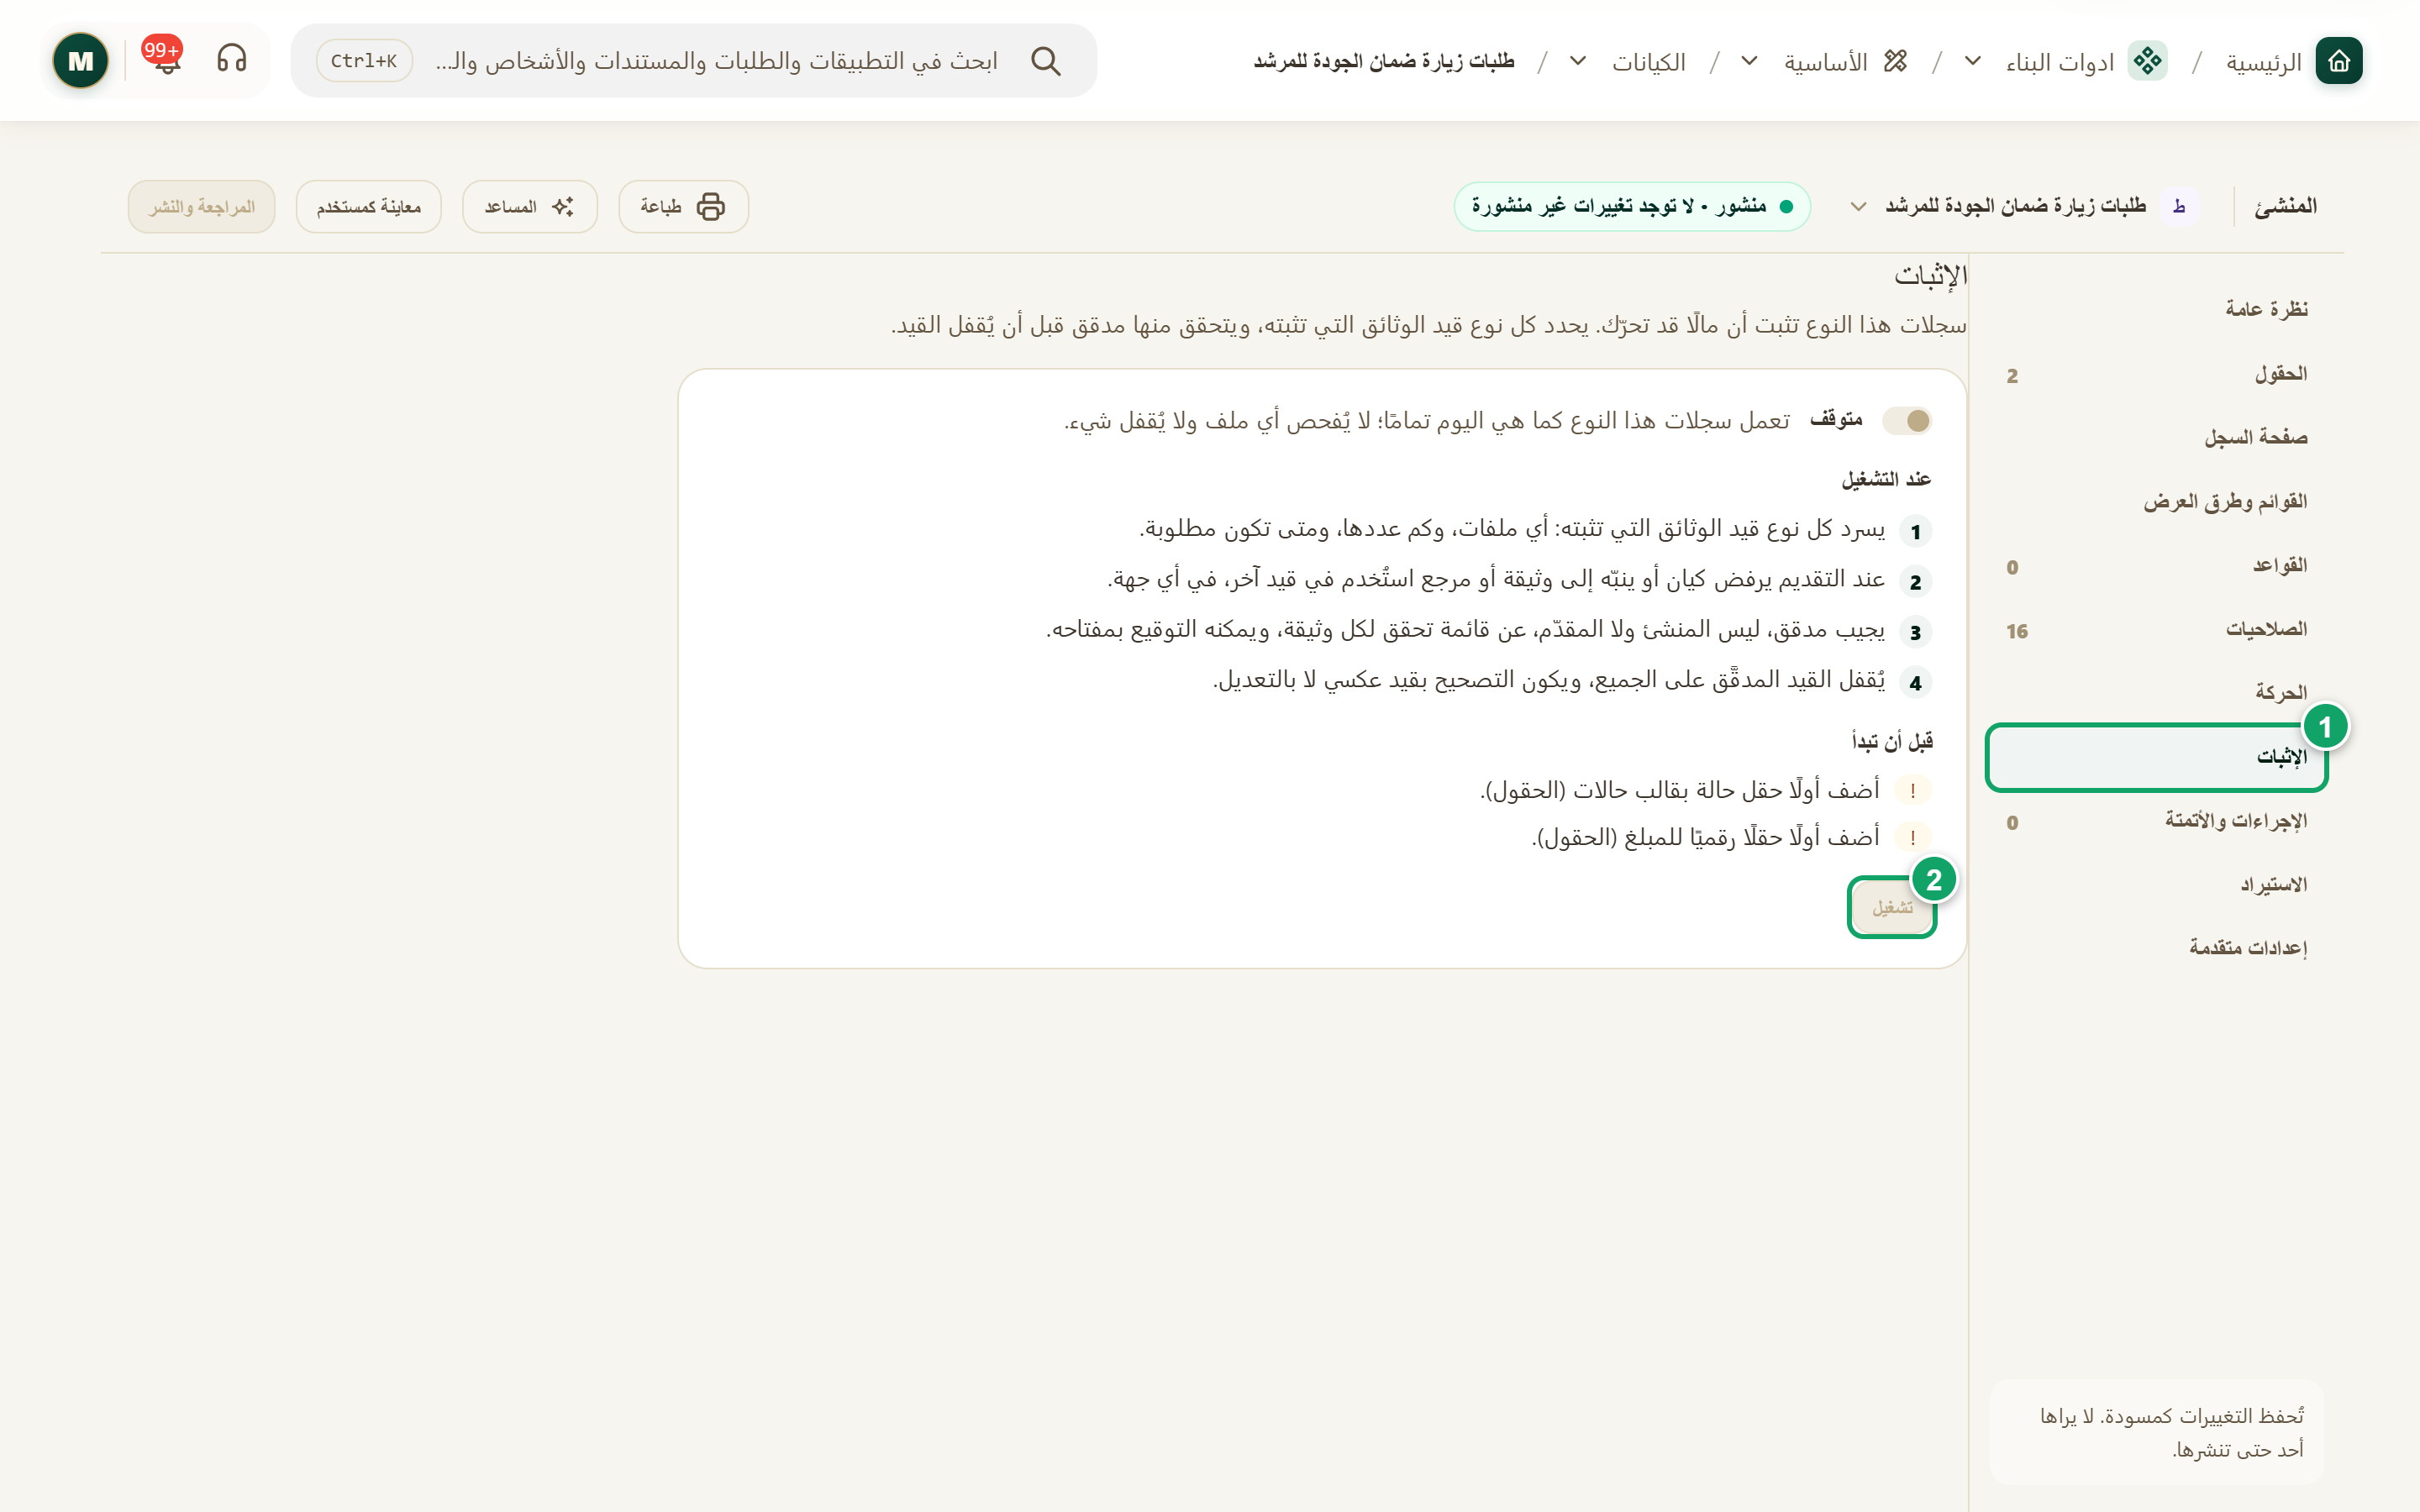
\includegraphics[width=0.95\linewidth,height=0.72\textheight,keepaspectratio]{figures/screens/ch06-ws-evidence-ar.png}
\caption{قسم «الإثبات» قبل تشغيله في نوع سجلات اختباري}
\label{fig:builder-evidence-screen}
\shotnote{تعرض الصورة القسم في النوع الاختباري على test2 وهو «متوقف»، مع شرح ما يحدث عند التشغيل وقائمة «قبل أن تبدأ». ويبيّن ذلك أن الزر يبقى معطلاً حتى يكتمل الشرطان، لأن هذا النوع لا يحوي حقل حالة ولا حقلاً رقمياً للمبلغ. ① «الإثبات» في القائمة الجانبية. ② «تشغيل»: يفعّل الإثبات بعد استيفاء الشروط.}
\end{figure}

\begin{table}[H]
\centering
\caption{تبويبات «الإثبات» بعد التشغيل}
\label{tab:builder-evidence-tabs}
\begin{tabularx}{\linewidth}{R{3.6cm} Y}
\rcHeaderRow
\thh{التبويب} & \thh{ما تضبطه فيه}\\
أنواع القيود والوثائق & في «عام»: «حقل الحالة» و«حالة التقديم» و«حالة التدقيق» و«حالات الإعادة»، و«حقل نوع القيد» عندما تختلف الوثائق حسب نوع القيد، و«حقول القيد» (المبلغ إلزامي، والعملة وتاريخ القيمة والجهة والطرف المقابل اختيارية)، و«الترقيم» ببادئة. ثم أنواع القيود، ولكل نوع «الفحوص المتقاطعة» و«وثائق الإثبات».\\
التكرار & قواعد تقارن كل قيد مقدَّم بقيود النوع حسب «محتوى الملف» أو «الحقول» أو «القراءة الآلية»، في «الجهة نفسها» أو «المؤسسة كلها»، ثم تختار «رفض» أو «تنبيه مع سبب» أو «إشارة للمدقق». وعند تطابق أكثر من قاعدة تغلب النتيجة الأشد.\\
القراءة الآلية & تقرأ الآلة من الوثائق قيماً مثل «المبلغ الإجمالي» و«رقم الوثيقة»، فتقترحها أو تقارنها بما أدخله المقدّم، ضمن «السقف الشهري» و«الصفحات لكل ملف».\\
الترحيل & يعرض «دورة الحياة» من التقديم إلى الإعادة أو التدقيق، ويفحص قالب الحالات وتوافقه مع قسم «الحركة». ودون إعداد للحركة تُثبت القيود وتُدقَّق ولا يتحرك أي مبلغ.\\
السرية & «المستوى الافتراضي» للوثائق، و«توقيع المدقق» بمفتاح العضو، و«قابلة للتعديل بعد التدقيق» للحقول التي تبقى مفتوحة بعد القفل، مثل الملاحظات. أما وثائق المستوى «سري (3)» فما فوق فتُعرض فقط، ولا تُنزَّل ولا تُرسل إلى القراءة الآلية.\\
\end{tabularx}
\end{table}

\begin{table}[H]
\centering
\caption{إعدادات كل وثيقة}
\label{tab:builder-evidence-slot}
\begin{tabularx}{\linewidth}{R{3.6cm} Y}
\rcHeaderRow
\thh{الإعداد} & \thh{المعنى}\\
مطلوبة & «دائمًا»، أو «اختيارية»، أو «عندما…» يتحقق شرط يُفحص عند التقديم ثم عند التدقيق.\\
الملفات & الصيغ المقبولة: \en{PDF} والصور و\en{Word} و\en{Excel}، وعدد الملفات «على الأقل» و«على الأكثر»، و«الحجم الأقصى (ميغابايت)»، وحد أدنى لدقة الصور. وإذا لم تختر صيغة، فتُقبل ملفات \en{PDF} والصور.\\
وثيقة مشتركة & «يمكن أن تثبت قيودًا أخرى» عندما تغطي وثيقة واحدة أكثر من قيد، مثل الأقساط.\\
السرية والقراءة & مستوى سرية خاص بالوثيقة، و«تُقرأ هذه الوثيقة آليًا».\\
قائمة تحقق المدقق & بنود يجيب عنها المدقق بنعم أو لا أو لا ينطبق مع ملاحظة، ولا يكتمل التدقيق إلا إذا كانت كل الإجابات نعم أو لا ينطبق.\\
\end{tabularx}
\end{table}

\begin{rcwarn}[الإيقاف لا يمحو ما قُدّم]
إذا أوقفت الإثبات بعد تقديم قيود، فيحتفظ كيان بإعداده ويعرض القسم «متوقف» مع زر «إعادة التشغيل»، ويبقى سجل القيود وأقفالها كما هي. ولا تُحذف ملفات الإثبات أبداً، فحتى القيد المعاد يحتفظ بملفاته القديمة بجانب الجديدة.
\end{rcwarn}

\subsection{قوائم التحقق بالأدلة}

يناسب «الإثبات» القيود المالية فقط. أما إذا أردت قائمة بنود يُجاب عنها داخل السجل، ويحتاج بعضها إلى صورة أو ملف دليلاً، مثل قائمة تحقق زيارة، فاجعلها سجلات مرتبطة واضبطها من حقل «علاقة» في نوع البنود: اختر «عرض العلاقة في التبويب»، ثم «قائمة تحقق» في «طريقة عرض العلاقات». وبعد ذلك تحدد «حقل الإجابة»، وتختار ضمن «ملفات الأدلة» قيمة «مجموعة الملفات» التي تُرفع إليها الأدلة، وتضيف شرطاً في «الأدلة مطلوبة فقط عندما…» إن لزم.

\begin{figure}[H]
\centering
\begin{tikzpicture}[node distance=0.5cm]
\node[stepBox] (a) {\RL{حقل حالة وحقل مبلغ}};
\node[stepBox,below=of a] (b) {\RL{تشغيل الإثبات}};
\node[stepBox,below=of b] (c) {\RL{أنواع القيود والوثائق}};
\node[stepBox,below=of c] (d) {\RL{التكرار والسرية}};
\node[stepBox,below=of d] (e) {\RL{الترحيل مع الحركة}};
\node[stepBox,below=of e] (f) {\RL{المراجعة والنشر}};
\draw[flowsTo] (a) -- (b);
\draw[flowsTo] (b) -- (c);
\draw[flowsTo] (c) -- (d);
\draw[flowsTo] (d) -- (e);
\draw[flowsTo] (e) -- (f);
\end{tikzpicture}
\rclegend
\caption{تشغيل الإثبات وضبطه}
\label{fig:builder-evidence-flow}
\shotnote{يبدأ المخطط بالحقلين لأن زر التشغيل يبقى معطلاً دونهما، ولأن كيان يستنتج منهما حالات التقديم والتدقيق وحقل المبلغ. ويأتي الترحيل قبل النشر لأن كيان يرفض النشر إذا لم يتوافق الإثبات مع إعداد «الحركة»، فالمال لا يتحرك إلا بعد التدقيق.}
\end{figure}

\subsection{خطوات العمل والتحقق}
\begin{enumerate}
\item تأكد في «الحقول» من وجود حقل «الحالة» بـ«قالب ثابت» منشور فيه حالة للتقديم وأخرى للتدقيق، ومن وجود حقل «رقم» للمبلغ.
\item افتح «الإثبات» واضغط «تشغيل»، ثم راجع في «عام» الحالات التي اقترحها كيان، واختر «حقول القيد» و«البادئة».
\item في «وثائق الإثبات» اضغط «إضافة وثيقة» لكل وثيقة، وحدد «مطلوبة» والملفات، ثم أضف بنود «قائمة تحقق المدقق» بزر «إضافة بند».
\item راجع «التكرار» و«السرية»، ثم افتح «الترحيل» وعالج كل فحص لم يتحقق، ولا سيما إذا كان للنوع إعداد في «الحركة».
\item انشر التغييرات، ثم أنشئ سجلاً تجريبياً، وارفع وثائقه من تبويب «الإثبات»، واضغط «تقديم للتدقيق»، واطلب من مستخدم آخر أن يدققه.
\end{enumerate}

\textbf{تحقق ومعالجة المشكلة:} يجب أن تظهر شارة «جاهز» بجانب عنوان القسم، وأن يحمل القيد المقدَّم رقماً يبدأ ببادئتك. فإذا بقي زر «تشغيل» معطلاً، فأضف الحقل الذي تشير إليه «قبل أن تبدأ». وإذا ظهرت شارة بعدد المشكلات «للإصلاح» أو مشكلة «إعداد الإثبات» في «قبل النشر»، فافتح التبويب المعلَّم بالخطأ وأكمل ما ينقصه.

\clearpage
\section{الاستيراد}
\label{sec:builder-feature-import}

يحدد قسم «الاستيراد» كيف يحمّل الناس سجلات هذا النوع ويحدّثونها من ملفات Excel وCSV. وأهم ما فيه «مفاتيح الاستيراد»: حقل أو مجموعة حقول، مثل رمز أو رقم، يطابق بها كيان كل صف في الملف مع سجل موجود، فيحدّثه بدلاً من أن ينشئ نسخة مكررة. وعندما يكون الخيار متوقفاً، يعمل الاستيراد كالمعتاد ويخمّن المطابقة بالمعرّف أو الرمز أو الاسم.

\textbf{المسار ومن يستخدمه:} نوع السجلات ← «الاستيراد». يستخدمه من يبني نوع السجلات، قبل أن يبدأ الفريق تحديث السجلات من ملفات.

\begin{rcnote}[مثال: شركة الأفق]
يضيف مسؤول النظام مفتاح استيراد مبنياً على رقم الطلب \en{HZN-VR-0001}، فيرفع عمر حداد ملف Excel بمواعيد الزيارات المعدّلة، ويحدّث كيان الطلبات الموجودة نفسها دون إنشاء طلبات جديدة. ويضيف المفتاح من ② ثم يفحصه من ③.
\end{rcnote}

\begin{figure}[H]
\centering
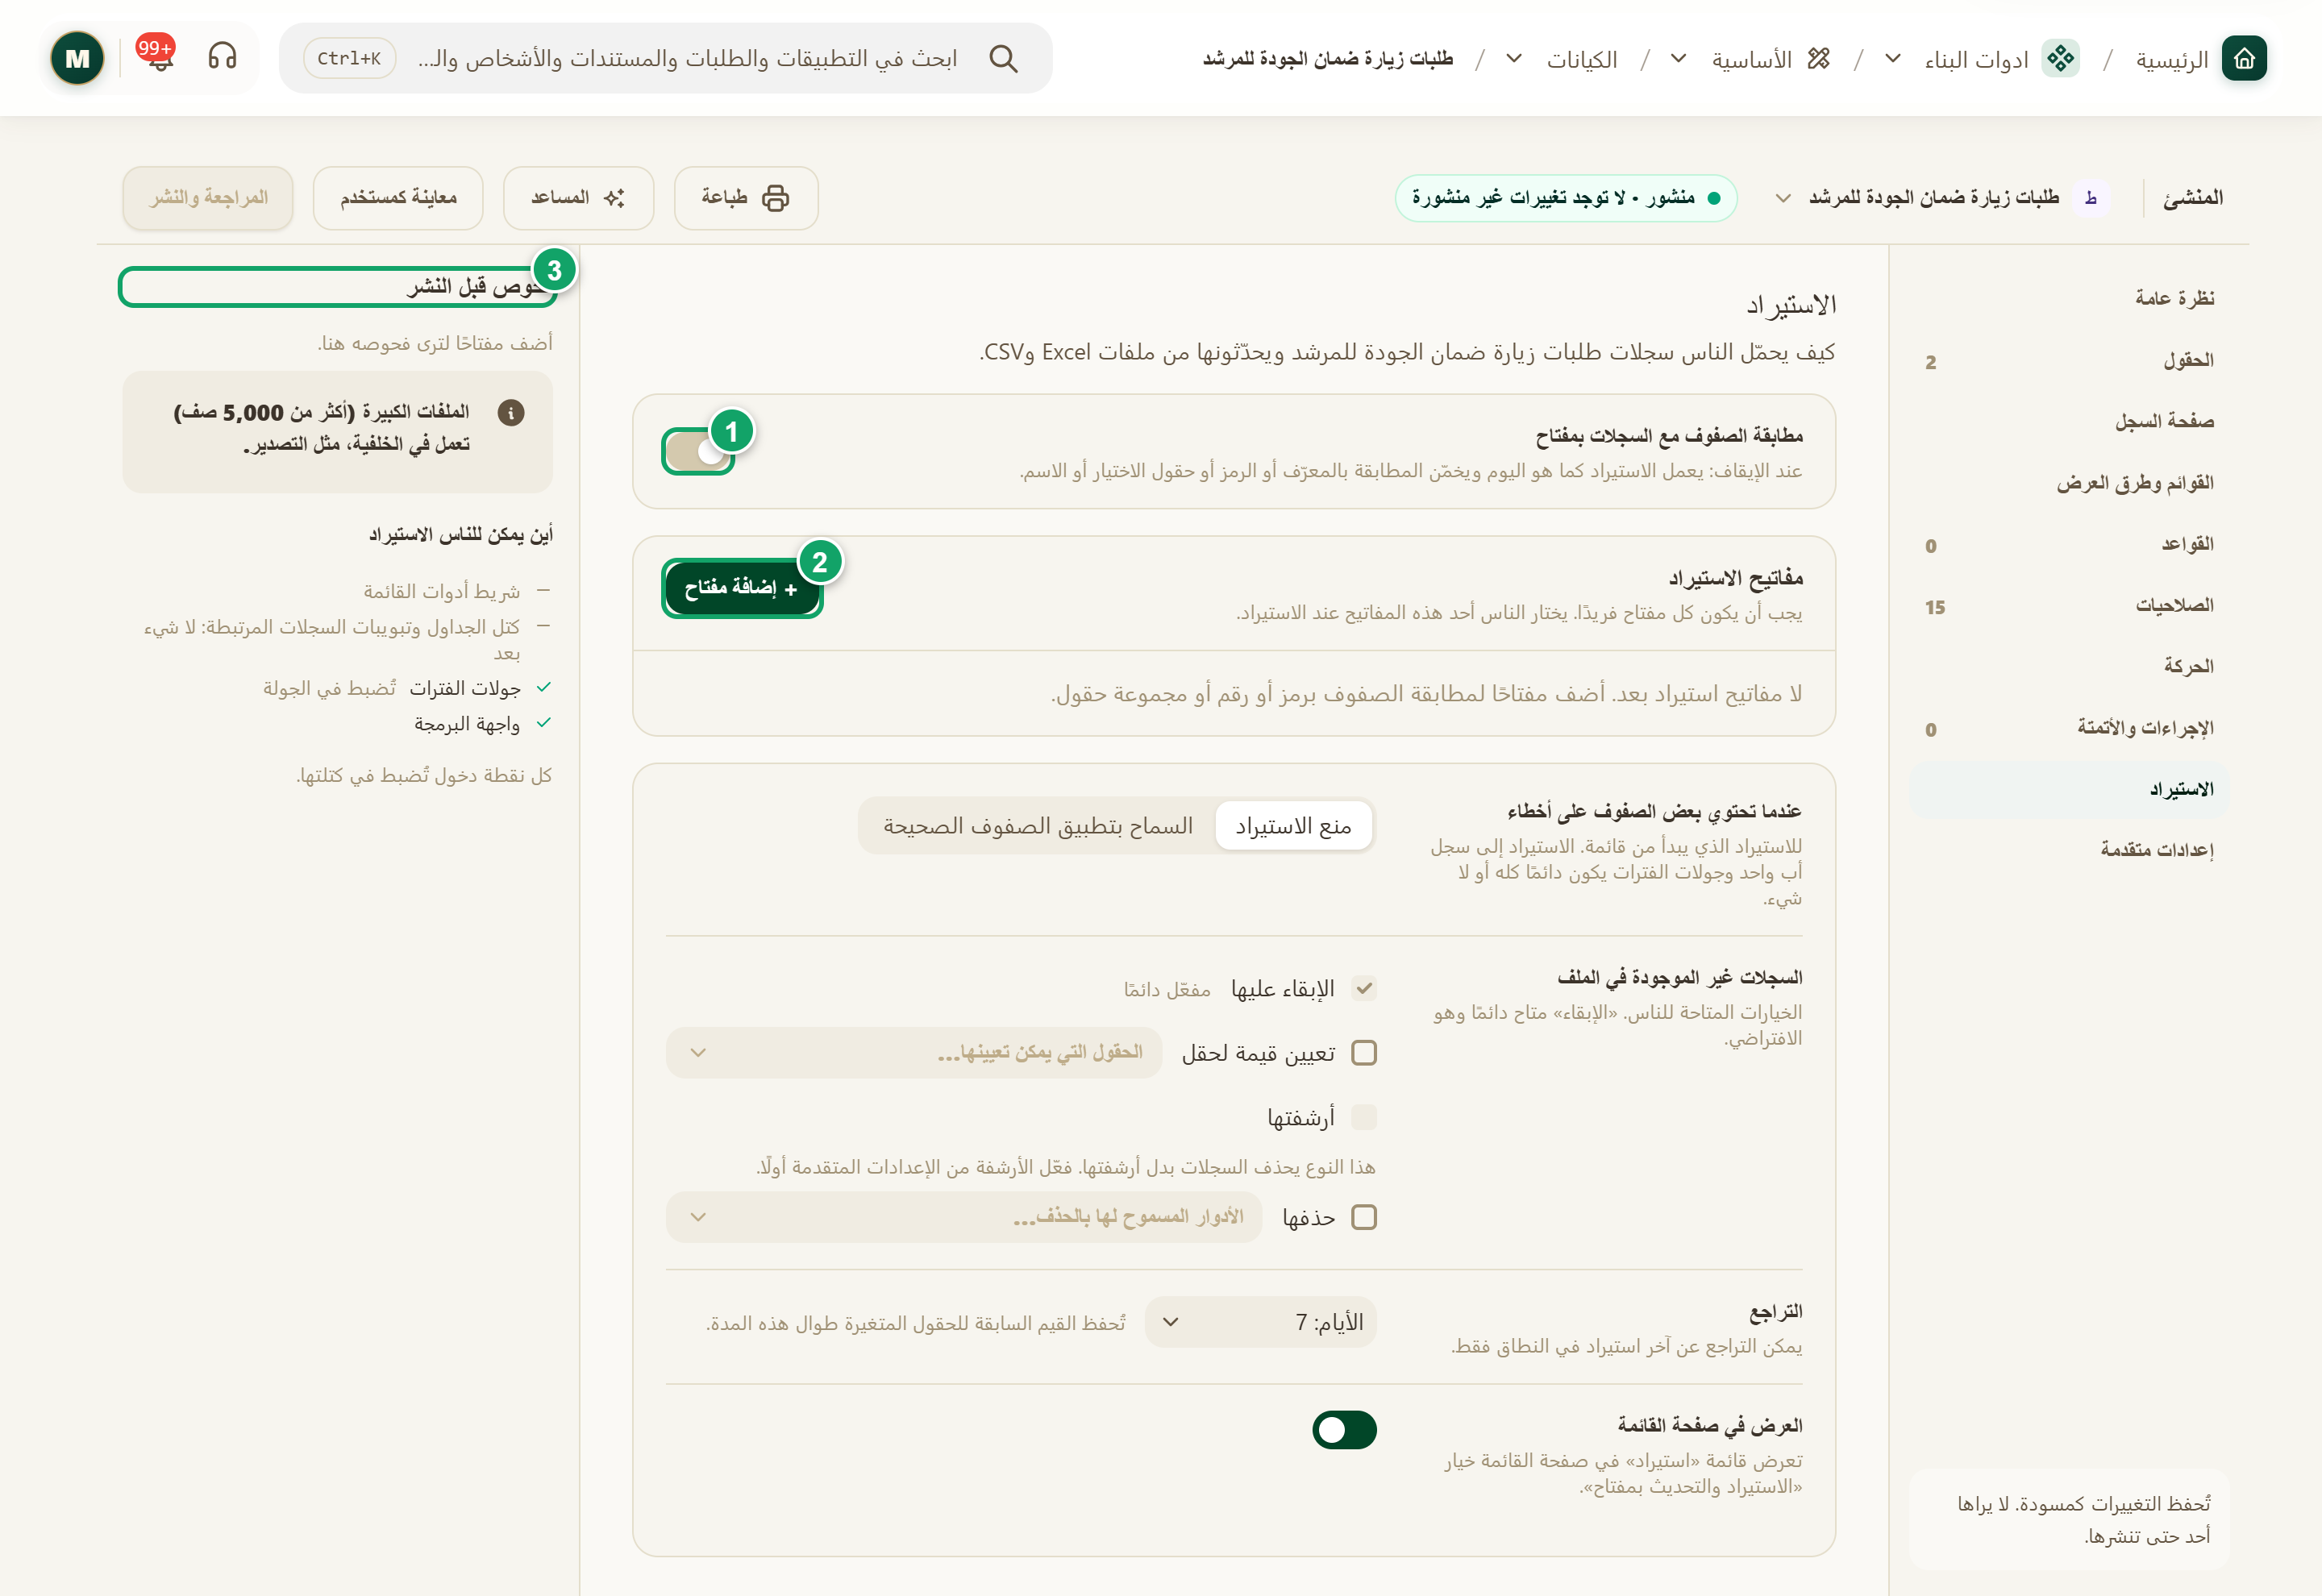
\includegraphics[width=0.95\linewidth,height=0.72\textheight,keepaspectratio]{figures/screens/ch06-ws-import-ar.png}
\caption{قسم «الاستيراد»}
\label{fig:builder-import-screen}
\shotnote{يحدد القسم طريقة تحديث السجلات من ملفات Excel وCSV، والمطابقة بالمفاتيح متوقفة هنا. ① مفتاح «مطابقة الصفوف مع السجلات بمفتاح». ② «+ إضافة مفتاح»: يضيف الحقل الذي تُطابق به الصفوف. ③ «فحوص قبل النشر»: تظهر فيها نتيجة «تشغيل الفحص» بعد إضافة مفتاح، لتتأكد من أنه فريد في السجلات المحفوظة.}
\end{figure}


\begin{table}[H]
\centering
\caption{ما الذي تجده هنا؟}
\label{tab:builder-import-data}
\begin{tabularx}{\linewidth}{R{3.6cm} Y}
\rcHeaderRow
\thh{الجزء} & \thh{المحتوى والإجراء}\\
مطابقة الصفوف مع السجلات بمفتاح & يفعّل الاستيراد بالمفاتيح. وعند الإيقاف يخمّن الاستيراد المطابقة كما في السابق.\\
مفاتيح الاستيراد & لكل مفتاح الحقول التي «يتكوّن من»ها، وأين يكون «فريد ضمن»ه، وطريقة «التوحيد» مثل تجاهل المسافات أو الأصفار البادئة، وهل هو «مدعوم بـ» قيمة فريدة، وحالته «جاهز» أو «مشكلة».\\
السلوك & ما يحدث «عندما تحتوي بعض الصفوف على أخطاء»: «منع الاستيراد» أو «السماح بتطبيق الصفوف الصحيحة»، وما يحدث لـ«السجلات غير الموجودة في الملف»: الإبقاء عليها أو أرشفتها أو حذفها، ومدة «التراجع» عن آخر استيراد.\\
فحوص قبل النشر & «تشغيل الفحص» يتأكد من أن المفتاح فريد في السجلات المحفوظة، ويعرض السجلات المتكررة أو الفارغة.\\
\end{tabularx}
\end{table}

\begin{figure}[H]
\centering
\begin{tikzpicture}[node distance=0.5cm]
\node[stepBox] (a) {\RL{إضافة مفتاح استيراد}};
\node[stepBox,below=of a] (b) {\RL{تشغيل الفحص}};
\node[stepBox,below=of b] (c) {\RL{ضبط السلوك}};
\node[stepBox,below=of c] (d) {\RL{النشر ثم استيراد ملف}};
\draw[flowsTo] (a) -- (b);
\draw[flowsTo] (b) -- (c);
\draw[flowsTo] (c) -- (d);
\end{tikzpicture}
\rclegend
\caption{تجهيز الاستيراد بالمفاتيح}
\label{fig:builder-import-flow}
\shotnote{يضع المخطط الفحص بعد إضافة المفتاح مباشرة، لأن المفتاح الذي تتكرر قيمته بين سجلين لا يعرف أيهما يحدّث. ثم تحدد ما يحدث للأخطاء والسجلات الغائبة عن الملف، لأن الاختيار الخاطئ هنا قد يؤرشف سجلات أو يحذفها. ولا يعمل شيء من ذلك قبل النشر.}
\end{figure}

\subsection{خطوات العمل والتحقق}
\begin{enumerate}
\item افتح نوع السجلات واختر «الاستيراد»، ثم فعّل «مطابقة الصفوف مع السجلات بمفتاح».
\item اضغط «+ إضافة مفتاح»، واختر الحقل الذي يميّز كل سجل، مثل الرمز أو الرقم التسلسلي.
\item اضغط «تشغيل الفحص»، وعالج أي سجلات متكررة أو فارغة يظهرها.
\item اختر السلوك المناسب للأخطاء والسجلات الغائبة، ثم انشر التغييرات.
\end{enumerate}

\textbf{تحقق ومعالجة المشكلة:} يجب أن تظهر حالة المفتاح «جاهز» وأن يظهر في الفحص أنه فريد. فإذا ظهر أن بعض السجلات ستتشارك المفتاح نفسه، فصحّح قيمها أولاً. ولا تختر حذف السجلات الغائبة عن الملف إلا عن قصد، واستخدم «التراجع» إذا أخطأ استيراد.

\clearpage
\section{إعدادات متقدمة}
\label{sec:builder-feature-advanced}

تضم «إعدادات متقدمة» إعدادات نادراً ما تتغير بعد البداية، مثل اسم السجل في القوائم، ومنع التكرار، والتسلسل بين السجلات، والتطبيق الذي يظهر فيه النوع. وهي جزء من المسودة مثل بقية الأقسام، فلا تصل إلى الفريق قبل النشر.

\textbf{المسار ومن يستخدمه:} نوع السجلات ← «إعدادات متقدمة». يستخدمه من يبني النوع، غالباً عند إنشائه ثم عند الحاجة فقط.

\begin{rcnote}[مثال: شركة الأفق]
يجعل مسؤول النظام «اسم السجل» في طلبات الزيارة هو الرقم التسلسلي مع اسم الفرع، ويضع النوع في تطبيق «خدمات الفروع»، ويختار «أرشفة السجلات بدل حذفها» حتى لا يضيع أي طلب. وتطابق اختياراته الرقمين ① و④.
\end{rcnote}

\begin{figure}[H]
\centering
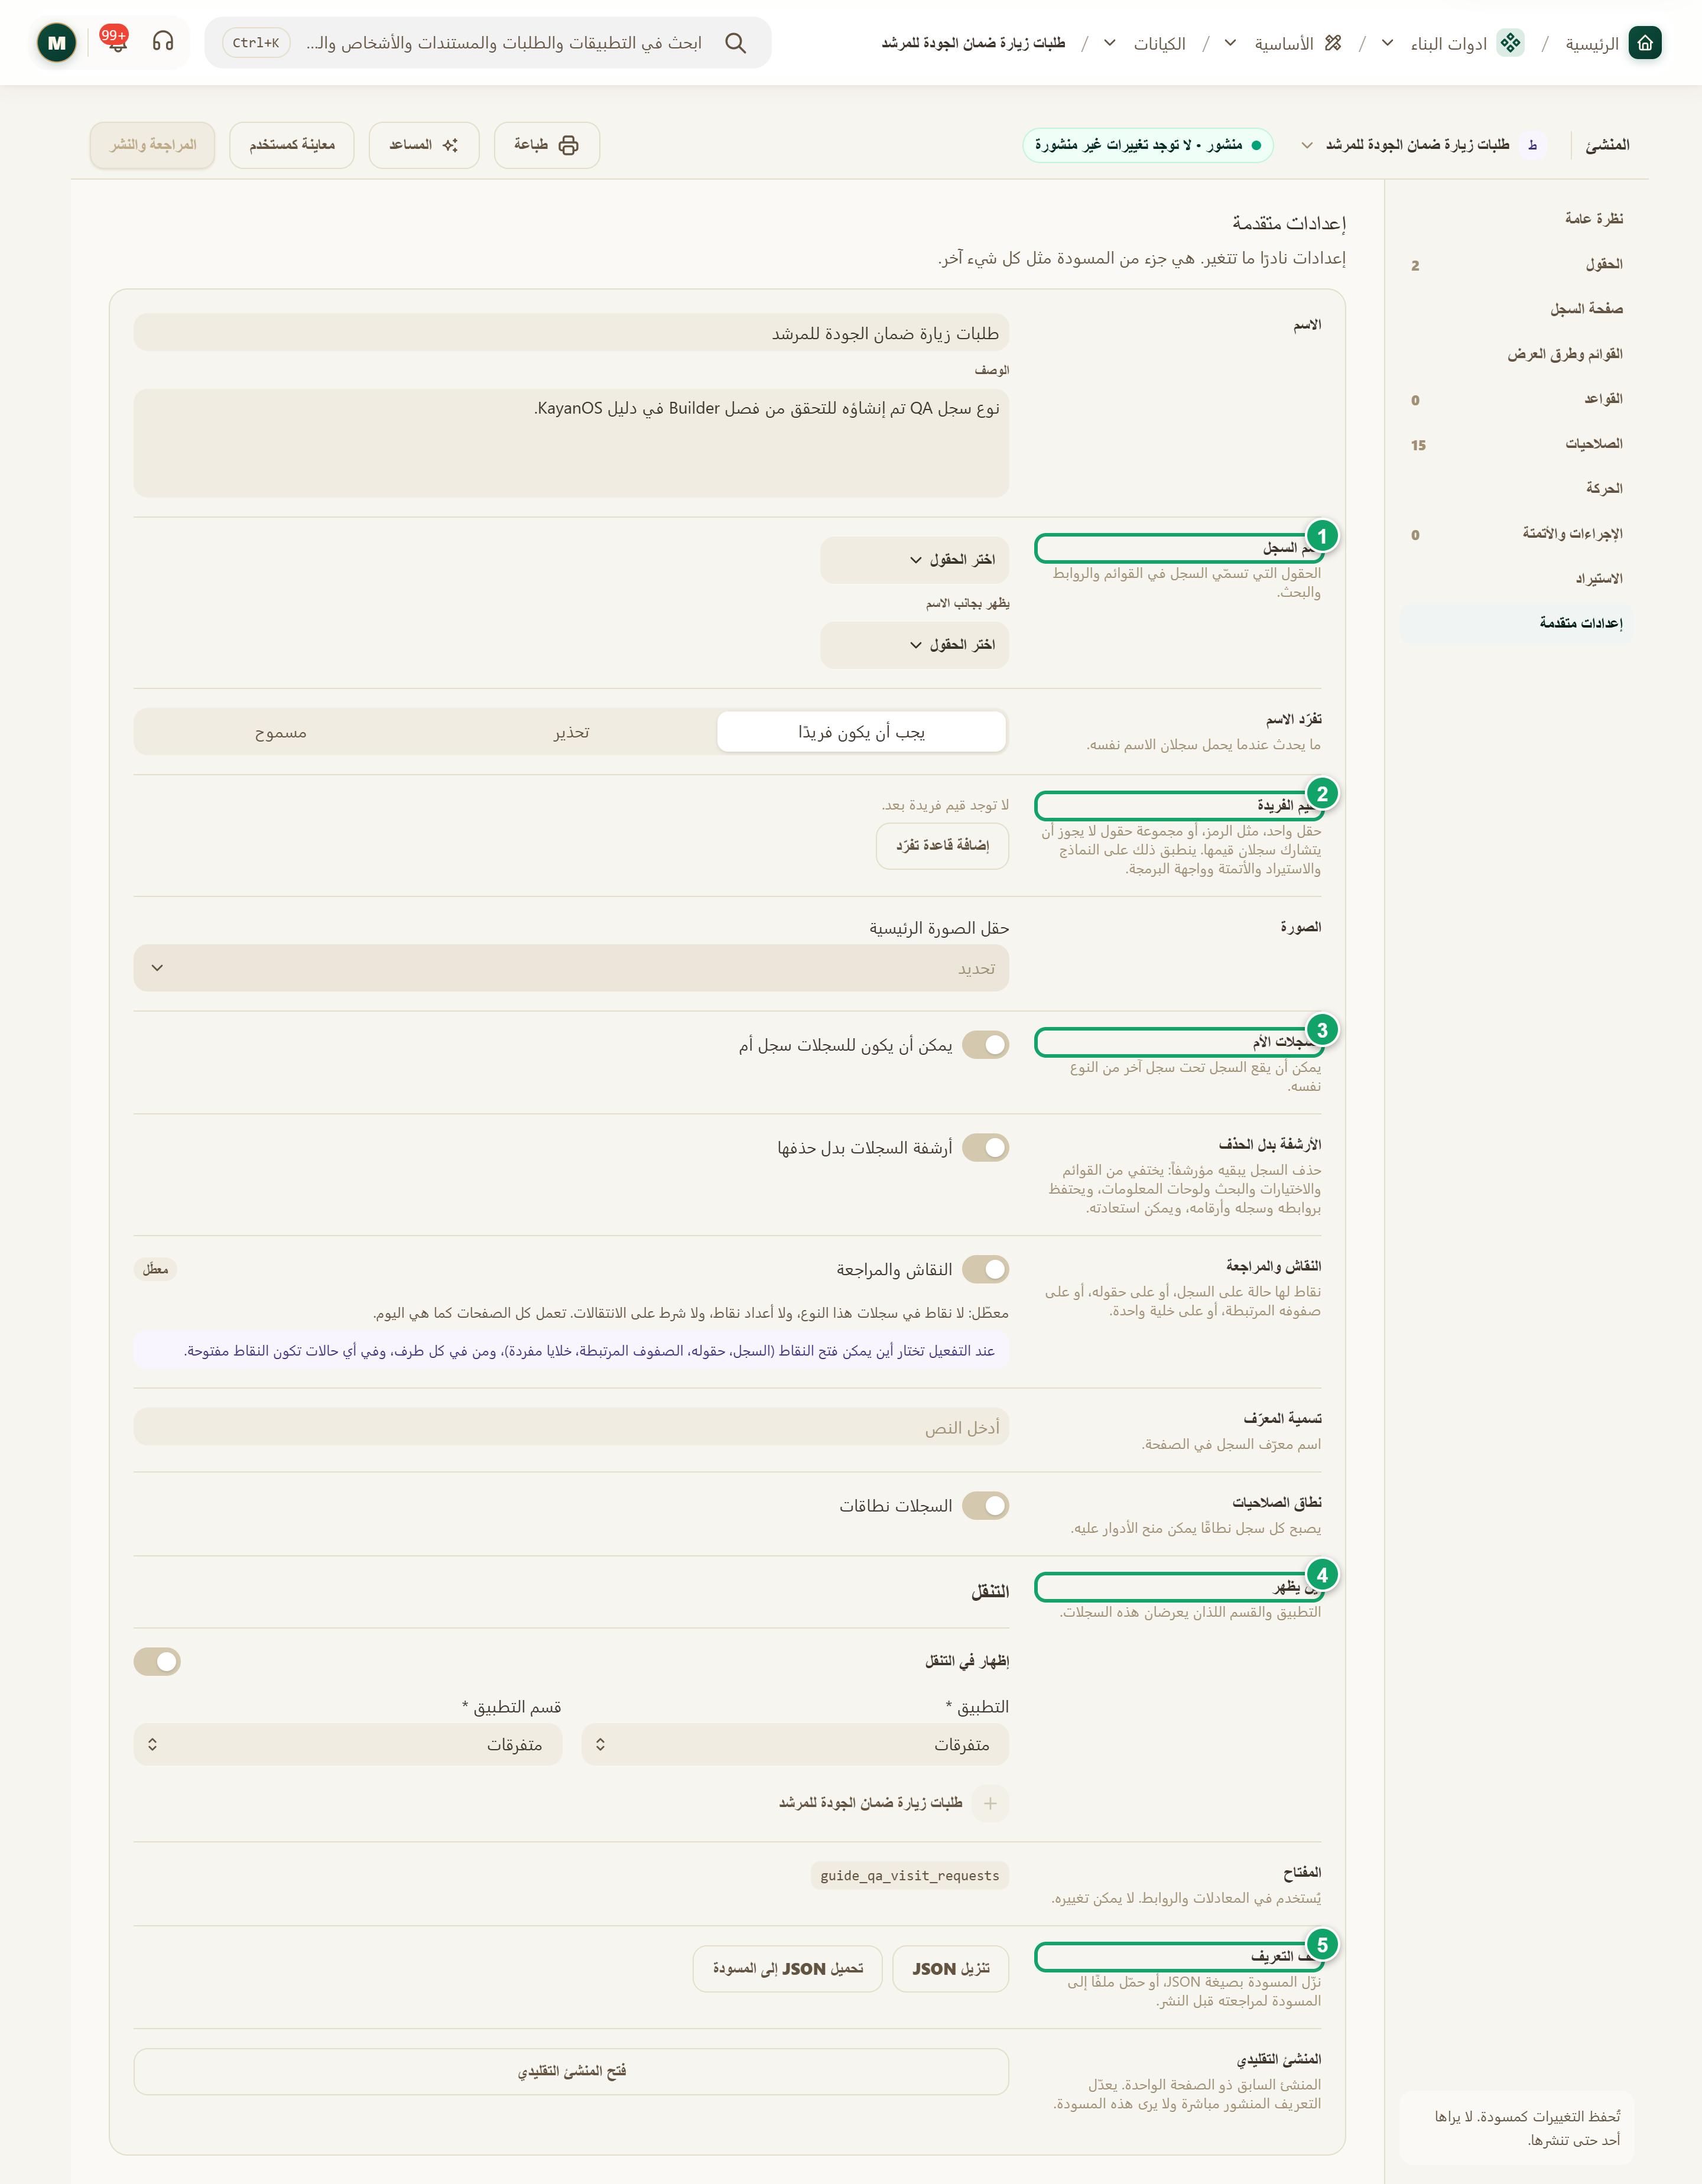
\includegraphics[width=0.95\linewidth,height=0.72\textheight,keepaspectratio]{figures/screens/ch06-ws-advanced-ar.png}
\caption{قسم «إعدادات متقدمة»}
\label{fig:builder-advanced-screen}
\shotnote{يجمع القسم إعدادات نادراً ما تتغير، ويظهر هنا لنوع السجلات الاختباري. ① «اسم السجل»: الحقول التي تسمّي السجل. ② «القيم الفريدة»: تمنع تكرار رمز أو مجموعة قيم. ③ «السجلات الأم»: تسمح بتسلسل أب وأبناء. ④ «أين يظهر»: التطبيق والقسم. ⑤ «ملف التعريف»: تنزيل الإعداد أو تحميله بصيغة JSON.}
\end{figure}


\begin{table}[H]
\centering
\caption{ما الذي تجده هنا؟}
\label{tab:builder-advanced-data}
\begin{tabularx}{\linewidth}{R{3.6cm} Y}
\rcHeaderRow
\thh{الإعداد} & \thh{المعنى}\\
اسم السجل & الحقول التي تسمّي السجل في القوائم والروابط والبحث، وحقل اختياري «يظهر بجانب الاسم».\\
تفرّد الاسم & ما يحدث عندما يحمل سجلان الاسم نفسه: «يجب أن يكون فريدًا» أو «تحذير» أو «مسموح».\\
القيم الفريدة & حقل، مثل الرمز، أو مجموعة حقول لا يجوز أن يتشارك سجلان قيمها، في النماذج والاستيراد والأتمتة أيضاً.\\
الصورة & الحقل الذي يُستخدم صورةً رئيسية للسجل.\\
السجلات الأم & تسمح بأن يقع السجل تحت سجل آخر من النوع نفسه، فتظهر طريقة العرض «شجرة».\\
الأرشفة بدل الحذف & يبقى السجل المحذوف مؤرشفاً: يختفي من القوائم والبحث، ويحتفظ بروابطه وأرقامه، ويمكن استعادته. ويمكنك أن تؤرشف معه سجلاته الفرعية والمهام المرتبطة به.\\
النقاش والمراجعة & يسمح بفتح نقاط لها حالة على السجل أو حقوله أو صفوفه المرتبطة أو خلية واحدة، فتظهر في تبويب «النقاط» في صفحة السجل. ويبقى متوقفاً حتى تشغّله.\\
تسمية المعرّف & اسم معرّف السجل في الصفحة.\\
نطاق الصلاحيات & يجعل كل سجل نطاقاً يمكن منح الأدوار عليه، مثل منح مدير فرع صلاحية على فرعه فقط.\\
أين يظهر & «التطبيق» و«قسم التطبيق» اللذان يعرضان السجلات، و«إظهار في التنقل»، والأيقونة.\\
المفتاح & يُستخدم في المعادلات والروابط، ولا يمكن تغييره.\\
ملف التعريف & «تنزيل JSON» لنسخة من المسودة، أو «تحميل JSON إلى المسودة» لمراجعته قبل النشر.\\
المنشئ التقليدي & المنشئ السابق ذو الصفحة الواحدة؛ يعدّل التعريف المنشور مباشرة ولا يرى المسودة، فاستخدمه بحذر.\\
\end{tabularx}
\end{table}

\begin{figure}[H]
\centering
\begin{tikzpicture}[node distance=0.5cm]
\node[entity] (adv) {\RL{إعدادات متقدمة}};
\node[entityOpt,below right=0.7cm and 0.3cm of adv] (tree) {\RL{السجلات الأم}};
\node[entityOpt,below left=0.7cm and 0.3cm of adv] (scope) {\RL{نطاق الصلاحيات}};
\node[entityOpt,below=0.7cm of tree] (treeview) {\RL{عرض الشجرة}};
\node[entityOpt,below=0.7cm of scope] (roles) {\RL{أدوار على سجل واحد}};
\draw[dependsOnOpt] (adv.south) -- ++(0,-0.3) -| (tree.north);
\draw[dependsOnOpt] (adv.south) -- ++(0,-0.3) -| (scope.north);
\draw[dependsOnOpt] (tree) -- (treeview);
\draw[dependsOnOpt] (scope) -- (roles);
\end{tikzpicture}
\rclegend
\caption{إعدادان يفتحان إمكانات أخرى}
\label{fig:builder-advanced-effects}
\shotnote{يوضّح الشكل أن بعض الإعدادات المتقدمة شرط لإمكانات في أقسام أخرى: فتفعيل «السجلات الأم» يتيح عرض «شجرة» في القوائم، وتفعيل «نطاق الصلاحيات» يتيح منح أدوار على سجل واحد. لذلك إذا لم تجد إحدى هذه الإمكانات، فابدأ بمراجعة هذا القسم.}
\end{figure}

\subsection{خطوات العمل والتحقق}
\begin{enumerate}
\item افتح نوع السجلات واختر «إعدادات متقدمة».
\item اختر «اسم السجل» من حقول تميّز السجل فعلاً، مثل الرقم التسلسلي.
\item أضف «قاعدة تفرّد» للحقول التي يجب ألا تتكرر، وراجع التحذير إن وُجدت تكرارات حالية.
\item راجع «أين يظهر» لتتأكد من التطبيق والقسم، ثم انشر التغييرات.
\end{enumerate}

\textbf{تحقق ومعالجة المشكلة:} بعد النشر يجب أن تظهر السجلات في القوائم والبحث بالاسم الذي اخترته، وأن يُرفض إدخال قيمة فريدة مكررة. وقبل أي تعديل كبير، استخدم «تنزيل JSON» لتحتفظ بنسخة من الإعداد.

\clearpage
\section{المراجعة والنشر}
\label{sec:builder-feature-publish}

يحفظ «المنشئ» كل تعديل تجريه مسودةً، ولا يرى أحد غيرك هذه التغييرات حتى تنشرها. وتعرض «المراجعة والنشر» التغييرات كلها قبل النشر، وتمنعه إذا بقيت مشكلة يجب حلها. وكل نشر يُنشئ إصداراً جديداً يمكنك الرجوع إليه لاحقاً.

\textbf{المسار ومن يستخدمه:} نوع السجلات ← «المراجعة والنشر». يستخدمه من يبني النوع بعد أن ينهي مجموعة من التعديلات.

\begin{rcnote}[مثال: شركة الأفق]
قبل إطلاق «طلبات الزيارة» يستخدم مسؤول النظام «معاينة كمستخدم» ليرى الصفحة كما يراها عمر حداد، ثم ينشر الإصدار الأول، ويطلب من عمر تجربة طلب لزيارة فرع حلب. ويستخدم ③ قبل أن ينشر من ④.
\end{rcnote}

\begin{figure}[H]
\centering
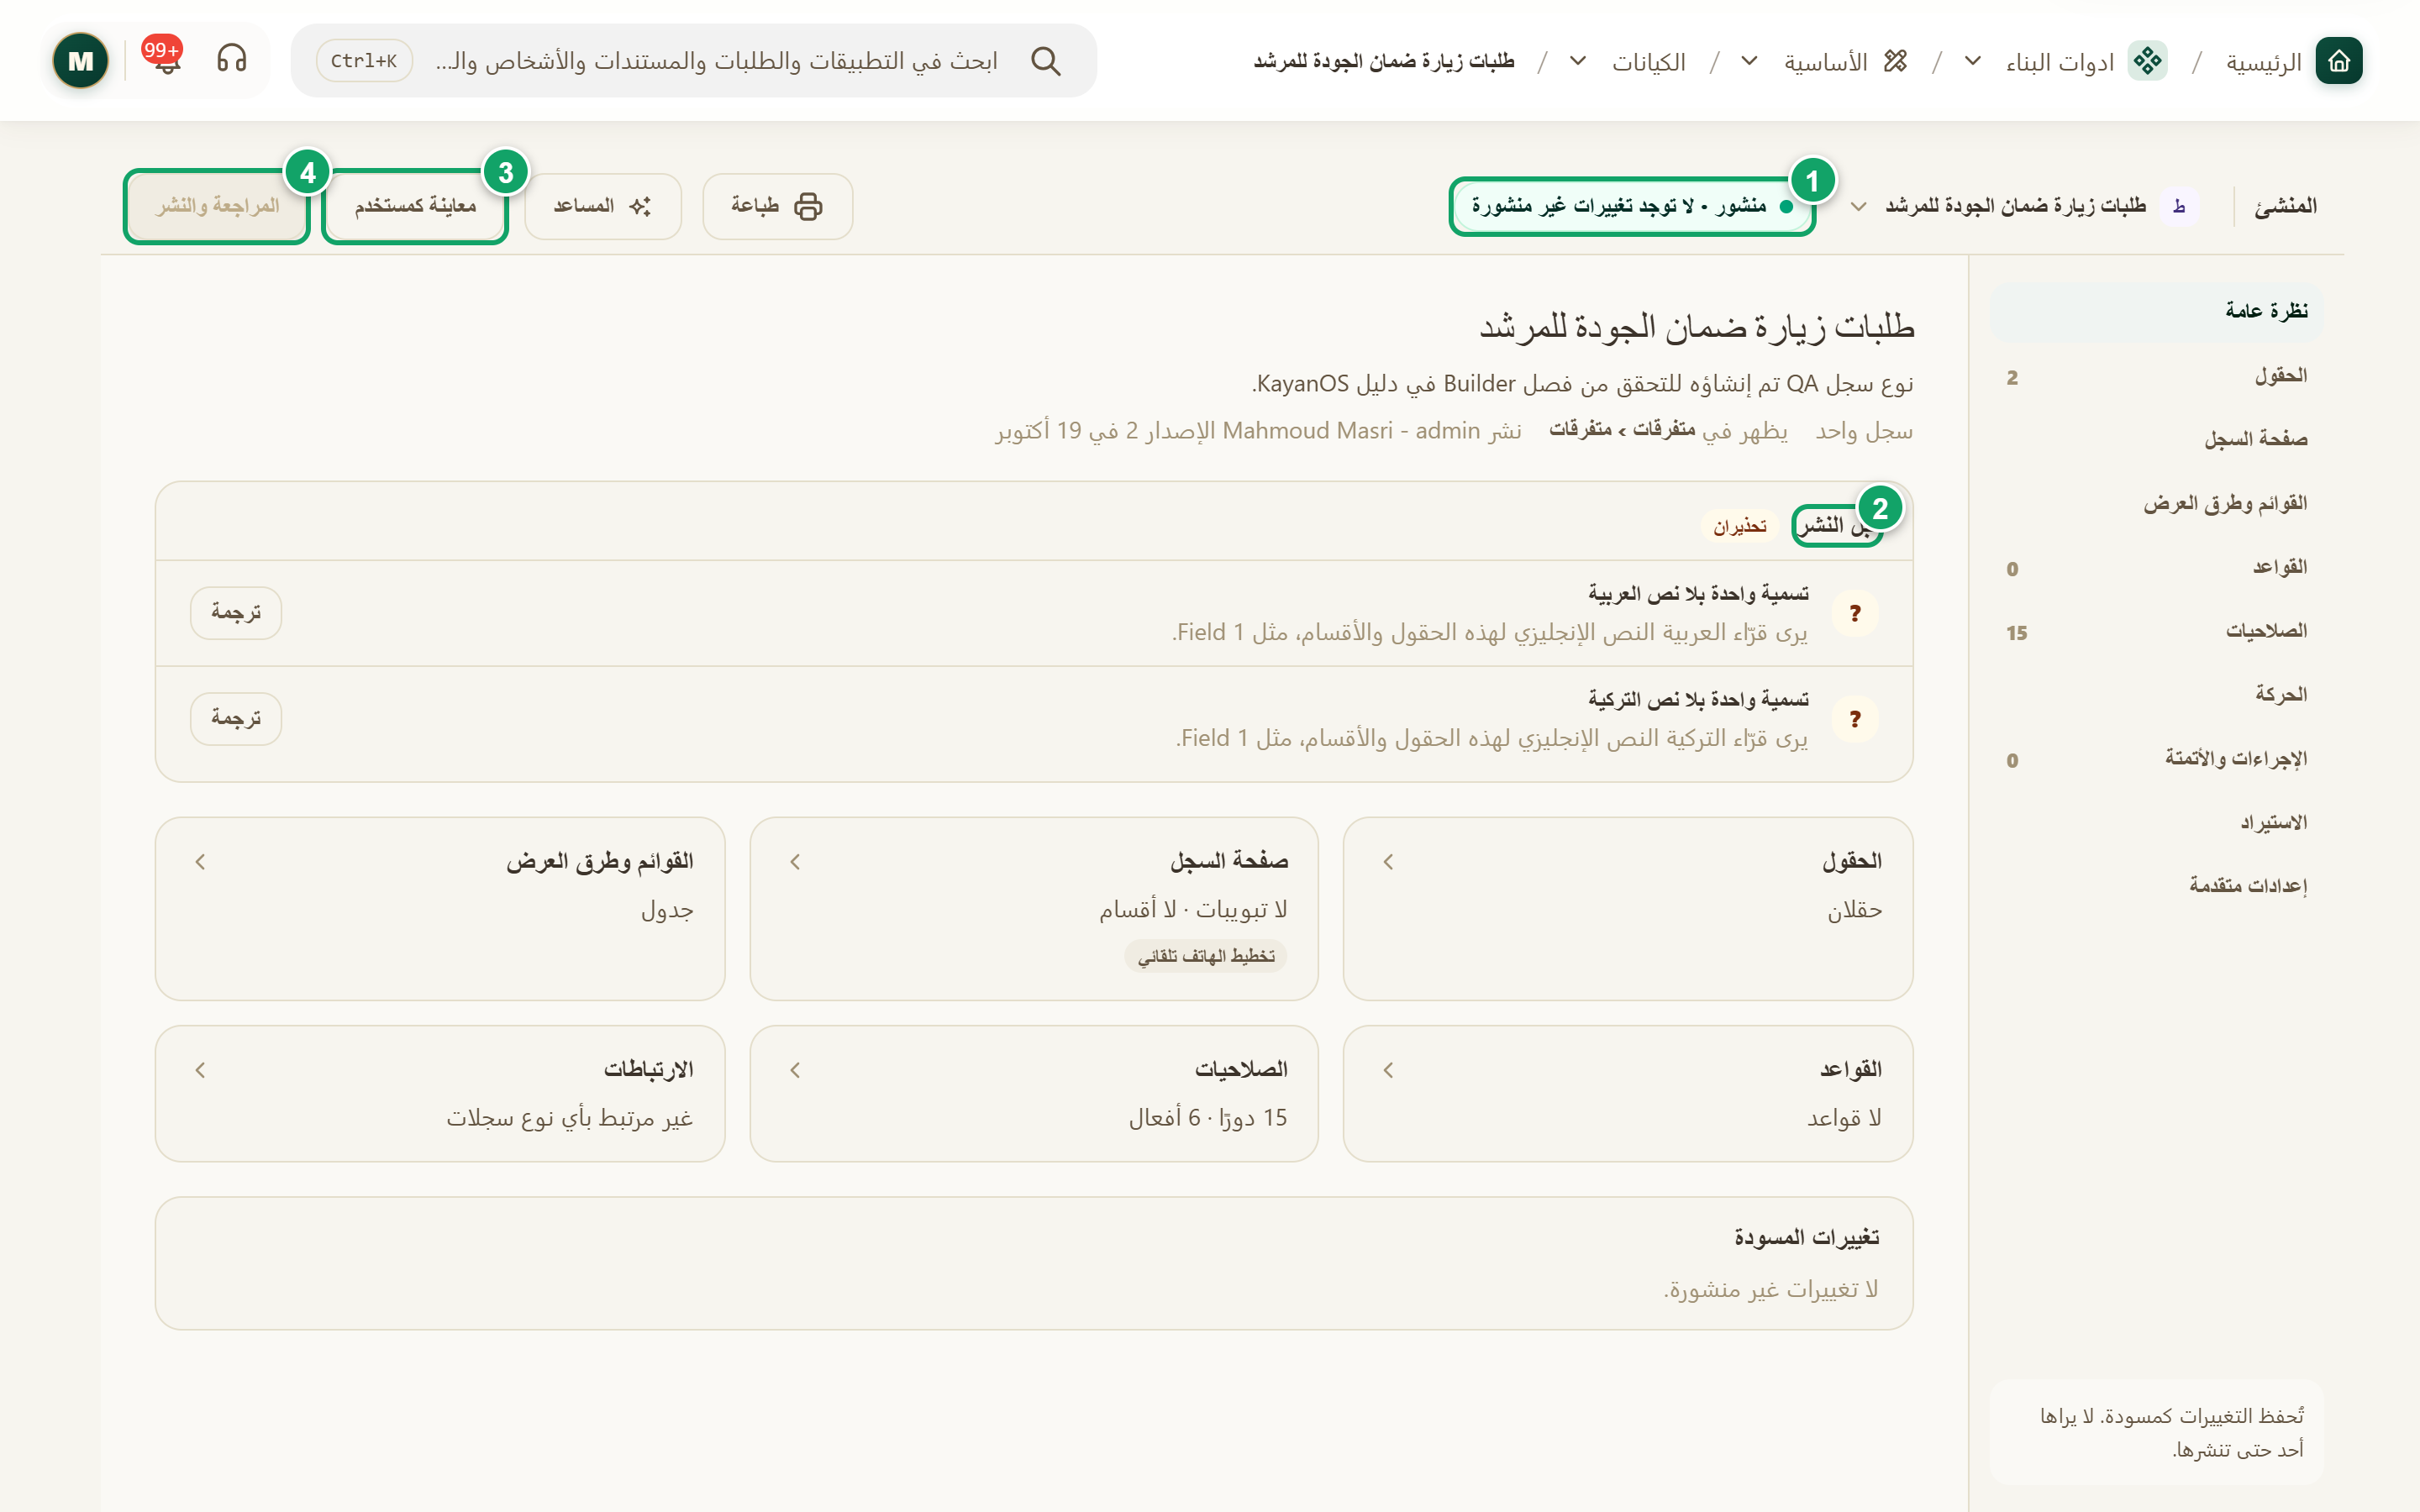
\includegraphics[width=0.95\linewidth,height=0.72\textheight,keepaspectratio]{figures/screens/ch06-ws-overview-ar.png}
\caption{«نظرة عامة» بعد النشر}
\label{fig:builder-publish-screen}
\shotnote{تلخّص «نظرة عامة» حالة النوع وما يجب إصلاحه قبل النشر. والنوع الاختباري هنا منشور في الإصدار 2 بعد اختبار هذا الفصل، وتبقى تحذيرات ترجمة لا تمنع النشر. ① الحالة: «منشور · لا توجد تغييرات غير منشورة». ② «قبل النشر»: المشكلات والتحذيرات. ③ «معاينة كمستخدم». ④ «المراجعة والنشر»: يفتح قائمة التغييرات وزر النشر.}
\end{figure}


\begin{table}[H]
\centering
\caption{ما الذي تجده هنا؟}
\label{tab:builder-publish-data}
\begin{tabularx}{\linewidth}{R{3.6cm} Y}
\rcHeaderRow
\thh{العنصر} & \thh{المعنى والإجراء}\\
مسودة & حالة النوع وفيه تغييرات لم تُنشر. أما «منشور · لا توجد تغييرات غير منشورة» فيعني أن ما يراه الفريق هو آخر ما بنيته.\\
نظرة عامة & ملخص الحقول والصفحة والقوائم والقواعد، و«قبل النشر» تعرض المشكلات التي تمنع النشر والتحذيرات.\\
معاينة كمستخدم & تعرض النوع كما سيراه المستخدم قبل النشر.\\
المراجعة والنشر & تفتح نافذة «مراجعة التغييرات» التي تجمع التغييرات حسب القسم، ولكل تغيير خانة اختيار تستطيع إلغاءها فيبقى في المسودة. وتكتب وصفاً اختيارياً للإصدار، ثم تضغط «نشر N تغيير».\\
تغييرات معلّقة & إذا فعّلت المؤسسة اعتماد تغييرات أنواع السجلات، فلا تُطبَّق التغييرات التي تشملها سياسة الاعتماد عند النشر، بل تُحفظ «تغييرات معلّقة» ترسلها للاعتماد من الشريط أعلى المنشئ. ويبقى النوع وسجلاته يعملان بالتعريف الحالي حتى تُعتمد وتُطبَّق.\\
سجل الإصدارات & يعرض الإصدارات السابقة. و«استعادة» إصدار تضع حقوله وتخطيط صفحته في المسودة، ولا يصل شيء إلى الفريق حتى تنشر.\\
تجاهل المسودة & يزيل التغييرات غير المنشورة للجميع، ويبقى التعريف المنشور كما هو.\\
\end{tabularx}
\end{table}

\begin{figure}[H]
\centering
\begin{tikzpicture}[node distance=0.5cm]
\node[stepBox] (a) {\RL{تعديلات تُحفظ مسودة}};
\node[stepBox,below=of a] (b) {\RL{حل مشكلات «قبل النشر»}};
\node[stepBox,below=of b] (c) {\RL{معاينة كمستخدم}};
\node[stepBox,below=of c] (d) {\RL{النشر: إصدار جديد}};
\draw[flowsTo] (a) -- (b);
\draw[flowsTo] (b) -- (c);
\draw[flowsTo] (c) -- (d);
\end{tikzpicture}
\rclegend
\caption{من المسودة إلى الإصدار المنشور}
\label{fig:builder-publish-flow}
\shotnote{يبيّن المخطط أن النشر خطوة مقصودة يتخذها من يبني النوع، لا نتيجة تلقائية للحفظ. فالمسودة تجمع التعديلات بأمان، ولا يصل أي منها إلى الفريق قبل حل المشكلات والنشر، ويصبح كل نشر إصداراً يمكن استعادته.}
\end{figure}

\subsection{خطوات العمل والتحقق}
\begin{enumerate}
\item افتح «نظرة عامة» وراجع «قبل النشر»، ثم أصلح كل مشكلة تمنع النشر.
\item اضغط «معاينة كمستخدم» وراجع الصفحة والقوائم كما سيراها الفريق.
\item اضغط «المراجعة والنشر»، وراجع قائمة التغييرات، وألغِ اختيار أي تغيير تريد إبقاءه في المسودة، ثم اضغط «نشر N تغيير».
\item أنشئ سجلاً تجريبياً من قائمة النوع، ثم أعد فتحه وتأكد من حفظ قيمه.
\end{enumerate}

\textbf{تحقق ومعالجة المشكلة:} يجب أن تظهر رسالة بأن النوع «نُشر كإصدار» برقمه، وأن تتغير الحالة إلى «منشور · لا توجد تغييرات غير منشورة». فإذا ظهرت مشكلة بعد النشر، فافتح «سجل الإصدارات» واستعد الإصدار السابق إلى المسودة، ثم صحّحها وانشرها من جديد، لأن الاستعادة وحدها لا تغيّر ما يراه الفريق.


\chapter{التطبيقات والتنقل}
\label{ch:builder-navigation}

\section{ماذا ستضبط في هذا الفصل؟}
\label{sec:builder-navigation-intro}

لا يكفي أن تنشر نوع السجلات حتى يستخدمه الفريق؛ فيجب أن يجده الأعضاء في المكان الذي يتوقعونه. ويشرح هذا الفصل صفحتين: «التطبيقات والتنقل» التي ترتّب التطبيقات وأقسامها في القائمة وتُظهرها أو تخفيها، و«التنقل حسب العمل» التي تحدد ما يراه كل عضو أولاً عند دخوله.

\begin{rcnote}[مثال: شركة الأفق]
بعد نشر «طلبات الزيارة» يضيف مسؤول النظام تطبيق «خدمات الفروع»، ويضع فيه قسماً يعرض الطلبات، فيجده عمر حداد في القائمة دون أن يبحث عنه.
\end{rcnote}

\section{صفحات هذا الفصل}
\label{sec:builder-navigation-pages}

الصفحتان مستقلتان في قسم «الأساسية» من أدوات البناء. ابدأ بالأولى لترتيب القائمة، ثم استخدم الثانية عندما تريد تجربة أوضح لكل دور.

\begin{table}[H]
\centering
\caption{إظهار العمل للفريق}
\label{tab:builder-pages-navigation}
\rcZebra
\begin{tabularx}{\linewidth}{R{4.2cm} Y}
\rcHeaderRow
\thh{الصفحة وقسمها} & \thh{ماذا تقدم هذه الصفحة؟}\\
التطبيقات والتنقل — الأساسية & ترتّب التطبيقات والأقسام التي يراها الأعضاء، وتُظهرها أو تخفيها.\\
التنقل حسب العمل — الأساسية & تحدد ما يراه كل عضو أولاً: صفحة «مكتبي» وقائمة المستحق عليه والسياق المشترك.\\
\end{tabularx}
\end{table}

\clearpage
\section{التطبيقات والتنقل}
\label{sec:builder-feature-navigation}

تحدد صفحة «التطبيقات والتنقل» ما يراه الأعضاء في قائمة التطبيقات وترتيبه. وتعرض التنقل شجرةً من ثلاثة مستويات: التطبيق، ثم أقسامه، ثم الوحدات داخل كل قسم. والوحدة هي أي عنصر يفتحه العضو من القائمة: نوع سجلات أو نموذج أو لوحة معلومات أو صفحة أو صفحة مضمّنة في النظام.

ومن هذه الصفحة تعيد ترتيب العناصر بالسحب، وتُظهرها أو تخفيها بمفاتيح التشغيل. ولا تصل هذه التعديلات إلى الأعضاء فوراً، بل تبقى مسودة في الصفحة حتى تضغط «حفظ التغييرات»، فتستطيع أن تجرّب الترتيب وتتراجع عنه بأمان.

\textbf{المسار ومن يستخدمه:} «ادوات البناء» ← «الأساسية» ← «التطبيقات والتنقل». تظهر لمالك المؤسسة ومسؤولها فقط.

\begin{rcnote}[مثال: شركة الأفق]
يضيف مسؤول النظام تطبيق «خدمات الفروع» وقسماً فيه باسم «الزيارات»، ثم يسحب «طلبات الزيارة» إليه ويحفظ، فيجده عمر حداد في قائمة التطبيقات عند فتح الصفحة التالية. ويضيف التطبيق من ① ويحفظ من ⑤.
\end{rcnote}

\begin{figure}[H]
\centering
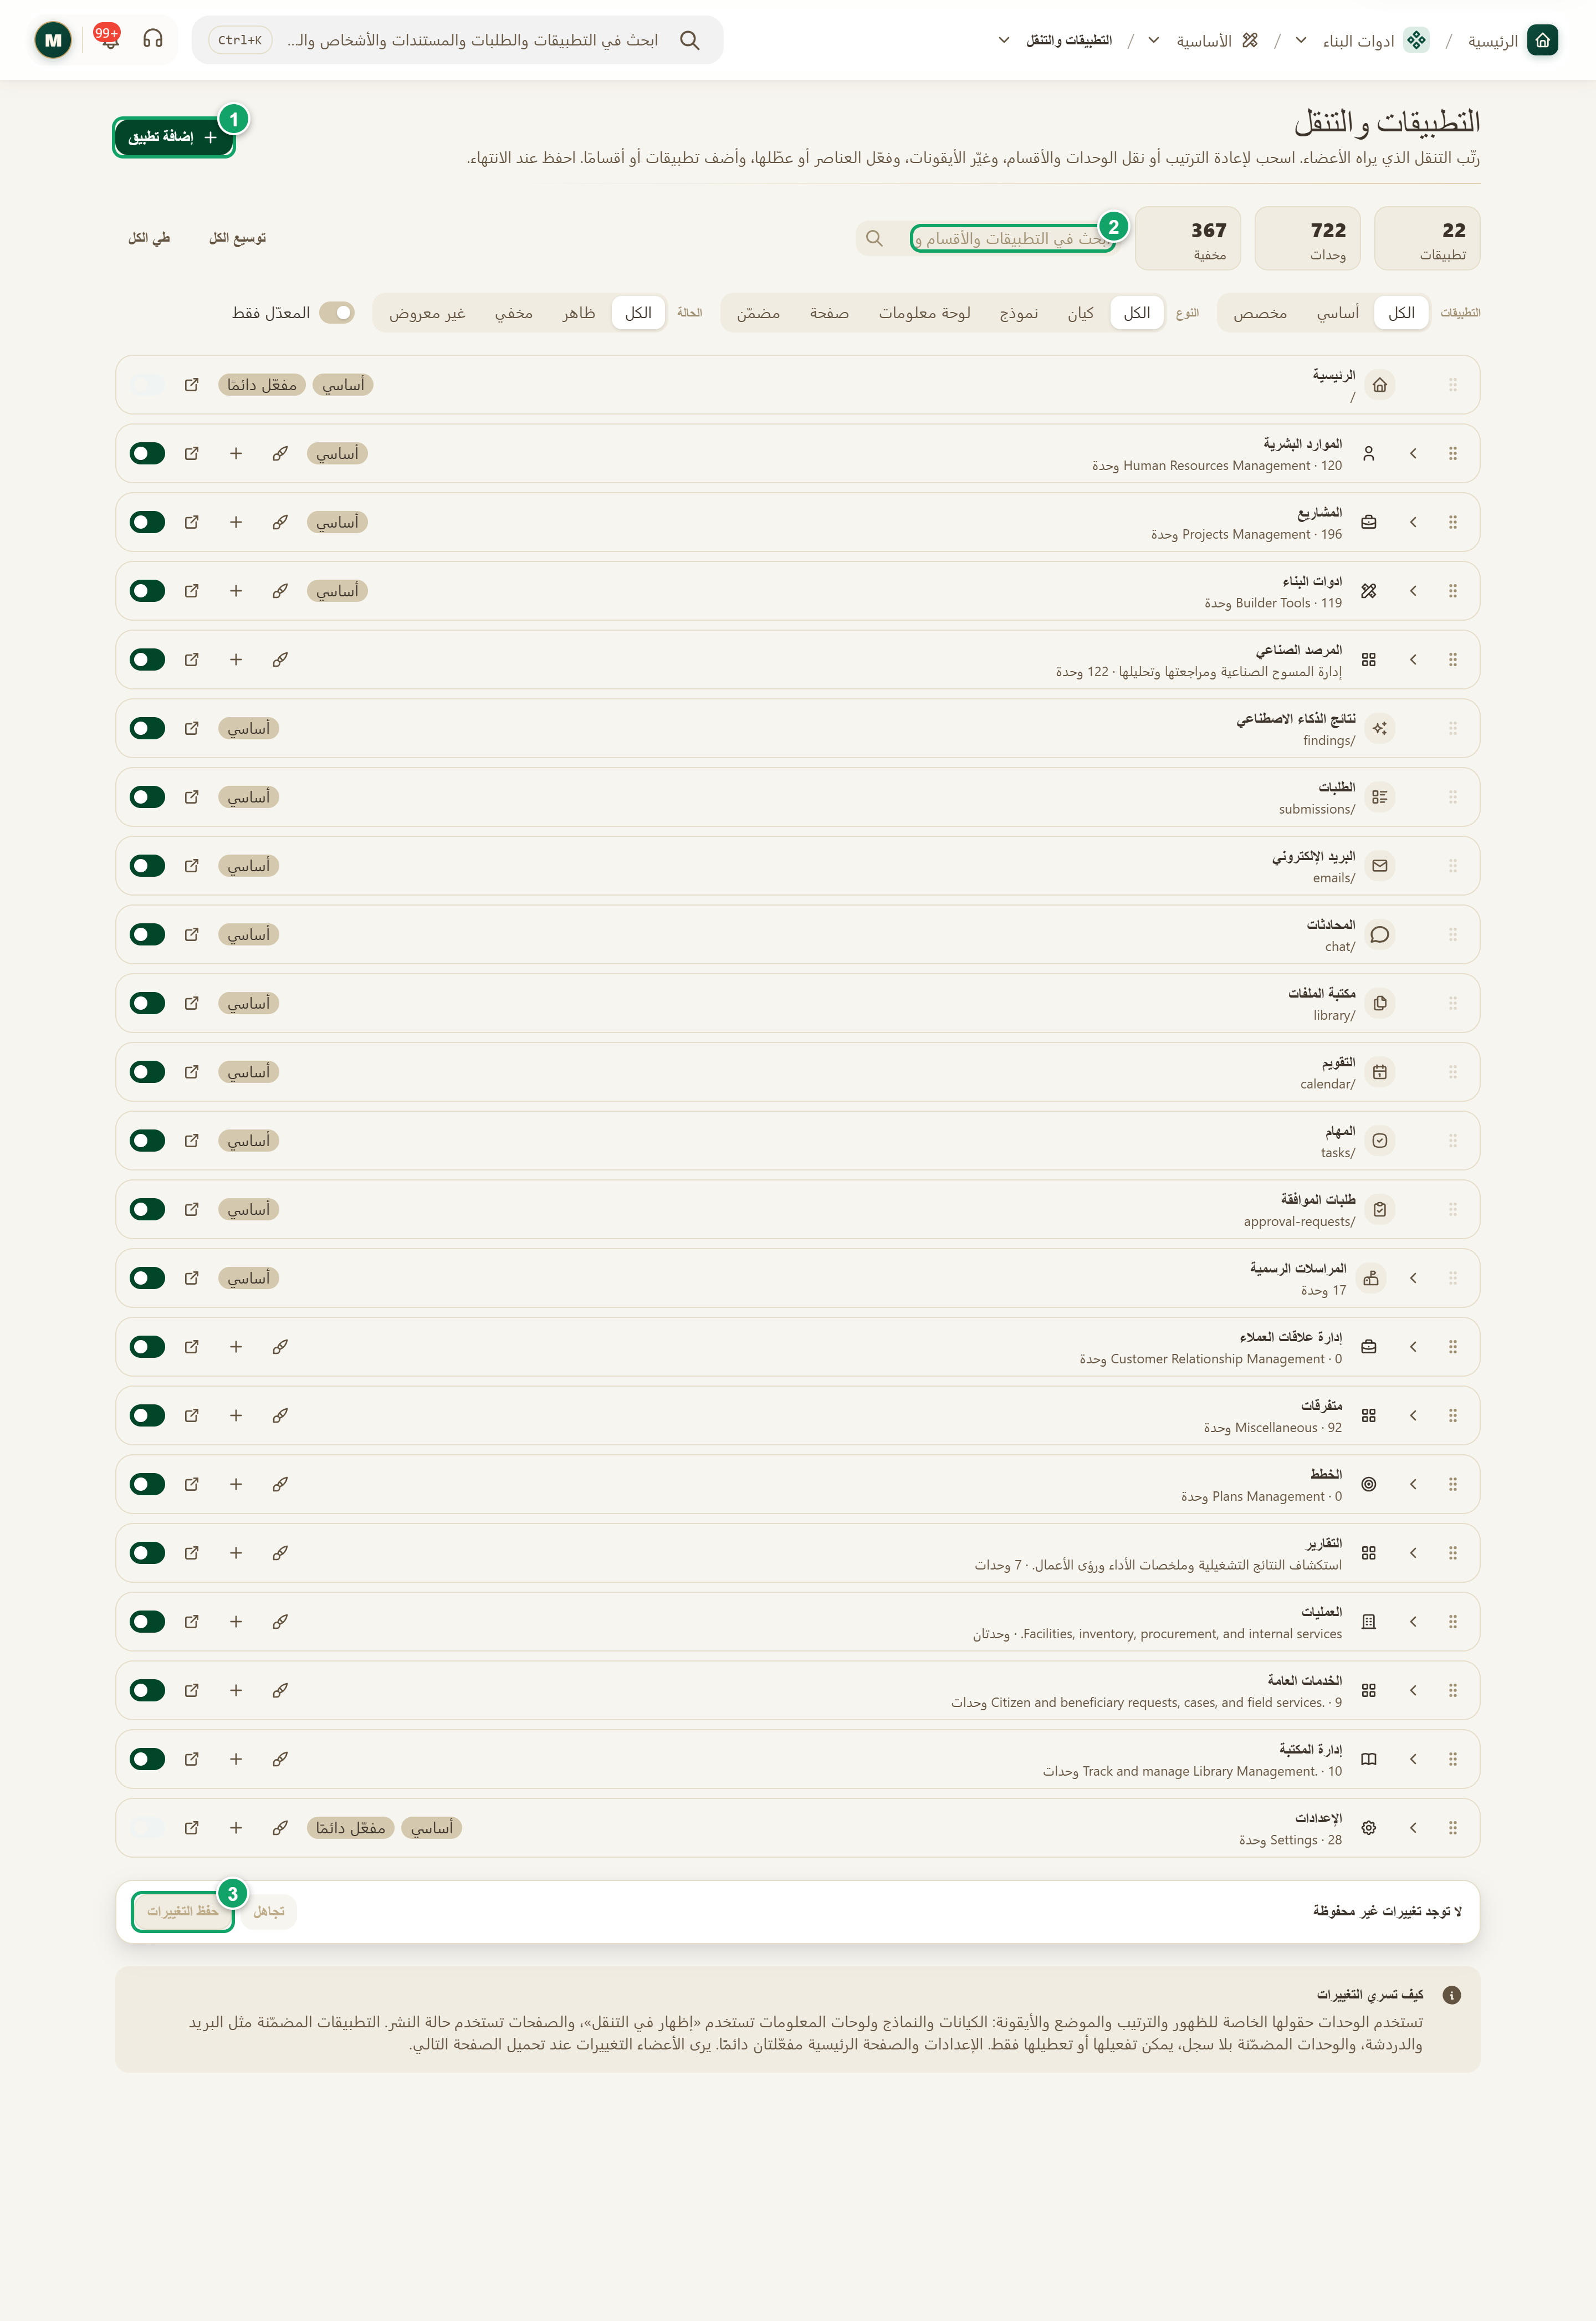
\includegraphics[width=0.95\linewidth,height=0.72\textheight,keepaspectratio]{figures/screens/ch06-navigation-ar.png}
\caption{صفحة «التطبيقات والتنقل»}
\label{fig:builder-navigation-screen}
\shotnote{تعرض الصورة صفحة «التطبيقات والتنقل» في مؤسسة الاختبار، وفيها 22 تطبيقاً لكل منها شاراته ومفتاح ظهوره. وتبقى تغييرات الترتيب والتفعيل مسودة يعرض شريط الحفظ حالتها حتى تحفظها، فتستطيع مراجعتها قبل أن تصل إلى الأعضاء. ① «إضافة تطبيق»: يُنشئ تطبيقاً جديداً ويحفظه فوراً. ② البحث: يجد التطبيق أو القسم أو الوحدة باسمه. ③ مفتاح التطبيق: يُظهره أو يخفيه مع كل ما فيه. ④ «المعدّل فقط»: يعرض ما غيّرته ولم تحفظه. ⑤ «حفظ التغييرات»: يحفظ الترتيب والتفعيل.}
\end{figure}

\begin{table}[H]
\centering
\caption{أجزاء الصفحة}
\label{tab:builder-navigation-data}
\begin{tabularx}{\linewidth}{R{3.6cm} Y}
\rcHeaderRow
\thh{الجزء} & \thh{المحتوى والإجراء}\\
الأرقام والبحث & تعرض الصفحة عدد «تطبيقات» و«وحدات» والعناصر «مخفية». ويجد البحث «ابحث في التطبيقات والأقسام والوحدات» أي عنصر باسمه، ويفتح «توسيع الكل» و«طي الكل» التطبيقات أو يطويها.\\
التصفية & «التطبيقات»: «الكل» أو «أساسي» أو «مخصص»؛ و«النوع»: «كيان» أو «نموذج» أو «لوحة معلومات» أو «صفحة» أو «مضمّن»؛ و«الحالة»: «ظاهر» أو «مخفي» أو «غير معروض»؛ ثم «المعدّل فقط» لعرض ما غيّرته ولم تحفظه. ويعيد «مسح عوامل التصفية» القائمة كاملة.\\
السحب & اسحب التطبيق من مقبضه لتغيّر ترتيبه، واسحب القسم داخل تطبيقه أو إلى تطبيق آخر، واسحب الوحدة داخل قسمها أو إلى قسم آخر.\\
مفاتيح التشغيل & يُظهر المفتاح العنصر أو يخفيه. وإخفاء التطبيق أو القسم يخفي كل ما فيه.\\
شريط الحفظ & يعرض عدد التغييرات غير المحفوظة، وفيه «تجاهل» للتراجع عنها و«حفظ التغييرات» لحفظها.\\
كيف تسري التغييرات & يذكّرك بأن الوحدات تحفظ ظهورها في سجلاتها: أنواع السجلات والنماذج ولوحات المعلومات في «إظهار في التنقل»، والصفحات في حالة نشرها.\\
\end{tabularx}
\end{table}

\begin{table}[H]
\centering
\caption{الشارات في صفوف الشجرة}
\label{tab:builder-navigation-chips}
\begin{tabularx}{\linewidth}{R{3.6cm} Y}
\rcHeaderRow
\thh{الشارة} & \thh{معناها}\\
أساسي & تطبيق مضمّن في النظام، مثل البريد والدردشة. وهذه التطبيقات تُفعَّل أو تُعطَّل فقط، ولا تستقبل وحدات جديدة.\\
مفعّل دائمًا & تطبيق لا يمكن إيقافه، مثل الإعدادات والصفحة الرئيسية، لذلك يكون مفتاحه معطلاً.\\
مخفي أو مسودة & الوحدة نفسها متوقفة. وتظهر «مسودة» للصفحة التي لم تُنشر بعد.\\
معطّل · موروث & الوحدة مفعّلة، لكن تطبيقها أو قسمها متوقف، فلا يراها الأعضاء حتى تشغّل العنصر الأعلى.\\
\end{tabularx}
\end{table}

\begin{rcwarn}[إلى أين يمكن نقل الوحدة؟]
لا يمكن نقل الوحدة إلا إلى قسم له سجل، أي قسم أُضيف من هذه الصفحة أو حُفظ كسجل. فإذا أفلتّ وحدة في قسم مضمّن، تظهر رسالة «هذا التطبيق أو القسم مضمّن ولا يمكنه استقبال وحدات. انقلها إلى قسم له سجل.»، ولا يتغير شيء. أما الوحدات المضمّنة التي لا سجل لها فلا تُسحب أصلاً، ويمكنك إخفاؤها فقط.
\end{rcwarn}

\begin{figure}[H]
\centering
\begin{tikzpicture}[node distance=0.5cm]
\node[entity] (app) {\RL{التطبيق}};
\node[entity,below=0.7cm of app] (section) {\RL{القسم}};
\node[entityOpt,below right=0.7cm and 0.3cm of section] (type) {\RL{نوع سجلات أو نموذج}};
\node[entityOpt,below left=0.7cm and 0.3cm of section] (dash) {\RL{لوحة معلومات أو صفحة}};
\draw[dependsOn] (app) -- (section);
\draw[dependsOnOpt] (section.south) -- ++(0,-0.3) -| (type.north);
\draw[dependsOnOpt] (section.south) -- ++(0,-0.3) -| (dash.north);
\end{tikzpicture}
\rclegend
\caption{كيف يُبنى التنقل}
\label{fig:builder-navigation-tree}
\shotnote{يوضّح الشكل أن التطبيق يضم أقساماً، وأن القسم يضم الوحدات التي يفتحها الأعضاء، مثل أنواع السجلات والنماذج ولوحات المعلومات. لذلك أنشئ التطبيق والقسم أولاً ثم اسحب الوحدة إليه؛ فالتطبيق المضمّن لا يستقبل وحدات جديدة.}
\end{figure}

\subsection{خطوات العمل والتحقق}
\begin{enumerate}
\item افتح «التطبيقات والتنقل»، واكتب اسم الوحدة في البحث، أو اختر نوعها من تصفية «النوع».
\item اسحب الوحدة من مقبضها إلى القسم المطلوب، وأفلتها في الموضع الذي تريده بين وحداته.
\item تأكد من أن مفتاح الوحدة ومفتاحَي قسمها وتطبيقها مشغّلة، وأن الصف لا يحمل شارة «مخفي» أو «معطّل · موروث».
\item فعّل «المعدّل فقط» لتراجع ما غيّرته، ثم اضغط «حفظ التغييرات».
\end{enumerate}

\textbf{تحقق ومعالجة المشكلة:} يجب أن تظهر رسالة «تم حفظ التنقل.»، وأن يعود الشريط إلى «لا توجد تغييرات غير محفوظة»، ثم يرى الأعضاء الترتيب الجديد عند تحميل الصفحة التالي. فإذا لم يظهر العنصر لعضو، فتأكد من أن لديه صلاحية رؤية سجلاته، لأن القسم الذي لا يحتوي عنصراً مسموحاً له لا يظهر. وإذا ظهرت رسالة «تعذّر حفظ التغييرات. يرجى المحاولة مرة أخرى.»، فتحقق من اتصالك واضغط «حفظ التغييرات» مرة أخرى؛ فتعديلاتك تبقى في الصفحة ما لم تضغط «تجاهل».

\clearpage
\section{إضافة التطبيقات والأقسام}
\label{sec:builder-feature-navigation-apps-sections}

عندما تبني عملاً جديداً، فقد لا يناسبه أي تطبيق موجود. لذلك تتيح لك الصفحة إنشاء تطبيق جديد يجمع هذا العمل، ثم إضافة أقسام داخله تصنّف وحداته. ويختلف هذا الإجراء عن الترتيب والتفعيل في أنه يُحفظ فوراً عند الإنشاء، فلا تحتاج بعده إلى «حفظ التغييرات».

ويكفي لكل تطبيق أو قسم عنوانٌ ووصفٌ قصير وأيقونة. ويمكنك لاحقاً تغيير الأيقونة من صفه، وحذف القسم الذي أضفته إذا بقي فارغاً.

\textbf{المسار ومن يستخدمه:} «ادوات البناء» ← «الأساسية» ← «التطبيقات والتنقل» ← «إضافة تطبيق»، أو زر «إضافة قسم» في صف التطبيق. يستخدمه مالك المؤسسة ومسؤولها عند إطلاق عمل جديد.

\begin{rcnote}[مثال: شركة الأفق]
يضغط مسؤول النظام «إضافة تطبيق» ويكتب العنوان «خدمات الفروع» مع وصف يقول إنه يجمع خدمات فرعَي دمشق وحلب، ثم يضغط «إنشاء». بعد ذلك يضيف في التطبيق قسماً باسم «الزيارات» ليضع فيه «طلبات الزيارة». وتطابق هذه الخطوات الأرقام من ① إلى ④ في الصورة.
\end{rcnote}

\begin{figure}[H]
\centering
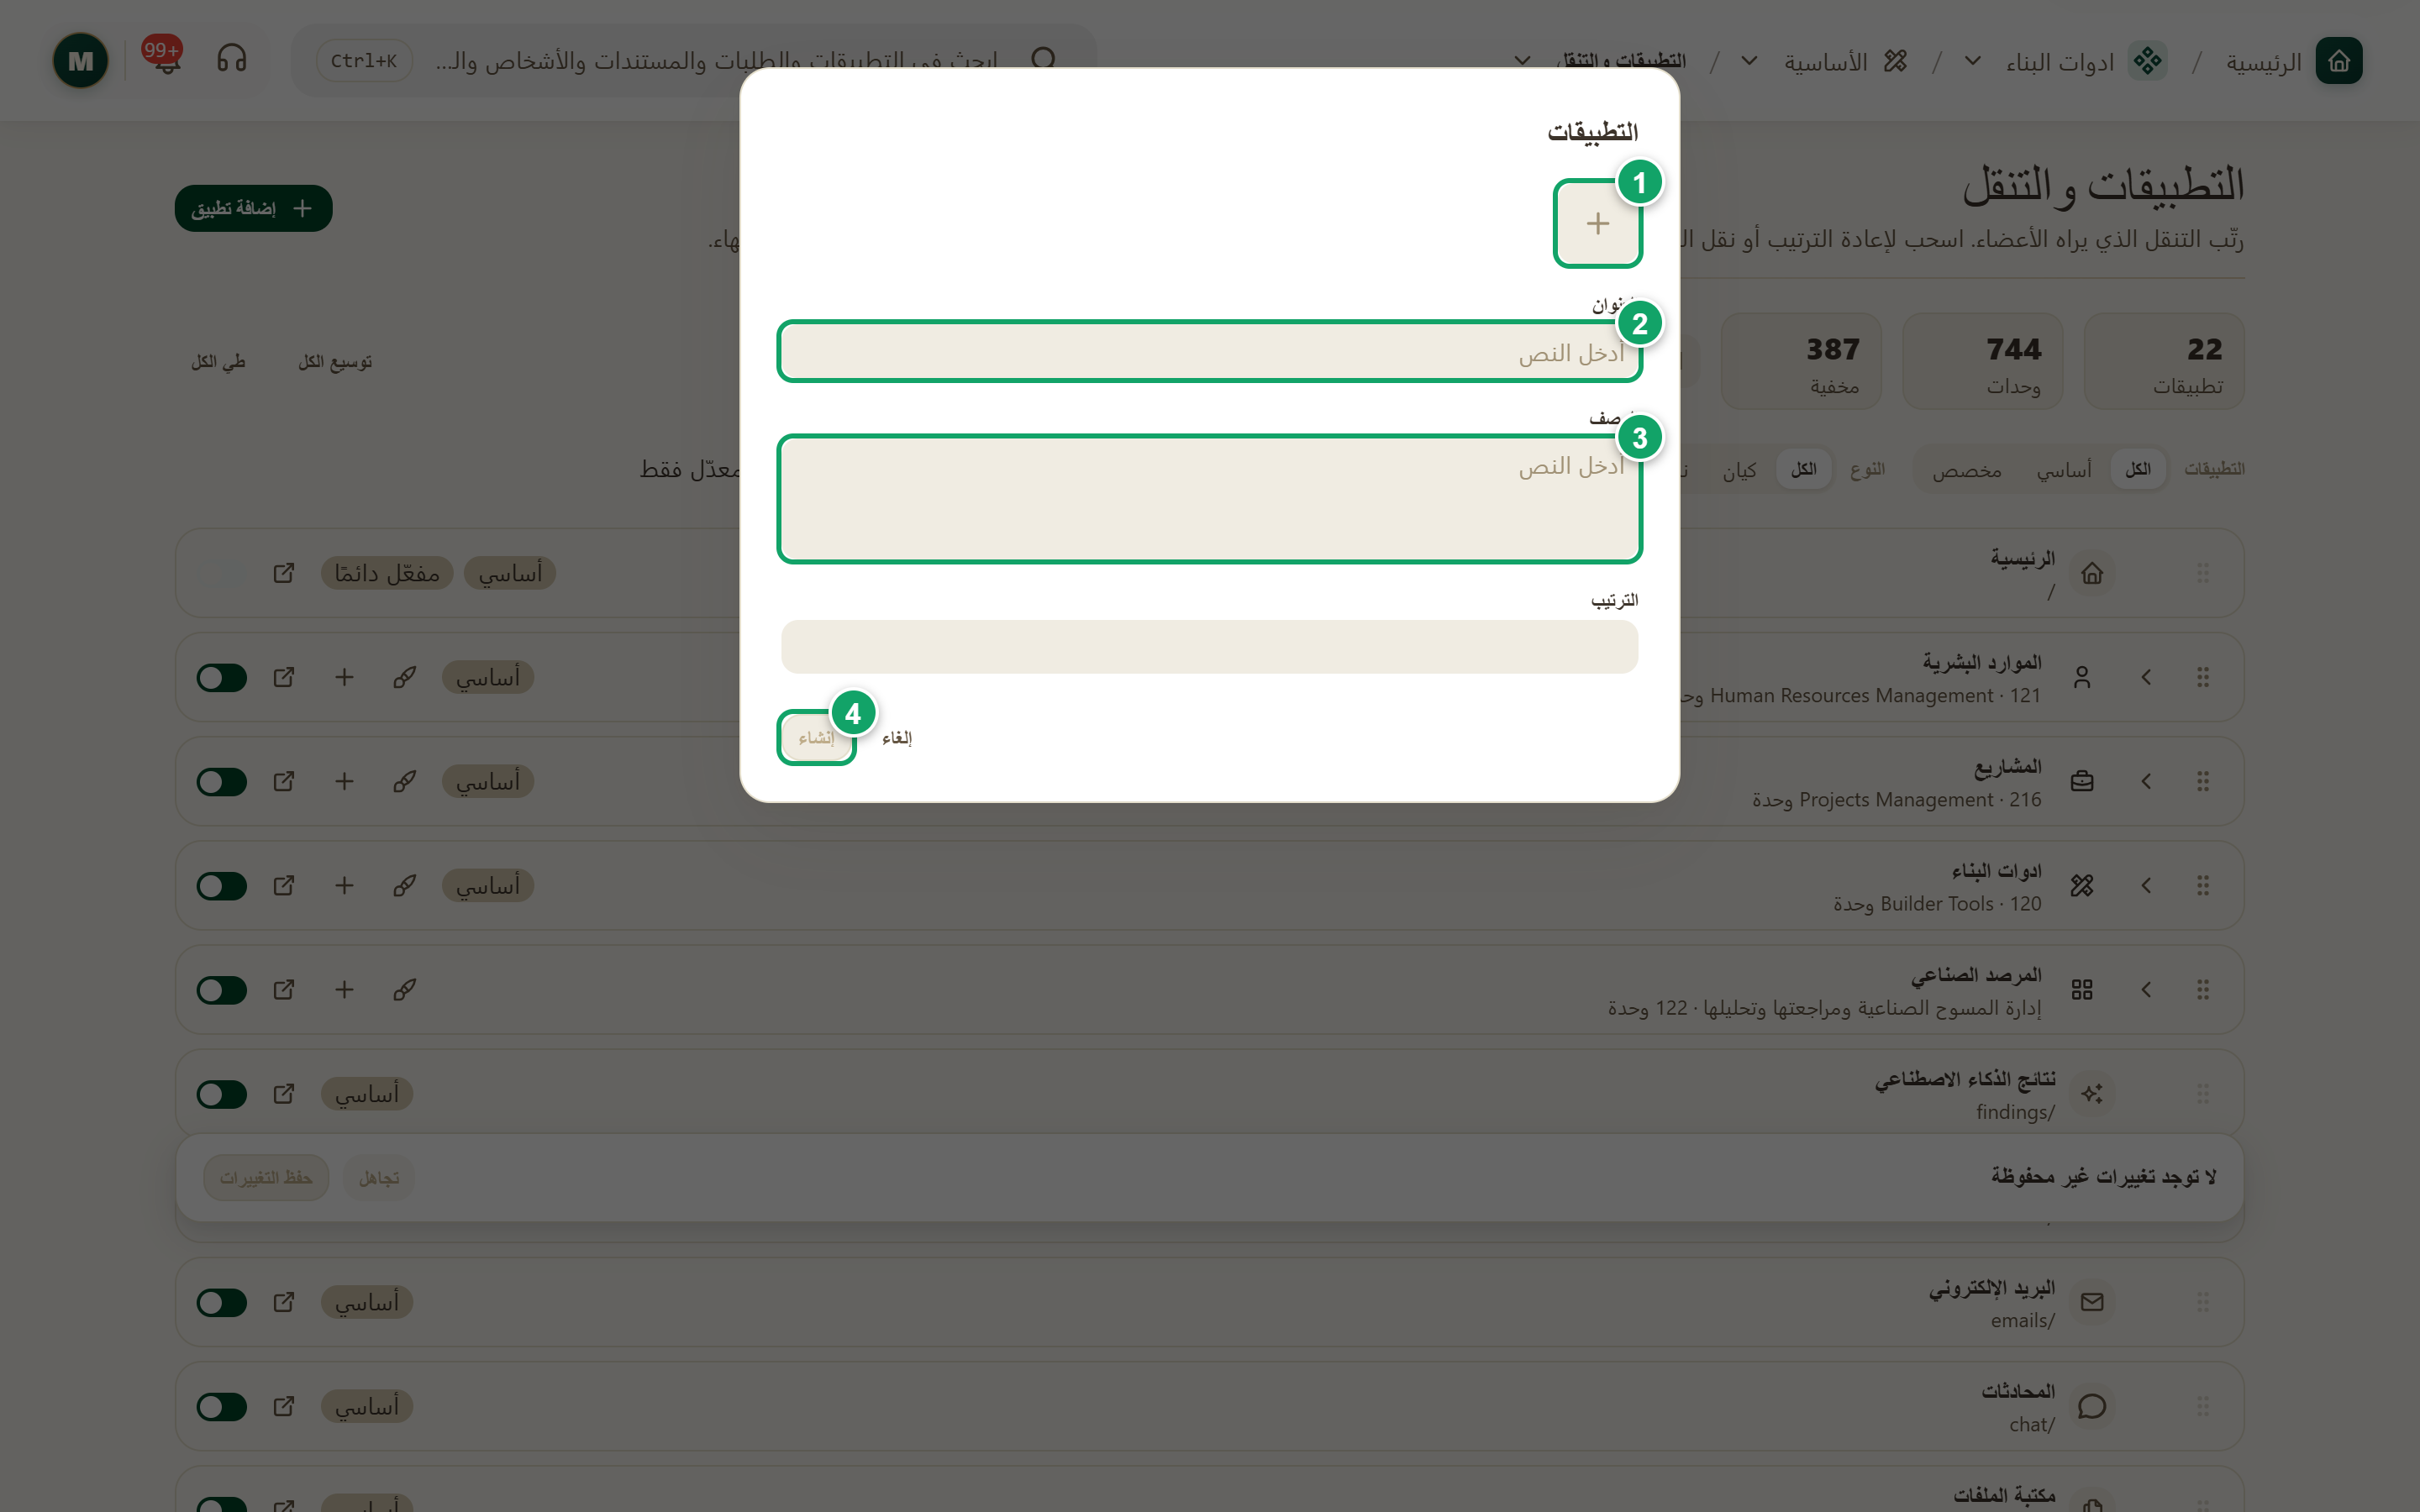
\includegraphics[width=0.95\linewidth,height=0.72\textheight,keepaspectratio]{figures/screens/ch06-nav-add-app-ar.png}
\caption{نافذة إنشاء تطبيق قبل تعبئتها}
\label{fig:builder-navigation-apps-sections-screen}
\shotnote{تعرض الصورة النافذة التي تفتح بعد الضغط على «إضافة تطبيق» في مؤسسة الاختبار، وهي فارغة لأن الالتقاط لم يُنشئ شيئاً. وتفتح النافذة نفسها من زر «إضافة قسم» في صف التطبيق، ويُحفظ ما تنشئه فور الضغط على «إنشاء» دون «حفظ التغييرات». ① منتقي الأيقونة: يختار أيقونة التطبيق أو القسم. ② «العنوان»: الاسم الذي يظهر في القائمة. ③ «الوصف»: جملة إلزامية من 12 حرفاً وكلمتين على الأقل. ④ «إنشاء»: يبقى معطلاً حتى يكتمل العنوان والوصف.}
\end{figure}

\begin{table}[H]
\centering
\caption{نافذة الإنشاء}
\label{tab:builder-navigation-apps-sections-dialog}
\begin{tabularx}{\linewidth}{R{3.6cm} Y}
\rcHeaderRow
\thh{الحقل} & \thh{ما تكتبه فيه}\\
الأيقونة & اختر أيقونة من المنتقي. وإذا لم تختر شيئاً، يأخذ التطبيق أو القسم أيقونة افتراضية.\\
العنوان & الاسم الذي يظهر في القائمة، ويمكن كتابته بكل لغة. وهو حقل إلزامي.\\
الوصف & جملة تشرح الغرض، وهي إلزامية أيضاً. ويجب أن تتكون من 12 حرفاً وكلمتين على الأقل، وإلا ظهرت «صِف في 12 حرفاً وكلمتين على الأقل.».\\
الترتيب & رقم اختياري يحدد موضع العنصر بين نظرائه. ويمكنك تعديل الموضع لاحقاً بالسحب.\\
إنشاء وإلغاء & يبقى «إنشاء» معطلاً حتى تكتب العنوان ووصفاً صالحاً، أما «إلغاء» فيغلق النافذة دون حفظ.\\
\end{tabularx}
\end{table}

\begin{table}[H]
\centering
\caption{أزرار الصف بعد الإنشاء}
\label{tab:builder-navigation-apps-sections-row}
\begin{tabularx}{\linewidth}{R{3.6cm} Y}
\rcHeaderRow
\thh{الزر} & \thh{ما يفعله}\\
إضافة قسم & يظهر في صف التطبيق الذي له سجل، ويفتح النافذة نفسها لإنشاء قسم داخله. ولا يظهر في التطبيقات المضمّنة التي لا أقسام لها.\\
تغيير الأيقونة & يظهر عند أيقونة التطبيق أو القسم أو الوحدة. والأيقونة الجديدة تدخل المسودة، فتحتاج إلى «حفظ التغييرات».\\
حذف القسم & يظهر فقط للقسم الذي أُضيف من هذه الصفحة ولا يحتوي أي وحدة. ويُحذف فوراً للجميع بعد التأكيد، ولا يمكن التراجع عن ذلك.\\
\end{tabularx}
\end{table}

\begin{figure}[H]
\centering
\begin{tikzpicture}[node distance=0.5cm]
\node[stepBox] (a) {\RL{إضافة تطبيق}};
\node[stepBox,below=of a] (b) {\RL{العنوان والوصف والأيقونة}};
\node[stepBox,below=of b] (c) {\RL{إنشاء}};
\node[stepBox,below=of c] (d) {\RL{إضافة قسم في صف التطبيق}};
\node[stepBox,below=of d] (e) {\RL{سحب الوحدات إلى القسم}};
\node[stepBox,below=of e] (f) {\RL{حفظ التغييرات}};
\draw[flowsTo] (a) -- (b);
\draw[flowsTo] (b) -- (c);
\draw[flowsTo] (c) -- (d);
\draw[flowsTo] (d) -- (e);
\draw[flowsTo] (e) -- (f);
\end{tikzpicture}
\rclegend
\caption{من تطبيق جديد إلى قائمة جاهزة}
\label{fig:builder-navigation-apps-sections-flow}
\shotnote{يجمع المخطط نوعين من الحفظ: فالتطبيق والقسم يُحفظان عند الضغط على «إنشاء»، أما نقل الوحدات إلى القسم فيبقى مسودة حتى «حفظ التغييرات». لذلك لا تكتمل القائمة الجديدة إلا بعد الخطوة الأخيرة، لأن القسم الفارغ لا يعرض للأعضاء شيئاً.}
\end{figure}

\subsection{خطوات العمل والتحقق}
\begin{enumerate}
\item افتح «التطبيقات والتنقل» واضغط «إضافة تطبيق».
\item اختر أيقونة، واكتب «العنوان» و«الوصف»، ثم اضغط «إنشاء».
\item ابحث عن التطبيق الجديد، واضغط زر «إضافة قسم» في صفه، واملأ النافذة بالطريقة نفسها، ثم اضغط «إنشاء».
\item اسحب الوحدات إلى القسم الجديد، واضغط «حفظ التغييرات».
\item إذا أنشأت قسماً بالخطأ وبقي فارغاً، فاضغط زر حذفه في صفه، ثم «حذف» في نافذة التأكيد.
\end{enumerate}

\textbf{تحقق ومعالجة المشكلة:} بعد إنشاء القسم تظهر رسالة «تمت إضافة القسم وحفظه مباشرةً، فلا حاجة للضغط على حفظ.»، ويظهر القسم تحت تطبيقه مع العبارة «لا توجد وحدات في هذا القسم. اسحب وحدة إلى هنا.». فإذا بقي «إنشاء» معطلاً، فأطل الوصف ليصبح جملة واضحة. وإذا لم تجد زر الحذف في قسم ما، فإما أن القسم مضمّن أو أن فيه وحدات؛ فانقل وحداته أولاً واحفظ، ثم احذفه.

\clearpage
\section{هوية التطبيق}
\label{sec:builder-feature-navigation-identity}

تمنح «هوية التطبيق» التطبيقَ اسماً وشعاراً ولوناً خاصاً به. فعندما يعمل العضو داخل هذا التطبيق، تحل هويته محل هوية المؤسسة في الشريط العلوي، ثم تعود هوية المؤسسة في بقية الأماكن. ويفيد ذلك عندما يخدم التطبيق جهة أو عميلاً بعينه، فيعرف المستخدم أين يعمل.

وتضم النافذة أيضاً «الوضع المركّز»، وهو يقصر ما يراه بعض الأعضاء على هذا التطبيق وحده. وتُحفظ الهوية فور الضغط على «حفظ» في النافذة، دون الحاجة إلى «حفظ التغييرات».

\textbf{المسار ومن يستخدمه:} «ادوات البناء» ← «الأساسية» ← «التطبيقات والتنقل» ← زر «هوية التطبيق» في صف التطبيق. يظهر الزر للتطبيقات التي لها سجل، ويستخدمه مالك المؤسسة ومسؤولها.

\begin{rcnote}[مثال: شركة الأفق]
يفتح مسؤول النظام «هوية التطبيق» لتطبيق «خدمات الفروع»، ويكتب في «الاسم في الشريط العلوي» «فرع حلب»، ويختار لوناً أخضر داكناً من الألوان الجاهزة، ثم يضغط «حفظ». فيرى عمر حداد هذا الاسم واللون كلما فتح التطبيق. ويكتب الاسم في ① ويحفظ من ⑤.
\end{rcnote}

\begin{figure}[H]
\centering
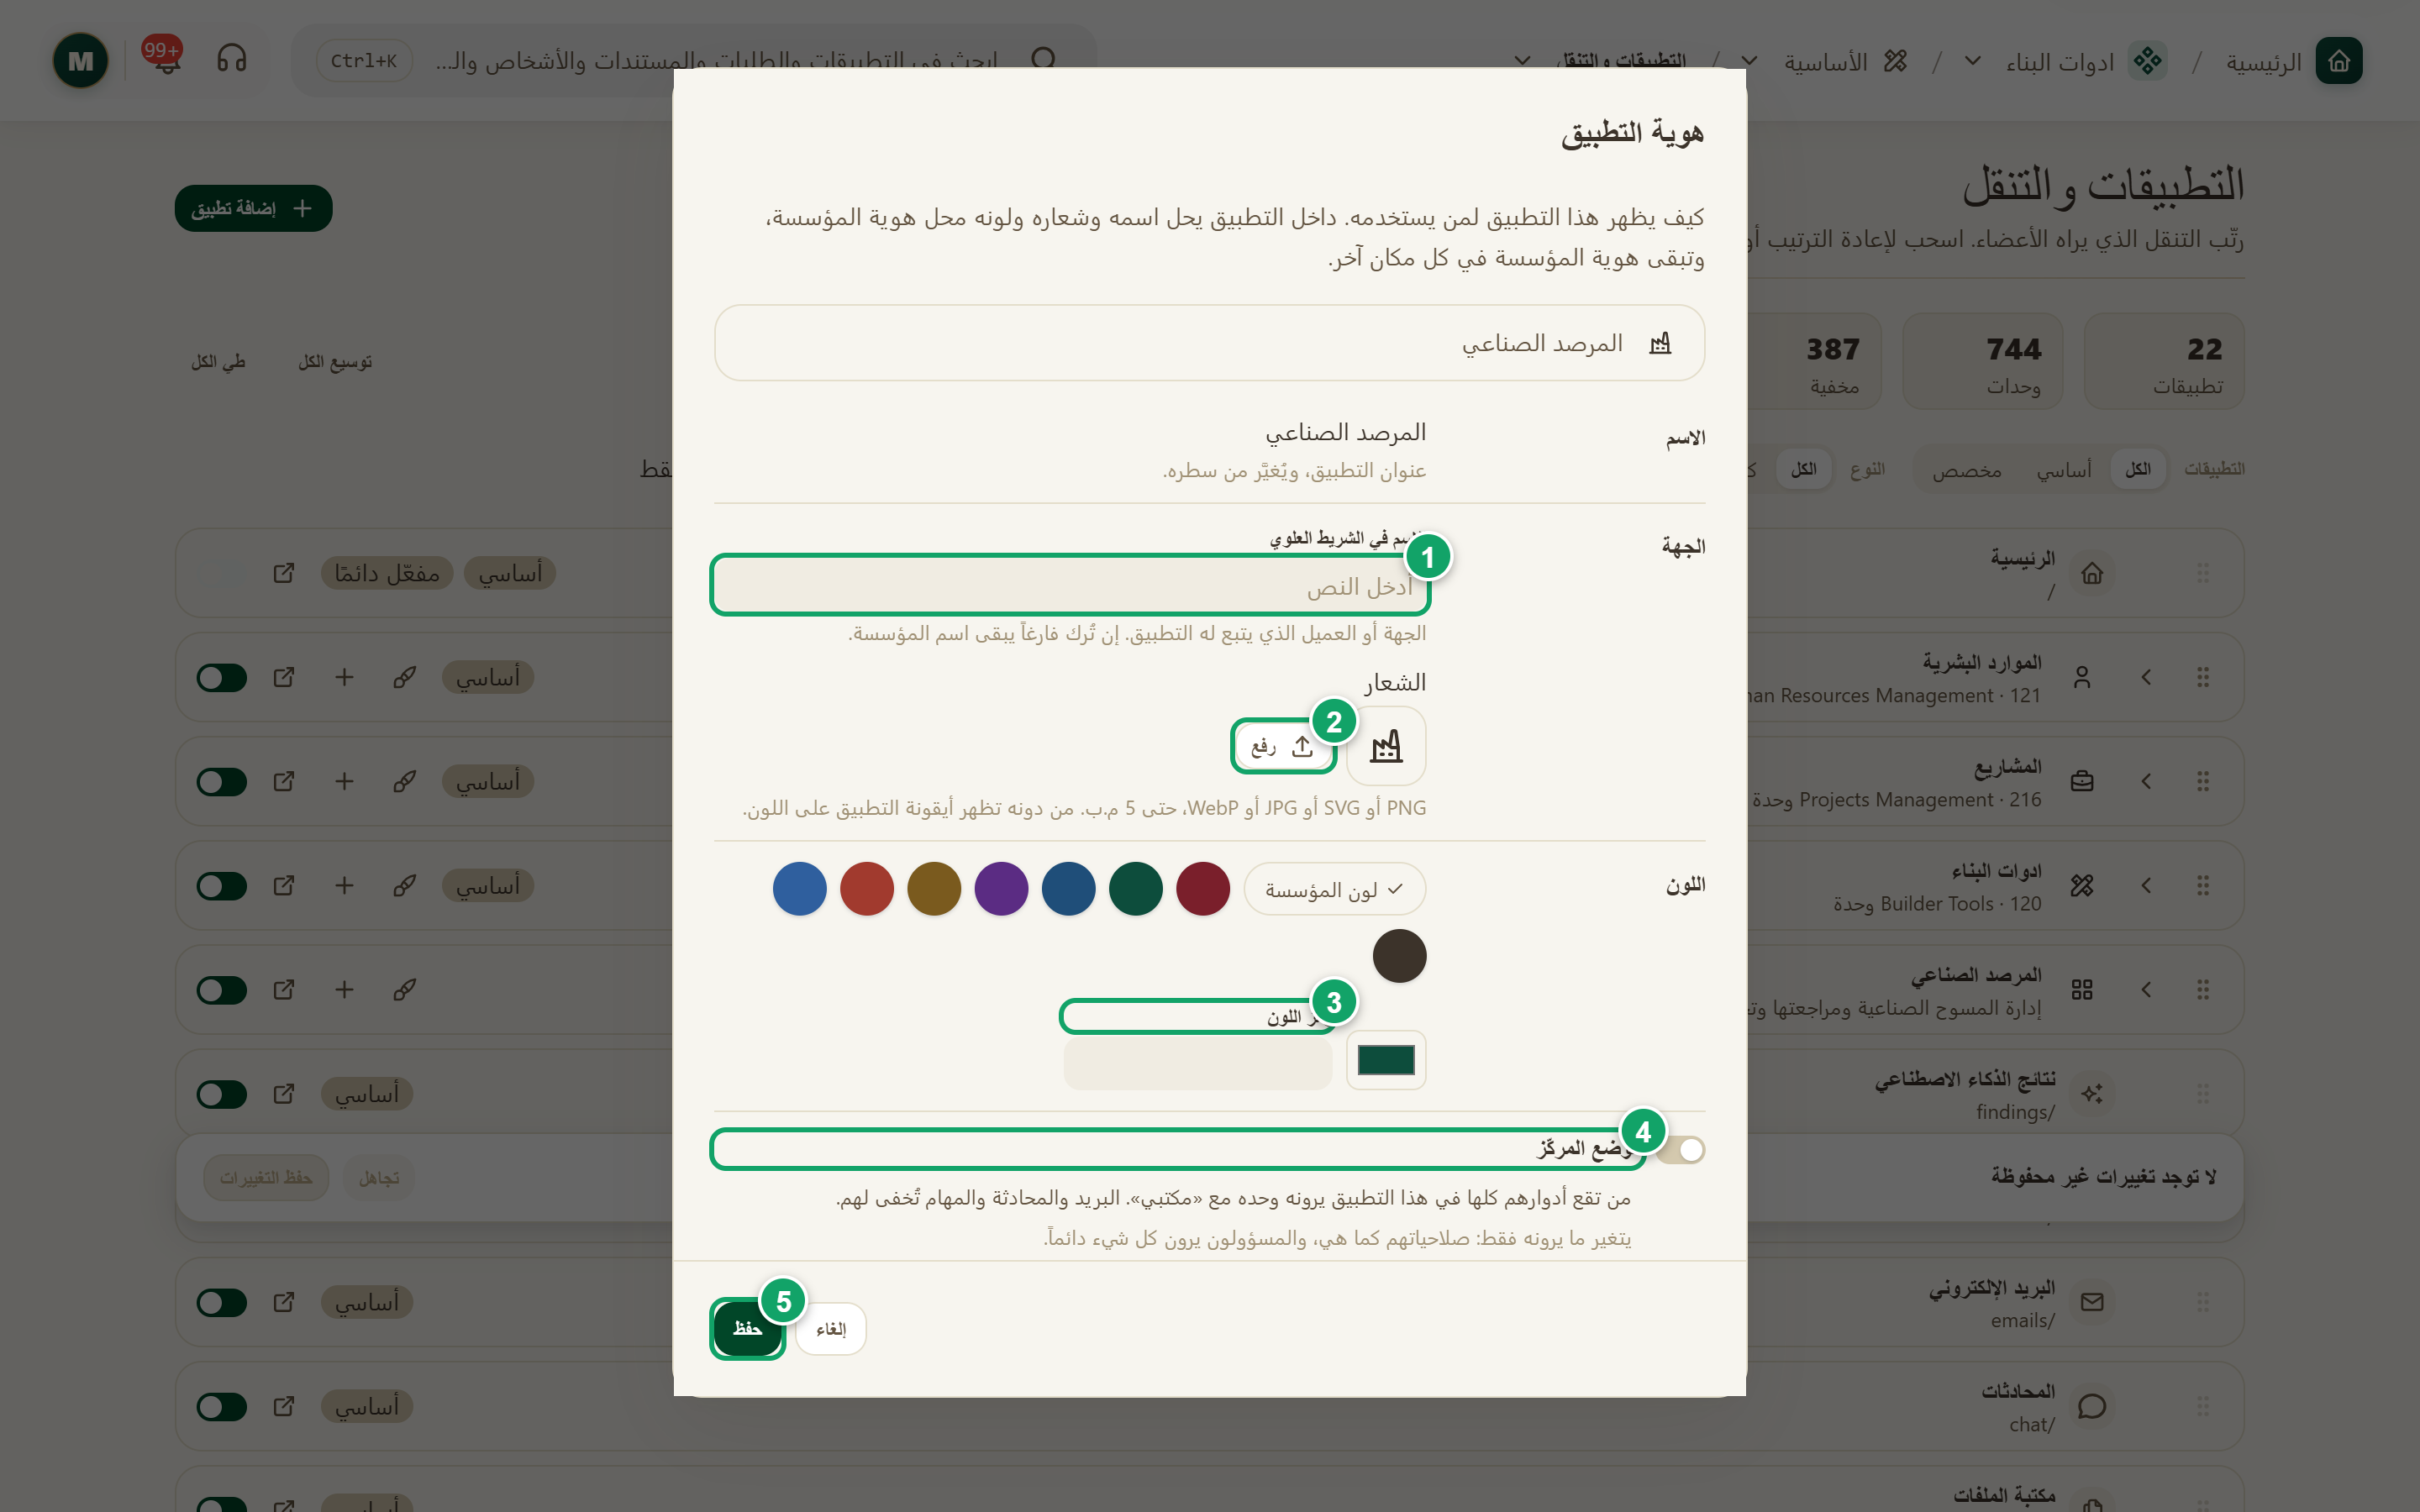
\includegraphics[width=0.95\linewidth,height=0.72\textheight,keepaspectratio]{figures/screens/ch06-nav-identity-ar.png}
\caption{نافذة «هوية التطبيق»}
\label{fig:builder-navigation-identity-screen}
\shotnote{تعرض الصورة نافذة «هوية التطبيق» لتطبيق «المرصد الصناعي» في مؤسسة الاختبار قبل أي تعديل، وتبدأ بمعاينة تتغير مع كل اختيار. وتجمع النافذة الاسم والشعار واللون والوضع المركّز، ثم تحفظها معاً دون الحاجة إلى «حفظ التغييرات». ① «الاسم في الشريط العلوي»: اسم الجهة التي يتبعها التطبيق. ② «رفع»: يرفع صورة الشعار. ③ «رمز اللون»: لون مخصص بالصيغة \en{\#RRGGBB}، ويمكنك بدلاً منه اختيار أحد الألوان الجاهزة. ④ «الوضع المركّز»: يقصر ما يراه أعضاء التطبيق عليه وحده. ⑤ «حفظ»: يحفظ الهوية فوراً.}
\end{figure}

\begin{table}[H]
\centering
\caption{محتوى نافذة «هوية التطبيق»}
\label{tab:builder-navigation-identity-fields}
\begin{tabularx}{\linewidth}{R{3.6cm} Y}
\rcHeaderRow
\thh{الجزء} & \thh{ما يحدده}\\
معاينة & تعرض الشعار واللون والاسم معاً كما ستظهر في الشريط العلوي، وتتغير مع كل اختيار.\\
الاسم & عنوان التطبيق للعرض فقط، ولا يُعدَّل من هذه النافذة.\\
الاسم في الشريط العلوي & اسم الجهة أو العميل الذي يتبع له التطبيق، بكل لغة. وإذا تُرك فارغاً يبقى اسم المؤسسة.\\
الشعار & صورة بصيغة \en{PNG} أو \en{SVG} أو \en{JPG} أو \en{WebP} لا يتجاوز حجمها 5 ميغابايت، ترفعها بزر «رفع» وتغيّرها بزر «استبدال» أو تحذفها بزر «إزالة». ومن دونها تظهر أيقونة التطبيق على اللون.\\
اللون & «لون المؤسسة»، أو أحد ثمانية ألوان جاهزة، أو «لون مخصص» تختاره أو تكتب «رمز اللون» بالصيغة \en{\#RRGGBB}. ويظهر تحذير إذا صعبت قراءة النص الأبيض على اللون.\\
الوضع المركّز & من تقع أدوارهم كلها داخل هذا التطبيق يرونه وحده مع «مكتبي»، ويُخفى عنهم البريد والمحادثة والمهام. ولا تتغير صلاحياتهم، ويرى المسؤولون كل شيء دائماً.\\
يبقى لهم & يظهر عند تشغيل الوضع المركّز، وتختار منه ما يبقى ظاهراً لهؤلاء الأعضاء: «المهام» و«التقويم» و«البريد» و«المحادثة» و«المكتبة» و«ردود النماذج» و«الموارد البشرية» و«المشاريع».\\
\end{tabularx}
\end{table}

\begin{rcwarn}[الوضع المركّز يغيّر ما يُعرض فقط]
لا يمنح الوضع المركّز صلاحية ولا يسحبها، بل يخفي التطبيقات الأخرى عن الأعضاء الذين تقع أدوارهم كلها في هذا التطبيق. فإذا كان لعضو دور في تطبيق آخر، فلن يتأثر بهذا الوضع. ويظهر بجانب التطبيق في الشجرة شارة «مركّز» ما دام الوضع مفعّلاً.
\end{rcwarn}

\begin{figure}[H]
\centering
\begin{tikzpicture}[node distance=0.5cm]
\node[stepBox] (a) {\RL{زر هوية التطبيق}};
\node[stepBox,below=of a] (b) {\RL{الاسم في الشريط العلوي}};
\node[stepBox,below=of b] (c) {\RL{الشعار واللون}};
\node[stepBox,below=of c] (d) {\RL{الوضع المركّز عند الحاجة}};
\node[stepBox,below=of d] (e) {\RL{مراجعة المعاينة ثم حفظ}};
\draw[flowsTo] (a) -- (b);
\draw[flowsTo] (b) -- (c);
\draw[flowsTo] (c) -- (d);
\draw[flowsTo] (d) -- (e);
\end{tikzpicture}
\rclegend
\caption{ضبط هوية التطبيق}
\label{fig:builder-navigation-identity-flow}
\shotnote{يتبع المخطط ترتيب أجزاء النافذة، ويضع المعاينة قبل الحفظ مباشرة لأنها تريك النتيجة كما ستظهر في الشريط العلوي. وخطوة الوضع المركّز اختيارية، فاتركها إذا كان أعضاء التطبيق يحتاجون إلى بقية التطبيقات في عملهم اليومي.}
\end{figure}

\subsection{خطوات العمل والتحقق}
\begin{enumerate}
\item افتح «التطبيقات والتنقل»، وابحث عن التطبيق، واضغط زر «هوية التطبيق» في صفه.
\item اكتب «الاسم في الشريط العلوي» إذا كان التطبيق يتبع جهة غير المؤسسة.
\item ارفع شعاراً بزر «رفع» إن وُجد، واختر لوناً جاهزاً أو اكتب «رمز اللون».
\item شغّل «الوضع المركّز» إذا أردت أن يرى أعضاء التطبيق هذا التطبيق وحده، واختر من «يبقى لهم» ما يحتاجون إليه.
\item راجع «معاينة»، ثم اضغط «حفظ».
\end{enumerate}

\textbf{تحقق ومعالجة المشكلة:} يجب أن تظهر رسالة «حُفظت هوية التطبيق.»، وأن تظهر الهوية في الشريط العلوي عند فتح التطبيق. فإذا بقي «حفظ» معطلاً، فصحّح «رمز اللون» ليكون بالصيغة \en{\#RRGGBB} أو أفرغ الحقل. وإذا ظهرت «حجم الشعار أكبر من 5 م.ب.»، فصغّر الصورة ثم ارفعها مرة أخرى.

\clearpage
\section{إضافة طريقة عرض إلى القائمة}
\label{sec:builder-feature-navigation-views}

طريقة العرض المحفوظة هي قائمة سجلات بتصفية وترتيب جاهزين، مثل «الطلبات التي تنتظر المراجعة». ويمكنك أن تضعها عنصراً مستقلاً في قسم من القائمة، فيفتحها العضو مباشرة دون أن يفتح القائمة الكاملة ثم يختار التصفية. ويمكن أن يظهر بجانبها عدد السجلات الحالي، فيعرف العضو حجم العمل قبل أن يفتحها.

وتُضاف طريقة العرض مسودةً، ولا يراها الأعضاء حتى تشغّل مفتاحها في الشجرة وتحفظ التغييرات.

\textbf{المسار ومن يستخدمه:} «ادوات البناء» ← «الأساسية» ← «التطبيقات والتنقل» ← زر «إضافة طريقة عرض إلى…» في صف القسم. يظهر الزر عندما تكون ميزة «طرق العرض في القوائم» مفعّلة في «التنقل حسب العمل»، وللأقسام التي لها سجل فقط.

\begin{rcnote}[مثال: شركة الأفق]
يضيف مسؤول النظام إلى قسم «الزيارات» طريقة العرض المحفوظة «بانتظار المراجعة» من «طلبات الزيارة»، ويشغّل «إظهار العدد الحالي» بلون «تنبيه». وبعد نشرها ترى سارة الخطيب عدد الطلبات التي تنتظرها بجانب اسمها في القائمة. ويختار النوع من ① ويشغّل العدد من ③ ويختار لونه من ④.
\end{rcnote}

\begin{figure}[H]
\centering
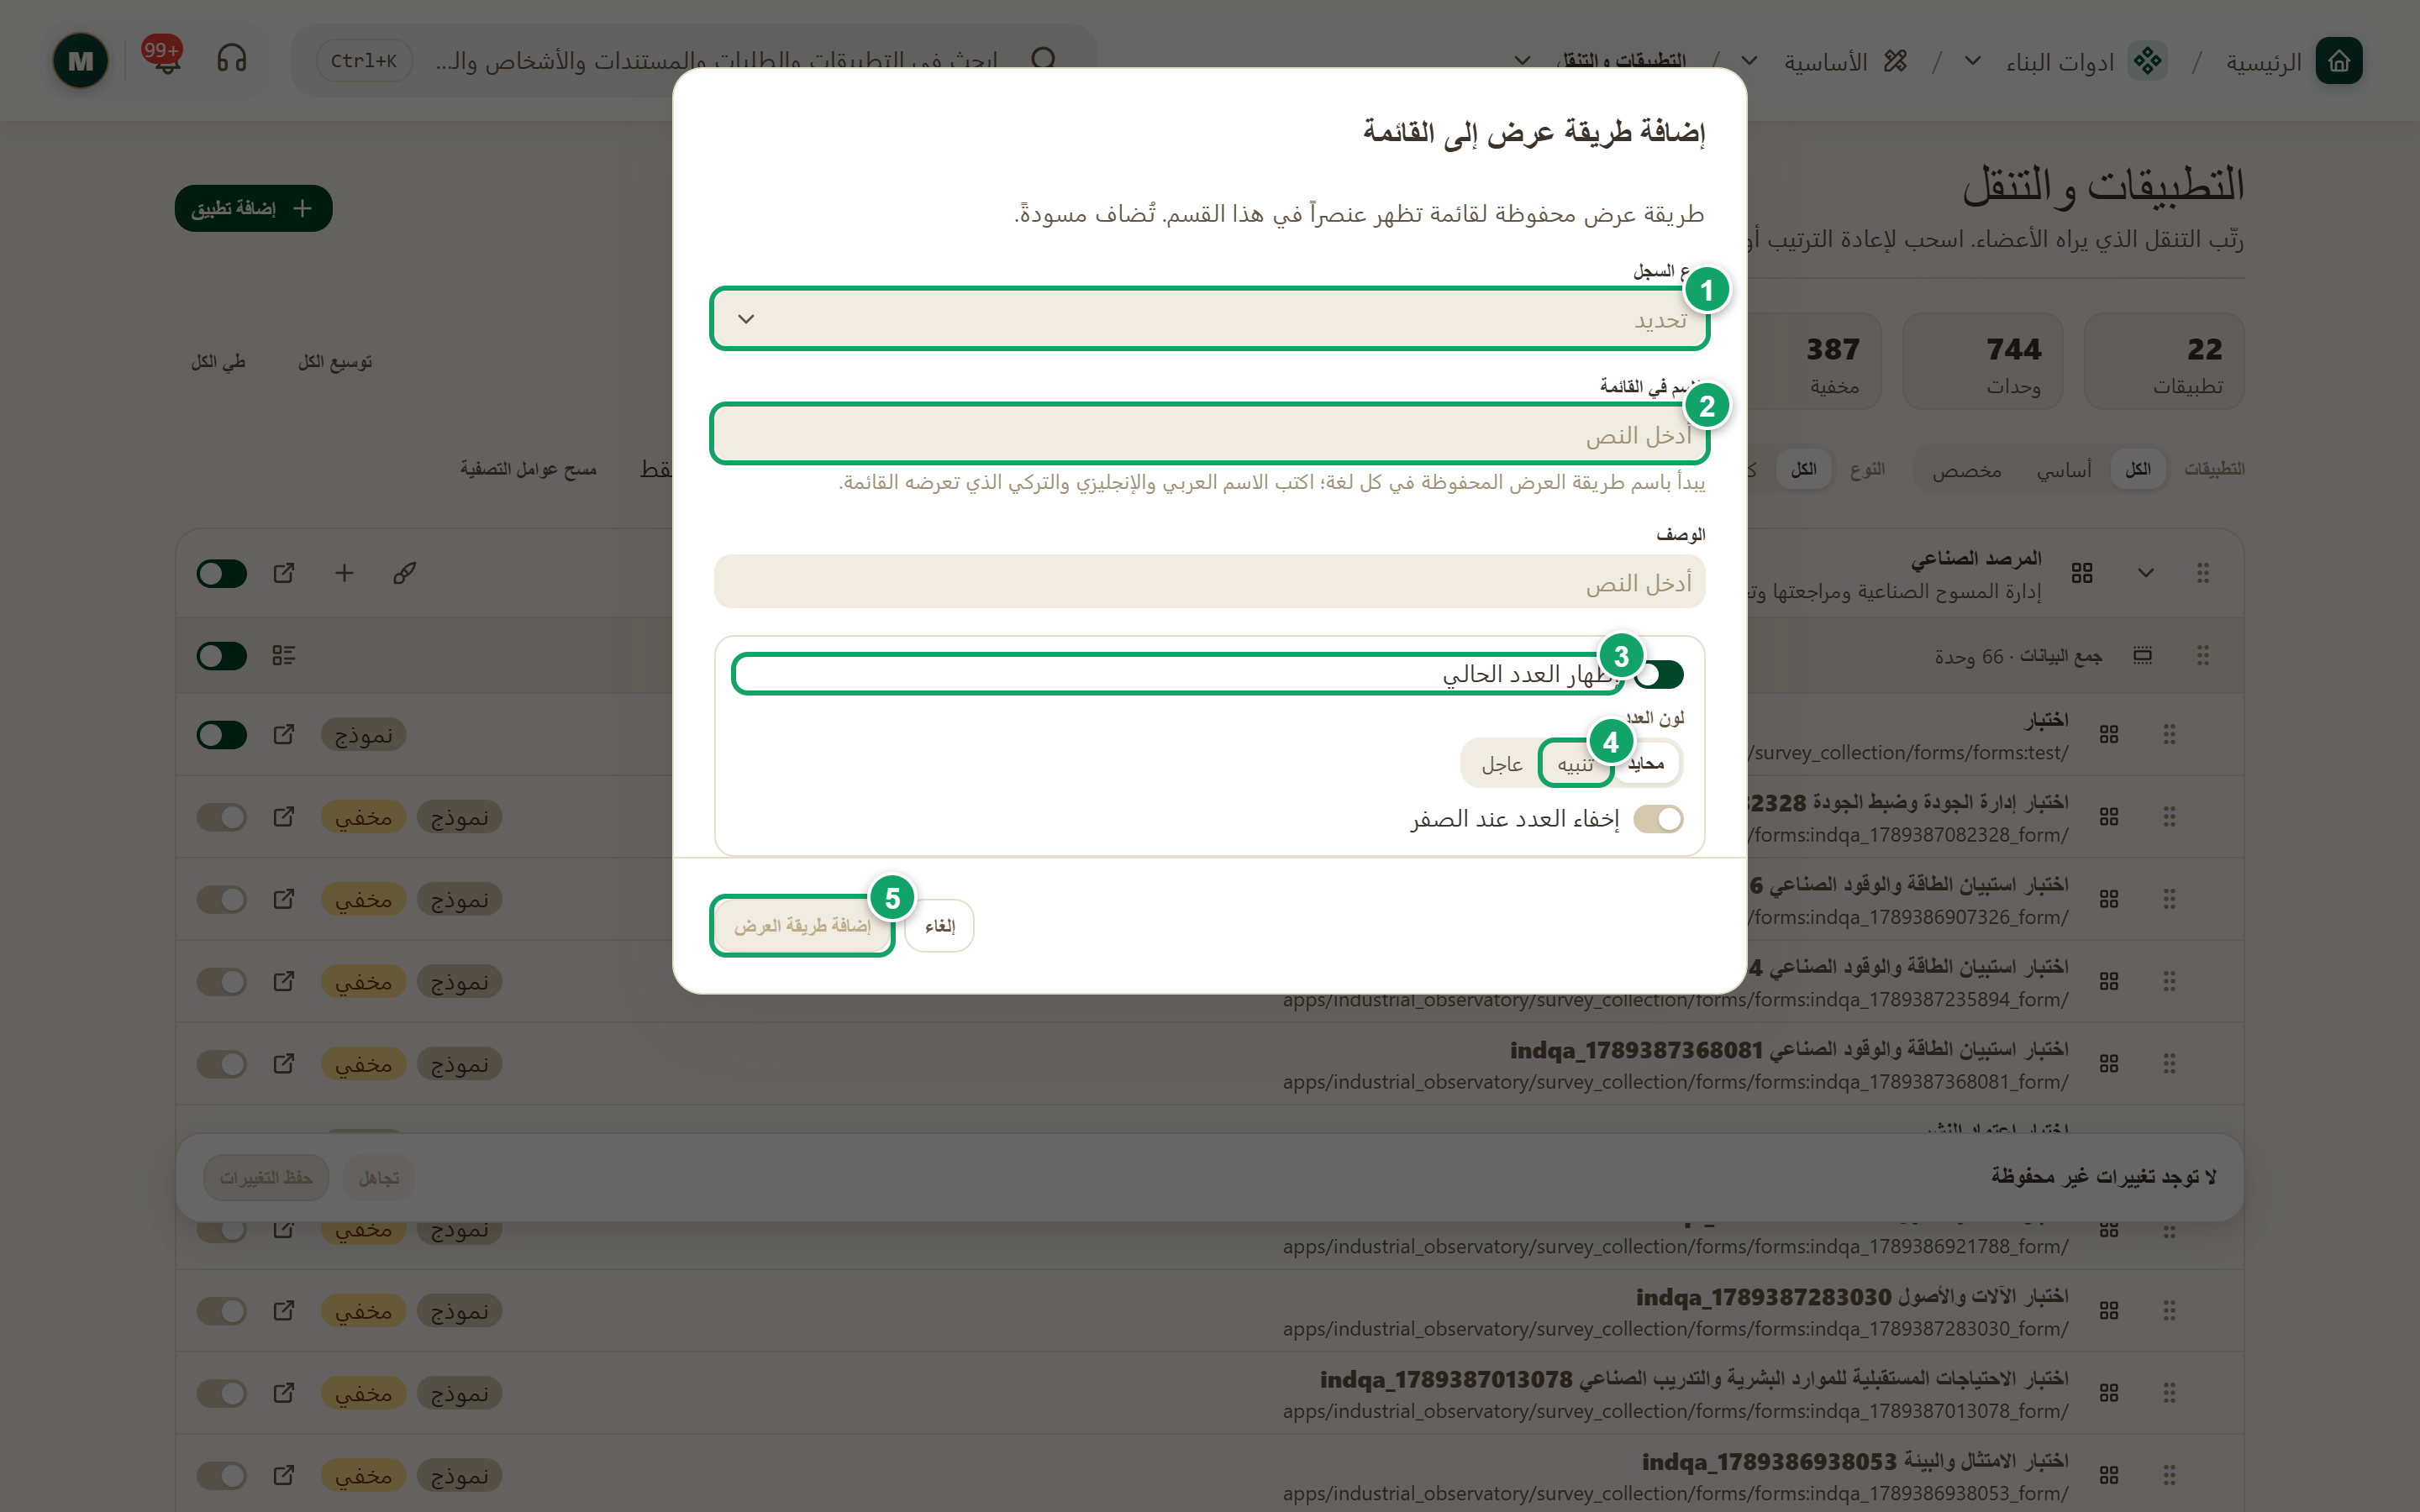
\includegraphics[width=0.95\linewidth,height=0.72\textheight,keepaspectratio]{figures/screens/ch06-nav-add-view-ar.png}
\caption{نافذة «إضافة طريقة عرض إلى القائمة»}
\label{fig:builder-navigation-views-screen}
\shotnote{تعرض الصورة النافذة بعد الضغط على زر الإضافة في صف قسم «جمع البيانات» من مؤسسة الاختبار، وقبل اختيار نوع السجل الذي تعتمد عليه قائمة طرق العرض المحفوظة. ويظهر فيها «إظهار العدد الحالي» مشغّلاً افتراضياً، والعنصر الذي تضيفه يبقى مسودة حتى تنشره من الشجرة. ① «نوع السجل»: النوع الذي تأتي منه طريقة العرض. ② «الاسم في القائمة»: الاسم الذي يراه الأعضاء. ③ «إظهار العدد الحالي»: يعرض عدد السجلات بجانب الاسم. ④ «تنبيه»: أحد ألوان العدد. ⑤ «إضافة طريقة العرض»: يضيف العنصر إلى القسم مسودةً.}
\end{figure}

\begin{table}[H]
\centering
\caption{حقول نافذة «إضافة طريقة عرض إلى القائمة»}
\label{tab:builder-navigation-views-fields}
\begin{tabularx}{\linewidth}{R{3.6cm} Y}
\rcHeaderRow
\thh{الحقل} & \thh{ما تختاره}\\
نوع السجل & نوع السجلات الذي تأتي منه طريقة العرض. وتظهر هنا الأنواع التي بنتها المؤسسة، لا الأنواع المضمّنة في النظام.\\
طريقة العرض المحفوظة & إحدى طرق العرض المشتركة لهذا النوع. وإذا لم تكن له أي طريقة مشتركة، تطلب منك النافذة إضافتها أولاً من «القوائم وطرق العرض» في المنشئ.\\
الاسم في القائمة & يبدأ باسم طريقة العرض، ويمكنك تغييره بالعربية والإنجليزية والتركية.\\
الوصف & شرح قصير اختياري لما تعرضه.\\
العرض بشكل & «كما حُفظت طريقة العرض»، أو شكل آخر متاح للنوع، مثل الجدول أو اللوحة.\\
إظهار العدد الحالي & يعرض عدد السجلات بجانب الاسم، مع «لون العدد»: «محايد» أو «تنبيه» أو «عاجل»، ومع خيار «إخفاء العدد عند الصفر».\\
\end{tabularx}
\end{table}

\subsection{بعد الإضافة}

يظهر العنصر الجديد في القسم بشارة «طريقة عرض» وشارة «مسودة». فإذا شغّلت مفتاحه وضغطت «حفظ التغييرات»، يُنشر ويظهر للأعضاء. ولتعديل اسمه أو عدده لاحقاً، اضغط زر «تعديل» في صفه، فتفتح نافذة «تعديل طريقة العرض في القائمة»؛ والحفظ فيها يُبقي العنصر منشوراً أو مسودة كما كان.

\begin{figure}[H]
\centering
\begin{tikzpicture}[node distance=0.5cm]
\node[stepBox] (a) {\RL{تفعيل طرق العرض في القوائم}};
\node[stepBox,below=of a] (b) {\RL{إضافة طريقة عرض في صف القسم}};
\node[stepBox,below=of b] (c) {\RL{نوع السجل وطريقة العرض}};
\node[stepBox,below=of c] (d) {\RL{الاسم والعدد}};
\node[stepBox,below=of d] (e) {\RL{تشغيل المفتاح وحفظ التغييرات}};
\draw[flowsTo] (a) -- (b);
\draw[flowsTo] (b) -- (c);
\draw[flowsTo] (c) -- (d);
\draw[flowsTo] (d) -- (e);
\end{tikzpicture}
\rclegend
\caption{من طريقة عرض محفوظة إلى عنصر في القائمة}
\label{fig:builder-navigation-views-flow}
\shotnote{يبدأ المخطط من صفحة «التنقل حسب العمل» لأن زر الإضافة لا يظهر قبل تفعيل الميزة فيها. وينتهي بتشغيل المفتاح والحفظ، لأن الإضافة تُنشئ مسودة فقط، ولا يرى الأعضاء العنصر قبل نشره.}
\end{figure}

\subsection{خطوات العمل والتحقق}
\begin{enumerate}
\item تأكد من أن «طرق العرض في القوائم» مفعّلة ومحفوظة في «التنقل حسب العمل».
\item افتح «التطبيقات والتنقل»، ووسّع التطبيق، واضغط زر إضافة طريقة العرض في صف القسم.
\item اختر «نوع السجل» ثم «طريقة العرض المحفوظة»، وراجع «الاسم في القائمة».
\item شغّل «إظهار العدد الحالي» إذا أردته، واختر «لون العدد»، ثم اضغط «إضافة طريقة العرض».
\item شغّل مفتاح العنصر الجديد في القسم، واضغط «حفظ التغييرات».
\end{enumerate}

\textbf{تحقق ومعالجة المشكلة:} بعد الإضافة تظهر رسالة «أُضيفت طريقة العرض إلى … مسودةً» باسم القسم، وبعد الحفظ تختفي عن العنصر شارة «مسودة». فإذا لم يظهر زر الإضافة، ففعّل الميزة واحفظها في «التنقل حسب العمل» ثم أعد تحميل الصفحة. وإذا لم تجد طريقة العرض في القائمة المنسدلة، فاجعلها مشتركة من «القوائم وطرق العرض» في المنشئ وانشر النوع.

\clearpage
\section{التنقل حسب العمل}
\label{sec:builder-feature-work-navigation}

تحدد هذه الصفحة ما يراه كل عضو أولاً عندما يبدأ يومه، دون أن تُنشئ بيانات جديدة. فهي تجمع العمل الموجود في أماكن أقرب إليه: قائمة «المستحق عليّ» التي تعرض ما ينتظره، وسياقاً مشتركاً مثل السنة أو الدورة تتبعه القوائم واللوحات، وطرق عرض محفوظة تظهر في القوائم بعدّاداتها.

وتتوزع الإعدادات على أربعة تبويبات: «الميزات» و«المصادر» و«السياق» و«اللوحات». وهي كلها مسودة واحدة تُحفظ معاً بزر «حفظ». وكل ميزة متوقفة حتى تشغّلها، والمؤسسة التي لا تشغّل أي ميزة تعمل كما كانت تماماً.

\textbf{المسار ومن يستخدمه:} «ادوات البناء» ← «الأساسية» ← «التنقل حسب العمل». تظهر لمالك المؤسسة ومسؤولها فقط.

\begin{rcnote}[مثال: شركة الأفق]
يفعّل مسؤول النظام «قائمة المستحق عليّ»، ويضيف إليها طلبات الزيارة التي تنتظر قرار سارة الخطيب، فتجدها سارة في مكان واحد كل صباح بدلاً من فتح كل قائمة على حدة. ويشغّل الميزة من ② في تبويب ①، ثم يضيف المصدر من ③ ويحفظ من ④.
\end{rcnote}

\begin{figure}[H]
\centering
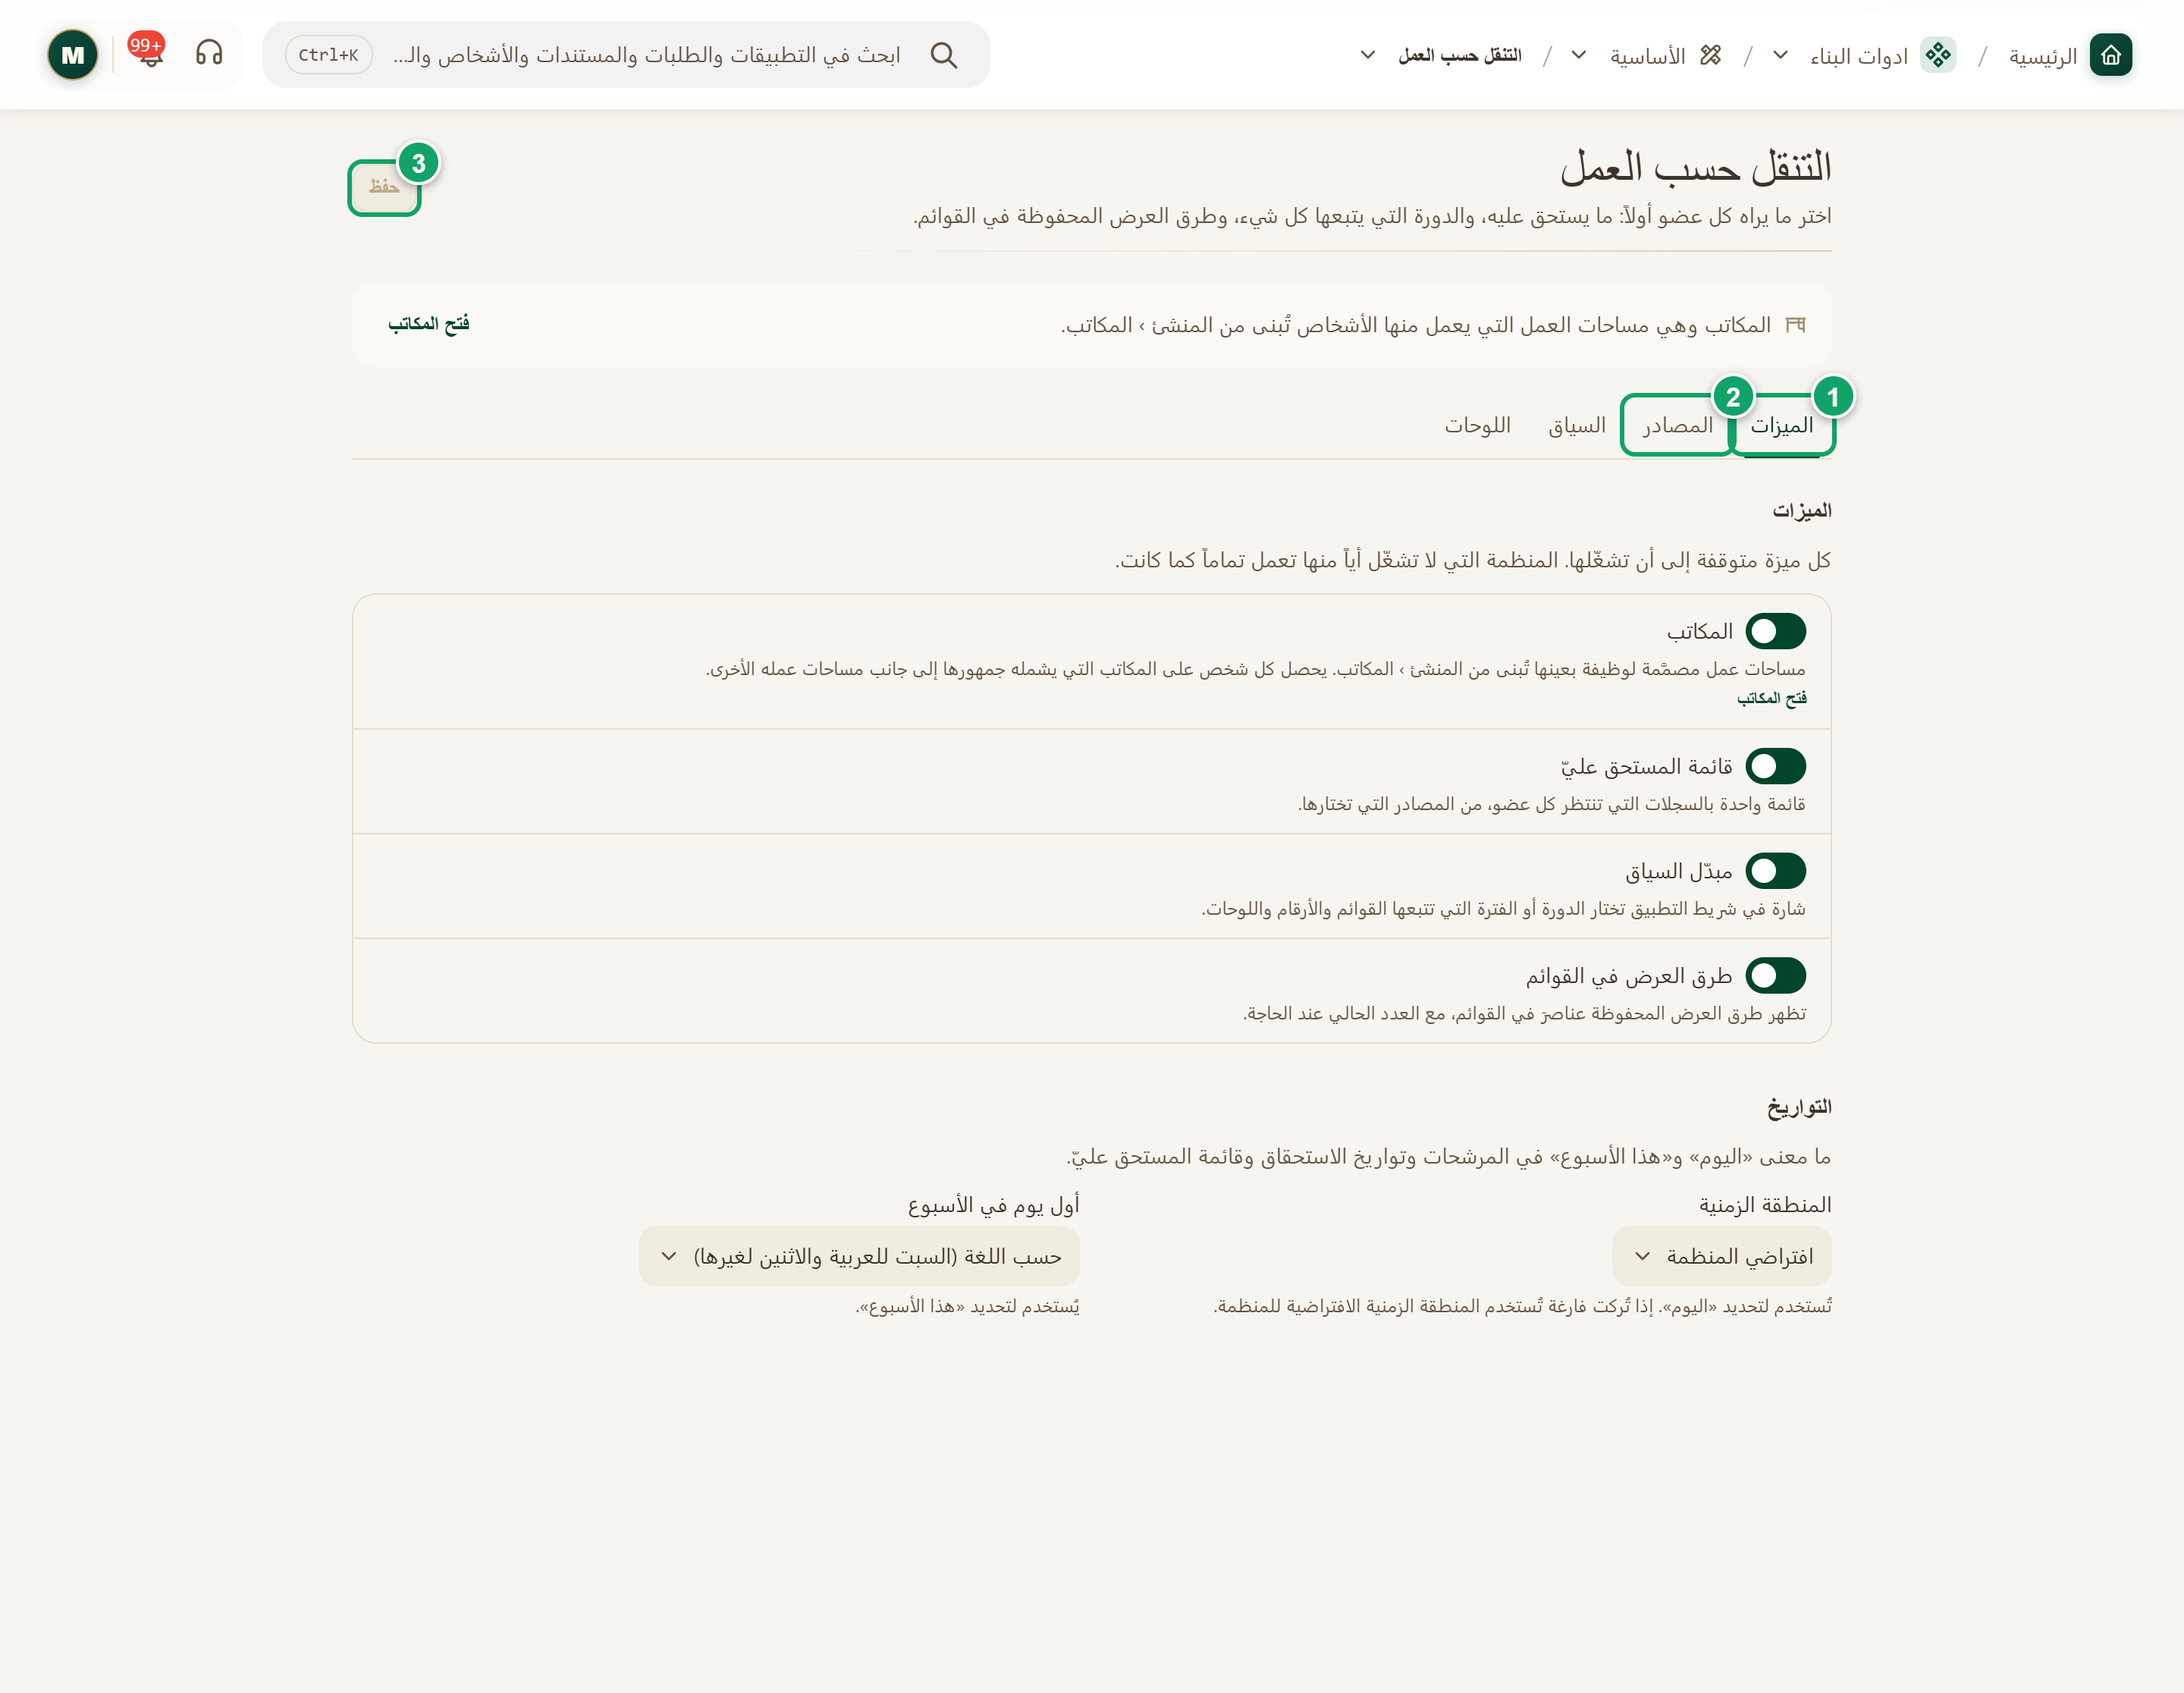
\includegraphics[width=0.95\linewidth,height=0.72\textheight,keepaspectratio]{figures/screens/ch06-work-navigation-ar.png}
\caption{صفحة «التنقل حسب العمل»}
\label{fig:builder-work-navigation-screen}
\shotnote{تعرض الصورة تبويب «الميزات» في مؤسسة الاختبار، وقد شُغّلت فيه الميزات الأربع، أما في مؤسسة لم تضبط الصفحة فتبدأ كلها متوقفة. وتُحفظ التبويبات الأربعة معاً بزر واحد، لذلك راجع ما غيّرته فيها قبل الحفظ. ① «الميزات»: التبويب الذي تشغّل منه «المكاتب» و«قائمة المستحق عليّ» وغيرهما. ② مفتاح «قائمة المستحق عليّ»: يشغّل القائمة التي تجمع ما ينتظر العضو. ③ «المصادر»: يحدد ما يغذّي هذه القائمة. ④ «حفظ»: يحفظ الإعدادات، ويبقى معطلاً حتى تغيّر شيئاً.}
\end{figure}

\begin{table}[H]
\centering
\caption{تبويب «الميزات»}
\label{tab:builder-work-navigation-data}
\begin{tabularx}{\linewidth}{R{3.6cm} Y}
\rcHeaderRow
\thh{الإعداد} & \thh{ماذا يفعل؟}\\
المكاتب & يشغّل المكاتب، وهي مساحات عمل مصمَّمة لوظيفة بعينها. وتُبنى المكاتب في صفحة مستقلة تفتحها من رابط «فتح المكاتب».\\
قائمة المستحق عليّ & يجمع في قائمة واحدة السجلات التي تنتظر كل عضو، من المصادر التي تضيفها في تبويب «المصادر».\\
مبدّل السياق & يُظهر شريحة في شريط التطبيق يختار منها العضو الدورة أو الفترة التي تتبعها القوائم والأرقام واللوحات.\\
طرق العرض في القوائم & يتيح وضع طرق العرض المحفوظة عناصرَ في القوائم، مع عددها الحالي عند الحاجة.\\
التواريخ & «المنطقة الزمنية» التي يُحسب بها «اليوم»، و«أول يوم في الأسبوع» الذي يُحسب به «هذا الأسبوع»، في التصفية وتواريخ الاستحقاق وقائمة المستحق.\\
\end{tabularx}
\end{table}

\begin{table}[H]
\centering
\caption{بقية التبويبات}
\label{tab:builder-work-navigation-tabs}
\begin{tabularx}{\linewidth}{R{3.6cm} Y}
\rcHeaderRow
\thh{التبويب} & \thh{ماذا تحدد فيه؟}\\
المصادر & ما يغذّي قائمة «المستحق عليّ». ويشرحه قسم «مصادر قائمة المستحق عليّ».\\
السياق & نوع السجلات الذي تتبعه التطبيقات والأقسام المختارة. ويشرحه قسم «السياق».\\
اللوحات & نطاق بيانات اللوحات الجديدة، والانتقال باللوحات القديمة إلى صلاحيات المشاهد. ويشرحه قسم «نطاق بيانات اللوحات».\\
\end{tabularx}
\end{table}

\begin{figure}[H]
\centering
\begin{tikzpicture}[node distance=0.5cm]
\node[entity] (member) {\RL{العضو}};
\node[entityOpt,below right=0.7cm and 0.3cm of member] (desk) {\RL{المكاتب}};
\node[entityOpt,below left=0.7cm and 0.3cm of member] (due) {\RL{المستحق عليّ}};
\draw[dependsOnOpt] (member.south) -- ++(0,-0.3) -| (desk.north);
\draw[dependsOnOpt] (member.south) -- ++(0,-0.3) -| (due.north);
\end{tikzpicture}
\rclegend
\caption{ما يراه العضو أولاً}
\label{fig:builder-work-navigation-model}
\shotnote{يوضّح الشكل أن هذه الصفحة لا تُنشئ بيانات جديدة، بل تقرّب العمل الموجود من العضو: مكاتب تناسب وظيفته، وقائمة تجمع ما يستحق عليه من أنواع سجلات مختلفة. وكلاهما اختياري، لذلك فعّل ميزة واحدة وجرّبها قبل تفعيل غيرها.}
\end{figure}

\subsection{خطوات العمل والتحقق}
\begin{enumerate}
\item افتح «التنقل حسب العمل»، وشغّل في «الميزات» الميزة التي تحتاجها المؤسسة.
\item اختر «المنطقة الزمنية» و«أول يوم في الأسبوع» إذا كانت القيم الافتراضية لا تناسب المؤسسة.
\item إذا شغّلت «قائمة المستحق عليّ»، فانتقل إلى «المصادر» وأضف مصدراً واحداً على الأقل.
\item اضغط «حفظ» في رأس الصفحة، أو «تجاهل التغييرات» إذا أردت التراجع عن كل ما لم تحفظه.
\end{enumerate}

\textbf{تحقق ومعالجة المشكلة:} يجب أن تظهر رسالة «تم حفظ التنقل حسب العمل»، وأن يصبح زر «حفظ» معطلاً حتى تغيّر شيئاً آخر. فإذا ظهر تحت «قائمة المستحق عليّ» التنبيه «أضف مصدراً واحداً على الأقل في تبويب المصادر وإلا بقيت القائمة فارغة.»، فأضف مصدراً قبل أن تخبر الأعضاء بالميزة. وإذا ظهرت «إعدادات تحتاج إلى مراجعة» أو رسالة تعارض في الحفظ، فاتبع قسم «إعدادات تحتاج إلى مراجعة».

\clearpage
\section{مصادر قائمة المستحق عليّ}
\label{sec:builder-feature-work-navigation-sources}

قائمة «المستحق عليّ» فارغة في البداية، ولا يظهر فيها إلا ما تحدده المصادر. والمصدر قاعدة تقول: اعرض للعضو هذه السجلات لأنها تنتظره. وقد تكون السجلات التي يستطيع العضو تنفيذ انتقال عليها الآن، أو السجلات المسندة إليه في حقل عضو، أو قائمة مضمّنة في النظام مثل الموافقات.

ويضيف كل مصدر سجلاته إلى قوائم كل الأعضاء الذين تنطبق عليهم شروطه، ويمكن حصره في أدوار معينة. ولا يعطي المصدر أحداً صلاحية جديدة، فالعضو لا يرى إلا السجلات التي يستطيع فتحها.

\textbf{المسار ومن يستخدمه:} «ادوات البناء» ← «الأساسية» ← «التنقل حسب العمل» ← «المصادر». يستخدمه مالك المؤسسة ومسؤولها بعد تشغيل «قائمة المستحق عليّ».

\begin{rcnote}[مثال: شركة الأفق]
يضيف مسؤول النظام مصدراً من نوع «انتقالات أستطيع تنفيذها» باسم «زيارات بانتظار القرار»، ويختار «طلبات الزيارة» وحقل حالتها وانتقال الاعتماد. فتظهر الطلبات في قائمة سارة الخطيب لأنها تملك صلاحية الاعتماد، ولا تظهر لعمر حداد. ويضيف المصدر من ② ويحفظ من ③، ثم يتحقق منه من ④.
\end{rcnote}

\begin{figure}[H]
\centering
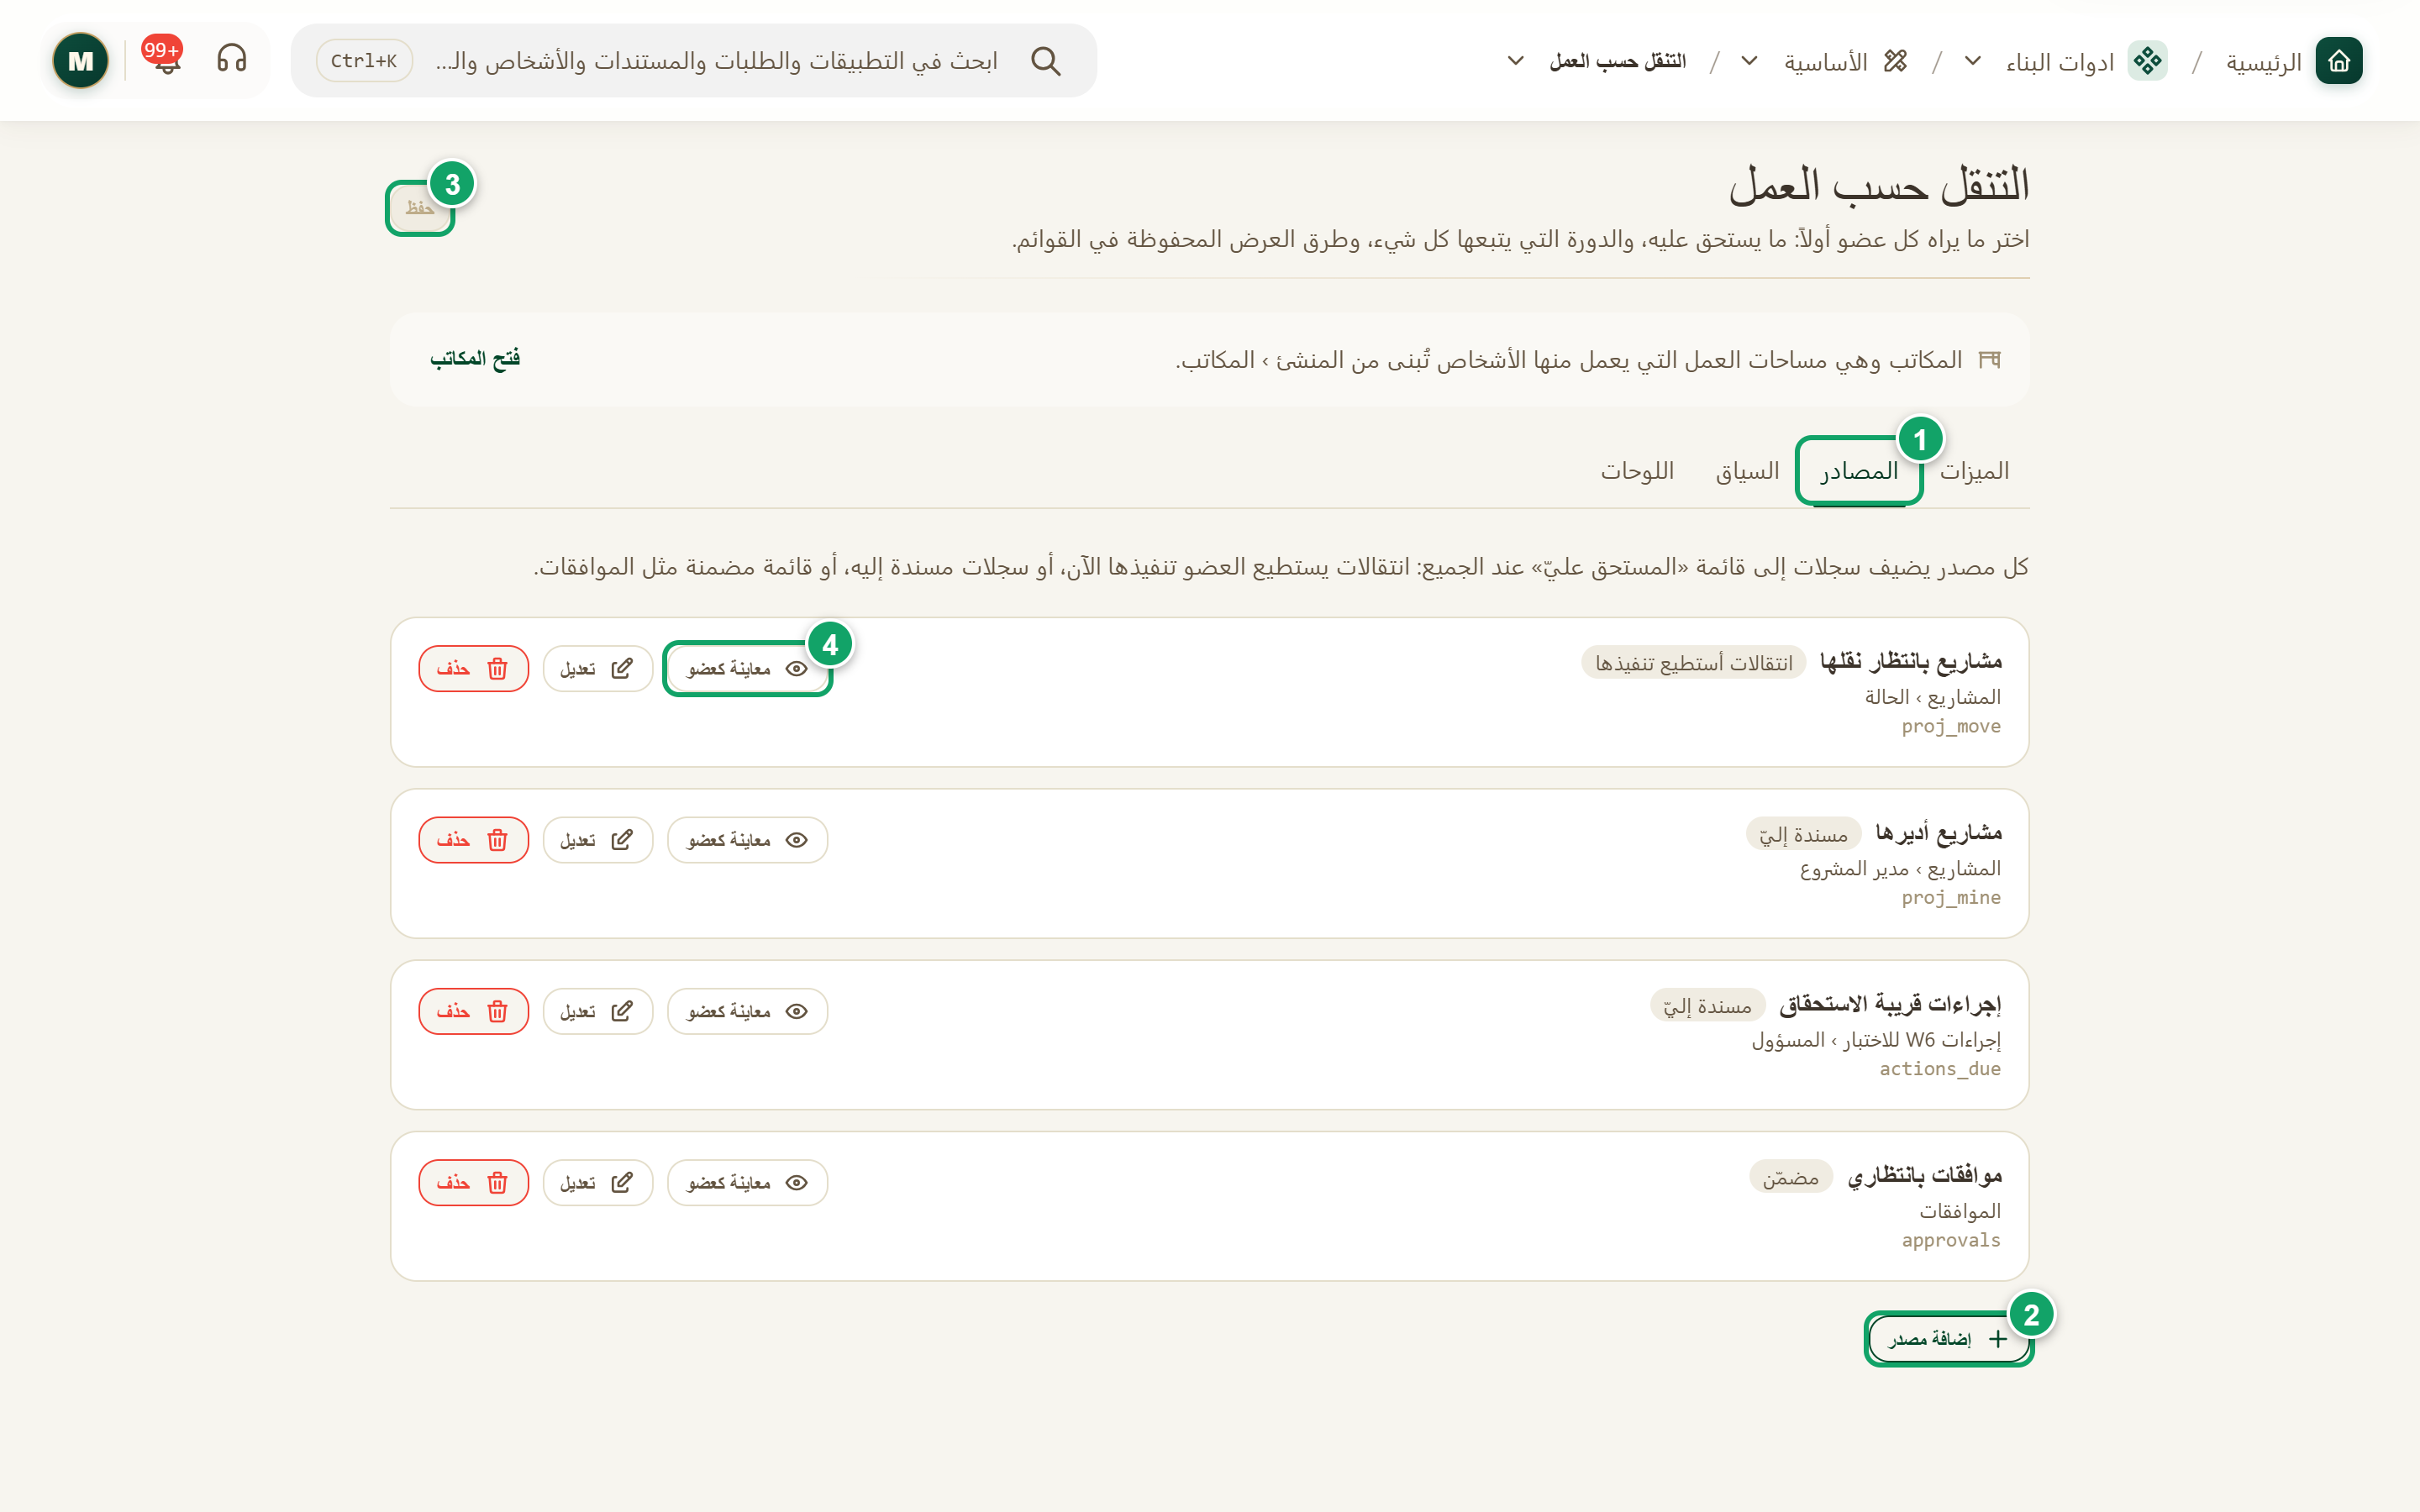
\includegraphics[width=0.95\linewidth,height=0.72\textheight,keepaspectratio]{figures/screens/ch06-wn-sources-ar.png}
\caption{تبويب «المصادر»}
\label{fig:builder-work-navigation-sources-screen}
\shotnote{تعرض الصورة تبويب «المصادر» في مؤسسة الاختبار، وفيه أربعة مصادر من الأنواع الثلاثة، يحمل كل منها شارة نوعه ونوع السجل الذي يقرؤه ومفتاحه. ويفيدك ذلك في مقارنة المصادر الموجودة قبل أن تضيف مصدراً جديداً. ① «المصادر»: التبويب الذي يعرض المصادر. ② «إضافة مصدر»: يفتح نافذة المصدر الجديد. ③ «حفظ»: يحفظ المصادر مع بقية إعدادات الصفحة. ④ «معاينة كعضو»: يعرض عدد السجلات وأمثلة منها بعد الحفظ.}
\end{figure}

\begin{table}[H]
\centering
\caption{أنواع المصادر}
\label{tab:builder-work-navigation-sources-kinds}
\begin{tabularx}{\linewidth}{R{3.6cm} Y}
\rcHeaderRow
\thh{النوع} & \thh{ما يجلبه وما تحدده}\\
انتقالات أستطيع تنفيذها & سجلات يستطيع العضو تنفيذ انتقال عليها الآن، مثل الاعتماد أو المراجعة. تختار «نوع السجل» و«حقل الحالة» و«الانتقالات التي تُعد عملاً»، وإذا تركتها فارغة شملت كل الانتقالات عدا التعديل العادي.\\
مسندة إليّ & سجلات يذكر فيها أحد «حقول العضو» هذا العضو. ويمكنك تحديد «ما الحالات المفتوحة»: «أي حالة» أو «حسب الفئة» أو «حالات محددة»، وتحديد فترة بحقلي «يبدأ في (حقل)» و«ينتهي في (حقل)».\\
مضمّن & قائمة جاهزة تختارها من «القائمة المضمنة»، مثل «الموافقات» و«موافقات الإجراءات» و«المهام» و«طلبات المهام» و«الدورات».\\
\end{tabularx}
\end{table}

\begin{table}[H]
\centering
\caption{إعدادات مشتركة في نافذة المصدر}
\label{tab:builder-work-navigation-sources-common}
\begin{tabularx}{\linewidth}{R{3.6cm} Y}
\rcHeaderRow
\thh{الإعداد} & \thh{ما يحدده}\\
ماذا تعني الصفوف للشخص & «عمل للإنجاز» أو «متابعة» أو «بانتظار الآخرين». وللسجلات المسندة التي تنتظر الآخرين حقل «متأخر بعد (بالأيام)».\\
الاسم والمفتاح & «الاسم» يظهر للأعضاء، و«المفتاح» معرّف بحروف لاتينية وأرقام وشرطات سفلية لا يتغير بعد إضافة المصدر.\\
الاستحقاق & «حقل تاريخ الاستحقاق»، و«يستحق خلال (أيام)» لعرض المتأخر وما يستحق قريباً.\\
عرض الصف & «عنوان الصف» و«العنوان الفرعي للصف»، و«فتح هذا السجل المرتبط» ليفتح الصف سجلاً آخر يشير إليه الحقل.\\
الأدوار والأولوية & «الأدوار التي تراه»، وإذا تُركت فارغة رآه كل من يستطيع فتح السجلات؛ و«الأولوية»، والمصدر ذو الرقم الأصغر يظهر أولاً.\\
مرشحات إضافية (متقدم) & شروط إضافية بصيغة \en{JSON} لمن يحتاج تصفية أدق.\\
\end{tabularx}
\end{table}

\begin{figure}[H]
\centering
\begin{tikzpicture}[node distance=0.5cm]
\node[stepBox] (a) {\RL{إضافة مصدر}};
\node[stepBox,below=of a] (b) {\RL{النوع ومعنى الصفوف}};
\node[stepBox,below=of b] (c) {\RL{نوع السجل والحقول}};
\node[stepBox,below=of c] (d) {\RL{الأدوار والأولوية}};
\node[stepBox,below=of d] (e) {\RL{حفظ الصفحة}};
\node[stepBox,below=of e] (f) {\RL{معاينة كعضو}};
\draw[flowsTo] (a) -- (b);
\draw[flowsTo] (b) -- (c);
\draw[flowsTo] (c) -- (d);
\draw[flowsTo] (d) -- (e);
\draw[flowsTo] (e) -- (f);
\end{tikzpicture}
\rclegend
\caption{إضافة مصدر وتجربته}
\label{fig:builder-work-navigation-sources-flow}
\shotnote{يضع المخطط المعاينة بعد الحفظ لأنها تقرأ الإعدادات المحفوظة فقط، فلا تعرض شيئاً لمصدر لم يُحفظ بعد. أما زر النافذة فيضيف المصدر إلى المسودة، ولذلك تبقى خطوة «حفظ» في رأس الصفحة ضرورية.}
\end{figure}

\subsection{خطوات العمل والتحقق}
\begin{enumerate}
\item افتح «التنقل حسب العمل»، ثم تبويب «المصادر»، واضغط «إضافة مصدر».
\item اختر «النوع» و«ماذا تعني الصفوف للشخص»، واكتب «الاسم» و«المفتاح».
\item اختر «نوع السجل» والحقول التي يطلبها النوع، وحدد «الأدوار التي تراه» عند الحاجة.
\item اضغط «إضافة مصدر» في النافذة، ثم «حفظ» في رأس الصفحة.
\item اضغط «معاينة كعضو» في صف المصدر لترى عدد السجلات وأمثلة منها بصلاحياتك أنت.
\end{enumerate}

\textbf{تحقق ومعالجة المشكلة:} يجب أن يظهر المصدر في القائمة، وأن تعرض المعاينة عدداً بعد الحفظ. فإذا بقي زر النافذة معطلاً، فاقرأ الرسائل أسفلها، مثل «اختر نوع سجل.» أو «يستخدم مصدر آخر هذا المفتاح.». وإذا قالت المعاينة «لا تحمل أياً من أدوار هذا المصدر، فلا شيء تعاينه بصلاحياتك.»، فالمصدر صحيح لكنه مخصص لأدوار لا تملكها. ويتسع التبويب لعشرين مصدراً على الأكثر.

\clearpage
\section{السياق}
\label{sec:builder-feature-work-navigation-context}

السياق نوع سجلات، مثل الدورة أو السنة، تتبعه القوائم والأرقام واللوحات في تطبيقات وأقسام تختارها. فيختار العضو قيمة السياق مرة واحدة من شريحة في شريط التطبيق، ثم تعرض له كل صفحات تلك التطبيقات ما يخص هذه القيمة فقط. ويوفّر ذلك على العضو تكرار التصفية نفسها في كل قائمة.

ولا تظهر الشريحة للأعضاء إلا بعد تشغيل «مبدّل السياق» في «الميزات». ويمكن تعريف ثلاثة سياقات على الأكثر.

\textbf{المسار ومن يستخدمه:} «ادوات البناء» ← «الأساسية» ← «التنقل حسب العمل» ← «السياق». يستخدمه مالك المؤسسة ومسؤولها عندما يُنظَّم العمل بدورات أو فترات.

\begin{rcnote}[مثال: شركة الأفق]
تنظّم الأفق زياراتها في دورات ربع سنوية. فيضيف مسؤول النظام سياقاً من نوع سجلات الدورات، ويجعل تطبيق «خدمات الفروع» يتبعه، ويختار علاقة «طلبات الزيارة» بالدورة. فإذا اختارت سارة الخطيب الدورة الحالية، لا ترى إلا طلباتها. ويختار نوع السجل من ② والتطبيق من ④.
\end{rcnote}

\begin{figure}[H]
\centering
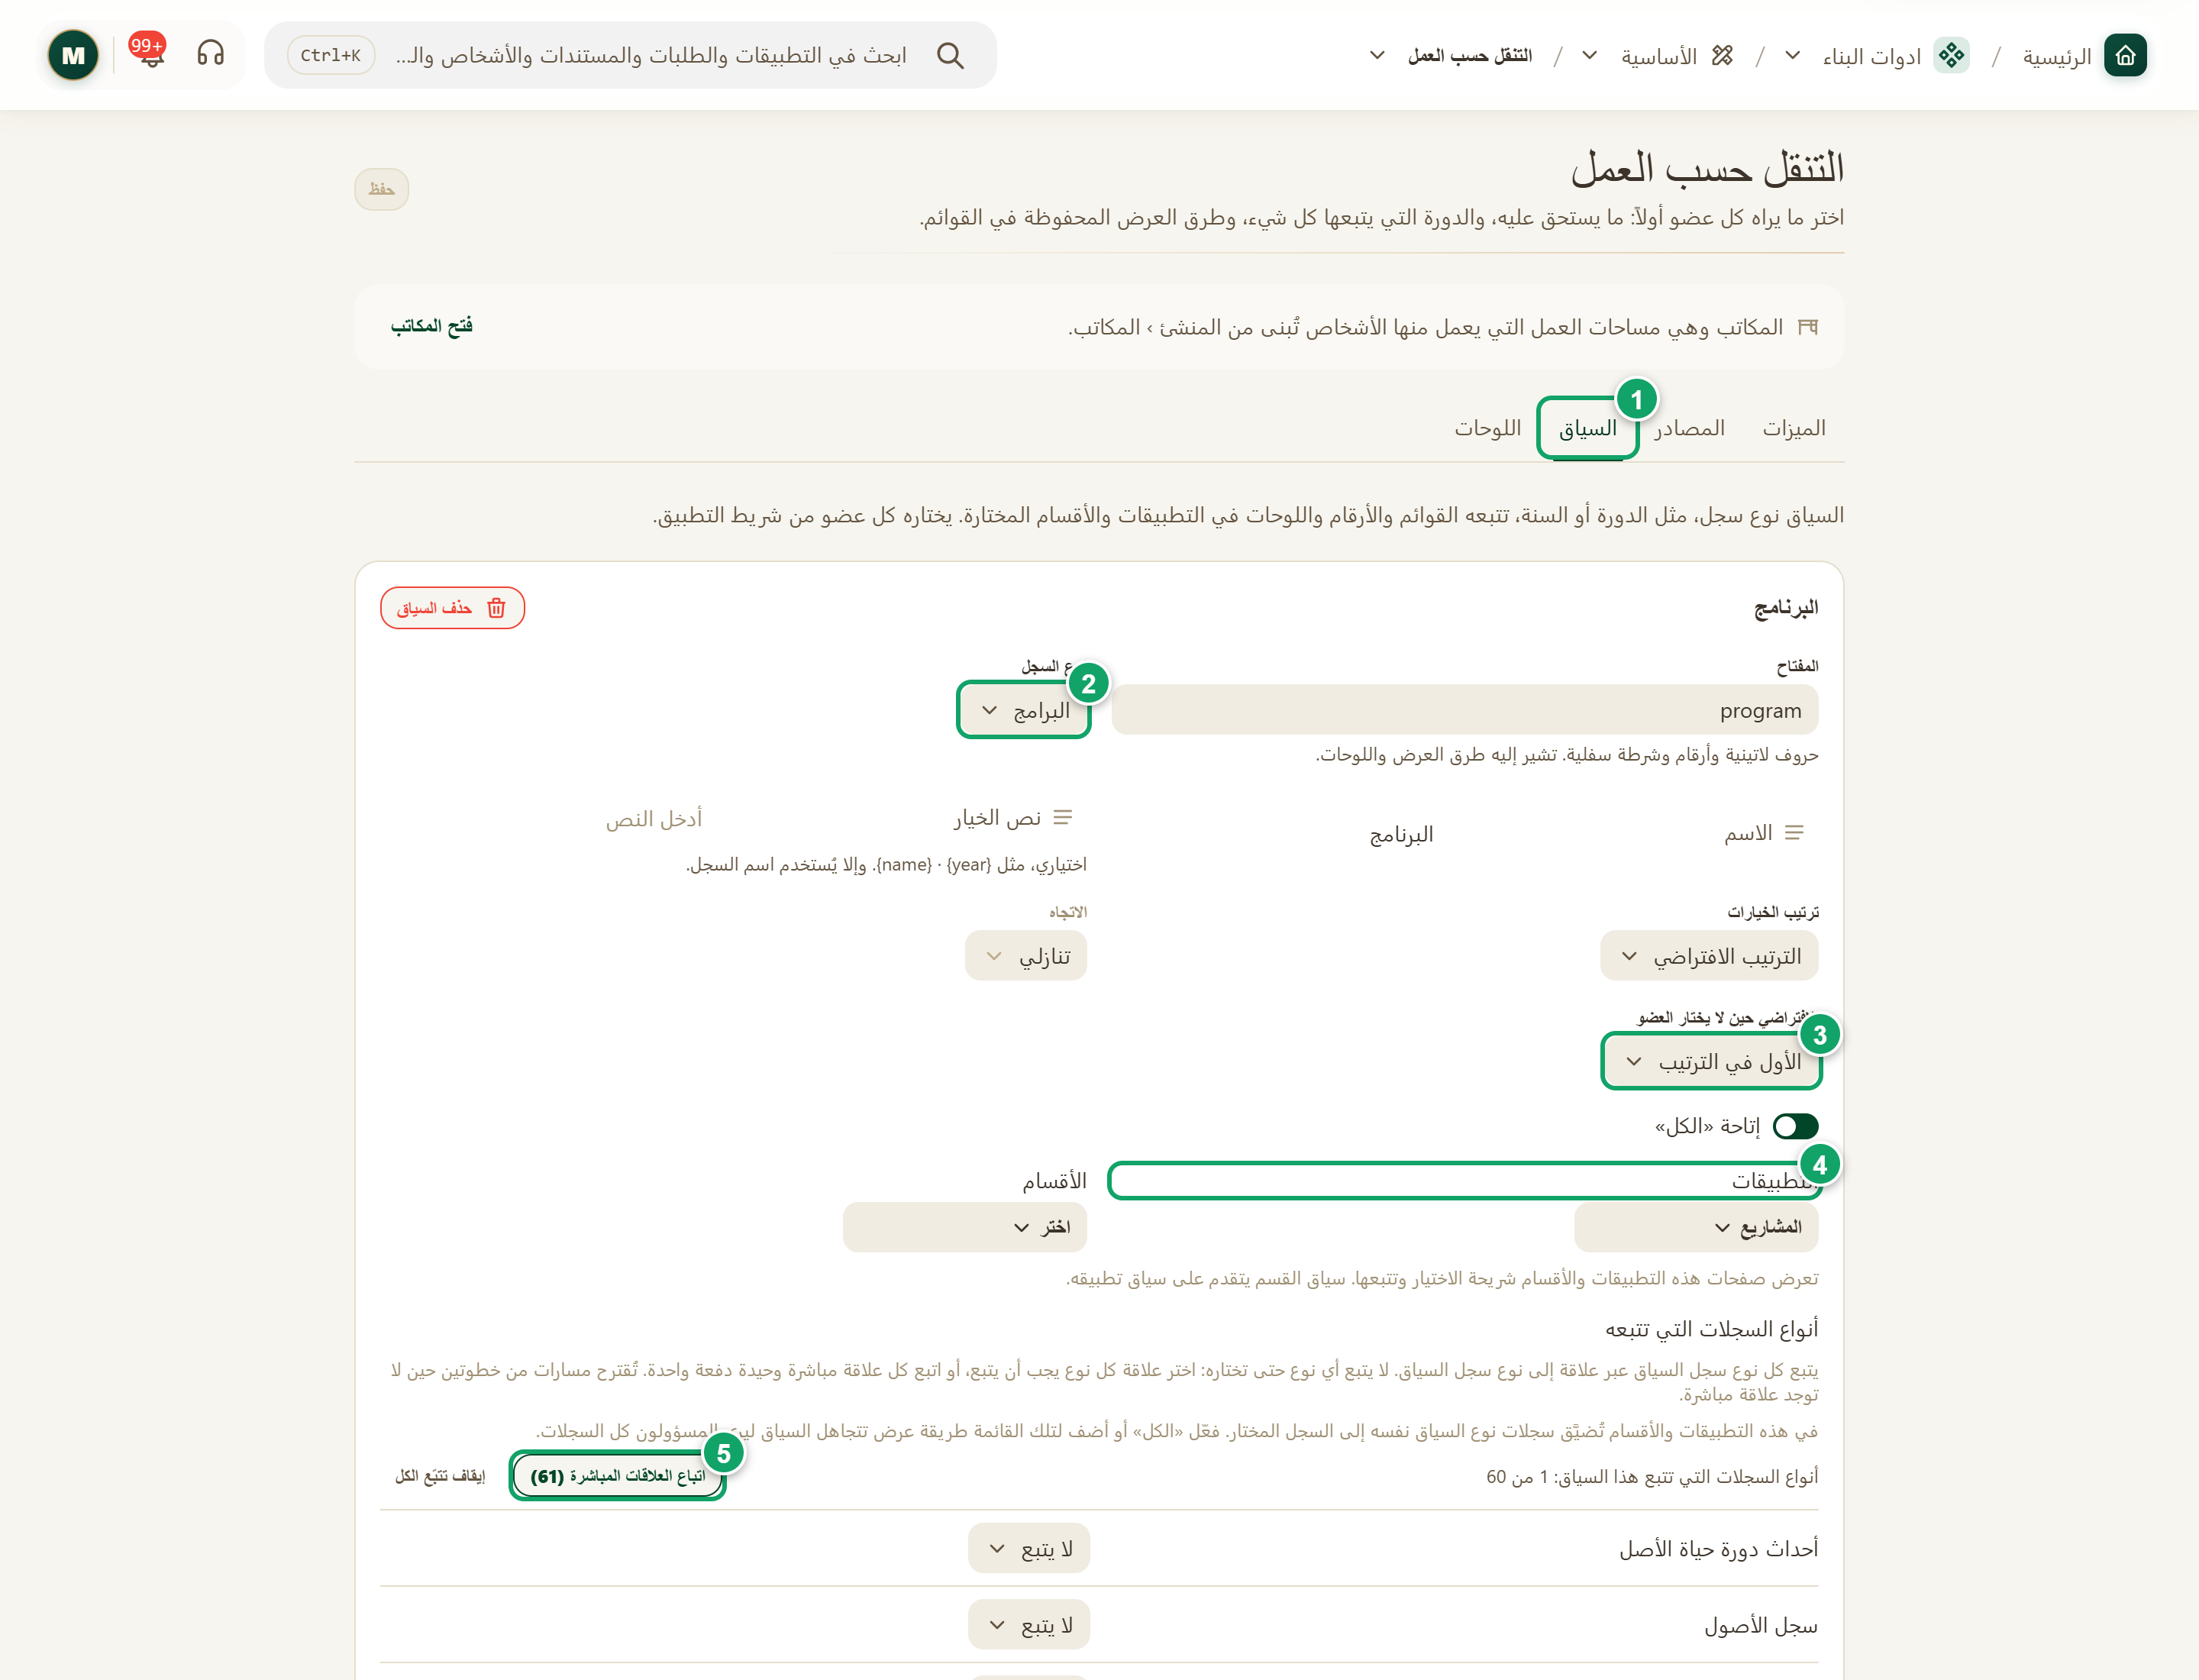
\includegraphics[width=0.95\linewidth,height=0.72\textheight,keepaspectratio]{figures/screens/ch06-wn-context-ar.png}
\caption{تبويب «السياق»}
\label{fig:builder-work-navigation-context-screen}
\shotnote{تعرض الصورة تبويب «السياق» في مؤسسة الاختبار، وفيه سياق باسم «البرنامج» مبني على نوع السجلات «البرامج» ويتبعه تطبيق «المشاريع». ويظهر في أسفله جدول «أنواع السجلات التي تتبعه»، وأغلب أنواعه على «لا يتبع» لأن التتبع لا يبدأ حتى تختاره. ① «السياق»: التبويب الذي تضبط فيه السياقات. ② «نوع السجل»: نوع الدورات أو السنوات الذي يُبنى عليه السياق. ③ «الافتراضي حين لا يختار العضو»: القيمة المعروضة قبل أن يختار العضو. ④ «التطبيقات»: الأماكن التي تعرض الشريحة وتتبعها، وبجانبها «الأقسام». ⑤ «اتباع العلاقات المباشرة»: يختار كل علاقة مباشرة وحيدة دفعة واحدة.}
\end{figure}

\begin{table}[H]
\centering
\caption{إعدادات السياق}
\label{tab:builder-work-navigation-context-fields}
\begin{tabularx}{\linewidth}{R{3.6cm} Y}
\rcHeaderRow
\thh{الإعداد} & \thh{ما يحدده}\\
المفتاح ونوع السجل والاسم & «المفتاح» معرّف تشير إليه طرق العرض واللوحات، و«نوع السجل» هو نوع الدورات أو السنوات، و«الاسم» هو ما يراه العضو.\\
نص الخيار & صيغة اختيارية لنص كل خيار في الشريحة. وإذا تُرك فارغاً يُستخدم اسم السجل.\\
ترتيب الخيارات والاتجاه & الحقل الذي تُرتَّب به الخيارات، و«تصاعدي» أو «تنازلي».\\
الافتراضي حين لا يختار العضو & «الأول في الترتيب»، أو «الأول في حالة معينة» مع «حقل الحالة» و«الحالات»، أو «لا شيء (عرض الكل)».\\
إتاحة «الكل» & يضيف إلى الشريحة خياراً يعرض كل السجلات دون تضييق.\\
التطبيقات والأقسام & الأماكن التي تعرض الشريحة وتتبعها. وسياق القسم يتقدم على سياق تطبيقه.\\
أنواع السجلات التي تتبعه & لكل نوع سجلات تختار في «يتبع عبر» العلاقة التي يتبع بها السياق، أو تختار «لا يتبع». ويختار زر «اتباع العلاقات المباشرة» كل علاقة مباشرة وحيدة دفعة واحدة.\\
\end{tabularx}
\end{table}

\begin{rcwarn}[لا يتبع أي نوع حتى تختاره]
إضافة التطبيق إلى السياق لا تكفي وحدها؛ فلا يتضيق نوع سجلات حتى تختار له علاقة في «أنواع السجلات التي تتبعه». ثم إن سجلات نوع السياق نفسه تتضيق إلى القيمة المختارة في تلك الأماكن، لذلك فعّل «الكل» حتى يستطيع المسؤولون رؤية كل السجلات.
\end{rcwarn}

\begin{figure}[H]
\centering
\begin{tikzpicture}[node distance=0.5cm]
\node[stepBox] (a) {\RL{تشغيل مبدّل السياق}};
\node[stepBox,below=of a] (b) {\RL{إضافة سياق}};
\node[stepBox,below=of b] (c) {\RL{نوع السجل والافتراضي}};
\node[stepBox,below=of c] (d) {\RL{التطبيقات والأقسام}};
\node[stepBox,below=of d] (e) {\RL{الأنواع التي تتبعه}};
\node[stepBox,below=of e] (f) {\RL{حفظ}};
\draw[flowsTo] (a) -- (b);
\draw[flowsTo] (b) -- (c);
\draw[flowsTo] (c) -- (d);
\draw[flowsTo] (d) -- (e);
\draw[flowsTo] (e) -- (f);
\end{tikzpicture}
\rclegend
\caption{ضبط سياق مشترك}
\label{fig:builder-work-navigation-context-flow}
\shotnote{يبدأ المخطط بتشغيل الميزة لأن الشريحة لا تظهر للأعضاء من دونها، حتى لو كان السياق مضبوطاً. ويضع اختيار الأنواع التابعة بعد الأماكن، لأن المكان يحدد أين تظهر الشريحة، أما العلاقة فتحدد أي السجلات تتضيق فعلاً.}
\end{figure}

\subsection{خطوات العمل والتحقق}
\begin{enumerate}
\item شغّل «مبدّل السياق» في تبويب «الميزات».
\item افتح تبويب «السياق» واضغط «إضافة سياق»، ثم اكتب «المفتاح» واختر «نوع السجل» واكتب «الاسم».
\item اختر «الافتراضي حين لا يختار العضو»، وفعّل «إتاحة «الكل»» عند الحاجة.
\item اختر «التطبيقات» و«الأقسام» التي تتبعه، ثم اختر لكل نوع سجلات العلاقة التي يتبع عبرها.
\item اضغط «حفظ» في رأس الصفحة.
\end{enumerate}

\textbf{تحقق ومعالجة المشكلة:} بعد الحفظ وإعادة تحميل الصفحة، تظهر الشريحة في شريط التطبيقات المختارة، وتتضيق قوائمها عند اختيار قيمة. فإذا لم تتضيق قائمة ما، فارجع إلى «أنواع السجلات التي تتبعه» وتأكد من أن نوعها لا يحمل «لا يتبع». وإذا ظهر بجانب تطبيق «يتبع «…» مسبقاً»، فهو تابع لسياق آخر، فأزله من ذلك السياق أولاً.

\clearpage
\section{نطاق بيانات اللوحات}
\label{sec:builder-feature-work-navigation-dashboards}

تعرض لوحة المعلومات أرقاماً ورسوماً محسوبة من السجلات. ويحدد «نطاق البيانات» السجلات التي تُحسب منها: إما «بصلاحيات المشاهد»، فيرى كل شخص أرقاماً من السجلات التي يحق له رؤيتها فقط، وإما «بيانات المنظمة كاملة»، فيرى كل من يفتح اللوحة أرقام كل السجلات.

ويضبط هذا التبويب أمرين: النطاق الذي تُنشأ به اللوحات الجديدة، وقائمة اللوحات الحالية التي ما زالت تعرض بيانات المؤسسة كاملة، مع إمكانية تحويلها إلى صلاحيات المشاهد.

\textbf{المسار ومن يستخدمه:} «ادوات البناء» ← «الأساسية» ← «التنقل حسب العمل» ← «اللوحات». ولا يرى قائمة اللوحات إلا مالكو المؤسسة ومسؤولوها.

\begin{rcnote}[مثال: شركة الأفق]
يجد مسؤول النظام في القائمة لوحة الزيارات التي تعرض أرقام الفرعين لكل من يفتحها. فيحوّلها إلى صلاحيات المشاهد، فيرى عمر حداد أرقام طلباته فقط، بينما ترى سارة الخطيب ما تسمح به صلاحياتها. ويحوّل اللوحة من ④.
\end{rcnote}

\begin{figure}[H]
\centering
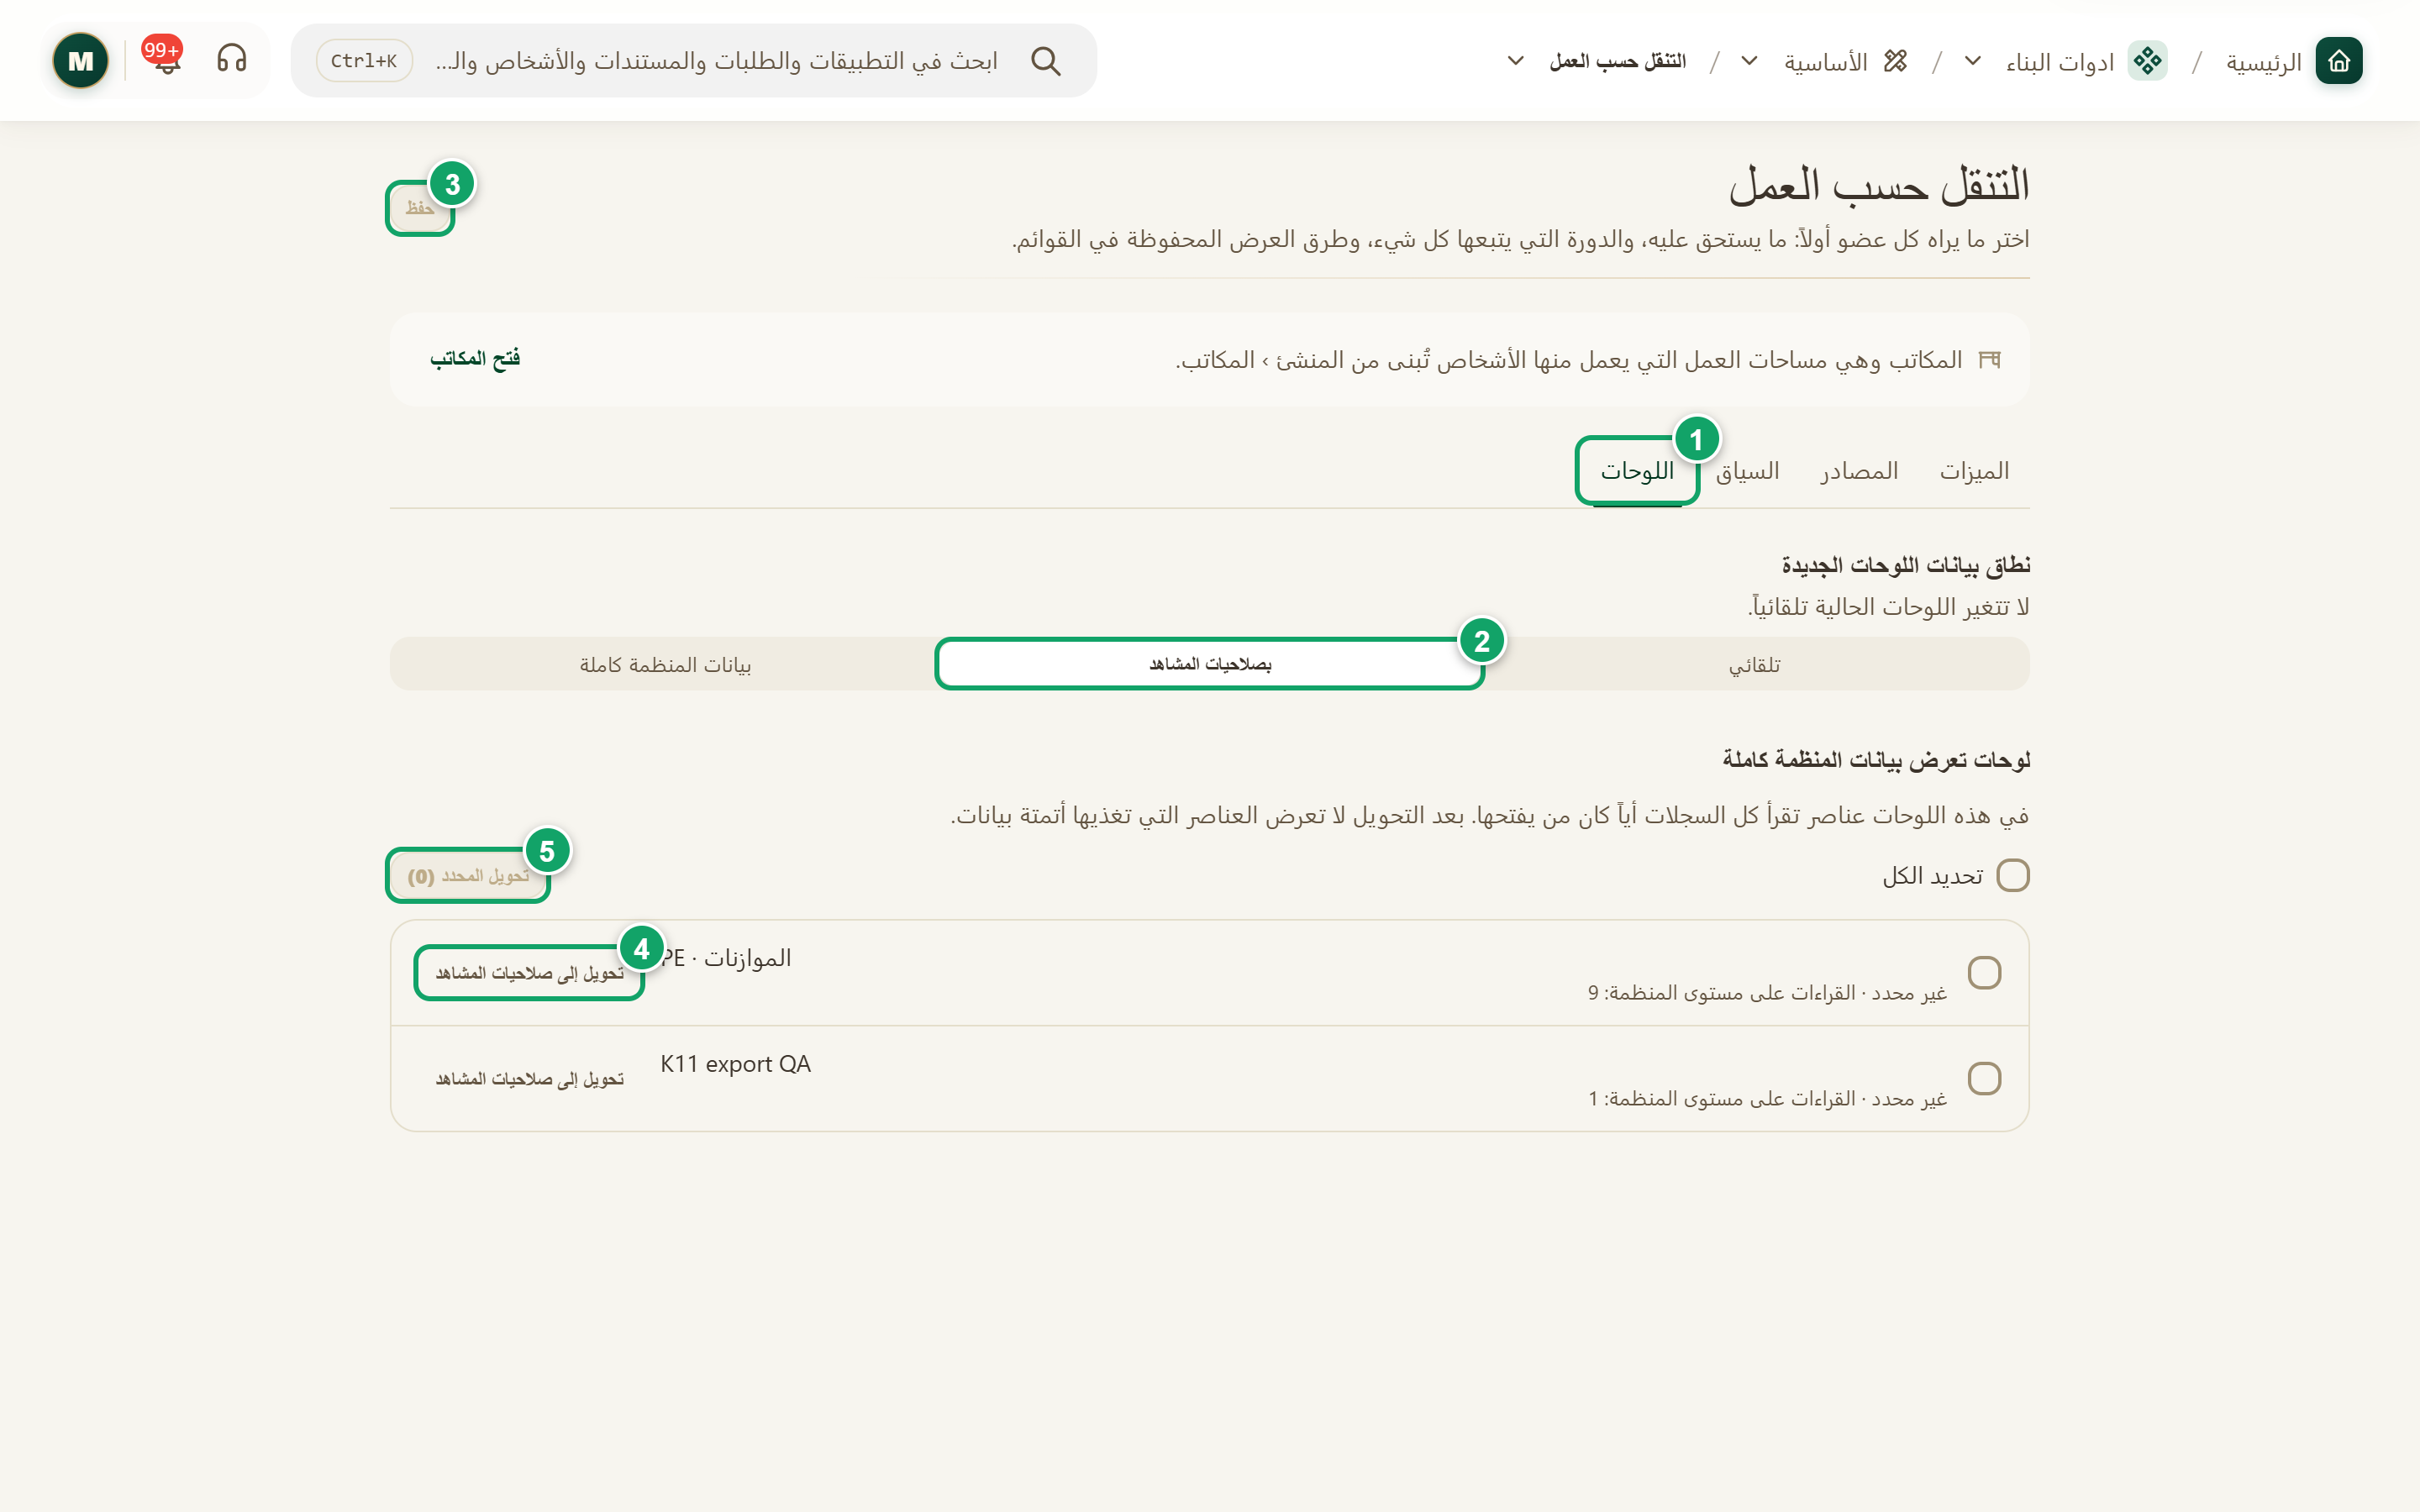
\includegraphics[width=0.95\linewidth,height=0.72\textheight,keepaspectratio]{figures/screens/ch06-wn-dashboards-ar.png}
\caption{تبويب «اللوحات»}
\label{fig:builder-work-navigation-dashboards-screen}
\shotnote{تعرض الصورة تبويب «اللوحات» في مؤسسة الاختبار، ونطاق اللوحات الجديدة فيه «بصلاحيات المشاهد»، بينما تبقى في القائمة لوحتان تقرآن بيانات المؤسسة كاملة مع عدد هذه القراءات. ويبيّن ذلك أن اختيار النطاق لا يغيّر اللوحات الحالية، وأن تحويلها خطوة مستقلة تُنفَّذ فوراً. ① «اللوحات»: التبويب. ② «بصلاحيات المشاهد»: نطاق اللوحات الجديدة. ③ «حفظ»: يحفظ اختيار النطاق. ④ «تحويل إلى صلاحيات المشاهد»: يحوّل لوحة واحدة. ⑤ «تحويل المحدد»: يحوّل كل اللوحات التي حددتها.}
\end{figure}

\begin{table}[H]
\centering
\caption{محتوى تبويب «اللوحات»}
\label{tab:builder-work-navigation-dashboards-parts}
\begin{tabularx}{\linewidth}{R{3.6cm} Y}
\rcHeaderRow
\thh{الجزء} & \thh{ما يفعله}\\
نطاق بيانات اللوحات الجديدة & «تلقائي» أو «بصلاحيات المشاهد» أو «بيانات المنظمة كاملة». والتلقائي يعني صلاحيات المشاهد ما دامت إحدى ميزات التنقل حسب العمل مفعّلة. ولا تتغير اللوحات الحالية بهذا الاختيار.\\
لوحات تعرض بيانات المنظمة كاملة & قائمة باللوحات التي فيها عناصر تقرأ كل السجلات أياً كان من يفتحها، مع عدد هذه القراءات لكل لوحة.\\
تحويل إلى صلاحيات المشاهد & يحوّل لوحة واحدة، أو يحوّل «تحويل المحدد» كل اللوحات التي حددتها. ويُنفَّذ التحويل فوراً دون انتظار «حفظ».\\
\end{tabularx}
\end{table}

\begin{rcwarn}[قبل التحويل]
بعد التحويل لا تعرض العناصر التي تغذيها أتمتة أي بيانات، لأن الأتمتة لا تعمل بصلاحيات المشاهد. لذلك راجع اللوحة بعد تحويلها، وأعد بناء هذه العناصر إن احتجت إليها.
\end{rcwarn}

\begin{figure}[H]
\centering
\begin{tikzpicture}[node distance=0.5cm]
\node[stepBox] (a) {\RL{اختيار نطاق اللوحات الجديدة}};
\node[stepBox,below=of a] (b) {\RL{حفظ}};
\node[stepBox,below=of b] (c) {\RL{مراجعة قائمة اللوحات}};
\node[stepBox,below=of c] (d) {\RL{تحويل إلى صلاحيات المشاهد}};
\node[stepBox,below=of d] (e) {\RL{فتح اللوحة ومراجعتها}};
\draw[flowsTo] (a) -- (b);
\draw[flowsTo] (b) -- (c);
\draw[flowsTo] (c) -- (d);
\draw[flowsTo] (d) -- (e);
\end{tikzpicture}
\rclegend
\caption{ضبط نطاق بيانات اللوحات}
\label{fig:builder-work-navigation-dashboards-flow}
\shotnote{يفصل المخطط بين إجراءين يُحفظان بطريقتين مختلفتين: فنطاق اللوحات الجديدة يُحفظ مع بقية الصفحة بزر «حفظ»، أما التحويل فيُطبَّق على اللوحة فوراً. لذلك تنتهي السلسلة بفتح اللوحة للتأكد من أن عناصرها ما زالت تعرض ما يُنتظر منها.}
\end{figure}

\subsection{خطوات العمل والتحقق}
\begin{enumerate}
\item افتح «التنقل حسب العمل»، ثم تبويب «اللوحات».
\item اختر في «نطاق بيانات اللوحات الجديدة» القيمة المناسبة، ثم اضغط «حفظ» في رأس الصفحة.
\item راجع «لوحات تعرض بيانات المنظمة كاملة»، وحدد اللوحات التي يجب أن تعرض لكل شخص ما يخصه.
\item اضغط «تحويل إلى صلاحيات المشاهد» في صف اللوحة، أو «تحويل المحدد».
\end{enumerate}

\textbf{تحقق ومعالجة المشكلة:} بعد التحويل تظهر رسالة «حُوّلت إلى صلاحيات المشاهد:» مع العدد، وتختفي اللوحة من القائمة. وعندما تخلو القائمة تظهر «لا توجد لوحة تعرض بيانات المنظمة كاملة.». فإذا ظهرت «تعذر تحويل اللوحات.»، فأعد المحاولة؛ وإذا لم تظهر القائمة أصلاً، فاطلب من مالك المؤسسة أو مسؤولها فتح التبويب.

\clearpage
\section{إعدادات تحتاج إلى مراجعة}
\label{sec:builder-feature-work-navigation-stale}

تشير إعدادات «التنقل حسب العمل» إلى أشياء موجودة في أماكن أخرى: أنواع سجلات وحقول وانتقالات وأدوار وتطبيقات وأقسام. فإذا حُذف أحدها أو تغيّر نوعه، يصبح الإعداد الذي يشير إليه غير صالح. لذلك تفحص الصفحة إعداداتها عند فتحها، وتعرض ما يحتاج إلى إصلاح قبل أن يلاحظ الأعضاء خللاً في قوائمهم.

ويرفض الحفظ أي إعداد يشير إلى شيء غير موجود، فلا يُحفظ شيء حتى تصلحه.

\textbf{المسار ومن يستخدمه:} «ادوات البناء» ← «الأساسية» ← «التنقل حسب العمل»، ثم التبويب المعلَّم بالتنبيه. يستخدمه مالك المؤسسة ومسؤولها بعد تعديل أنواع السجلات أو الأدوار.

\begin{rcnote}[مثال: شركة الأفق]
يحذف مسؤول النظام حقل «المراجِع» من «طلبات الزيارة»، فتظهر في «التنقل حسب العمل» رسالة «إعدادات تحتاج إلى مراجعة: 1». فيفتح «المصادر» ويجد في المصدر «الحقل غير موجود» مع السبب «الحقل لم يعد موجوداً»، فيختار حقلاً آخر ويحفظ.
\end{rcnote}

\begin{table}[H]
\centering
\caption{الرسائل التي قد تظهر}
\label{tab:builder-work-navigation-stale-messages}
\begin{tabularx}{\linewidth}{R{3.6cm} Y}
\rcHeaderRow
\thh{الرسالة} & \thh{معناها وما تفعله}\\
إعدادات تحتاج إلى مراجعة & عدد الإعدادات التي تشير إلى شيء حُذف أو تغيّر. ويُعلَّم كل تبويب فيه مشكلة، ويظهر تحت الإعداد سطر يذكر العنصر وسبب المشكلة.\\
تعذرت قراءة الإعدادات المخزنة & الإعدادات المحفوظة تالفة، فتعمل كل الميزات كأنها متوقفة. والحفظ هنا يستبدلها بما تضبطه في الصفحة.\\
حفظ شخص آخر هذه الإعدادات بعد أن فتحتها & لم يُحفظ شيء. اضغط «إعادة التحميل» لترى تغييراته، وستضيع تعديلاتك غير المحفوظة.\\
\end{tabularx}
\end{table}

\begin{table}[H]
\centering
\caption{أسباب شائعة}
\label{tab:builder-work-navigation-stale-reasons}
\begin{tabularx}{\linewidth}{R{3.6cm} Y}
\rcHeaderRow
\thh{السبب} & \thh{الإصلاح}\\
نوع السجل لم يعد موجوداً & اختر نوع سجلات آخر للمصدر أو السياق، أو احذف الإعداد.\\
الحقل لم يعد موجوداً & اختر الحقل الذي حل محله في نافذة المصدر.\\
لم يعد حقل حالة أو تاريخ أو علاقة أو عضو & تغيّر نوع الحقل في المنشئ، فاختر حقلاً من النوع المطلوب.\\
حُذف الدور أو التطبيق أو القسم & أزل العنصر المحذوف من «الأدوار التي تراه» أو من أماكن السياق.\\
\end{tabularx}
\end{table}

\begin{figure}[H]
\centering
\begin{tikzpicture}[node distance=0.5cm]
\node[stepBox] (a) {\RL{قراءة عدد الإعدادات}};
\node[stepBox,below=of a] (b) {\RL{فتح التبويب المعلَّم}};
\node[stepBox,below=of b] (c) {\RL{قراءة العنصر والسبب}};
\node[stepBox,below=of c] (d) {\RL{تعديل الإعداد أو حذفه}};
\node[stepBox,below=of d] (e) {\RL{حفظ}};
\draw[flowsTo] (a) -- (b);
\draw[flowsTo] (b) -- (c);
\draw[flowsTo] (c) -- (d);
\draw[flowsTo] (d) -- (e);
\end{tikzpicture}
\rclegend
\caption{إصلاح إعداد يشير إلى عنصر محذوف}
\label{fig:builder-work-navigation-stale-flow}
\shotnote{يوضّح المخطط أن الإصلاح يبدأ من التبويب المعلَّم، لأن كل مشكلة تظهر بجانب الإعداد الذي سببها. وينتهي بالحفظ لأن الصفحة لا تقبل حفظ أي تعديل آخر ما دامت مشكلة واحدة باقية.}
\end{figure}

\subsection{خطوات العمل والتحقق}
\begin{enumerate}
\item افتح «التنقل حسب العمل»، واقرأ عدد «إعدادات تحتاج إلى مراجعة».
\item افتح التبويب الذي يحمل علامة التنبيه، وابحث عن السطر الأحمر تحت الإعداد.
\item اقرأ العنصر وسبب المشكلة، ثم اضغط «تعديل» في صف المصدر أو عدّل السياق مباشرة.
\item اختر عنصراً موجوداً بدلاً من المحذوف، أو احذف الإعداد إذا لم يعد مطلوباً، ثم اضغط «حفظ».
\end{enumerate}

\textbf{تحقق ومعالجة المشكلة:} بعد الحفظ تختفي رسالة «إعدادات تحتاج إلى مراجعة» وعلامات التبويبات، وتظهر «تم حفظ التنقل حسب العمل». فإذا ظهرت «تعذر حفظ الإعدادات.» مع «بعض الإعدادات غير صالحة:»، فاقرأ القائمة التي تليها وأصلح كل بند فيها. وإذا ظهرت رسالة التعارض، فاضغط «إعادة التحميل» ثم أعد تعديلك.


\chapter{النماذج}
\label{ch:builder-forms}

\section{ماذا ستبني في هذا الفصل؟}
\label{sec:builder-forms-intro}

النموذج صفحة أسئلة يعبّئها الموظف أو مقدّم الطلب، وتصل إجاباته إلى من يراجعها، وقد تُكتب في نوع سجلات. ويشرح هذا الفصل بناء النموذج من أوله إلى متابعة طلباته: إنشاؤه، وترتيب صفحاته وأسئلته، وضبط قواعده وأزراره، وربطه بالسجلات، وتحديد من يصل إلى ردوده، ثم رسم مسار الطلب وموافقاته، وتجربته ونشره.

ويُحفظ كل تعديل تجريه في «منشئ النماذج» في مسودة، أما الناس فيعبّئون دائماً الإصدار المنشور. لذلك تستطيع أن تعدّل وتختبر بأمان، ولا يصل التغيير إلى أحد إلا بعد النشر.

\begin{rcnote}[مثال: شركة الأفق]
ينشئ مسؤول النظام نموذج «طلب زيارة فرع»، يعبّئه عمر حداد فيُنشأ من إجاباته سجل في «طلبات الزيارة» بعد أن تعتمده سارة الخطيب.
\end{rcnote}

\begin{figure}[H]
\centering
\begin{tikzpicture}[node distance=0.5cm]
\node[stepBox] (a) {\RL{المحتوى: الصفحات والأسئلة}};
\node[stepBox,below=of a] (b) {\RL{السلوك: القواعد والأزرار}};
\node[stepBox,below=of b] (c) {\RL{الربط: السجلات والوصول}};
\node[stepBox,below=of c] (d) {\RL{المسار والموافقات}};
\node[stepBox,below=of d] (e) {\RL{الاختبار والنشر}};
\node[stepBox,below=of e] (f) {\RL{الطلبات والمتابعة}};
\draw[flowsTo] (a) -- (b);
\draw[flowsTo] (b) -- (c);
\draw[flowsTo] (c) -- (d);
\draw[flowsTo] (d) -- (e);
\draw[flowsTo] (e) -- (f);
\end{tikzpicture}
\rclegend
\caption{مراحل بناء النموذج}
\label{fig:builder-forms-overview}
\shotnote{يرتّب المخطط صفحات الفصل بترتيب البناء المقترح: ما يُسأل أولاً، ثم كيف يتصرف النموذج، ثم أين تذهب الإجابات ومن يراها. وتأتي المتابعة أخيراً لأنها لا تبدأ إلا بعد نشر النموذج ووصول الطلبات.}
\end{figure}

\section{صفحات هذا الفصل}
\label{sec:builder-forms-pages}

تبدأ الصفحة الأولى من «النماذج» في قسم «الأساسية»، أما بقية الصفحات فتشرح أدوات «منشئ النماذج» التي تصل إليها بفتح النموذج، والصفحة الأخيرة تشرح جدول الطلبات. واتبع الترتيب في المرة الأولى، ثم عُد إلى أي صفحة عند الحاجة.

\begin{table}[H]
\centering
\caption{بناء النموذج خطوة بخطوة}
\label{tab:builder-pages-forms}
\rcZebra
\begin{tabularx}{\linewidth}{R{4.2cm} Y}
\rcHeaderRow
\thh{الصفحة وقسمها} & \thh{ماذا تقدم هذه الصفحة؟}\\
النماذج — الأساسية & تعرض نماذج المؤسسة، ومنها تنشئ نموذجاً جديداً أو تنسخه أو تستورده.\\
منشئ النماذج وأدواته — منشئ النماذج & لوحة النموذج وشريط «أدوات النموذج»، ومساعد الذكاء الاصطناعي الذي يقترح التعديلات.\\
الصفحات والأقسام والجداول — منشئ النماذج & تقسيم النموذج إلى صفحات، وتجميع الأسئلة في أقسام متكررة أو جداول.\\
أنواع الأسئلة: النص والاختيار والأرقام — منشئ النماذج & أنواع النصوص والخيارات والأرقام والتقييم، وطرق عرضها.\\
أنواع الأسئلة: التاريخ والموقع والملفات وغيرها — منشئ النماذج & أسئلة الوقت والخرائط والمرفقات والوسائط، واختيار سجل أو طلب موجود.\\
إعدادات السؤال والتحقق — منشئ النماذج & لوحة إعدادات السؤال، وقواعد التحقق ومستوياتها ورسائلها.\\
القواعد — منشئ النماذج & كل ما يُظهر الأسئلة أو يخفيها أو يلزم بها أو يقفلها أو يحسبها، في قائمة واحدة.\\
أزرار الإجراء: عند النقر — منشئ النماذج & أزرار تتحقق وتحفظ وترسل الإشعارات والمستندات بخطوات مرتبة.\\
السجلات: ربط النموذج بنوع سجلات — منشئ النماذج & قراءة الإجابات من السجلات وكتابتها إليها، ومتى تُكتب.\\
الوصول والمشاركون — منشئ النماذج & من يصل إلى كل رد، وماذا يستطيع أن يفعل به، ومن يضغط كل زر.\\
مسار الطلب: الحالات والموافقات — منشئ النماذج & حالات الطلب ومراحله وانتقالاته، وخطوات الموافقة ومراجعة الذكاء الاصطناعي.\\
الإسناد وصفحة العمل — منشئ النماذج & تكليف أشخاص بتعبئة النموذج، ومتابعة التعبئة والموافقات والمتأخر.\\
إعدادات النموذج — منشئ النماذج & الترقيم ومستند PDF ودورة الحياة والمراحل والتعبئة وسياسة النشر.\\
الاختبار والنشر والإصدارات — منشئ النماذج & تجربة النموذج بصفة عضو في مساحة معزولة، ثم نشره ومتابعة إصداراته.\\
الطلبات — قائمة التنقل & جدول ردود النموذج، ومنه تُفتح الطلبات وتُراجع ويُبدأ طلب جديد.\\
\end{tabularx}
\end{table}

\clearpage
\section{النماذج}
\label{sec:builder-feature-forms}

النموذج صفحة أسئلة يعبّئها موظف أو مقدّم طلب، مثل طلب إجازة أو استمارة زيارة. وتنشئ النماذج وتنشر إصداراتها من صفحة «النماذج»، ويمكن أن يكتب النموذج إجاباته في نوع سجلات، وأن يكون له مسار حالات واعتماد. ويعمل الناس دائماً على الإصدار المنشور، بينما تعدّل أنت مسودة جديدة دون أن تؤثر فيهم.

\textbf{المسار ومن يستخدمه:} «ادوات البناء» ← «الأساسية» ← «النماذج». يستخدمها من يملك صلاحية النماذج لتصميم طريقة جمع الطلبات.

\begin{rcnote}[مثال: شركة الأفق]
يبني مسؤول النظام نموذج «طلب زيارة فرع» يسأل عن الفرع والموعد والغرض، ويجعله يكتب الإجابات في «طلبات الزيارة» عند اعتماد سارة الخطيب للطلب، فيعبّئه عمر حداد دون أن يفتح نوع السجلات نفسه. ويبدأ النموذج من ①.
\end{rcnote}

\begin{figure}[H]
\centering
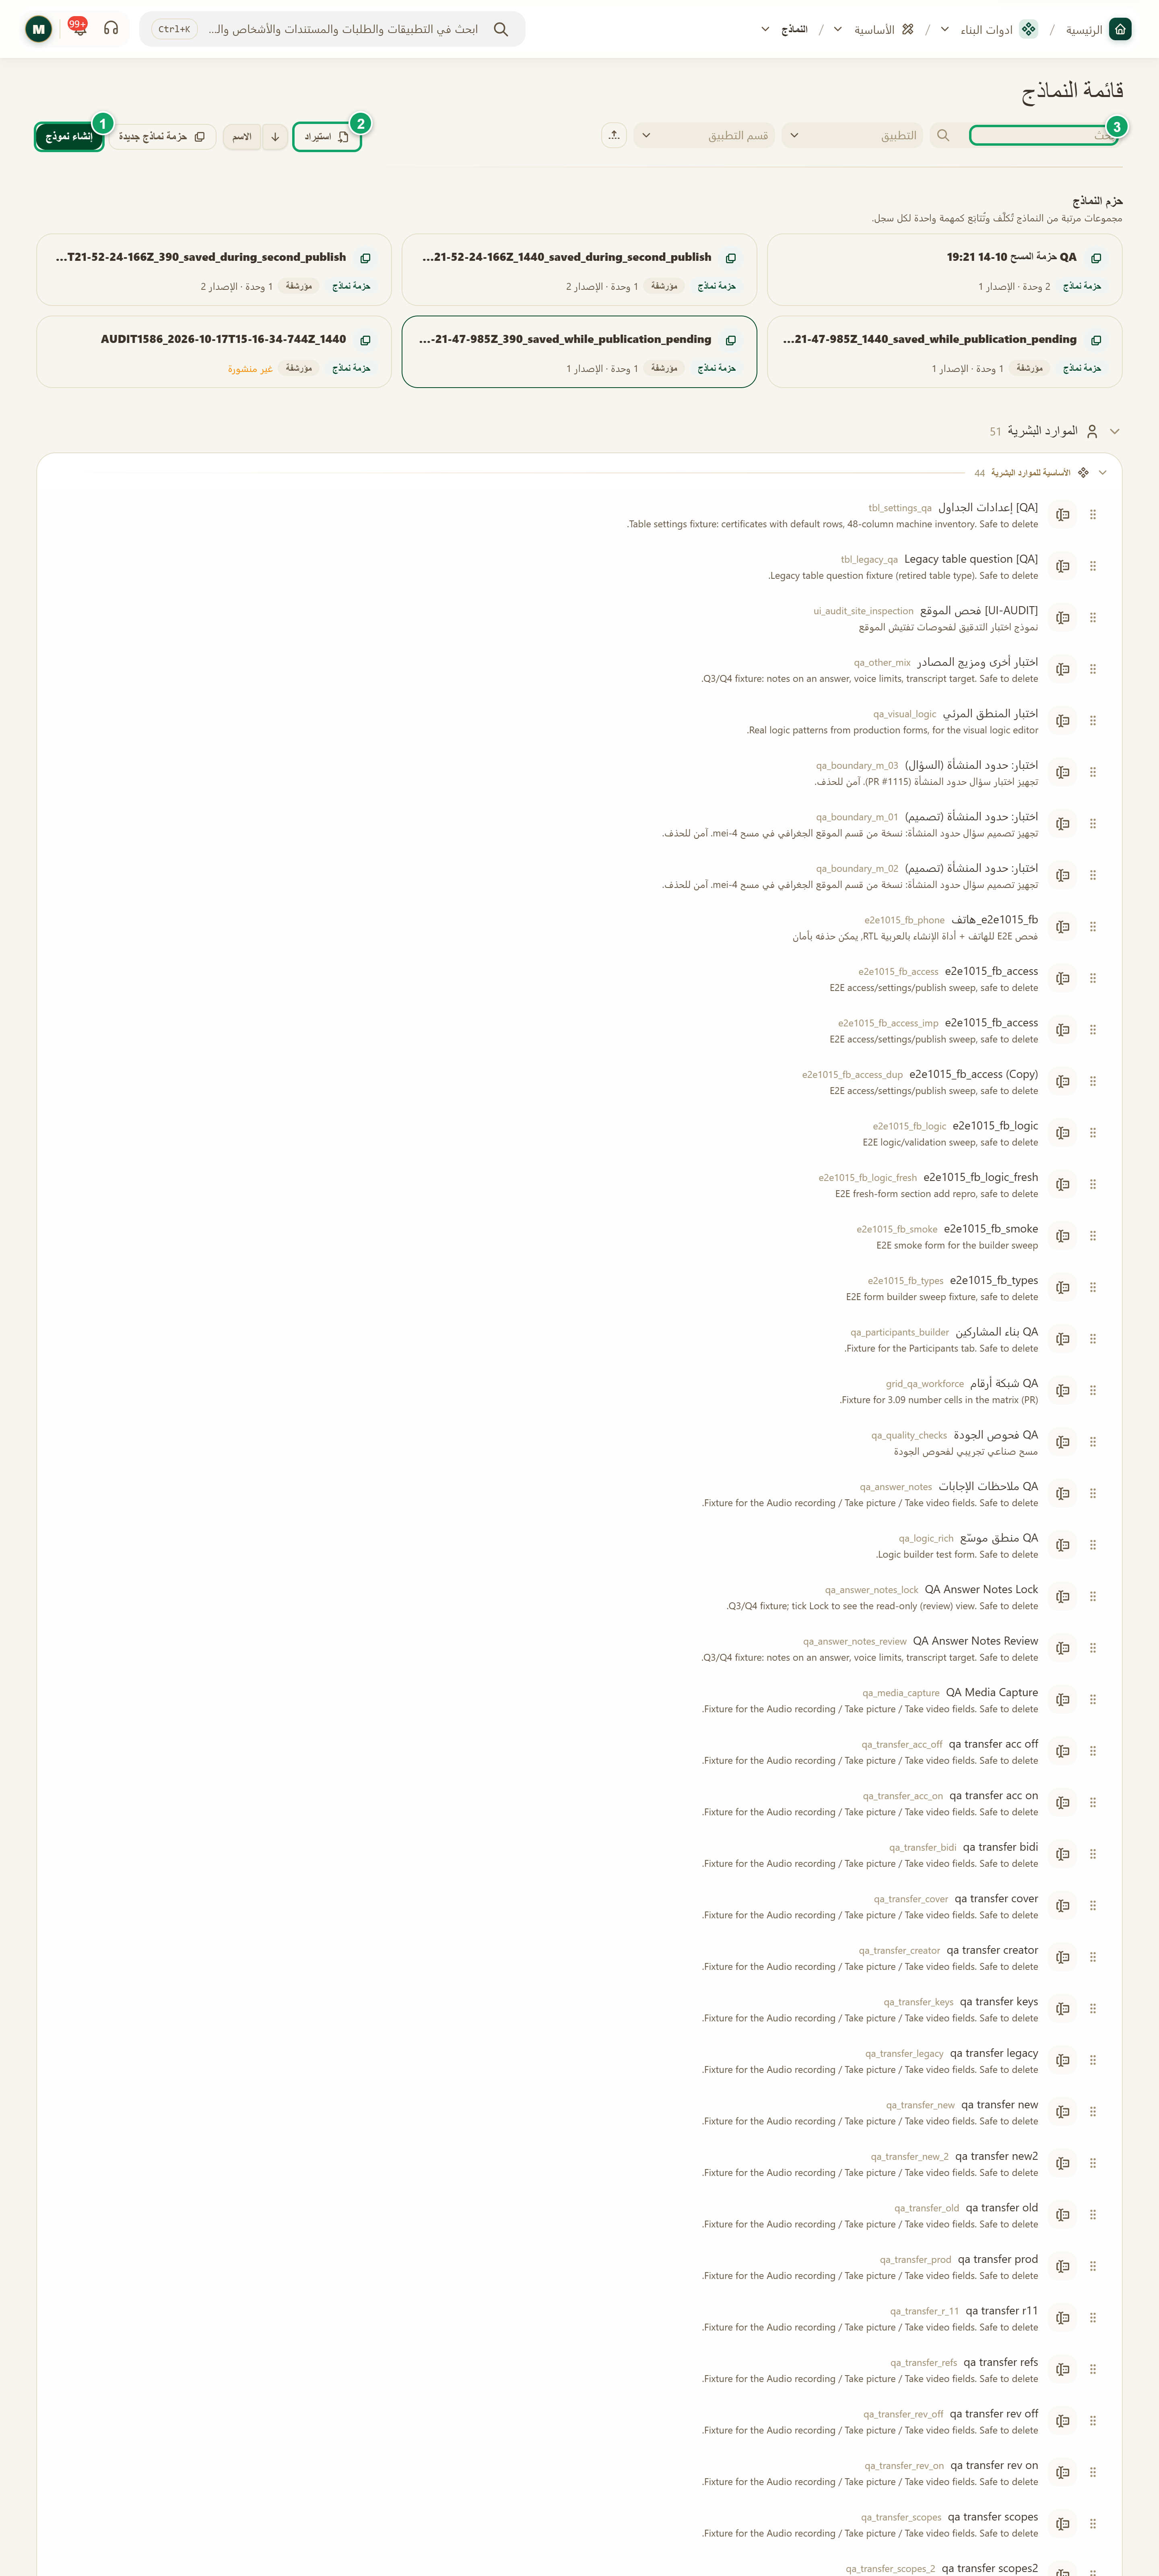
\includegraphics[width=0.95\linewidth,height=0.72\textheight,keepaspectratio]{figures/screens/ch06-forms-ar.png}
\caption{صفحة «النماذج»}
\label{fig:builder-forms-screen}
\shotnote{تعرض الصفحة النماذج مجمّعة حسب التطبيق والقسم مع عدد الطلبات لكل نموذج. والنماذج الظاهرة نماذج اختبار في test2. ① «إنشاء نموذج»: يبدأ نموذجاً جديداً. ② «استيراد»: يُنشئ نموذجاً من ملف مُصدَّر. ③ البحث: يجد النموذج بالاسم.}
\end{figure}


\begin{table}[H]
\centering
\caption{قائمة النماذج}
\label{tab:builder-forms-list}
\begin{tabularx}{\linewidth}{R{3.6cm} Y}
\rcHeaderRow
\thh{الجزء} & \thh{المحتوى والإجراء}\\
إنشاء نموذج & يطلب «اسم النموذج» و«كود النموذج» و«الاختصار المرجعي» والتطبيق والقسم، ثم يفتح المنشئ.\\
القائمة & النماذج مجمّعة حسب التطبيق والقسم، مع البحث والترتيب وعدد الطلبات، وإجراءات «نسخ» و«تصدير النموذج» و«حذف النموذج».\\
استيراد & يُنشئ نموذجاً من ملف مُصدَّر سابقاً.\\
حزم النماذج & مجموعات مرتبة من النماذج تُكلَّف وتُتابَع كمهمة واحدة لكل سجل.\\
\end{tabularx}
\end{table}

\begin{table}[H]
\centering
\caption{أدوات منشئ النموذج}
\label{tab:builder-forms-editor}
\begin{tabularx}{\linewidth}{R{3.6cm} Y}
\rcHeaderRow
\thh{الأداة} & \thh{ماذا تفعل؟}\\
الأسئلة & تضيف الأسئلة من مجموعات: نص، واختيار، وأرقام وتقييم، وتاريخ ووقت، وموقع، والملفات والوسائط، وأخرى؛ مع أقسام وصفحات ونص كتابي.\\
القواعد & كل ما يُظهر سؤالاً أو يخفيه أو يقفله أو يلزم به أو يحسبه أو يتحقق منه، في قائمة واحدة.\\
الوصول & من يستطيع الوصول إلى كل رد، وماذا يستطيع أن يفعل به: من يبدأ النموذج، أو أشخاص ثابتون، أو أشخاص تحددهم الإجابات.\\
المسار & «مسار الطلب»: الحالات والمراحل التي يراها مقدّم الطلب، والانتقالات بينها، وخطوات الموافقة.\\
السجلات & السجلات التي يقرأ منها النموذج ويكتب إليها، ومتى يكتب: «عند الاعتماد» أو «عند الإرسال».\\
إسناد & خطط تكلّف أشخاصاً بتعبئة النموذج لسجلات معينة، وتظهر بعد حفظ النموذج.\\
الإصدارات والإعدادات & «سجل الإصدارات» لكل إصدار، والإعدادات مثل الترقيم ومستند PDF والروابط المملوءة مسبقاً.\\
اختبار النموذج ونشر & يفتح مساحة اختبار معزولة تجرّب فيها النموذج بصفة عضو، ثم «نشر» يجعل المسودة الإصدار المنشور.\\
\end{tabularx}
\end{table}

\begin{figure}[H]
\centering
\begin{tikzpicture}[node distance=0.5cm]
\node[stepBox] (a) {\RL{إنشاء نموذج}};
\node[stepBox,below=of a] (b) {\RL{الأسئلة والقواعد}};
\node[stepBox,below=of b] (c) {\RL{الوصول والمسار والسجلات}};
\node[stepBox,below=of c] (d) {\RL{اختبار النموذج}};
\node[stepBox,below=of d] (e) {\RL{نشر}};
\draw[flowsTo] (a) -- (b);
\draw[flowsTo] (b) -- (c);
\draw[flowsTo] (c) -- (d);
\draw[flowsTo] (d) -- (e);
\end{tikzpicture}
\rclegend
\caption{من الفكرة إلى نموذج منشور}
\label{fig:builder-forms-flow}
\shotnote{يرتّب المخطط بناء النموذج من محتواه إلى سلوكه: الأسئلة أولاً، ثم من يصل إلى الرد وأين تذهب الإجابات. ويأتي الاختبار قبل النشر لأن مساحة الاختبار معزولة، فتكشف الخطأ دون أن يصل إلى أحد؛ أما النشر فيجعل الإصدار متاحاً لكل من يعبّئ النموذج.}
\end{figure}

\subsection{خطوات العمل والتحقق}
\begin{enumerate}
\item افتح «النماذج» واضغط «إنشاء نموذج»، ثم اكتب الاسم والكود والاختصار واختر التطبيق والقسم.
\item أضف الأسئلة، واختر لكل منها نوعاً يناسب الإجابة، ثم أضف القواعد عند الحاجة.
\item افتح «الوصول» لتحدد من يرى الردود، و«السجلات» إن أردت أن تُكتب الإجابات في نوع سجلات.
\item اضغط «اختبار النموذج» وعبّئه كاملاً، ثم اضغط «نشر».
\end{enumerate}

\textbf{تحقق ومعالجة المشكلة:} يجب أن تظهر رسالة «تم نشر النموذج بنجاح»، وأن يظهر الإصدار «منشور» في «سجل الإصدارات». فإذا تحوّل زر النشر إلى «إرسال للاعتماد»، فمؤسستك تشترط اعتماد النشر، وسيُنشر النموذج بعد موافقة المعتمد. وإذا لم تُكتب الإجابات في السجل، فافتح «السجلات» وتأكد من موافقة مسؤول نوع السجلات على كتابة النموذج فيه.


\chapter{الخدمات}
\label{ch:builder-services}

\section{ماذا ستبني في هذا الفصل؟}
\label{sec:builder-services-intro}

الخدمة هي الطريقة التي يصل بها نموذج أو أكثر إلى المتعاملين على بوابة المؤسسة، باسم واضح ودليل يقرؤونه قبل البدء، وشروط تحدد من يحق له التقديم، ورسوم ومسار معروف. ويشرح هذا الفصل إنشاء الخدمة من صفحة «الخدمات»، ثم ضبط تبويبات صفحتها واحداً بعد الآخر: التعريف، والتقديم والأهلية، والمسار والنماذج، والرسوم. ثم ينتقل إلى نشرها على البوابة، واستقبال الطلبات الحضورية في مراكز الخدمة، ومتابعة أداء الطلبات وأماكن تأخرها.

وتسري إعدادات الخدمة على البوابة فور حفظها دون إعادة نشر أي نموذج، أما التعديلات على النموذج نفسه فلا تسري إلا بعد نشره في منشئ النماذج. لذلك ابنِ النموذج وانشره أولاً، ثم أنشئ الخدمة حوله.

\begin{rcnote}[مثال: شركة الأفق]
تريد الأفق أن يطلب عملاؤها زيارة فرع عبر البوابة، فينشئ مسؤول النظام خدمة «طلب زيارة فرع» حول النموذج المنشور بالاسم نفسه، ويجعل الزيارة خطوة حضورية في فرع حلب. ثم يسجّل عمر حداد الطلبات الحضورية في مكتب الاستقبال، وتتابع سارة الخطيب أداء الخدمة وما تأخر من طلباتها.
\end{rcnote}

\section{صفحات هذا الفصل}
\label{sec:builder-services-pages}

تبدأ من صفحة «الخدمات» في قسم «الأساسية» من أدوات البناء، ومنها تفتح كل خدمة في صفحة لها خمسة تبويبات. وترتيب الصفحات هنا هو ترتيب البناء المقترح، فاتبعه في المرة الأولى، ثم عُد إلى أي صفحة عندما تحتاج إليها.

\begin{table}[H]
\centering
\caption{تقديم الخدمات خطوة بخطوة}
\label{tab:builder-pages-services}
\rcZebra
\begin{tabularx}{\linewidth}{R{4.2cm} Y}
\rcHeaderRow
\thh{الصفحة وقسمها} & \thh{ماذا تقدم هذه الصفحة؟}\\
الخدمات — الأساسية & تعرض الخدمات المعروضة على البوابة والنماذج الداخلية، ومنها تنشئ خدمة جديدة وتختار طريقة تقديمها.\\
نظرة عامة على الخدمة — صفحة الخدمة & تلخّص جاهزية الخدمة وأرقامها في آخر 30 يوماً والطلبات المتأخرة وسجل تغييراتها.\\
التعريف ودليل الخدمة — صفحة الخدمة & اسم الخدمة ووصفها وعنوانها على البوابة، والدليل الذي يقرؤه المتعامل قبل أن يبدأ.\\
التقديم والأهلية — صفحة الخدمة & طريقة التقديم وحالة الخدمة، ومن يحق له التقديم وبأي شروط، وحدود الطلبات ومعالجتها.\\
مراكز الخدمة — صفحة الخدمة & الأماكن التي تجري فيها الخطوات الحضورية، وأوقات دوامها، والموظفون الذين يستقبلون فيها.\\
المسار والنماذج — صفحة الخدمة & الخطوات التي يمر بها الطلب بالترتيب، والنماذج خارج المسار، ونماذج المتابعة.\\
الرسوم — صفحة الخدمة & بنود الرسوم ومتى تُستحق، والإعفاءات، وطريقة الدفع وما يحدث للطلب عند الاستحقاق.\\
إتاحة نموذج على البوابة — الخدمات & تحوّل نموذجاً داخلياً منشوراً إلى خدمة جديدة أو إلى خطوة في خدمة قائمة.\\
الخدمة في إعدادات النموذج — منشئ النماذج & تبيّن داخل النموذج الخدمة التي ينتمي إليها، وما تفرضه عليه، ومدى توافقهما.\\
مكتب الاستقبال — الخدمات & يسجّل فيه موظف المركز الطلب الحضوري ويوثّق المستندات المستلمة ويطبع إيصالاً برقم الطلب.\\
أداء الخدمات — الخدمات & يقيس عدد الطلبات ومدد إنجازها، ويبيّن المراحل المتأخرة ورضا المتعاملين.\\
\end{tabularx}
\end{table}

\clearpage
\section{الخدمات}
\label{sec:builder-feature-services}

الخدمة هي ما يظهر للمتعاملين على بوابة المؤسسة، مثل «طلب شهادة» أو «حجز موعد». وتضم كل خدمة نموذجاً أو أكثر، وتحدد طريقة تقديمها ومن يحق له التقديم. لذلك لا يصل النموذج إلى المتعاملين إلا عبر خدمة، أما النموذج الذي لا ينتمي إلى خدمة فيبقى نموذجاً داخلياً يستخدمه الموظفون فقط. وتجمع صفحة «الخدمات» الخدمات كلها في جدول واحد، ومنها تنشئ خدمة جديدة وتفتح مكتب الاستقبال وأداء الخدمات.

\textbf{المسار ومن يستخدمه:} «ادوات البناء» ← «الأساسية» ← «الخدمات». يستخدمها من يدير الخدمات العامة للمؤسسة، عند إنشاء خدمة أو مراجعة حالة الخدمات القائمة.

\begin{rcnote}[مثال: شركة الأفق]
يضغط مسؤول النظام في الأفق «خدمة جديدة» ①، ويسمّي الخدمة «طلب زيارة فرع»، ويختار «هجينة» لأن الطلب يبدأ عبر البوابة وتجري الزيارة نفسها في فرع حلب. ثم يختار النموذج المنشور «طلب زيارة فرع»، بينما تبقى نماذج الأفق الأخرى في «نماذج داخلية» ④.
\end{rcnote}

\begin{figure}[H]
\centering
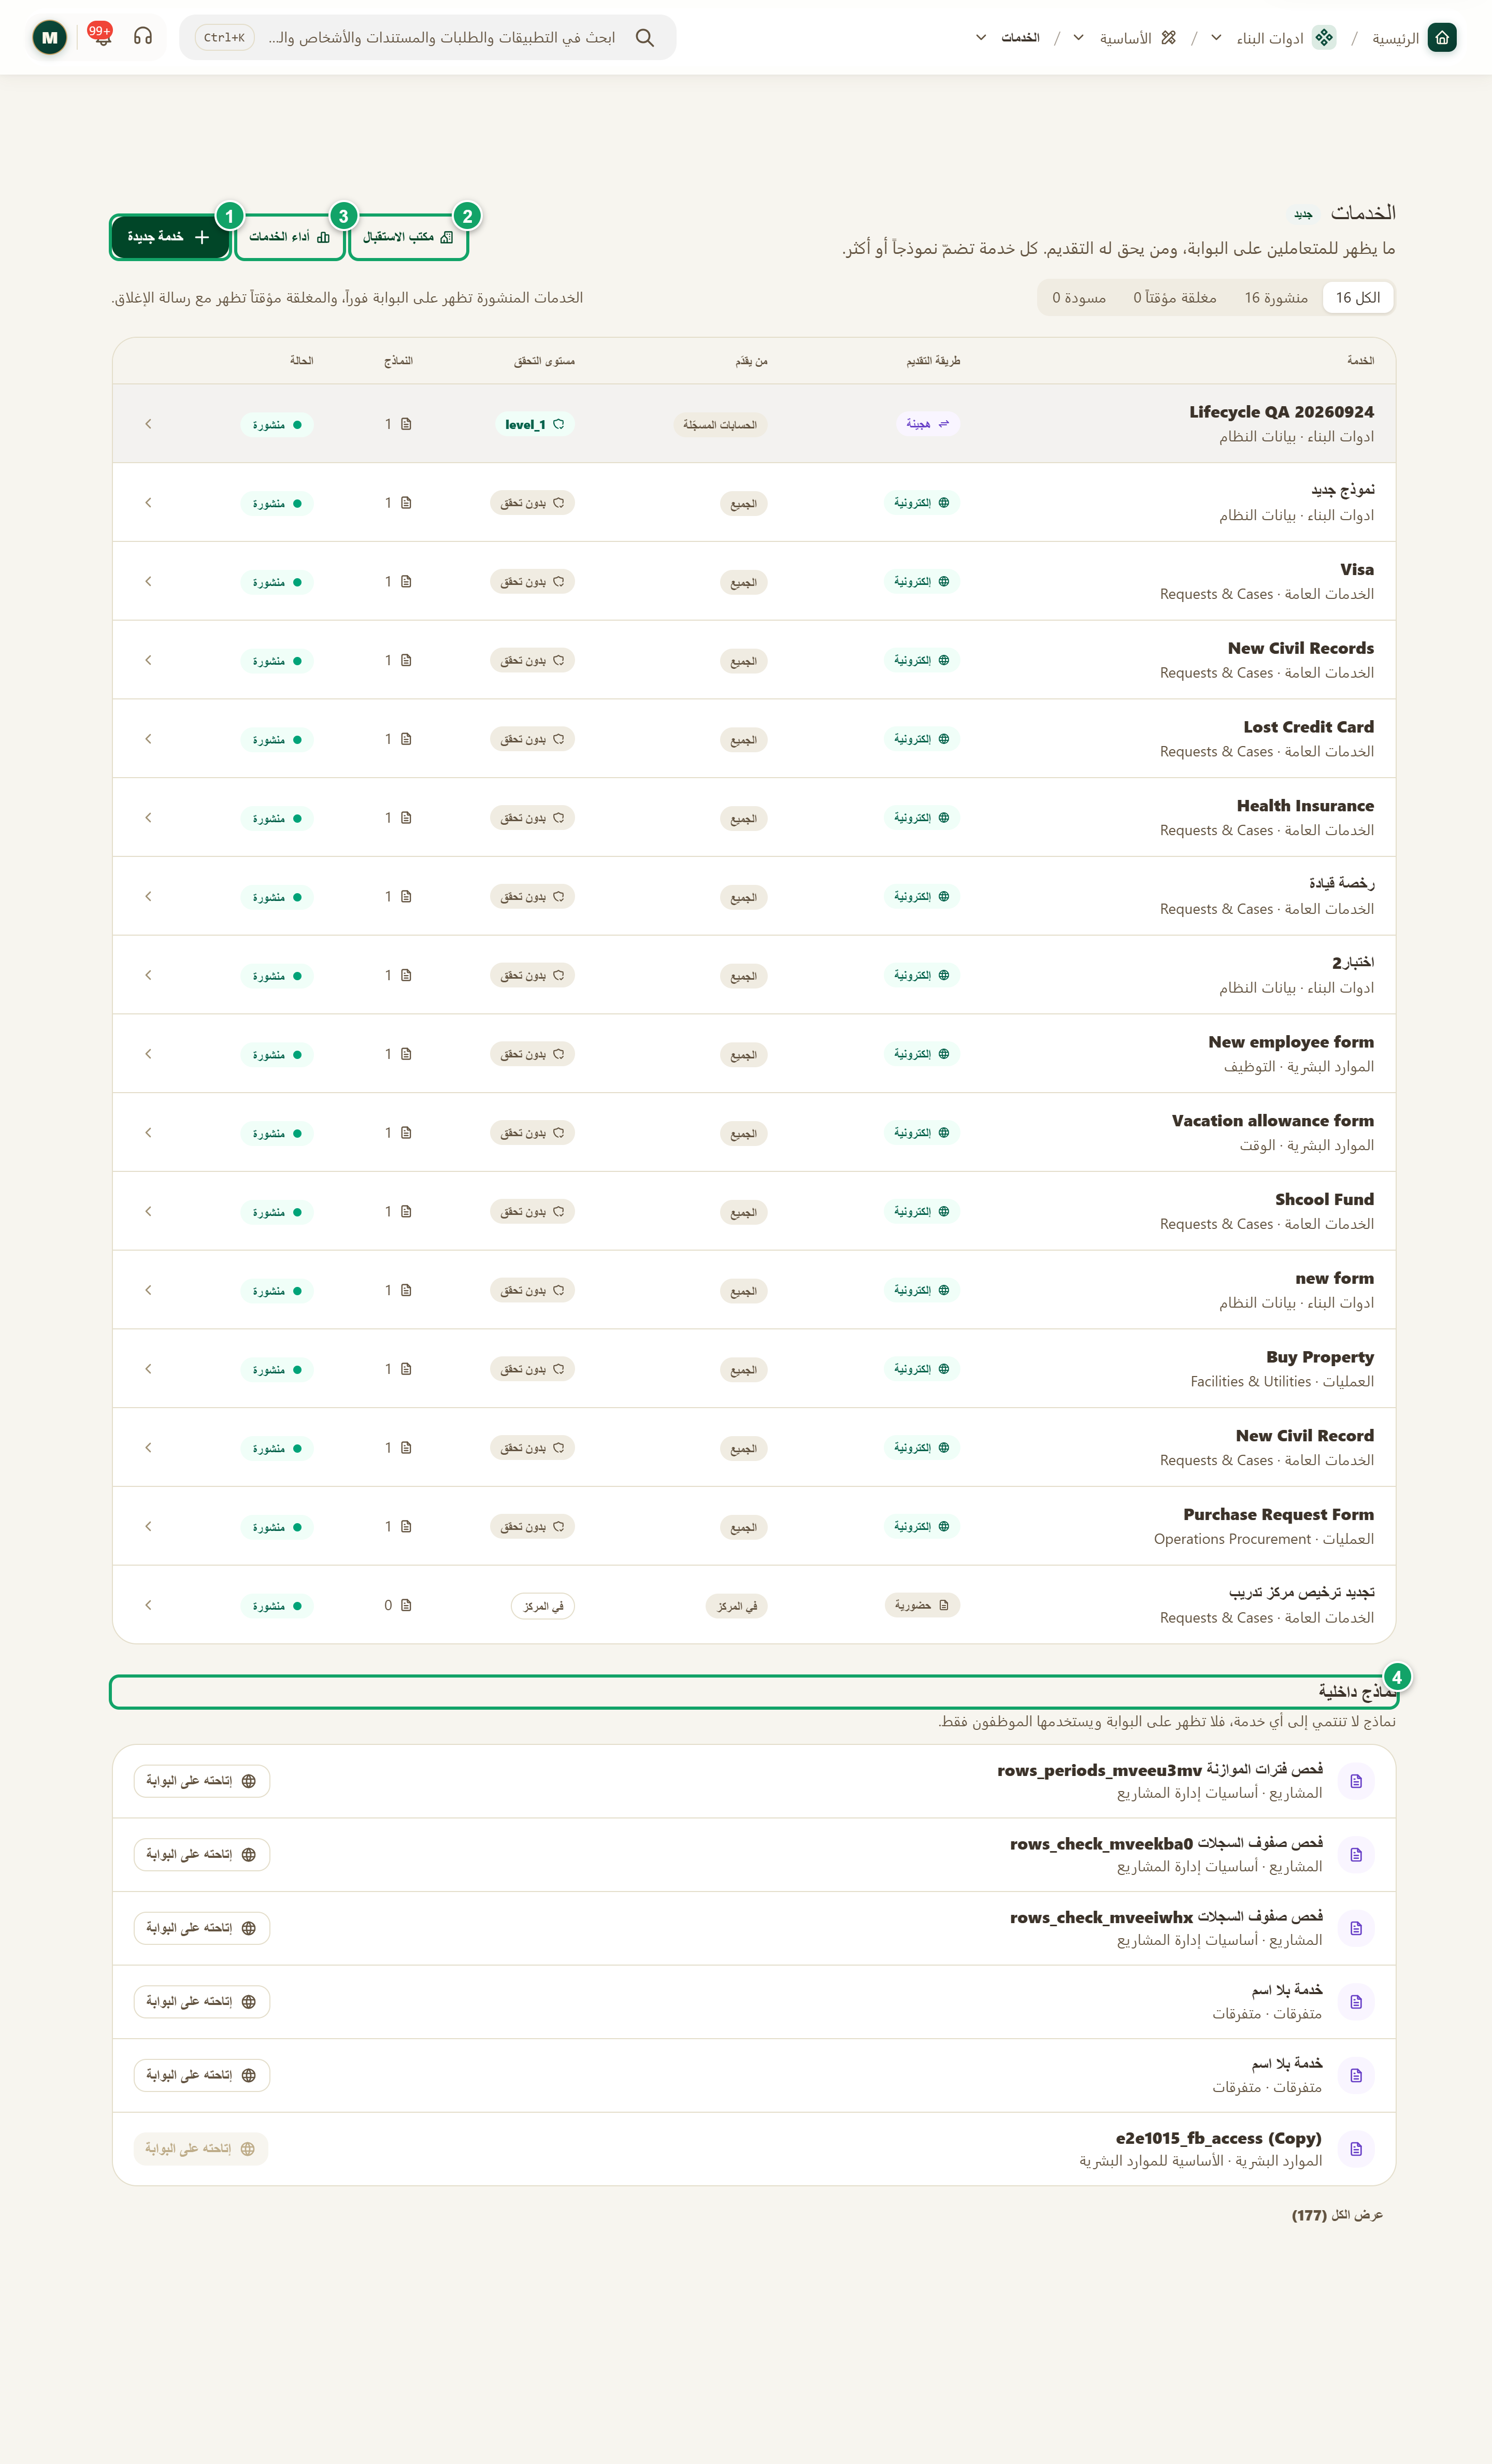
\includegraphics[width=0.95\linewidth,height=0.72\textheight,keepaspectratio]{figures/screens/ch06-services-ar.png}
\caption{صفحة «الخدمات»}
\label{fig:builder-services-screen}
\shotnote{تعرض الصفحة الخدمات التي تظهر على البوابة وحالتها، ثم النماذج الداخلية التي لا تنتمي إلى خدمة. ① «خدمة جديدة»: تبدأ خدمة حول نموذج منشور. ② «مكتب الاستقبال»: يسجّل طلباً حضورياً. ③ «أداء الخدمات». ④ «نماذج داخلية»: النماذج التي لا يراها الجمهور.}
\end{figure}

\begin{figure}[H]
\centering
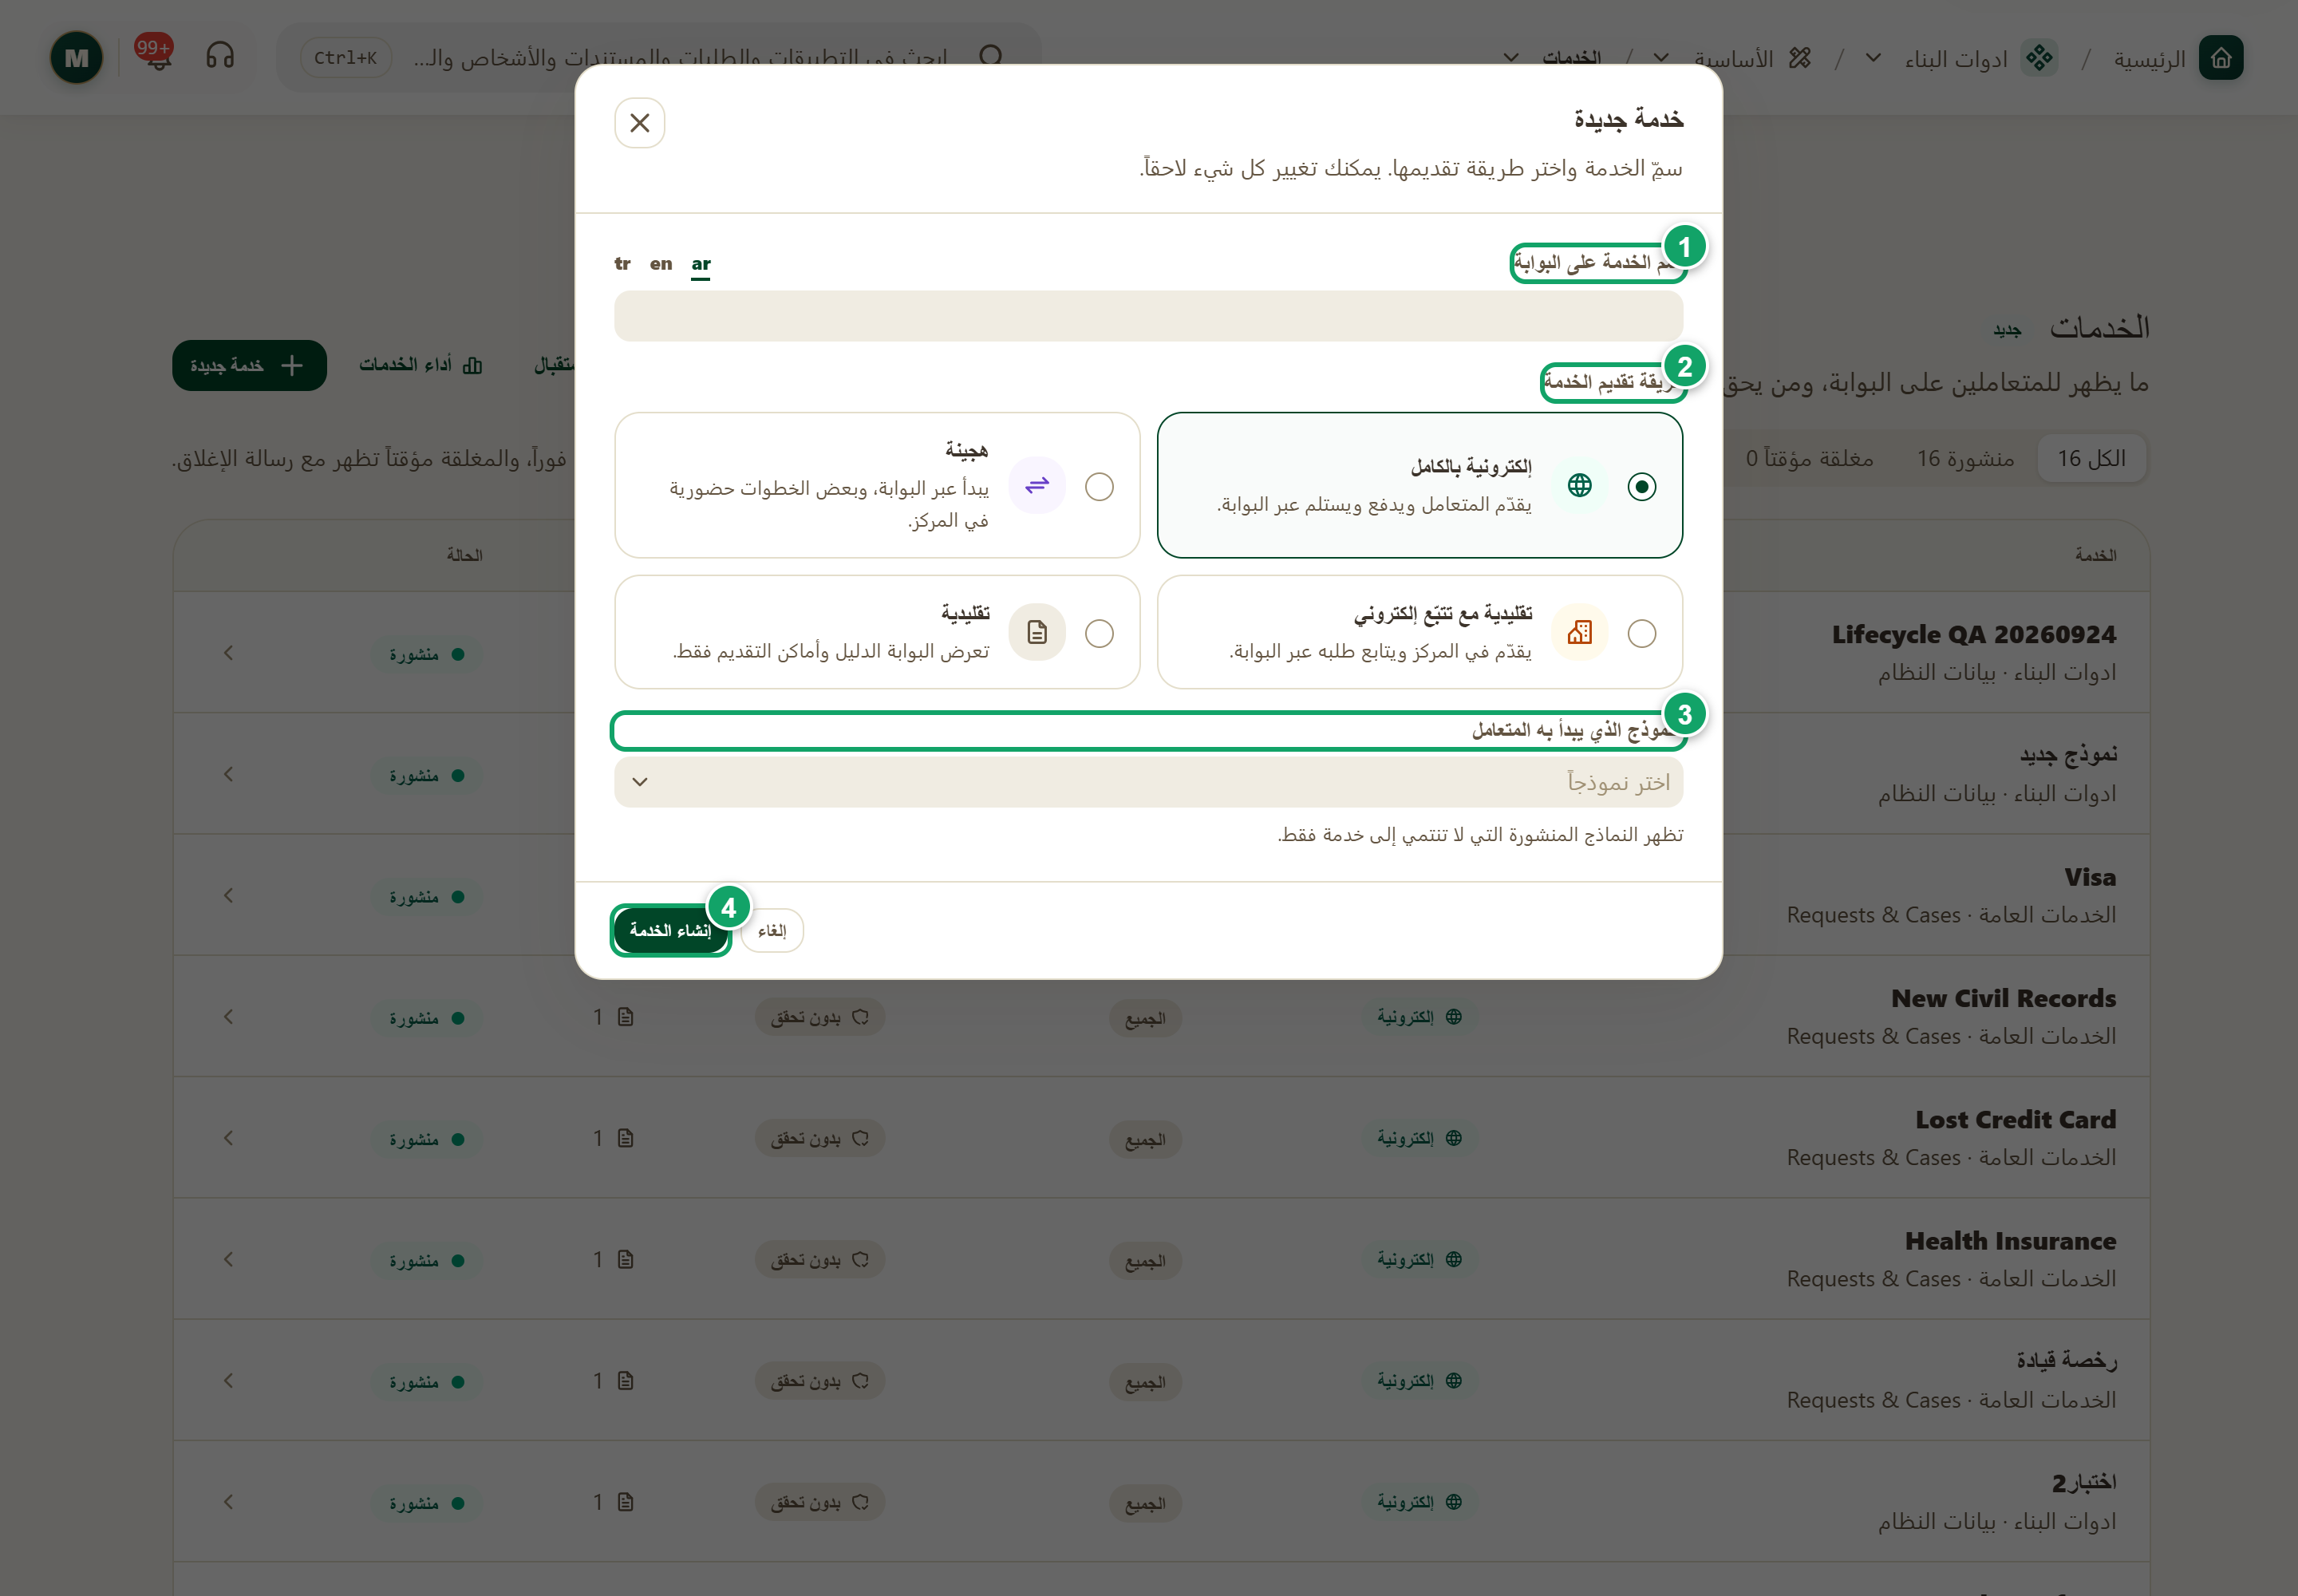
\includegraphics[width=0.95\linewidth,height=0.72\textheight,keepaspectratio]{figures/screens/ch06-services-new-ar.png}
\caption{نافذة «خدمة جديدة»}
\label{fig:builder-services-new-screen}
\shotnote{تعرض الصورة نافذة «خدمة جديدة» قبل تعبئتها في مؤسسة الاختبار، وفيها الطرق الأربع لتقديم الخدمة. وتبيّن أن إنشاء الخدمة لا يطلب سوى ثلاثة أشياء، أما بقية الإعدادات فتُستكمل لاحقاً من صفحة الخدمة. ① «اسم الخدمة على البوابة». ② «طريقة تقديم الخدمة»: تحدد هل تبدأ الخدمة عبر البوابة أو في المركز. ③ «النموذج الذي يبدأ به المتعامل»: لا تعرض القائمة إلا النماذج المنشورة التي لا تنتمي إلى خدمة. ④ «إنشاء الخدمة»: ينشئ الخدمة مسودةً ويفتح صفحتها.}
\end{figure}

\begin{table}[H]
\centering
\caption{ما الذي تجده في صفحة «الخدمات»؟}
\label{tab:builder-services-data}
\begin{tabularx}{\linewidth}{R{3.6cm} Y}
\rcHeaderRow
\thh{الجزء} & \thh{المحتوى والإجراء}\\
جدول الخدمات & يعرض لكل خدمة «طريقة التقديم» و«من يقدّم» و«مستوى التحقق» وعدد «النماذج» و«الحالة»، والضغط على الصف يفتح صفحة الخدمة.\\
تصفية حسب الحالة & تعرض «الكل» أو «منشورة» أو «مغلقة مؤقتاً» أو «مسودة» مع عدد كل منها. والمنشورة تظهر على البوابة فوراً، والمغلقة مؤقتاً تظهر مع رسالة الإغلاق.\\
من إعدادات النموذج & شارة لنموذج منشور للعامة بإعداداته القديمة دون خدمة، وزر «إنشاء خدمة» يحوّله إلى خدمة تديرها من هنا.\\
نماذج داخلية & نماذج لا تنتمي إلى أي خدمة، ولكل منها زر «إتاحته على البوابة» الذي يعمل بعد نشر النموذج.\\
خدمة جديدة & نافذة تطلب «اسم الخدمة على البوابة» و«طريقة تقديم الخدمة» والنموذج الذي تبدأ به الخدمة، ثم تُنشأ الخدمة مسودةً وتفتح صفحتها.\\
\end{tabularx}
\end{table}

\begin{table}[H]
\centering
\caption{طرق تقديم الخدمة}
\label{tab:builder-services-modes}
\begin{tabularx}{\linewidth}{R{3.6cm} Y}
\rcHeaderRow
\thh{الطريقة} & \thh{ما تعنيه وما تطلبه عند الإنشاء}\\
إلكترونية بالكامل & يقدّم المتعامل ويدفع ويستلم عبر البوابة، وكل خطوات المسار نماذج. وتطلب «النموذج الذي يبدأ به المتعامل»، ولا تظهر في القائمة إلا النماذج المنشورة التي لا تنتمي إلى خدمة.\\
هجينة & يبدأ الطلب عبر البوابة، وتجري بعض الخطوات حضورياً في مركز الخدمة. وتطلب نموذج البدء نفسه.\\
تقليدية مع تتبّع إلكتروني & يُقدَّم الطلب في المركز ويتابعه المتعامل على البوابة برقم الطلب ورقم الهاتف. ويمكنك أن تختار «نموذج يعبّئه الموظف (اختياري)».\\
تقليدية & لا طلبات على البوابة، بل تعرض الدليل وأماكن التقديم فقط، ويمكن للموظفين تسجيل الطلب داخلياً. والنموذج هنا اختياري أيضاً.\\
\end{tabularx}
\end{table}

\begin{figure}[H]
\centering
\begin{tikzpicture}[node distance=0.5cm]
\node[entity] (service) {\RL{الخدمة}};
\node[entity,below right=0.7cm and 0.3cm of service] (entry) {\RL{نموذج البداية}};
\node[entityOpt,below left=0.7cm and 0.3cm of service] (more) {\RL{نماذج المسار والمتابعة}};
\draw[dependsOn] (service.south) -- ++(0,-0.3) -| (entry.north);
\draw[dependsOnOpt] (service.south) -- ++(0,-0.3) -| (more.north);
\end{tikzpicture}
\rclegend
\caption{ما تضمه الخدمة}
\label{fig:builder-services-model}
\shotnote{يوضّح الشكل أن الخدمة التي تبدأ عبر البوابة تحتاج إلى نموذج بداية منشور يعبّئه المتعامل، وأن بقية النماذج اختيارية، مثل خطوات لاحقة في المسار أو نموذج متابعة يُطلب عند حالة معينة. لذلك انشر النموذج في منشئ النماذج أولاً، ثم أنشئ الخدمة حوله.}
\end{figure}

\subsection{خطوات العمل والتحقق}
\begin{enumerate}
\item انشر النموذج الذي سيبدأ به المتعامل من صفحة «النماذج».
\item افتح «الخدمات» واضغط «خدمة جديدة»، واكتب «اسم الخدمة على البوابة».
\item اختر «طريقة تقديم الخدمة»، ثم اختر النموذج من القائمة واضغط «إنشاء الخدمة».
\item أكمل تبويبات صفحة الخدمة: «التعريف» و«التقديم والأهلية» و«المسار والنماذج» و«الرسوم».
\item غيّر «حالة الخدمة» إلى «منشورة»، ثم اضغط «عرض على البوابة» لتراها كما يراها المتعامل.
\end{enumerate}

\textbf{تحقق ومعالجة المشكلة:} تظهر الخدمة الجديدة في الجدول بحالة «مسودة»، ولا تظهر على البوابة حتى تنشرها، لأن «المسودة لا تظهر على البوابة». وإذا لم تجد نموذجك في قائمة الإنشاء، فتأكد من أنه منشور ولا ينتمي إلى خدمة أخرى. وإذا أردت إيقاف الطلبات مؤقتاً، فاجعل الخدمة «مغلقة مؤقتاً» مع رسالة للمتعاملين بدلاً من حذفها.

\clearpage
\section{نظرة عامة على الخدمة}
\label{sec:builder-feature-services-overview}

تفتح كل خدمة على تبويب «نظرة عامة»، وهو ملخص يجيب عن ثلاثة أسئلة: هل الخدمة جاهزة، وكيف يسير أداؤها، وما الذي يحتاج إلى تدخلك الآن. وتبدأ الصفحة بقائمة «جاهزية الخدمة» التي تفحص كل جزء من إعدادها، ثم أرقام آخر 30 يوماً، ثم الطلبات المتأخرة. لذلك عُد إليها كلما فتحت الخدمة لتعرف أين تبدأ.

\textbf{المسار ومن يستخدمه:} «الخدمات» ← اضغط الخدمة ← «نظرة عامة». يستخدمها من يبني الخدمة ليكمل إعدادها، ومن يتابعها ليرى ما تأخر من طلباتها.

\begin{rcnote}[مثال: شركة الأفق]
يفتح مسؤول النظام خدمة «طلب زيارة فرع» فيجد في «جاهزية الخدمة» ① أن «الرسوم» غير معدّة وأن «الاستقبال في المركز» متوقف. فيضغط «تفعيل» بجانب الاستقبال لينتقل مباشرة إلى تبويب «التقديم والأهلية».
\end{rcnote}

\begin{figure}[H]
\centering
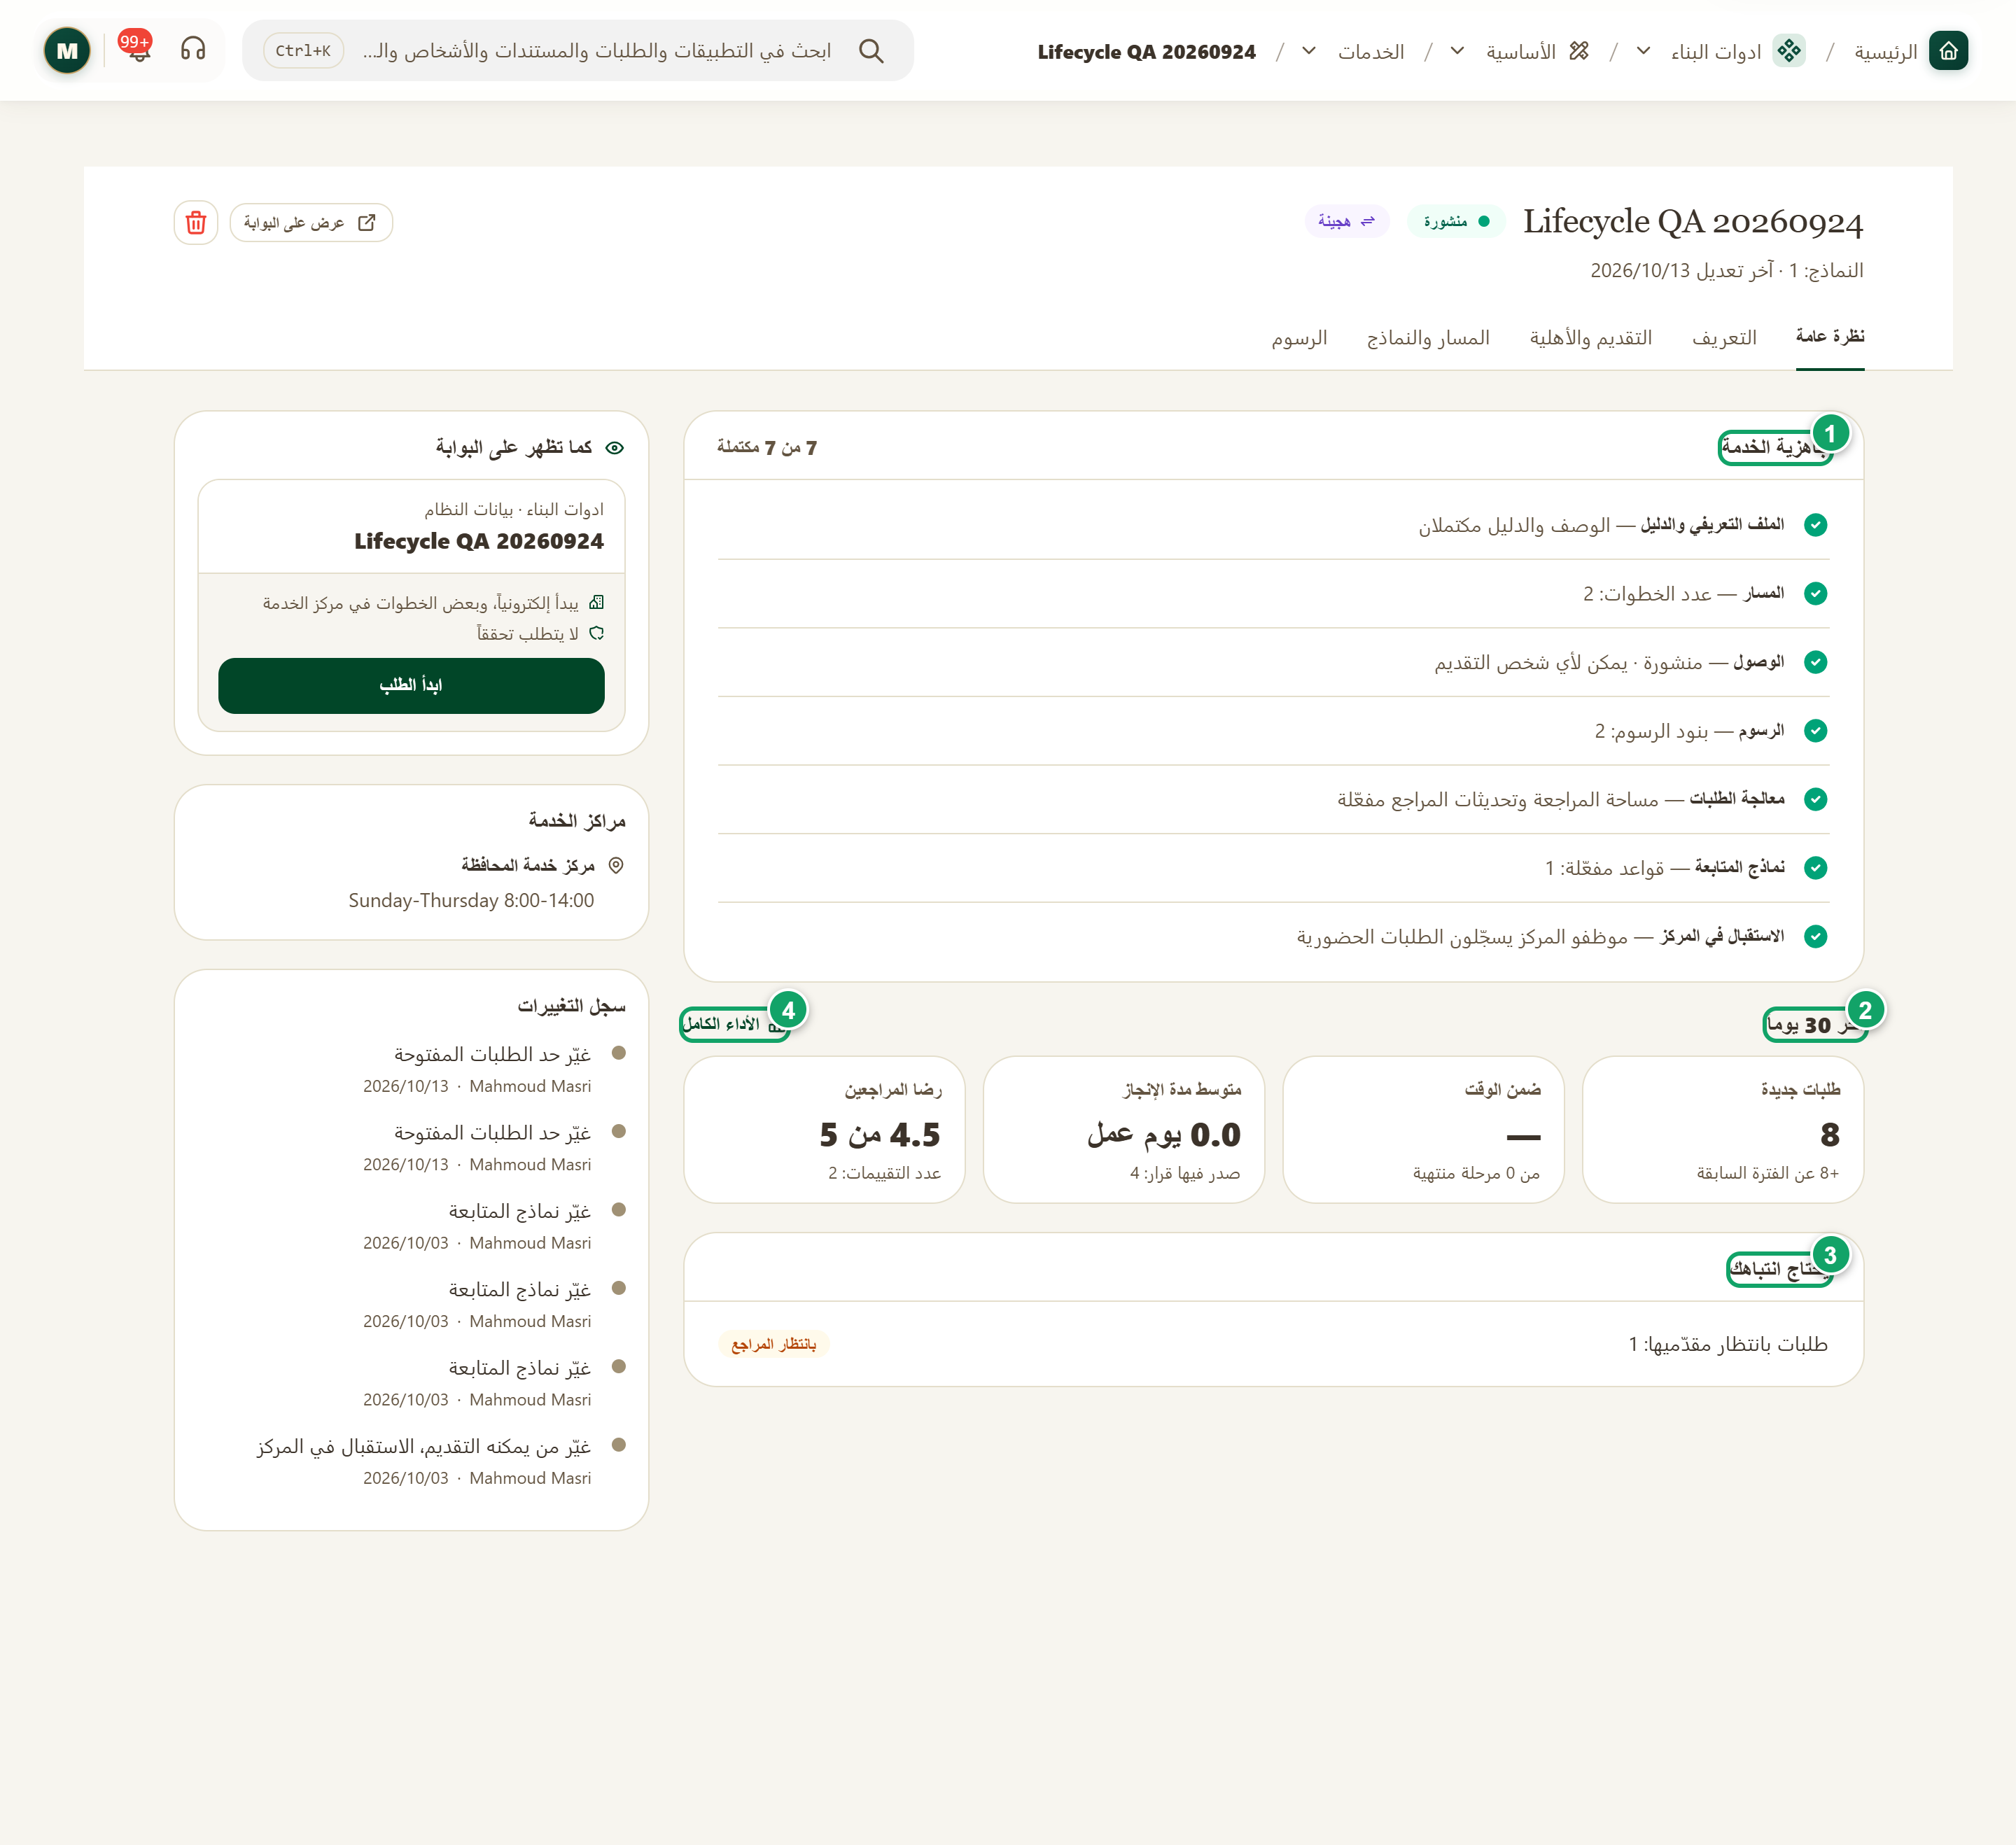
\includegraphics[width=0.95\linewidth,height=0.72\textheight,keepaspectratio]{figures/screens/ch06-services-overview-ar.png}
\caption{تبويب «نظرة عامة» لخدمة في مؤسسة الاختبار}
\label{fig:builder-services-overview-screen}
\shotnote{تعرض الصورة خدمة هجينة منشورة في مؤسسة الاختبار اكتملت بنود جاهزيتها السبعة، ومعها أرقام آخر 30 يوماً وطلب واحد ينتظر مقدّمه. وتبيّن أن هذا التبويب يجمع حالة الإعداد وحالة الطلبات في شاشة واحدة، فتعرف منه ما يحتاج إلى إكمال وما يحتاج إلى متابعة. ① «جاهزية الخدمة»: البنود التي تفحص إعداد الخدمة مع عدّاد المكتمل منها. ② «آخر 30 يوماً». ③ «يحتاج انتباهك»: الطلبات المتأخرة أو التي تنتظر مقدّميها. ④ «الأداء الكامل»: يفتح صفحة «أداء الخدمات».}
\end{figure}

\begin{table}[H]
\centering
\caption{بنود «جاهزية الخدمة»}
\label{tab:builder-services-overview-checks}
\begin{tabularx}{\linewidth}{R{3.6cm} Y}
\rcHeaderRow
\thh{البند} & \thh{متى يكتمل}\\
الملف التعريفي والدليل & عندما يكون للخدمة وصف، ومعه مدة الإنجاز أو مستند مطلوب واحد على الأقل في الدليل.\\
المسار & عندما يضم المسار خطوة واحدة على الأقل، ويظهر عدد الخطوات.\\
الوصول & عندما تكون الخدمة «منشورة»، ويذكر البند أيضاً هل تتطلب حساباً ومستوى التحقق المطلوب.\\
الرسوم & عندما تُفعَّل بنود الرسوم وفيها بند واحد على الأقل. أما إذا كُتبت الرسوم نصاً في الدليل فقط، فينبّهك البند إلى تحويلها إلى بنود.\\
معالجة الطلبات & عندما تُفعَّل مساحة المراجعة وتحديثات المراجع لنموذج البدء.\\
نماذج المتابعة & عندما تُفعَّل نماذج المتابعة، ويظهر عدد القواعد المفعّلة.\\
الاستقبال في المركز & يظهر للخدمات التي فيها خطوات حضورية فقط، ويكتمل عندما يسجّل موظفو المركز الطلبات الحضورية.\\
\end{tabularx}
\end{table}

وبجانب كل بند غير مكتمل رابط ينقلك إلى التبويب الذي يصلحه، مثل «استكمال» أو «فتح الرسوم» أو «إعداد» أو «تفعيل».

\begin{table}[H]
\centering
\caption{بقية أجزاء «نظرة عامة»}
\label{tab:builder-services-overview-parts}
\begin{tabularx}{\linewidth}{R{3.6cm} Y}
\rcHeaderRow
\thh{الجزء} & \thh{ما يعرضه}\\
آخر 30 يوماً & أربعة مؤشرات: «طلبات جديدة» مقارنة بالفترة السابقة، و«ضمن الوقت»، و«متوسط مدة الإنجاز» بأيام العمل، و«رضا المراجعين» من 5. ورابط «الأداء الكامل» يفتح صفحة «أداء الخدمات».\\
يحتاج انتباهك & حتى خمسة طلبات متأخرة مع المرحلة التي تأخرت فيها وعدد أيام التأخر، وعدد الطلبات التي تنتظر مقدّميها.\\
كما تظهر على البوابة & معاينة بطاقة الخدمة كما يراها المتعامل، أو تنبيه بأن المسودة لا تظهر على البوابة.\\
مراكز الخدمة & المراكز التي اختارتها الخدمة مع أوقات دوامها.\\
سجل التغييرات & من غيّر ماذا ومتى، مثل «غيّر الرسوم» أو «أنشأ الخدمة».\\
\end{tabularx}
\end{table}

\begin{figure}[H]
\centering
\begin{tikzpicture}[node distance=0.5cm]
\node[stepBox] (a) {\RL{قراءة جاهزية الخدمة}};
\node[stepBox,below=of a] (b) {\RL{فتح التبويب الناقص}};
\node[stepBox,below=of b] (c) {\RL{الحفظ والعودة}};
\node[stepBox,below=of c] (d) {\RL{مراجعة يحتاج انتباهك}};
\draw[flowsTo] (a) -- (b);
\draw[flowsTo] (b) -- (c);
\draw[flowsTo] (c) -- (d);
\end{tikzpicture}
\rclegend
\caption{استخدام «نظرة عامة» في كل زيارة للخدمة}
\label{fig:builder-services-overview-flow}
\shotnote{يبدأ المخطط بالجاهزية لأنها تدلك على التبويب الذي يحتاج إلى إكمال، ثم تعود بعد الحفظ لترى البند مكتملاً. أما «يحتاج انتباهك» فيأتي أخيراً لأنه يخص الطلبات الجارية، لا إعداد الخدمة نفسها.}
\end{figure}

\subsection{خطوات العمل والتحقق}
\begin{enumerate}
\item افتح «الخدمات» واضغط الخدمة، فتفتح على «نظرة عامة».
\item اقرأ العدّاد بجانب «جاهزية الخدمة»، مثل «5 من 7 مكتملة».
\item اضغط الرابط بجانب أول بند غير مكتمل، وأكمل التبويب الذي ينقلك إليه، ثم اضغط «حفظ وتطبيق».
\item عُد إلى «نظرة عامة» وراجع «يحتاج انتباهك»، واضغط «فتح» بجانب أي طلب متأخر لتعالجه.
\end{enumerate}

\textbf{تحقق ومعالجة المشكلة:} بعد الحفظ يتحول البند إلى «مكتمل» ويزيد العدّاد. وإذا ظهر «تعذّر تحميل الأرقام.»، فأعد تحميل الصفحة؛ فهذا لا يؤثر في إعداد الخدمة. أما الخدمة التي تحمل شارة «من إعدادات النموذج» فلا تظهر لها أرقام حتى تحوّلها إلى خدمة.

\clearpage
\section{التعريف ودليل الخدمة}
\label{sec:builder-feature-services-profile}

تبويب «التعريف» هو ما يقرؤه المتعامل قبل أن يبدأ: اسم الخدمة ووصفها، ودليلها الذي يذكر المدة والرسوم والمستندات المطلوبة. فكلما كان الدليل أوضح قلّت الطلبات الناقصة والأسئلة المتكررة. ويحدد التبويب أيضاً عنوان الخدمة على البوابة والمكان الذي تظهر فيه بين التطبيقات والأقسام.

\textbf{المسار ومن يستخدمه:} «الخدمات» ← اضغط الخدمة ← «التعريف». يملؤه من يبني الخدمة، ويعدّله من يتابع أسئلة المتعاملين حين يتغير شيء في الإجراءات.

\begin{rcnote}[مثال: شركة الأفق]
يكتب مسؤول النظام في «مدة الإنجاز» عبارة «3 أيام عمل»، ويضيف بزر «إضافة مستند» ③ صورة الهوية مستنداً إلزامياً. ثم يختار في «مكان العرض على البوابة» ④ تطبيق «خدمات الفروع» ليجد العملاء الخدمة فيه.
\end{rcnote}

\begin{figure}[H]
\centering
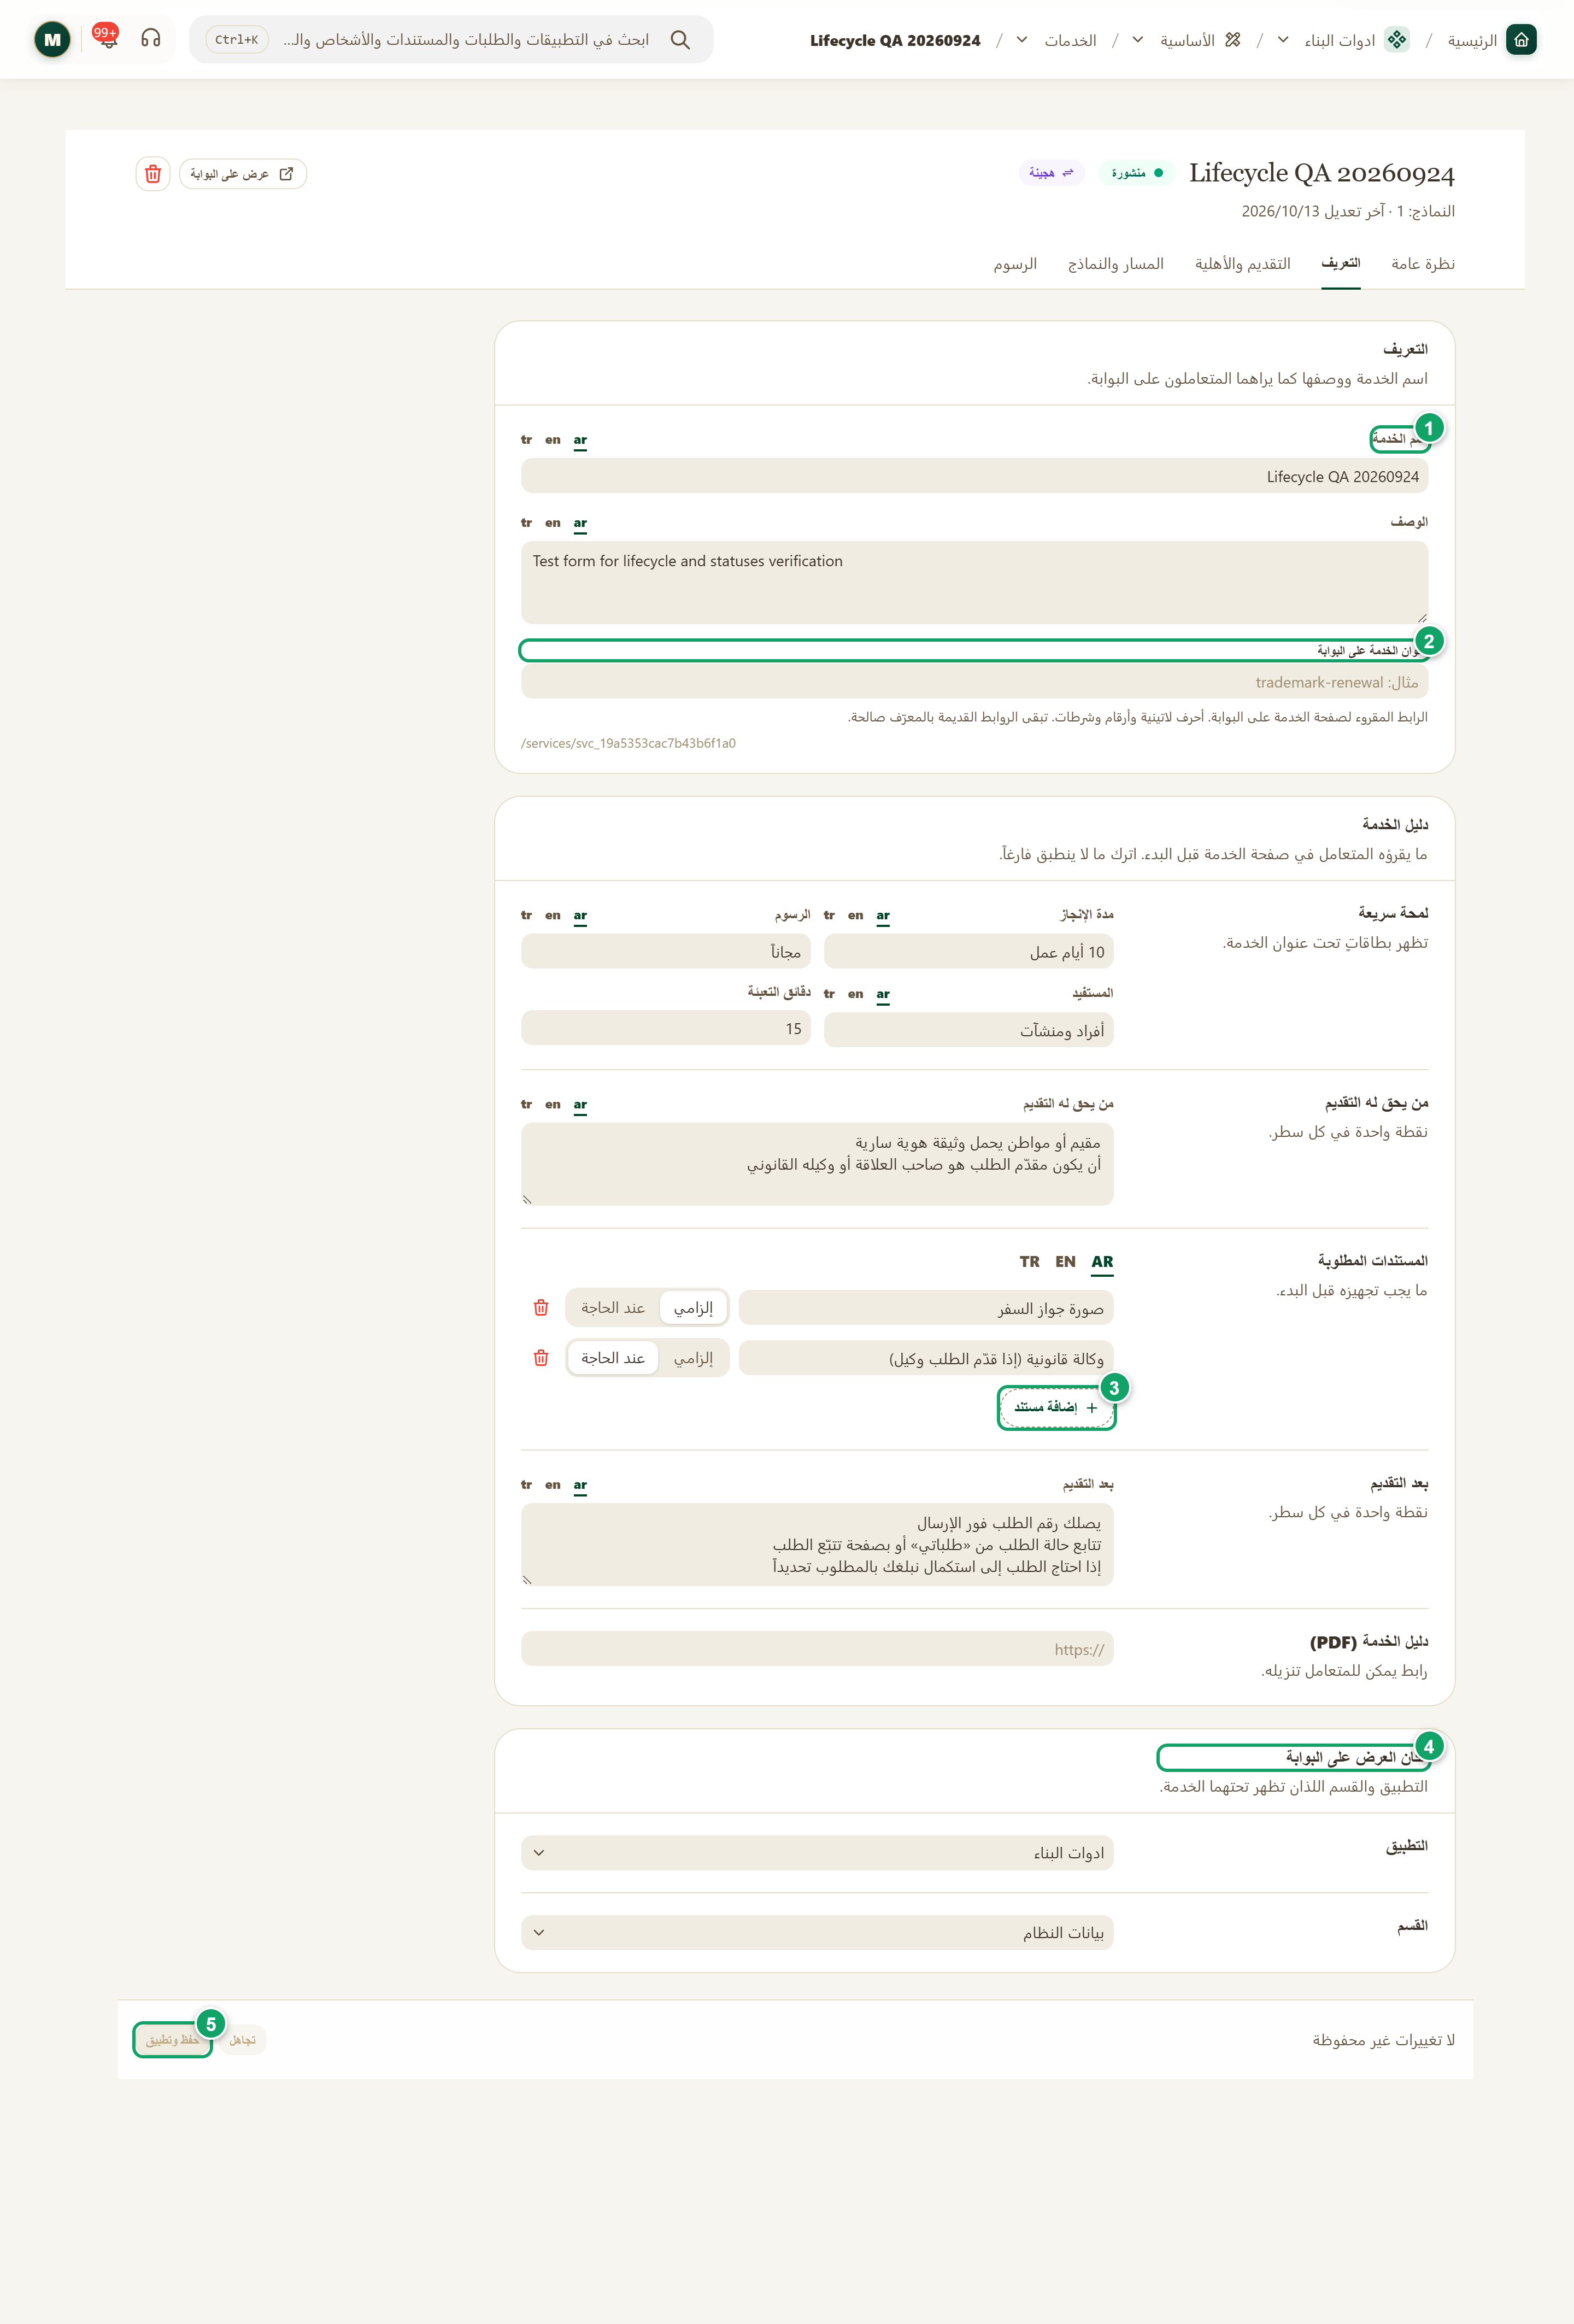
\includegraphics[width=0.95\linewidth,height=0.72\textheight,keepaspectratio]{figures/screens/ch06-services-profile-ar.png}
\caption{تبويب «التعريف» ودليل الخدمة}
\label{fig:builder-services-profile-screen}
\shotnote{تعرض الصورة تبويب «التعريف» لخدمة في مؤسسة الاختبار، وفيها حقول «لمحة سريعة» و«المستندات المطلوبة» ما زالت فارغة. وتوضح أن ما يقرؤه المتعامل قبل أن يبدأ يُكتب كله هنا، ثم يسري على البوابة بزر واحد. ① «اسم الخدمة». ② «عنوان الخدمة على البوابة»: رابط مقروء اختياري لصفحة الخدمة. ③ «إضافة مستند»: يضيف مستنداً مطلوباً وتحدد له «إلزامي» أو «عند الحاجة». ④ «مكان العرض على البوابة»: التطبيق والقسم اللذان تظهر تحتهما الخدمة. ⑤ «حفظ وتطبيق»: يحفظ التعريف ويُعطَّل حتى تغيّر شيئاً.}
\end{figure}

\begin{table}[H]
\centering
\caption{أقسام تبويب «التعريف»}
\label{tab:builder-services-profile-parts}
\begin{tabularx}{\linewidth}{R{3.6cm} Y}
\rcHeaderRow
\thh{القسم} & \thh{ما تكتبه فيه}\\
التعريف & «اسم الخدمة» وهو مطلوب، و«الوصف» الذي يذكر لمن الخدمة وما يحصل عليه المتعامل.\\
عنوان الخدمة على البوابة & الرابط المقروء لصفحة الخدمة، من 3 إلى 80 حرفاً لاتينياً صغيراً أو رقماً مع شرطات، مثل \en{branch-visit}. وتبقى الروابط القديمة بالمعرّف صالحة.\\
دليل الخدمة & «لمحة سريعة» تظهر بطاقاتٍ تحت العنوان: «مدة الإنجاز» و«الرسوم» و«المستفيد» و«دقائق التعبئة». ثم «من يحق له التقديم» و«المستندات المطلوبة» و«بعد التقديم» و«دليل الخدمة (PDF)».\\
مكان العرض على البوابة & «التطبيق» و«القسم» اللذان تظهر تحتهما الخدمة.\\
\end{tabularx}
\end{table}

ولكل مستند في «المستندات المطلوبة» نوع: «إلزامي» أو «عند الحاجة». وتهمّك هذه القائمة لاحقاً، لأن مكتب الاستقبال يعرضها على موظف المركز ليؤشّر ما استلمه من المتعامل. واترك فارغاً ما لا ينطبق على خدمتك.

\begin{figure}[H]
\centering
\begin{tikzpicture}[node distance=0.5cm]
\node[stepBox] (a) {\RL{الاسم والوصف}};
\node[stepBox,below=of a] (b) {\RL{لمحة سريعة}};
\node[stepBox,below=of b] (c) {\RL{المستندات المطلوبة}};
\node[stepBox,below=of c] (d) {\RL{مكان العرض على البوابة}};
\node[stepBox,below=of d] (e) {\RL{حفظ وتطبيق}};
\draw[flowsTo] (a) -- (b);
\draw[flowsTo] (b) -- (c);
\draw[flowsTo] (c) -- (d);
\draw[flowsTo] (d) -- (e);
\end{tikzpicture}
\rclegend
\caption{إكمال تعريف الخدمة}
\label{fig:builder-services-profile-flow}
\shotnote{يرتّب المخطط الأقسام كما يقرؤها المتعامل: الاسم والوصف أولاً، ثم المدة والرسوم، ثم ما يجب أن يجهّزه. وينتهي بالحفظ لأن التغييرات تسري على البوابة فوره، دون إعادة نشر أي نموذج.}
\end{figure}

\subsection{خطوات العمل والتحقق}
\begin{enumerate}
\item افتح الخدمة واضغط تبويب «التعريف».
\item اكتب «اسم الخدمة» و«الوصف»، وأضف «عنوان الخدمة على البوابة» إن أردت رابطاً مقروءاً.
\item املأ «لمحة سريعة»، ثم أضف المستندات بزر «إضافة مستند» وحدد لكل منها «إلزامي» أو «عند الحاجة».
\item اختر «التطبيق» و«القسم» في «مكان العرض على البوابة»، ثم اضغط «حفظ وتطبيق».
\end{enumerate}

\textbf{تحقق ومعالجة المشكلة:} يتغير شريط الحفظ إلى «لا تغييرات غير محفوظة»، ويصبح بند «الملف التعريفي والدليل» مكتملاً في «نظرة عامة». فإذا بقي زر الحفظ معطلاً، فتحقق من أن «اسم الخدمة» غير فارغ وأن العنوان يطابق الشرط المكتوب تحته. وإذا ظهر «هذا العنوان مستخدم لخدمة أخرى.»، فاختر عنواناً مختلفاً.

\clearpage
\section{التقديم والأهلية}
\label{sec:builder-feature-services-delivery}

يحدد تبويب «التقديم والأهلية» كيف تُقدَّم الخدمة، ومتى تكون متاحة، ومن يحق له التقديم وبأي شروط. وبذلك يمنع الطلبات التي لا تستوفي الشروط قبل أن تبدأ، بدلاً من رفضها بعد وصولها. وتختلف الأقسام الظاهرة بحسب طريقة التقديم: فالخدمة التي تبدأ عبر البوابة تعرض أقسام الأهلية والتحقق، والخدمة التي فيها خطوات حضورية تعرض مراكز الخدمة والمواعيد والاستقبال.

\textbf{المسار ومن يستخدمه:} «الخدمات» ← اضغط الخدمة ← «التقديم والأهلية». يضبطه من يبني الخدمة، ويعود إليه لإغلاقها مؤقتاً أو لتغيير شروطها.

\begin{rcnote}[مثال: شركة الأفق]
يختار مسؤول النظام لخدمة «طلب زيارة فرع» «أصحاب الحسابات المسجّلة فقط» ③، ويحدد «الطلبات المفتوحة لكل متعامل» بطلب واحد حتى لا يكرر العميل الطلب نفسه. ثم يختار فرع حلب في «مراكز الخدمة» ويفعّل «الاستقبال في المركز».
\end{rcnote}

\begin{figure}[H]
\centering
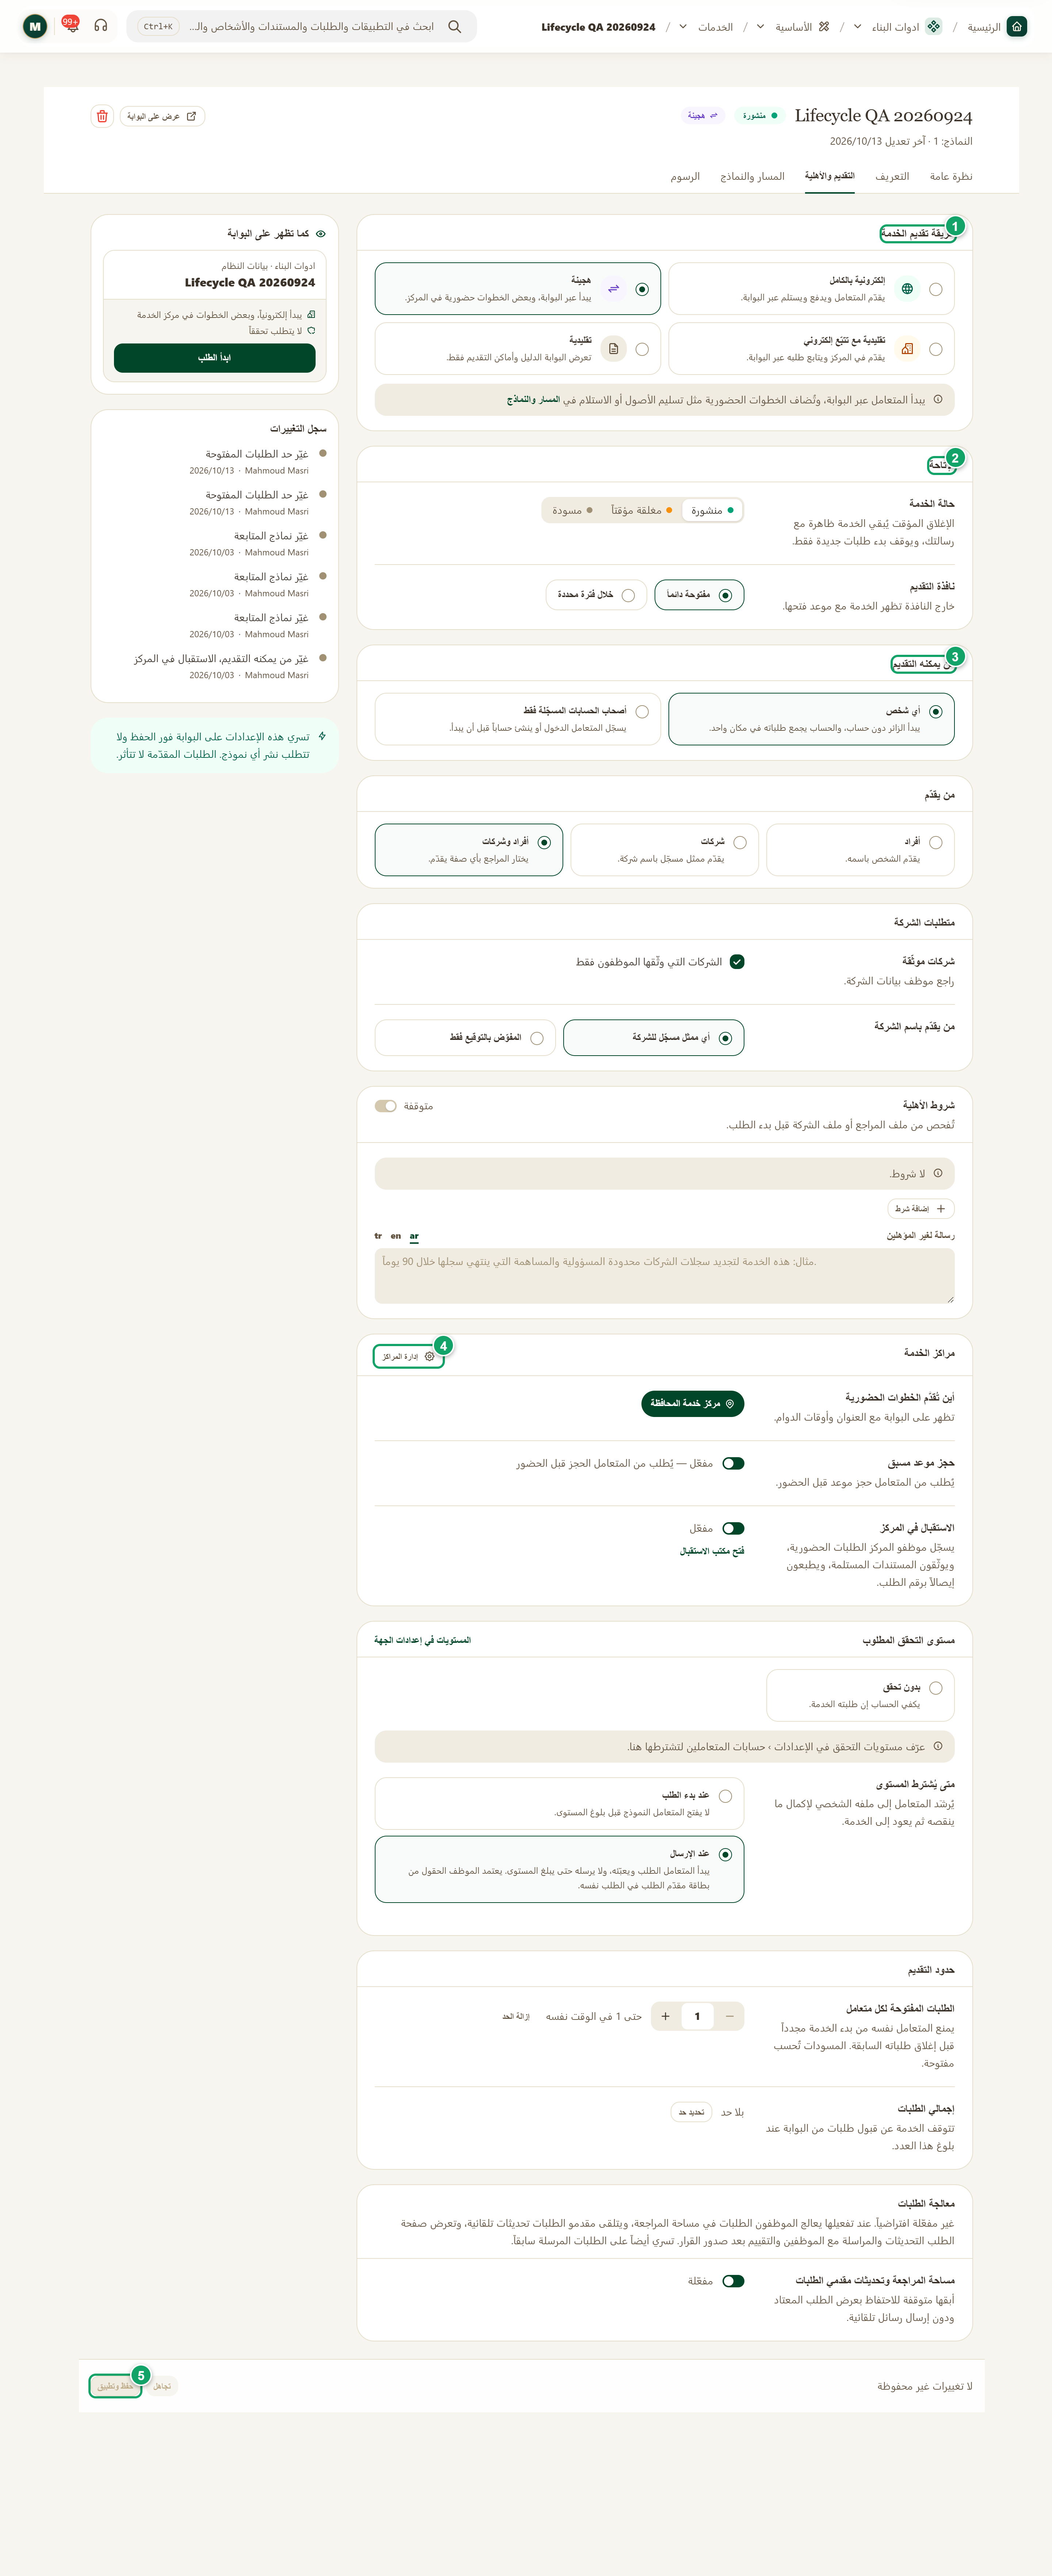
\includegraphics[width=0.95\linewidth,height=0.72\textheight,keepaspectratio]{figures/screens/ch06-services-delivery-ar.png}
\caption{تبويب «التقديم والأهلية» لخدمة هجينة}
\label{fig:builder-services-delivery-screen}
\shotnote{تعرض الصورة تبويب «التقديم والأهلية» لخدمة هجينة في مؤسسة الاختبار، لذلك يجمع أقسام الأهلية والتحقق التي تخص البدء عبر البوابة وأقسام المراكز والاستقبال التي تخص الخطوات الحضورية. وتبيّن أن الأقسام تُقرأ من الأعلى إلى الأسفل بالترتيب الذي تُضبط به، ثم تُحفظ معاً. ① «طريقة تقديم الخدمة»: الطرق الأربع، وهي التي تحدد الأقسام الظاهرة بعدها. ② «الإتاحة»: حالة الخدمة ونافذة التقديم. ③ «من يمكنه التقديم»: أي شخص أو أصحاب الحسابات المسجّلة فقط. ④ «إدارة المراكز»: يفتح نافذة «مراكز الخدمة». ⑤ «حفظ وتطبيق»: يطبّق الإعدادات على البوابة فوراً.}
\end{figure}

\begin{table}[H]
\centering
\caption{أقسام التقديم والإتاحة}
\label{tab:builder-services-delivery-parts}
\begin{tabularx}{\linewidth}{R{3.6cm} Y}
\rcHeaderRow
\thh{القسم} & \thh{ما تضبطه فيه}\\
طريقة تقديم الخدمة & إحدى الطرق الأربع. وإذا لم يناسب المسار الحالي الطريقة الجديدة، يظهر زر «تعديل المسار»، ولا تُطبَّق الطريقة إلا بعد حفظ المسار المعدّل.\\
الإتاحة & «حالة الخدمة»: «منشورة» أو «مغلقة مؤقتاً» مع «رسالة للمتعاملين» أو «مسودة». و«نافذة التقديم»: «مفتوحة دائماً» أو «خلال فترة محددة» بتاريخين.\\
من يمكنه التقديم & للخدمات التي تبدأ عبر البوابة: «أي شخص» دون حساب، أو «أصحاب الحسابات المسجّلة فقط».\\
مستوى التحقق المطلوب & للخدمات التي تبدأ عبر البوابة: «بدون تحقق» أو أحد المستويات المعرّفة في الإعدادات، ثم «متى يُشترط المستوى»: «عند بدء الطلب» أو «عند الإرسال».\\
حدود التقديم & «الطلبات المفتوحة لكل متعامل» حتى 9 طلبات، و«إجمالي الطلبات» الذي تتوقف الخدمة بعده عن قبول طلبات البوابة.\\
مراكز الخدمة وحجز موعد مسبق & للخدمات التي فيها خطوات حضورية: المراكز التي تجري فيها، وهل يُطلب من المتعامل «حجز موعد مسبق».\\
الاستقبال في المركز & يسمح لموظفي المركز بتسجيل الطلبات الحضورية وطباعة إيصال، ومنه رابط «فتح مكتب الاستقبال».\\
معالجة الطلبات & «مساحة المراجعة وتحديثات مقدمي الطلبات»: غير مفعّلة افتراضياً، وعند تفعيلها يعالج الموظفون الطلبات في مساحة المراجعة ويتلقى مقدمو الطلبات تحديثات تلقائية.\\
\end{tabularx}
\end{table}

\begin{table}[H]
\centering
\caption{أقسام الأهلية للخدمات التي تبدأ عبر البوابة}
\label{tab:builder-services-delivery-eligibility}
\begin{tabularx}{\linewidth}{R{3.6cm} Y}
\rcHeaderRow
\thh{القسم} & \thh{ما تضبطه فيه}\\
من يقدّم & «أفراد» أو «شركات» أو «أفراد وشركات». ويتطلب خيارا الشركات تفعيل ملفات الشركات من «إعدادات ملف الشركة».\\
متطلبات الشركة & «الشركات التي وثّقها الموظفون فقط»، و«من يقدّم باسم الشركة»: «أي ممثل مسجّل للشركة» أو «المفوّض بالتوقيع فقط».\\
شروط الأهلية & تفعّلها بـ«استخدام شروط الأهلية»، ثم تضيف بزر «إضافة شرط» شروطاً تُفحص من ملف المراجع أو ملف الشركة قبل بدء الطلب، مثل «العمر لا يقل عن». وتكتب «رسالة لغير المؤهلين».\\
\end{tabularx}
\end{table}

\begin{rcwarn}[مستوى يعتمده الموظف لا يُشترط عند البدء]
إذا تضمّن المستوى المختار حقلاً يعتمده الموظف من طلب قائم، واشترطته «عند بدء الطلب»، فلن يتمكن متعامل جديد من بدء الخدمة أبداً. لذلك يظهر تحذير مع زر «اشترطه عند الإرسال»، فاضغطه قبل الحفظ.
\end{rcwarn}

\begin{figure}[H]
\centering
\begin{tikzpicture}[node distance=0.5cm]
\node[stepBox] (a) {\RL{طريقة تقديم الخدمة}};
\node[stepBox,below=of a] (b) {\RL{الإتاحة}};
\node[stepBox,below=of b] (c) {\RL{من يقدّم وشروطه}};
\node[stepBox,below=of c] (d) {\RL{المراكز والاستقبال}};
\node[stepBox,below=of d] (e) {\RL{حفظ وتطبيق}};
\draw[flowsTo] (a) -- (b);
\draw[flowsTo] (b) -- (c);
\draw[flowsTo] (c) -- (d);
\draw[flowsTo] (d) -- (e);
\end{tikzpicture}
\rclegend
\caption{ضبط التقديم والأهلية}
\label{fig:builder-services-delivery-flow}
\shotnote{تأتي طريقة التقديم أولاً لأنها تحدد الأقسام التي تظهر بعدها: أقسام الأهلية والتحقق للخدمات التي تبدأ عبر البوابة، وأقسام المراكز والاستقبال للخدمات التي فيها خطوات حضورية. وتسري الإعدادات كلها على البوابة فور الحفظ، ولا تتأثر الطلبات المقدّمة قبلها.}
\end{figure}

\subsection{خطوات العمل والتحقق}
\begin{enumerate}
\item افتح الخدمة واضغط «التقديم والأهلية»، ثم تأكد من «طريقة تقديم الخدمة».
\item اختر في «الإتاحة» «حالة الخدمة» و«نافذة التقديم».
\item حدد «من يمكنه التقديم» و«من يقدّم»، وأضف «شروط الأهلية» إن احتجت إليها.
\item اختر مراكز الخدمة وفعّل «الاستقبال في المركز» إن كانت للخدمة خطوات حضورية، ثم اضبط «حدود التقديم».
\item اضغط «حفظ وتطبيق».
\end{enumerate}

\textbf{تحقق ومعالجة المشكلة:} تظهر رسالة «حُفظت — تسري على البوابة الآن»، وتتغير معاينة «كما تظهر على البوابة» بحسب اختياراتك. فإذا بقي زر الحفظ معطلاً بعد تغيير الطريقة، فاضغط «تعديل المسار» واحفظ المسار المناسب لها. وإذا ظهر «يجب أن تنتهي النافذة بعد بدايتها.»، فصحّح تاريخ «إلى».

\clearpage
\section{مراكز الخدمة}
\label{sec:builder-feature-services-centers}

مراكز الخدمة هي الأماكن التي يحضر إليها المتعاملون للخطوات الحضورية، مثل تسليم الأصول أو استلام النتيجة. وتُعرَّف المراكز مرة واحدة للمؤسسة كلها، ثم تختار كل خدمة منها ما يناسبها، فتظهر على البوابة مع العنوان وأوقات الدوام. ويحدد كل مركز أيضاً الموظفين الذين يفتح لهم مكتب الاستقبال عليه.

\textbf{المسار ومن يستخدمه:} «الخدمات» ← اضغط خدمة طريقتها ليست «إلكترونية بالكامل» ← «التقديم والأهلية» ← «إدارة المراكز». يضبطها مسؤول الخدمات عند افتتاح مركز أو تغيير دوامه أو موظفيه.

\begin{rcnote}[مثال: شركة الأفق]
يضيف مسؤول النظام بزر «إضافة مركز» ① مركزاً باسم «فرع حلب» ② وآخر باسم «المقر الرئيسي، دمشق» مع عنوان كل منهما وأوقات الدوام. ثم يضيف عمر حداد إلى «موظفو هذا المركز» ③ في فرع حلب، فيفتح مكتب الاستقبال لديه على هذا الفرع.
\end{rcnote}

\begin{figure}[H]
\centering
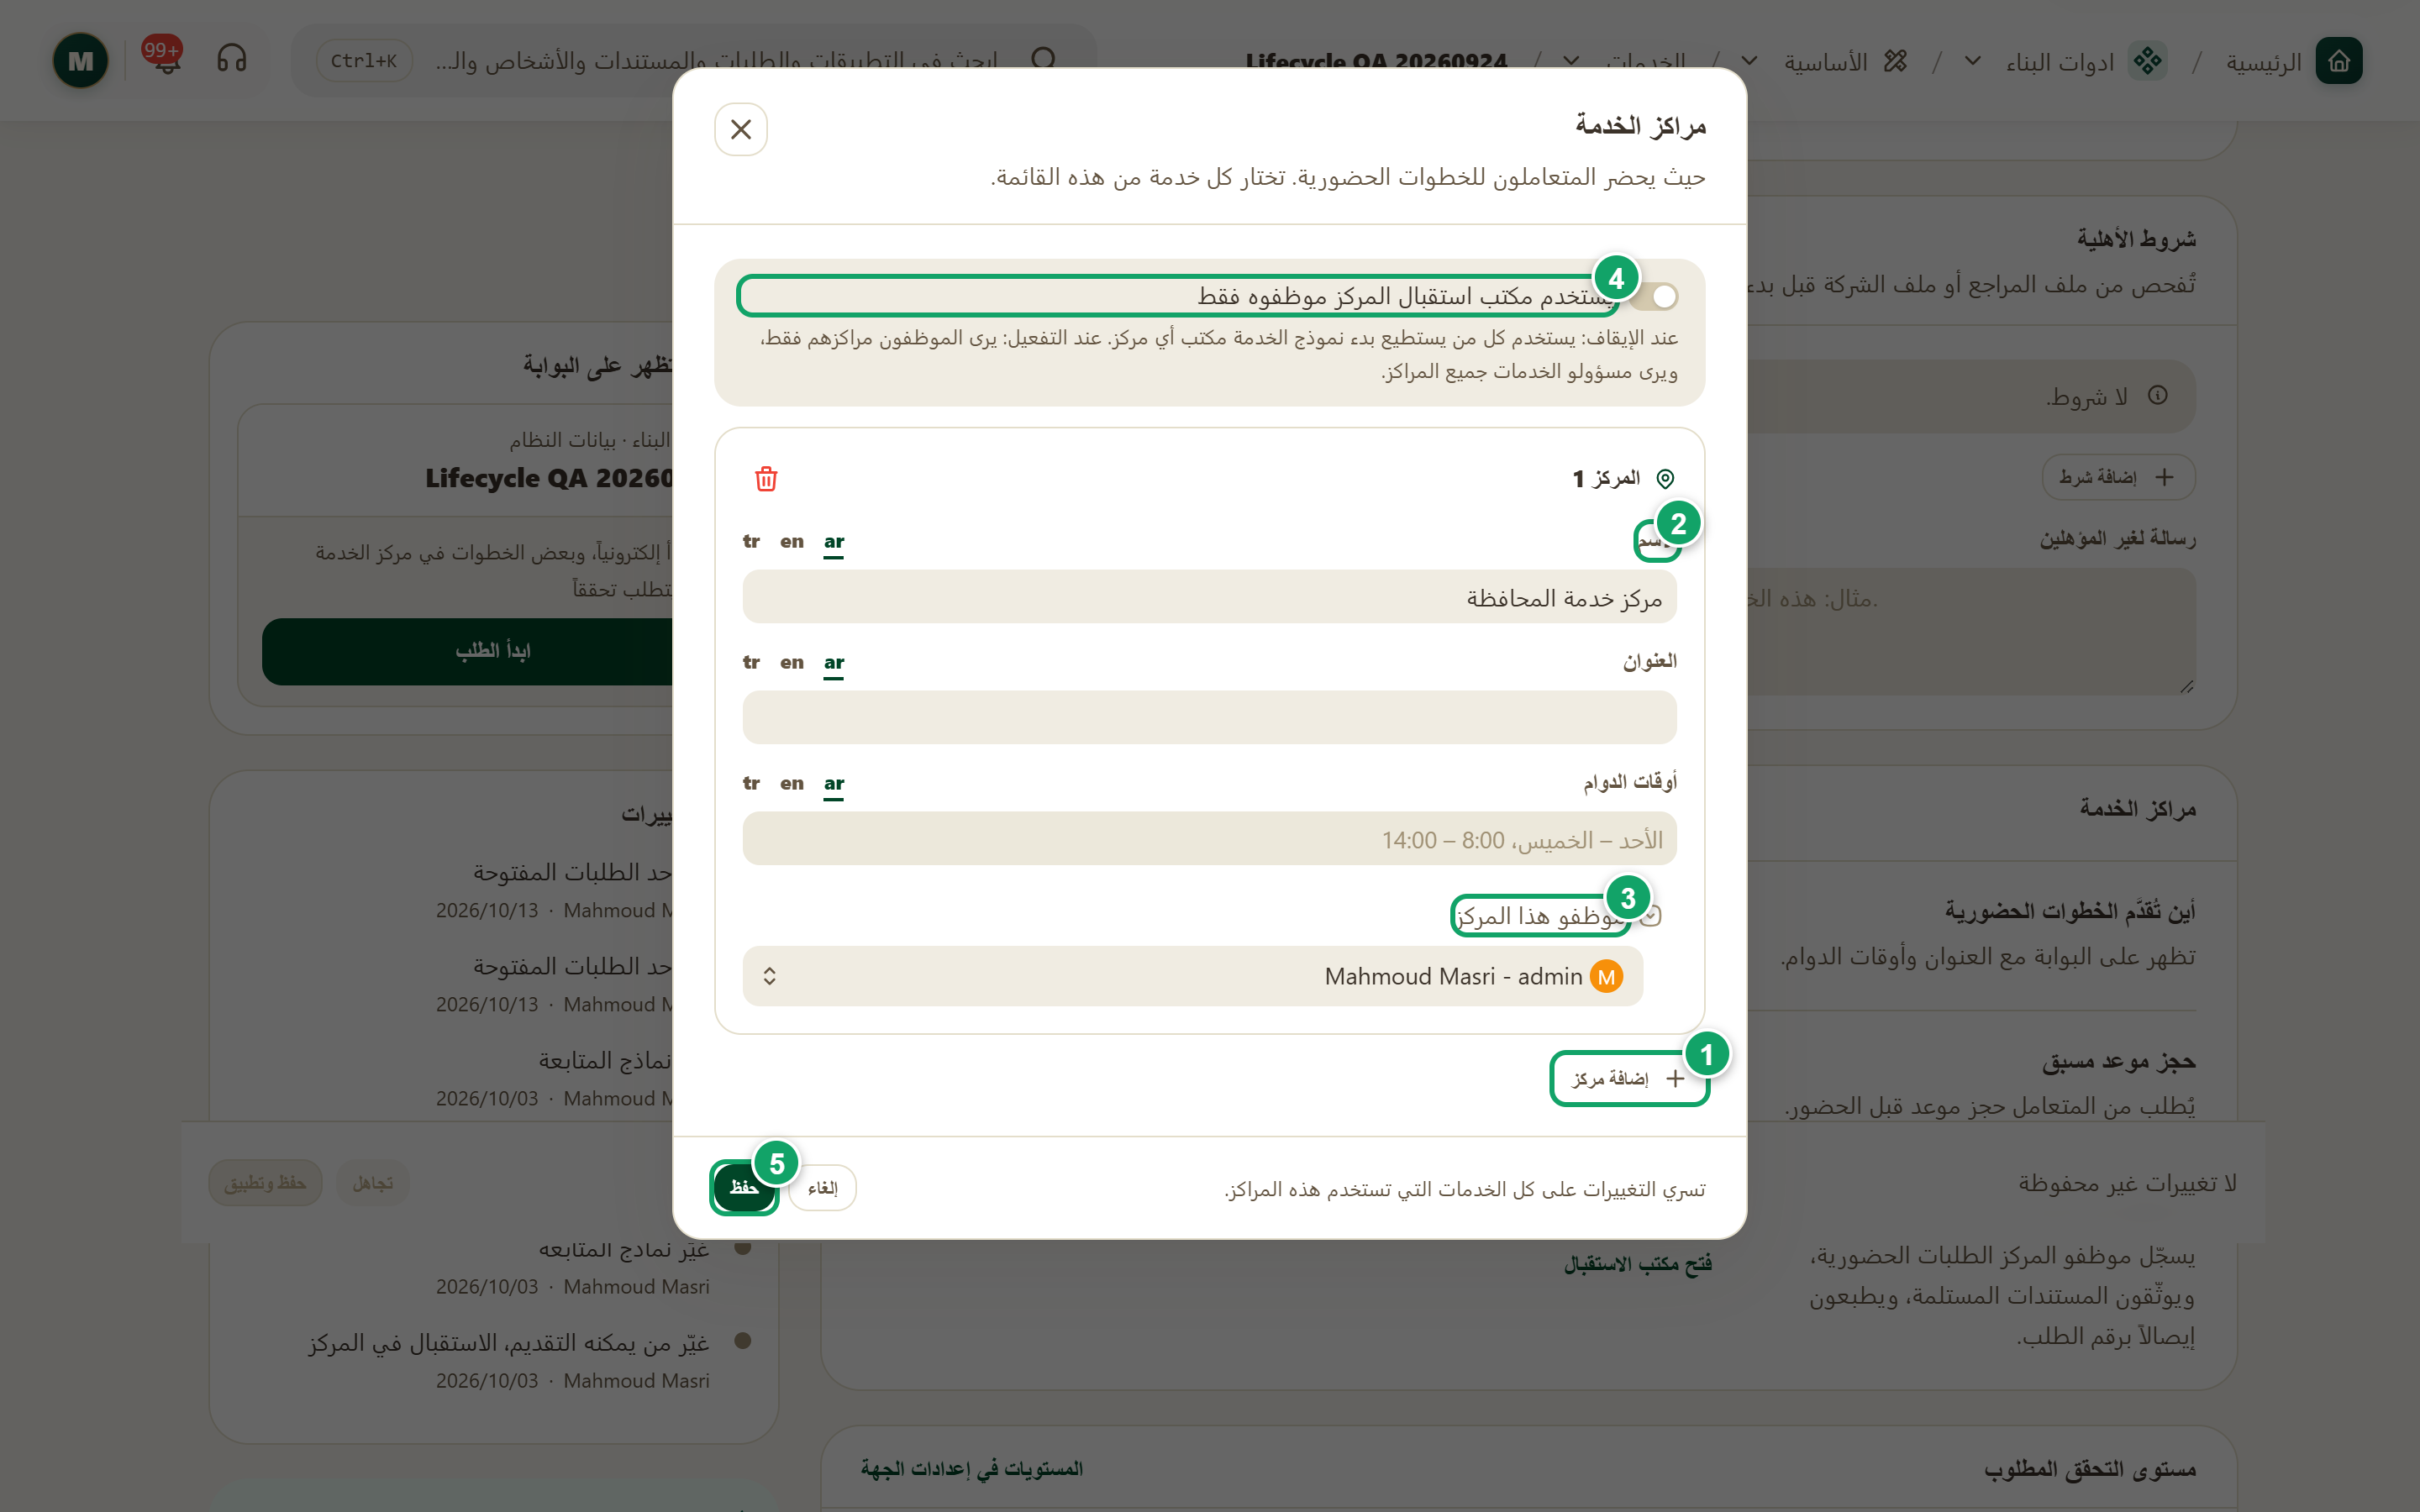
\includegraphics[width=0.95\linewidth,height=0.72\textheight,keepaspectratio]{figures/screens/ch06-services-centers-ar.png}
\caption{نافذة «مراكز الخدمة»}
\label{fig:builder-services-centers-screen}
\shotnote{تعرض الصورة نافذة «مراكز الخدمة» في مؤسسة الاختبار وفيها مركز واحد له اسم وأوقات دوام وموظف واحد. وتذكّرك العبارة أسفل النافذة بأن التغييرات تسري على كل الخدمات التي تستخدم هذه المراكز، لا على الخدمة المفتوحة وحدها. ① «إضافة مركز». ② «الاسم»: اسم المركز المطلوب كما يظهر للمتعاملين. ③ «موظفو هذا المركز»: من يفتح لهم مكتب الاستقبال على هذا المركز. ④ «يستخدم مكتب استقبال المركز موظفوه فقط»: يقصر مكتب كل مركز على موظفيه. ⑤ «حفظ»: يحفظ المراكز للمؤسسة كلها.}
\end{figure}

\begin{table}[H]
\centering
\caption{ما تضبطه في نافذة «مراكز الخدمة»}
\label{tab:builder-services-centers-parts}
\begin{tabularx}{\linewidth}{R{3.6cm} Y}
\rcHeaderRow
\thh{الحقل أو الخيار} & \thh{ما يعنيه}\\
الاسم & اسم المركز كما يظهر للمتعاملين، وهو مطلوب.\\
العنوان وأوقات الدوام & يظهران على البوابة، مثل «الأحد – الخميس، 8:00 – 14:00»، ويُطبع الدوام على إيصال الطلب الحضوري.\\
موظفو هذا المركز & الموظفون الذين يفتح مكتب الاستقبال لديهم على هذا المركز.\\
يستخدم مكتب استقبال المركز موظفوه فقط & عند الإيقاف يستخدم كل من يستطيع بدء نموذج الخدمة مكتب أي مركز. وعند التفعيل يرى الموظفون مراكزهم فقط، ويرى مسؤولو الخدمات جميع المراكز.\\
\end{tabularx}
\end{table}

\begin{rcwarn}[التغيير يشمل كل الخدمات]
تسري تغييرات المراكز على كل الخدمات التي تستخدمها، لذلك لا تحذف مركزاً أو تغيّر دوامه إلا بعد التأكد من الخدمات المرتبطة به.
\end{rcwarn}

\begin{figure}[H]
\centering
\begin{tikzpicture}[node distance=0.5cm]
\node[stepBox] (a) {\RL{إدارة المراكز}};
\node[stepBox,below=of a] (b) {\RL{إضافة مركز وبياناته}};
\node[stepBox,below=of b] (c) {\RL{تحديد موظفي المركز}};
\node[stepBox,below=of c] (d) {\RL{اختياره في الخدمة}};
\node[stepBox,below=of d] (e) {\RL{حفظ وتطبيق}};
\draw[flowsTo] (a) -- (b);
\draw[flowsTo] (b) -- (c);
\draw[flowsTo] (c) -- (d);
\draw[flowsTo] (d) -- (e);
\end{tikzpicture}
\rclegend
\caption{إعداد مركز خدمة وربطه بالخدمة}
\label{fig:builder-services-centers-flow}
\shotnote{يفصل المخطط بين خطوتين تُحفظ كل منهما وحدها: النافذة تحفظ المراكز للمؤسسة كلها بزر «حفظ»، ثم تختار الخدمة مراكزها وتحفظها بزر «حفظ وتطبيق». فإنشاء المركز وحده لا يجعله ظاهراً في خدمة بعينها.}
\end{figure}

\subsection{خطوات العمل والتحقق}
\begin{enumerate}
\item افتح «التقديم والأهلية» في خدمة لها خطوات حضورية، واضغط «إدارة المراكز».
\item اضغط «إضافة مركز»، واكتب «الاسم» و«العنوان» و«أوقات الدوام».
\item اختر «موظفو هذا المركز»، وقرّر هل تفعّل «يستخدم مكتب استقبال المركز موظفوه فقط»، ثم اضغط «حفظ».
\item اختر المركز في «أين تُقدَّم الخطوات الحضورية»، ثم اضغط «حفظ وتطبيق».
\end{enumerate}

\textbf{تحقق ومعالجة المشكلة:} يظهر المركز في معاينة «كما تظهر على البوابة» وفي بطاقة «مراكز الخدمة» في «نظرة عامة». وإذا ظهر للموظف في مكتب الاستقبال «لست ضمن موظفي أي مركز خدمة»، فأضفه إلى «موظفو هذا المركز». وإذا لم يُحفظ المركز، فتحقق من أن لكل مركز اسماً.

\clearpage
\section{المسار والنماذج}
\label{sec:builder-feature-services-path}

يرسم تبويب «المسار والنماذج» ما يمر به الطلب بالترتيب: خطوة البدء، ثم الخطوات التالية، وأين تجري كل منها. فقد تكون الخطوة نموذجاً يعبّئه المتعامل عبر البوابة، أو خطوة حضورية في المركز يوثّقها الموظف. ويضم التبويب أيضاً النماذج التي يبدؤها المتعامل في أي وقت خارج المسار، ونماذج المتابعة التي تُطلب منه عند حالة معينة.

\textbf{المسار ومن يستخدمه:} «الخدمات» ← اضغط الخدمة ← «المسار والنماذج». يبنيه مسؤول الخدمة بعد نشر النماذج التي سيستخدمها.

\begin{rcnote}[مثال: شركة الأفق]
يبدأ مسار «طلب زيارة فرع» بنموذج الطلب عبر البوابة، ثم يضيف مسؤول النظام بزر «إضافة خطوة» ① خطوة حضورية باسم «حضور الزيارة» ② تُتاح عندما يكون الطلب «مقبول». ويفعّل لها «يتطلب موعداً»، فتظهر عليها شارة «بموعد».
\end{rcnote}

\begin{figure}[H]
\centering
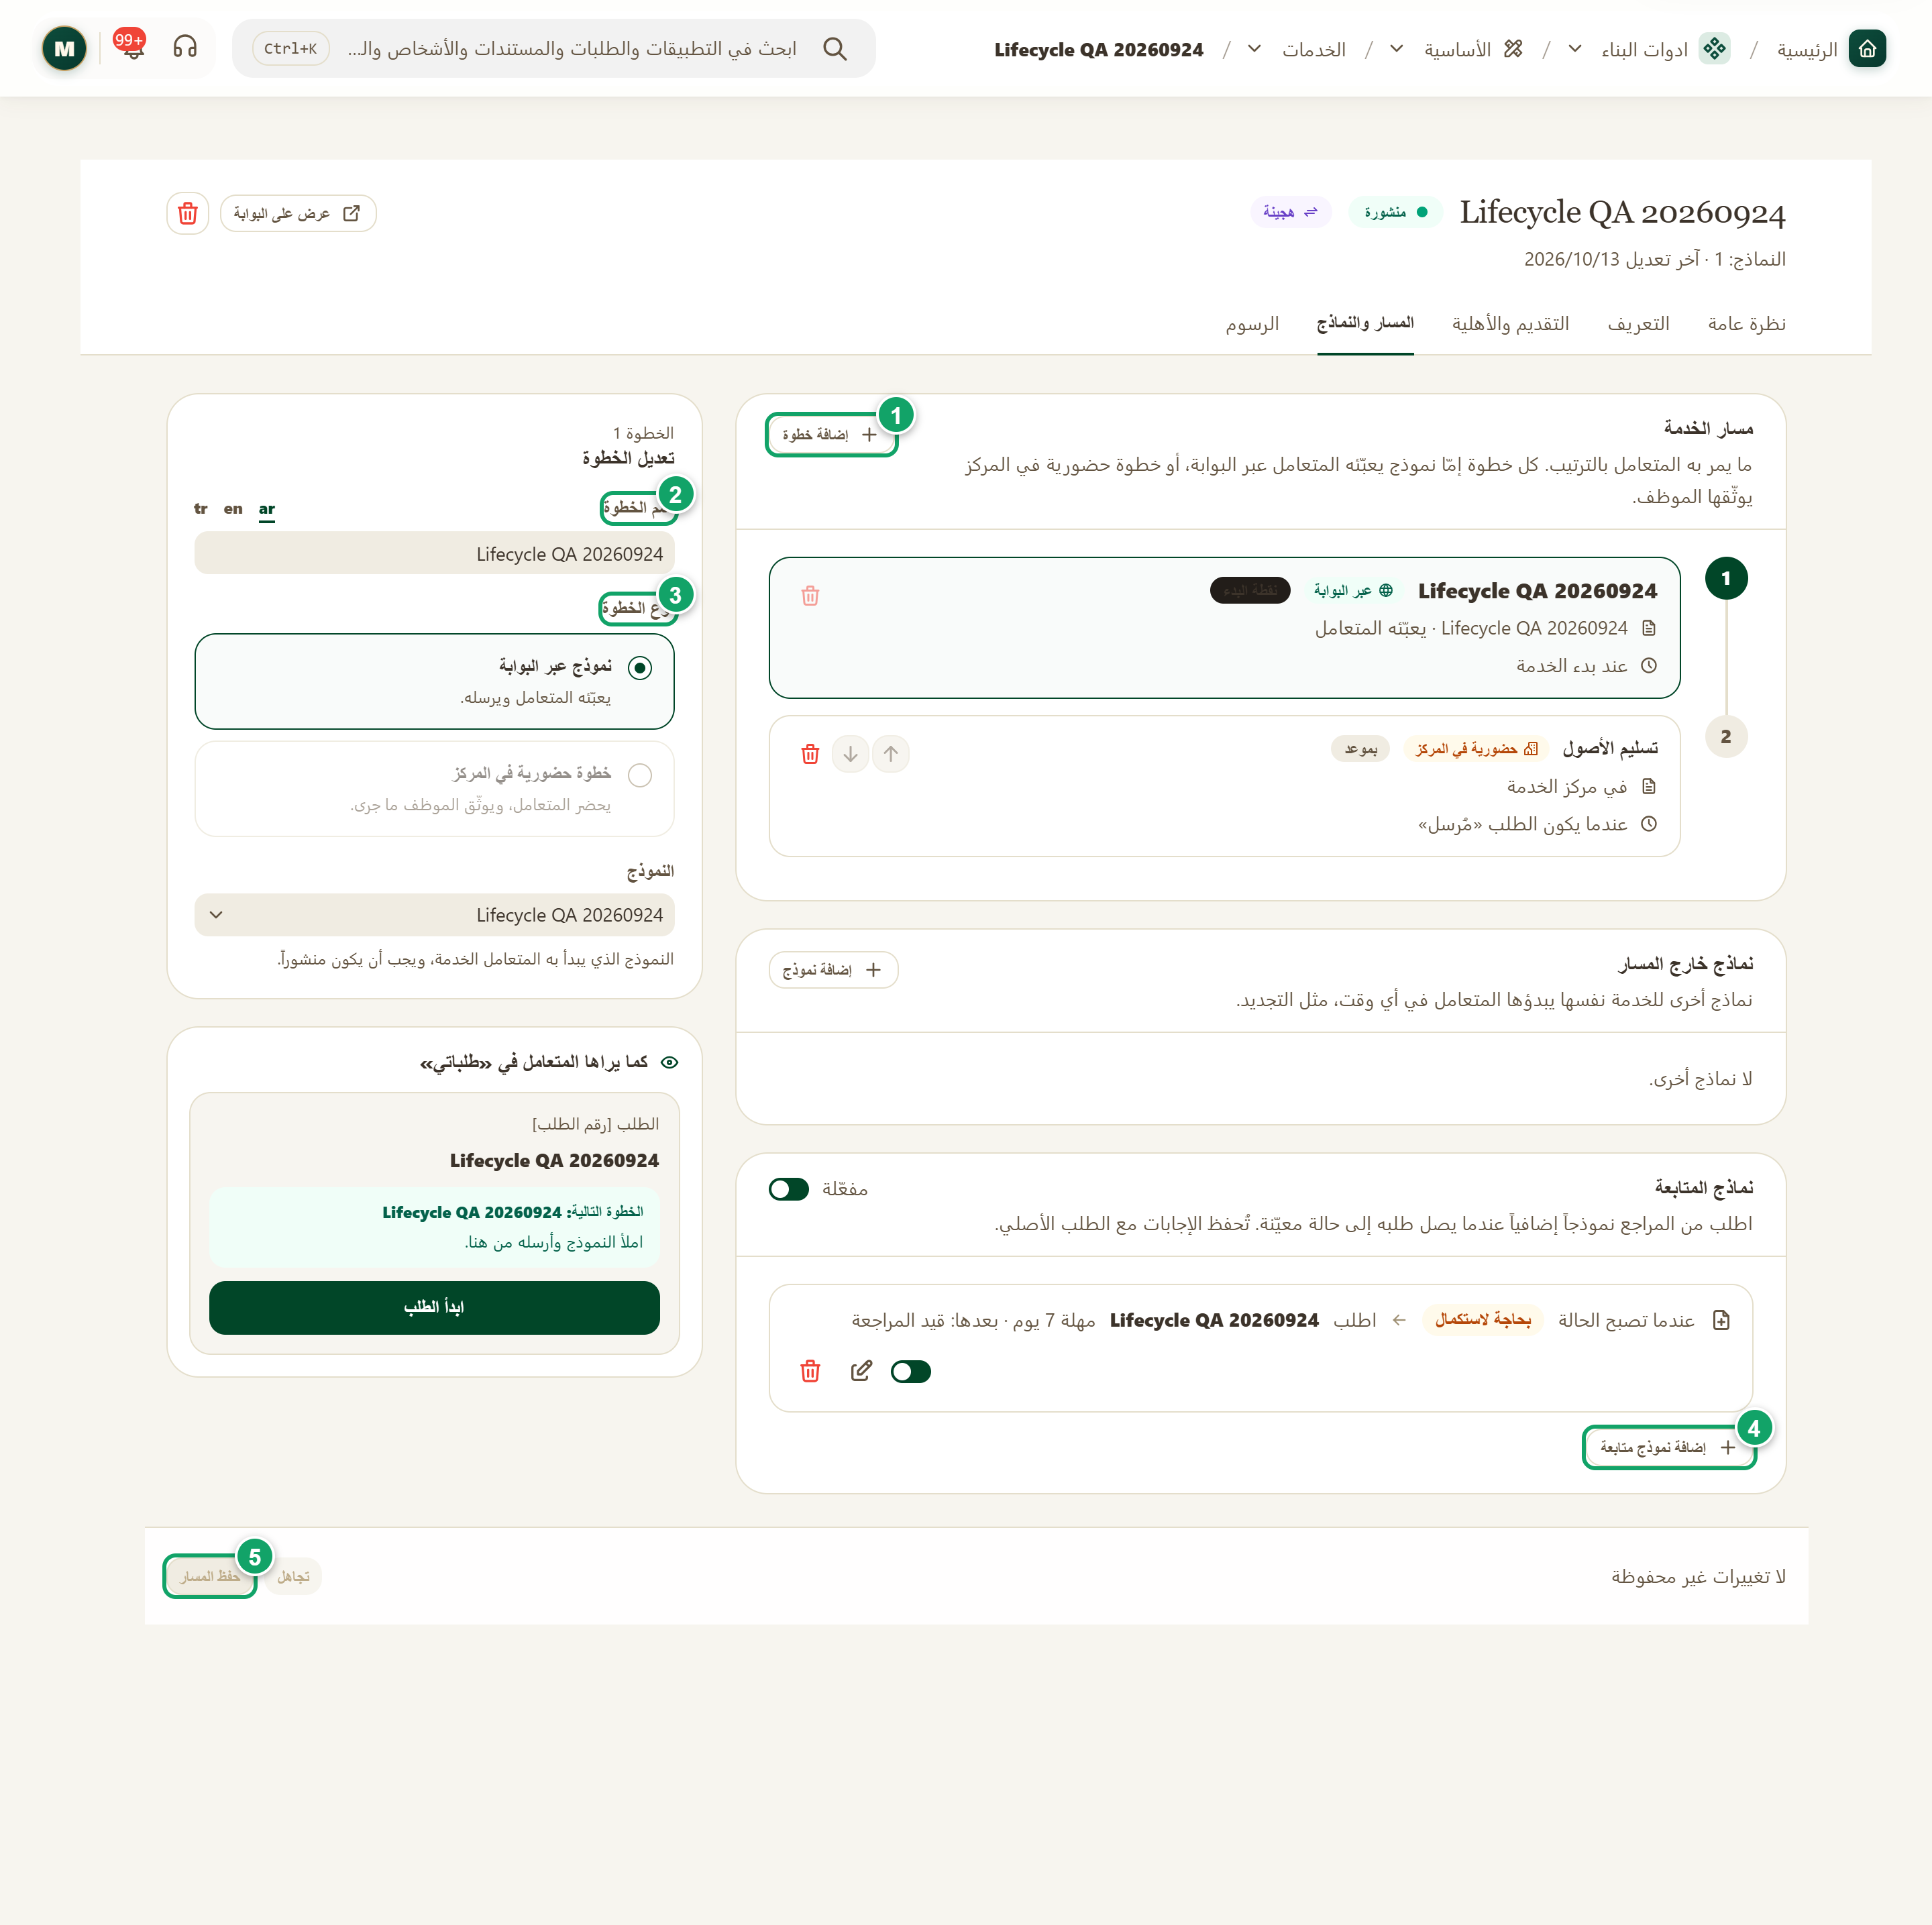
\includegraphics[width=0.95\linewidth,height=0.72\textheight,keepaspectratio]{figures/screens/ch06-services-path-ar.png}
\caption{تبويب «المسار والنماذج»}
\label{fig:builder-services-path-screen}
\shotnote{تعرض الصورة مسار خدمة هجينة في مؤسسة الاختبار: خطوة البدء عبر البوابة بشارة «نقطة البدء»، ثم خطوة حضورية «بموعد»، ومعهما قاعدة متابعة واحدة. وتبيّن أن الخطوة المختارة تُعدَّل في اللوحة الجانبية، وأن خيار الخطوة الحضورية معطّل لخطوة البدء في هذه الطريقة. ① «إضافة خطوة»: يضيف خطوة في آخر المسار. ② «اسم الخطوة»: الاسم الذي يراه المتعامل في «طلباتي». ③ «نوع الخطوة»: نموذج عبر البوابة أو خطوة حضورية في المركز. ④ «إضافة نموذج متابعة»: يضيف قاعدة تطلب نموذجاً عند حالة معينة. ⑤ «حفظ المسار».}
\end{figure}

\begin{table}[H]
\centering
\caption{إعدادات الخطوة}
\label{tab:builder-services-path-step}
\begin{tabularx}{\linewidth}{R{3.6cm} Y}
\rcHeaderRow
\thh{الإعداد} & \thh{ما يعنيه}\\
اسم الخطوة & الاسم الذي يراه المتعامل في «طلباتي»، مثل «الخطوة التالية: …».\\
نوع الخطوة & «نموذج عبر البوابة» يعبّئه المتعامل ويرسله، أو «خطوة حضورية في المركز» يحضر لها المتعامل ويوثّق الموظف ما جرى.\\
النموذج أو محضر الموظف & لخطوة البوابة نموذج منشور، ويمكن تركه فارغاً إذا استُكملت الخطوة في الطلب نفسه. وللخطوة الحضورية «محضر الموظف (اختياري)».\\
متى تُتاح & «بعد الخطوة السابقة»، أو عندما يصل الطلب إلى حالة من حالات نموذج البدء.\\
يتطلب موعداً & للخطوات الحضورية، ويعني أن يحجز المتعامل موعداً في أحد مراكز الخدمة.\\
\end{tabularx}
\end{table}

وتحمل الخطوة الأولى شارة «نقطة البدء»، ولا يمكن حذفها في الخدمات التي تبدأ عبر البوابة. وتضم الخدمة حتى 20 خطوة، ولا يتكرر النموذج فيها. أما الخدمة «إلكترونية بالكامل» فلا تضم خطوات حضورية، والخدمة التقليدية تبدأ خطوتها الأولى في المركز.

\begin{table}[H]
\centering
\caption{أقسام التبويب الأخرى}
\label{tab:builder-services-path-more}
\begin{tabularx}{\linewidth}{R{3.6cm} Y}
\rcHeaderRow
\thh{القسم} & \thh{ما يقدمه}\\
نماذج خارج المسار & للخدمات التي تبدأ عبر البوابة: نماذج منشورة يبدؤها المتعامل في أي وقت، مثل التجديد، وتضيفها بزر «إضافة نموذج».\\
نماذج المتابعة & تفعّلها بـ«استخدام نماذج المتابعة»، ثم تضيف قاعدة: «الحالة التي تطلب النموذج»، و«النموذج»، و«أيام لتعبئته»، و«بعد إرسال المراجع انقل الطلب إلى»، و«أبلغ المراجع». وتُحفظ الإجابات مع الطلب الأصلي.\\
كما يراها المتعامل في «طلباتي» & معاينة للخطوة المختارة كما تظهر للمتعامل في طلبه.\\
\end{tabularx}
\end{table}

\begin{figure}[H]
\centering
\begin{tikzpicture}[node distance=0.5cm]
\node[stepBox] (a) {\RL{نقطة البدء}};
\node[stepBox,below=of a] (b) {\RL{إضافة خطوة}};
\node[stepBox,below=of b] (c) {\RL{نوع الخطوة ونموذجها}};
\node[stepBox,below=of c] (d) {\RL{متى تُتاح}};
\node[stepBox,below=of d] (e) {\RL{حفظ المسار}};
\draw[flowsTo] (a) -- (b);
\draw[flowsTo] (b) -- (c);
\draw[flowsTo] (c) -- (d);
\draw[flowsTo] (d) -- (e);
\end{tikzpicture}
\rclegend
\caption{بناء مسار الخدمة}
\label{fig:builder-services-path-flow}
\shotnote{يبدأ المسار دائماً من نقطة البدء التي حُددت عند إنشاء الخدمة، ثم تُضاف الخطوات بعدها واحدة واحدة. وتعتمد خطوة «متى تُتاح» على حالات نموذج البدء، لذلك اضبط دورة حياته قبل أن تبني مساراً ينتظر حالة معينة.}
\end{figure}

\subsection{خطوات العمل والتحقق}
\begin{enumerate}
\item افتح الخدمة واضغط «المسار والنماذج»، وراجع خطوة «نقطة البدء».
\item اضغط «إضافة خطوة»، واكتب «اسم الخطوة» واختر «نوع الخطوة».
\item اختر «النموذج» أو «محضر الموظف (اختياري)»، ثم حدد «متى تُتاح»، وفعّل «يتطلب موعداً» إن لزم.
\item رتّب الخطوات بزرّي «نقل للأعلى» و«نقل للأسفل»، وأضف نماذج المتابعة إن احتجت إليها.
\item اضغط «حفظ المسار».
\end{enumerate}

\textbf{تحقق ومعالجة المشكلة:} يتحول شريط الحفظ إلى «لا تغييرات غير محفوظة»، ويظهر عدد الخطوات في «جاهزية الخدمة». فإذا عُطّل الحفظ وظهرت رسالة مثل «الخدمة الإلكترونية بالكامل لا تضم خطوات حضورية.»، فغيّر نوع الخطوة أو طريقة التقديم. وإذا ظهر «لا حالات لنموذج البدء بعد»، فأضف الحالات من «دورة الحياة» في النموذج.

\clearpage
\section{الرسوم}
\label{sec:builder-feature-services-fees}

يحوّل تبويب «الرسوم» كلفة الخدمة إلى بنود واضحة، فتعرضها البوابة للمتعامل قبل أن يبدأ، ويعرف كل طلب ما عليه ومتى يُستحق. ويمكن أن يتوقف البند على إجابة في النموذج، وأن يُعفى منه من يقدّم إثباتاً. ويحدد التبويب أيضاً ما يحدث للطلب عندما يُستحق رسم، ومهلة السداد.

\textbf{المسار ومن يستخدمه:} «الخدمات» ← اضغط الخدمة ← «الرسوم». يضبطه من يبني الخدمة بالتنسيق مع المسؤول المالي.

\begin{rcnote}[مثال: شركة الأفق]
يفعّل مسؤول النظام «استخدام بنود الرسوم»، ويضيف بزر «إضافة بند» ① بنداً باسم «رسم الزيارة» يُستحق «عند زيارة المركز». فيرى العميل الرسم على صفحة الخدمة، ويسجّل عمر حداد رقم الإيصال عند استلامه في فرع حلب.
\end{rcnote}

\begin{figure}[H]
\centering
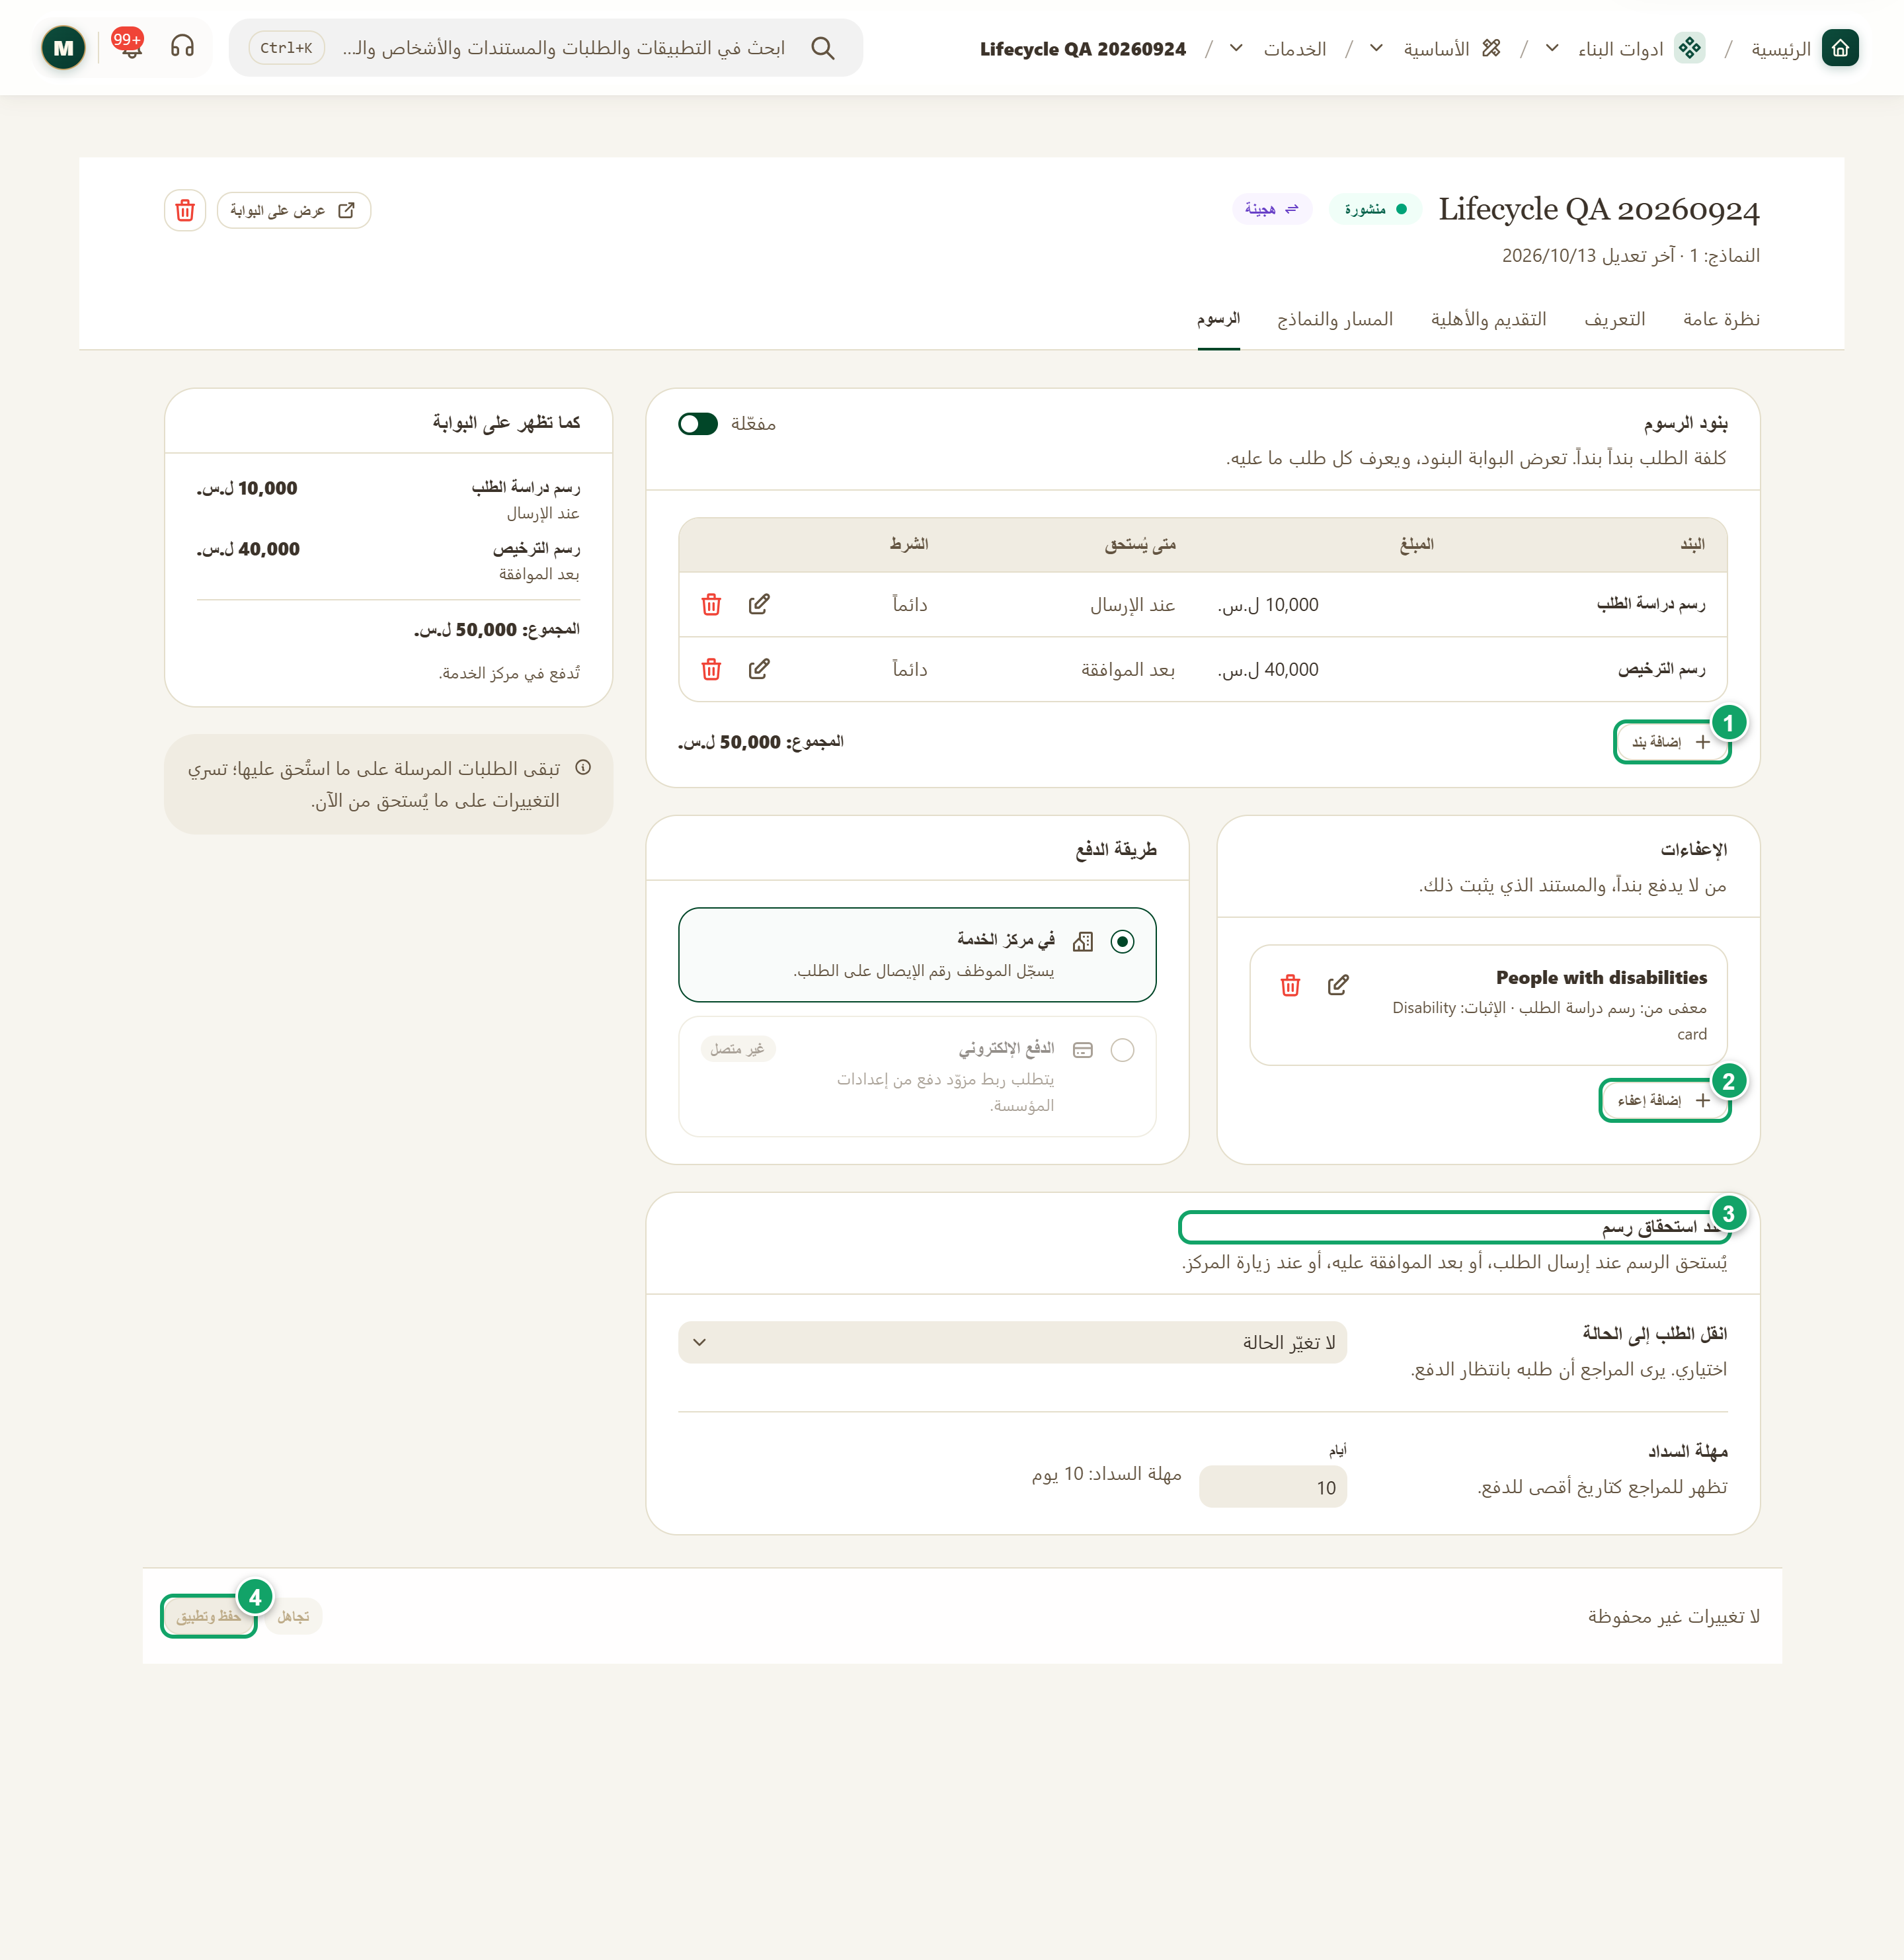
\includegraphics[width=0.95\linewidth,height=0.72\textheight,keepaspectratio]{figures/screens/ch06-services-fees-ar.png}
\caption{تبويب «الرسوم»}
\label{fig:builder-services-fees-screen}
\shotnote{تعرض الصورة رسوم خدمة في مؤسسة الاختبار: بندان بمبلغيهما ووقت استحقاق كل منهما، وإعفاء واحد، والدفع في مركز الخدمة لأن الدفع الإلكتروني «غير متصل». وتوضح المعاينة الجانبية المجموع كما يراه المتعامل، فتراجع أثر كل تغيير قبل حفظه. ① «إضافة بند». ② «إضافة إعفاء»: يضيف فئة معفاة من بند موجود. ③ «عند استحقاق رسم»: الحالة التي ينتقل إليها الطلب ومهلة السداد. ④ «حفظ وتطبيق»: يحفظ الرسوم وتسري على ما يُستحق من الآن.}
\end{figure}

\begin{table}[H]
\centering
\caption{أعمدة «بنود الرسوم»}
\label{tab:builder-services-fees-items}
\begin{tabularx}{\linewidth}{R{3.6cm} Y}
\rcHeaderRow
\thh{العمود} & \thh{ما يعنيه}\\
البند & اسم الرسم، مثل «رسم الترخيص»، وهو مطلوب.\\
المبلغ & قيمة البند بعملة الخدمة، وهو مطلوب.\\
متى يُستحق & «عند الإرسال» أو «بعد الموافقة» أو «عند زيارة المركز».\\
الشرط & «دائماً»، أو شرط يطبّق البند مع إجابات معينة في حقل اختيار من النموذج، وتختارها في «الإجابات التي يُطبَّق معها البند».\\
\end{tabularx}
\end{table}

\begin{table}[H]
\centering
\caption{بقية أقسام «الرسوم»}
\label{tab:builder-services-fees-more}
\begin{tabularx}{\linewidth}{R{3.6cm} Y}
\rcHeaderRow
\thh{القسم} & \thh{ما يقدمه}\\
الإعفاءات & «المعفَون» و«معفى من» و«الإثبات»، وخيار «يوافق الموظف على الإعفاء» إذا كان المراجِع يمنحه بعد التحقق من المستند.\\
طريقة الدفع & «في مركز الخدمة» حيث يسجّل الموظف رقم الإيصال على الطلب. أما «الدفع الإلكتروني» فيظهر «غير متصل» حتى يُربط مزوّد دفع.\\
عند استحقاق رسم & «انقل الطلب إلى الحالة» ليرى المراجع أن طلبه بانتظار الدفع، و«مهلة السداد» بالأيام.\\
كما تظهر على البوابة & معاينة البنود والمجموع كما يراها المتعامل.\\
\end{tabularx}
\end{table}

\begin{figure}[H]
\centering
\begin{tikzpicture}[node distance=0.5cm]
\node[stepBox] (a) {\RL{استخدام بنود الرسوم}};
\node[stepBox,below=of a] (b) {\RL{إضافة البنود}};
\node[stepBox,below=of b] (c) {\RL{الإعفاءات}};
\node[stepBox,below=of c] (d) {\RL{عند استحقاق رسم}};
\node[stepBox,below=of d] (e) {\RL{حفظ وتطبيق}};
\draw[flowsTo] (a) -- (b);
\draw[flowsTo] (b) -- (c);
\draw[flowsTo] (c) -- (d);
\draw[flowsTo] (d) -- (e);
\end{tikzpicture}
\rclegend
\caption{إعداد رسوم الخدمة}
\label{fig:builder-services-fees-flow}
\shotnote{تأتي البنود قبل الإعفاءات لأن الإعفاء يشير إلى بنود موجودة، ولا يمكن إضافته قبلها. وتبقى الطلبات المرسلة على ما استُحق عليها، أما التغييرات فتسري على ما يُستحق من الآن.}
\end{figure}

\subsection{خطوات العمل والتحقق}
\begin{enumerate}
\item افتح الخدمة واضغط «الرسوم»، ثم فعّل «استخدام بنود الرسوم».
\item اضغط «إضافة بند»، واكتب «اسم البند» والمبلغ، واختر متى يُستحق وشرطه، ثم اضغط «تم».
\item أضف الإعفاءات بزر «إضافة إعفاء» إن وُجدت.
\item اختر في «عند استحقاق رسم» الحالة التي ينتقل إليها الطلب و«مهلة السداد».
\item اضغط «حفظ وتطبيق»، وراجع المجموع في «كما تظهر على البوابة».
\end{enumerate}

\textbf{تحقق ومعالجة المشكلة:} يظهر عدد البنود في بند «الرسوم» من «جاهزية الخدمة». فإذا بقي الحفظ معطلاً، فاقرأ «يحتاج كل بند إلى اسم ومبلغ.» وأكمل البند الناقص. وإذا عُطّل «إضافة إعفاء»، فأضف بنداً واحداً على الأقل أولاً.

\clearpage
\section{إتاحة نموذج على البوابة}
\label{sec:builder-feature-services-publish}

قد يكون لديك نموذج داخلي منشور تريد أن يصل إلى المتعاملين. فبدلاً من إنشاء خدمة من الصفر، يحوّله زر «إتاحته على البوابة» في خطوة واحدة إلى خدمة جديدة، أو يضيفه خطوةً إلى خدمة قائمة. وتبدأ الخدمة الجديدة بإعدادات المؤسسة الافتراضية، ثم تغيّرها من صفحة الخدمة متى شئت دون إعادة نشر النموذج.

\textbf{المسار ومن يستخدمه:} «الخدمات» ← «نماذج داخلية» ← «إتاحته على البوابة»، أو من تبويب «الخدمة» في إعدادات النموذج. يستخدمه مسؤول الخدمات عندما يصبح نموذج داخلي خدمةً للجمهور.

\begin{rcnote}[مثال: شركة الأفق]
تملك الأفق نموذجاً داخلياً منشوراً لتجديد طلب الزيارة، فيضغط مسؤول النظام «إتاحته على البوابة» ويختار «خطوة في خدمة قائمة». ثم يختار خدمة «طلب زيارة فرع» ويضيفه بصفة «نموذج خارج المسار»، فيبدؤه العميل في أي وقت.
\end{rcnote}

\begin{table}[H]
\centering
\caption{خيارات نافذة الإتاحة}
\label{tab:builder-services-publish-options}
\begin{tabularx}{\linewidth}{R{3.6cm} Y}
\rcHeaderRow
\thh{الخيار} & \thh{ما يعنيه}\\
خدمة جديدة & الحالة الأبسط: خدمة واحدة لهذا النموذج. وتكتب «اسم الخدمة على البوابة».\\
من يعبّئ هذا النموذج & «المتعامل عبر البوابة» فتُنشأ الخدمة «إلكترونية بالكامل»، أو «الموظف في المركز» فتُنشأ «تقليدية مع تتبّع إلكتروني».\\
انشر الخدمة على البوابة الآن & عند تحديده يصبح الزر «إنشاء الخدمة ونشرها»، وعند إلغائه يصبح «إنشاء الخدمة كمسودة».\\
خطوة في خدمة قائمة & تختار «الخدمة» من الخدمات التي تبدأ إلكترونياً، ثم «يُضاف كـ»: «نموذج خارج المسار» أو «خطوة في المسار»، وتضغط «إضافة إلى الخدمة».\\
\end{tabularx}
\end{table}

وتظهر في الخدمة الجديدة إعدادات افتراضية: يقدّم أي شخص، بدون مستوى تحقق، مفتوحة دائماً، بلا حدود. أما النموذج المضاف إلى خدمة قائمة فيتبع أهليتها ومستوى التحقق فيها. وتجد في قائمة الخدمات أحياناً نموذجاً بشارة «من إعدادات النموذج»، وهو منشور للعامة بإعداداته القديمة؛ فاضغط «إنشاء خدمة» لتديره كبقية الخدمات.

\begin{figure}[H]
\centering
\begin{tikzpicture}[node distance=0.5cm]
\node[stepBox] (a) {\RL{نشر النموذج في المنشئ}};
\node[stepBox,below=of a] (b) {\RL{إتاحته على البوابة}};
\node[stepBox,below=of b] (c) {\RL{خدمة جديدة أو قائمة}};
\node[stepBox,below=of c] (d) {\RL{الإنشاء أو الإضافة}};
\node[stepBox,below=of d] (e) {\RL{مراجعة صفحة الخدمة}};
\draw[flowsTo] (a) -- (b);
\draw[flowsTo] (b) -- (c);
\draw[flowsTo] (c) -- (d);
\draw[flowsTo] (d) -- (e);
\end{tikzpicture}
\rclegend
\caption{تحويل نموذج داخلي إلى خدمة}
\label{fig:builder-services-publish-flow}
\shotnote{يبدأ المخطط بنشر النموذج لأن زر الإتاحة يبقى معطلاً حتى ذلك الحين. وينتهي بصفحة الخدمة لأن الإعدادات الافتراضية تناسب البداية فقط، فراجع الأهلية والدليل قبل أن تعتمد الخدمة.}
\end{figure}

\subsection{خطوات العمل والتحقق}
\begin{enumerate}
\item افتح «الخدمات» وابحث عن النموذج في «نماذج داخلية».
\item اضغط «إتاحته على البوابة»، واختر «خدمة جديدة» أو «خطوة في خدمة قائمة».
\item للخدمة الجديدة: اكتب الاسم واختر «من يعبّئ هذا النموذج»، وقرّر هل تحدد «انشر الخدمة على البوابة الآن».
\item للخدمة القائمة: اختر «الخدمة» و«يُضاف كـ»، ثم اضغط «إضافة إلى الخدمة».
\end{enumerate}

\textbf{تحقق ومعالجة المشكلة:} تُفتح صفحة الخدمة مباشرة، ويختفي النموذج من «نماذج داخلية». فإذا كان الزر معطلاً مع التلميح «انشر النموذج في المنشئ أولاً»، فانشر النموذج ثم عُد. وإذا ظهر «لا توجد خدمات تبدأ إلكترونياً بعد»، فأنشئ خدمة جديدة بدلاً من الإضافة.

\clearpage
\section{الخدمة في إعدادات النموذج}
\label{sec:builder-feature-services-form-settings}

لا تحتاج إلى مغادرة منشئ النماذج لتعرف علاقة النموذج بالخدمات. ففي إعدادات النموذج تبويب «الخدمة» يبيّن الخدمة التي ينتمي إليها النموذج ودوره فيها، وما تحدده الخدمة له، وهل يتوافق معها. ويذكّرك التبويب بقاعدة مهمة: إعدادات الخدمة تسري فوراً من صفحتها، أما تغييرات النموذج فتسري بعد نشره.

\textbf{المسار ومن يستخدمه:} «النماذج» ← افتح النموذج ← «الإعدادات» ← «الخدمة» في نافذة «إعدادات النموذج». يستخدمه من يعدّل النموذج ليتأكد من أن تعديله لا يكسر مسار الخدمة.

\begin{rcnote}[مثال: شركة الأفق]
يفتح مسؤول النظام تبويب «الخدمة» ① في نموذج «طلب زيارة فرع»، فيرى أنه «الخطوة 1 في المسار» مع شارة «نقطة البدء». ويقرأ في «توافق النموذج مع الخدمة» ④ أن الحالات التي يعتمد عليها المسار موجودة في النموذج.
\end{rcnote}

\begin{figure}[H]
\centering
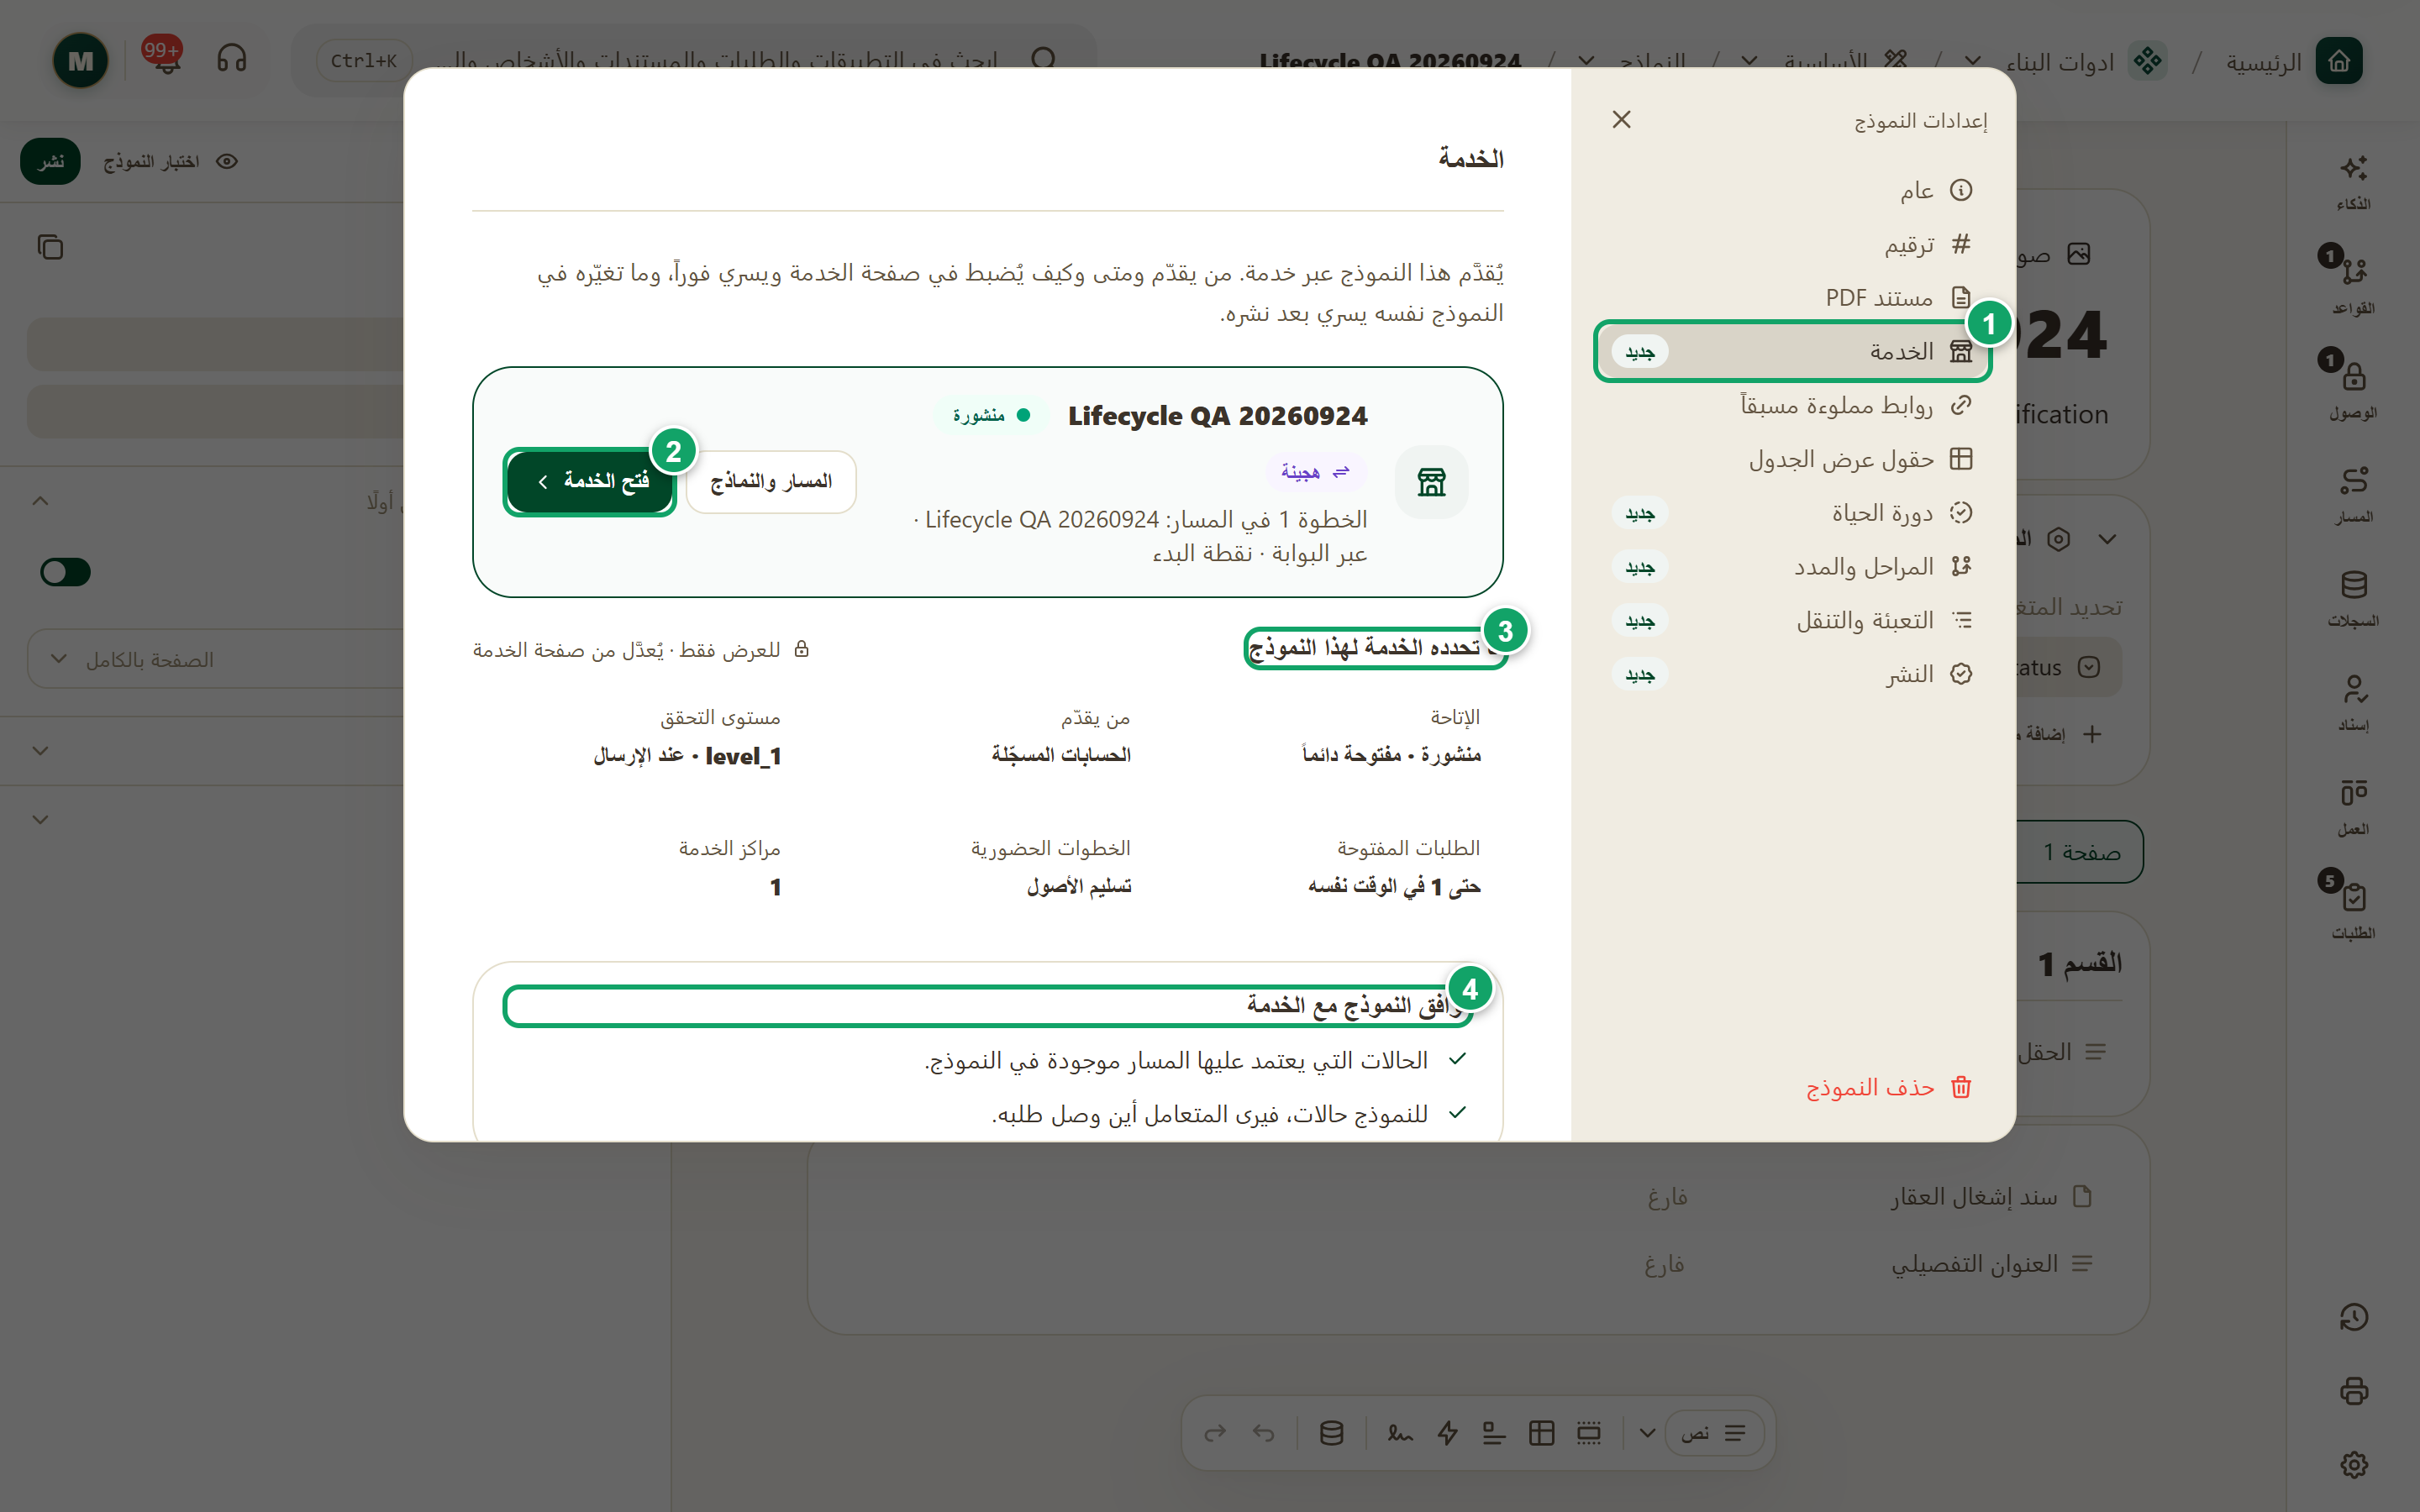
\includegraphics[width=0.95\linewidth,height=0.72\textheight,keepaspectratio]{figures/screens/ch06-services-form-settings-ar.png}
\caption{تبويب «الخدمة» في «إعدادات النموذج»}
\label{fig:builder-services-form-settings-screen}
\shotnote{تعرض الصورة تبويب «الخدمة» لنموذج البدء في خدمة هجينة بمؤسسة الاختبار، وفيه دور النموذج «الخطوة 1 في المسار» وإعدادات الخدمة التي تنطبق عليه. وتبيّن أن هذه الإعدادات «للعرض فقط»، فالتعديل يجري في صفحة الخدمة لا في منشئ النماذج. ① «الخدمة». ② «فتح الخدمة»: ينقلك إلى صفحة الخدمة لتعديلها. ③ «ما تحدده الخدمة لهذا النموذج»: الإتاحة ومن يقدّم والتحقق والحدود والمراكز. ④ «توافق النموذج مع الخدمة»: فحوص الحالات التي يعتمد عليها المسار.}
\end{figure}

\begin{table}[H]
\centering
\caption{ما يعرضه تبويب «الخدمة»}
\label{tab:builder-services-form-settings-parts}
\begin{tabularx}{\linewidth}{R{3.6cm} Y}
\rcHeaderRow
\thh{الجزء} & \thh{ما يعرضه أو يتيحه}\\
الخدمة ودور النموذج & اسم الخدمة ودور النموذج، مثل «الخطوة 1 في المسار» أو «نموذج خارج المسار، متاح في أي وقت»، مع رابطي «المسار والنماذج» و«فتح الخدمة».\\
ما تحدده الخدمة لهذا النموذج & «الإتاحة» و«من يقدّم» و«مستوى التحقق» و«الطلبات المفتوحة» و«الخطوات الحضورية» و«مراكز الخدمة»، وهي «للعرض فقط · يُعدَّل من صفحة الخدمة».\\
توافق النموذج مع الخدمة & يتحقق من وجود الحالات التي ينتظرها المسار في النموذج، ومن أن للنموذج حالات يرى بها المتعامل أين وصل طلبه.\\
إزالته من الخدمة & يجعل النموذج داخلياً ويخفيه من البوابة. ويُعطَّل لنموذج البدء في الخدمات التي تبدأ عبر البوابة حتى تعدّل المسار.\\
نموذج داخلي & للنموذج الذي لا ينتمي إلى خدمة، ومعه زر «إتاحته على البوابة».\\
معالجة الطلبات & مفتاح «مساحة المراجعة وتحديثات مقدمي الطلبات» لهذا النموذج، ومفتاح «إغلاق الطلب من المراسلات».\\
\end{tabularx}
\end{table}

\begin{figure}[H]
\centering
\begin{tikzpicture}[node distance=0.5cm]
\node[stepBox] (a) {\RL{فتح تبويب الخدمة}};
\node[stepBox,below=of a] (b) {\RL{قراءة دور النموذج}};
\node[stepBox,below=of b] (c) {\RL{مراجعة التوافق}};
\node[stepBox,below=of c] (d) {\RL{الإصلاح في النموذج أو الخدمة}};
\draw[flowsTo] (a) -- (b);
\draw[flowsTo] (b) -- (c);
\draw[flowsTo] (c) -- (d);
\end{tikzpicture}
\rclegend
\caption{فحص علاقة النموذج بخدمته}
\label{fig:builder-services-form-settings-flow}
\shotnote{يضع المخطط مراجعة التوافق قبل أي إصلاح، لأن التحذير يحدد مكان الحل: إما حالات النموذج في «دورة الحياة»، وإما خطوات الخدمة في «المسار والنماذج». ولا تُعدَّل إعدادات الخدمة من هذا التبويب، فهو للعرض فقط.}
\end{figure}

\subsection{خطوات العمل والتحقق}
\begin{enumerate}
\item افتح النموذج في منشئ النماذج، واضغط «الإعدادات» ثم «الخدمة».
\item اقرأ دور النموذج في الخدمة وما تحدده له.
\item راجع «توافق النموذج مع الخدمة»، وأصلح أي تحذير في «دورة الحياة» أو في «المسار والنماذج».
\item إذا لم ينتمِ النموذج إلى خدمة، فاضغط «إتاحته على البوابة» لتحويله إلى خدمة.
\end{enumerate}

\textbf{تحقق ومعالجة المشكلة:} يجب أن تظهر علامة صح بجانب كل فحص في «توافق النموذج مع الخدمة». فإذا ظهر «احفظ النموذج أولاً.»، فاحفظ النموذج الجديد ثم افتح التبويب من جديد. وإذا كان «إزالته من الخدمة» معطلاً، فغيّر نموذج البدء في «المسار والنماذج» أولاً.

\clearpage
\section{مكتب الاستقبال}
\label{sec:builder-feature-services-intake}

مكتب الاستقبال هو الصفحة التي يسجّل فيها موظف المركز طلب متعامل حضر بنفسه. فيختار الخدمة، ويبحث عن حساب المتعامل أو يسجّله دونه، ويؤشّر المستندات التي استلمها، ثم يعبّئ النموذج معه ويطبع إيصالاً برقم الطلب. وبذلك يدخل الطلب الحضوري في المتابعة نفسها التي تمر بها طلبات البوابة.

\textbf{المسار ومن يستخدمه:} «الخدمات» ← «مكتب الاستقبال». يستخدمه موظفو مراكز الخدمة يومياً، ويظهر فيه فقط ما فعّل «الاستقبال في المركز» من الخدمات.

\begin{rcnote}[مثال: شركة الأفق]
يحضر عميل إلى فرع حلب بلا حساب على البوابة، فيضغط عمر حداد «طلب حضوري جديد» ② ويختار «تسجيل مراجع بلا حساب»، ويكتب اسمه ورقم هاتفه. ثم يعبّئ النموذج معه ويضغط «تسجيل وطباعة الإيصال».
\end{rcnote}

\begin{figure}[H]
\centering
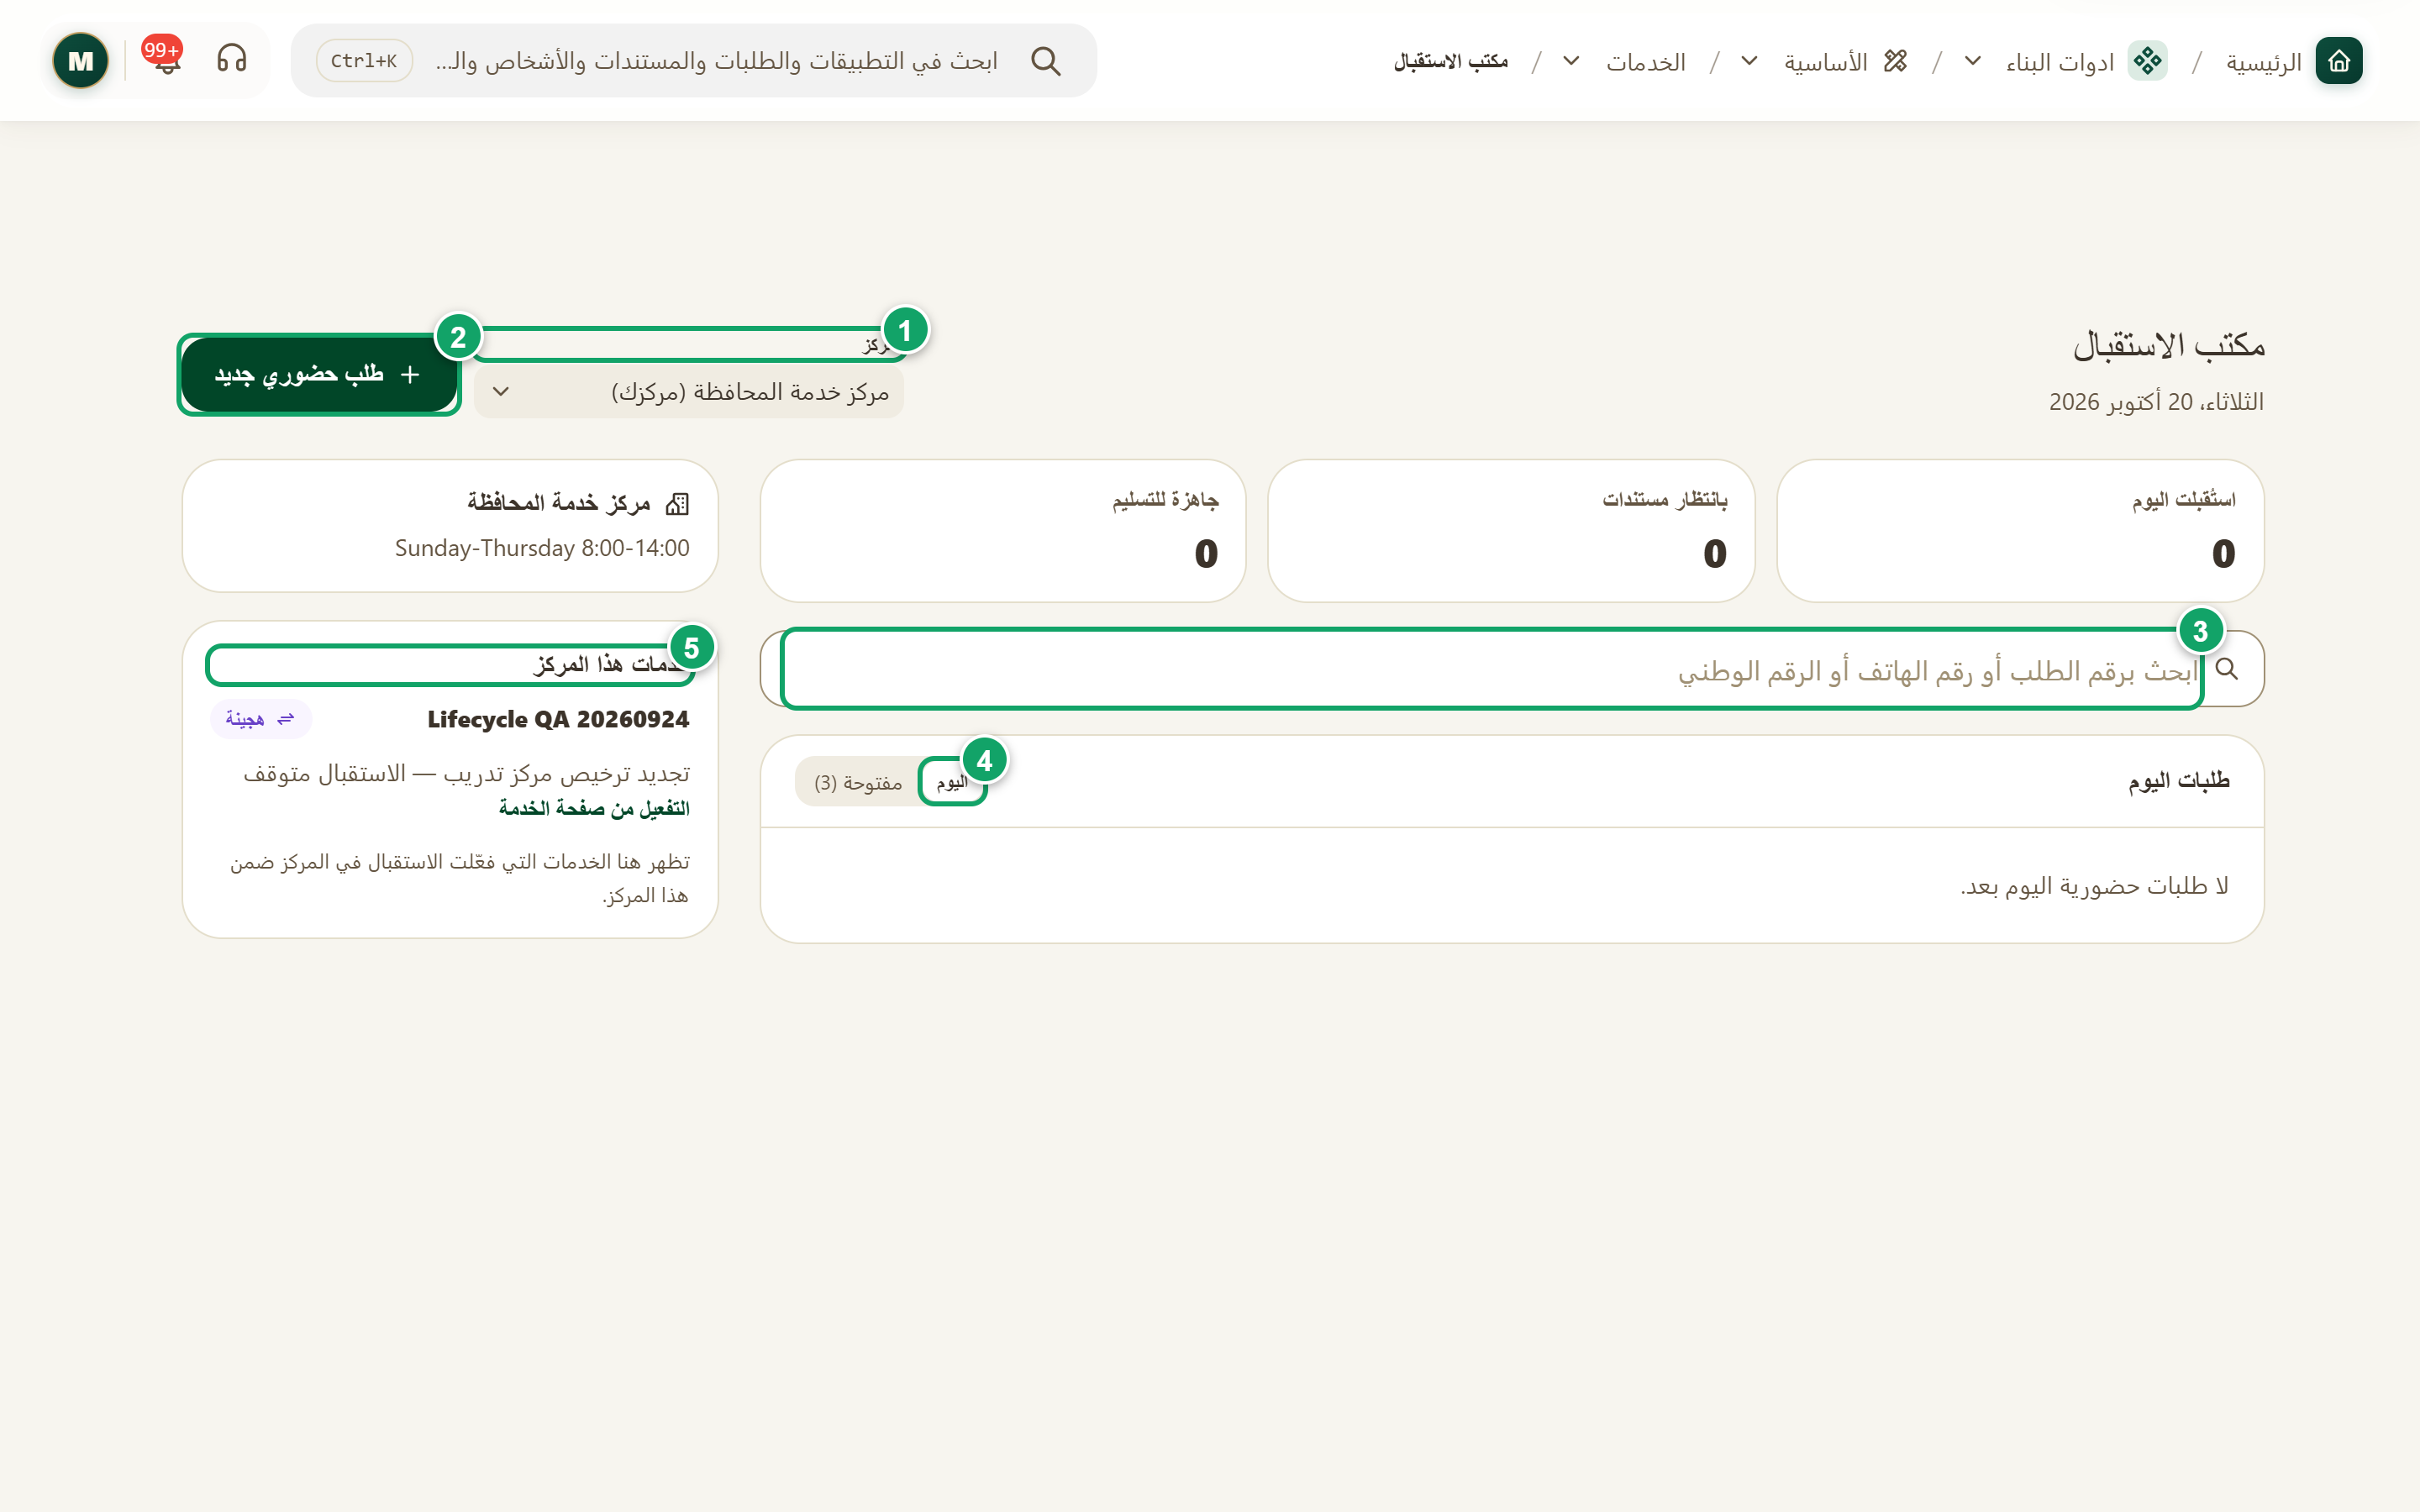
\includegraphics[width=0.95\linewidth,height=0.72\textheight,keepaspectratio]{figures/screens/ch06-services-intake-ar.png}
\caption{صفحة «مكتب الاستقبال»}
\label{fig:builder-services-intake-screen}
\shotnote{تعرض الصورة مكتب الاستقبال في مؤسسة الاختبار على «مركز خدمة المحافظة»، ولم يُسجَّل فيه طلب حضوري اليوم، لذلك تظهر المؤشرات أصفاراً. وتبيّن قائمة خدمات المركز أن خدمة واحدة تستقبل الطلبات، وأن أخرى متوقفة مع رابط لتفعيلها. ① «المركز». ② «طلب حضوري جديد»: يبدأ تسجيل طلب لمتعامل حاضر. ③ مربع البحث: يبحث برقم الطلب أو رقم الهاتف أو الرقم الوطني. ④ «اليوم»: يعرض طلبات اليوم، وبجانبه «مفتوحة». ⑤ «خدمات هذا المركز»: الخدمات التي فعّلت الاستقبال.}
\end{figure}

\begin{table}[H]
\centering
\caption{أجزاء مكتب الاستقبال}
\label{tab:builder-services-intake-desk}
\begin{tabularx}{\linewidth}{R{3.6cm} Y}
\rcHeaderRow
\thh{الجزء} & \thh{ما يعرضه أو يتيحه}\\
المركز & المركز الذي تعمل عليه، ويُعلَّم مركزك بعبارة «(مركزك)».\\
المؤشرات & «استُقبلت اليوم» أو «مفتوحة في هذا المركز»، و«بانتظار مستندات»، و«جاهزة للتسليم».\\
البحث والعرض & «ابحث برقم الطلب أو رقم الهاتف أو الرقم الوطني»، والتبديل بين «اليوم» و«مفتوحة».\\
جدول الطلبات & «رقم الطلب» و«المراجع» و«الخدمة» و«الحالة» و«استلمه» و«الوقت»، مع «عرض» أو «متابعة» و«طباعة الإيصال».\\
خدمات هذا المركز & الخدمات التي فعّلت الاستقبال، ورابط «التفعيل من صفحة الخدمة» لما توقف منها.\\
\end{tabularx}
\end{table}

\begin{table}[H]
\centering
\caption{صفحة «طلب حضوري جديد» والإيصال}
\label{tab:builder-services-intake-new}
\begin{tabularx}{\linewidth}{R{3.6cm} Y}
\rcHeaderRow
\thh{القسم} & \thh{ما تفعله فيه}\\
الخدمة والمراجع & تختار الخدمة، ثم تبحث بـ«رقم الهاتف أو البريد أو الرقم الوطني» عن حساب المراجع ليظهر الطلب في حسابه، أو تختار «تسجيل مراجع بلا حساب» وتكتب «الاسم الكامل» و«رقم الهاتف».\\
المستندات المستلمة & قائمة المستندات من دليل الخدمة. وإذا نقص مستند «مطلوب» يبقى الطلب «بانتظار مستندات».\\
ملخص & الحالة «عند التسجيل»، والرسم المستلم في المركز مع «رقم الإيصال»، ثم زر «إنشاء وتعبئة البيانات».\\
إيصال استلام طلب & يحمل «رقم الطلب» والمستندات المستلمة وغير المستلمة، وطريقة «تتبّع طلبك» برقم الطلب ورقم الهاتف، ودوام المركز.\\
\end{tabularx}
\end{table}

\begin{figure}[H]
\centering
\begin{tikzpicture}[node distance=0.5cm]
\node[stepBox] (a) {\RL{طلب حضوري جديد}};
\node[stepBox,below=of a] (b) {\RL{الخدمة والمراجع}};
\node[stepBox,below=of b] (c) {\RL{المستندات المستلمة}};
\node[stepBox,below=of c] (d) {\RL{إنشاء وتعبئة البيانات}};
\node[stepBox,below=of d] (e) {\RL{تسجيل وطباعة الإيصال}};
\draw[flowsTo] (a) -- (b);
\draw[flowsTo] (b) -- (c);
\draw[flowsTo] (c) -- (d);
\draw[flowsTo] (d) -- (e);
\end{tikzpicture}
\rclegend
\caption{تسجيل طلب حضوري}
\label{fig:builder-services-intake-flow}
\shotnote{يُنشأ الطلب أولاً ثم يُعبَّأ نموذجه، ولا يأخذ رقمه إلا عند الخطوة الأخيرة، لذلك يظهر في الجدول بعبارة «غير مسجّل» حتى تُكمله. وإذا نقص مستند مطلوب، يبقى الطلب بانتظاره حتى تضغط «استُلمت المستندات — إرسال الطلب».}
\end{figure}

\subsection{خطوات العمل والتحقق}
\begin{enumerate}
\item افتح «الخدمات» واضغط «مكتب الاستقبال»، وتأكد من «المركز».
\item اضغط «طلب حضوري جديد»، واختر الخدمة، ثم ابحث عن المراجع أو سجّله بلا حساب.
\item أشّر المستندات المستلمة، وسجّل «رقم الإيصال» إن استلمت الرسم، ثم اضغط «إنشاء وتعبئة البيانات».
\item عبّئ النموذج مع المراجع، ثم اضغط «تسجيل وطباعة الإيصال».
\item اضغط «طباعة» في صفحة الإيصال وسلّمه للمراجع.
\end{enumerate}

\textbf{تحقق ومعالجة المشكلة:} يظهر الطلب في الجدول برقمه واسم من استلمه. فإذا ظهر «أكمل الإجابات المطلوبة في النموذج قبل تسجيل الطلب.»، فأكمل الحقول الناقصة. وإذا ظهر «لا تستقبل أي خدمة طلبات حضورية في هذا المركز بعد»، ففعّل «الاستقبال في المركز» في تبويب «التقديم والأهلية» للخدمة.

\clearpage
\section{أداء الخدمات}
\label{sec:builder-feature-services-performance}

تجيب صفحة «أداء الخدمات» عن أسئلة الإدارة: كم طلباً وصل، وكم استغرق إنجازه، وأين يتأخر، وما رأي المتعاملين. وتُحتسب فيها الطلبات المرسلة من البوابة، ولا يدخل وقت انتظار المتعامل في مدد المراحل والإنجاز. لذلك تعطيك صورة عادلة عن أداء فريقك، وتدلك على المرحلة التي تحتاج إلى دعم.

\textbf{المسار ومن يستخدمه:} «الخدمات» ← «أداء الخدمات»، أو رابط «الأداء الكامل» في «نظرة عامة». يستخدمها مديرو الخدمات في مراجعتهم الدورية.

\begin{rcnote}[مثال: شركة الأفق]
تختار سارة الخطيب «آخر 30 يوم» ① وخدمة «طلب زيارة فرع»، فترى في «طلبات تجاوزت المدة» ③ طلباً متأخراً في مرحلة المراجعة. فتضغط «تصعيد» بجانبه، ثم تصدّر المؤشرات بزر «تصدير» ④ لاجتماعها الشهري.
\end{rcnote}

\begin{figure}[H]
\centering
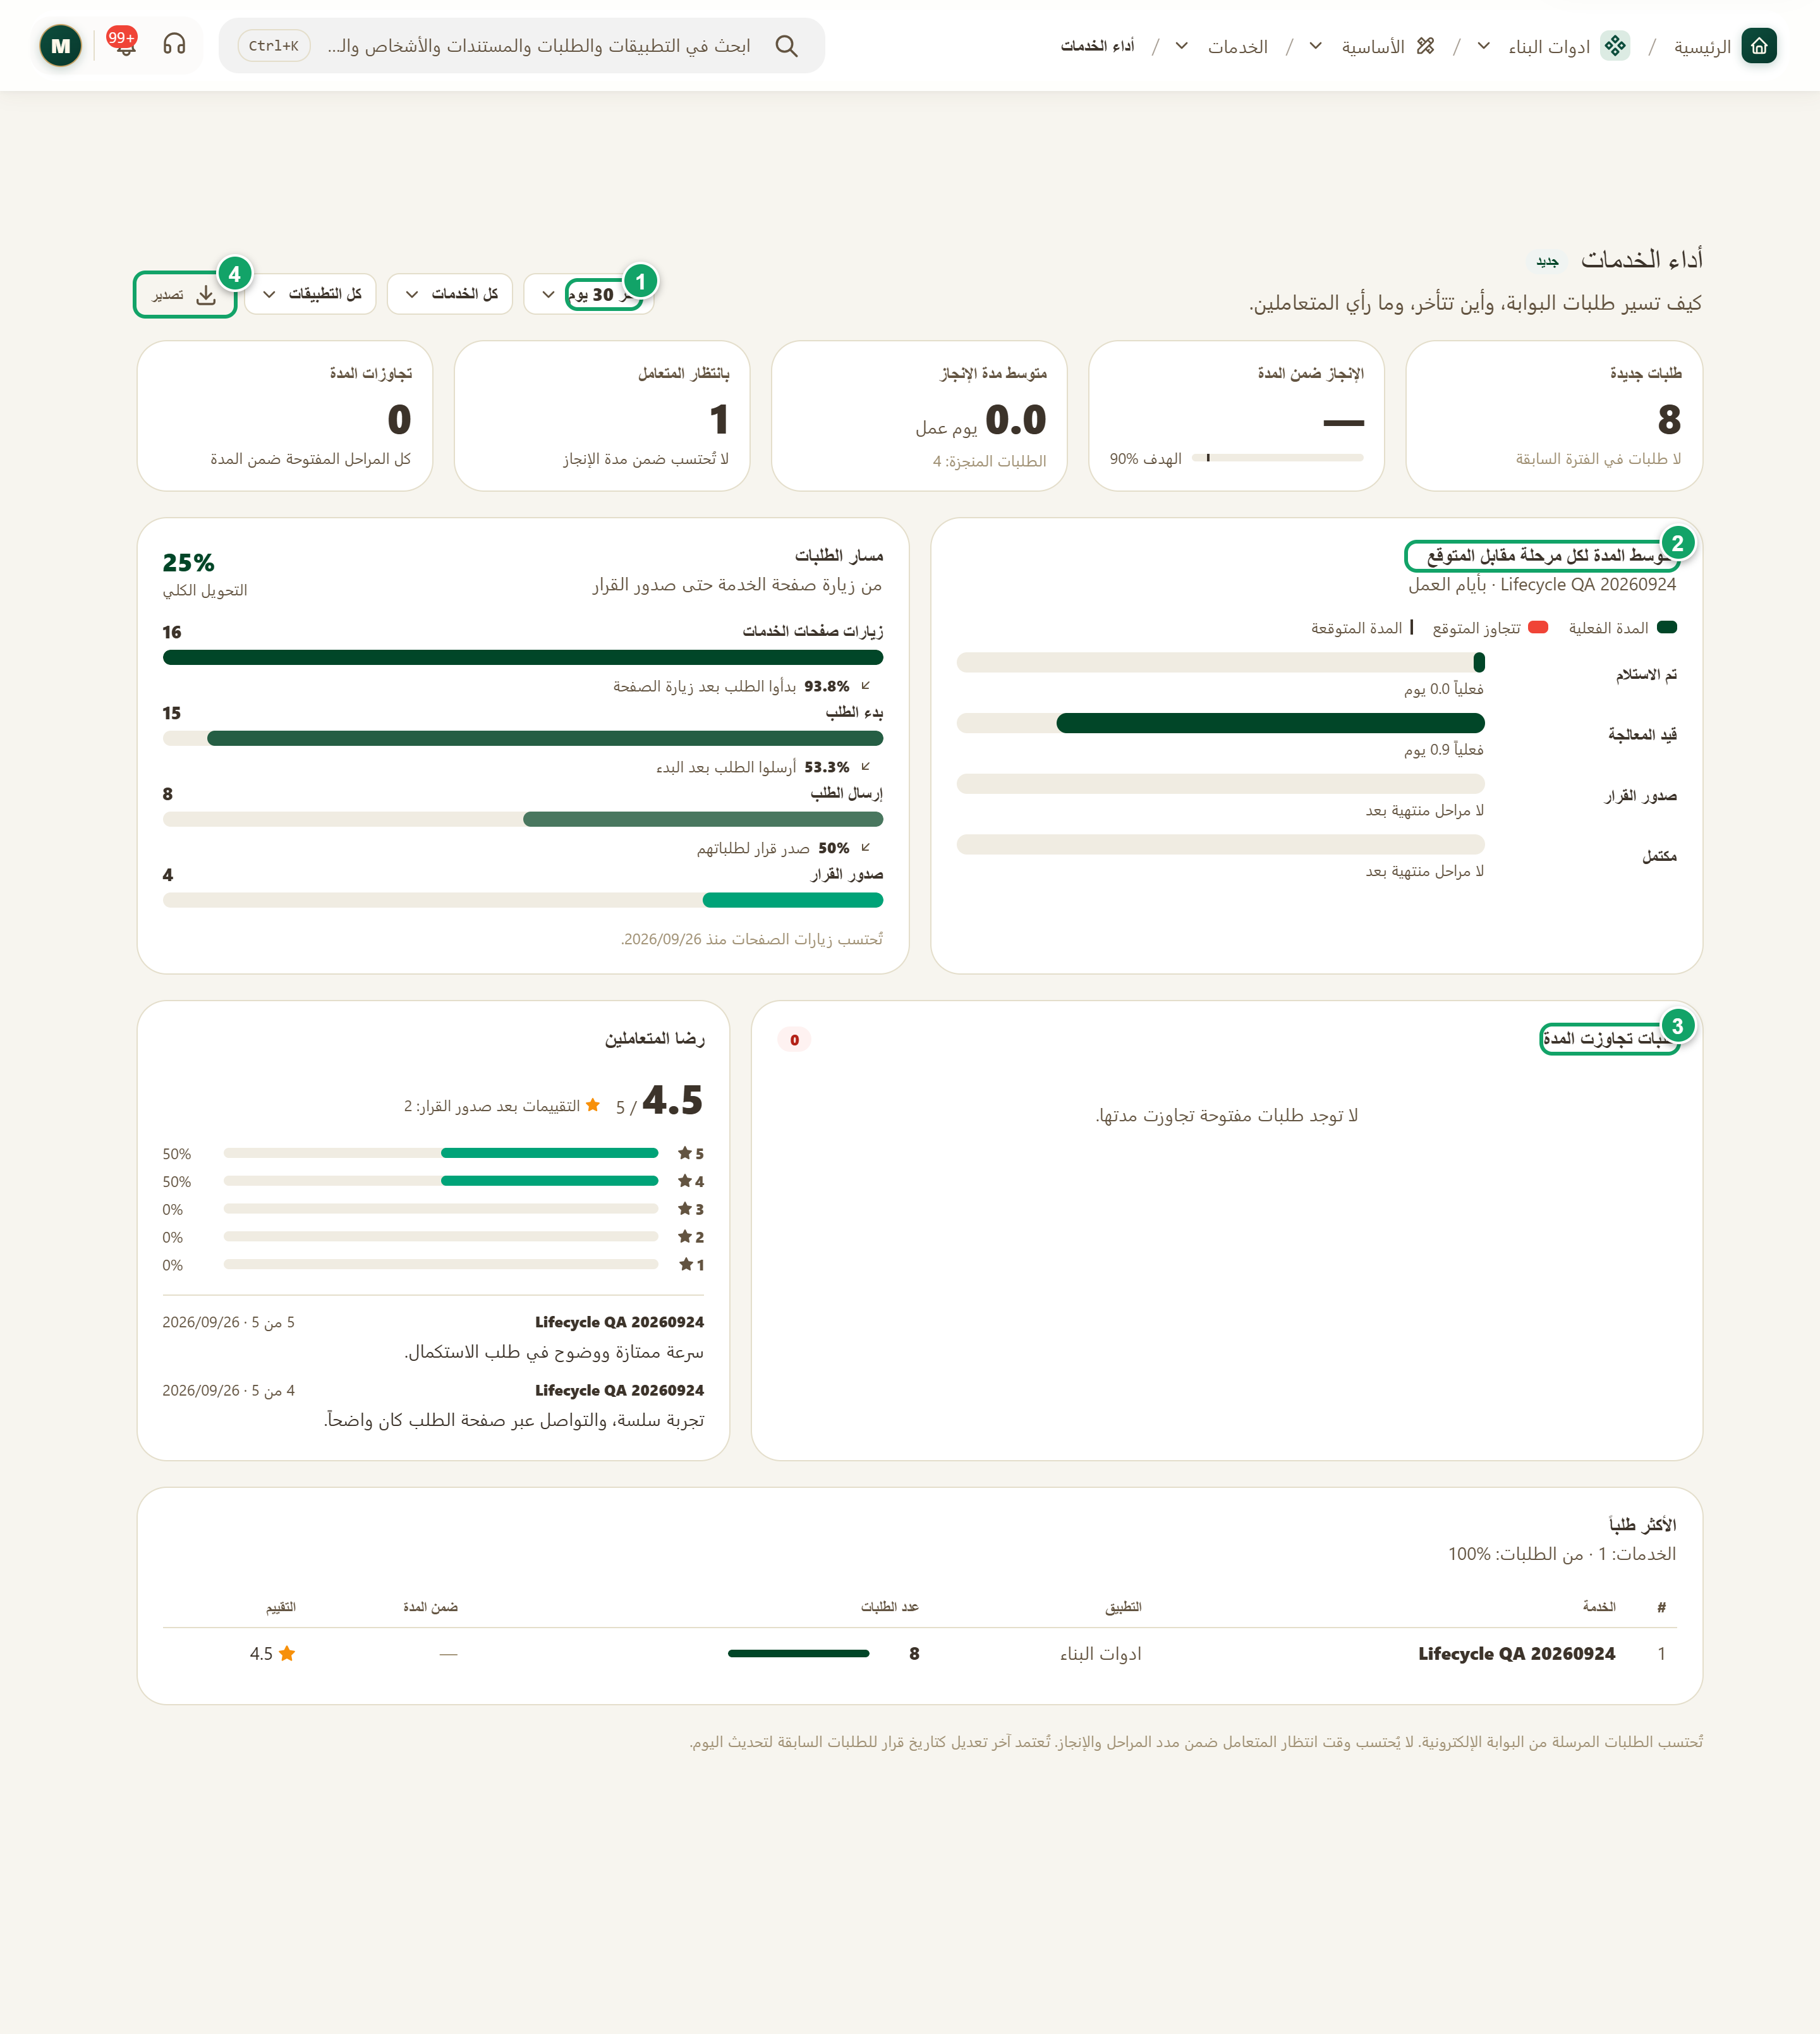
\includegraphics[width=0.95\linewidth,height=0.72\textheight,keepaspectratio]{figures/screens/ch06-services-performance-ar.png}
\caption{صفحة «أداء الخدمات»}
\label{fig:builder-services-performance-screen}
\shotnote{تعرض الصورة أداء خدمات مؤسسة الاختبار خلال آخر 30 يوماً، ولا يوجد فيها طلب تجاوز مدته، لذلك يظهر جدول التجاوزات فارغاً. وتبيّن أن الصفحة تنتقل من المؤشرات العامة إلى المراحل ثم إلى الطلبات الفردية. ① «آخر 30 يوم»: الفترة، وبجانبها تصفية الخدمة والتطبيق. ② «متوسط المدة لكل مرحلة مقابل المتوقع». ③ «طلبات تجاوزت المدة»: الطلبات المتأخرة مع زر «تصعيد». ④ «تصدير».}
\end{figure}

\begin{table}[H]
\centering
\caption{مؤشرات «أداء الخدمات»}
\label{tab:builder-services-performance-kpis}
\begin{tabularx}{\linewidth}{R{3.6cm} Y}
\rcHeaderRow
\thh{المؤشر} & \thh{ما يقيسه}\\
طلبات جديدة & عدد الطلبات في الفترة، مقارنة بالفترة السابقة.\\
الإنجاز ضمن المدة & نسبة المراحل التي انتهت في وقتها، مقابل هدف يظهر تحت المؤشر.\\
متوسط مدة الإنجاز & متوسط أيام العمل حتى صدور القرار، وعدد الطلبات المنجزة.\\
بانتظار المتعامل & الطلبات التي تنتظر إجراءً من مقدّمها، ولا تُحتسب ضمن مدة الإنجاز.\\
تجاوزات المدة & عدد الطلبات المفتوحة التي تجاوزت مدة مرحلتها، والمرحلة الأكثر تأخراً.\\
\end{tabularx}
\end{table}

\begin{table}[H]
\centering
\caption{بطاقات التحليل}
\label{tab:builder-services-performance-cards}
\begin{tabularx}{\linewidth}{R{3.6cm} Y}
\rcHeaderRow
\thh{البطاقة} & \thh{ما تعرضه}\\
متوسط المدة لكل مرحلة مقابل المتوقع & المدة الفعلية لكل مرحلة بأيام العمل مقارنة بالمدة المتوقعة المحددة في «المراحل والمدد» في النموذج، للخدمة المختارة أو الأكثر طلباً.\\
مسار الطلبات & من «زيارات صفحات الخدمات» إلى «بدء الطلب» ثم «إرسال الطلب» ثم «صدور القرار»، مع «التحويل الكلي».\\
طلبات تجاوزت المدة & «رقم الطلب» و«الخدمة» و«المرحلة» و«المسؤول» و«التجاوز»، مع زر «تصعيد».\\
رضا المتعاملين والأكثر طلباً & متوسط التقييمات بعد صدور القرار، وجدول الخدمات الأكثر طلباً مع نسبتها من الطلبات وتقييمها.\\
\end{tabularx}
\end{table}

\begin{figure}[H]
\centering
\begin{tikzpicture}[node distance=0.5cm]
\node[stepBox] (a) {\RL{الفترة والخدمة}};
\node[stepBox,below=of a] (b) {\RL{قراءة المؤشرات}};
\node[stepBox,below=of b] (c) {\RL{تحديد المرحلة المتأخرة}};
\node[stepBox,below=of c] (d) {\RL{تصعيد الطلبات المتأخرة}};
\node[stepBox,below=of d] (e) {\RL{التصدير للمراجعة}};
\draw[flowsTo] (a) -- (b);
\draw[flowsTo] (b) -- (c);
\draw[flowsTo] (c) -- (d);
\draw[flowsTo] (d) -- (e);
\end{tikzpicture}
\rclegend
\caption{مراجعة دورية لأداء الخدمات}
\label{fig:builder-services-performance-flow}
\shotnote{ينتقل المخطط من الصورة العامة إلى الطلب الواحد: المؤشرات تبيّن وجود تأخر، وبطاقة المراحل تحدد مكانه، وجدول التجاوزات يسمح بتصعيد كل طلب على حدة. ويأتي التصدير أخيراً ليحفظ نتيجة المراجعة في ملف.}
\end{figure}

\subsection{خطوات العمل والتحقق}
\begin{enumerate}
\item افتح «الخدمات» واضغط «أداء الخدمات».
\item اختر «الفترة»: 7 أو 30 أو 90 يوماً، ثم اختر الخدمة أو التطبيق إن أردت التضييق.
\item قارن المدة الفعلية بالمتوقعة في بطاقة المراحل، وحدد المرحلة التي تتجاوز المتوقع.
\item اضغط «تصعيد» بجانب كل طلب متأخر يحتاج إلى تدخل.
\item اضغط «تصدير» لتحفظ المؤشرات في ملف.
\end{enumerate}

\textbf{تحقق ومعالجة المشكلة:} بعد التصعيد يتحول الزر إلى «تم التصعيد» ولا يمكن الضغط عليه مرة أخرى. وإذا ظهر «لا توجد مراحل للمقارنة بعد.»، فحدد مراحل النموذج ومددها في «المراحل والمدد». وإذا ظهر «تعذّر تحميل أداء الخدمات.»، فأعد تحميل الصفحة.


\chapter{الإجراءات الداخلية}
\label{ch:builder-internal-sops}

\section{ماذا ستبني في هذا الفصل؟}
\label{sec:builder-internal-sops-intro}

الإجراء الداخلي مسار عمل من خطوات متتابعة يبدأ عند حدث تحدده، مثل إنشاء سجل أو إرسال نموذج. وقد تطلب خطواته موافقة، أو تُنشئ مهمة، أو ترسل إشعاراً، فلا يعتمد إنجاز العمل على أن يتذكر أحد الخطوة التالية. ويشرح هذا الفصل الأداة كاملة: الصفحة الرئيسية، والمحرر، والمشغّلات وأنواع الخطوات، وإعداد كل خطوة ومعالجة أخطائها، ثم الاختبار والنشر ومتابعة عمليات التشغيل والرد على الموافقات.

وتُحفظ تعديلاتك في مسودة لا تعمل حتى تنشرها، لذلك يمر كل إجراء بالدورة نفسها: تبنيه، ثم تختبره، ثم تنشره، ثم تتابع تشغيله.

\begin{rcnote}[مثال: شركة الأفق]
عند إنشاء طلب زيارة جديد يطلب إجراء داخلي موافقة سارة الخطيب، وبعد موافقتها يُنشئ مهمة تحضير الزيارة لعمر حداد.
\end{rcnote}

\begin{figure}[H]
\centering
\begin{tikzpicture}[node distance=0.5cm]
\node[stepBox] (a) {\RL{المشغّل: ما الذي يبدأه؟}};
\node[stepBox,below=of a] (b) {\RL{الخطوات وإعدادها}};
\node[stepBox,below=of b] (c) {\RL{اختبار: محاكاة آمنة}};
\node[stepBox,below=of c] (d) {\RL{مراجعة ونشر}};
\node[stepBox,below=of d] (e) {\RL{متابعة عمليات التشغيل}};
\draw[flowsTo] (a) -- (b);
\draw[flowsTo] (b) -- (c);
\draw[flowsTo] (c) -- (d);
\draw[flowsTo] (d) -- (e);
\end{tikzpicture}
\rclegend
\caption{دورة حياة الإجراء الداخلي}
\label{fig:builder-internal-sops-overview}
\shotnote{يرتب المخطط صفحات هذا الفصل بحسب دورة الإجراء. فالاختبار يسبق النشر لأن المحاكاة لا تُحدث أي أثر، والمتابعة تأتي بعد النشر لأن الإجراء لا يبدأ أي تشغيل قبله.}
\end{figure}

\section{صفحات هذا الفصل}
\label{sec:builder-internal-sops-pages}

تبدأ من صفحة «الإجراءات الداخلية» في قسم «الأساسية» من أدوات البناء، أما بقية الصفحات فتشرح أجزاء المحرر وتبويبات الصفحة نفسها. واتبع ترتيبها في المرة الأولى، ثم عُد إلى أي صفحة عند الحاجة.

\begin{table}[H]
\centering
\caption{تشغيل العمل بالإجراءات الداخلية}
\label{tab:builder-pages-internal-sops}
\rcZebra
\begin{tabularx}{\linewidth}{R{4.2cm} Y}
\rcHeaderRow
\thh{الصفحة وقسمها} & \thh{ماذا تقدم هذه الصفحة؟}\\
الإجراءات الداخلية — الأساسية & تعرض الإجراءات في مجلدات مع حالتها وصحة تشغيلها، ومنها تنشئ إجراءً جديداً.\\
محرر الإجراء وأوضاعه — المحرر & رأس المحرر وأوضاع «بناء» و«اختبار» و«عمليات التشغيل»، وقائمة الخطوات واللوحة وأدواتها.\\
المشغّلات: ما الذي يبدأ الإجراء؟ — المحرر & مجموعات المشغّلات، ومشغّلات السجلات والنماذج والمهام والموافقات، وتغيير المشغّل.\\
خطوات التحكم في المسار — المحرر & التفرّع الشرطي والتكرار والتأخير والانتظار والإنهاء واستدعاء إجراء آخر.\\
خطوات السجلات والنماذج — المحرر & البحث عن السجلات وإنشاؤها وتحديثها، وطلب تعبئة النماذج.\\
خطوات المهام والموافقات والإشعارات والمستندات — المحرر & إنشاء المهام وطلب الموافقة والتوقيع وإرسال الإشعارات وإنشاء المستندات.\\
إعداد الخطوة: المدخلات والبيانات والتعبيرات — المحرر & لوحة إعداد الخطوة، وإدراج البيانات من الخطوات السابقة، والتعبيرات والاسم المرجعي.\\
معالجة الأخطاء وتخطي الخطوات — المحرر & الإيقاف أو مسار الفشل عند الخطأ، وإعادة المحاولة، وتخطي الخطوة.\\
الاتصالات والمتغيرات — الإجراءات الداخلية & حسابات الخدمات الخارجية، والقيم المشفرة التي تستخدمها التعبيرات.\\
اختبار الإجراء — المحرر & المحاكاة الآمنة والتشغيل الفعلي واختبار خطوة واحدة.\\
عمليات التشغيل وسجلها — المحرر والإجراءات الداخلية & حالات التشغيل، وقراءة النتائج على اللوحة، وإعادة التشغيل أو إلغاؤه.\\
الرد على طلبات الموافقة — طلبات بانتظارك & كيف يرد المعتمد، وما يحدث بعد كل رد.\\
المراجعة والنشر وسجل الإصدارات — المحرر & ما يجب إصلاحه والتغييرات قبل النشر، والإصدارات المقفلة والإيقاف المؤقت.\\
\end{tabularx}
\end{table}

\clearpage
\section{الإجراءات الداخلية}
\label{sec:builder-feature-internal-sops}

صفحة «الإجراءات الداخلية» هي نقطة البداية لكل إجراء تبنيه. فهي تعرض الإجراءات الموجودة في مجلدات، وتبيّن حالة كل إجراء ونتائج عمليات تشغيله الأخيرة، ومنها تنشئ إجراءً جديداً أو تفتح إجراءً قائماً لتعديله. وتساعدك مؤشرات الصحة فيها على ملاحظة الإجراء الذي بدأ يفشل قبل أن يشتكي أحد.

\textbf{المسار ومن يستخدمه:} «ادوات البناء» ← «الأساسية» ← «الإجراءات الداخلية». يستخدمها من يصمم مسارات العمل في المؤسسة ويتابع تشغيلها.

\begin{rcnote}[مثال: شركة الأفق]
يبني مسؤول النظام إجراء «اعتماد طلب الزيارة» يبدأ «عند إرسال نموذج» طلب الزيارة، فيرسل «طلب موافقة» إلى سارة الخطيب، ثم يُنشئ لعمر حداد مهمة تجهيز الزيارة إذا وافقت. ويبدأ الإجراء من ② ويتابع عمليات تشغيله من ④.
\end{rcnote}

\begin{figure}[H]
\centering
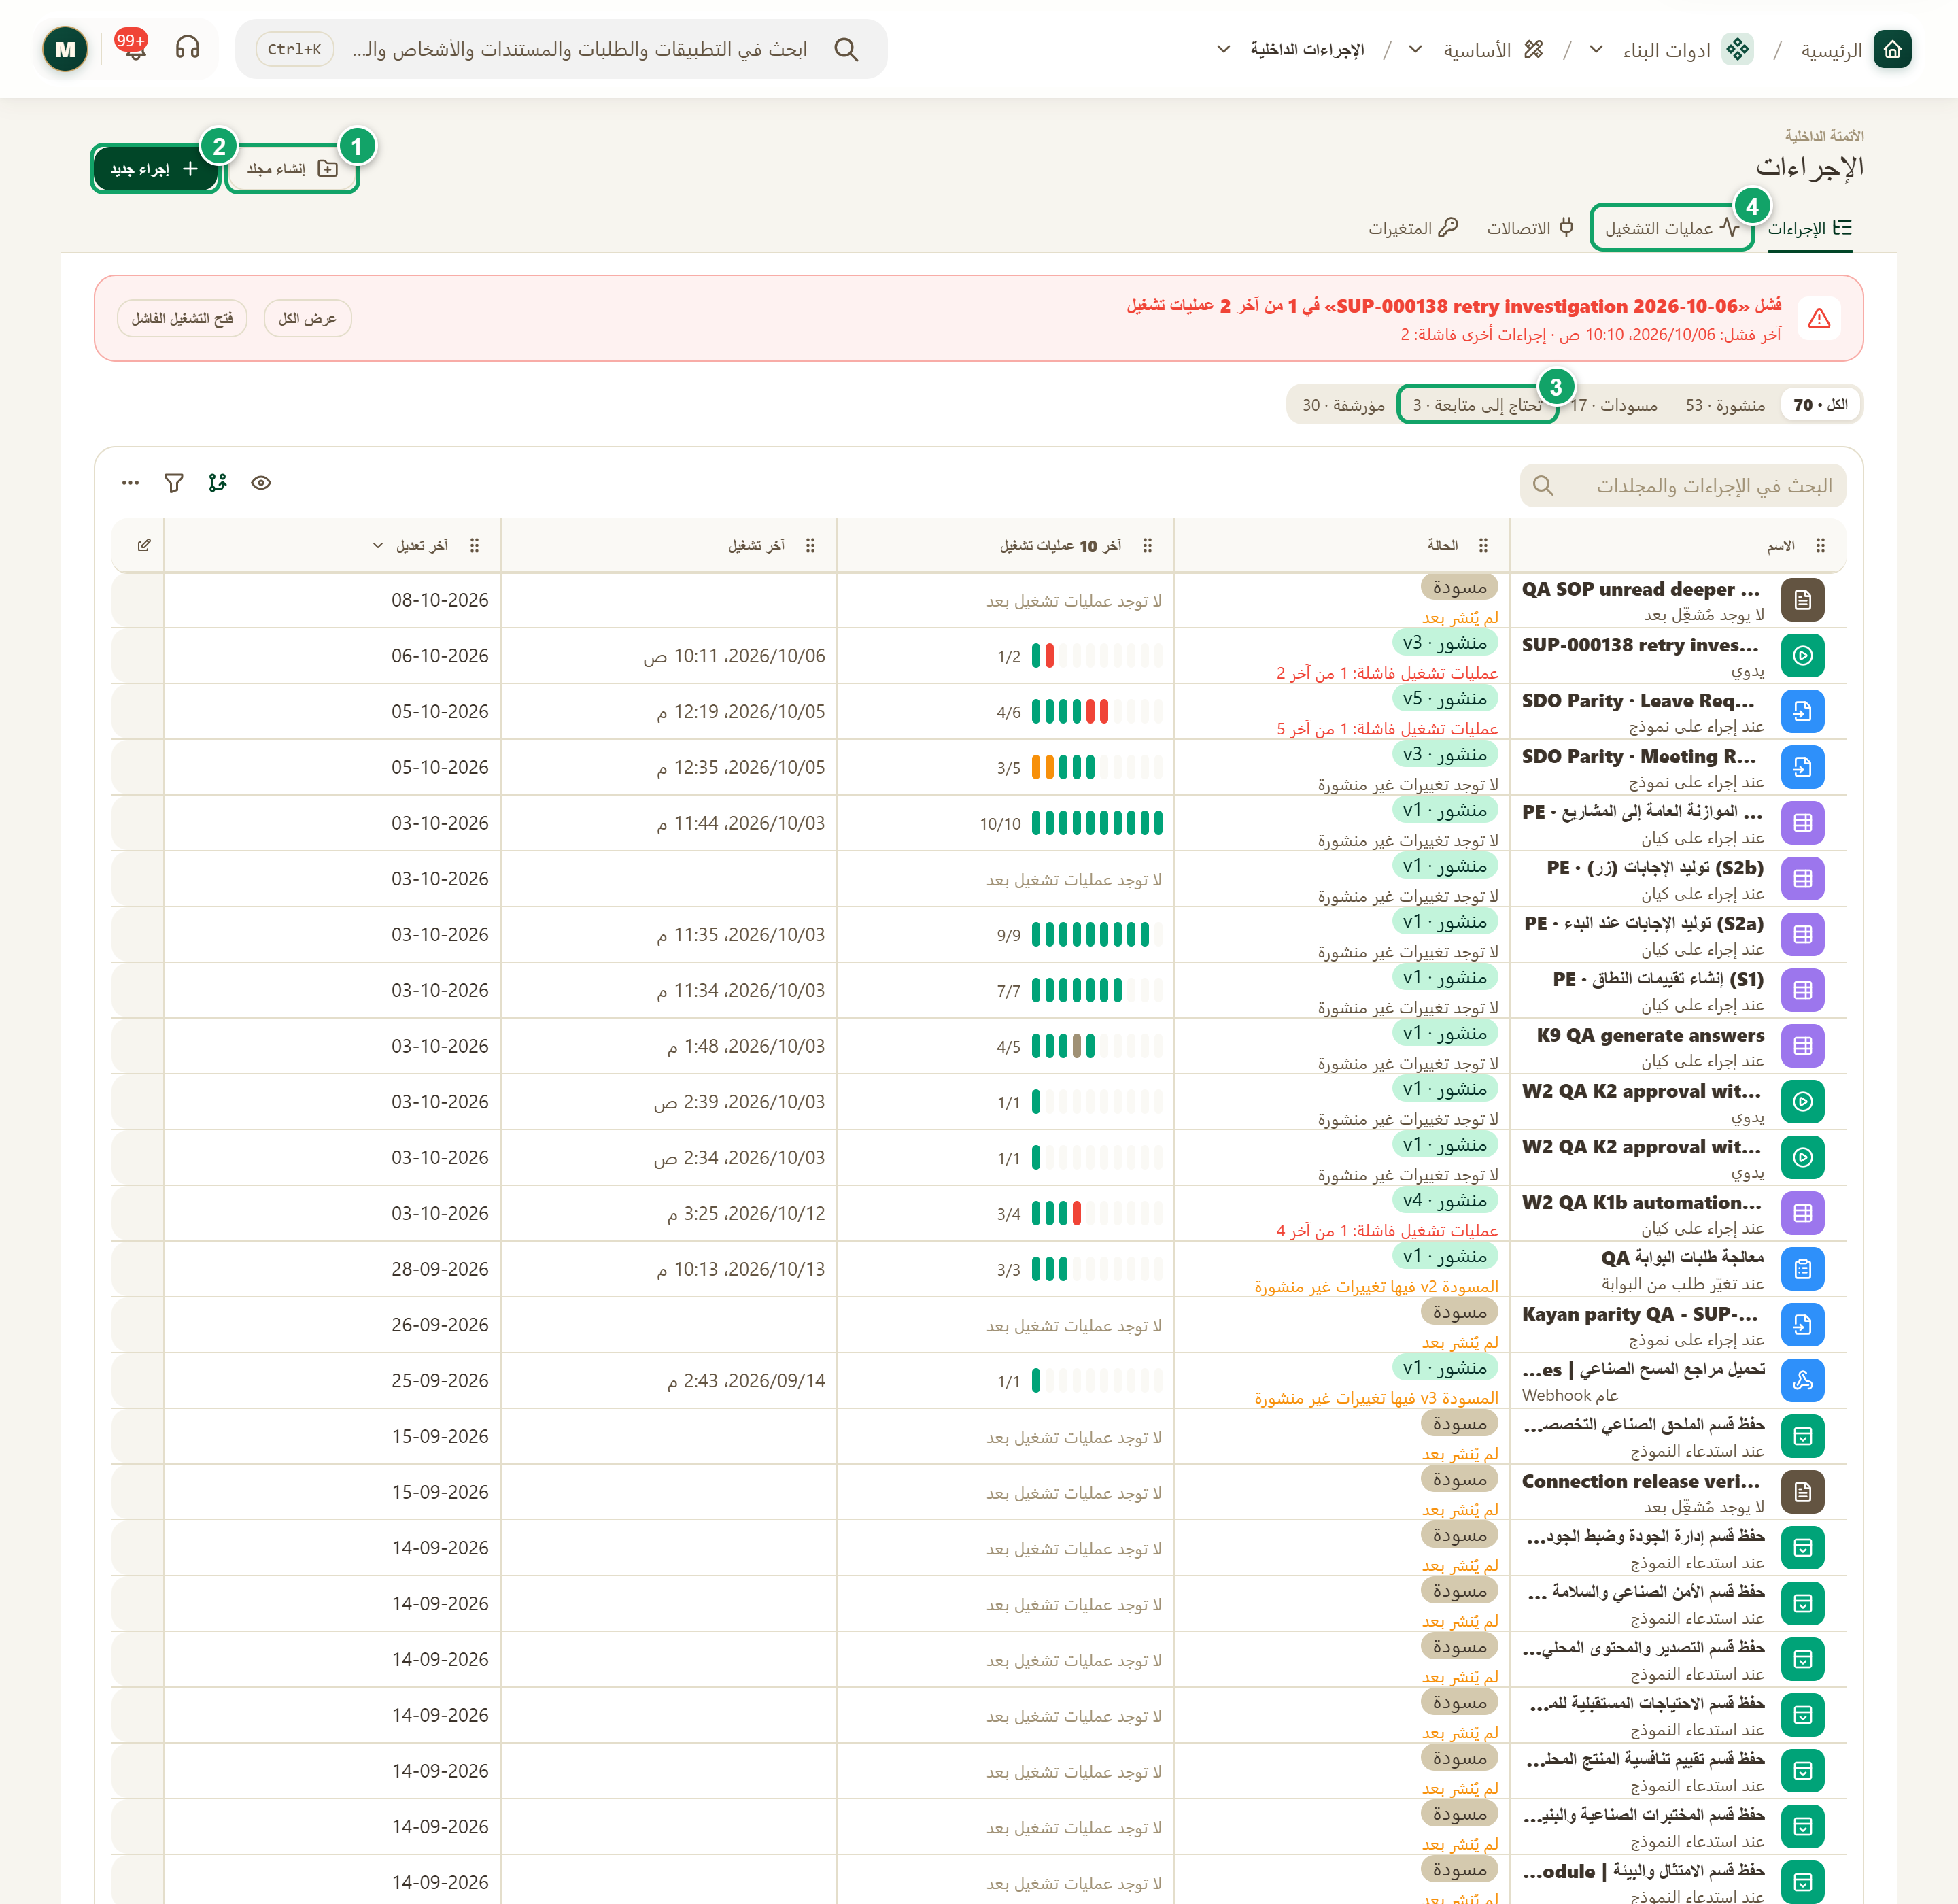
\includegraphics[width=0.95\linewidth,height=0.72\textheight,keepaspectratio]{figures/screens/ch06-internal-sops-ar.png}
\caption{صفحة «الإجراءات الداخلية»}
\label{fig:builder-internal-sops-screen}
\shotnote{تعرض الصورة أعلى قائمة الإجراءات في مؤسسة الاختبار، وفيها عشرات الإجراءات الاختبارية بحالاتها ونتائج آخر عمليات تشغيلها، ويسبقها تنبيه بإجراء فشل مؤخراً. وتبيّن الصورة أن الصفحة نفسها تنبهك إلى الإجراء المتعثر قبل أن تبحث عنه. ① «إنشاء مجلد»: ينظّم الإجراءات في مجلدات. ② «إجراء جديد»: يبدأ إجراءً ويطلب ما الذي يبدأه. ③ «تحتاج إلى متابعة»: يعرض الإجراءات المنشورة التي فشلت عمليات تشغيلها مؤخراً. ④ «عمليات التشغيل»: آخر عمليات التشغيل لكل الإجراءات.}
\end{figure}

\begin{table}[H]
\centering
\caption{ما الذي تجده في الصفحة؟}
\label{tab:builder-internal-sops-data}
\begin{tabularx}{\linewidth}{R{3.6cm} Y}
\rcHeaderRow
\thh{الجزء} & \thh{ما يقدمه}\\
التبويبات & «الإجراءات» وهو التبويب الافتراضي، و«عمليات التشغيل» لكل الإجراءات، و«الاتصالات»، و«المتغيرات».\\
التصفية & «الكل» و«منشورة» و«مسودات» و«تحتاج إلى متابعة» و«مؤرشفة»، مع عدد الإجراءات بجانب كل خيار. ويظهر «متوقفة مؤقتًا» عند وجود إجراء موقوف.\\
أعمدة القائمة & اسم الإجراء ومشغّله، و«الحالة» مثل «منشور · \en{v2}» أو «مسودة»، و«آخر 10 عمليات تشغيل» بنسبة الناجح منها، و«آخر تشغيل»، و«آخر تعديل».\\
تنبيه الفشل & يظهر أعلى القائمة عندما يفشل إجراء منشور في واحدة على الأقل من آخر خمس عمليات تشغيل، ومعه «فتح التشغيل الفاشل» و«عرض الكل».\\
المجلدات & «إنشاء مجلد» في رأس الصفحة. ومن قائمة المجلد تعيد تسميته، وتنشئ داخله إجراءً أو مجلداً فرعياً، وتنقله، وتحذفه.\\
قائمة الإجراء & «نقل إلى» مجلد آخر، و«إيقاف الإجراء مؤقتًا» أو «استئناف» للإجراء المنشور، وأمر الأرشفة الذي يظهر باسم «الأرشيف»، و«استعادة» للإجراء المؤرشف.\\
\end{tabularx}
\end{table}

\subsection{إنشاء إجراء جديد}

يفتح زر «إجراء جديد» لوحة جانبية تطلب أمرين فقط: الاسم، والإجابة عن «ما الذي يبدأه؟». وتعرض اللوحة أكثر المشغّلات استخداماً، وهي «عند إرسال نموذج» و«إنشاء سجل جديد» و«جدولة» و«عند انتهاء موافقة» و«Webhook عام» و«يدوي»، أما بقية المشغّلات فتجدها خلف «مزيد من المُشغِّلات». ويمكنك تغيير الاسم والمشغّل لاحقاً من المحرر.

\begin{rcwarn}[حذف مجلد فيه إجراءات]
إذا حذفت مجلداً يحتوي على إجراءات أو مجلدات فرعية، يطلب منك النظام أن تختار مصير المحتوى: إما نقله إلى جذر القائمة، وإما أرشفته مع حذف المجلد. أما المجلد الفارغ فيُحذف مباشرة.
\end{rcwarn}

\begin{figure}[H]
\centering
\begin{tikzpicture}[node distance=0.5cm]
\node[stepBox] (a) {\RL{إجراء جديد}};
\node[stepBox,below=of a] (b) {\RL{كتابة الاسم}};
\node[stepBox,below=of b] (c) {\RL{اختيار ما الذي يبدأه}};
\node[stepBox,below=of c] (d) {\RL{إنشاء وفتح}};
\node[stepBox,below=of d] (e) {\RL{المحرر: بناء الخطوات}};
\draw[flowsTo] (a) -- (b);
\draw[flowsTo] (b) -- (c);
\draw[flowsTo] (c) -- (d);
\draw[flowsTo] (d) -- (e);
\end{tikzpicture}
\rclegend
\caption{إنشاء إجراء من الصفحة الرئيسية}
\label{fig:builder-internal-sops-flow}
\shotnote{يبيّن المخطط أن الإجراء لا يُنشأ دون مشغّل، لأن الزر «إنشاء وفتح» يبقى معطلاً حتى تختار ما الذي يبدأه. وبعد الإنشاء تنتقل مباشرة إلى المحرر، فيكون الإجراء مسودة لا تعمل حتى تنشرها.}
\end{figure}

\subsection{خطوات العمل والتحقق}
\begin{enumerate}
\item افتح «الإجراءات الداخلية»، وإذا أردت ترتيب الإجراءات فاضغط «إنشاء مجلد» واكتب «اسم المجلد».
\item اضغط «إجراء جديد»، أو اختر من قائمة المجلد أمر إنشاء الإجراء داخله.
\item اكتب الاسم، واختر مشغّلاً من الخيارات الشائعة أو من «مزيد من المُشغِّلات»، ثم اضغط «إنشاء وفتح».
\item عُد إلى القائمة لاحقاً، واختر «تحتاج إلى متابعة» لترى الإجراءات المنشورة التي فشلت عمليات تشغيلها مؤخراً.
\end{enumerate}

\textbf{تحقق ومعالجة المشكلة:} يجب أن يفتح المحرر على الإجراء الجديد، وأن يظهر في القائمة بحالة «مسودة» مع ملاحظة «لم يُنشر بعد». فإذا لم تجد إجراءً تعرفه، فاختر «الكل» وامسح البحث، ثم جرّب «مؤرشفة»؛ فالإجراء المؤرشف لا يظهر في «الكل» حتى تستعيده بأمر «استعادة».

\clearpage
\section{محرر الإجراء وأوضاعه}
\label{sec:builder-feature-isop-editor}

المحرر هو المكان الذي ترسم فيه الإجراء خطوة بعد خطوة. ويتكون من رأس يعرض حالة الإجراء، وقائمة «الخطوات» بجانب اللوحة، ولوحة ترى عليها الخطوات والمسارات بينها. ويعمل المحرر في ثلاثة أوضاع: «بناء» لتعديل الخطوات، و«اختبار» لتجربة المسودة، و«عمليات التشغيل» لرؤية ما حدث في كل تشغيل على اللوحة نفسها. وتُحفظ تعديلاتك تلقائياً في مسودة.

\textbf{المسار ومن يستخدمه:} «الإجراءات الداخلية» ← اضغط اسم الإجراء. يستخدمه من يبني الإجراء أو يصلحه.

\begin{rcnote}[مثال: شركة الأفق]
يفتح المسؤول إجراء «اعتماد طلب الزيارة» فيرى في قائمة «الخطوات» أن خطوة «طلب موافقة» تحمل الشارة «يحتاج إلى تهيئة». فيضغطها، ويكمل إعدادها، ثم يكتب على اللوحة ملاحظة (③) تشرح لزملائه سبب طلب موافقة سارة.
\end{rcnote}

\begin{figure}[H]
\centering
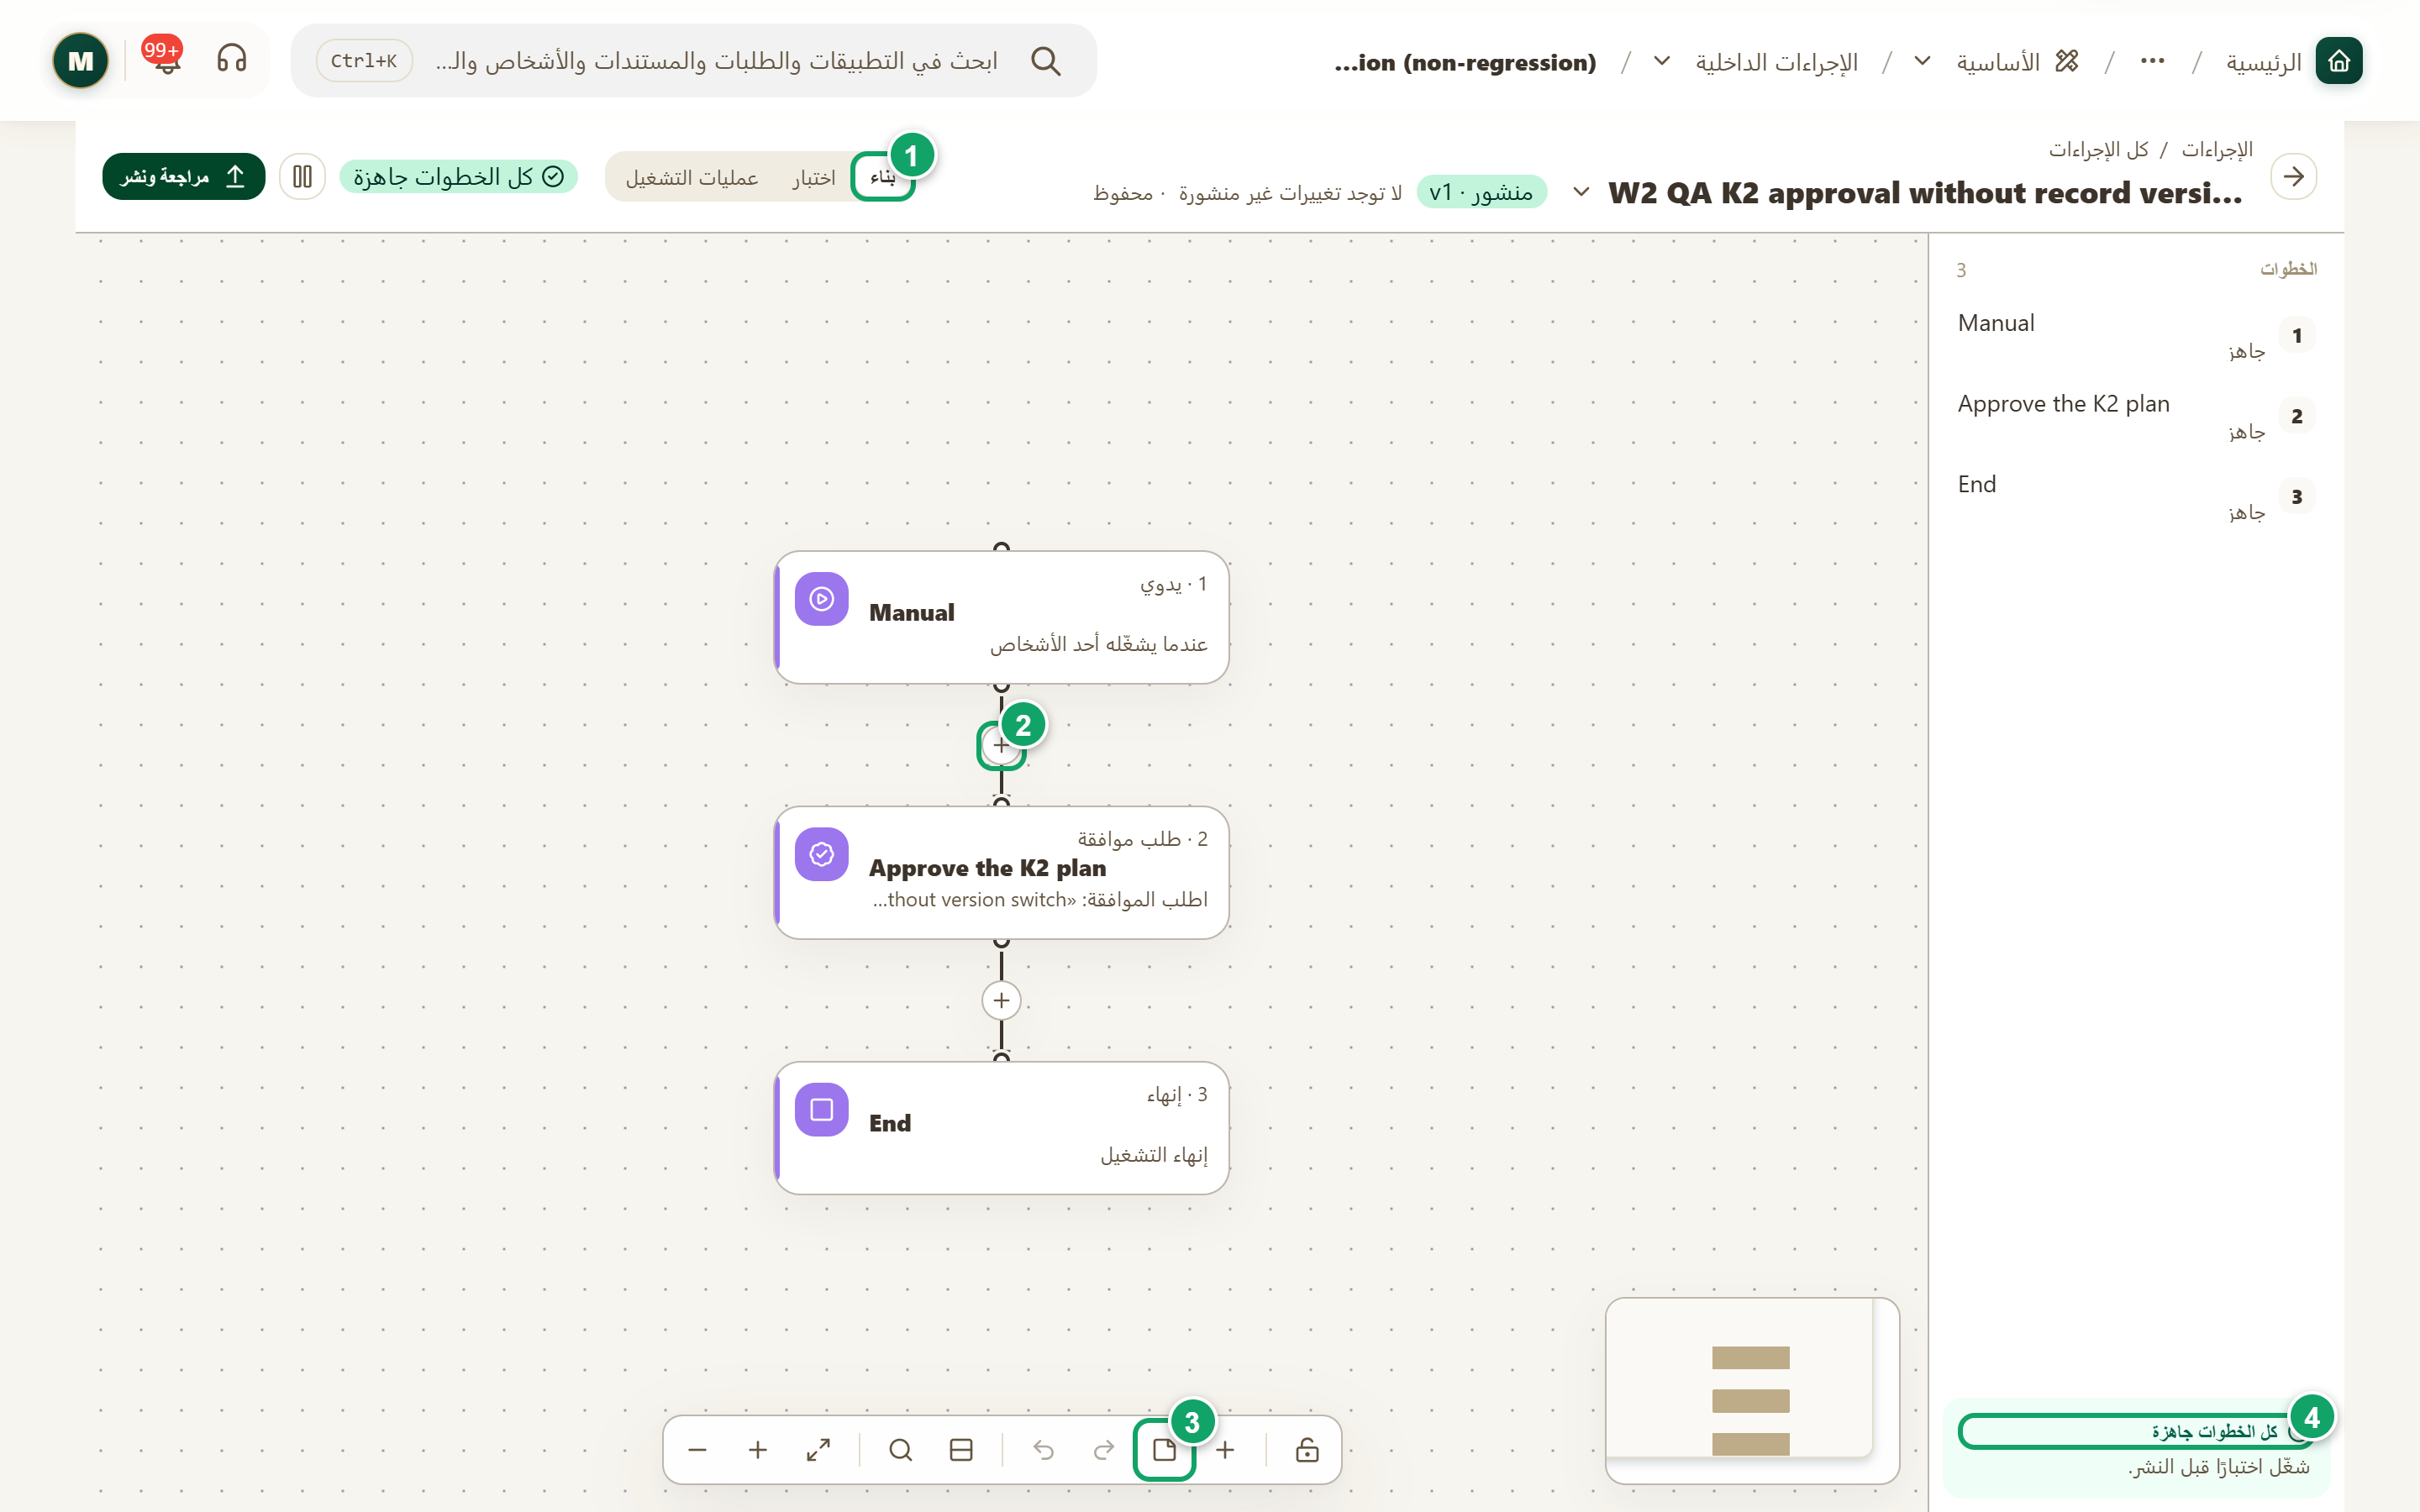
\includegraphics[width=0.95\linewidth,height=0.72\textheight,keepaspectratio]{figures/screens/ch06-isop-editor-ar.png}
\caption{محرر إجراء قائم في وضع «بناء»}
\label{fig:builder-isop-editor-screen}
\shotnote{تعرض الصورة إجراءً اختبارياً منشوراً في مؤسسة الاختبار، مفتوحاً في وضع «بناء» وكل خطواته جاهزة. ويجمع المحرر في شاشة واحدة قائمة الخطوات واللوحة وأدواتها، فتعرف حالة الإجراء قبل أن تعدّل فيه. ① «بناء»: الوضع الذي تعدّل فيه الخطوات. ② زر الإضافة «+» على الخط بين خطوتين: يفتح قائمة الخطوات. ③ «إضافة ملاحظة»: يضع على اللوحة ملاحظة لزملائك. ④ «كل الخطوات جاهزة»: ملخص قائمة الخطوات حين لا تحتاج أي خطوة إلى تهيئة.}
\end{figure}

\begin{table}[H]
\centering
\caption{أجزاء المحرر}
\label{tab:builder-isop-editor-parts}
\begin{tabularx}{\linewidth}{R{3.6cm} Y}
\rcHeaderRow
\thh{الجزء} & \thh{ما يقدمه}\\
رأس المحرر & «العودة إلى الإجراءات»، واسم الإجراء الذي يفتح تفاصيله وسجل إصداراته، وشارة الإصدار مثل «منشور · \en{v2}» أو «لم يُنشر بعد»، وحالة الحفظ مثل «محفوظ».\\
الأوضاع & «بناء» و«اختبار» و«عمليات التشغيل». ويظهر بجانبها اتصال الخادم: «متصل» أو «الخادم غير متصل».\\
شارة الجاهزية & «N للإصلاح» إذا بقيت خطوات ناقصة، أو «كل الخطوات جاهزة». والضغط عليها يفتح المراجعة.\\
الخطوات & قائمة مرقّمة بترتيب الخطوات، وتحت كل خطوة حالتها، مثل «جاهز» أو «يحتاج إلى تهيئة». وفوقها ملخص «خطوات تحتاج إلى تهيئة: N» أو «كل الخطوات جاهزة».\\
اللوحة & تضيف خطوة بزر الإضافة على الخط بين خطوتين، وتفتح قائمة الخطوة بالنقر بالزر الأيمن لنسخها أو لصقها أو اختبارها أو حذفها.\\
أدوات اللوحة & «إضافة مشغّل»، و«إضافة ملاحظة»، والتخطيط الأفقي أو العمودي، والتكبير والتصغير، و«ملاءمة سير العمل للعرض»، والبحث في الخطوات، والخريطة المصغرة، و«تراجع» و«إعادة».\\
\end{tabularx}
\end{table}

\subsection{إضافة خطوة}

عندما تضغط زر الإضافة تظهر قائمة الخطوات مقسّمة إلى أربع فئات: «تدفق التحكم» و«Kayan» و«خدمات المتعاملين» و«التكاملات». وتنقسم فئة «Kayan» إلى أقسام، مثل «السجلات» و«النماذج» و«المهام والمشاريع» و«الموافقات والطلبات» و«الإشعارات والمحادثات» و«المستندات». ويمكنك أن تبحث مباشرة في «ابحث عن التطبيقات والإجراءات» بدلاً من التنقل بين الفئات.

\begin{figure}[H]
\centering
\begin{tikzpicture}[node distance=0.5cm]
\node[stepBox] (a) {\RL{فتح الإجراء في وضع بناء}};
\node[stepBox,below=of a] (b) {\RL{إضافة خطوة من القائمة}};
\node[stepBox,below=of b] (c) {\RL{إعداد الخطوة}};
\node[stepBox,below=of c] (d) {\RL{مراجعة قائمة الخطوات}};
\node[stepBox,below=of d] (e) {\RL{الانتقال إلى اختبار}};
\draw[flowsTo] (a) -- (b);
\draw[flowsTo] (b) -- (c);
\draw[flowsTo] (c) -- (d);
\draw[flowsTo] (d) -- (e);
\end{tikzpicture}
\rclegend
\caption{جلسة بناء في المحرر}
\label{fig:builder-isop-editor-flow}
\shotnote{يوضح المخطط أن إضافة الخطوة وإعدادها عمل واحد يتكرر حتى تكتمل كل الخطوات. وتأتي مراجعة قائمة «الخطوات» قبل الاختبار، لأنها تكشف الخطوات الناقصة التي قد يتوقف عندها الاختبار.}
\end{figure}

\subsection{خطوات العمل والتحقق}
\begin{enumerate}
\item افتح الإجراء من «الإجراءات الداخلية»، وتأكد أن الوضع «بناء».
\item اضغط زر الإضافة على الخط بعد المشغّل، واختر الخطوة من فئتها أو بالبحث.
\item اضغط الخطوة على اللوحة لتفتح إعدادها، وأكمل حقولها المطلوبة.
\item أضف ملاحظة من «إضافة ملاحظة» إذا أردت أن تشرح جزءاً من المسار لزملائك.
\item راجع ملخص قائمة «الخطوات» حتى يظهر «كل الخطوات جاهزة».
\end{enumerate}

\textbf{تحقق ومعالجة المشكلة:} يجب أن تتغير حالة الحفظ إلى «محفوظ» بعد كل تعديل، وأن تظهر الخطوة الجديدة في قائمة «الخطوات» برقمها. فإذا حذفت خطوة بالخطأ، فاضغط «تراجع» أو \en{Ctrl+Z}. وإذا ظهر «الخادم غير متصل»، فتستطيع التعديل، لكنك لن تستطيع الاختبار أو النشر حتى يعود الاتصال.

\clearpage
\section{المشغّلات: ما الذي يبدأ الإجراء؟}
\label{sec:builder-feature-isop-triggers}

المشغّل هو الحدث الذي يبدأ عملية تشغيل جديدة للإجراء، وهو دائماً الخطوة الأولى في المسار. فقد يكون حدثاً في النظام مثل إنشاء سجل أو إرسال نموذج، أو موعداً متكرراً، أو ضغطة من أحد الأعضاء. ولا يعمل المشغّل إلا بعد نشر الإجراء، ويمكن أن يحتوي الإجراء على أكثر من مشغّل.

\textbf{المسار ومن يستخدمه:} لوحة «إجراء جديد» ← «ما الذي يبدأه؟» ← «مزيد من المُشغِّلات»، أو في المحرر «إضافة مشغّل»، أو «تغيير المشغّل» من إعداد خطوة المشغّل. يستخدمها من يبني الإجراء.

\begin{rcnote}[مثال: شركة الأفق]
يختار المسؤول «إنشاء سجل جديد» (④)، ثم يحدد في «الجدول» نوع السجلات «طلبات الزيارة». فكلما أضاف عمر حداد طلباً جديداً مثل \en{HZN-VR-0001}، بدأت عملية تشغيل جديدة للإجراء.
\end{rcnote}

\begin{figure}[H]
\centering
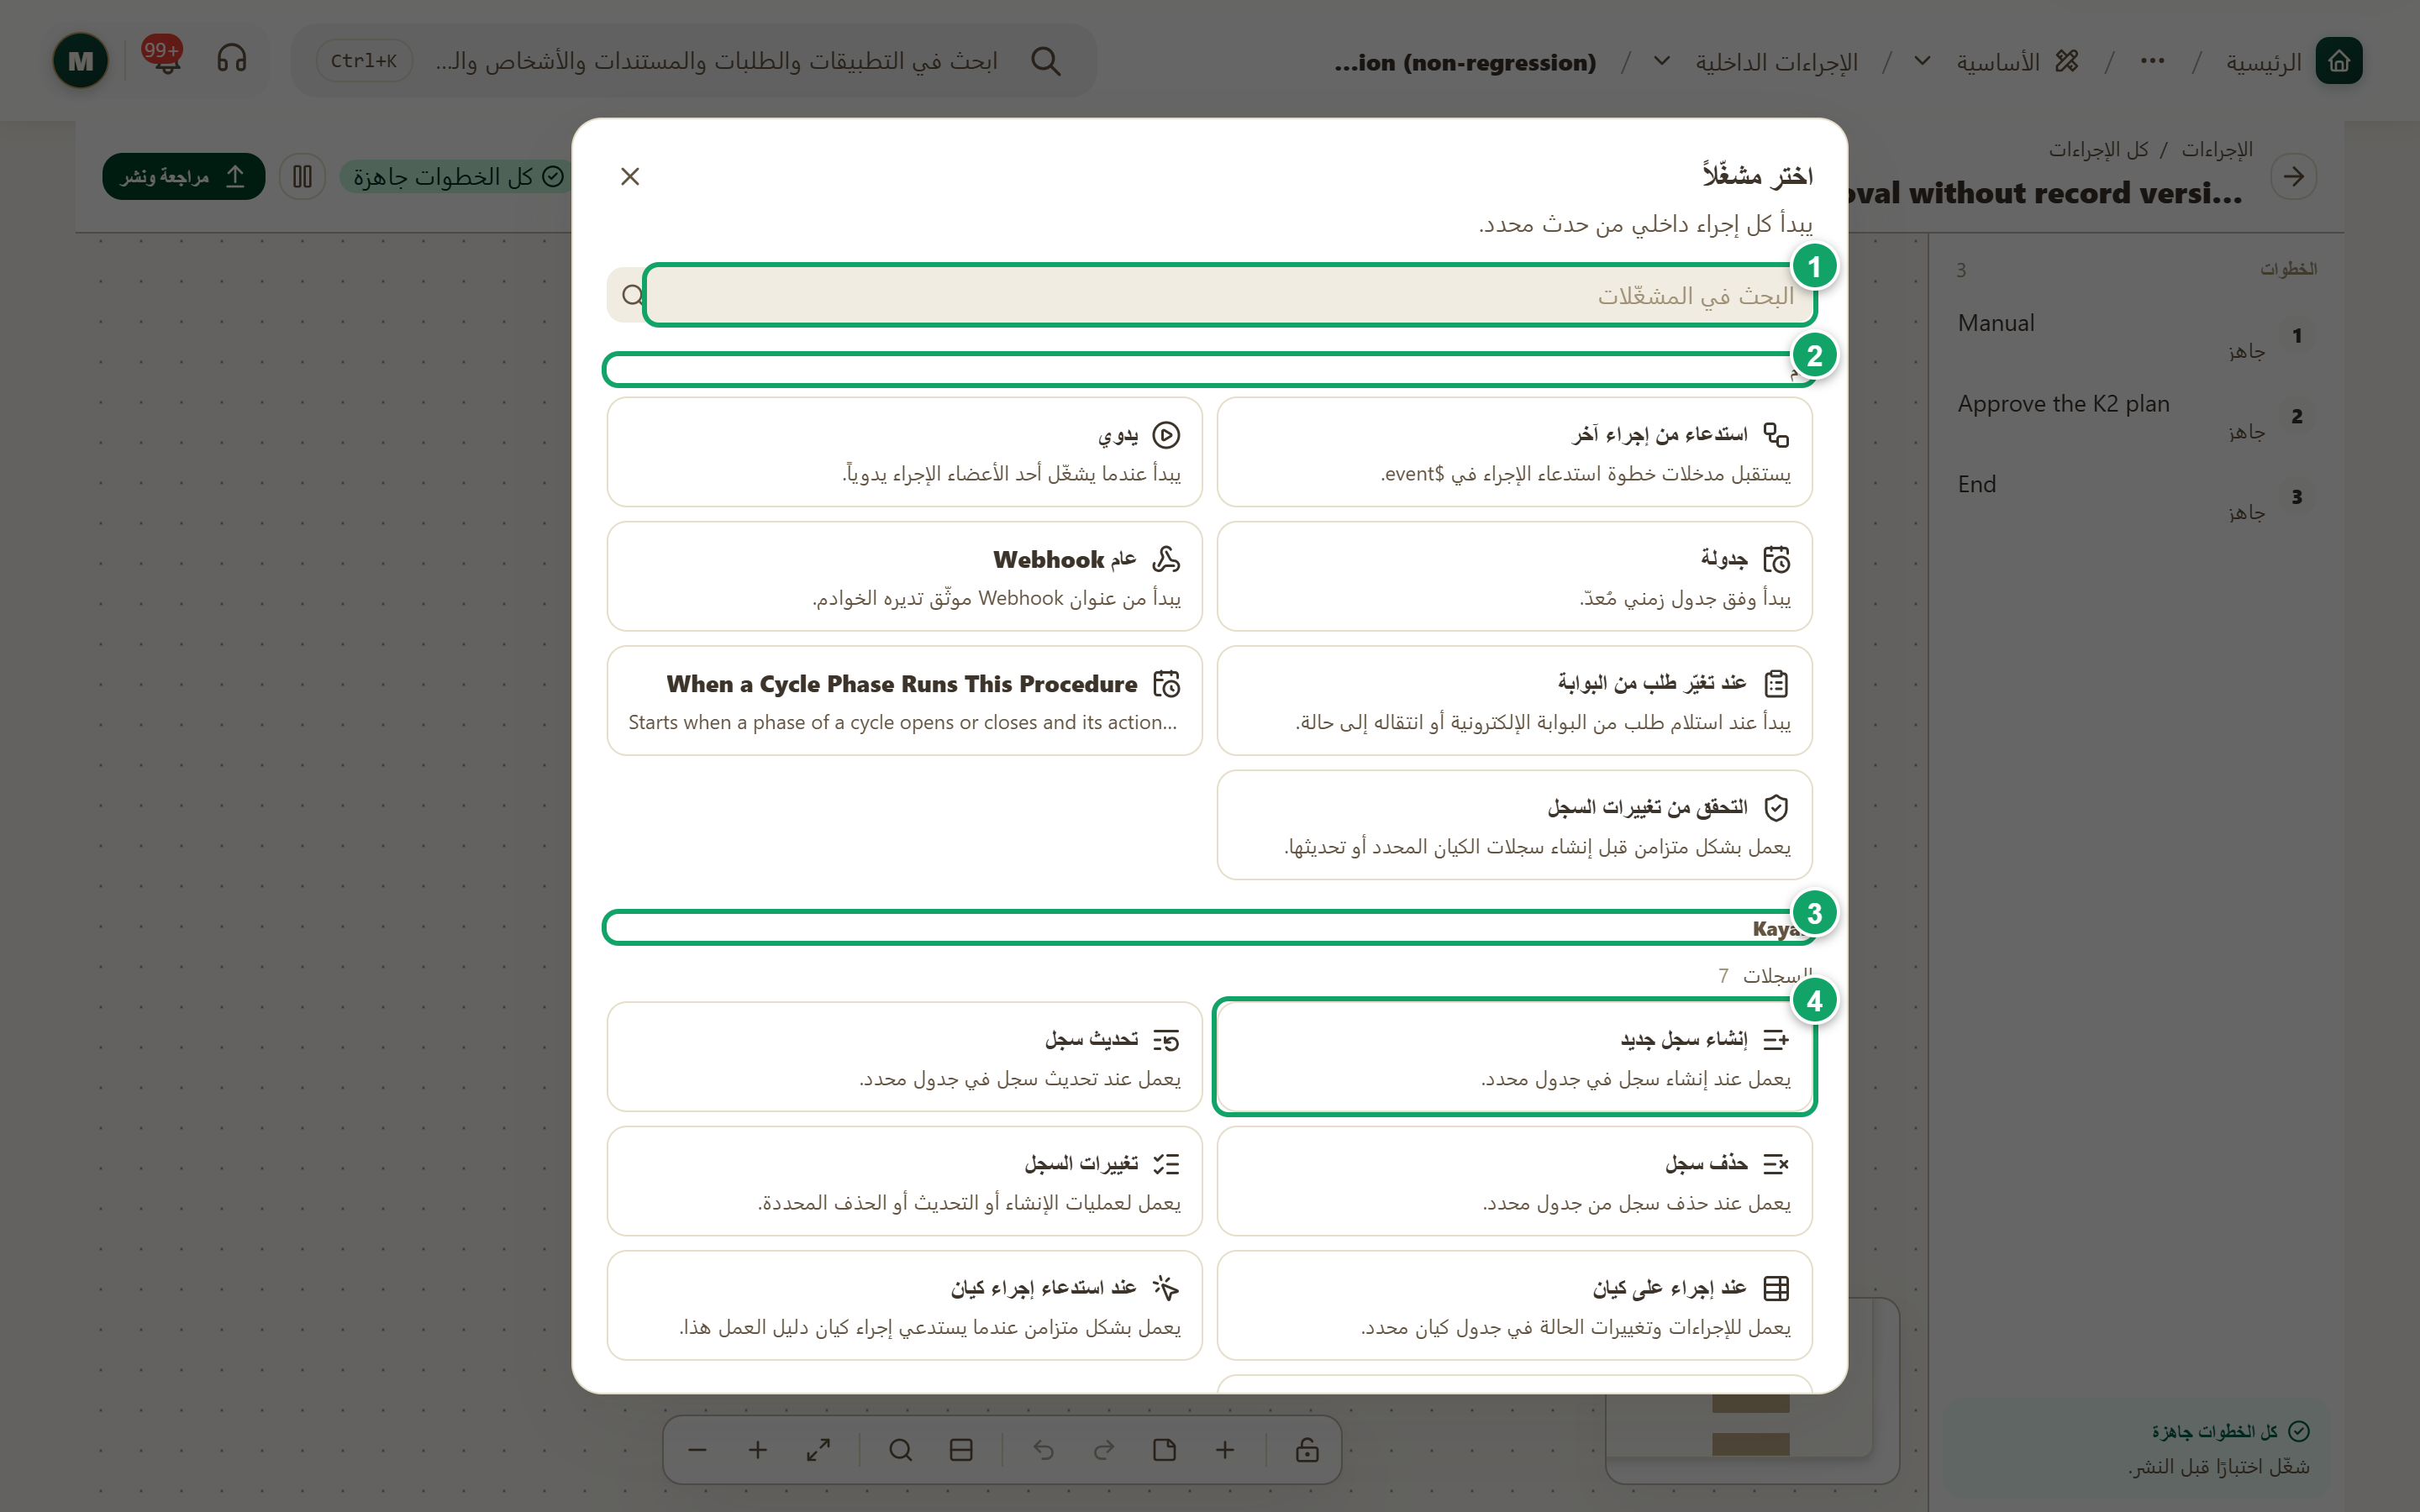
\includegraphics[width=0.95\linewidth,height=0.72\textheight,keepaspectratio]{figures/screens/ch06-isop-triggers-ar.png}
\caption{نافذة «اختر مشغّلاً»}
\label{fig:builder-isop-triggers-screen}
\shotnote{تعرض الصورة النافذة التي تفتح من «إضافة مشغّل»، وفيها المشغّلات مجمّعة تحت «عام» ثم «Kayan» مقسّمة إلى أقسام، وتليها مشغّلات التكاملات عند التمرير. وتفيدك المجموعات في الوصول إلى الحدث المناسب دون حفظ أسماء المشغّلات كلها. ① «البحث في المشغّلات»: تكتب فيه اسم الحدث مباشرة. ② «عام»: المشغّلات اليدوية والمجدولة والمستدعاة. ③ «Kayan»: أحداث النظام مقسّمة حسب القسم. ④ «إنشاء سجل جديد»: مثال على مشغّل يعمل عند إنشاء سجل في جدول تختاره.}
\end{figure}

\begin{table}[H]
\centering
\caption{مجموعات المشغّلات في نافذة «اختر مشغّلاً»}
\label{tab:builder-isop-triggers-groups}
\begin{tabularx}{\linewidth}{R{3.6cm} Y}
\rcHeaderRow
\thh{المجموعة} & \thh{أمثلة ومتى تستخدمها}\\
عام & «يدوي» عندما يشغّل أحد الأعضاء الإجراء بنفسه، و«جدولة» لموعد يومي أو أسبوعي أو بتعبير \en{Cron}، و«Webhook عام» عندما يستدعي نظام آخر رابط الإجراء، و«استدعاء من إجراء آخر» للإجراء الذي تستدعيه خطوة من إجراء آخر. ويوجد كذلك مشغّل يبدأ الإجراء عندما تفتح مرحلة من «الدورات» أو تُغلق وتسمّي الإجراء في إجراءاتها.\\
\en{Kayan} & أحداث النظام مقسّمة حسب القسم، كالسجلات والنماذج والمهام والموافقات والملفات والدعم والبريد وواتساب.\\
التكاملات & أحداث من خدمات خارجية، وتحتاج عادةً إلى اتصال بحساب تلك الخدمة.\\
\end{tabularx}
\end{table}

\begin{table}[H]
\centering
\caption{مشغّلات السجلات والنماذج والمهام والموافقات}
\label{tab:builder-isop-triggers-kayan}
\begin{tabularx}{\linewidth}{R{3.6cm} Y}
\rcHeaderRow
\thh{المشغّل} & \thh{متى يبدأ الإجراء}\\
إنشاء سجل جديد، تحديث سجل، حذف سجل & عند إنشاء سجل أو تحديثه أو حذفه في «الجدول» الذي تختاره. أما «تغييرات السجل» فيجمع العمليات التي تحددها منها.\\
عند إجراء على كيان & عند تنفيذ إجراء أو تغيير حالة في نوع سجلات محدد، مثل انتقال الطلب إلى حالة الاعتماد.\\
عند إرسال نموذج & عند إرسال أي جلسة نموذج في النظام.\\
عند إجراء على نموذج & عندما ينفّذ نموذج محدد أحد الإجراءات التي تختارها.\\
عند إجراء على مهمة & عند تنفيذ إجراءات مهمة أو تغيّر حالتها. ويوجد مشغّل مستقل عند إضافة تعليق إلى مهمة.\\
عند استجابة موافقة، عند انتهاء موافقة & الأول مع كل رد على طلب موافقة، والثاني عندما يكتمل الطلب أو يُلغى أو تنتهي مهلته.\\
\end{tabularx}
\end{table}

\begin{rcwarn}[تغيير المشغّل يحذف إعداده]
إذا ضغطت «تغيير المشغّل» بعد إعداده، تظهر رسالة «هل تريد تغيير المشغّل؟» مع قائمة الحقول التي ستُحذف. فاضغط «متابعة» فقط إذا كنت ستعيد إعداد المشغّل الجديد.
\end{rcwarn}

\begin{figure}[H]
\centering
\begin{tikzpicture}[node distance=0.5cm]
\node[stepBox] (a) {\RL{اختر مشغّلاً}};
\node[stepBox,below=of a] (b) {\RL{البحث أو اختيار المجموعة}};
\node[stepBox,below=of b] (c) {\RL{إعداد حقول المشغّل}};
\node[stepBox,below=of c] (d) {\RL{إضافة خطوة بعده}};
\node[stepBox,below=of d] (e) {\RL{النشر ليبدأ العمل}};
\draw[flowsTo] (a) -- (b);
\draw[flowsTo] (b) -- (c);
\draw[flowsTo] (c) -- (d);
\draw[flowsTo] (d) -- (e);
\end{tikzpicture}
\rclegend
\caption{إعداد المشغّل}
\label{fig:builder-isop-triggers-flow}
\shotnote{يربط المخطط بين المشغّل والنشر، لأن المشغّل في المسودة لا يبدأ أي عملية تشغيل. ويذكّرك بإضافة خطوة بعده، فالمراجعة ترفض النشر برسالة «أضف خطوة بعد هذا المُشغِّل» إذا بقي وحده.}
\end{figure}

\subsection{خطوات العمل والتحقق}
\begin{enumerate}
\item في المحرر، اضغط «إضافة مشغّل»، أو افتح المشغّل الحالي واضغط «تغيير المشغّل».
\item ابحث في «البحث في المشغّلات» باسم الحدث، أو تصفح «عام» و\en{Kayan} و«التكاملات».
\item اختر المشغّل، ثم أكمل حقوله، مثل «الجدول» لمشغّلات السجلات أو التكرار والوقت والمنطقة الزمنية لـ«جدولة».
\item أضف خطوة بعد المشغّل، ثم انشر الإجراء.
\end{enumerate}

\textbf{تحقق ومعالجة المشكلة:} بعد النشر يجب أن تظهر عملية تشغيل جديدة في «عمليات التشغيل» كلما وقع الحدث. فإذا لم تظهر، فتأكد أن الإجراء ليس «متوقفاً مؤقتاً»، وأنك اخترت الجدول أو النموذج الصحيح في المشغّل. ولمشغّل «Webhook عام» يظهر «رابط الويب هوك المنشور» بعد النشر فقط.

\clearpage
\section{خطوات التحكم في المسار}
\label{sec:builder-feature-isop-control-flow}

خطوات التحكم لا تنفّذ عملاً في النظام، بل تحدد طريق الإجراء: هل يتفرّع؟ هل يكرر خطوة لكل عنصر في قائمة؟ هل ينتظر مدة أو حدثاً؟ متى ينتهي؟ وتجدها كلها في فئة «تدفق التحكم» عند إضافة خطوة. وبفضلها يتبع الإجراء القاعدة التي تعمل بها المؤسسة فعلاً، لا مساراً واحداً ثابتاً.

\textbf{المسار ومن يستخدمه:} المحرر ← زر الإضافة ← «تدفق التحكم». يستخدمها من يبني الإجراء.

\begin{rcnote}[مثال: شركة الأفق]
يضيف المسؤول بعد «طلب موافقة» خطوة «تفرّع شرطي» (②) لها مساران: الأول يتابع إلى إنشاء مهمة عمر إذا كانت النتيجة موافقة، والثاني ينتهي بخطوة «إنهاء» إذا طلبت سارة تغييرات.
\end{rcnote}

\begin{figure}[H]
\centering
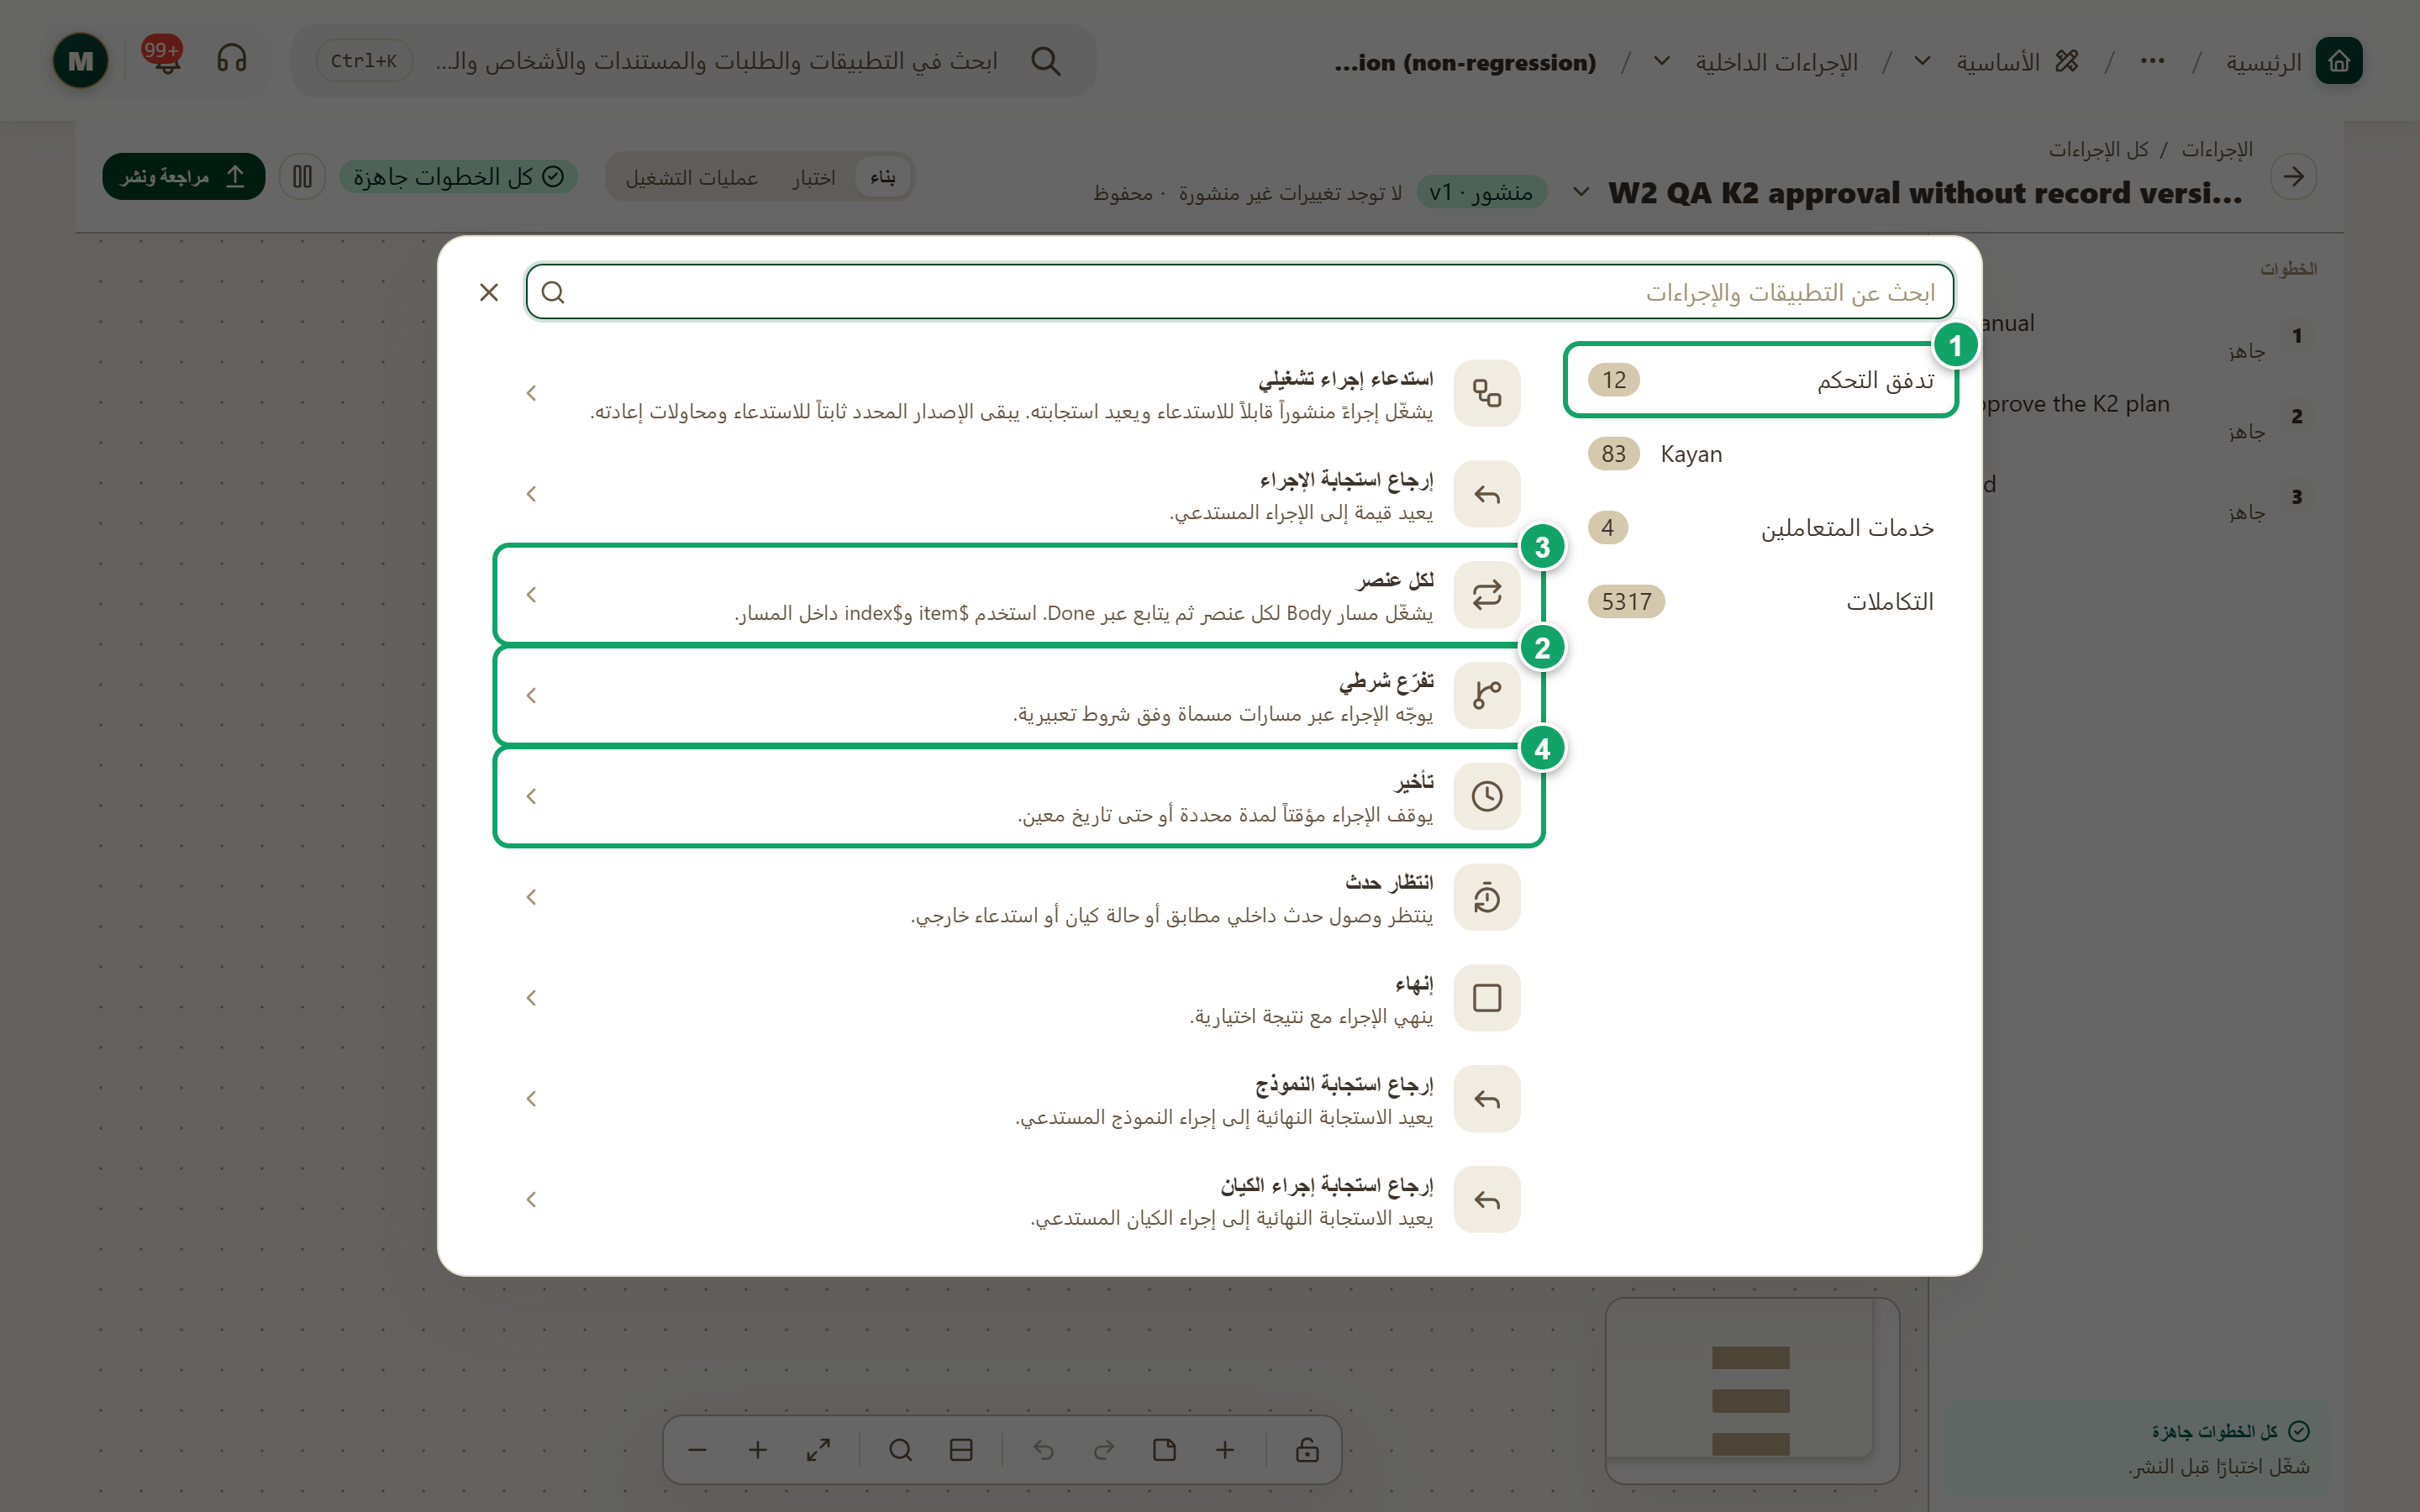
\includegraphics[width=0.95\linewidth,height=0.72\textheight,keepaspectratio]{figures/screens/ch06-isop-control-flow-ar.png}
\caption{فئة «تدفق التحكم» في قائمة الخطوات}
\label{fig:builder-isop-control-flow-screen}
\shotnote{تعرض الصورة قائمة الخطوات بعد الضغط على زر الإضافة، وقد فُتحت على فئة «تدفق التحكم» بخطواتها الاثنتي عشرة ووصف مختصر لكل منها. ويساعدك الوصف على اختيار الخطوة التي تحدد طريق الإجراء قبل أن تضيفها. ① «تدفق التحكم»: الفئة التي تجمع خطوات التحكم. ② «تفرّع شرطي»: يوجّه الإجراء إلى مسارات مسمّاة. ③ «لكل عنصر»: يكرر خطوات لكل عنصر في قائمة. ④ «تأخير»: يوقف الإجراء مدة محددة أو حتى تاريخ.}
\end{figure}

\begin{table}[H]
\centering
\caption{خطوات «تدفق التحكم»}
\label{tab:builder-isop-control-flow-steps}
\begin{tabularx}{\linewidth}{R{3.6cm} Y}
\rcHeaderRow
\thh{الخطوة} & \thh{ما تفعله}\\
تفرّع شرطي & يوجّه الإجراء إلى مسارات مسمّاة، لكل مسار تسمية وشرط. وتبدأ بمسارين ومسار بديل عند عدم المطابقة، وتختار في «المسارات المطابقة» بين «أول مسار مطابق» و«كل المسارات المطابقة».\\
لكل عنصر & يكرر خطوات جسم الحلقة لكل عنصر في «العناصر»، ثم يتابع بعد انتهائها. وداخل الحلقة تستطيع استخدام العنصر الحالي وموضعه.\\
تأخير & يوقف الإجراء «لمدة محددة» مثل يوم واحد، أو «حتى تاريخ معين».\\
انتظار حدث & ينتظر حتى يصل حدث داخلي أو حالة سجل أو استدعاء خارجي يطابق ما تحدده، مع مهلة اختيارية.\\
إنهاء & ينهي التشغيل مع نتيجة اختيارية، ولا يمكن أن تتبعه أي خطوة.\\
استدعاء إجراء تشغيلي & يشغّل إجراءً منشوراً مشغّله «استدعاء من إجراء آخر»، وينتظر استجابته. ويثبت الإصدار المختار للاستدعاء نفسه حتى عند إعادة المحاولة.\\
إرجاع استجابة الإجراء & يعيد قيمة إلى الإجراء الذي استدعى هذا الإجراء.\\
تشغيل \en{JavaScript} & يشغّل شيفرة قصيرة في بيئة معزولة دون شبكة، ويعيد قيمة تستخدمها الخطوات التالية.\\
\end{tabularx}
\end{table}

\begin{rcwarn}[القرار وحده يتفرّع]
لا يمكن أن تخرج من خطوة عادية إلا وصلة واحدة. فإذا أردت مسارين، فأضف «تفرّع شرطي»، وإلا ظهرت مشكلة «القرار وحده يمكنه التفرّع إلى عدة مسارات». وكذلك يجب أن يحمل كل مسار في القرار اسماً.
\end{rcwarn}

\begin{figure}[H]
\centering
\begin{tikzpicture}[node distance=0.5cm]
\node[stepBox] (a) {\RL{خطوة سابقة تعيد نتيجة}};
\node[stepBox,below=of a] (b) {\RL{تفرّع شرطي}};
\node[stepBox,below=of b] (c) {\RL{المسار المطابق}};
\node[stepBox,below=of c] (d) {\RL{تأخير أو انتظار حدث}};
\node[stepBox,below=of d] (e) {\RL{إنهاء}};
\draw[flowsTo] (a) -- (b);
\draw[flowsTo] (b) -- (c);
\draw[flowsTo] (c) -- (d);
\draw[flowsTo] (d) -- (e);
\end{tikzpicture}
\rclegend
\caption{كيف تقود خطوات التحكم المسار}
\label{fig:builder-isop-control-flow-flow}
\shotnote{يبيّن المخطط أن القرار يعتمد على نتيجة خطوة سبقته، فلا معنى لشرط لا يجد بيانات يقرؤها. أما التأخير والانتظار فيجعلان التشغيل في حالة «بانتظار استجابة» حتى يحين الموعد أو يصل الحدث، ثم يتابع المسار حتى «إنهاء».}
\end{figure}

\subsection{خطوات العمل والتحقق}
\begin{enumerate}
\item أضف «تفرّع شرطي» بعد الخطوة التي تريد أن تقرر بناءً على نتيجتها.
\item في إعداد القرار، اكتب تسمية كل مسار، واضغط «حدّد الشرط» لتكتب الشرط أو تختار «دائمًا» أو «أبدًا».
\item اضغط «إضافة مسار» إذا احتجت مساراً آخر، واختر في «المسارات المطابقة» طريقة الاختيار.
\item أضف إلى نهاية كل مسار الخطوة التالية أو خطوة «إنهاء».
\end{enumerate}

\textbf{تحقق ومعالجة المشكلة:} يجب أن ترى على اللوحة خطاً لكل مسار يحمل تسميته، وأن يختفي تنبيه «شروط القرار لا تطابق مساراته». وإذا سلك الاختبار المسار الخطأ، فافتح نتيجة الخطوة السابقة في الاختبار وتحقق من القيمة التي يقرؤها الشرط.

\clearpage
\section{خطوات السجلات والنماذج}
\label{sec:builder-feature-isop-records}

تتعامل هذه الخطوات مع البيانات المحفوظة في أنواع السجلات ومع النماذج. فتستطيع بها أن تبحث عن سجلات، أو تُنشئ سجلاً، أو تحدّث حقول سجل موجود، أو تطلب من الأعضاء تعبئة نموذج. وتجدها في فئة \en{Kayan} ضمن قسمي «السجلات» و«النماذج».

\textbf{المسار ومن يستخدمه:} المحرر ← زر الإضافة ← \en{Kayan} ← «السجلات» أو «النماذج». يستخدمها من يبني الإجراء، ويحتاج إلى صلاحية على أنواع السجلات التي تتعامل معها الخطوة.

\begin{rcnote}[مثال: شركة الأفق]
يضيف المسؤول خطوة «تحديث سجل كيان» (⑤) بعد موافقة سارة الخطيب، فيختار نوع السجلات «طلبات الزيارة» ويضع في «السجل» السجل الذي بدأ التشغيل، ثم يعيّن حالة الطلب إلى معتمد.
\end{rcnote}

\begin{figure}[H]
\centering
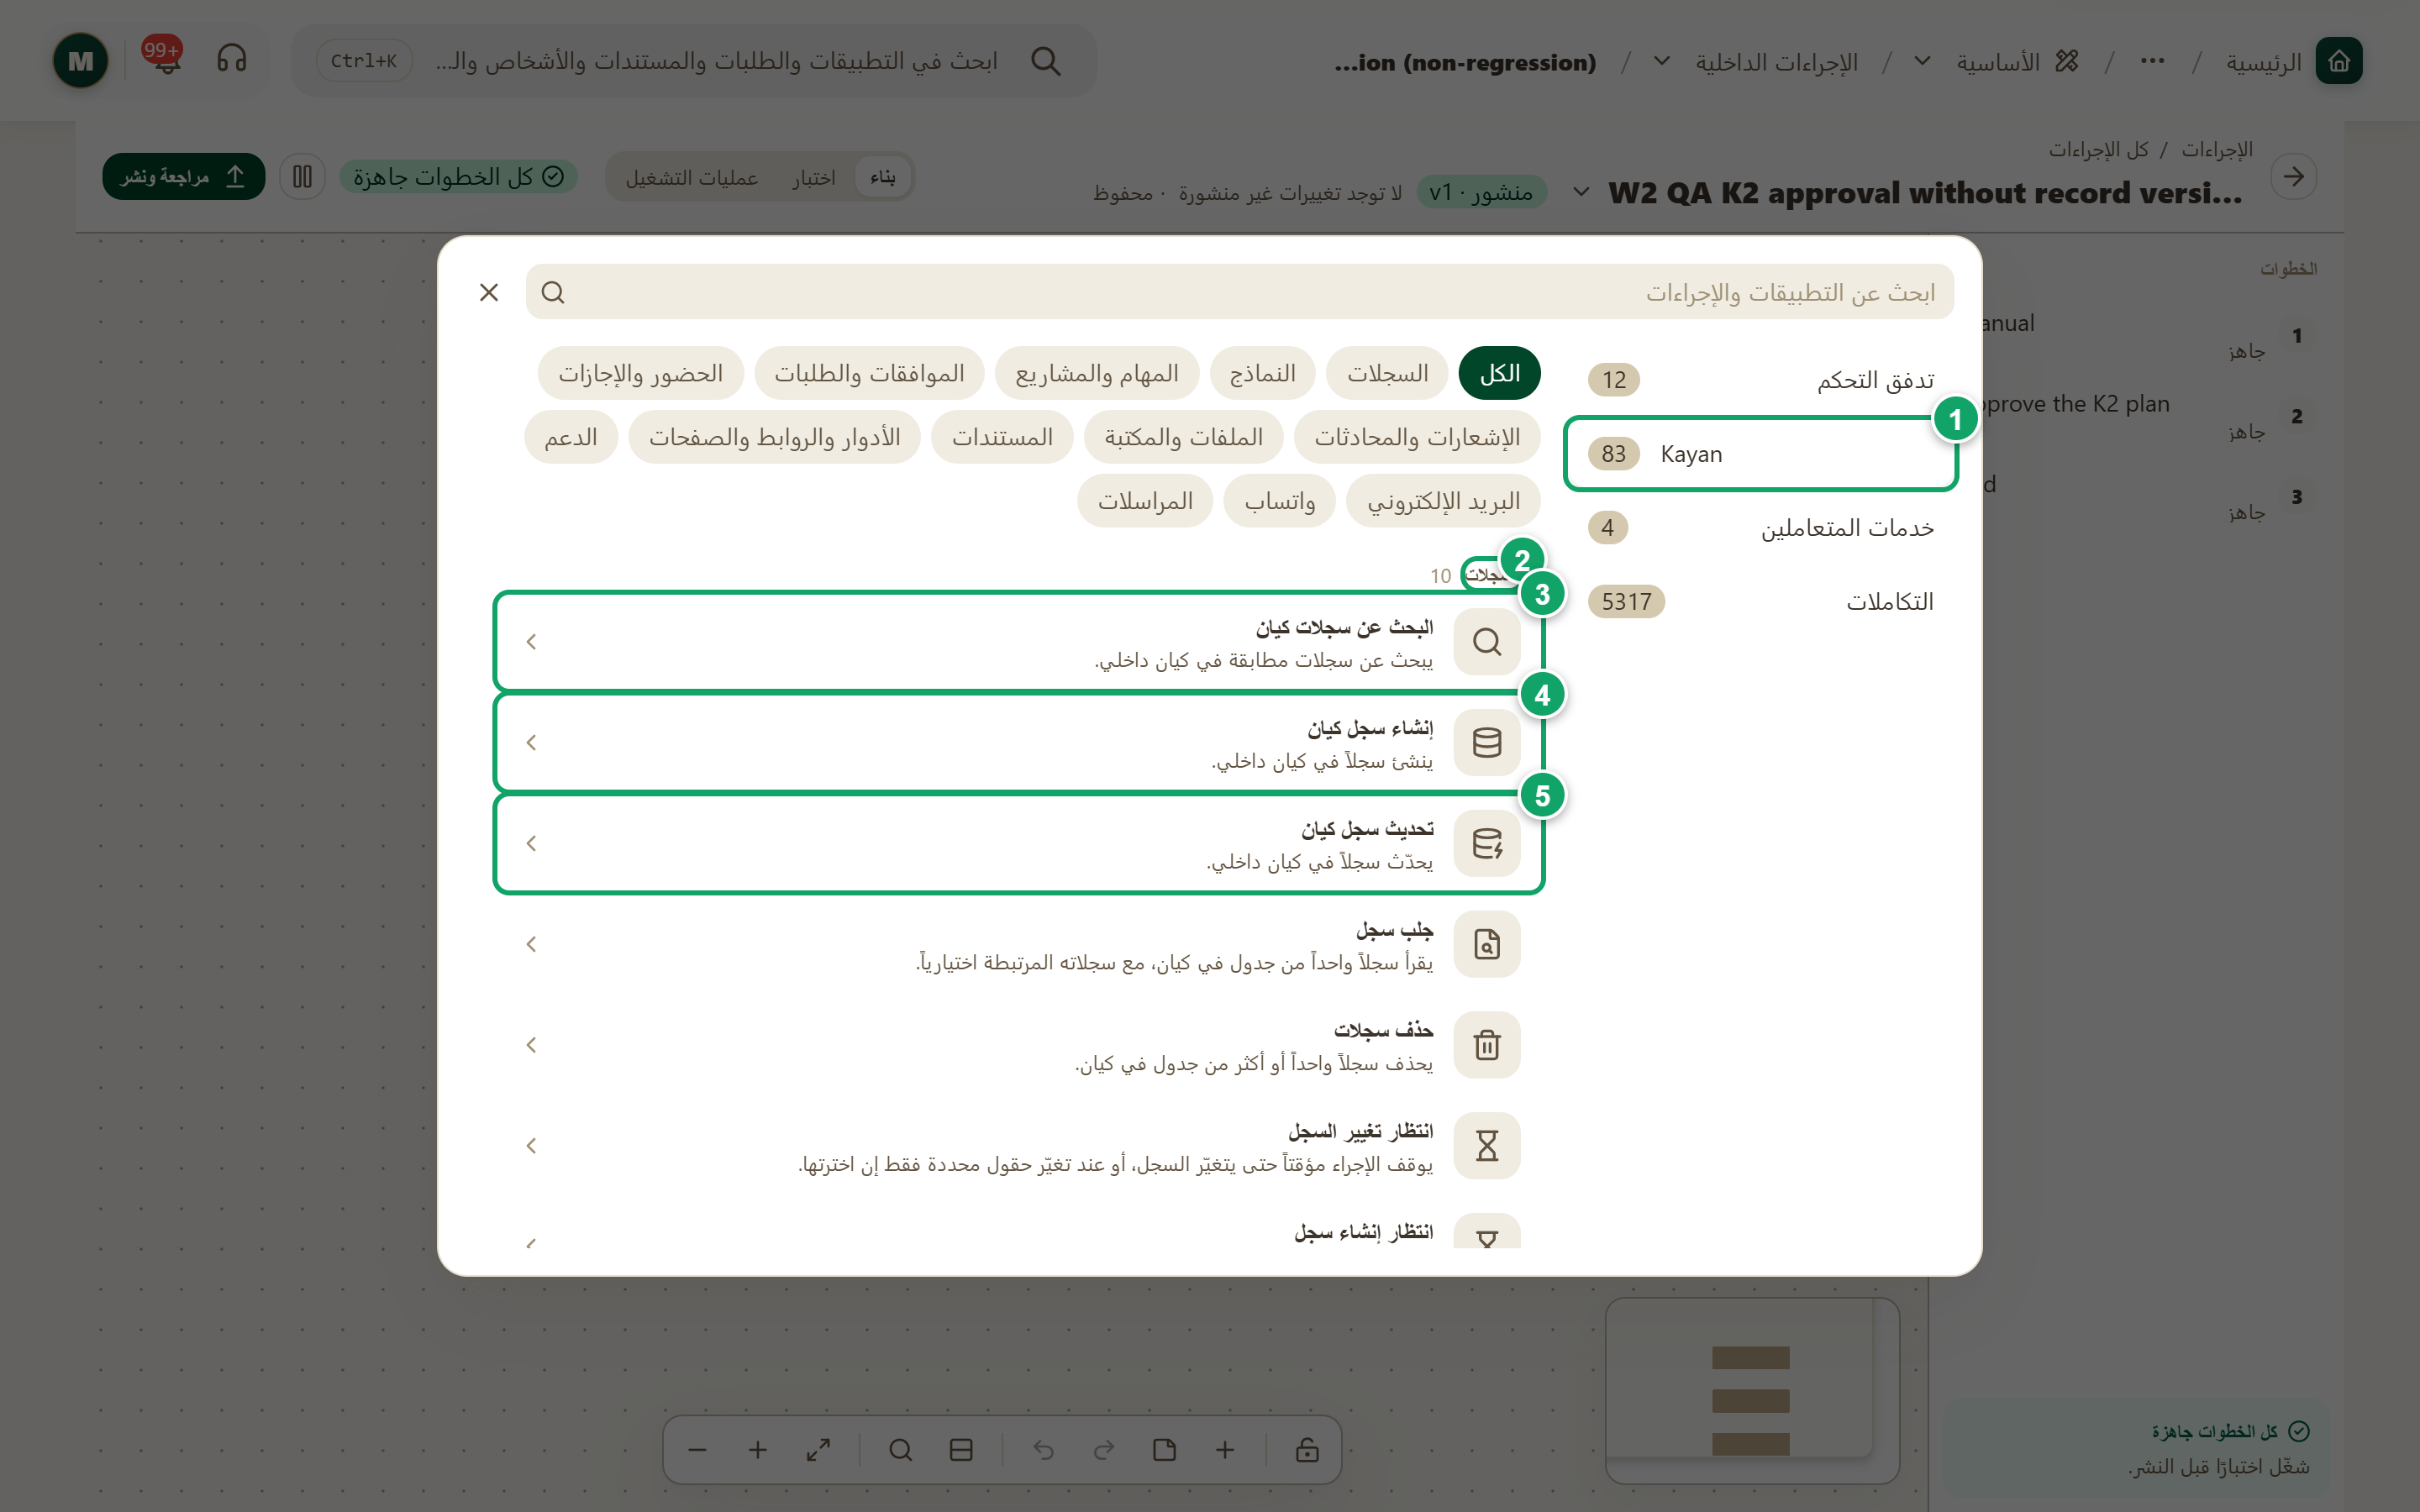
\includegraphics[width=0.95\linewidth,height=0.72\textheight,keepaspectratio]{figures/screens/ch06-isop-records-ar.png}
\caption{قسم «السجلات» في فئة «Kayan»}
\label{fig:builder-isop-records-screen}
\shotnote{تعرض الصورة فئة «Kayan» في قائمة الخطوات، وفيها أزرار الأقسام ثم خطوات قسم «السجلات». ويبيّن ذلك أن خطوات السجلات والنماذج كلها في فئة واحدة تصل إليها بزر القسم بدلاً من التمرير الطويل. ① «Kayan»: فئة خطوات النظام. ② «السجلات»: القسم الذي يجمع خطوات السجلات. ③ «البحث عن سجلات كيان»: يعيد السجلات المطابقة لشروطك. ④ «إنشاء سجل كيان»: ينشئ سجلاً جديداً. ⑤ «تحديث سجل كيان»: يعدّل حقول سجل قائم.}
\end{figure}

\begin{table}[H]
\centering
\caption{خطوات السجلات}
\label{tab:builder-isop-records-steps}
\begin{tabularx}{\linewidth}{R{3.6cm} Y}
\rcHeaderRow
\thh{الخطوة} & \thh{ما تفعله وأهم حقولها}\\
البحث عن سجلات كيان & تعيد السجلات المطابقة لشروطك في «الكيان» المختار، مع الحقول التي تحددها وعدد أقصى بين 1 و1000.\\
إنشاء سجل كيان & تُنشئ سجلاً وتملأ «قيم الحقول» «حقل بحقل» أو «كائن كامل». ويحدد «إذا وُجد سجل مطابق» ما يحدث عند التكرار: «إيقاف بخطأ» أو «تخطٍّ» أو «استخدام الموجود».\\
تحديث سجل كيان & تحدّث حقول «السجل» الذي تختاره أو الذي يأتي من المشغّل.\\
جلب سجل، حذف سجلات & تقرأ سجلاً واحداً لتستخدم قيمه، أو تحذف سجلات.\\
انتظار تغيير السجل، انتظار إنشاء سجل & توقف الإجراء حتى يتغير سجل أو يُنشأ سجل يطابق الشرط.\\
تنفيذ إجراء كيان & تنفّذ إجراءً معرّفاً على نوع السجلات، مثل الانتقال إلى حالة.\\
\end{tabularx}
\end{table}

\begin{table}[H]
\centering
\caption{خطوات النماذج}
\label{tab:builder-isop-records-forms}
\begin{tabularx}{\linewidth}{R{3.6cm} Y}
\rcHeaderRow
\thh{الخطوة} & \thh{ما تفعله}\\
طلب نموذج & تطلب من الأعضاء المحددين في «المستلمون» تعبئة «النموذج» المختار، مع «تاريخ الاستحقاق» و«انتظار الاكتمال» و«مهلة الانتظار».\\
بدء جلسة نموذج & تبدأ جلسة تعبئة جديدة لنموذج.\\
جلب إرسال نموذج، البحث عن إرسالات النماذج & تقرأ ما أرسله الأعضاء لتستخدمه في الخطوات التالية.\\
حفظ النموذج بصيغة \en{PDF} & تحفظ الإرسال ملفاً بصيغة \en{PDF}.\\
\end{tabularx}
\end{table}

\begin{figure}[H]
\centering
\begin{tikzpicture}[node distance=0.5cm]
\node[stepBox] (a) {\RL{اختيار الكيان}};
\node[stepBox,below=of a] (b) {\RL{اختيار السجل أو الشروط}};
\node[stepBox,below=of b] (c) {\RL{تعيين قيم الحقول}};
\node[stepBox,below=of c] (d) {\RL{إضافة الحقول المطلوبة}};
\node[stepBox,below=of d] (e) {\RL{اختبار الخطوة}};
\draw[flowsTo] (a) -- (b);
\draw[flowsTo] (b) -- (c);
\draw[flowsTo] (c) -- (d);
\draw[flowsTo] (d) -- (e);
\end{tikzpicture}
\rclegend
\caption{إعداد خطوة سجل}
\label{fig:builder-isop-records-flow}
\shotnote{يبدأ المخطط باختيار الكيان لأن الحقول المتاحة تُحمَّل منه، فلا تستطيع اختيار السجل أو القيم قبله. ويضع إضافة الحقول المطلوبة قبل الاختبار، لأن الخطوة لا تكتمل حتى تعيّن قيماً لكل الحقول الإلزامية في نوع السجلات.}
\end{figure}

\subsection{خطوات العمل والتحقق}
\begin{enumerate}
\item أضف الخطوة من قسم «السجلات»، واختر «الكيان».
\item في خطوة التحديث، اختر «السجل»، أو استخدم السجل الذي جاء من المشغّل بدلاً من سجل ثابت.
\item في «قيم الحقول»، اضغط «إضافة قيمة» واختر الحقل ثم اكتب قيمته أو أدرجها من خطوة سابقة.
\item اضغط «إضافة الحقول المطلوبة» إذا ظهر، حتى تغطي كل الحقول الإلزامية.
\end{enumerate}

\textbf{تحقق ومعالجة المشكلة:} يجب أن يختفي من الخطوة تنبيه «عيّن قيمًا للحقول المطلوبة». فإذا ظهر «لا توجد حقول قابلة للكتابة لهذه العملية»، فتحقق من صلاحياتك على نوع السجلات. وإذا تجاوزت الخطوة حداً على السجلات، فاكتب «التبرير عند تجاوز حدّ» إن كان الحد يسمح بالتجاوز، وإلا توقف التشغيل.

\clearpage
\section{خطوات المهام والموافقات والإشعارات والمستندات}
\label{sec:builder-feature-isop-people}

هذه الخطوات تشرك الأشخاص في الإجراء: تُنشئ مهمة لعضو، أو تطلب موافقة أو توقيعاً، أو ترسل إشعاراً، أو تُنشئ مستنداً من قالب. وبعضها ينتظر رد الشخص قبل أن يتابع، فيبقى التشغيل في حالة «بانتظار استجابة» حتى يصل الرد أو تنتهي المهلة.

\textbf{المسار ومن يستخدمه:} المحرر ← زر الإضافة ← \en{Kayan} ← «المهام والمشاريع» أو «الموافقات والطلبات» أو «الإشعارات والمحادثات» أو «المستندات». يستخدمها من يبني الإجراء.

\begin{rcnote}[مثال: شركة الأفق]
يضيف المسؤول «طلب موافقة» (⑤) بعنوان «اعتماد زيارة فرع حلب» وتكون سارة الخطيب في مرحلته الوحيدة. وبعد موافقتها تُنشئ خطوة «إنشاء مهمة» مهمة «تجهيز الزيارة» وتضيف عمر حداد إلى حقل «المكلّفون».
\end{rcnote}

\begin{figure}[H]
\centering
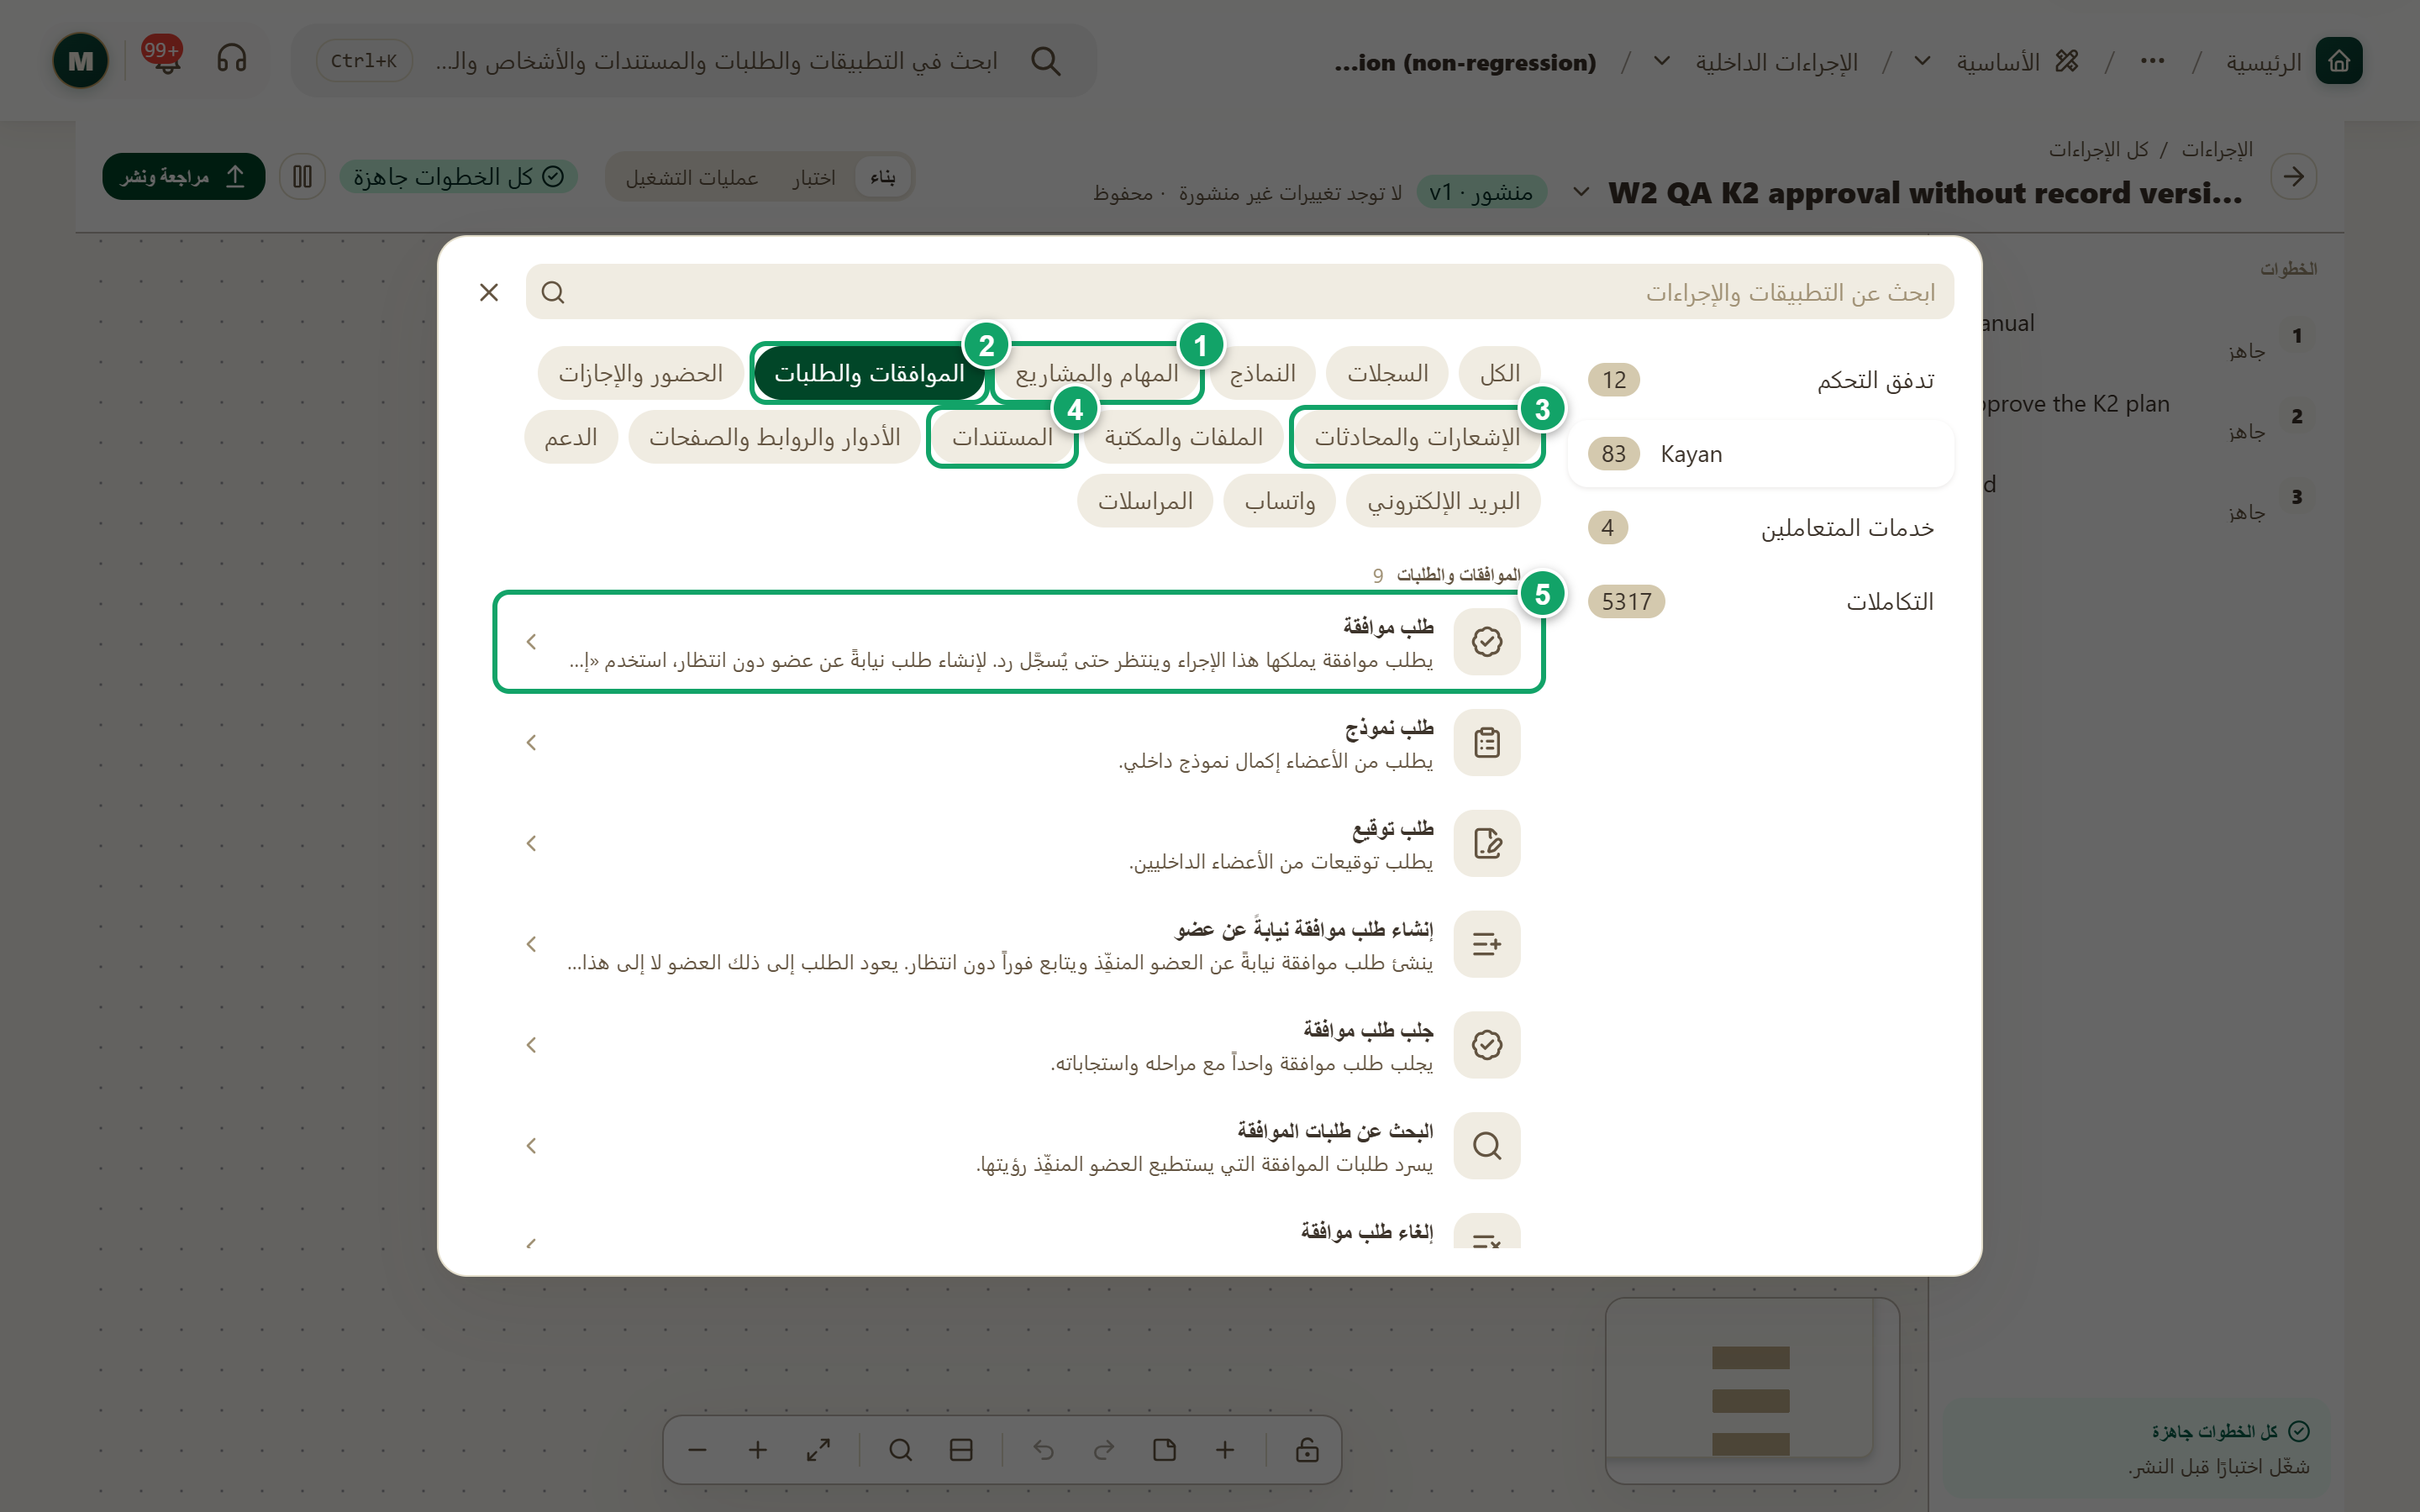
\includegraphics[width=0.95\linewidth,height=0.72\textheight,keepaspectratio]{figures/screens/ch06-isop-people-ar.png}
\caption{قسم «الموافقات والطلبات» في فئة «Kayan»}
\label{fig:builder-isop-people-screen}
\shotnote{تعرض الصورة قائمة الخطوات بعد اختيار قسم «الموافقات والطلبات»، وفيه خطوات طلب الموافقة والنموذج والتوقيع وما يتصل بها. ومن أزرار الأقسام نفسها تصل إلى خطوات المهام والإشعارات والمستندات التي تشرحها هذه الصفحة. ① «المهام والمشاريع»: خطوات إنشاء المهام وتحديثها. ② «الموافقات والطلبات»: القسم المعروض في الصورة. ③ «الإشعارات والمحادثات»: خطوات إرسال الإشعارات. ④ «المستندات»: توليد مستند أو جدول بيانات. ⑤ «طلب موافقة»: الخطوة التي تطلب الموافقة وتنتظر الرد.}
\end{figure}

\begin{table}[H]
\centering
\caption{أهم الخطوات وحقولها}
\label{tab:builder-isop-people-steps}
\begin{tabularx}{\linewidth}{R{3.6cm} Y}
\rcHeaderRow
\thh{الخطوة} & \thh{ما تفعله وأهم حقولها}\\
إنشاء مهمة & تُنشئ مهمة داخلية: «عنوان المهمة» و«تفاصيل المهمة» و«المكلّفون» و«الأولوية» و«تاريخ الاستحقاق»، ويمكن تحديد «نوع المهمة» و«مالك المهمة».\\
طلب موافقة & يطلب موافقة وينتظر الرد: «عنوان الموافقة» و«مراحل الموافقة» بمعتمد واحد على الأقل في كل مرحلة، و«إجراءات الطلب»، و«انتظار الاكتمال» مع «المهلة الزمنية» التي تبدأ بثلاثين يوماً.\\
طلب توقيع & يطلب توقيعات الأعضاء وفق «قواعد التوقيع»، مع تعليمات ومرفقات من المكتبة.\\
إرسال إشعار & يرسل إشعاراً إلى «المستلمون» أو إلى «محدِّدات الأعضاء» مثل الأدوار والأقسام، مع «عنوان الرسالة» و«محتوى الرسالة» ورابط اختياري.\\
خطوات المهام الأخرى & «تحديث مهمة» و«تنفيذ إجراء على مهمة» و«انتظار إجراء على مهمة» و«إضافة تعليق على مهمة».\\
خطوات الموافقات الأخرى & «إرسال تذكير بالموافقة» و«إلغاء طلب موافقة» و«إنشاء طلب موافقة نيابةً عن عضو» الذي لا ينتظر الرد.\\
المستندات & «إنشاء مستند من قالب» و«إنشاء جدول بيانات».\\
\end{tabularx}
\end{table}

\subsection{إجراءات الطلب}

تأتي خطوة «طلب موافقة» بإجراءين جاهزين: الموافقة، وتطلب توقيعاً ويكون التعليق فيها اختيارياً؛ وطلب التغييرات، ويكون التعليق فيها إلزامياً وتنهي الطلب. ولكل إجراء نتيجة تحفظها الخطوة، فتستطيع أن تقرأها في «تفرّع شرطي» بعدها لتختار المسار.

\begin{figure}[H]
\centering
\begin{tikzpicture}[node distance=0.5cm]
\node[stepBox] (a) {\RL{طلب موافقة}};
\node[stepBox,below=of a] (b) {\RL{بانتظار رد المعتمد}};
\node[stepBox,below=of b] (c) {\RL{تفرّع حسب النتيجة}};
\node[stepBox,below=of c] (d) {\RL{إنشاء مهمة}};
\node[stepBox,below=of d] (e) {\RL{إرسال إشعار}};
\draw[flowsTo] (a) -- (b);
\draw[flowsTo] (b) -- (c);
\draw[flowsTo] (c) -- (d);
\draw[flowsTo] (d) -- (e);
\end{tikzpicture}
\rclegend
\caption{مسار يشرك الأشخاص}
\label{fig:builder-isop-people-flow}
\shotnote{يبيّن المخطط أن الموافقة تفصل الإجراء إلى ما قبل الرد وما بعده، فلا تُنشأ المهمة إلا بعد أن يقرر المعتمد. لذلك يأتي القرار بعد طلب الموافقة مباشرة، ليذهب كل رد إلى المسار المناسب له.}
\end{figure}

\subsection{خطوات العمل والتحقق}
\begin{enumerate}
\item أضف «طلب موافقة»، واكتب «عنوان الموافقة»، ثم اضغط «إضافة مرحلة» واختر المعتمدين.
\item راجع «إجراءات الطلب»، وأبقِ «انتظار الاكتمال» مفعّلاً إذا كانت الخطوات التالية تعتمد على الرد.
\item أضف بعده «تفرّع شرطي» يقرأ نتيجة الموافقة.
\item أضف «إنشاء مهمة» في مسار الموافقة، واكتب «عنوان المهمة»، ثم اختر الأعضاء في «المكلّفون».
\end{enumerate}

\textbf{تحقق ومعالجة المشكلة:} يجب ألا تحمل الخطوات شارة «يحتاج إلى تهيئة». فإذا ظهر «مطلوب معتمد واحد على الأقل»، فأضف معتمداً إلى كل مرحلة. وإذا بقي التشغيل منتظراً طويلاً، فأضف بعد الخطوة «إرسال تذكير بالموافقة»، أو قصّر «المهلة الزمنية».

\clearpage
\section{إعداد الخطوة: المدخلات والبيانات والتعبيرات}
\label{sec:builder-feature-isop-inspector}

عندما تضغط خطوة على اللوحة تُفتح لوحة إعدادها بجانب اللوحة الرئيسية. وفيها تعدّل اسم الخطوة، وتملأ مدخلاتها، وتختار مصدر كل قيمة: قيمة تكتبها بنفسك، أو بيانات من المشغّل أو من خطوة سابقة، أو تعبيراً يحسب القيمة. وتُحفظ التغييرات تلقائياً.

\textbf{المسار ومن يستخدمه:} المحرر ← اضغط الخطوة ← لوحة الإعداد. يستخدمها من يبني الإجراء.

\begin{rcnote}[مثال: شركة الأفق]
في خطوة «إنشاء مهمة»، يضغط المسؤول «إدراج بيانات» (②) بجانب «عنوان المهمة»، ويختار رقم الطلب من بيانات المشغّل، فيصبح العنوان «تجهيز الزيارة \en{HZN-VR-0001}» لكل طلب بحسب رقمه.
\end{rcnote}

\begin{figure}[H]
\centering
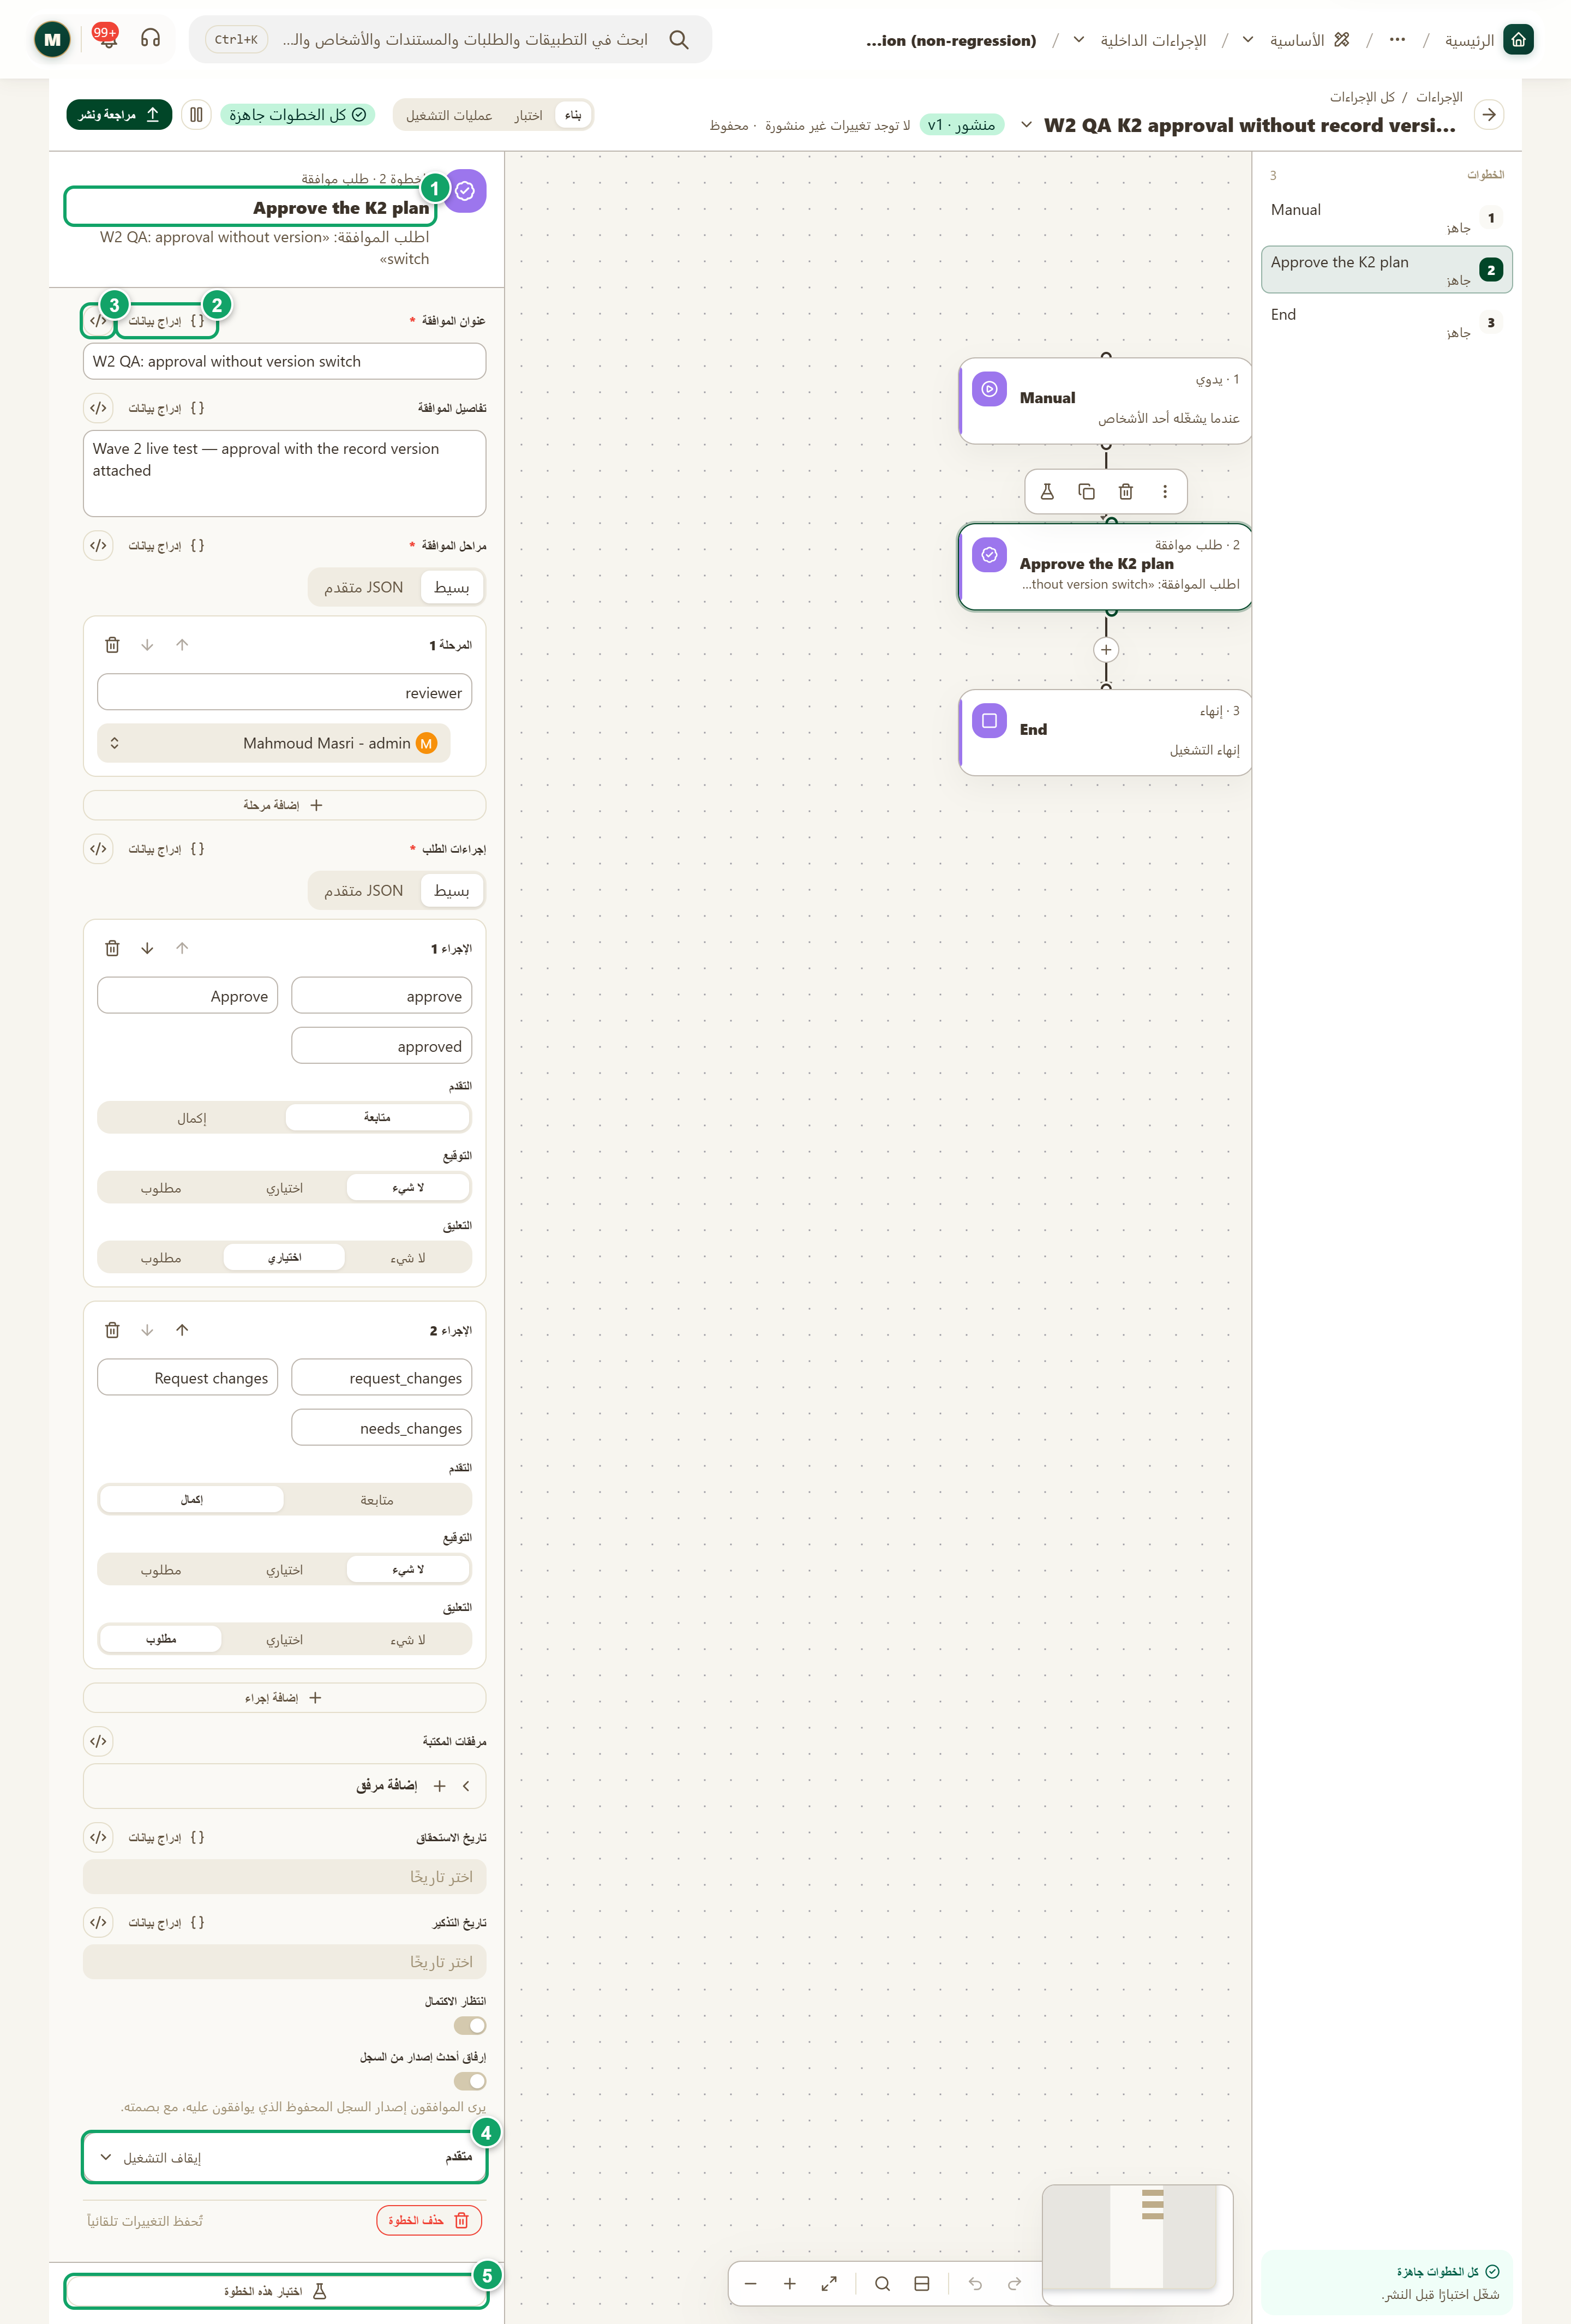
\includegraphics[width=0.95\linewidth,height=0.72\textheight,keepaspectratio]{figures/screens/ch06-isop-inspector-ar.png}
\caption{لوحة إعداد خطوة «طلب موافقة»}
\label{fig:builder-isop-inspector-screen}
\shotnote{تعرض الصورة لوحة إعداد خطوة «طلب موافقة» في الإجراء الاختباري، وفيها حقول الخطوة كاملة من العنوان إلى «متقدم». ويتكرر بجانب كل حقل الزران نفسهما، فتعرف أن أي قيمة يمكن أن تُكتب أو تُدرج أو تُحسب. ① اسم الخطوة: تعدّله بالضغط عليه. ② «إدراج بيانات»: يدرج قيمة من المشغّل أو من خطوة سابقة. ③ زر التعبير: يحوّل الحقل إلى تعبير تكتبه. ④ «متقدم»: الوصف والاسم المرجعي وما يحدث عند الفشل. ⑤ «اختبار هذه الخطوة»: يشغّل الخطوة وحدها.}
\end{figure}

\begin{table}[H]
\centering
\caption{أجزاء لوحة إعداد الخطوة}
\label{tab:builder-isop-inspector-parts}
\begin{tabularx}{\linewidth}{R{3.6cm} Y}
\rcHeaderRow
\thh{الجزء} & \thh{ما يقدمه}\\
الرأس & اسم الخطوة، وتعدّله بالضغط عليه، وتحته رقمها ونوعها مثل «الخطوة 3 · طلب موافقة».\\
المدخلات & حقول الخطوة، والمطلوب منها معلَّم. وتظهر المشكلات تحت الحقل الناقص مباشرة.\\
إدراج بيانات & يفتح قائمة بالبيانات المتاحة للحقل: المشغّل، والخطوات السابقة، والعنصر الحالي داخل «لكل عنصر»، و«المتغيرات». وتظهر بجانب كل حقل قيمة نموذجية من آخر اختبار.\\
زر التعبير & يحوّل الحقل إلى تعبير تكتبه بنفسك عندما تحتاج إلى حساب أو صيغة.\\
متقدم & «إذا فشلت هذه الخطوة» و«تخطي هذه الخطوة» و«الوصف» و«الاسم المرجعي» الذي تستخدمه الصيغ.\\
التذييل & «اختبار هذه الخطوة» و«حذف الخطوة»، مع عبارة «تُحفظ التغييرات تلقائياً».\\
\end{tabularx}
\end{table}

\begin{rcwarn}[الاسم المرجعي]
تشير الصيغ إلى الخطوة باسمها المرجعي، لذلك اجعله مقروءاً بأحرف إنجليزية صغيرة وأرقام وشرطات سفلية. وعند تغييره يحدّث النظام كل صيغة تشير إلى الخطوة، لكنه يرفض اسماً تستخدمه خطوة أخرى.
\end{rcwarn}

\begin{figure}[H]
\centering
\begin{tikzpicture}[node distance=0.5cm]
\node[stepBox] (a) {\RL{اختيار الخطوة}};
\node[stepBox,below=of a] (b) {\RL{تعبئة المدخلات}};
\node[stepBox,below=of b] (c) {\RL{إدراج بيانات سابقة}};
\node[stepBox,below=of c] (d) {\RL{كتابة تعبير عند الحاجة}};
\node[stepBox,below=of d] (e) {\RL{اختبار هذه الخطوة}};
\draw[flowsTo] (a) -- (b);
\draw[flowsTo] (b) -- (c);
\draw[flowsTo] (c) -- (d);
\draw[flowsTo] (d) -- (e);
\end{tikzpicture}
\rclegend
\caption{من الحقل الفارغ إلى قيمة صحيحة}
\label{fig:builder-isop-inspector-flow}
\shotnote{يرتب المخطط مصادر القيمة من الأبسط إلى الأعقد: تكتب القيمة، فإن كانت تتغير مع كل تشغيل أدرجتها من بيانات سابقة، وتلجأ إلى التعبير عند الحاجة إلى حساب. ويختم باختبار الخطوة لترى القيمة الفعلية التي استلمتها.}
\end{figure}

\subsection{خطوات العمل والتحقق}
\begin{enumerate}
\item اضغط الخطوة على اللوحة أو في قائمة «الخطوات».
\item املأ الحقول المطلوبة، واضغط «إدراج بيانات» بجانب أي حقل تأتي قيمته من المشغّل أو من خطوة سابقة.
\item ابحث في «ابحث في الحقول» عن الحقل الذي تريده، ثم اضغطه ليُدرج في مكانه.
\item افتح «متقدم» إذا أردت كتابة وصف للخطوة أو تعديل اسمها المرجعي.
\end{enumerate}

\textbf{تحقق ومعالجة المشكلة:} يجب أن تظهر البيانات المدرجة داخل الحقل مرجعاً مميزاً، وأن تختفي شارة «يحتاج إلى تهيئة». فإذا ظهر في قائمة البيانات «شغّل اختبارًا لرؤية قيم نموذجية هنا»، فشغّل اختباراً أولاً لترى القيم. وإذا نبّهك المحرر إلى مرجع بيانات غير مكتمل في حقل، فاحذف المرجع وأدرجه من جديد.

\clearpage
\section{معالجة الأخطاء وتخطي الخطوات}
\label{sec:builder-feature-isop-errors}

قد تفشل خطوة لأن خدمة خارجية لم تستجب، أو لأن سجلاً لم يعد موجوداً. ويحدد قسم «معالجة الأخطاء» ما يحدث عندئذ: أن يتوقف التشغيل كله، أو أن يتابع في مسار بديل تبنيه أنت. وتستطيع أيضاً أن تطلب إعادة المحاولة قبل اعتبار الخطوة فاشلة، أو أن تُبقي الخطوة في المسار دون تشغيلها مؤقتاً.

\textbf{المسار ومن يستخدمه:} المحرر ← اضغط الخطوة ← «متقدم» ← «إذا فشلت هذه الخطوة». يستخدمه من يبني الإجراء. ولا يظهر الخياران لخطوات المشغّل و«تفرّع شرطي» و«إنهاء».

\begin{rcnote}[مثال: شركة الأفق]
يفعّل المسؤول «إعادة المحاولة قبل الاستسلام» في خطوة «إرسال إشعار» إلى عمر حداد، ويختار «اتباع مسار الفشل» (③) ليرسل في مسار الفشل إشعاراً بديلاً إلى سارة الخطيب.
\end{rcnote}

\begin{figure}[H]
\centering
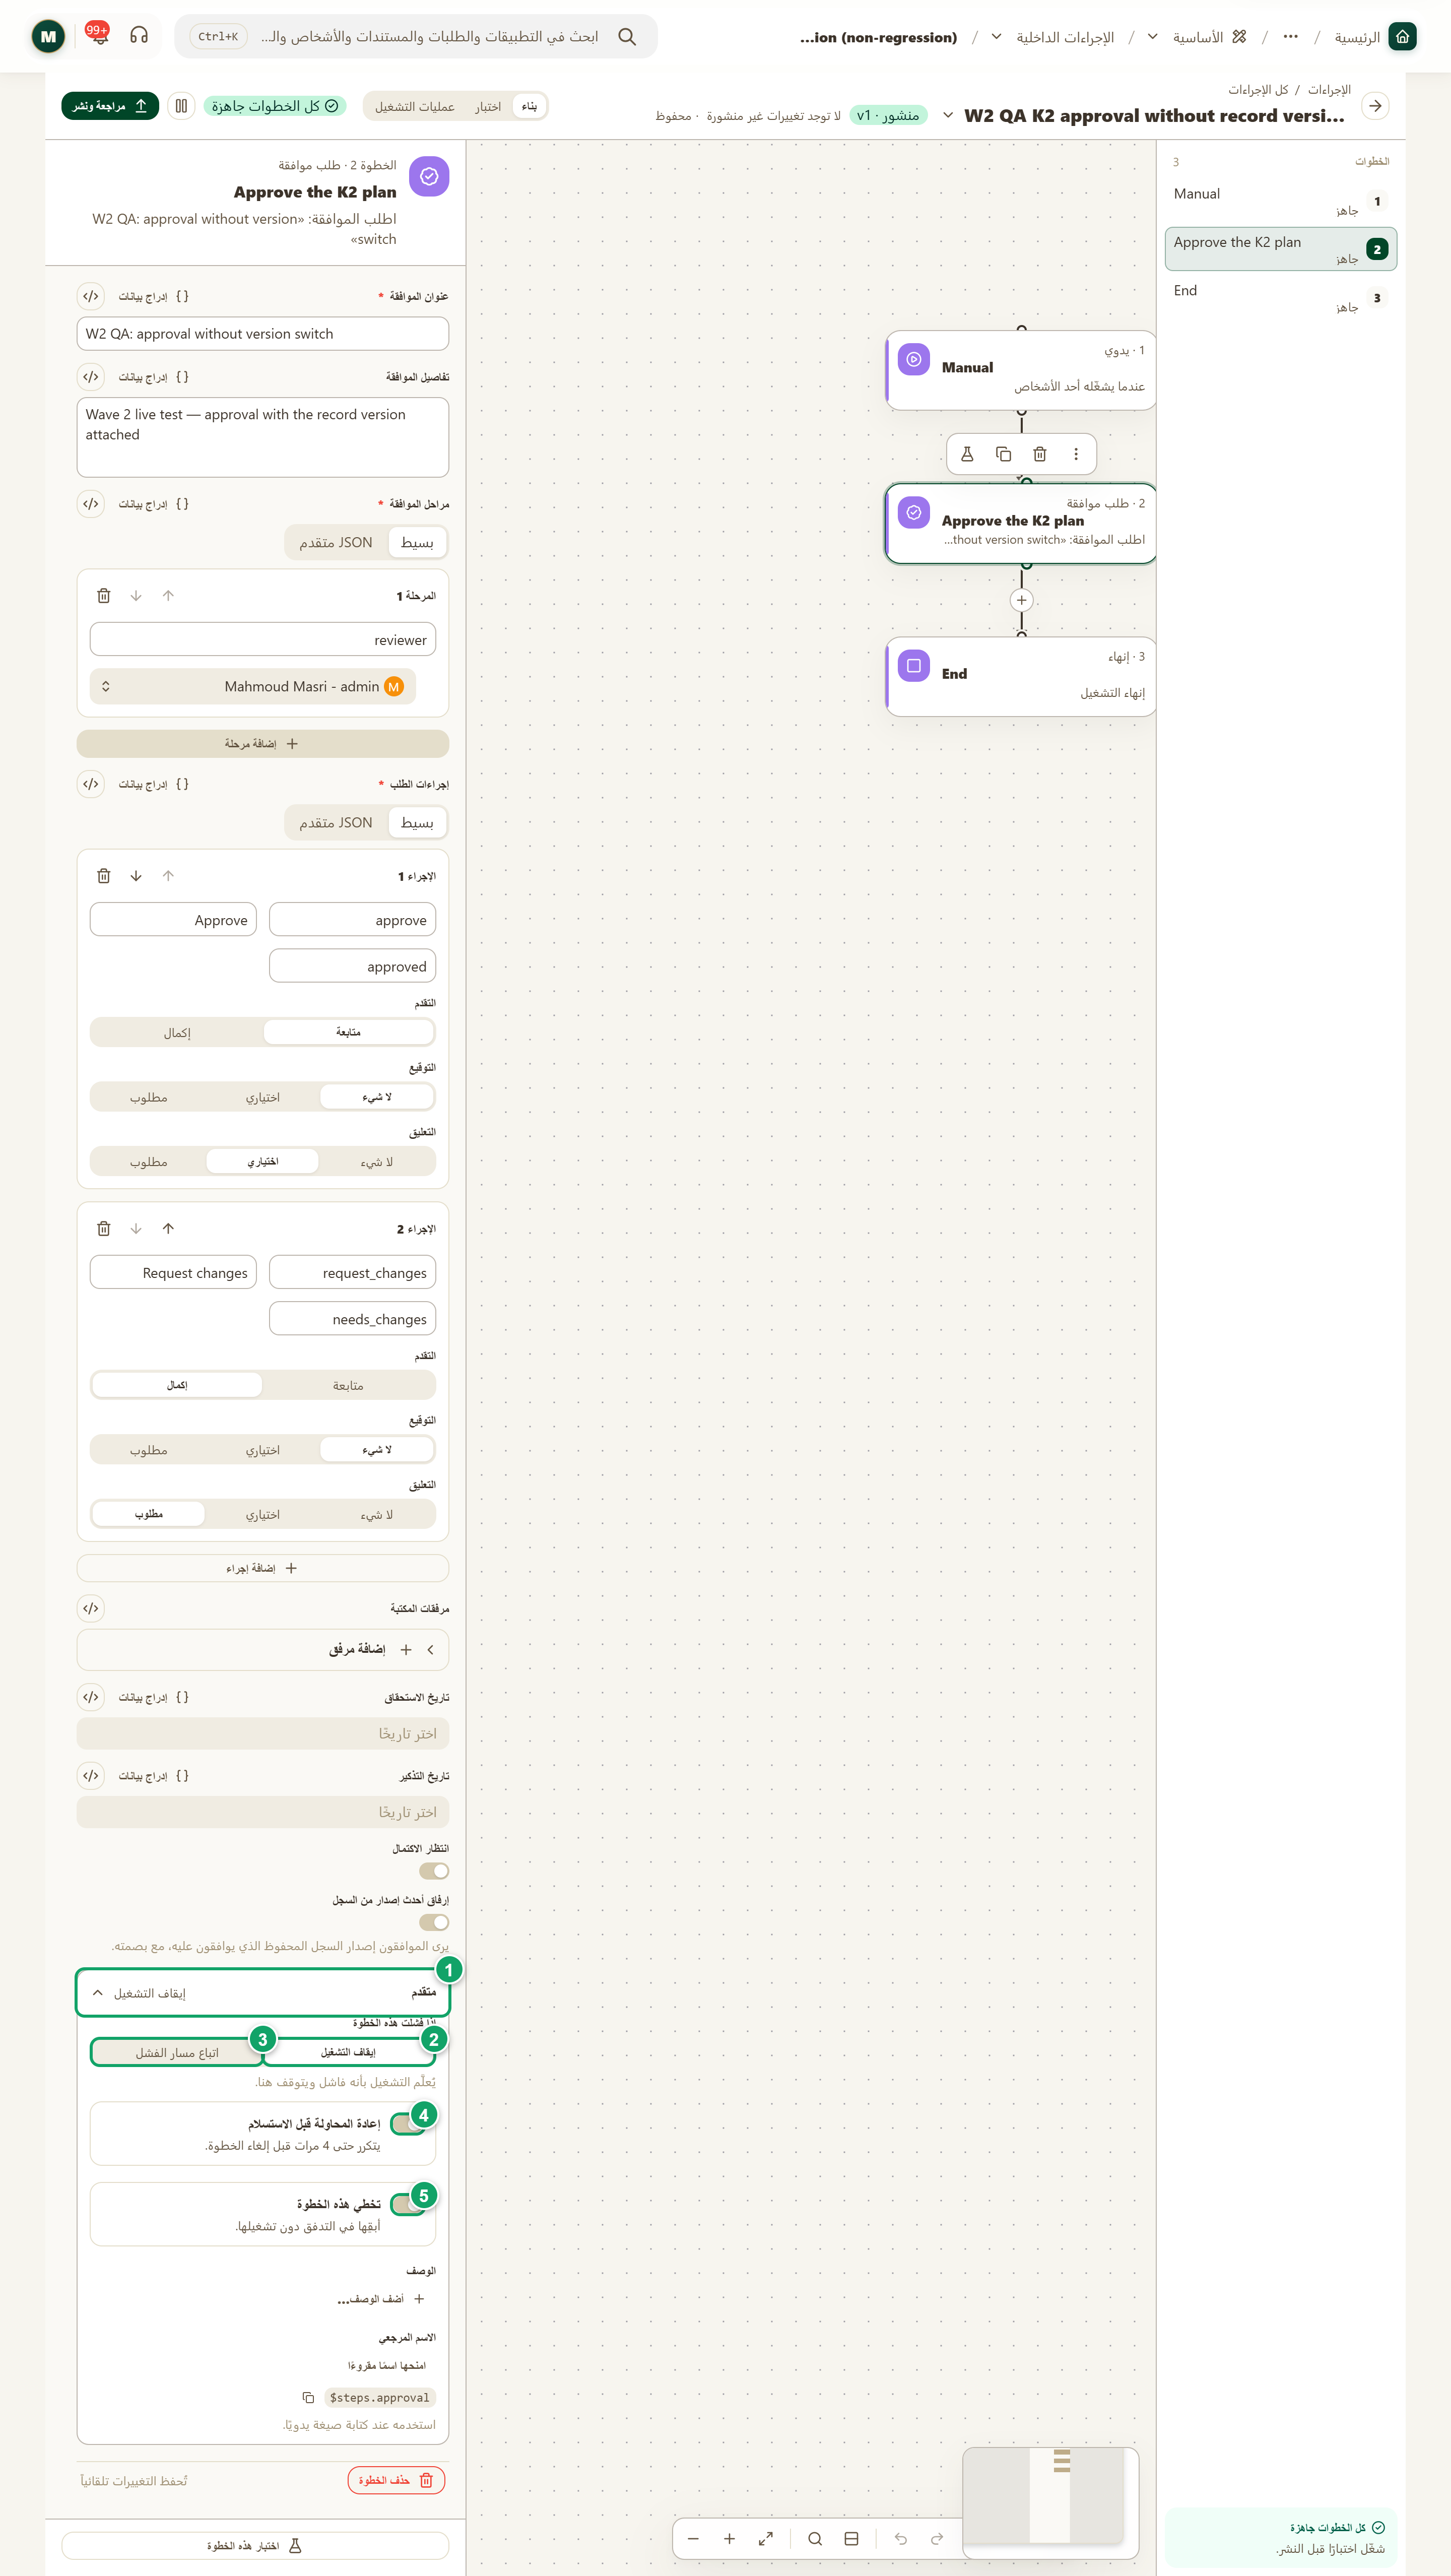
\includegraphics[width=0.95\linewidth,height=0.72\textheight,keepaspectratio]{figures/screens/ch06-isop-errors-ar.png}
\caption{خيارات الفشل والتخطي في «متقدم»}
\label{fig:builder-isop-errors-screen}
\shotnote{تعرض الصورة قسم «متقدم» مفتوحاً في خطوة «طلب موافقة»، والاختيار فيه على الوضع الافتراضي «إيقاف التشغيل» مع إيقاف المفتاحين. ويُلخَّص الاختيار بجانب عنوان «متقدم»، فتعرف سلوك الخطوة عند الفشل دون أن تفتح القسم. ① «متقدم»: يفتح الخيارات. ② «إيقاف التشغيل»: يتوقف التشغيل عند هذه الخطوة. ③ «اتباع مسار الفشل»: يضيف مساري نجاح وفشل. ④ «إعادة المحاولة قبل الاستسلام»: حتى أربع محاولات. ⑤ «تخطي هذه الخطوة»: تبقى الخطوة دون أن تعمل.}
\end{figure}

\begin{table}[H]
\centering
\caption{خيارات الفشل والتخطي}
\label{tab:builder-isop-errors-options}
\begin{tabularx}{\linewidth}{R{3.6cm} Y}
\rcHeaderRow
\thh{الخيار} & \thh{ما يحدث}\\
إيقاف التشغيل & هو الخيار الافتراضي: يُعلَّم التشغيل بأنه فاشل ويتوقف عند هذه الخطوة.\\
اتباع مسار الفشل & يضيف بعد الخطوة مسارين، نجاح وفشل، فيتابع التشغيل في مسار الفشل عند الخطأ بدلاً من التوقف. وعند إلغائه يبقى مسار النجاح وحده.\\
إعادة المحاولة قبل الاستسلام & يعيد تنفيذ الخطوة حتى أربع مرات قبل اعتبارها فاشلة.\\
تخطي هذه الخطوة & يُبقي الخطوة في المسار دون تشغيلها، وتظهر على اللوحة بشارة «تم التخطي». ولا يتوفر لخطوات التحكم مثل «تفرّع شرطي» و«لكل عنصر» و«إنهاء».\\
\end{tabularx}
\end{table}

\begin{figure}[H]
\centering
\begin{tikzpicture}[node distance=0.5cm]
\node[stepBox] (a) {\RL{تنفيذ الخطوة}};
\node[stepBox,below=of a] (b) {\RL{خطأ أثناء التنفيذ}};
\node[stepBox,below=of b] (c) {\RL{إعادة المحاولة إن فُعّلت}};
\node[stepBox,below=of c] (d) {\RL{إيقاف أو مسار الفشل}};
\node[stepBox,below=of d] (e) {\RL{مراجعة التشغيل}};
\draw[flowsTo] (a) -- (b);
\draw[flowsTo] (b) -- (c);
\draw[flowsTo] (c) -- (d);
\draw[flowsTo] (d) -- (e);
\end{tikzpicture}
\rclegend
\caption{ما يحدث عند فشل خطوة}
\label{fig:builder-isop-errors-flow}
\shotnote{يبيّن المخطط أن إعادة المحاولة تأتي أولاً، ولا يُطبَّق اختيار الإيقاف أو مسار الفشل إلا بعد أن تستنفد المحاولات. وفي الحالتين يبقى الخطأ مسجلاً في عملية التشغيل، فتراجعه لتعرف سببه.}
\end{figure}

\subsection{خطوات العمل والتحقق}
\begin{enumerate}
\item اضغط الخطوة، ثم افتح «متقدم».
\item في «إذا فشلت هذه الخطوة»، اختر «إيقاف التشغيل» أو «اتباع مسار الفشل».
\item إذا اخترت مسار الفشل، فأضف على مسار الفشل في اللوحة الخطوات التي تعالج الخطأ.
\item فعّل «إعادة المحاولة قبل الاستسلام» للخطوات التي تتصل بخدمات قد تتأخر.
\end{enumerate}

\textbf{تحقق ومعالجة المشكلة:} عند اختيار مسار الفشل يجب أن ترى خطين يخرجان من الخطوة، وأن يُلخَّص الاختيار بجانب «متقدم». وإذا نسيت خطوة على «تخطي هذه الخطوة» فلن تعمل في أي تشغيل، فابحث في اللوحة عن شارة «تم التخطي» قبل النشر.

\clearpage
\section{الاتصالات والمتغيرات}
\label{sec:builder-feature-isop-connections}

بعض الخطوات تتصل بخدمات خارج \en{KayanOS}، فتحتاج إلى حساب في تلك الخدمة. وتحفظ هذه الحسابات في تبويب «الاتصالات»، فتختار الخطوة الاتصال بدلاً من أن تحمل كلمة مرور. أما «المتغيرات» فقيم مشفرة تخص المؤسسة، مثل رمز وصول أو رقم ثابت، تستخدمها في تعبيرات أي إجراء دون أن تكتبها في كل خطوة.

\textbf{المسار ومن يستخدمه:} «الإجراءات الداخلية» ← «الاتصالات» أو «المتغيرات»، أو حقل «الاتصال» داخل خطوة من «التكاملات». يستخدمها من يبني الإجراءات ويدير حسابات المؤسسة.

\begin{rcnote}[مثال: شركة الأفق]
يضيف المسؤول متغيراً اسمه \en{HZN\_ALEPPO\_EMAIL} يحمل بريد فرع حلب، ثم يستخدمه في التعبيرات بدلاً من كتابة العنوان في كل خطوة. وعندما يتغير البريد، يغيّر قيمة المتغير مرة واحدة.
\end{rcnote}

\begin{figure}[H]
\centering
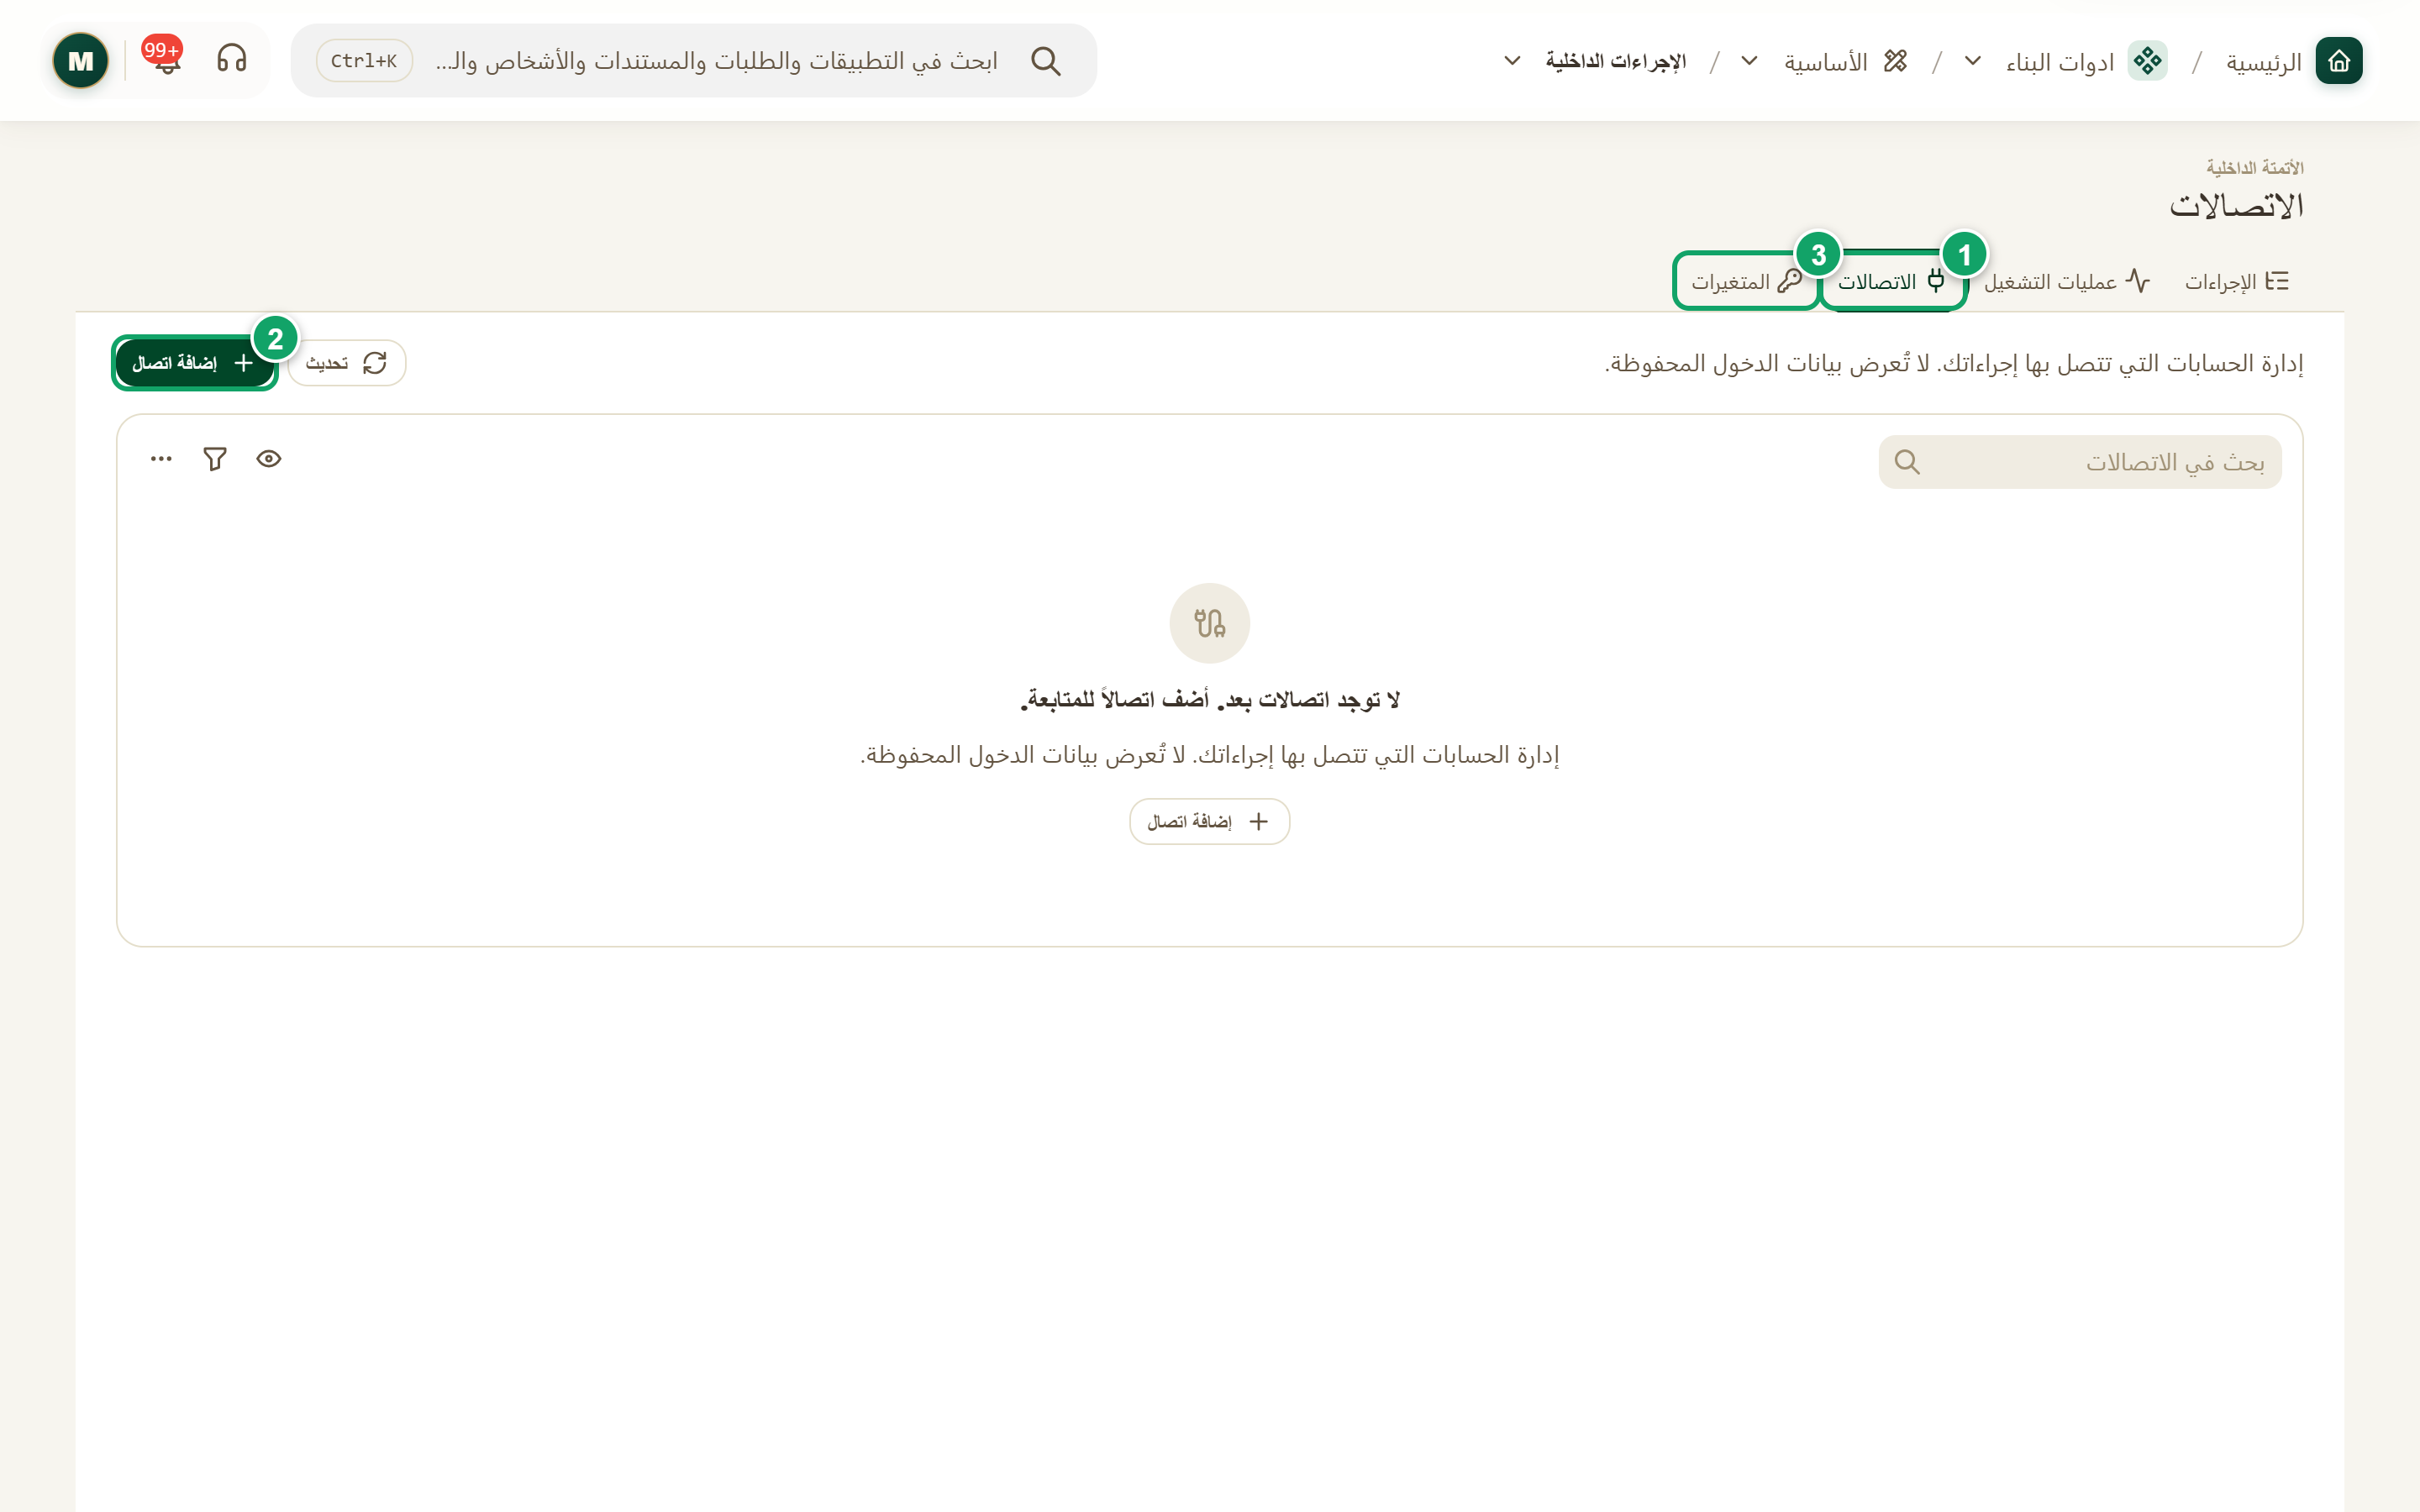
\includegraphics[width=0.95\linewidth,height=0.72\textheight,keepaspectratio]{figures/screens/ch06-isop-connections-ar.png}
\caption{تبويب «الاتصالات» في الإجراءات الداخلية}
\label{fig:builder-isop-connections-screen}
\shotnote{تعرض الصورة تبويب «الاتصالات» في مؤسسة الاختبار، وهو فارغ لأن أحداً لم يضف حساباً خارجياً بعد. وتوضح العبارة أعلى القائمة أن بيانات الدخول المحفوظة لا تُعرض أبداً، لذلك تختار الخطوة الاتصال باسمه فقط. ① «الاتصالات»: التبويب الذي يحفظ حسابات الخدمات الخارجية. ② «إضافة اتصال»: يبدأ ربط حساب جديد. ③ «المتغيرات»: التبويب المجاور للقيم المشفّرة التي تستخدمها التعبيرات.}
\end{figure}

\begin{table}[H]
\centering
\caption{إدارة الاتصالات}
\label{tab:builder-isop-connections-parts}
\begin{tabularx}{\linewidth}{R{3.6cm} Y}
\rcHeaderRow
\thh{الأداة} & \thh{ما تفعله}\\
إضافة اتصال & تختار «التطبيق» ثم «طريقة الاتصال»: «تسجيل الدخول إلى حساب» في نافذة جديدة، أو إدخال «مفتاح API أو رمز الوصول». ثم تكتب «اسم الاتصال» وتضغط «حفظ الاتصال».\\
الحالة & «نشط»، أو «يلزم إعادة الاتصال» عندما تنتهي صلاحية الدخول.\\
اختبار & يتحقق من الاتصال ويعرض «نجح اختبار الاتصال» أو «فشل اختبار الاتصال».\\
تحديث الاتصال & يعيد تسجيل الدخول أو يستبدل بيانات الدخول، دون أن يغيّر الخطوات التي تستخدمه.\\
إعادة تسمية، حذف & عند الحذف تحتاج الخطوات التي تستخدم الاتصال إلى بديل.\\
\end{tabularx}
\end{table}

\begin{table}[H]
\centering
\caption{إدارة المتغيرات}
\label{tab:builder-isop-connections-variables}
\begin{tabularx}{\linewidth}{R{3.6cm} Y}
\rcHeaderRow
\thh{الأداة} & \thh{ما تفعله}\\
متغير جديد & تكتب «الاسم» بأحرف وأرقام وشرطة سفلية فقط، ثم «القيمة»، ثم تضغط «إنشاء متغير». ولا تظهر القيمة مرة أخرى بعد حفظها.\\
نسخ المرجع & ينسخ صيغة الإشارة إلى المتغير لتلصقها في تعبير.\\
تغيير القيمة & يستبدل القيمة المحفوظة بقيمة جديدة.\\
حذف المتغير & يحذف المتغير، فتفشل التعبيرات التي تستخدمه.\\
\end{tabularx}
\end{table}

\begin{figure}[H]
\centering
\begin{tikzpicture}[node distance=0.5cm]
\node[stepBox] (a) {\RL{إضافة اتصال أو متغير}};
\node[stepBox,below=of a] (b) {\RL{اختباره أو نسخ مرجعه}};
\node[stepBox,below=of b] (c) {\RL{اختياره في الخطوة}};
\node[stepBox,below=of c] (d) {\RL{تحديثه عند التغيير}};
\draw[flowsTo] (a) -- (b);
\draw[flowsTo] (b) -- (c);
\draw[flowsTo] (c) -- (d);
\end{tikzpicture}
\rclegend
\caption{دورة حياة الاتصال والمتغير}
\label{fig:builder-isop-connections-flow}
\shotnote{يوضح المخطط أن الاتصال أو المتغير يُنشأ مرة واحدة ثم تستخدمه خطوات كثيرة. لذلك يكفي تحديثه في مكانه عند تغيّر كلمة المرور أو القيمة، دون فتح كل إجراء يعتمد عليه.}
\end{figure}

\subsection{خطوات العمل والتحقق}
\begin{enumerate}
\item افتح تبويب «الاتصالات»، واضغط «إضافة اتصال»، واختر «التطبيق».
\item اختر «طريقة الاتصال»، وسجّل الدخول أو أدخل المفتاح، ثم اكتب «اسم الاتصال» واضغط «حفظ الاتصال».
\item اضغط «اختبار» بجانب الاتصال، ثم اختره في حقل «الاتصال» داخل الخطوة.
\item لإضافة متغير، افتح «المتغيرات» واضغط «متغير جديد»، ثم اضغط «نسخ المرجع» لتستخدمه في تعبير.
\end{enumerate}

\textbf{تحقق ومعالجة المشكلة:} يجب أن يظهر الاتصال بحالة «نشط». فإذا ظهر «اسمح بالنوافذ المنبثقة لربط هذا الحساب»، فاسمح بالنوافذ المنبثقة للموقع ثم أعد المحاولة. وإذا أصبحت الحالة «يلزم إعادة الاتصال»، فاضغط «تحديث الاتصال» وسجّل الدخول من جديد.

\clearpage
\section{اختبار الإجراء}
\label{sec:builder-feature-isop-testing}

يجرّب الاختبار المسودة قبل نشرها، فترى نتيجة كل خطوة على اللوحة. ويوفر وضع «اختبار» طريقتين: «محاكاة (آمنة)» تشغّل المسودة دون إنشاء سجلات أو إرسال أي شيء، و«تشغيل فعلي» يشغّل الإصدار المنشور بآثار حقيقية. وتستطيع كذلك أن تختبر خطوة واحدة دون تشغيل المسار كله.

\textbf{المسار ومن يستخدمه:} المحرر ← «اختبار» ← لوحة «اختبار هذه المسودة»، أو لوحة الخطوة ← «اختبار هذه الخطوة». يستخدمه من يبني الإجراء قبل كل نشر.

\begin{rcnote}[مثال: شركة الأفق]
يكتب المسؤول في «بيانات الاختبار» طلب زيارة لفرع حلب، ثم يشغّل «محاكاة (آمنة)» (③). فيرى أن المسار وصل إلى «طلب موافقة» دون أن يصل أي طلب حقيقي إلى سارة الخطيب.
\end{rcnote}

\begin{figure}[H]
\centering
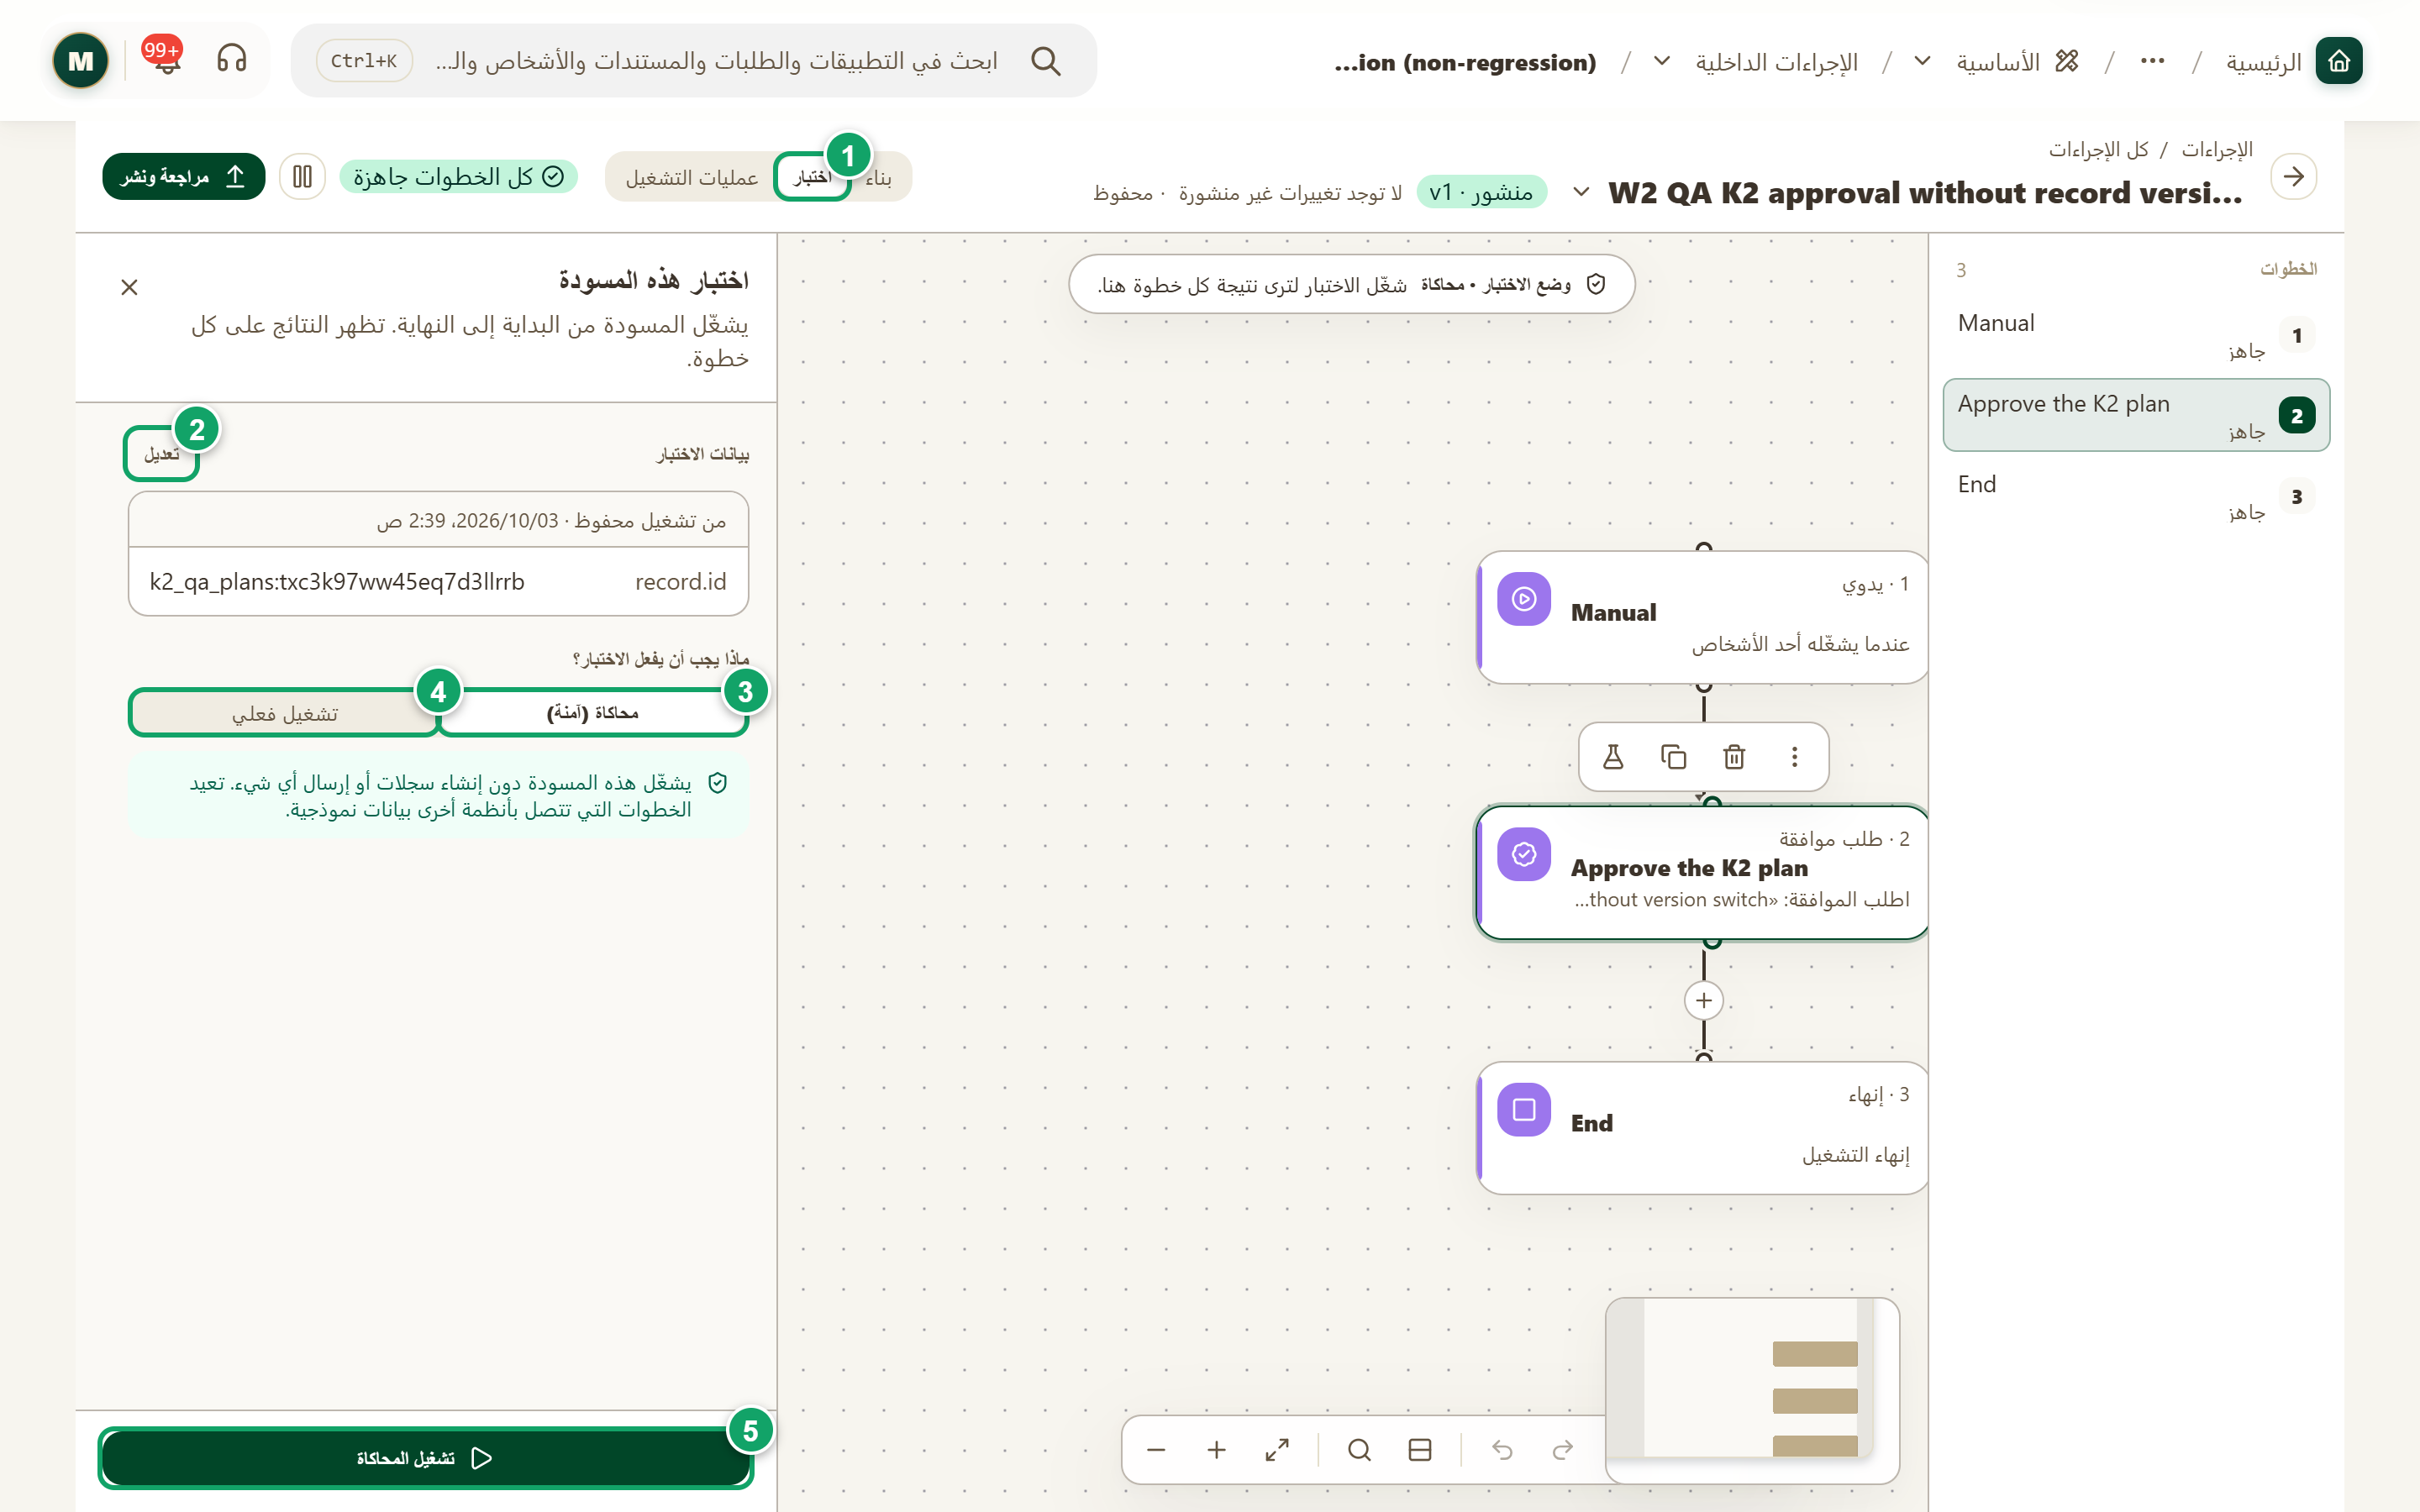
\includegraphics[width=0.95\linewidth,height=0.72\textheight,keepaspectratio]{figures/screens/ch06-isop-testing-ar.png}
\caption{لوحة «اختبار هذه المسودة» في وضع «اختبار»}
\label{fig:builder-isop-testing-screen}
\shotnote{تعرض الصورة الإجراء الاختباري في وضع «اختبار»، وبيانات الاختبار مأخوذة من تشغيل محفوظ، والاختيار على «محاكاة (آمنة)». ولم يُشغَّل أي اختبار عند الالتقاط، فاللوحة تبيّن ما تختاره قبل التشغيل لا نتيجته. ① «اختبار»: الوضع الذي تجرّب فيه المسودة. ② «تعديل»: يغيّر بيانات الاختبار. ③ «محاكاة (آمنة)»: تجربة بلا أثر حقيقي. ④ «تشغيل فعلي»: تشغيل للإصدار المنشور بآثار حقيقية. ⑤ «تشغيل المحاكاة»: يبدأ التجربة.}
\end{figure}

\begin{table}[H]
\centering
\caption{أجزاء لوحة الاختبار}
\label{tab:builder-isop-testing-panel}
\begin{tabularx}{\linewidth}{R{3.6cm} Y}
\rcHeaderRow
\thh{الجزء} & \thh{ما يقدمه}\\
بيانات الاختبار & البيانات التي يبدأ بها المشغّل. تعدّلها بـ«تعديل»، أو تختار «استخدام بيانات آخر تشغيل». ويجب أن تكون كائن \en{JSON}.\\
ماذا يجب أن يفعل الاختبار؟ & «محاكاة (آمنة)»: تشغّل المسودة، وتعيد الخطوات المتصلة بأنظمة أخرى بيانات نموذجية. «تشغيل فعلي»: يشغّل الإصدار المنشور، فتُنشأ السجلات وتُرسل الرسائل.\\
الموافقة على التشغيل الفعلي & مربع تؤكد فيه أن التشغيل قد يُحدث آثاراً فعلية وقد ينتظر استجابات خارجية. ولا يعمل الزر قبل تأكيده.\\
أحدث اختبار & «نجح الاختبار» أو «فشل الاختبار عند» خطوة محددة أو «الاختبار بانتظار رد»، مع عدد الخطوات والمدة و«السجلات والتفاصيل».\\
اختبار هذه الخطوة فقط & يشغّل الخطوة المختارة وحدها ببيانات اختبار محفوظة. ولخطوات \en{Kayan} ينفّذ إجراءً حقيقياً، فيطلب موافقتك قبل التشغيل.\\
\end{tabularx}
\end{table}

\begin{figure}[H]
\centering
\begin{tikzpicture}[node distance=0.5cm]
\node[stepBox] (a) {\RL{تجهيز بيانات الاختبار}};
\node[stepBox,below=of a] (b) {\RL{محاكاة آمنة للمسودة}};
\node[stepBox,below=of b] (c) {\RL{قراءة النتيجة على الخطوات}};
\node[stepBox,below=of c] (d) {\RL{إصلاح الخطوة وإعادة الاختبار}};
\node[stepBox,below=of d] (e) {\RL{تشغيل فعلي بعد النشر}};
\draw[flowsTo] (a) -- (b);
\draw[flowsTo] (b) -- (c);
\draw[flowsTo] (c) -- (d);
\draw[flowsTo] (d) -- (e);
\end{tikzpicture}
\rclegend
\caption{من المحاكاة إلى التشغيل الفعلي}
\label{fig:builder-isop-testing-flow}
\shotnote{يضع المخطط المحاكاة قبل كل شيء لأنها تختبر المسودة نفسها دون أي أثر على البيانات أو الأشخاص. أما التشغيل الفعلي فيأتي أخيراً، لأنه لا يعمل إلا على الإصدار المنشور وقد يُنشئ سجلات ويرسل طلبات حقيقية.}
\end{figure}

\subsection{خطوات العمل والتحقق}
\begin{enumerate}
\item اضغط «اختبار» في رأس المحرر، ثم اضغط «تعديل» في «بيانات الاختبار» واكتب القيم التي تريد تجربتها، واضغط «تم».
\item اختر «محاكاة (آمنة)»، ثم اضغط «تشغيل المحاكاة».
\item اقرأ النتيجة على كل خطوة، واضغط الخطوة الفاشلة لترى ما استلمته وما أعادته.
\item أصلح الخطوة في وضع «بناء»، ثم ارجع واضغط «تشغيل الاختبار مجددًا».
\item بعد النشر، إذا أردت تجربة فعلية، فاختر «تشغيل فعلي» وأكّد الموافقة، ثم اضغط زر التشغيل الفعلي.
\end{enumerate}

\textbf{تحقق ومعالجة المشكلة:} يجب أن يظهر «نجح الاختبار» في «أحدث اختبار». فإذا ظهر «خطوات ما زالت تحتاج إلى تهيئة»، فأكمل تلك الخطوات أولاً لأن الاختبار قد يتوقف عندها. وإذا لم يعمل «تشغيل فعلي»، فانشر الإجراء أولاً، وتأكد أن الخادم «متصل».

\clearpage
\section{عمليات التشغيل وسجلها}
\label{sec:builder-feature-isop-runs}

عملية التشغيل هي مرة واحدة عمل فيها الإجراء من المشغّل حتى النهاية أو حتى توقف. ويحفظ النظام لكل عملية حالتها ونتيجة كل خطوة فيها، فتعرف أين نجح الإجراء وأين فشل أو ينتظر. وتراجع العمليات من مكانين: وضع «عمليات التشغيل» في المحرر لإجراء واحد على لوحته، وتبويب «عمليات التشغيل» في الصفحة الرئيسية لكل الإجراءات معاً.

\textbf{المسار ومن يستخدمه:} المحرر ← «عمليات التشغيل»، أو «الإجراءات الداخلية» ← «عمليات التشغيل». يستخدمه من يبني الإجراء ومن يتابع تشغيله.

\begin{rcnote}[مثال: شركة الأفق]
يفتح المسؤول تشغيل الطلب \en{HZN-VR-0001} فيجده «بانتظار استجابة» عند «طلب موافقة»، مع مدة الانتظار ورابط يفتح الطلب. وبعد أن توافق سارة الخطيب يكتمل التشغيل وتظهر مهمة عمر حداد.
\end{rcnote}

\begin{figure}[H]
\centering
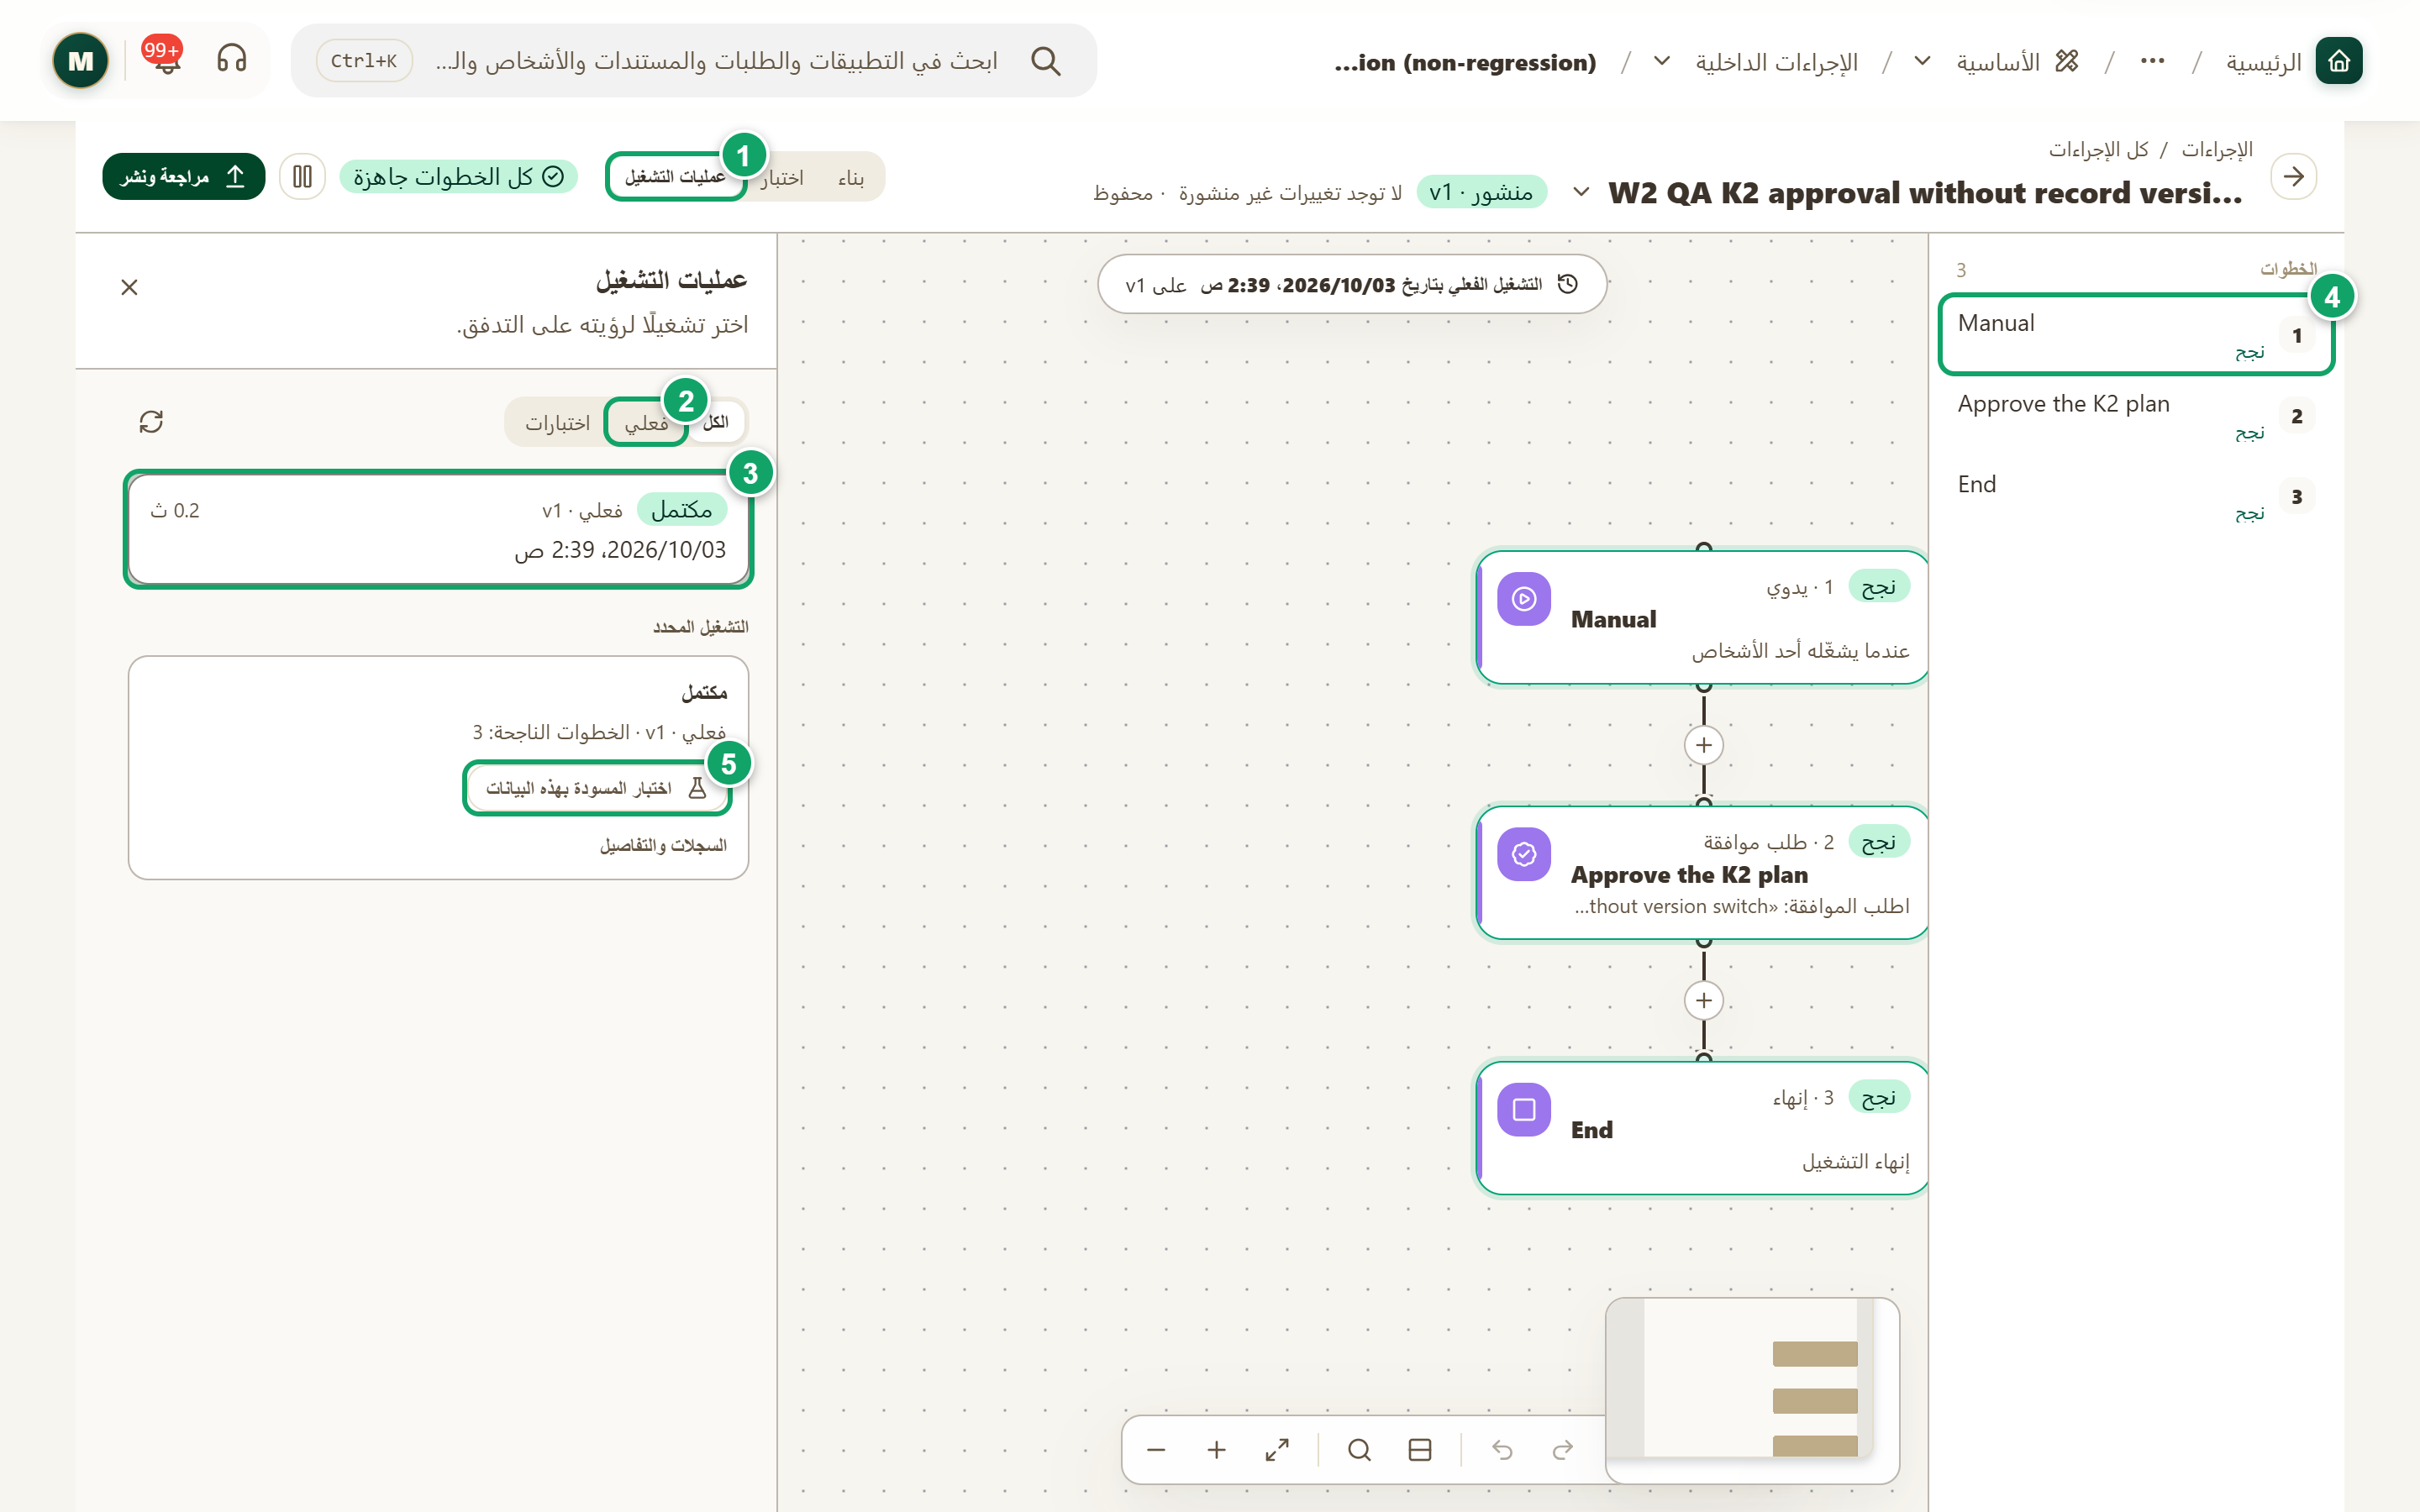
\includegraphics[width=0.95\linewidth,height=0.72\textheight,keepaspectratio]{figures/screens/ch06-isop-runs-ar.png}
\caption{تشغيل مكتمل معروض في وضع «عمليات التشغيل»}
\label{fig:builder-isop-runs-screen}
\shotnote{تعرض الصورة التشغيل الوحيد للإجراء الاختباري بعد اختياره، وقد ظهرت نتيجة كل خطوة على اللوحة وفي قائمة الخطوات. وبهذا ترى أين نجح التشغيل أو توقف دون أن تقرأ السجلات التقنية. ① «عمليات التشغيل»: الوضع الذي يعرض عمليات هذا الإجراء. ② «فعلي»: يُظهر العمليات الحقيقية دون الاختبارات. ③ بطاقة التشغيل «مكتمل»: تختارها لتراه على اللوحة. ④ «نجح»: نتيجة الخطوة في هذا التشغيل. ⑤ «اختبار المسودة بهذه البيانات»: يعيد تجربة المسودة ببيانات التشغيل نفسه.}
\end{figure}

\begin{table}[H]
\centering
\caption{حالات عملية التشغيل}
\label{tab:builder-isop-runs-statuses}
\begin{tabularx}{\linewidth}{R{3.6cm} Y}
\rcHeaderRow
\thh{الحالة} & \thh{معناها وما تفعله}\\
في قائمة الانتظار، قيد التشغيل & بدأت العملية ولم تنتهِ. ويمكنك إيقافها بـ«إلغاء التشغيل».\\
بانتظار استجابة & تنتظر موافقة أو نموذجاً أو توقيعاً أو مهمة أو حدثاً أو موعداً. وتعرض مدة الانتظار والموعد النهائي ورابطاً إلى الطلب أو السجل المرتبط.\\
مكتمل & وصلت العملية إلى نهايتها دون خطأ.\\
فشل & توقفت عند خطوة فاشلة. وتعرض الخطوة التي فشلت والخطأ، ويمكنك إعادتها بـ«إعادة تشغيل».\\
ملغي & أوقفها أحد قبل أن تنتهي.\\
\end{tabularx}
\end{table}

\begin{table}[H]
\centering
\caption{أين تراجع عمليات التشغيل؟}
\label{tab:builder-isop-runs-places}
\begin{tabularx}{\linewidth}{R{3.6cm} Y}
\rcHeaderRow
\thh{المكان} & \thh{ما يعرضه}\\
وضع «عمليات التشغيل» & عمليات هذا الإجراء مع تصفية «الكل» و«فعلي» و«اختبارات». وعند اختيار عملية تظهر نتيجة كل خطوة على اللوحة، مثل «نجح» و«فشل» و«بانتظار» و«تم تخطيه» و«لم يُبلَغ».\\
التشغيل المحدد & الإصدار والوضع وعدد الخطوات الناجحة، و«فشل عند» خطوة، و«فتح الخطوة» لقراءة مدخلاتها ومخرجاتها وخطئها، و«اختبار المسودة بهذه البيانات».\\
تبويب «عمليات التشغيل» & آخر خمسين عملية في كل الإجراءات، بأعمدة الإجراء والحالة والوضع ووقت البدء، مع بحث و«تحديث». والضغط على صف يفتح «تفاصيل التشغيل».\\
\end{tabularx}
\end{table}

\begin{figure}[H]
\centering
\begin{tikzpicture}[node distance=0.5cm]
\node[stepBox] (a) {\RL{وقوع الحدث}};
\node[stepBox,below=of a] (b) {\RL{في قائمة الانتظار}};
\node[stepBox,below=of b] (c) {\RL{قيد التشغيل}};
\node[stepBox,below=of c] (d) {\RL{بانتظار استجابة}};
\node[stepBox,below=of d] (e) {\RL{مكتمل أو فشل}};
\draw[flowsTo] (a) -- (b);
\draw[flowsTo] (b) -- (c);
\draw[flowsTo] (c) -- (d);
\draw[flowsTo] (d) -- (e);
\end{tikzpicture}
\rclegend
\caption{مراحل عملية التشغيل}
\label{fig:builder-isop-runs-flow}
\shotnote{يبيّن المخطط الطريق المعتاد لعملية فيها خطوة تنتظر شخصاً. فالانتظار مرحلة طبيعية وليس خطأً، وقد تستمر أياماً حتى يصل الرد أو تنتهي المهلة. أما العملية التي لا تنتظر أحداً فتنتقل من التشغيل إلى النهاية مباشرة.}
\end{figure}

\subsection{خطوات العمل والتحقق}
\begin{enumerate}
\item افتح الإجراء، واضغط «عمليات التشغيل»، واختر «فعلي» لترى العمليات الحقيقية فقط.
\item اختر عملية من القائمة، وراجع نتائج الخطوات على اللوحة.
\item إذا فشلت، فاضغط «فتح الخطوة» عند الخطوة الفاشلة واقرأ الخطأ.
\item أصلح السبب، ثم اضغط «إعادة تشغيل»، أو «اختبار المسودة بهذه البيانات» لتجرب الإصلاح أولاً.
\end{enumerate}

\textbf{تحقق ومعالجة المشكلة:} يجب أن تتغير حالة العملية بعد الإصلاح إلى «مكتمل». فإذا لم تجد أي عملية، فتأكد أن الإجراء منشور وغير متوقف، وأن الحدث وقع فعلاً بعد النشر. وإذا علقت عملية في الانتظار دون حاجة، فاضغط «إلغاء التشغيل».

\clearpage
\section{الرد على طلبات الموافقة}
\label{sec:builder-feature-isop-approvals}

عندما يصل الإجراء إلى خطوة «طلب موافقة»، يُنشئ طلباً يصل إلى المعتمدين، ثم ينتظر ردهم. ويرد المعتمد من صفحة «طلبات بانتظارك»، فيختار أحد إجراءات الطلب التي حددها من بنى الخطوة. وبعد الرد يتابع الإجراء مساره، ويستطيع إجراء آخر أن يبدأ عند الرد أو عند انتهاء الطلب.

\textbf{المسار ومن يستخدمه:} «طلبات بانتظارك» ← اضغط الطلب. يستخدمها المعتمدون، أما من بنى الإجراء فيتابع الطلب من التشغيل المنتظر.

\begin{rcnote}[مثال: شركة الأفق]
تفتح سارة الخطيب «طلبات بانتظارك» فتجد في «بانتظارك» (①) طلب «اعتماد زيارة فرع حلب»، فتضغط «موافقة» (③) وتوقّع. عندئذ يتابع الإجراء ويُنشئ مهمة تجهيز الزيارة لعمر حداد.
\end{rcnote}

\begin{figure}[H]
\centering
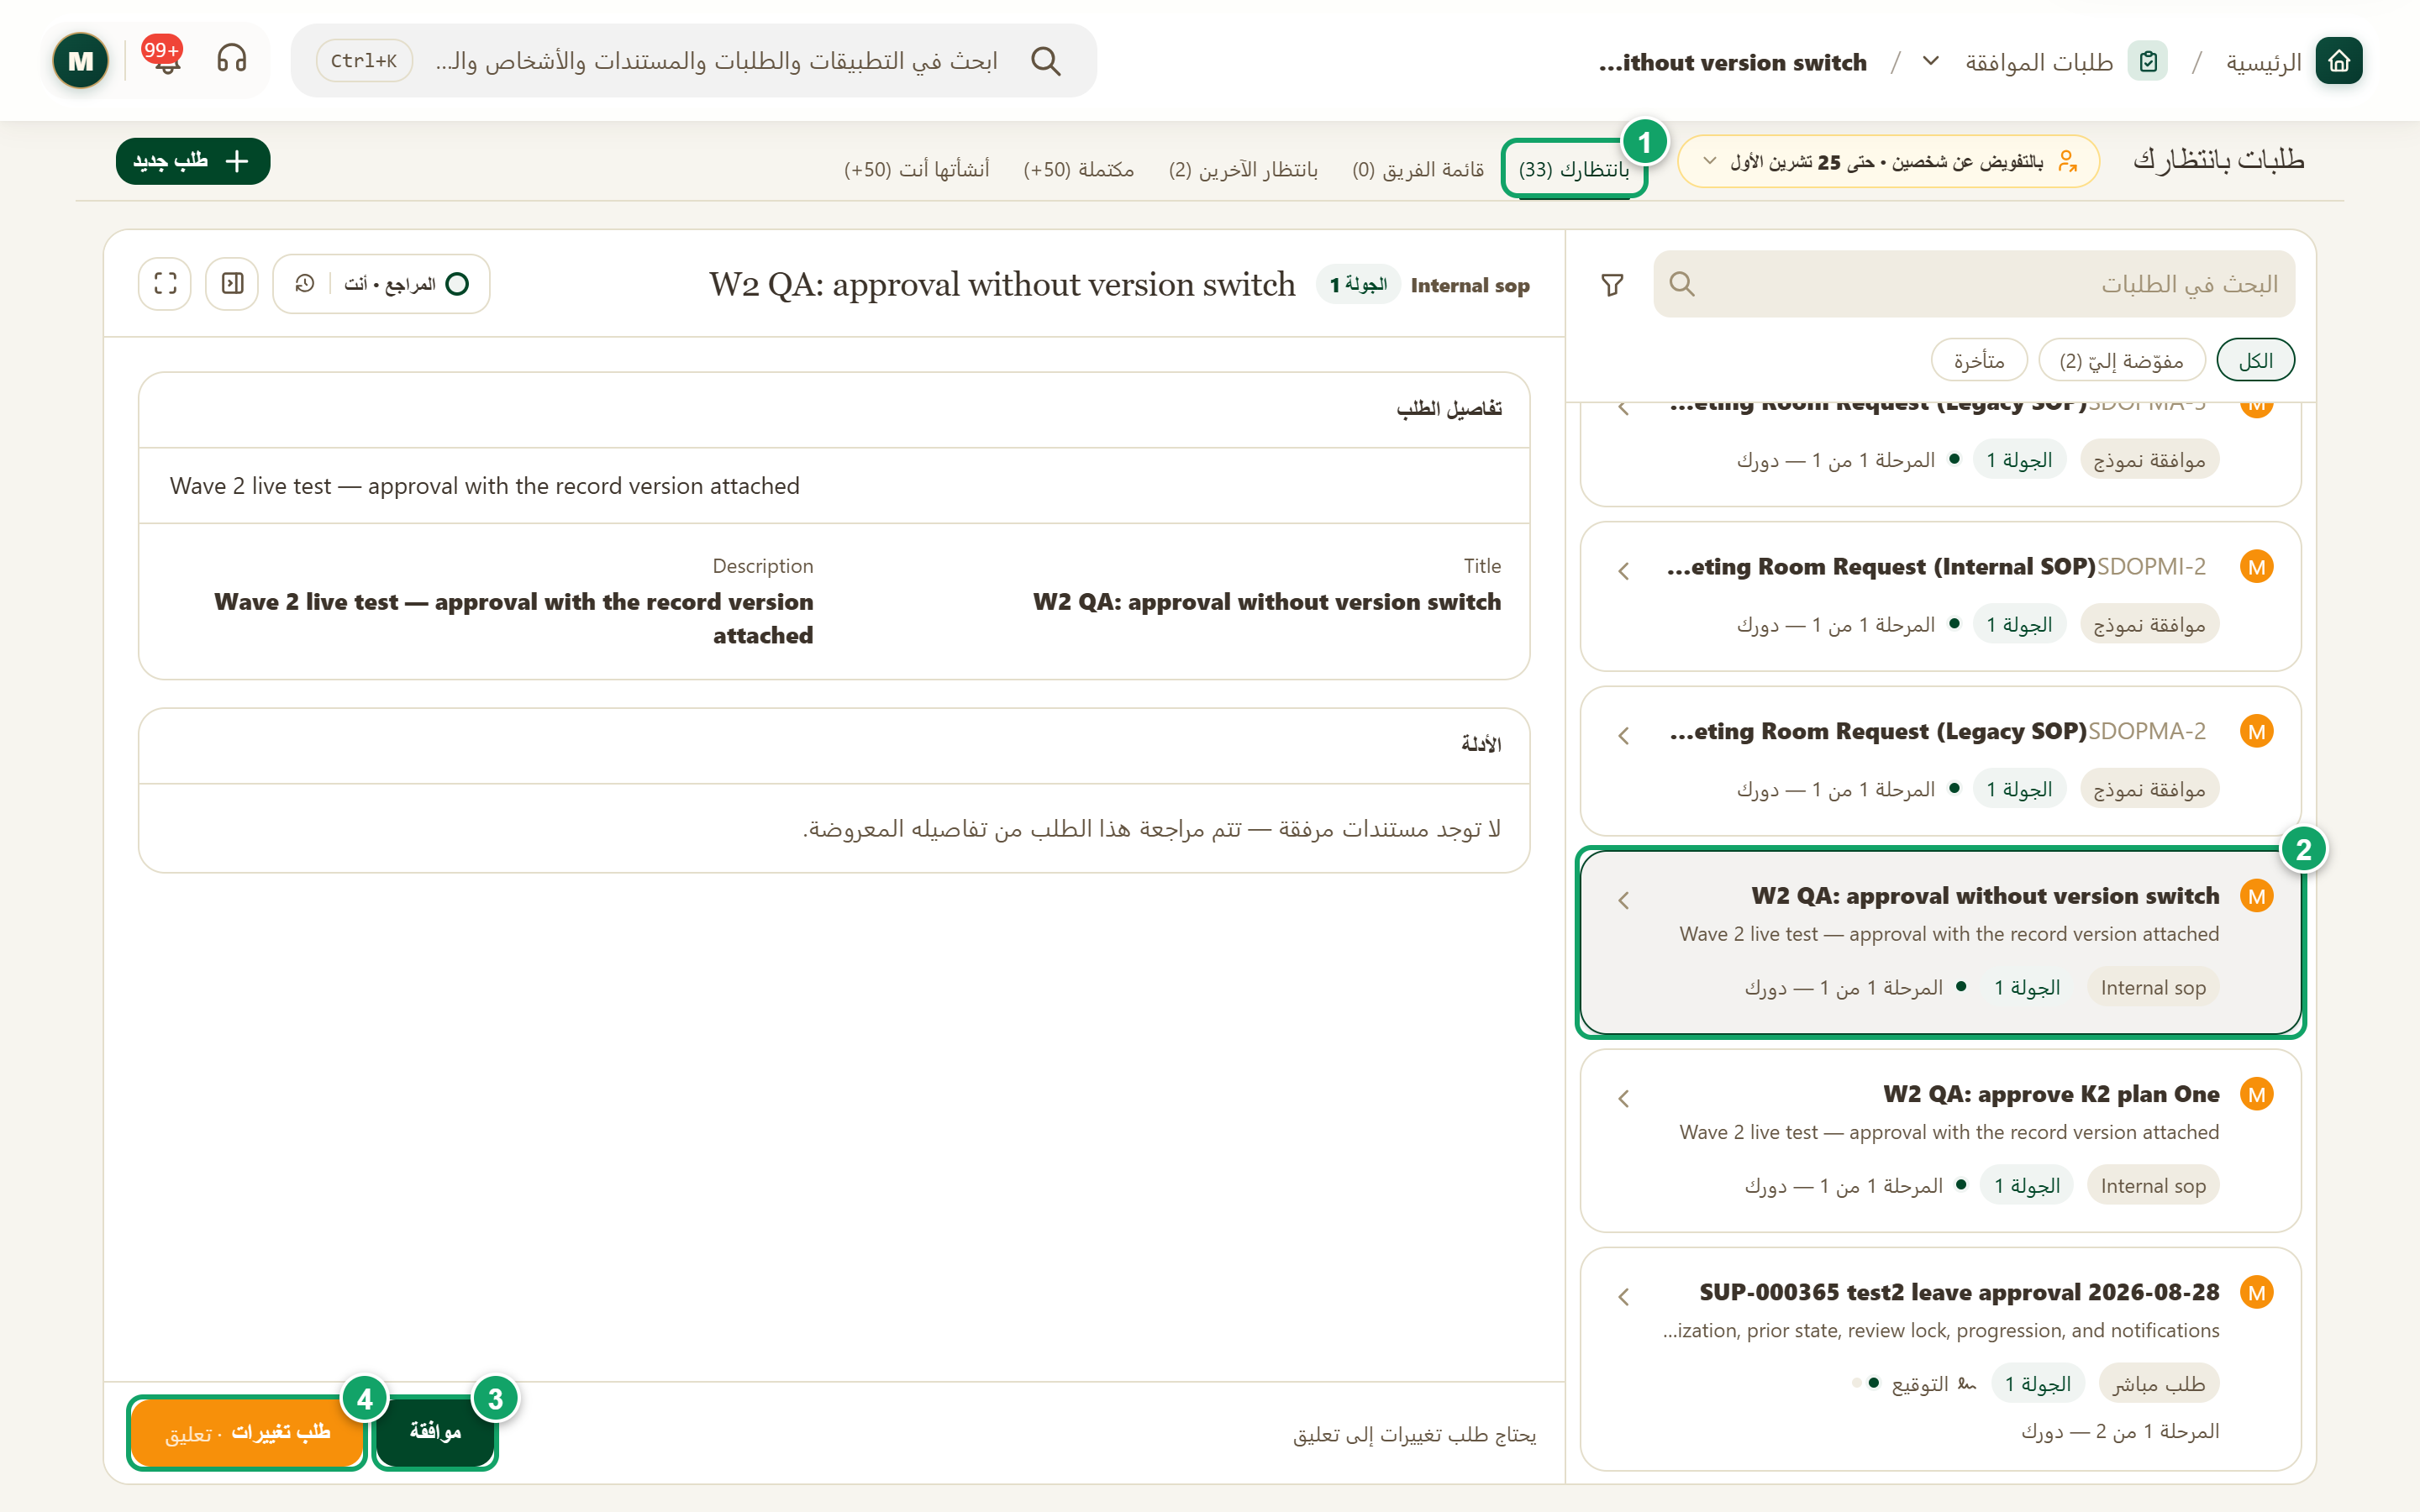
\includegraphics[width=0.95\linewidth,height=0.72\textheight,keepaspectratio]{figures/screens/ch06-isop-approvals-ar.png}
\caption{طلب موافقة من إجراء داخلي في «طلبات بانتظارك»}
\label{fig:builder-isop-approvals-screen}
\shotnote{تعرض الصورة صفحة «طلبات بانتظارك» في مؤسسة الاختبار، وقد اختير طلب أنشأته خطوة «طلب موافقة» من الإجراء الاختباري. وتظهر أزرار الرد بأسماء إجراءات الطلب التي حددها من بنى الخطوة، لذلك قد تختلف من إجراء إلى آخر. ① «بانتظارك»: التبويب الذي يجمع الطلبات المنتظرة لردك. ② بطاقة الطلب: تختارها لترى تفاصيله. ③ «موافقة»: إجراء الموافقة. ④ «طلب تغييرات»: إجراء يتطلب كتابة تعليق.}
\end{figure}

\begin{table}[H]
\centering
\caption{ما يحدث عند كل رد}
\label{tab:builder-isop-approvals-responses}
\begin{tabularx}{\linewidth}{R{3.6cm} Y}
\rcHeaderRow
\thh{الرد أو الحدث} & \thh{النتيجة}\\
الموافقة & الإجراء الجاهز في الخطوة، ويطلب توقيعاً ويكون التعليق اختيارياً. ويتابع الطلب إلى المرحلة التالية إن وُجدت.\\
طلب التغييرات & الإجراء الجاهز الثاني، والتعليق فيه إلزامي، وينهي الطلب بنتيجة طلب التغييرات.\\
انتهاء المهلة & إذا لم يصل رد خلال «المهلة الزمنية» انتهى الانتظار.\\
عند استجابة موافقة & مشغّل يبدأ إجراءً آخر مع كل رد على الطلب.\\
عند انتهاء موافقة & مشغّل يبدأ إجراءً آخر عندما يكتمل الطلب أو يُلغى أو تنتهي مهلته.\\
\end{tabularx}
\end{table}

\subsection{صفحة موافقات الإجراءات القديمة}

تبقى للإجراءات القديمة صفحة رد مستقلة يفتحها رابط الموافقة. وتعرض العنوان والتفاصيل وسياسة الموافقة وتاريخ الاستحقاق، وفيها «التعليق (اختياري)» بخمسمئة حرف على الأكثر، وزرّا «موافقة» و«رفض». ويُقبل رد واحد فقط، وتظهر حالة الطلب: «قيد الانتظار» أو «تمت الموافقة» أو «مرفوض» أو «منتهي الصلاحية» أو «ملغى».

\begin{figure}[H]
\centering
\begin{tikzpicture}[node distance=0.5cm]
\node[stepBox] (a) {\RL{خطوة طلب موافقة}};
\node[stepBox,below=of a] (b) {\RL{الطلب في طلبات بانتظارك}};
\node[stepBox,below=of b] (c) {\RL{رد المعتمد}};
\node[stepBox,below=of c] (d) {\RL{تسجيل النتيجة}};
\node[stepBox,below=of d] (e) {\RL{متابعة الإجراء}};
\draw[flowsTo] (a) -- (b);
\draw[flowsTo] (b) -- (c);
\draw[flowsTo] (c) -- (d);
\draw[flowsTo] (d) -- (e);
\end{tikzpicture}
\rclegend
\caption{رحلة طلب الموافقة}
\label{fig:builder-isop-approvals-flow}
\shotnote{يوضح المخطط أن الإجراء لا يقرر نيابةً عن المعتمد، بل يرسل الطلب وينتظر. فالنتيجة التي يسجلها الرد هي ما تقرؤه الخطوات التالية لتختار مسارها.}
\end{figure}

\subsection{خطوات العمل والتحقق}
\begin{enumerate}
\item افتح «طلبات بانتظارك»، واختر الطلب من تبويب «بانتظارك».
\item اقرأ عنوان الطلب وتفاصيله والسجل المرفق إن وُجد.
\item اضغط «موافقة» ووقّع، أو اضغط «طلب تغييرات» واكتب التعليق.
\item بصفتك من بنى الإجراء، افتح التشغيل في «عمليات التشغيل» وتحقق أنه تابع بعد الرد.
\end{enumerate}

\textbf{تحقق ومعالجة المشكلة:} يجب أن يخرج الطلب من «بانتظارك» ويظهر في «مكتملة»، وأن يتابع التشغيل بعد الرد. فإذا لم يجد المعتمد الطلب، فتأكد أنه في مراحل الموافقة، وأن التشغيل وصل فعلاً إلى خطوة «طلب موافقة». وإذا تأخر الرد، فأرسل تذكيراً من الطلب.

\clearpage
\section{المراجعة والنشر وسجل الإصدارات}
\label{sec:builder-feature-isop-publish}

لا يعمل الإجراء إلا بعد نشره، ولا تصل تعديلاتك إلى الإصدار المنشور حتى تنشرها من جديد. ويعرض «مراجعة ونشر» قبل النشر ما يجب إصلاحه، والتغييرات منذ الإصدار المنشور، ونتيجة آخر اختبار. وبعد النشر يُقفل الإصدار، فتكمل العمليات الجارية على إصدارها القديم، وتستخدم العمليات الجديدة الإصدار الجديد.

\textbf{المسار ومن يستخدمه:} المحرر ← «مراجعة ونشر»، وسجل الإصدارات من اسم الإجراء في رأس المحرر. يستخدمه من يبني الإجراء.

\begin{rcnote}[مثال: شركة الأفق]
يضيف المسؤول خطوة «إرسال إشعار» إلى الإجراء المنشور، فتظهر في «التغييرات منذ \en{v1} (المنشور)» بعلامة «مُضاف». فينشر \en{v2}، ويبقى طلب زيارة كان ينتظر موافقة سارة على \en{v1} حتى ينتهي.
\end{rcnote}

\begin{figure}[H]
\centering
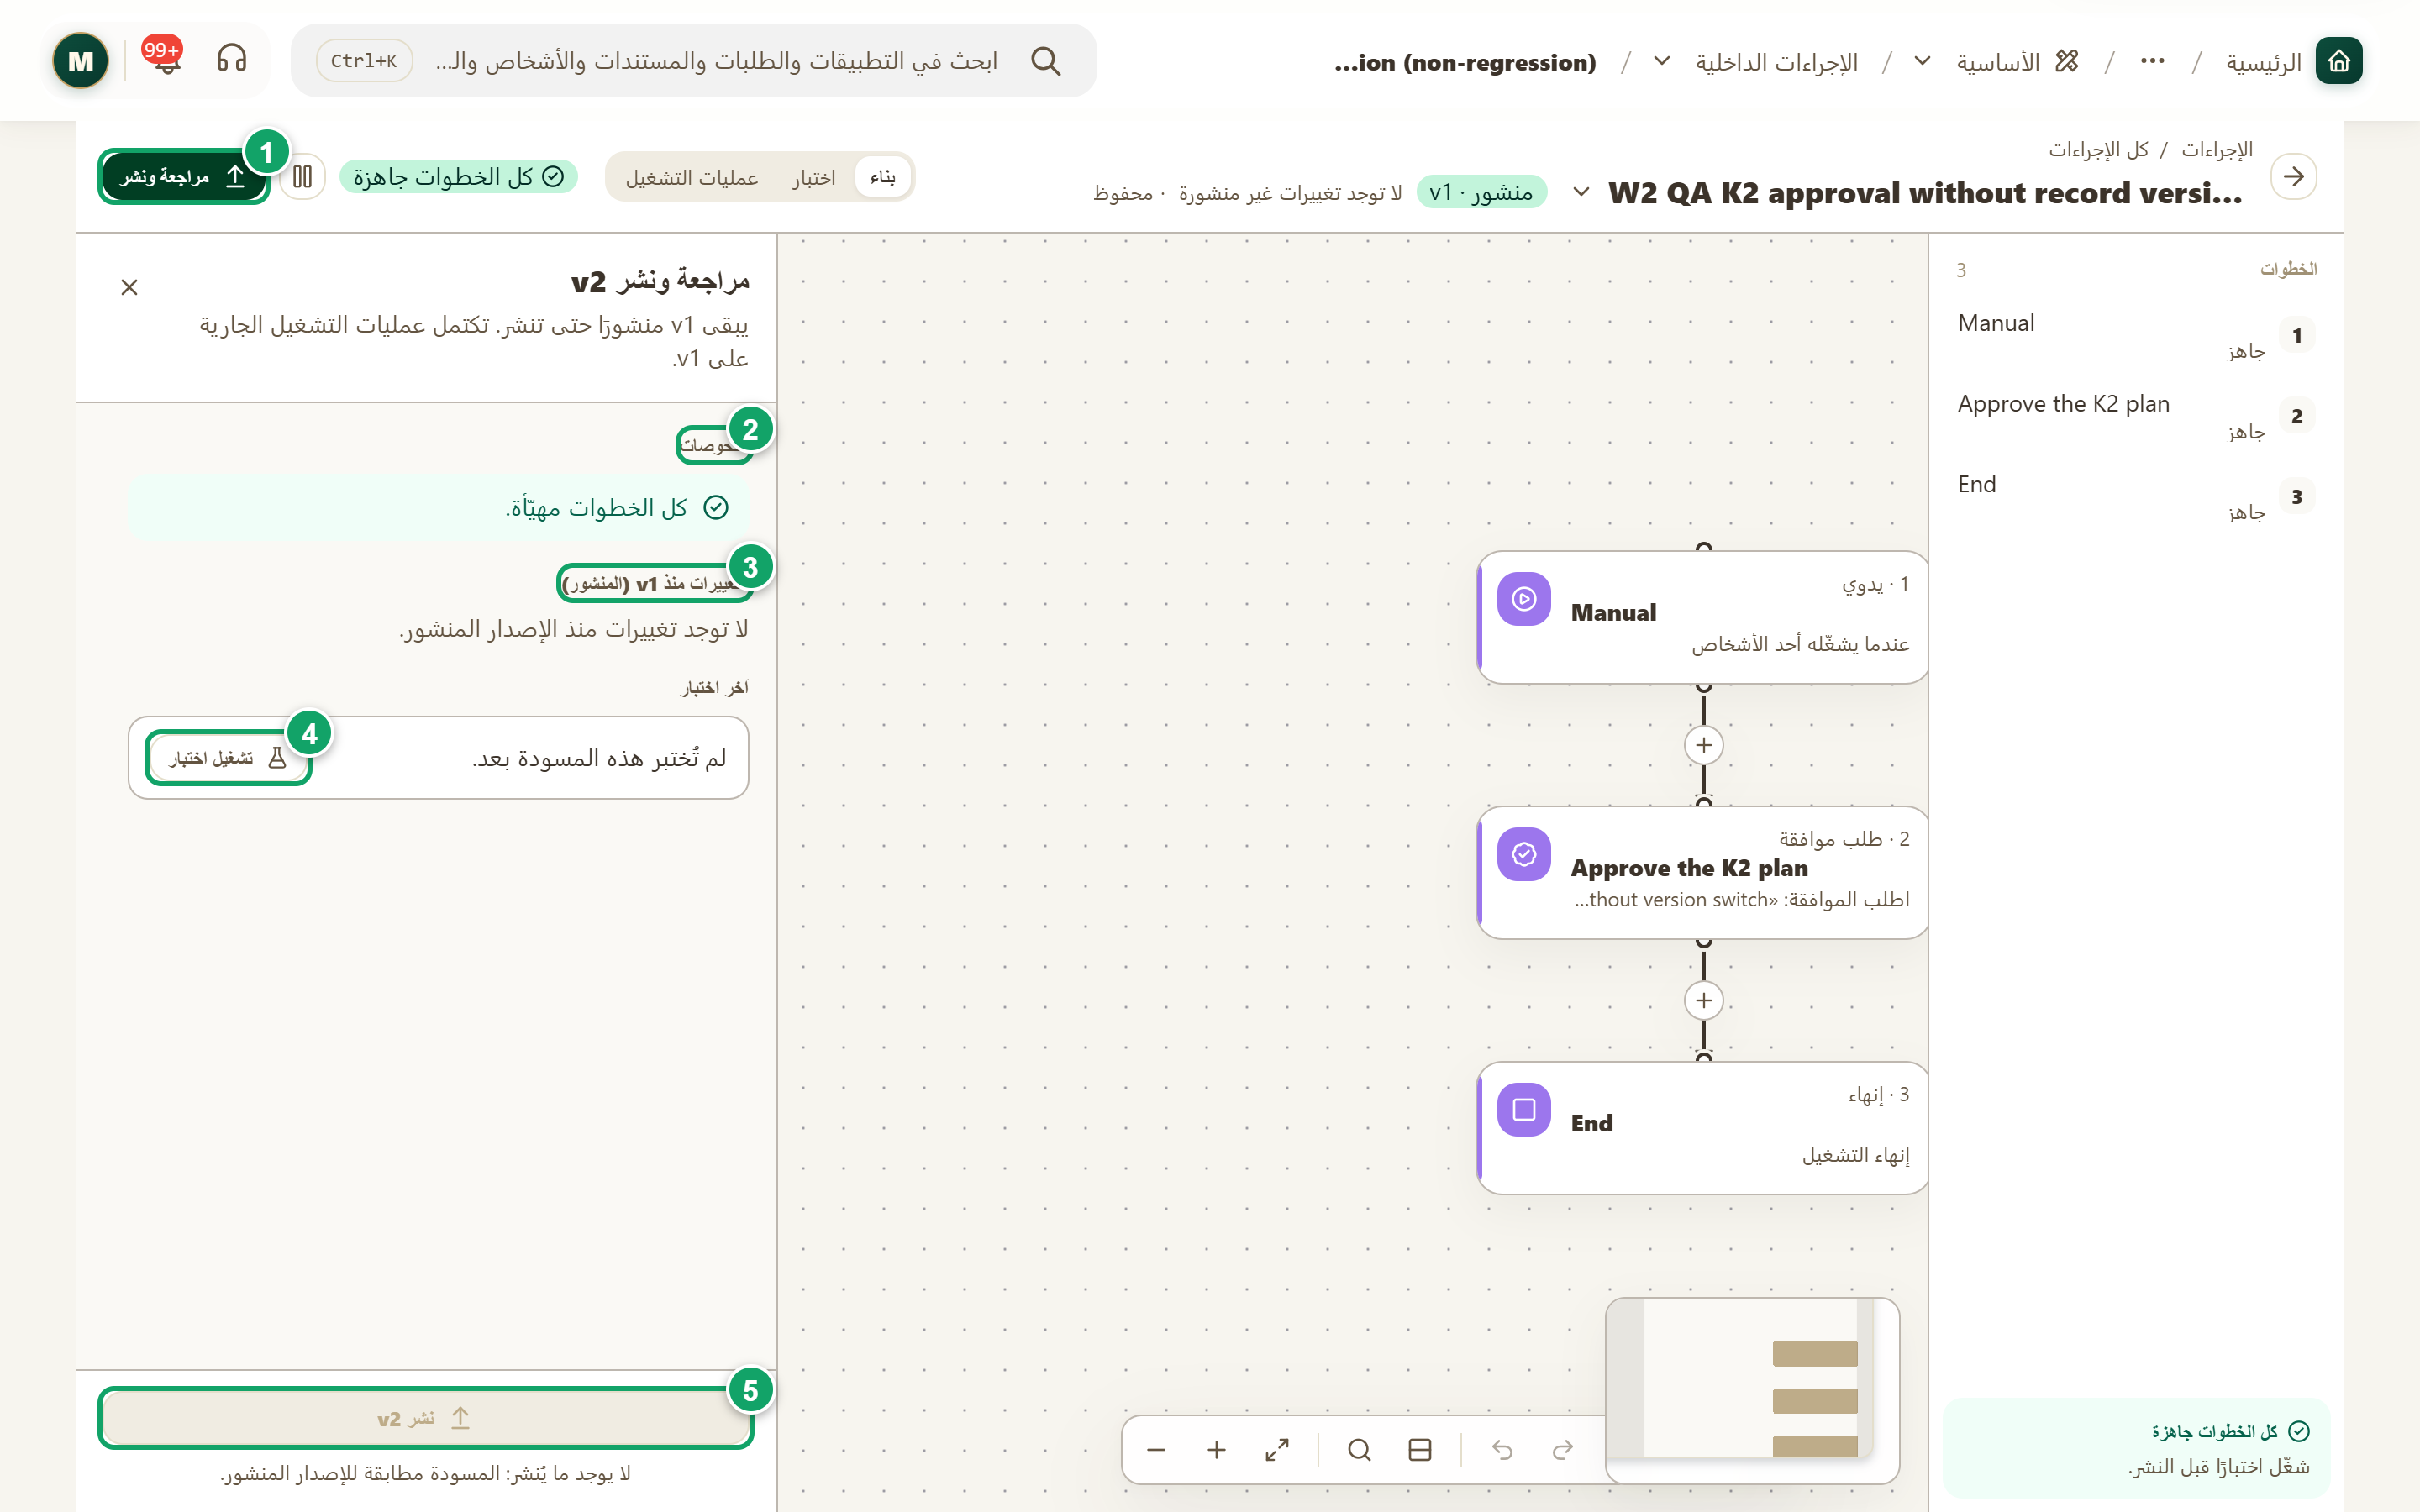
\includegraphics[width=0.95\linewidth,height=0.72\textheight,keepaspectratio]{figures/screens/ch06-isop-publish-ar.png}
\caption{لوحة «مراجعة ونشر v2» لإجراء منشور بلا تغييرات}
\label{fig:builder-isop-publish-screen}
\shotnote{تعرض الصورة لوحة المراجعة لإجراء منشور لم تتغير مسودته منذ \en{v1}، لذلك زر النشر معطّل وتحته سبب التعطيل. ولم يُنشر أي شيء عند الالتقاط؛ فاللوحة تبيّن ما تراجعه قبل النشر. ① «مراجعة ونشر»: يفتح اللوحة. ② «الفحوصات»: المشكلات التي تمنع النشر، أو تأكيد أن كل الخطوات مهيّأة. ③ «التغييرات منذ v1 (المنشور)»: ما تغيّر عن الإصدار المنشور. ④ «تشغيل اختبار»: يختبر المسودة قبل النشر. ⑤ «نشر v2»: ينشر الإصدار الجديد.}
\end{figure}

\begin{figure}[H]
\centering
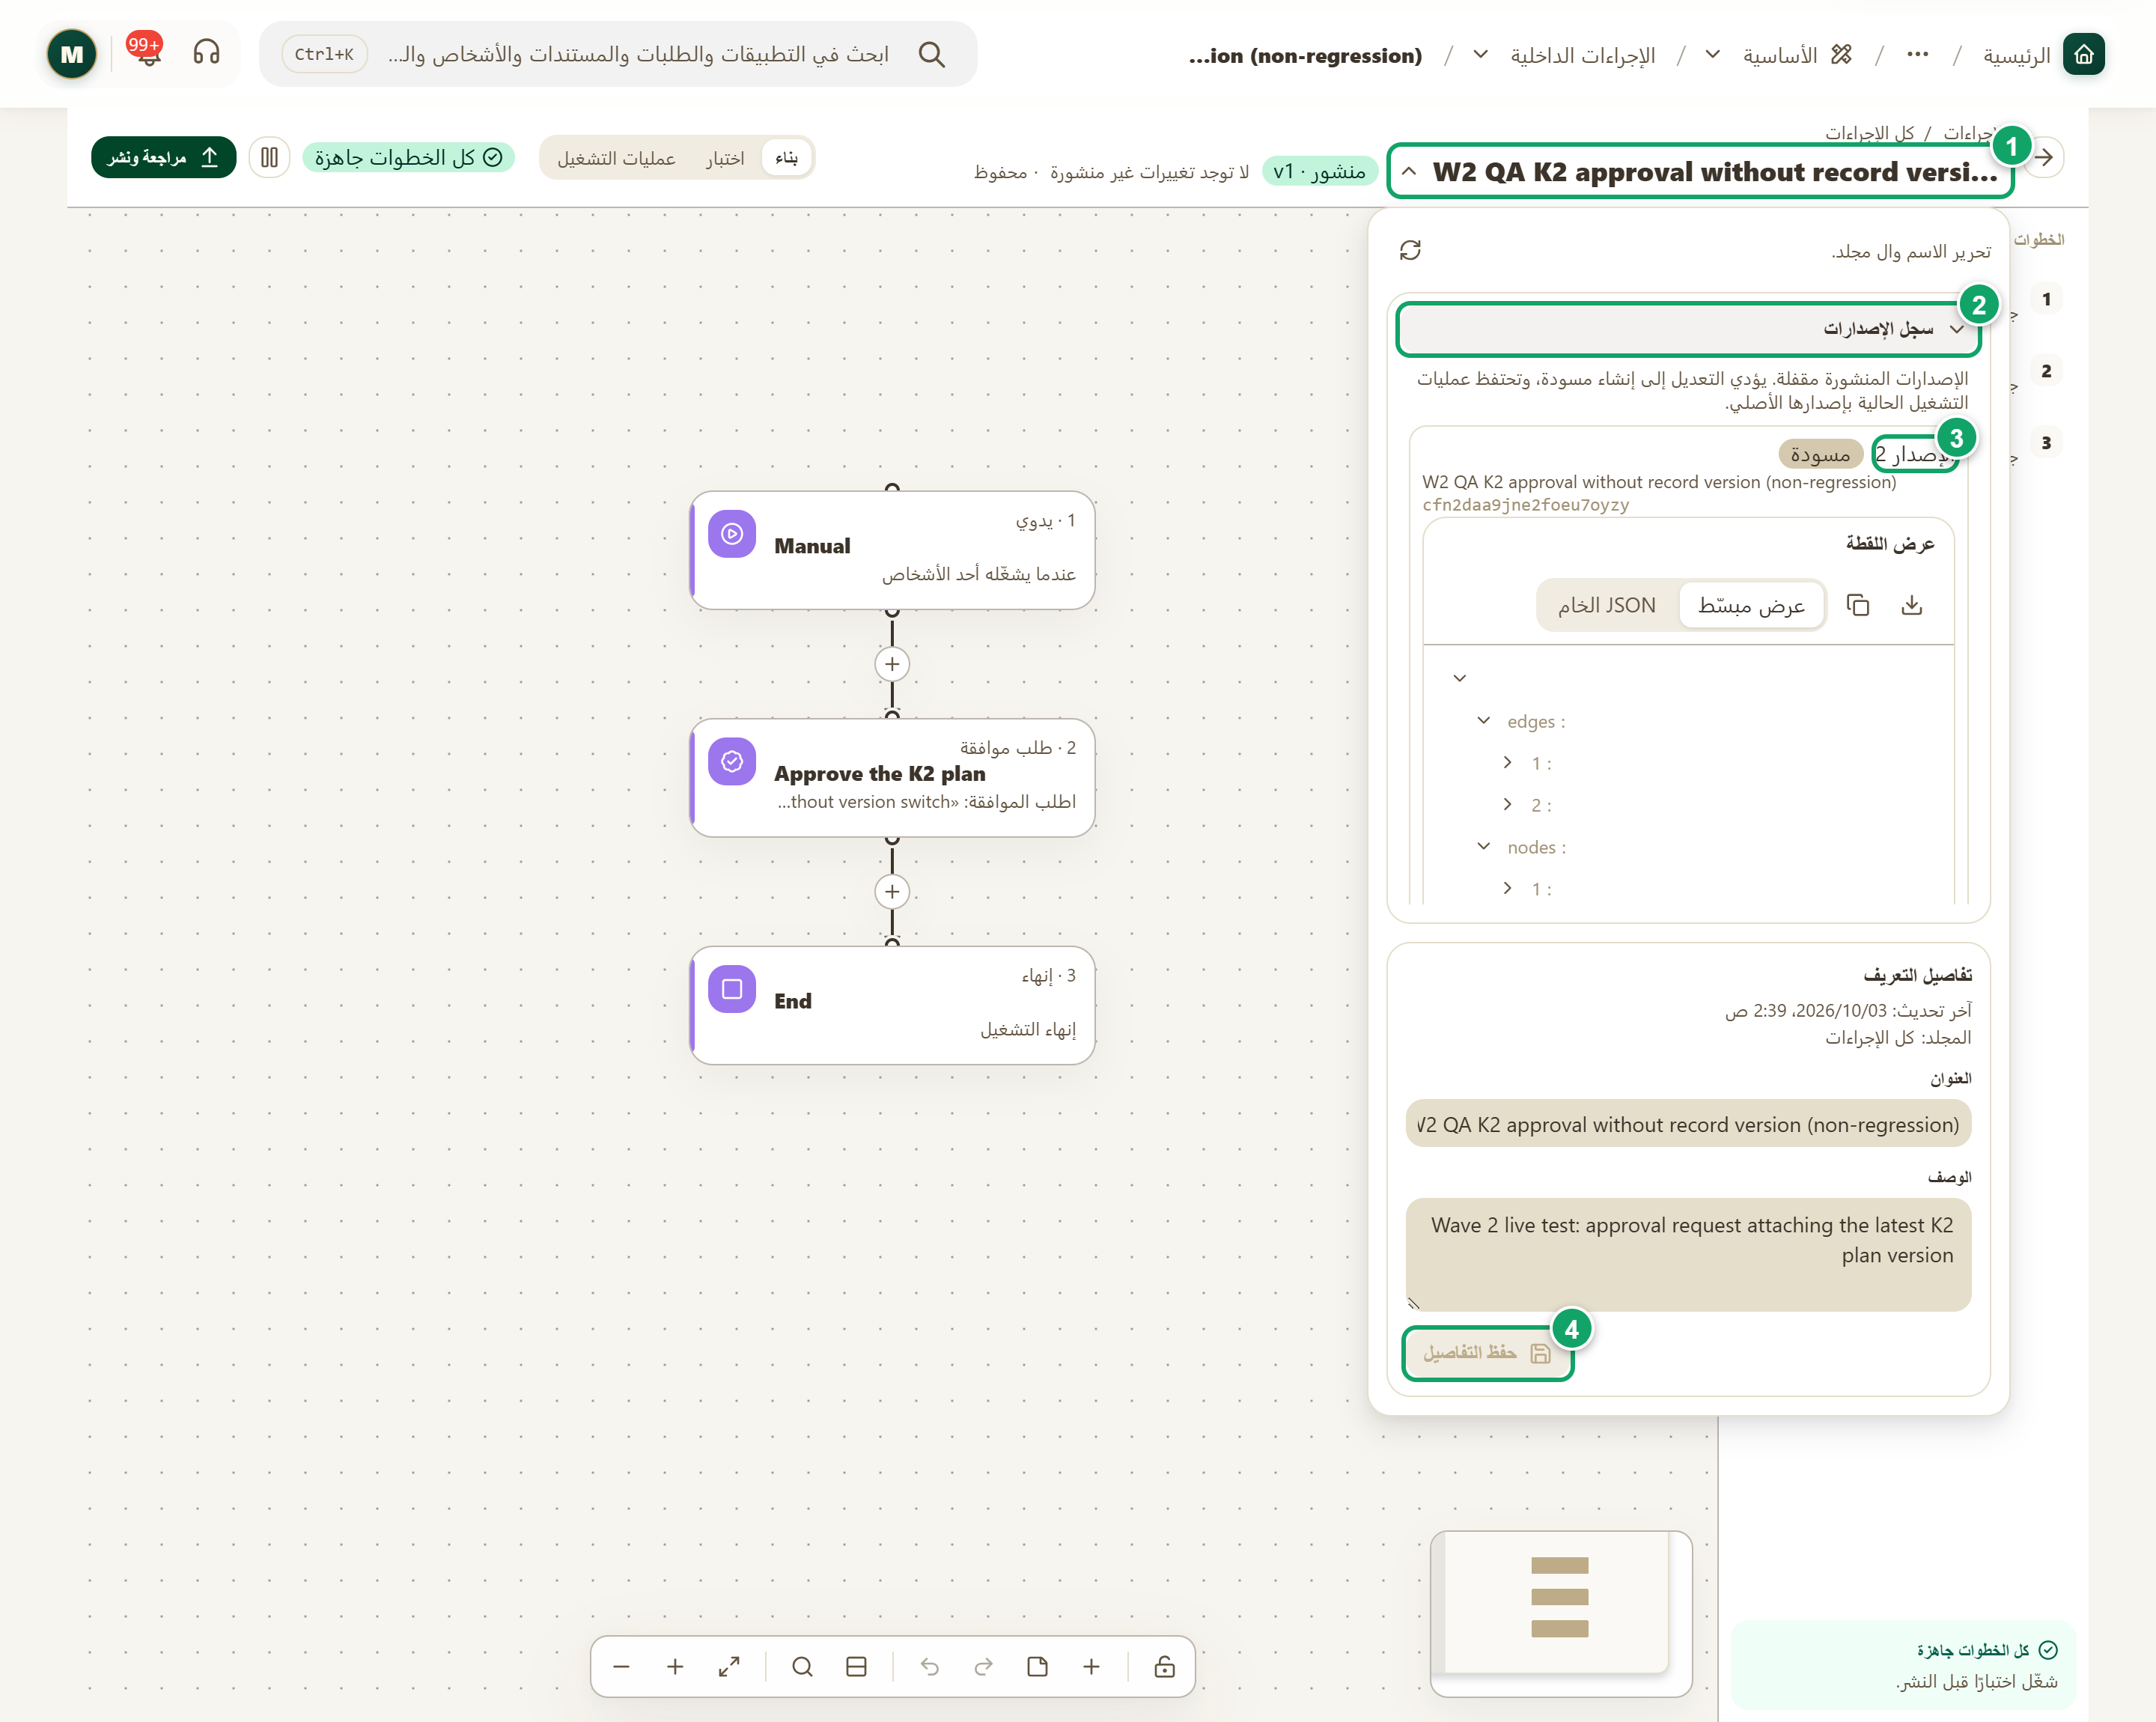
\includegraphics[width=0.95\linewidth,height=0.72\textheight,keepaspectratio]{figures/screens/ch06-isop-versions-ar.png}
\caption{سجل الإصدارات وتفاصيل التعريف}
\label{fig:builder-isop-publish-versions-screen}
\shotnote{تعرض الصورة القائمة التي تفتح من اسم الإجراء في رأس المحرر، وقد فُتح فيها «سجل الإصدارات» على المسودة الحالية مع لقطة تعريفها. وتذكّرك العبارة أعلى السجل بأن الإصدارات المنشورة مقفلة وأن التشغيل الجاري يبقى على إصداره. ① اسم الإجراء: يفتح هذه القائمة. ② «سجل الإصدارات»: يعرض الإصدارات ولقطاتها. ③ «الإصدار 2»: إصدار في السجل، وهو هنا مسودة. ④ «حفظ التفاصيل»: يحفظ العنوان والوصف بعد تعديلهما.}
\end{figure}

\begin{table}[H]
\centering
\caption{أقسام نافذة المراجعة}
\label{tab:builder-isop-publish-review}
\begin{tabularx}{\linewidth}{R{3.6cm} Y}
\rcHeaderRow
\thh{القسم} & \thh{ما يعرضه}\\
يجب إصلاحه قبل النشر & المشكلات التي تمنع النشر، ولكل منها زر «إصلاح» يفتح الخطوة. وعند خلوها يحمل القسم عنوان «الفحوصات» ويظهر فيه «كل الخطوات مهيّأة».\\
التغييرات منذ الإصدار المنشور & كل خطوة «مُضاف» أو «محذوف» أو «أُعيدت تسميته» أو «مُعدَّل»، وتغيّر «المسارات» بين الخطوات.\\
آخر اختبار & «نجح آخر اختبار لهذه المسودة» أو فشله أو «لم تُختبر هذه المسودة بعد»، مع «تشغيل اختبار». ويمكنك النشر دون اختبار، لكن الاختبار مستحسن.\\
زر النشر & «نشر \en{vN}». ويتعطل إذا بقيت مشكلات، أو كان الخادم غير متصل، أو لم يكن هناك ما يُنشر.\\
\end{tabularx}
\end{table}

\begin{table}[H]
\centering
\caption{بعد النشر}
\label{tab:builder-isop-publish-after}
\begin{tabularx}{\linewidth}{R{3.6cm} Y}
\rcHeaderRow
\thh{الأداة} & \thh{ما تفعله}\\
سجل الإصدارات & يعرض الإصدارات المنشورة المقفلة، ولكل منها «عرض اللقطة». والتعديل بعد النشر يُنشئ مسودة جديدة.\\
إيقاف الإجراء مؤقتًا & يمنع المشغّلات من بدء عمليات جديدة حتى «استئناف»، دون أن يحذف الإجراء أو إصداراته.\\
تفاصيل التعريف & تعدّل «العنوان» و«الوصف» ثم تضغط «حفظ التفاصيل».\\
\end{tabularx}
\end{table}

\begin{figure}[H]
\centering
\begin{tikzpicture}[node distance=0.5cm]
\node[stepBox] (a) {\RL{مسودة مكتملة}};
\node[stepBox,below=of a] (b) {\RL{مراجعة ونشر}};
\node[stepBox,below=of b] (c) {\RL{إصلاح المشكلات}};
\node[stepBox,below=of c] (d) {\RL{نشر الإصدار}};
\node[stepBox,below=of d] (e) {\RL{إصدار مقفل في السجل}};
\draw[flowsTo] (a) -- (b);
\draw[flowsTo] (b) -- (c);
\draw[flowsTo] (c) -- (d);
\draw[flowsTo] (d) -- (e);
\end{tikzpicture}
\rclegend
\caption{من المسودة إلى إصدار منشور}
\label{fig:builder-isop-publish-flow}
\shotnote{يبيّن المخطط أن كل نشر يُنتج إصداراً مقفلاً جديداً بدلاً من تعديل الإصدار السابق. لذلك لا يتأثر تشغيل بدأ قبل النشر، وتستطيع دائماً أن تعرف الإصدار الذي عمل عليه كل تشغيل.}
\end{figure}

\subsection{خطوات العمل والتحقق}
\begin{enumerate}
\item اضغط «مراجعة ونشر» في رأس المحرر.
\item اضغط «إصلاح» بجانب كل مشكلة، وأصلح الخطوة، ثم عُد إلى المراجعة.
\item راجع «التغييرات منذ» الإصدار المنشور، وشغّل اختباراً إن لم تختبر المسودة.
\item اضغط «نشر \en{vN}».
\item لمراجعة إصدار سابق، اضغط اسم الإجراء في رأس المحرر وافتح «سجل الإصدارات».
\end{enumerate}

\textbf{تحقق ومعالجة المشكلة:} يجب أن تظهر رسالة «أصبح \en{vN} منشورًا»، وأن تتغير شارة الإصدار إلى «منشور · \en{vN}». فإذا ظهر «لا يوجد ما يُنشر: المسودة مطابقة للإصدار المنشور»، فلم تغيّر شيئاً منذ آخر نشر. وإذا ظهر «تغيّرت المسودة أثناء النشر»، فانشر مرة أخرى لتشمل آخر تعديلاتك.


\chapter{إجراءات التشغيل القياسية والبوتات}
\label{ch:builder-automations}

\section{ماذا ستبني في هذا الفصل؟}
\label{sec:builder-automations-intro}

يجمع هذا الفصل أداتين تربطان كيان بما حوله. فصفحة «إجراءات التشغيل القياسية» تفتح استوديو أتمتة مضمّناً يبني مسارات تبدأ بحدث في كيان، ثم تقرأ البيانات وتتحقق منها، وتنفّذ إجراءً تترك نتيجته أثراً يمكن مراجعته. أما صفحة «البوتات» فتُعدّ مساعدين لهم اسم وصورة، وتحدد أين يضيفهم الأعضاء في الدردشة والبريد والتقويم، وهل يُثبَّتون تلقائياً.

ويشرح الفصل الأتمتة على خمس صفحات تتبع ترتيب البناء: الفكرة العامة، ثم المشغّلات، ثم الإجراءات، ثم الاتصالات، ثم الاختبار ومعالجة الأعطال. وتأتي بعدها صفحتا البوتات: قدراته، ثم تثبيته الافتراضي.

\begin{rcnote}[مثال: شركة الأفق]
يبني مسؤول النظام في الأفق أتمتة تنشئ مهمة مراجعة لسارة الخطيب كلما أرسل عمر حداد طلب زيارة جديداً في «طلبات الزيارة». ويُعدّ كذلك بوت «مساعد الزيارات» ويضيفه إلى قناة الفروع، فيذكره عمر في المحادثة عندما يحتاج إلى متابعة طلبه.
\end{rcnote}

\section{صفحات هذا الفصل}
\label{sec:builder-automations-pages}

الصفحتان الرئيسيتان مستقلتان في قسم «الأساسية» من أدوات البناء، أما بقية الصفحات فتشرح أجزاء داخلهما. فاتبع الترتيب في المرة الأولى، ثم عُد إلى أي صفحة عندما تحتاج إليها.

\begin{table}[H]
\centering
\caption{الأتمتة والبوتات خطوة بخطوة}
\label{tab:builder-pages-automations}
\rcZebra
\begin{tabularx}{\linewidth}{R{4.2cm} Y}
\rcHeaderRow
\thh{الصفحة وقسمها} & \thh{ماذا تقدم هذه الصفحة؟}\\
إجراءات التشغيل القياسية — الأساسية & تشرح استوديو الأتمتة ونموذج المسار من الحدث إلى النتيجة التي تُراجَع.\\
مشغّلات الأتمتة — إجراءات التشغيل القياسية & تعرض الأحداث التي تبدأ الأتمتة، وكيف تختار أضيقها وتمنع تكرار التشغيل.\\
إجراءات الأتمتة — إجراءات التشغيل القياسية & تعرض ما تستطيع الأتمتة فعله بالسجلات والمهام والنماذج والمستندات والإشعارات.\\
اتصالات الأتمتة — إجراءات التشغيل القياسية & تشرح الاتصال الذي تعمل الأتمتة من خلاله، ومن يملكه، وكيف تعالج أخطاءه.\\
اختبار الأتمتة وتشغيلها ومعالجة أعطالها — إجراءات التشغيل القياسية & تشرح اختبار كل جزء قبل التفعيل، وترتيب البحث عن سبب العطل.\\
البوتات — الأساسية & تعرض بوتات المؤسسة، وتحدد أين يضيفها الأعضاء في الدردشة والبريد والتقويم.\\
التثبيت الافتراضي للبوت — البوتات & تحدد هل يُضاف البوت تلقائياً، وهل يستطيع الأعضاء إزالته، وما البريد الذي يصل إليه.\\
\end{tabularx}
\end{table}

\clearpage
\section{إجراءات التشغيل القياسية}
\label{sec:builder-feature-sops}

تفتح هذه الصفحة استوديو أتمتة مضمّناً يبني مسارات تربط كيان بحسابات وخدمات أخرى، وتبدأ بحدث في كيان مثل إنشاء سجل أو إرسال نموذج. وتعمل كل أتمتة فيه من خلال اتصال بحساب كيان تختاره أولاً. أما مسارات الاعتماد والمهام داخل المؤسسة فالأنسب لها «الإجراءات الداخلية».

\textbf{المسار ومن يستخدمه:} «ادوات البناء» ← «الأساسية» ← «إجراءات التشغيل القياسية». يستخدمها من يملك صلاحية النماذج ويحتاج إلى ربط كيان بأنظمة أخرى.

\begin{rcnote}[مثال: شركة الأفق]
تريد الأفق أن تصل رسالة إلى جدول متابعة خارجي كلما أُنشئ طلب زيارة. لذلك يبني مسؤول النظام أتمتة تبدأ عند إنشاء سجل جديد في «طلبات الزيارة»، ثم تتحقق من الفرع قبل أن ترسل البيانات.
\end{rcnote}

\begin{table}[H]
\centering
\caption{أجزاء الأتمتة}
\label{tab:builder-sops-parts}
\begin{tabularx}{\linewidth}{R{3.6cm} Y}
\rcHeaderRow
\thh{الجزء} & \thh{المعنى}\\
الاتصال & حساب كيان الذي تعمل الأتمتة باسمه، ويُختار أولاً. اجعله بأقل صلاحيات تكفي العمل.\\
المشغّل & الحدث الذي يبدأ الأتمتة، مثل إنشاء سجل أو تحديثه أو إجراء على نموذج أو مهمة.\\
الشرط & يتحقق من البيانات قبل أي كتابة، حتى لا تعمل الأتمتة على سجلات لا تخصها.\\
الإجراءات & ما تفعله الأتمتة: إنشاء سجل أو تحديثه أو البحث عنه، وإنشاء مهام، وإرسال إشعار، وغيرها.\\
\end{tabularx}
\end{table}

\begin{figure}[H]
\centering
\begin{tikzpicture}[node distance=0.5cm]
\node[stepBox] (a) {\RL{اختيار الاتصال}};
\node[stepBox,below=of a] (b) {\RL{المشغّل}};
\node[stepBox,below=of b] (c) {\RL{شرط قبل الكتابة}};
\node[stepBox,below=of c] (d) {\RL{إجراء واحد في كل مرة}};
\draw[flowsTo] (a) -- (b);
\draw[flowsTo] (b) -- (c);
\draw[flowsTo] (c) -- (d);
\end{tikzpicture}
\rclegend
\caption{ترتيب بناء الأتمتة}
\label{fig:builder-sops-flow}
\shotnote{يضع المخطط الشرط قبل الإجراء، لأن الأتمتة التي تكتب دون تحقق قد تغيّر سجلات كثيرة في لحظة. وتُختبر الأجزاء واحداً واحداً: المشغّل وحده، ثم الشرط في الحالتين، ثم كل إجراء على حدة.}
\end{figure}

\subsection{خطوات العمل والتحقق}
\begin{enumerate}
\item افتح «إجراءات التشغيل القياسية» وأنشئ مساراً جديداً، ثم اختر اتصال كيان.
\item اختر المشغّل، واختبره ببيانات عينة.
\item أضف شرطاً يتحقق من البيانات، ثم أضف الإجراءات واحداً بعد الآخر واختبر كلاً منها.
\item فعّل الأتمتة بعد نجاح الاختبار، ثم راجع أول تشغيل فعلي.
\end{enumerate}

\textbf{تحقق ومعالجة المشكلة:} يجب أن يظهر التشغيل في سجل الأتمتة بالنتيجة المتوقعة. فإذا ظهرت الصفحة فارغة أو برسالة خطأ، فقد تكون خدمة الأتمتة غير متاحة في بيئة مؤسستك؛ وفي بيئة الاختبار \en{test2} ظهرت الصفحة فارغة عند التحقق. وإذا فشل إجراء، فراجع صلاحيات الاتصال أولاً.

\clearpage
\section{البوتات}
\label{sec:builder-feature-bots}

البوت مساعد له اسم وصورة، يضيفه الأعضاء إلى الدردشة أو البريد أو التقويم. وتحدد في هذه الصفحة أين يمكن إضافته، وهل يُضاف تلقائياً، وكيف يصل إلى البريد. أما ما يفعله البوت عندما يُراسَل أو يُذكر فيُبنى في «الإجراءات الداخلية» بمشغّلات مثل «عند رسالة مباشرة إلى الروبوت» و«عند الإشارة».

\textbf{المسار ومن يستخدمه:} «ادوات البناء» ← «الأساسية» ← «البوتات». يستخدمها من يملك صلاحية البوتات.

\begin{rcnote}[مثال: شركة الأفق]
ينشئ مسؤول النظام بوت «مساعد الزيارات»، ويجعله قابلاً للإضافة إلى الدردشات المباشرة. فإذا راسله عمر حداد، بدأ إجراء داخلي يرد عليه بحالة طلب زيارته. ويبدأ البوت من ①.
\end{rcnote}

\begin{figure}[H]
\centering
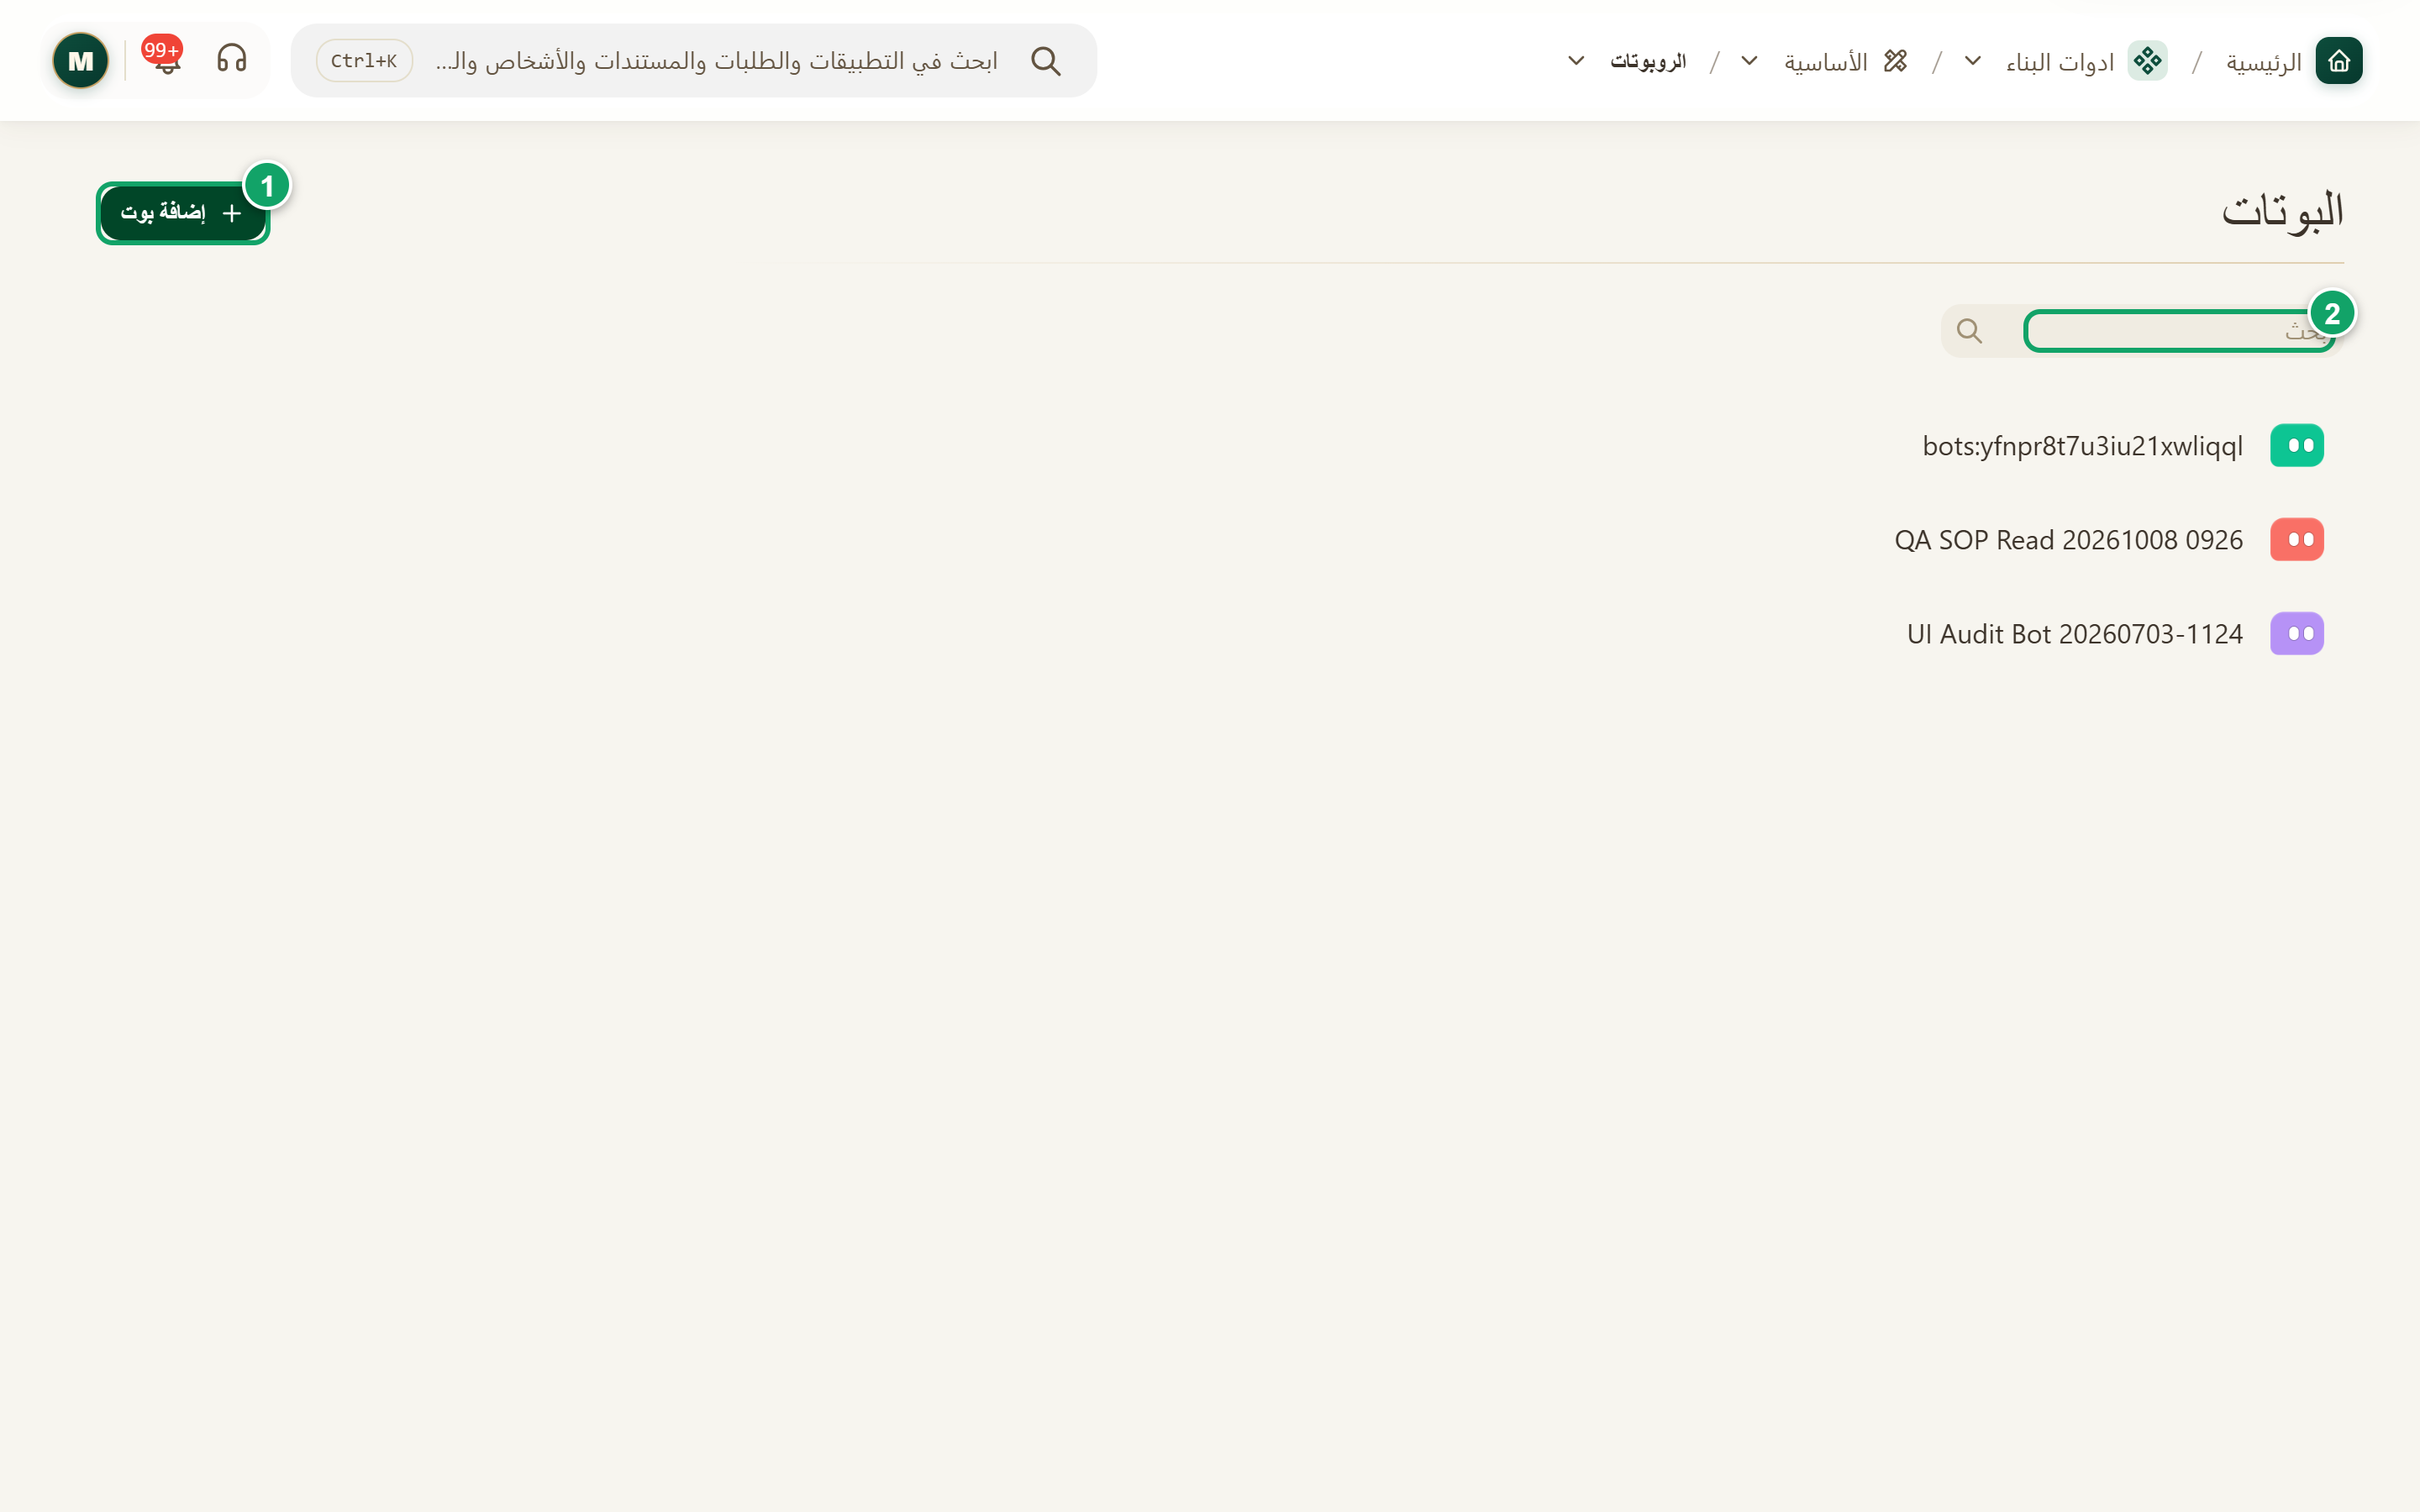
\includegraphics[width=0.95\linewidth,height=0.72\textheight,keepaspectratio]{figures/screens/ch06-bots-ar.png}
\caption{صفحة «البوتات»}
\label{fig:builder-bots-screen}
\shotnote{تعرض الصفحة البوتات المعرّفة في المؤسسة، وهي هنا بوتات اختبار. ① «إضافة بوت»: يطلب الاسم فقط. ② البحث: يجد البوت بالاسم.}
\end{figure}


\begin{table}[H]
\centering
\caption{إعدادات البوت}
\label{tab:builder-bots-data}
\begin{tabularx}{\linewidth}{R{3.6cm} Y}
\rcHeaderRow
\thh{القسم} & \thh{ماذا تحدد؟}\\
إضافة بوت & يطلب الاسم فقط، وتُختار صورته تلقائياً.\\
الدردشة & هل يُضاف إلى الدردشات المباشرة أو القنوات، وهل يمكن مراسلته أو ذكره.\\
البريد الإلكتروني & هل يُثبّت في البريد، وهل يمكن إضافته في نسخة، وإضافة جهات اتصال داخلية أو خارجية.\\
التقويم & هل يمكن تثبيته في التقويم.\\
التثبيت الافتراضي & هل يُضاف تلقائياً إلى الدردشة أو البريد أو التقويم، وحدود وصوله الافتراضية إلى البريد.\\
\end{tabularx}
\end{table}

\begin{figure}[H]
\centering
\begin{tikzpicture}[node distance=0.5cm]
\node[entity] (bot) {\RL{البوت}};
\node[entityOpt,below right=0.7cm and 0.3cm of bot] (where) {\RL{أين يُضاف}};
\node[entityOpt,below left=0.7cm and 0.3cm of bot] (sop) {\RL{إجراء داخلي يرد}};
\draw[dependsOnOpt] (bot.south) -- ++(0,-0.3) -| (where.north);
\draw[dependsOnOpt] (bot.south) -- ++(0,-0.3) -| (sop.north);
\end{tikzpicture}
\rclegend
\caption{هوية البوت وعمله}
\label{fig:builder-bots-model}
\shotnote{يفصل الشكل بين أمرين: هذه الصفحة تحدد هوية البوت وأماكن إضافته، أما ردوده فيبنيها إجراء داخلي يبدأ عندما يُراسَل البوت أو يُذكر. لذلك لا يفعل البوت شيئاً وحده حتى تربطه بإجراء منشور.}
\end{figure}

\subsection{خطوات العمل والتحقق}
\begin{enumerate}
\item افتح «البوتات» واضغط «إضافة بوت»، ثم اكتب الاسم واضغط «إنشاء».
\item افتح البوت، وفعّل أماكن إضافته في الدردشة والبريد والتقويم، ثم اضغط «حفظ».
\item ابنِ في «الإجراءات الداخلية» إجراءً يبدأ «عند رسالة مباشرة إلى الروبوت» وانشره.
\end{enumerate}

\textbf{تحقق ومعالجة المشكلة:} أضف البوت إلى دردشة تجريبية وأرسل إليه رسالة، فيجب أن يبدأ الإجراء ويظهر في «عمليات التشغيل». فإذا لم تظهر خيارات الإضافة للأعضاء، فراجع إعدادات الدردشة والحفظ؛ وإذا لم يرد البوت، فتأكد من أن الإجراء منشور وغير متوقف.


\chapter{المستندات والطباعة}
\label{ch:builder-documents}

\section{ماذا ستبني في هذا الفصل؟}
\label{sec:builder-documents-intro}

يحتاج العمل غالباً إلى مستند رسمي يُستخرج من بيانات السجل، مثل خطاب أو كشف أو نموذج مطبوع. ويقدّم كيان ثلاث طرق لإنشاء هذه المستندات: قوالب Word التي تكتبها في برنامج Word وترفعها، وقوالب Excel التي تناسب الكشوف والجداول، وقوالب الطباعة التي تصممها داخل كيان دون أي ملف خارجي. ويشرح الفصل كل طريقة على صفحات قصيرة: إنشاء القالب، ثم كتابة وسومه أو عناصره، ثم اختباره ونشره.

وتعتمد قوالب الطباعة على الهويات والترويسات، وهي شعار المؤسسة واسمها وبياناتها الرسمية ورأس الصفحة وتذييلها. لذلك يختم الفصل بصفحتين عنهما، وفي إحداهما محرر الترويسة. وإذا كانت مستنداتك رسمية فابدأ بالهوية والترويسة، ثم اختر نوع القالب الذي يناسب المستند.

\begin{rcnote}[مثال: شركة الأفق]
تُعدّ الأفق ثلاثة مستندات لطلبات الزيارة: خطاب تأكيد بصيغة Word، وكشفاً شهرياً لزيارات الفرع بصيغة Excel، وورقة زيارة مطبوعة على ترويسة الشركة فيها رمز QR. فتطبع سارة الخطيب الورقة بعد مراجعة الطلب HZN-VR-0001، ويتحقق فرع حلب من صحتها بمسح الرمز.
\end{rcnote}

\section{صفحات هذا الفصل}
\label{sec:builder-documents-pages}

تبدأ صفحات Word وExcel والطباعة كلها من قسم «الأساسية» في أدوات البناء. أما منشئ قالب الطباعة فيُفتح من داخل منشئ النموذج أو نوع السجلات، وصفحة التحقق صفحة عامة يفتحها رمز QR.

\begin{table}[H]
\centering
\caption{المستندات والطباعة}
\label{tab:builder-pages-documents}
\rcZebra
\begin{tabularx}{\linewidth}{R{4.2cm} Y}
\rcHeaderRow
\thh{الصفحة وقسمها} & \thh{ماذا تقدم هذه الصفحة؟}\\
قوالب DOCX — الأساسية & قائمة قوالب Word وطريقة إنشاء قالب جديد برفع ملف أو بمساعدة الذكاء الاصطناعي.\\
وسوم قوالب DOCX والتكرار — الأساسية & كتابة الوسوم في Word: القيم والشروط والتكرار والصور والروابط ورموز QR.\\
مساحة عمل قالب DOCX ومساعد الذكاء الاصطناعي — الأساسية & الإعدادات والإصدارات والاختبار، وتعديل القالب بمساعد يقترح مسودة تراجعها قبل الحفظ.\\
قوالب XLSX — الأساسية & قائمة قوالب Excel وطريقة إنشاء قالب جديد برفع مصنف.\\
وسوم قوالب XLSX والطباعة — الأساسية & تكرار الصفوف والأعمدة، والمصفوفات، والتوجيهات، والصيغ، وإعداد الطباعة.\\
مساحة عمل قالب XLSX — الأساسية & الإعدادات، واستبدال المصنف، واختبار الإخراج بصيغة Excel أو PDF، ومساعد المصنف.\\
قوالب الطباعة — الأساسية & مكتبة قوالب الطباعة ونافذة «قوالب الطباعة» داخل منشئ النموذج أو النوع.\\
منشئ قالب الطباعة: البيانات والعناصر — منشئ النموذج أو نوع السجلات & وضع الحقول والعناصر على الصفحة وضبط طريقة طباعة كل منها.\\
إعدادات الصفحة في قالب الطباعة — منشئ النموذج أو نوع السجلات & الورق والاتجاه واللغة والهوامش والهوية والترويسة والعلامة المائية.\\
المعاينة والنشر والطباعة من السجل — منشئ النموذج أو نوع السجلات & المعاينة بسجل حقيقي، وإعدادات المخرجات، والنشر، وزر «طباعة» في السجل.\\
صفحة التحقق من المستند — صفحة عامة & الصفحة التي يفتحها رمز QR لتأكيد أن المستند المطبوع صادر فعلاً.\\
الهويات والترويسات — الأساسية & شعار المؤسسة وبياناتها الرسمية وقائمة الترويسات المشتركة.\\
محرر الترويسة — الأساسية & تصميم رأس الصفحة وتذييلها وتحديد الصفحات التي يظهران فيها.\\
\end{tabularx}
\end{table}

\clearpage
\section{قوالب DOCX}
\label{sec:builder-feature-docx-templates}

قالب DOCX ملف Word عادي تكتب فيه النص الثابت، وتضع مكان البيانات المتغيرة وسوماً بين قوسين مزدوجين، مثل اسم الموظف أو رقم الطلب. وعندما يضغط المستخدم زر الإجراء في السجل، يملأ كيان الوسوم من بيانات السجل وينزّل المستند بصيغة Word أو PDF. وبذلك تُنشئ العقود والخطابات بنص موحّد دون نسخ يدوي. وتعرض هذه الصفحة قائمة القوالب وطريقة إنشاء قالب جديد، أما كتابة الوسوم والعمل داخل القالب فلكل منهما صفحة تالية.

\textbf{المسار ومن يستخدمه:} «ادوات البناء» ← «الأساسية» ← «قوالب DOCX». يديرها من يملك إدارة أدوات البناء، أما المستخدمون فيستعملونها من زر في السجل.

\begin{rcnote}[مثال: شركة الأفق]
يكتب مسؤول النظام خطاب تأكيد الزيارة في Word، ويضع وسماً لرقم الطلب وآخر لموعد الزيارة، ثم يرفعه قالباً ويربطه بزر في «طلبات الزيارة». ويرفع الخطاب من ① ويختبره بعد فتحه من ③.
\end{rcnote}

\begin{figure}[H]
\centering
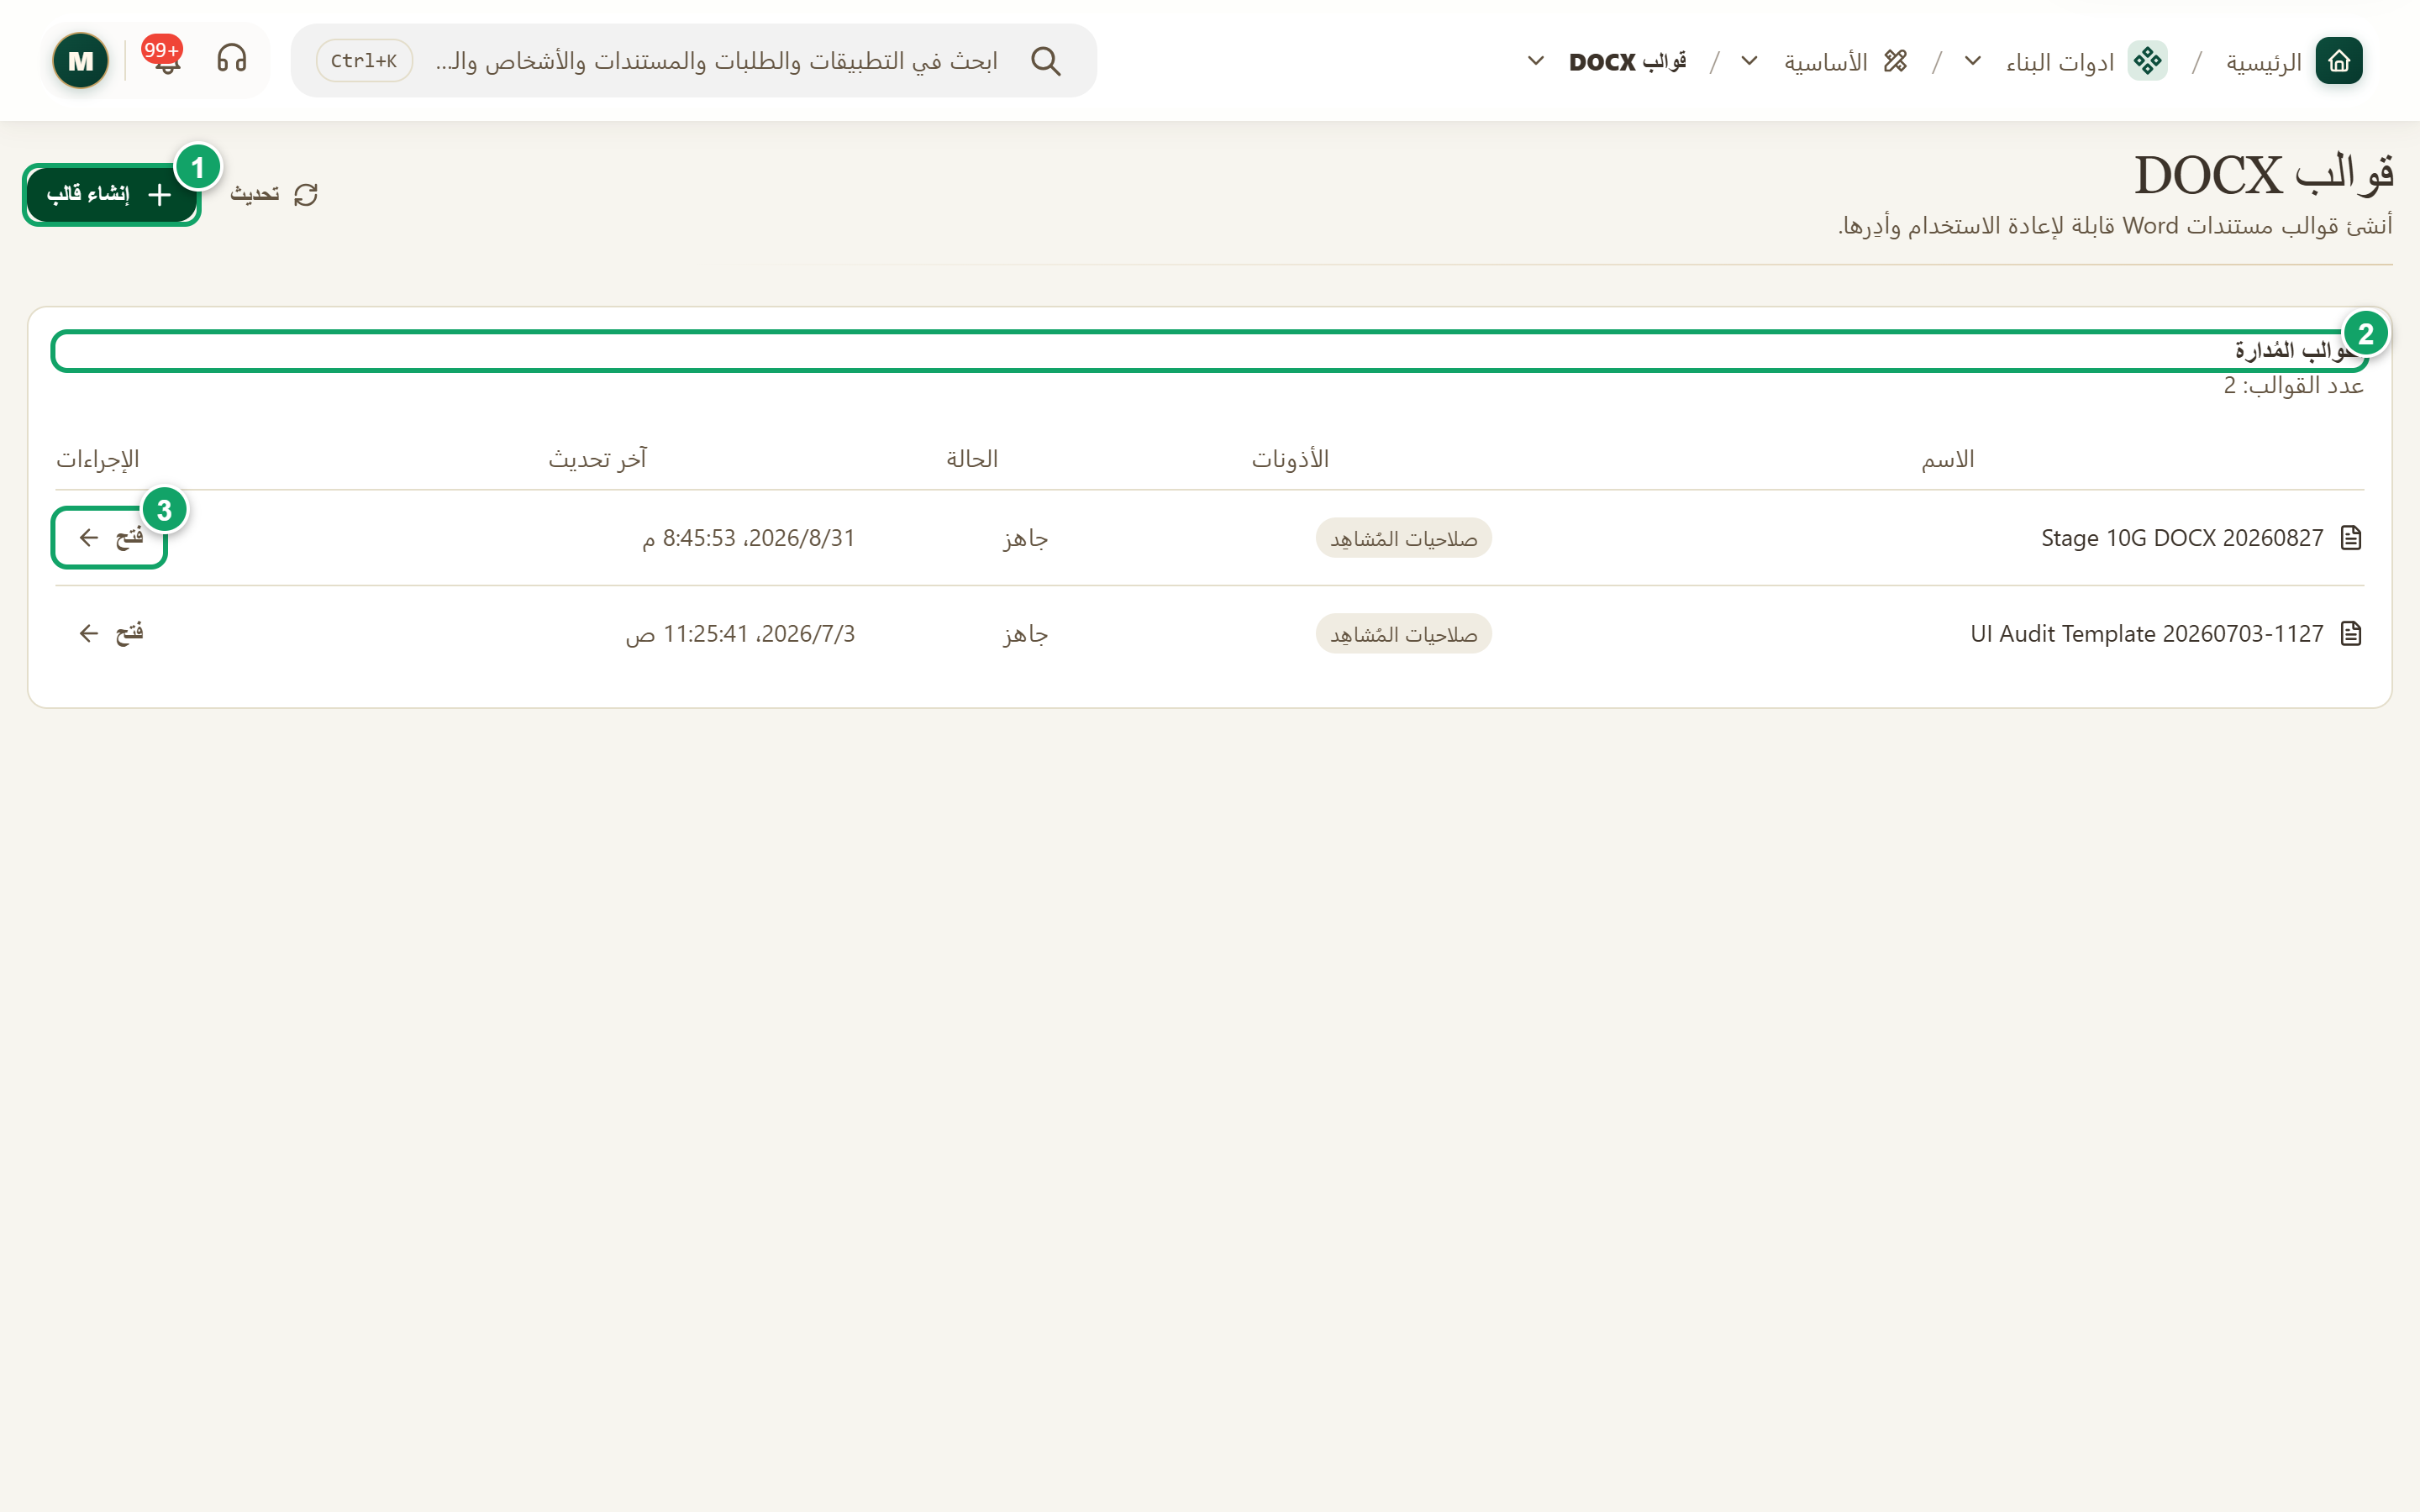
\includegraphics[width=0.95\linewidth,height=0.72\textheight,keepaspectratio]{figures/screens/ch06-docx-ar.png}
\caption{صفحة «قوالب DOCX»}
\label{fig:builder-docx-templates-screen}
\shotnote{تعرض الصفحة القوالب المُدارة وأذوناتها وحالاتها، وهي هنا قوالب اختبار. ① «إنشاء قالب»: يرفع ملف Word جديداً. ② «القوالب المُدارة»: القائمة مع حالة كل قالب. ③ «فتح»: يفتح القالب للإعدادات والإصدارات والاختبار.}
\end{figure}


\begin{table}[H]
\centering
\caption{ما الذي تجده هنا؟}
\label{tab:builder-docx-data}
\begin{tabularx}{\linewidth}{R{3.6cm} Y}
\rcHeaderRow
\thh{الجزء} & \thh{المحتوى والإجراء}\\
القوالب المُدارة & قائمة القوالب مع «الأذونات» و«الحالة»: «جاهز» عندما يوجد إصدار حالي، أو «يحتاج إلى مستند Word».\\
إنشاء قالب & ترفع «مستند Word» بصيغة \en{.docx} وحدها، وتكتب «اسم القالب» و«الوصف (اختياري)».\\
اسم الملف عند التنزيل & يقع في «الإعدادات الافتراضية المتقدمة»، ويُكتب تعبيراً يبني الاسم من بيانات السجل، مثل رقم الطلب. وإذا بقي فارغاً أو تعذّر حسابه، فيُستخدم اسم الملف المرفوع.\\
أذونات المستند & «صلاحيات المُشاهِد»، وهي الموصى بها، تعرض فقط ما يستطيع من ينزّل الملف رؤيته. أما «صلاحيات المسؤول» فقد تضع في المستند بيانات لا يراها.\\
إنشاء بمساعدة الذكاء الاصطناعي & زر يظهر عندما يكون «الذكاء الاصطناعي في أدوات البناء» مفعّلاً، فيبدأ القالب بمساعد يقترح مسودة تراجعها قبل حفظها.\\
\end{tabularx}
\end{table}

\begin{figure}[H]
\centering
\begin{tikzpicture}[node distance=0.5cm]
\node[stepBox] (a) {\RL{ملف Word بوسوم}};
\node[stepBox,below=of a] (b) {\RL{إنشاء قالب واختباره}};
\node[stepBox,below=of b] (c) {\RL{إجراء «قالب DOCX» في السجل}};
\node[stepBox,below=of c] (d) {\RL{المستخدم يضغط الزر}};
\draw[flowsTo] (a) -- (b);
\draw[flowsTo] (b) -- (c);
\draw[flowsTo] (c) -- (d);
\end{tikzpicture}
\rclegend
\caption{من ملف Word إلى مستند لكل سجل}
\label{fig:builder-docx-flow}
\shotnote{يبيّن المخطط أن القالب لا يرتبط بنوع سجلات بنفسه، بل يصل إلى المستخدم عبر إجراء من نوع «قالب DOCX» تضيفه في «الإجراءات والأتمتة». لذلك يأتي الاختبار على سجل حقيقي قبل الربط، لأن التحقق عند الرفع لا يكشف كل خطأ في موضع الوسوم.}
\end{figure}

\subsection{خطوات العمل والتحقق}
\begin{enumerate}
\item اكتب المستند في Word، وضع الوسوم بمفاتيح الحقول الفعلية، واجعل وسوم الشرط والتكرار في فقرة مستقلة.
\item افتح «قوالب DOCX» واضغط «إنشاء قالب»، ثم ارفع الملف واكتب الاسم واضغط «إنشاء قالب».
\item افتح «اختبار وتحميل»، واختر سجلاً، ثم «إنشاء وتنزيل» وراجع المستند.
\item أضف في نوع السجلات إجراءً من نوع «قالب DOCX» واختر القالب في «اختر القالب»، ثم انشر.
\end{enumerate}

\textbf{تحقق ومعالجة المشكلة:} يجب أن تظهر حالة القالب «جاهز»، وأن ينزّل زر الإجراء مستنداً ممتلئاً ببيانات السجل. فإذا ظهر «هذا المستند يحتاج إلى مراجعة» عند الرفع، فصحّح الوسوم المذكورة وأعد الرفع. وإذا ظهرت قيمة فارغة، فتأكد من أنك استخدمت مفتاح الحقل لا تسميته.

\clearpage
\section{وسوم قوالب DOCX والتكرار}
\label{sec:builder-feature-docx-tags}

الوسم نص بين قوسين مزدوجين تكتبه في ملف Word حيث يجب أن تظهر قيمة من السجل. ويقرأ كيان الوسوم عند إنشاء المستند ويستبدل بها البيانات، في متن المستند وفي رأس الصفحة وتذييلها والحواشي والتعليقات. وللوسوم ثلاثة أنواع: وسم قيمة يوضع داخل السطر مع نص آخر، ووسوم تحكم للشرط والتكرار تشغل فقرة كاملة أو صفاً كاملاً من جدول، ووسوم إضافية تُدرج صورة أو رابطاً أو رمز QR أو فاصل صفحة.

\textbf{المسار ومن يستخدمه:} تُكتب الوسوم في Word قبل رفع الملف من «ادوات البناء» ← «الأساسية» ← «قوالب DOCX». يكتبها من يدير القوالب، ويستعمل فيها مفاتيح الحقول كما تظهر في نوع السجلات.

\begin{rcnote}[مثال: شركة الأفق]
يكتب مسؤول النظام في خطاب تأكيد الزيارة سطر «موعد الزيارة:» ثم الوسم \en{\{\{ \$record.visit\_date \}\}}. ويضع حول هذا السطر فقرة شرط مستقلة، فإن لم يُحدَّد الموعد بعد ظهرت بدلاً منه جملة «سيُرسل الموعد بعد المراجعة».
\end{rcnote}

\begin{table}[H]
\centering
\caption{الوسوم وأماكنها في Word}
\label{tab:builder-docx-tags}
\begin{tabularx}{\linewidth}{R{3.6cm} Y}
\rcHeaderRow
\thh{الوسم} & \thh{ماذا يفعل؟ وأين يوضع؟}\\
\en{\{\{ \$record.field\_key \}\}} & يضع قيمة حقل بمفتاحه لا بتسميته، ويمكن أن يشارك فقرة فيها نص آخر. والقيمة الفارغة تُطبع نصاً فارغاً.\\
\en{\{\{\#if ...\}\}} و\en{\{\{else\}\}} و\en{\{\{/if\}\}} & تُظهر الفقرات التي بينها عندما يتحقق الشرط، وإلا تُظهر ما بعد \en{else}. وكل وسم منها وحده في فقرته أو صفه.\\
\en{\{\{\#each list as item\}\}} و\en{\{\{/each\}\}} & تكرر الفقرات أو صفوف الجدول التي بينها لكل عنصر. وداخلها \en{\$index} الذي يبدأ من الصفر، و\en{\$first} و\en{\$last}.\\
\en{\{\{@image ... width=120\}\}} & يُدرج صورة PNG أو JPEG أو WebP حتى 10 ميغابايت، ويُضاف \en{optional=true} حين يجوز غيابها.\\
\en{\{\{@link url label\}\}} & يُدرج رابطاً يبدأ بـ \en{http} أو \en{https} أو \en{mailto} فقط.\\
\en{\{\{@qr ... width=120\}\}} & يُنشئ رمز QR من قيمة غير فارغة، مثل رقم الطلب.\\
\en{\{\{@pageBreak\}\}} & يبدأ صفحة جديدة.\\
\en{\{\{> ...\}\}} & يُدرج متن قالب آخر، مثل بند ثابت، ويوضع وحده في فقرته. ويُسمح بخمسة مستويات إدراج متداخلة.\\
\end{tabularx}
\end{table}

\begin{table}[H]
\centering
\caption{البيانات التي يقرأ منها القالب}
\label{tab:builder-docx-tags-context}
\begin{tabularx}{\linewidth}{R{3.6cm} Y}
\rcHeaderRow
\thh{الجذر} & \thh{ما يحتويه}\\
\en{\$record} & حقول السجل المختار وبياناته العامة بمفاتيحها.\\
\en{\$inverseRelations} & السجلات التي تشير إلى هذا السجل، كما ضُبطت في الإجراء.\\
\en{\$organization} و\en{\$member} & المؤسسة الحالية والعضو الذي يُنشئ المستند.\\
\en{\$now} & وقت إنشاء المستند، وتنسّقه بنفسك.\\
\en{getRecords} & دالة تجلب سجلات من نوع آخر بحد أقصى 500 سجل في كل استدعاء، وتخضع لصلاحيات من ينزّل المستند ما لم يُضبط القالب على «صلاحيات المسؤول».\\
\end{tabularx}
\end{table}

\begin{rcwarn}[التحقق عند الرفع لا يضمن موضع الوسوم]
يكتشف التحقق الوسوم الفارغة أو غير المغلقة والأوامر غير المدعومة، مثل \en{@html} و\en{@chart} وإدراج XML الخام. لكنه لا يضمن أن وسم الشرط أو التكرار يشغل فقرته وحده، فقد ينجح الرفع ثم يختفي النص أو يُطبع الوسم. لذلك اختبر كل شرط وتكرار على سجل حقيقي بعد كل تعديل.
\end{rcwarn}

\begin{figure}[H]
\centering
\begin{tikzpicture}[node distance=0.5cm]
\node[stepBox] (a) {\RL{وسوم القيم داخل السطر}};
\node[stepBox,below=of a] (b) {\RL{وسوم الشرط والتكرار}\\\RL{في فقرات مستقلة}};
\node[stepBox,below=of b] (c) {\RL{الرفع والتحقق}};
\node[stepBox,below=of c] (d) {\RL{الاختبار على سجل حقيقي}};
\draw[flowsTo] (a) -- (b);
\draw[flowsTo] (b) -- (c);
\draw[flowsTo] (c) -- (d);
\end{tikzpicture}
\rclegend
\caption{ترتيب كتابة الوسوم واختبارها}
\label{fig:builder-docx-tags-flow}
\shotnote{يفصل المخطط بين وسوم القيم التي تعيش داخل الجملة ووسوم التحكم التي تحتاج إلى فقرة أو صف كامل، لأن الخلط بينهما أكثر أسباب الأخطاء شيوعاً. وينتهي بالاختبار على سجل حقيقي، فهو وحده يثبت أن الشرط والتكرار يعملان كما تريد.}
\end{figure}

\subsection{خطوات العمل والتحقق}
\begin{enumerate}
\item اكتب في Word كل وسم قيمة بمفتاح الحقل، مثل \en{\{\{ \$record.field\_key \}\}}، داخل الجملة التي يخصها.
\item ضع وسم بداية الشرط أو التكرار في فقرة مستقلة، ثم الفقرات أو صف الجدول الذي يتكرر، ثم وسم النهاية في فقرة مستقلة.
\item أضف الصور والروابط ورموز QR بالوسوم المخصصة لها، واكتب خياراتها دون مسافات داخل القيم.
\item ارفع الملف، فإذا ظهر «هذا المستند يحتاج إلى مراجعة» فصحّح المشكلات المذكورة وأعد الرفع.
\item اختبر القالب على سجل ممتلئ وآخر تنقصه بعض القيم، وعلى قائمة فارغة وأخرى فيها عدة عناصر.
\end{enumerate}

\textbf{تحقق ومعالجة المشكلة:} يجب أن تُستبدل كل الوسوم بقيم، وأن تختفي وسوم التحكم من الملف الناتج. فإذا طُبع وسم شرط أو اختفى نص حوله، فانقل الوسم إلى فقرة مستقلة. وإذا لم يتكرر أي صف، فتأكد من أن التعبير يُرجع قائمة، ومن أن الاسم المستعار بعد \en{as} مكتوب كما تستخدمه داخل الحلقة.

\clearpage
\section{مساحة عمل قالب DOCX ومساعد الذكاء الاصطناعي}
\label{sec:builder-feature-docx-workspace}

عندما تضغط «فتح» بجانب قالب تنتقل إلى مساحة عمله، وفيها ثلاثة تبويبات: «الإعدادات» و«الإصدارات» و«اختبار وتحميل». وتعرض شارة في رأسها «جاهز للاستخدام» إذا كان للقالب إصدار حالي، أو «يتطلب إصدار DOCX». ومن هنا تعدّل القالب وتستبدل ملفه وتجرّبه قبل أن يصل إلى المستخدمين. وإذا كان «الذكاء الاصطناعي في أدوات البناء» مفعّلاً، فيمكنك أن تطلب من المساعد تعديل القالب، فيقترح مسودة لا تُحفظ إلا بعد مراجعتك.

\textbf{المسار ومن يستخدمه:} «ادوات البناء» ← «الأساسية» ← «قوالب DOCX» ← «فتح». يستخدمها من يدير القوالب كلما عدّل نص المستند أو أراد تجربته.

\begin{rcnote}[مثال: شركة الأفق]
يختبر مسؤول النظام خطاب تأكيد الزيارة على الطلب HZN-VR-0001 بصيغة PDF. ثم يفتح «الإصدارات» ويطلب من المساعد أن يجعل التحية أكثر رسمية، ويراجع المسودة قبل اعتمادها. فيختبر من ①، ثم يفتح ② ويبدأ المساعد من ④.
\end{rcnote}

\begin{figure}[H]
\centering
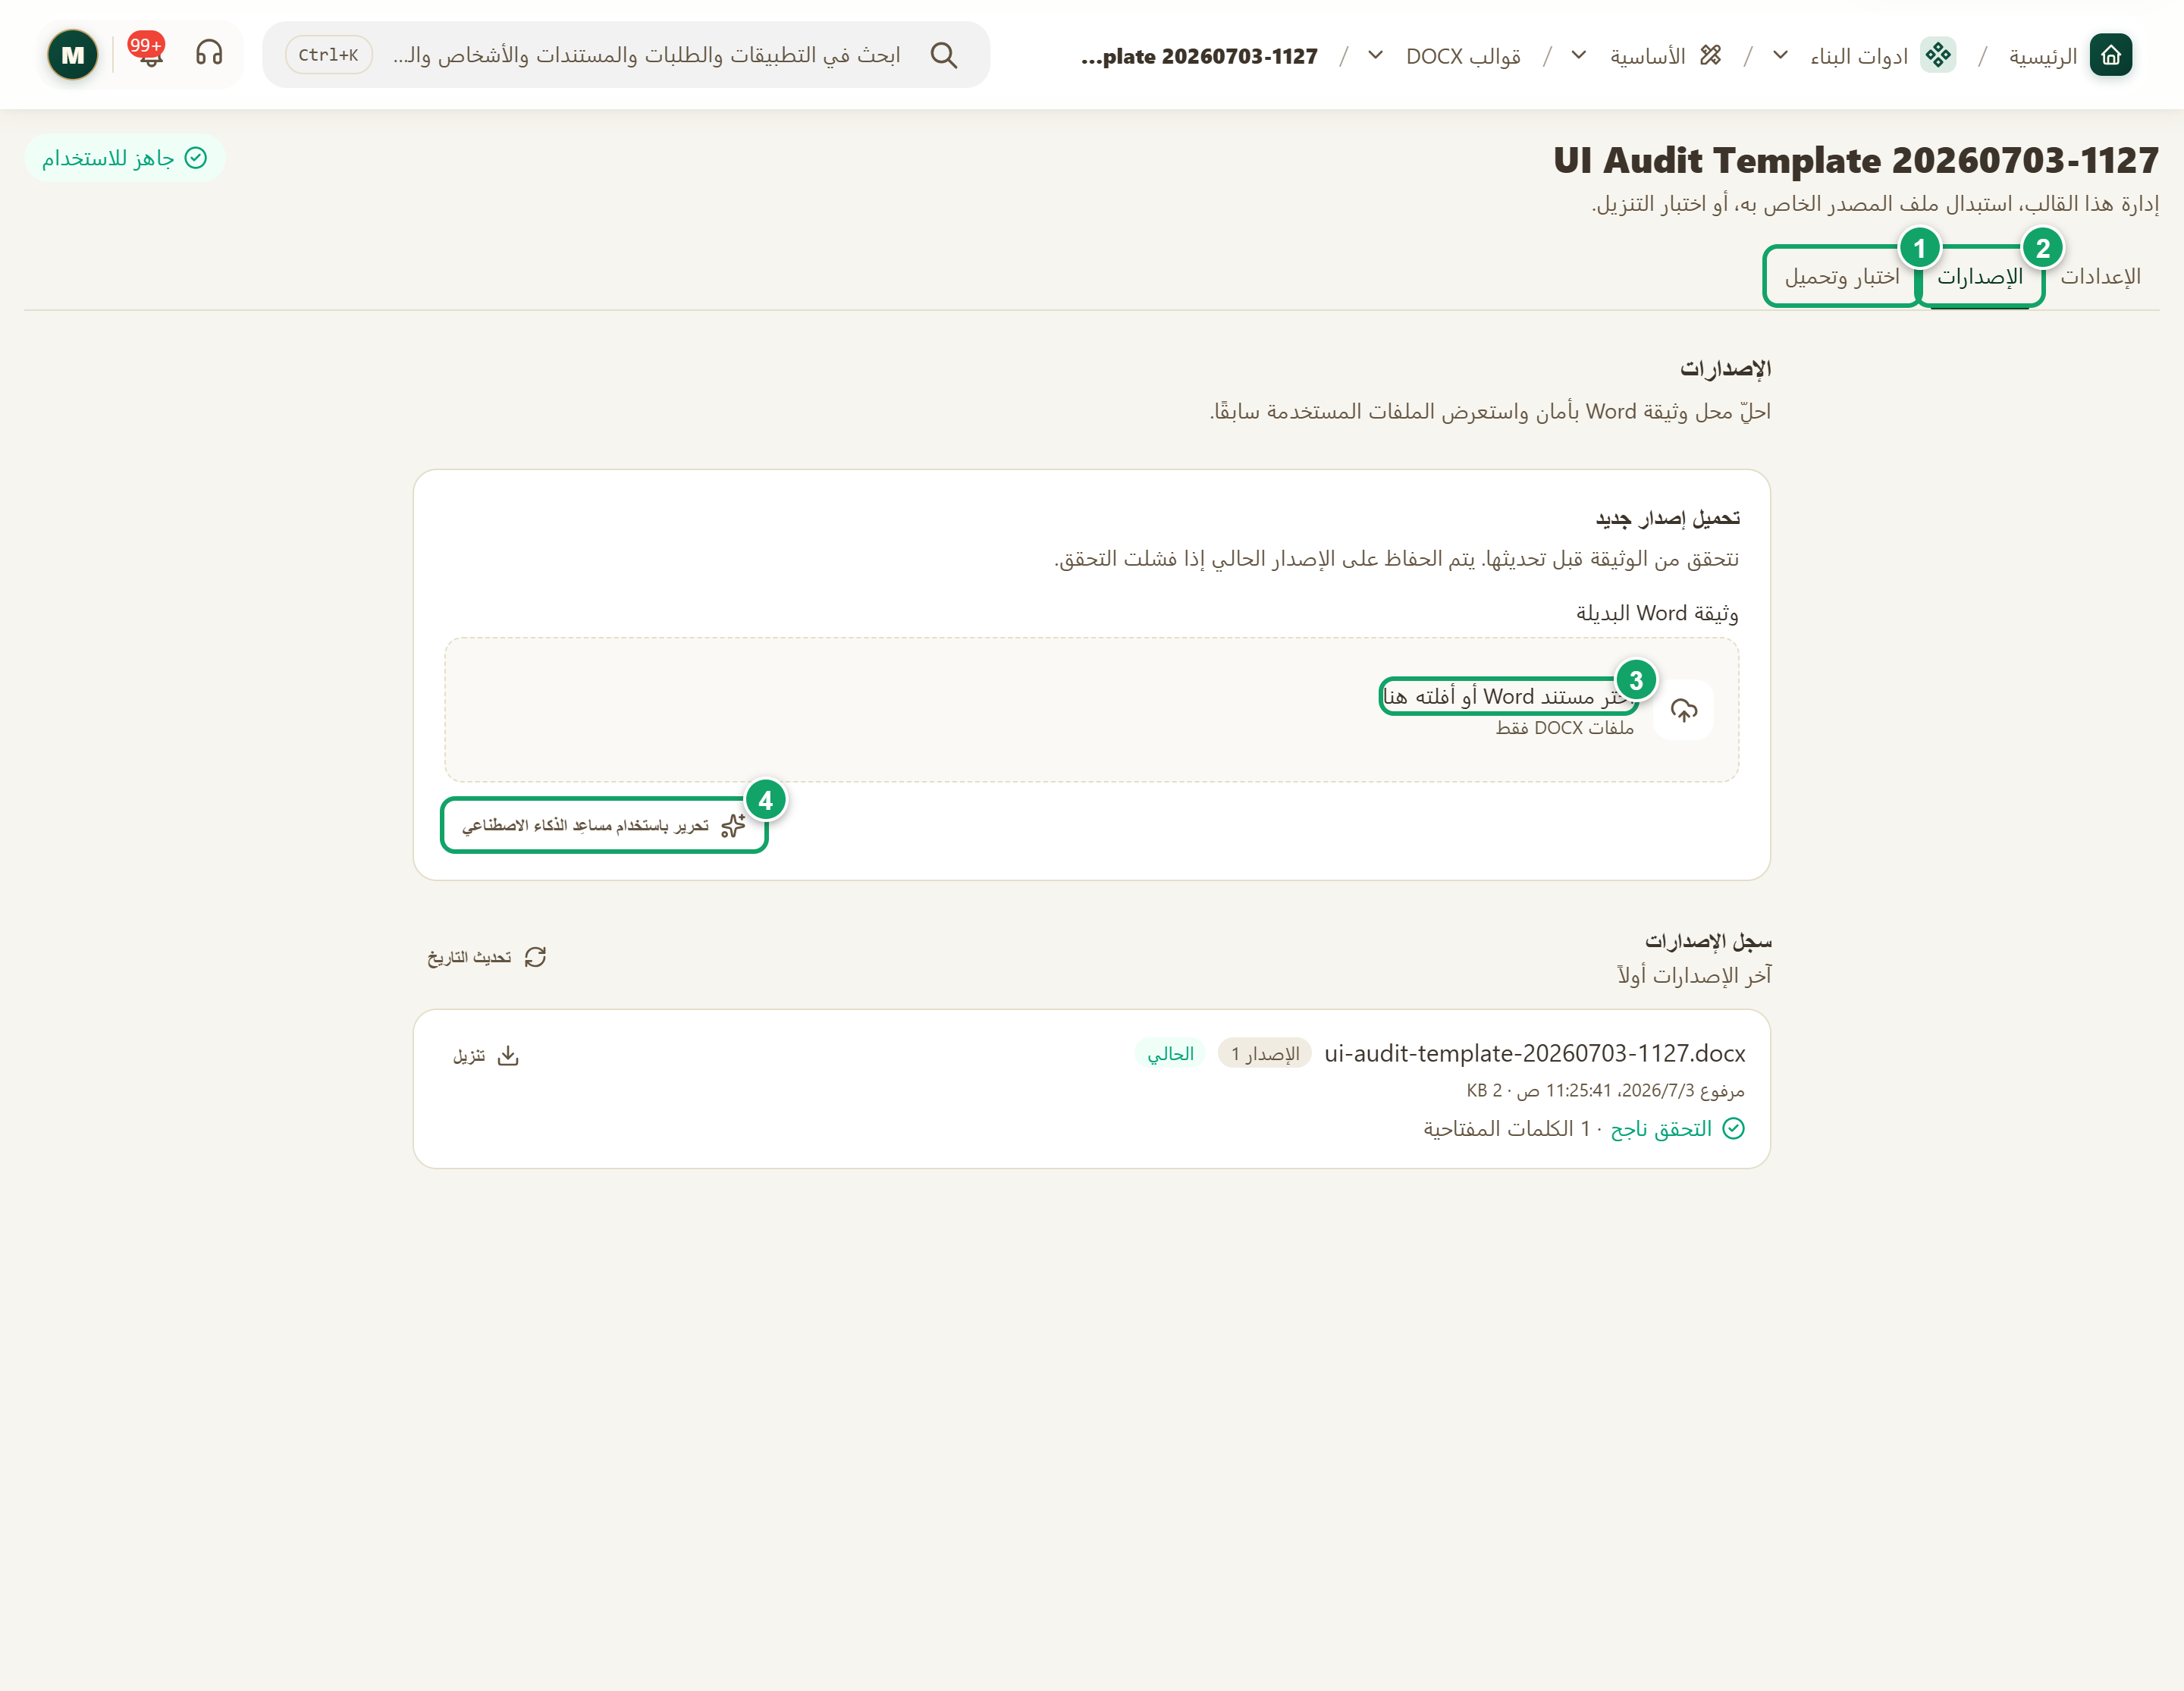
\includegraphics[width=0.95\linewidth,height=0.72\textheight,keepaspectratio]{figures/screens/ch06-docx-workspace-ar.png}
\caption{تبويب «الإصدارات» في مساحة عمل قالب DOCX}
\label{fig:builder-docx-workspace-screen}
\shotnote{تعرض الصورة قالب DOCX اختبارياً في test2 مفتوحاً على تبويب «الإصدارات»، وتحته «سجل الإصدارات» الذي يبيّن الإصدار الحالي ونتيجة التحقق منه. وتجمع هذه الشاشة طريقتي إنشاء إصدار جديد: رفع ملف بديل، أو طلب مسودة من المساعد، ولذلك يسبقهما الاختبار. ① «اختبار وتحميل»: تجرّب فيه القالب على سجل قبل أي تعديل. ② «الإصدارات»: التبويب المعروض. ③ «اختر مستند Word أو أفلته هنا»: تختار منه ملف الإصدار البديل. ④ «تحرير باستخدام مساعِد الذكاء الاصطناعي»: يفتح صفحة المساعد لاختيار السياق وكتابة الطلب.}
\end{figure}

\begin{table}[H]
\centering
\caption{تبويبات مساحة العمل}
\label{tab:builder-docx-workspace-tabs}
\begin{tabularx}{\linewidth}{R{3.6cm} Y}
\rcHeaderRow
\thh{التبويب} & \thh{المحتوى والإجراء}\\
الإعدادات & «اسم القالب» و«الوصف (اختياري)» واسم الملف عند التنزيل و«أذونات المستند»، ثم «حفظ التغييرات».\\
الإصدارات & تختار ملف Word بديلاً وتضغط زر التحقق والرفع، فيتحقق كيان من الملف قبل أن يجعله الإصدار الحالي. ويعرض «سجل الإصدارات» الإصدارات من الأحدث، مع علامة «الحالي» ونتيجة التحقق وزر «تنزيل».\\
اختبار وتحميل & تختار بيانات الاختبار: «استخدم سجلاً» أو «لصق JSON — متقدم»، ثم الصيغة Word أو PDF. وتغيّر «خيارات متقدمة» اسم الملف والأذونات لهذا التنزيل فقط، ثم تضغط «إنشاء وتنزيل».\\
\end{tabularx}
\end{table}

\begin{table}[H]
\centering
\caption{مساعد DOCX بالذكاء الاصطناعي}
\label{tab:builder-docx-workspace-ai}
\begin{tabularx}{\linewidth}{R{3.6cm} Y}
\rcHeaderRow
\thh{المرحلة} & \thh{ما يحدث فيها}\\
البدء & من «إنشاء بمساعدة الذكاء الاصطناعي» عند إنشاء قالب، أو «تحرير باستخدام مساعِد الذكاء الاصطناعي» في «الإصدارات» لتعديل الإصدار الحالي.\\
السياق & تختار «استخدم سياق الكيان» مع سجل اختياري، فإن لم تختر سجلاً استُخدمت بيانات عينة. أو تختار «JSON يدوي» في حدود 256 كيلوبايت.\\
الموافقة على الإرسال & تؤكد أن نص المستند والسياق وتعليماتك سترسل إلى مزود الذكاء الاصطناعي الذي ضبطته المؤسسة. أما ملف Word نفسه فلا يُرسل.\\
المراجعة & كل طلب ينشئ مراجعة مرقّمة، فتقرأ «ملخص التغيير» و«رموز القالب»، وتعرض معاينة أو تضغط «تنزيل DOCX». ويجب أن تحل كل سؤال في «أسئلة لحلها» قبل الاعتماد.\\
الاعتماد أو الحذف & زر الموافقة والحفظ ينشئ إصداراً جديداً دون تغيير إعدادات القالب أو الإجراءات المرتبطة به، و«حذف المسودة» يلغيها. وتنتهي المسودة بعد 24 ساعة دون نشاط، وبعد سبعة أيام على الأكثر.\\
\end{tabularx}
\end{table}

\begin{rcwarn}[الإصدار الجديد يعمل فوراً]
تستخدم أزرار الإجراءات في السجلات الإصدار الحالي دائماً، لذلك يصل أي إصدار ترفعه أو تعتمده إلى المستخدمين مباشرة. فاختبر الملف على سجل حقيقي قبل رفعه، واحتفظ بنسخة من الملف المعتمد خارج كيان.
\end{rcwarn}

\begin{figure}[H]
\centering
\begin{tikzpicture}[node distance=0.5cm]
\node[stepBox] (a) {\RL{فتح القالب}};
\node[stepBox,below=of a] (b) {\RL{اختبار وتحميل على سجل}};
\node[stepBox,below=of b] (c) {\RL{إصدار جديد: رفع ملف}\\\RL{أو مسودة من المساعد}};
\node[stepBox,below=of c] (d) {\RL{المراجعة والاختبار}};
\node[stepBox,below=of d] (e) {\RL{يصبح الإصدار الحالي}};
\draw[flowsTo] (a) -- (b);
\draw[flowsTo] (b) -- (c);
\draw[flowsTo] (c) -- (d);
\draw[flowsTo] (d) -- (e);
\end{tikzpicture}
\rclegend
\caption{تعديل قالب DOCX بأمان}
\label{fig:builder-docx-workspace-flow}
\shotnote{يجمع المخطط طريقتي إنشاء إصدار جديد: رفع ملف بديل، أو اعتماد مسودة اقترحها المساعد. وفي الطريقتين تأتي المراجعة قبل أن يصبح الإصدار حالياً، لأن الإجراءات في السجلات تستخدمه منذ تلك اللحظة.}
\end{figure}

\subsection{خطوات العمل والتحقق}
\begin{enumerate}
\item افتح القالب، ثم افتح «اختبار وتحميل» واختر «استخدم سجلاً» وحدد سجلاً حقيقياً.
\item اختر الصيغة، واضغط «إنشاء وتنزيل»، وراجع الملف الناتج.
\item لتعديل النص يدوياً، افتح «الإصدارات» واختر ملف Word البديل، ثم اضغط زر التحقق والرفع.
\item لتعديله بالمساعد، اضغط «تحرير باستخدام مساعِد الذكاء الاصطناعي»، واختر السياق، واكتب طلباً واحداً محدداً في «تعليمات»، ثم أكّد موافقتك على الإرسال واضغط «ابدأ مساعداً ذكياً». أما الطلبات اللاحقة فترسلها بزر «إنشاء مسودة».
\item راجع «ملخص التغيير» والمعاينة، وحل الأسئلة المفتوحة، ثم اضغط زر الموافقة والحفظ.
\end{enumerate}

\textbf{تحقق ومعالجة المشكلة:} يجب أن تظهر رسالة «إصدار جديد للقالب جاهز للاستخدام.» وأن يحمل الإصدار الجديد علامة «الحالي» في «سجل الإصدارات». فإذا ظهر «لم يتم تحميل هذا المستند»، فاضغط «عرض المشكلات» وصحّح الملف، ويبقى الإصدار السابق نشطاً حتى ذلك الحين. وإذا لم يظهر زر المساعد، فاطلب من مسؤول المؤسسة تفعيل «الذكاء الاصطناعي في أدوات البناء».

\clearpage
\section{قوالب XLSX}
\label{sec:builder-feature-xlsx-templates}

قالب XLSX مصنف Excel فيه وسوم بالطريقة نفسها، يملؤه كيان من بيانات السجل وينزّله بصيغة Excel أو PDF. ويناسب الكشوف والتقارير الجدولية التي تتكرر صفوفها، لأن الوسوم تستطيع تكرار الصفوف والأعمدة. ويحافظ الوسم الموضوع وحده في خلية على نوع القيمة رقماً أو تاريخاً.

\textbf{المسار ومن يستخدمه:} «ادوات البناء» ← «الأساسية» ← «قوالب XLSX». يديرها من يملك إدارة أدوات البناء.

\begin{rcnote}[مثال: شركة الأفق]
يجهّز مسؤول النظام مصنف «كشف زيارات الفرع» يكرر صفاً لكل زيارة، ويربطه بزر إجراء من نوع «قالب XLSX»، فتنزّل سارة الخطيب الكشف جاهزاً بصيغة Excel. ويرفع المصنف من ①.
\end{rcnote}

\begin{figure}[H]
\centering
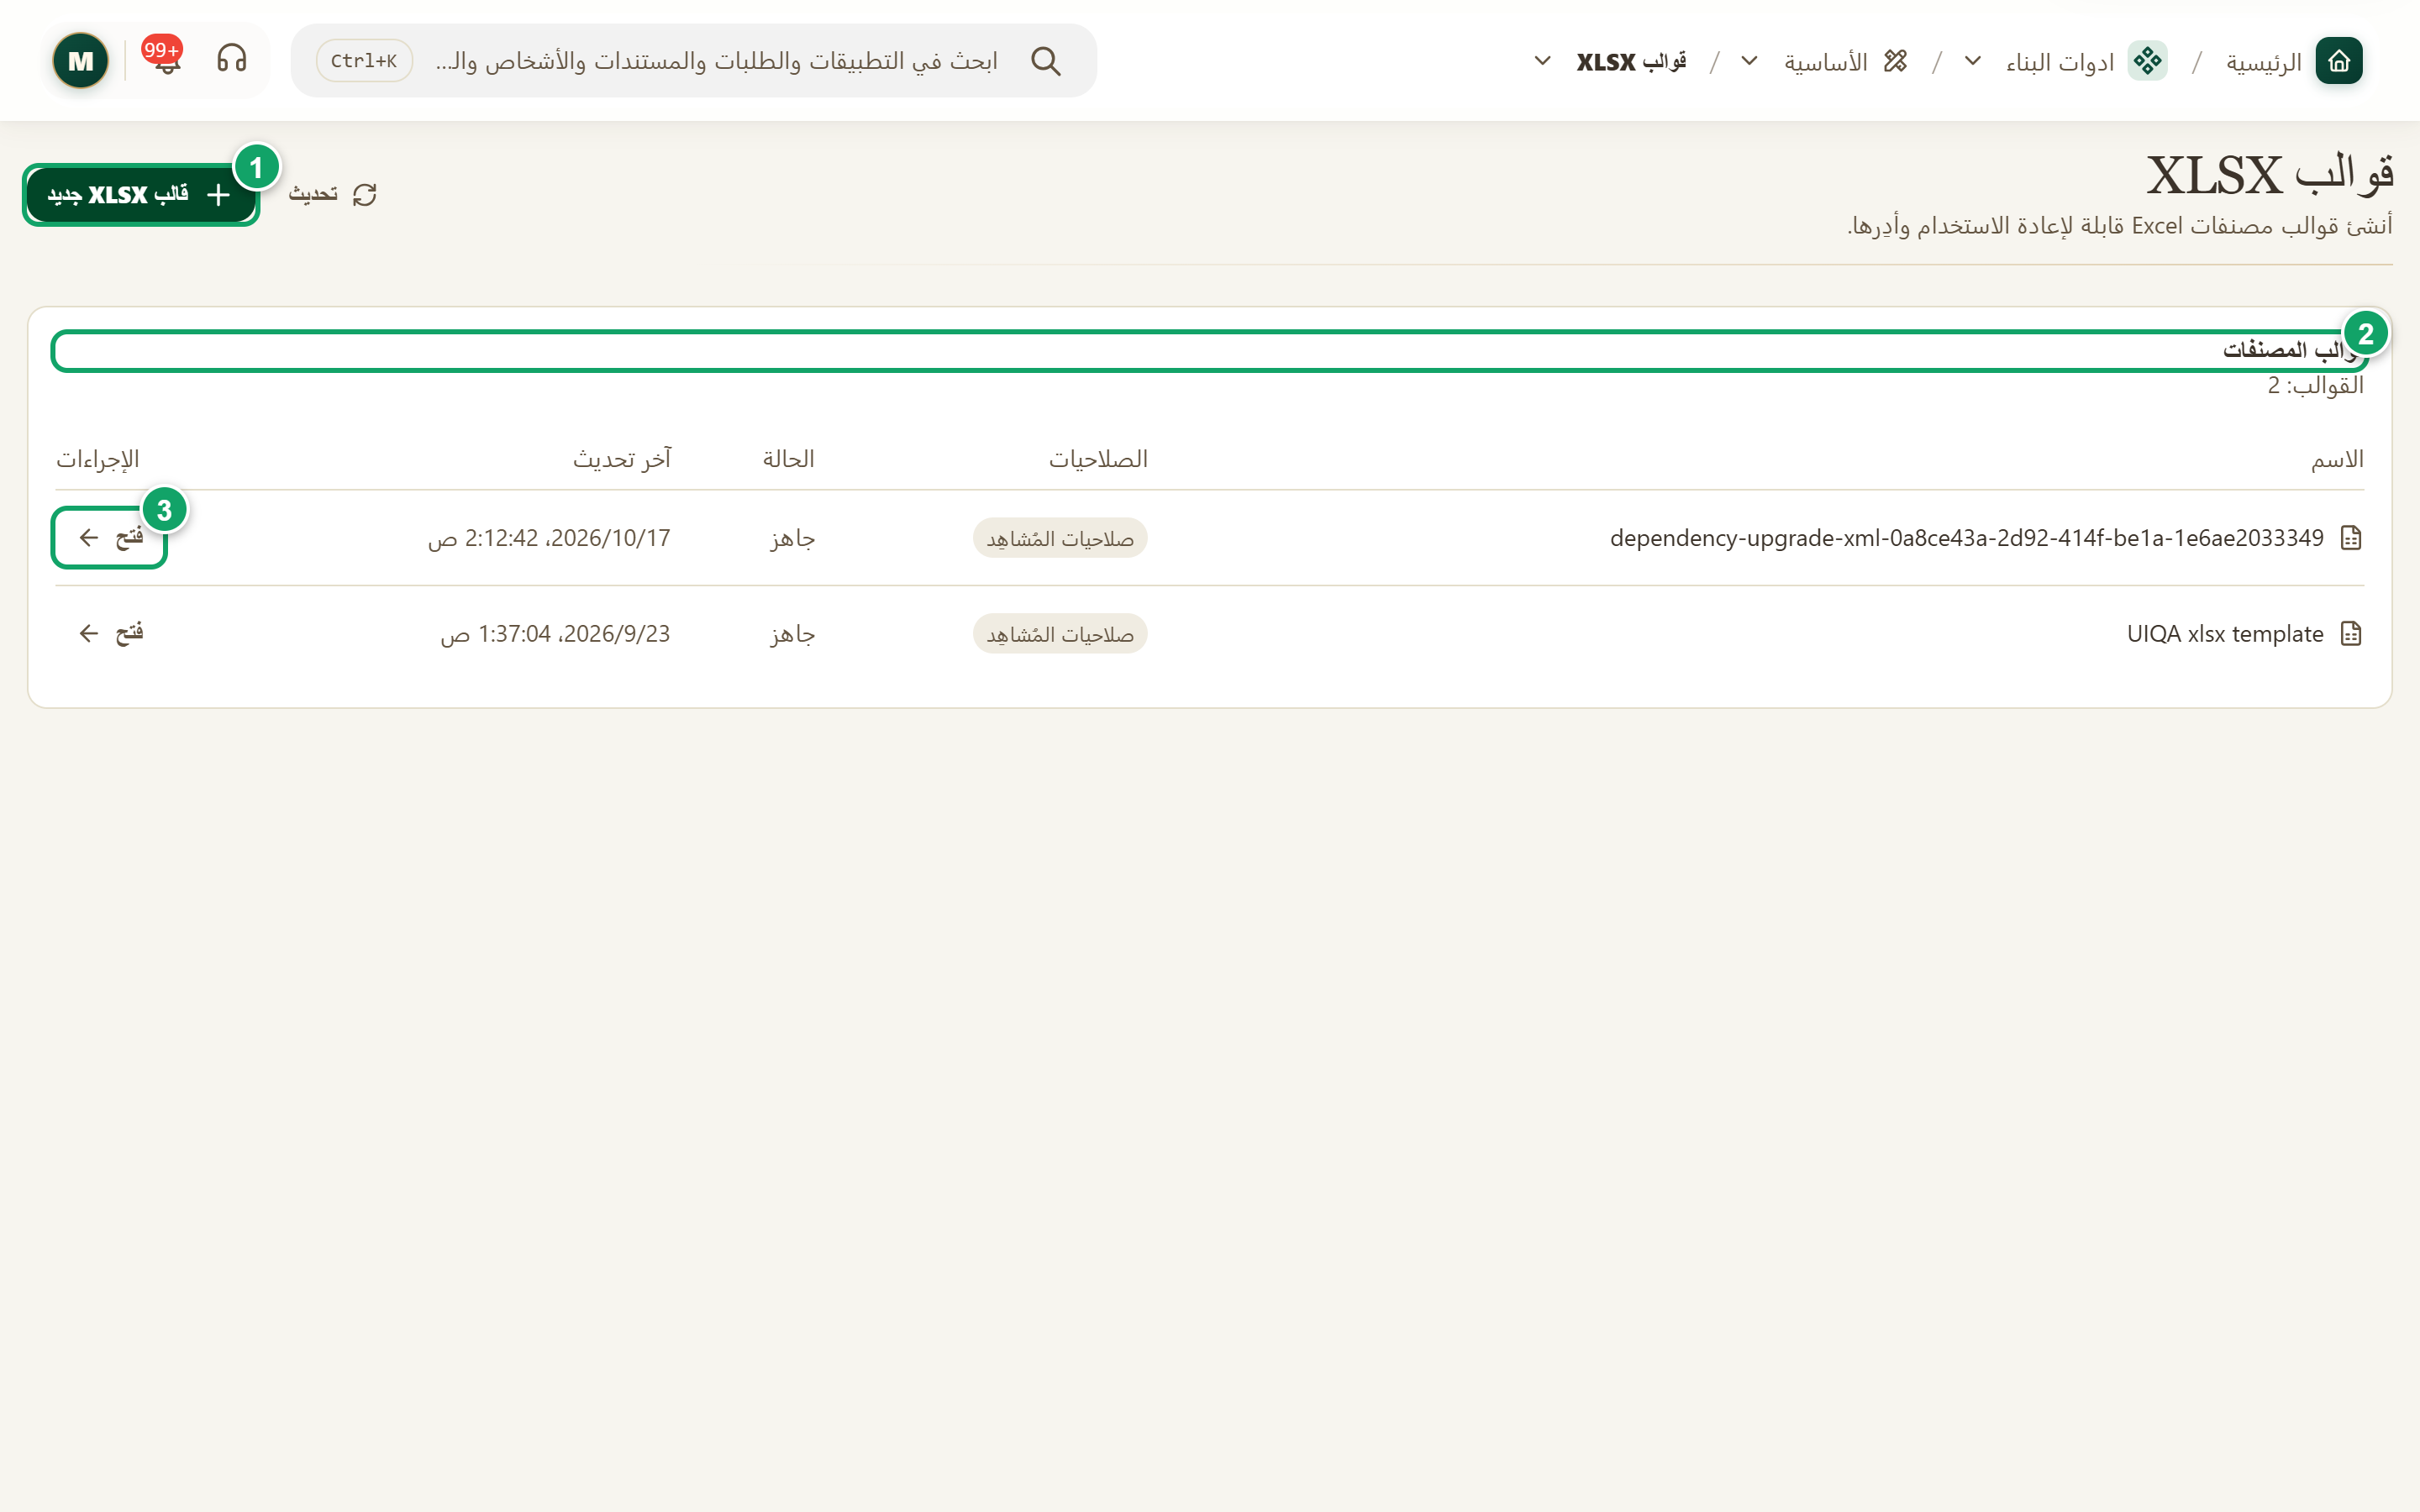
\includegraphics[width=0.95\linewidth,height=0.72\textheight,keepaspectratio]{figures/screens/ch06-xlsx-ar.png}
\caption{صفحة «قوالب XLSX»}
\label{fig:builder-xlsx-templates-screen}
\shotnote{تعرض الصفحة قوالب المصنفات وحالاتها، وهي هنا قوالب اختبار. ① «قالب XLSX جديد»: يرفع مصنف Excel. ② «قوالب المصنفات»: القائمة مع الحالة. ③ «فتح»: يفتح القالب لاختباره.}
\end{figure}


\begin{table}[H]
\centering
\caption{ما الذي تجده هنا؟}
\label{tab:builder-xlsx-data}
\begin{tabularx}{\linewidth}{R{3.6cm} Y}
\rcHeaderRow
\thh{الجزء} & \thh{المحتوى والإجراء}\\
قوالب المصنفات & قائمة القوالب وحالتها: «جاهز» أو «يحتاج إلى مصنف Excel».\\
قالب XLSX جديد & ترفع «مصنف Excel» وتكتب «اسم القالب»، ويمكنك ضبط «صيغة اسم الملف عند التنزيل» و«أذونات البيانات».\\
التحقق عند الرفع & يرفض كيان المصنفات التي فيها وحدات ماكرو أو كائنات مضمّنة أو روابط إلى مصنفات خارجية، ويعرض المشكلات تحت «هذا المصنف يحتاج إلى مراجعة».\\
الإصدارات & استبدال المصنف بإصدار جديد ومراجعة الإصدارات السابقة.\\
اختبار وتحميل & تجربة القالب ببيانات، ثم «إنشاء XLSX» أو «إنشاء PDF».\\
\end{tabularx}
\end{table}

\begin{figure}[H]
\centering
\begin{tikzpicture}[node distance=0.5cm]
\node[entity] (tpl) {\RL{قالب XLSX}};
\node[entityOpt,below right=0.7cm and 0.3cm of tpl] (xlsx) {\RL{ملف Excel}};
\node[entityOpt,below left=0.7cm and 0.3cm of tpl] (pdf) {\RL{ملف PDF}};
\draw[dependsOnOpt] (tpl.south) -- ++(0,-0.3) -| (xlsx.north);
\draw[dependsOnOpt] (tpl.south) -- ++(0,-0.3) -| (pdf.north);
\end{tikzpicture}
\rclegend
\caption{صيغتا الإخراج}
\label{fig:builder-xlsx-outputs}
\shotnote{يوضّح الشكل أن القالب الواحد يُخرج ملف Excel أو PDF، وتختار ما يُسمح به عند ربطه بالإجراء عبر «السماح بملفات PDF». فاستخدم Excel عندما يحتاج المستلم إلى معالجة الأرقام، وPDF عندما تريد نسخة ثابتة للعرض أو الأرشيف.}
\end{figure}

\subsection{خطوات العمل والتحقق}
\begin{enumerate}
\item جهّز المصنف في Excel، وضع الوسوم في الخلايا المناسبة.
\item افتح «قوالب XLSX» واضغط «قالب XLSX جديد»، ثم ارفع المصنف واكتب الاسم واضغط «إنشاء قالب».
\item جرّب القالب من «اختبار وتحميل»، ثم أضف إجراءً من نوع «قالب XLSX» في نوع السجلات واختر القالب.
\end{enumerate}

\textbf{تحقق ومعالجة المشكلة:} يجب أن تظهر حالة القالب «جاهز»، وأن يتكرر الصف لكل عنصر في الملف الناتج. فإذا ظهر رقم نصاً، فاجعل الوسم وحده في خليته. وإذا تعذّر عليك إنشاء القالب، فإدارة القوالب تحتاج إلى صلاحية إدارة أدوات البناء لا إلى مقعد كامل فقط.

\clearpage
\section{وسوم قوالب XLSX والطباعة}
\label{sec:builder-feature-xlsx-tags}

تُكتب وسوم المصنف في الخلايا العادية، والفرق الأهم عن Word هو الاتجاه: وسم \en{each} يكرر الصفوف إلى الأسفل، ووسم \en{eachCol} يكرر الأعمدة إلى الجانب. وعندما يتقاطع تكرار صفوف مع تكرار أعمدة ينتج جدول كامل، فيه صف لكل عنصر من القائمة الأولى وعمود لكل عنصر من الثانية. ويحافظ كيان على الصيغ والتنسيق والمخططات وإعدادات الطباعة الموجودة في المصنف، ويعدّل مراجعها عندما تتوسع الصفوف والأعمدة.

\textbf{المسار ومن يستخدمه:} تُكتب الوسوم في Excel قبل رفع المصنف من «ادوات البناء» ← «الأساسية» ← «قوالب XLSX». يكتبها من يدير القوالب.

\begin{rcnote}[مثال: شركة الأفق]
يضع مسؤول النظام في «كشف زيارات الفرع» تكرار صفوف لكل فرع وتكرار أعمدة لكل شهر. فيظهر في الملف الناتج صف للمقر الرئيسي في دمشق وآخر لفرع حلب، وفي كل خلية عدد زيارات الفرع في ذلك الشهر.
\end{rcnote}

\begin{table}[H]
\centering
\caption{وسوم الخلايا والتكرار}
\label{tab:builder-xlsx-tags-loops}
\begin{tabularx}{\linewidth}{R{3.6cm} Y}
\rcHeaderRow
\thh{الوسم} & \thh{ماذا يفعل؟ وأين يوضع؟}\\
\en{\{\{ \$record.field\_key \}\}} & إذا كان وحده في الخلية بقي رقماً أو قيمة منطقية أو خلية فارغة، وإذا جاء مع نص آخر صار نصاً. والنص الذي يبدأ بـ \en{=} أو \en{+} أو \en{-} أو \en{@} يبقى نصاً ولا يتحول إلى صيغة.\\
\en{\{\{\#each list as item\}\}} و\en{\{\{/each\}\}} & يكرران صفوف المتن التي بينهما. ويوضع كل منهما في صف مستقل لا يحتوي أي خلية أخرى غير فارغة.\\
\en{\{\{\#if ...\}\}} و\en{\{\{else\}\}} و\en{\{\{/if\}\}} & تختار صفوفاً حسب شرط، ويوضع كل منها في صف مستقل بالطريقة نفسها.\\
\en{\{\{\#eachCol list as item\}\}} و\en{\{\{/eachCol\}\}} & يكرران الأعمدة التي بينهما. ويوضع كل منهما في عمود مستقل لا يحتوي أي خلية أخرى غير فارغة.\\
\en{\{\{\#ifCol ...\}\}} و\en{\{\{elseCol\}\}} و\en{\{\{/ifCol\}\}} & تختار أعمدة حسب شرط، ويوضع كل منها في عمود علامة مستقل.\\
\end{tabularx}
\end{table}

\begin{table}[H]
\centering
\caption{التوجيهات والصيغ والطباعة}
\label{tab:builder-xlsx-tags-directives}
\begin{tabularx}{\linewidth}{R{3.6cm} Y}
\rcHeaderRow
\thh{العنصر} & \thh{ما يجب أن تعرفه}\\
\en{\{\{@hideRow ...\}\}} و\en{\{\{@hideColumn ...\}\}} & يخفيان الصف أو العمود الناتج عندما يكون التعبير صحيحاً.\\
\en{\{\{@link url label\}\}} & رابط آمن يبدأ بـ \en{http} أو \en{https} أو \en{mailto}.\\
\en{\{\{@image ... width=120\}\}} و\en{\{\{@qr ... width=120\}\}} & صورة أو رمز QR يشغل خلية كاملة، ويتحرك مع الصفوف والأعمدة المتوسعة.\\
الصيغ & تبقى الصيغ كما هي، وتتعدّل مراجعها مع احترام المراجع الثابتة مثل \en{\$A1} و\en{A\$1}. ولا يحسب كيان الصيغ بنفسه، بل يطلب من Excel إعادة الحساب عند فتح الملف.\\
إعداد الطباعة & الاتجاه والهوامش ومنطقة الطباعة وملاءمة العرض والعناوين المكررة تُضبط في المصنف المصدر، لأن التحويل إلى PDF يستخدمها كما هي.\\
\end{tabularx}
\end{table}

\begin{rcwarn}[صف العلامة أو عمودها لا يشارك شيئاً]
إذا وُضع عنوان أو صيغة في صف علامة التكرار أو في عمودها، يرفض التحقق المصنف. وكذلك يُرفض تكراران في الاتجاه نفسه يتقاطعان دون أن يحتوي أحدهما الآخر بالكامل.
\end{rcwarn}

\begin{figure}[H]
\centering
\begin{tikzpicture}[node distance=0.5cm]
\node[stepBox] (a) {\RL{صفوف وأعمدة علامات مستقلة}};
\node[stepBox,below=of a] (b) {\RL{إعداد الطباعة في المصنف}};
\node[stepBox,below=of b] (c) {\RL{الرفع والتحقق}};
\node[stepBox,below=of c] (d) {\RL{مراجعة ملف Excel}};
\node[stepBox,below=of d] (e) {\RL{مراجعة ملف PDF}};
\draw[flowsTo] (a) -- (b);
\draw[flowsTo] (b) -- (c);
\draw[flowsTo] (c) -- (d);
\draw[flowsTo] (d) -- (e);
\end{tikzpicture}
\rclegend
\caption{من المصنف المصدر إلى ملف قابل للطباعة}
\label{fig:builder-xlsx-tags-flow}
\shotnote{يضع المخطط إعداد الطباعة قبل الرفع لأن ملف PDF يُنتج من المصنف نفسه ولا يضيف إليه أي إعداد. ويفصل بين مراجعة ملف Excel للتأكد من الصيغ والصفوف، ومراجعة ملف PDF للتأكد من الصفحات والاتجاه من اليمين إلى اليسار.}
\end{figure}

\subsection{خطوات العمل والتحقق}
\begin{enumerate}
\item ضع في المصنف صف علامة لبداية التكرار، ثم صف المتن، ثم صف علامة للنهاية، واترك باقي خلايا صفّي العلامة فارغة.
\item إذا كانت القائمة تمتد أفقياً، فاستخدم \en{eachCol} في عمودين مستقلين على جانبي عمود المتن.
\item ضع كل قيمة رقمية وحدها في خليتها، واكتب الصيغ بالمراجع التي تريد تثبيتها.
\item اضبط في Excel اتجاه الصفحة ومنطقة الطباعة والملاءمة للعرض، ثم احفظ الملف بصيغة \en{.xlsx}.
\item ارفع المصنف، ثم اختبره بقائمة فارغة وبعنصر واحد وبعدة عناصر.
\end{enumerate}

\textbf{تحقق ومعالجة المشكلة:} يجب أن يتكرر الصف أو العمود بعدد العناصر، وأن تشير الصيغ إلى النطاق الموسّع. فإذا ظهرت مشكلة \en{ROW\_MARKER\_NOT\_EXCLUSIVE} أو \en{COLUMN\_MARKER\_NOT\_EXCLUSIVE}، فأفرغ صف العلامة أو عمودها من أي محتوى آخر. وإذا تكررت قائمة إلى الأسفل بدل الجانب، فاستبدل \en{eachCol} بـ \en{each}. وإذا قُطعت الأعمدة في PDF، فاجعل الصفحة أفقية واضبط ملاءمة العرض.

\clearpage
\section{مساحة عمل قالب XLSX}
\label{sec:builder-feature-xlsx-workspace}

عندما تفتح قالب XLSX تظهر مساحة عمله بثلاثة تبويبات: «الإعدادات» و«الإصدارات» و«اختبار وتحميل». وتعرض شارة في رأسها «جاهز للاستخدام» أو «يحتاج إلى إصدار XLSX». ومنها تعدّل بيانات القالب، وتستبدل المصنف بإصدار جديد بعد التحقق منه، وتجرّب الإخراج قبل ربطه بإجراء. وعندما يكون «الذكاء الاصطناعي في أدوات البناء» مفعّلاً، يظهر زر «مساعد المصنف بالذكاء الاصطناعي» الذي يقترح تعديلات على المصنف في مسودة تراجعها.

\textbf{المسار ومن يستخدمه:} «ادوات البناء» ← «الأساسية» ← «قوالب XLSX» ← «فتح». يستخدمها من يدير القوالب.

\begin{rcnote}[مثال: شركة الأفق]
يضيف مسؤول النظام عموداً لملاحظات الزيارة في «كشف زيارات الفرع»، ثم يرفع المصنف الجديد من «الإصدارات». ويختبره في «اختبار وتحميل» ببيانات زيارتين، ويضغط «إنشاء PDF» ليتأكد من أن الكشف يتسع لصفحة واحدة. فيرفع المصنف من ①، ويكتب بيانات الزيارتين في ③، ثم يضغط ⑤.
\end{rcnote}

\begin{figure}[H]
\centering
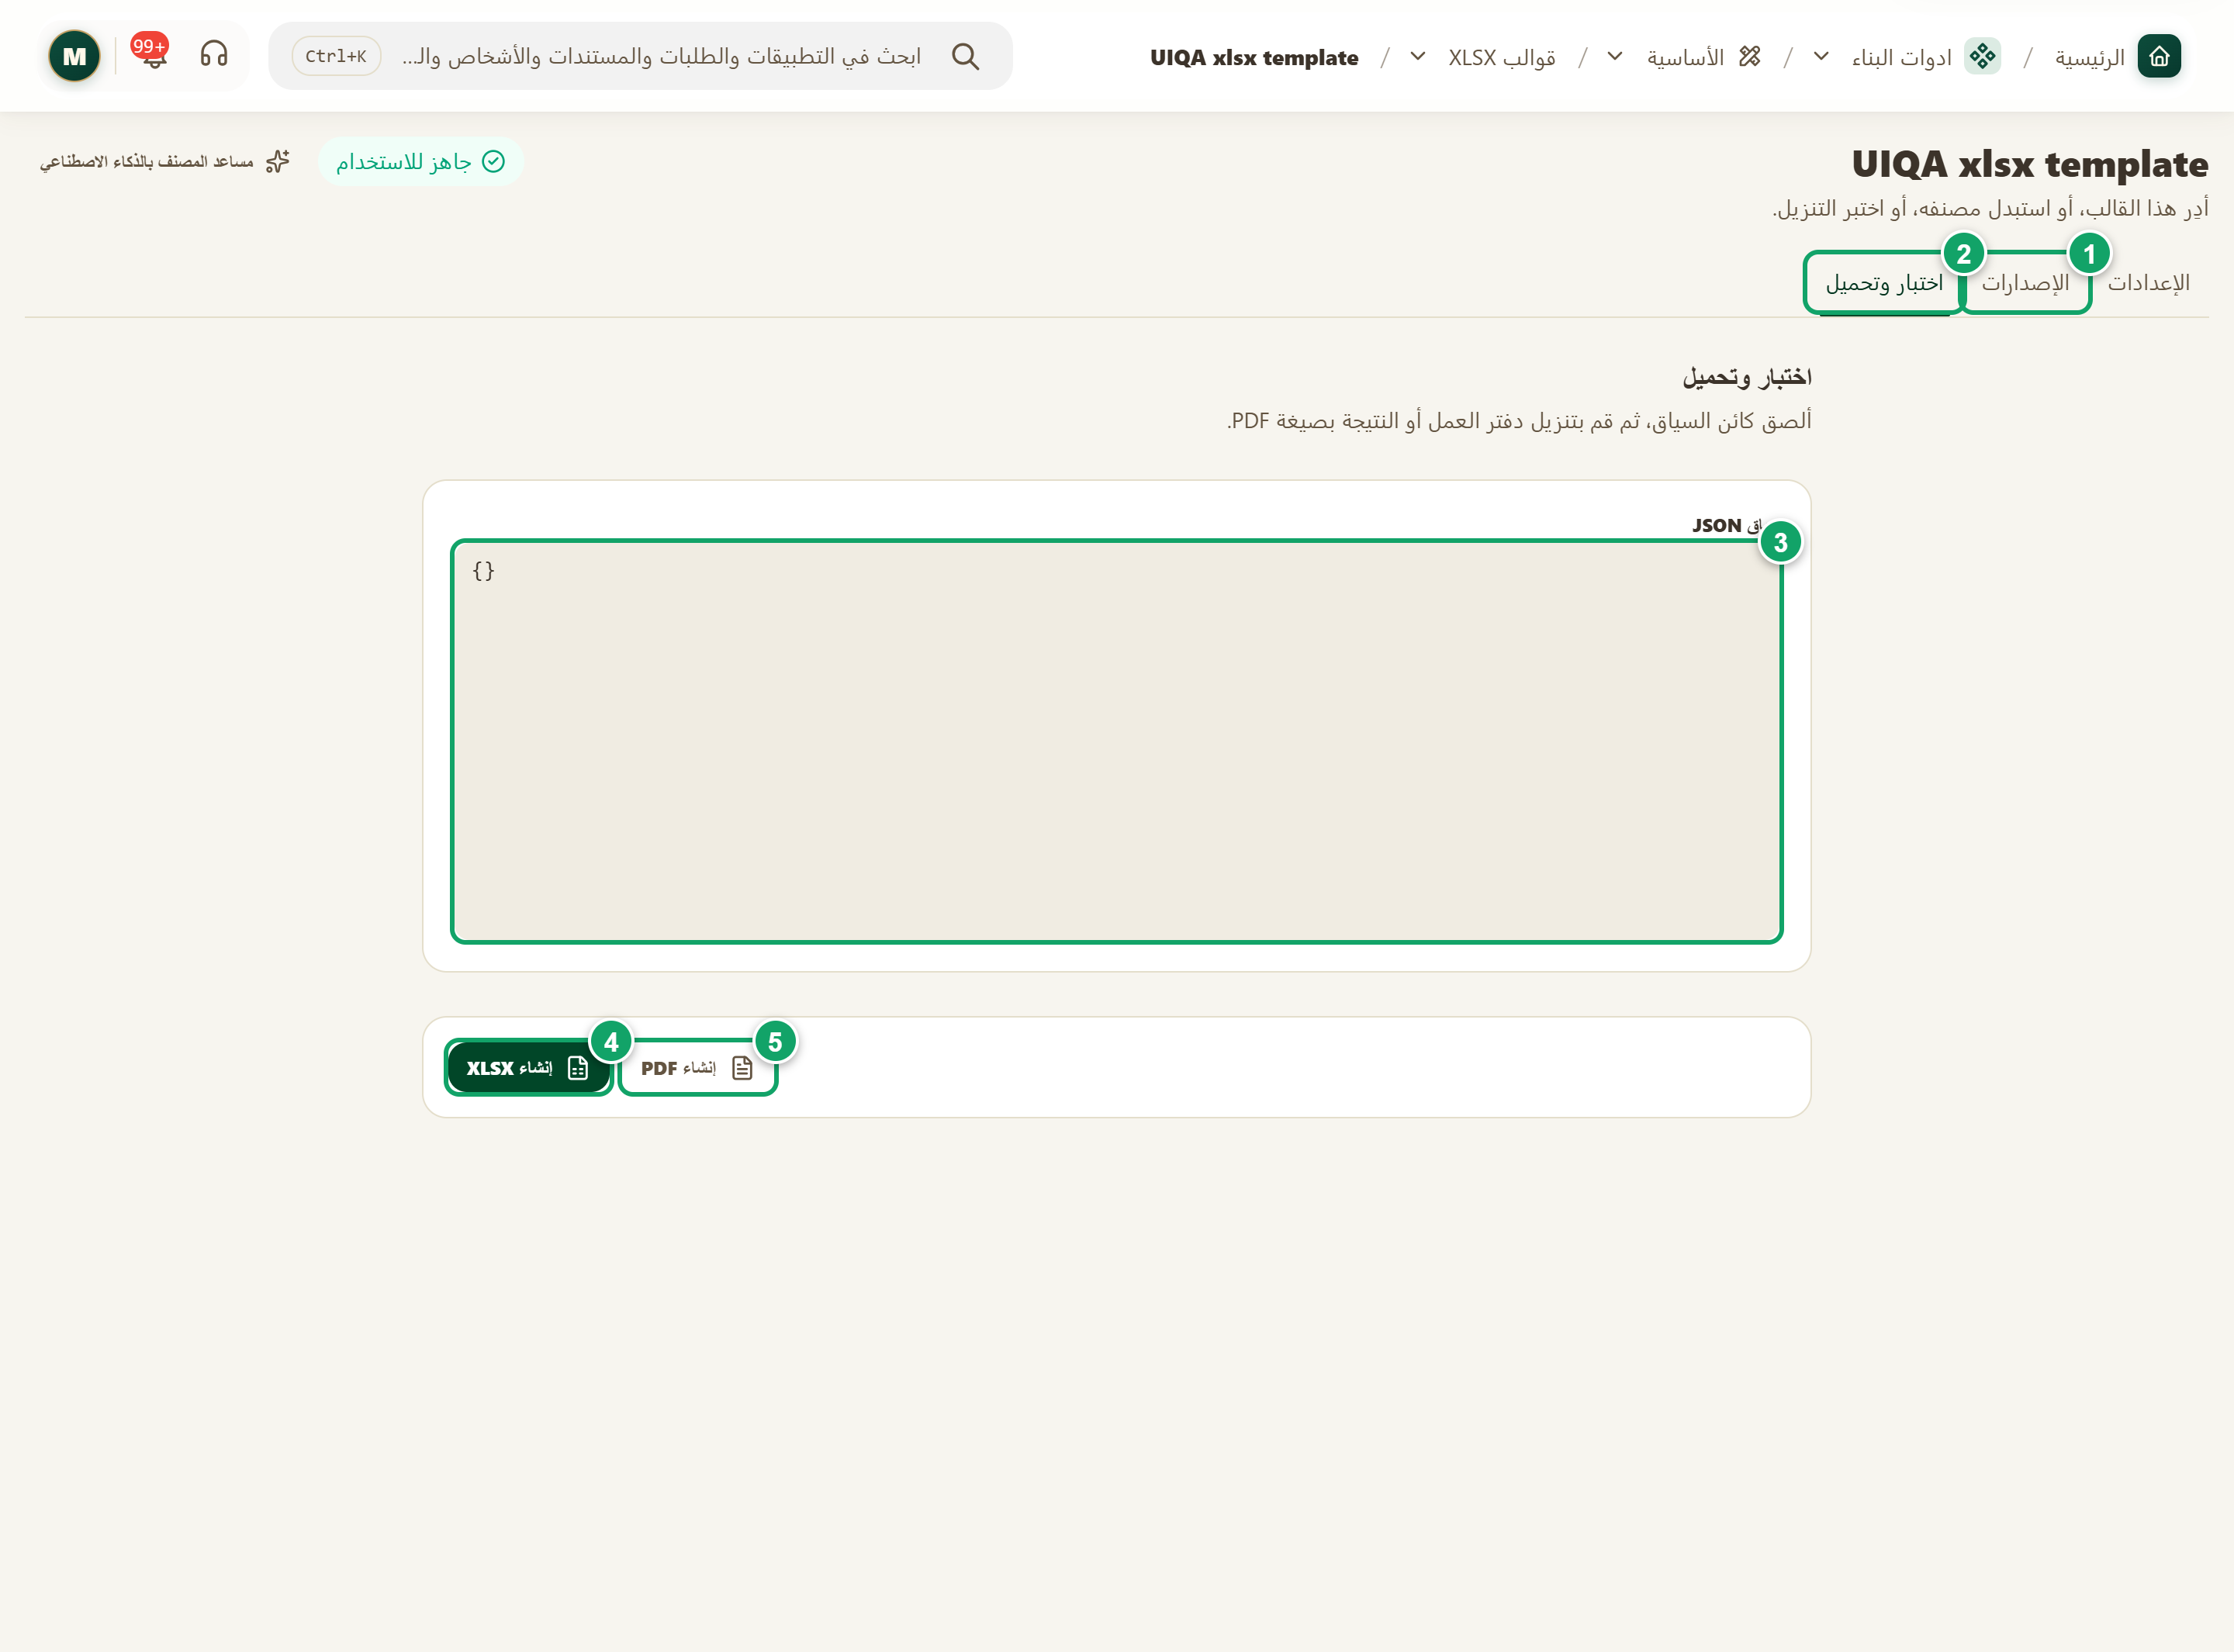
\includegraphics[width=0.95\linewidth,height=0.72\textheight,keepaspectratio]{figures/screens/ch06-xlsx-workspace-ar.png}
\caption{تبويب «اختبار وتحميل» في مساحة عمل قالب XLSX}
\label{fig:builder-xlsx-workspace-screen}
\shotnote{تعرض الصورة قالب XLSX اختبارياً في test2 مفتوحاً على «اختبار وتحميل»، ومربع السياق فيه فارغ إلا من القوسين. ويبيّن ذلك أن اختبار المصنف يعتمد على بيانات تكتبها بنفسك بصيغة JSON، لا على سجل تختاره كما في قوالب DOCX. ① «الإصدارات»: ترفع منه المصنف البديل. ② «اختبار وتحميل»: التبويب المعروض. ③ «سياق JSON»: تكتب فيه كائناً يحمل \en{\$record} وحقوله. ④ «إنشاء XLSX»: ينزّل ملف Excel لمراجعة الصفوف والصيغ. ⑤ «إنشاء PDF»: ينزّل ملف PDF لمراجعة الصفحات.}
\end{figure}

\begin{table}[H]
\centering
\caption{تبويبات مساحة العمل}
\label{tab:builder-xlsx-workspace-tabs}
\begin{tabularx}{\linewidth}{R{3.6cm} Y}
\rcHeaderRow
\thh{التبويب} & \thh{المحتوى والإجراء}\\
الإعدادات & «اسم القالب» و«الوصف» و«صيغة اسم الملف عند التنزيل» و«أذونات البيانات»، ثم «حفظ الإعدادات».\\
الإصدارات & في «استبدال المصنف» تختار ملفاً وتضغط زر التحقق والرفع، فلا يصبح حالياً إلا إذا نجح التحقق، وإلا ظهر «لم يُرفع هذا المصنف». ويعرض «سجل الإصدارات» الإصدارات من الأحدث مع علامة «الحالي».\\
اختبار وتحميل & تكتب بيانات الاختبار في «سياق JSON»، ثم تضغط «إنشاء XLSX» أو «إنشاء PDF» فيُنزَّل الملف.\\
مساعد المصنف & تكتب «تعليمات» تصف التغيير، وتؤكد إرسال سياق المصنف إلى مزود الذكاء الاصطناعي، ثم تضغط «إنشاء مسودة». وتراجعها بـ «تنزيل معاينة XLSX» و«مراجعة PDF»، ثم تضغط «اعتماد الإصدار» و«تأكيد الموافقة»، أو «حذف المسودة».\\
\end{tabularx}
\end{table}

\begin{table}[H]
\centering
\caption{ما الذي تراجعه في الملف الناتج؟}
\label{tab:builder-xlsx-workspace-checks}
\begin{tabularx}{\linewidth}{R{3.6cm} Y}
\rcHeaderRow
\thh{المراجعة} & \thh{النتيجة المتوقعة}\\
عدد الصفوف والأعمدة & يساوي عدد العناصر، مع الحفاظ على تنسيق الصف وعرض العمود.\\
الأنواع & تبقى الأرقام أرقاماً، والقيم المنطقية قيماً منطقية.\\
الصيغ والمخططات & تشير إلى النطاق الموسّع، وتظهر القيم الصحيحة بعد فتح الملف.\\
ملف PDF & منطقة الطباعة والهوامش والاتجاه وفواصل الصفحات والنص العربي سليمة.\\
\end{tabularx}
\end{table}

\begin{rcwarn}[المساعد لا يكتب فوق تعديل أحدث]
يحدد المساعد لكل تعديل الورقة والخلية ومحتواها المتوقع. فإذا تغيّر المصنف بعد الاقتراح فشل الاعتماد بدلاً من أن يكتب فوق الخلية الأحدث. ولا يعمل الاعتماد أيضاً قبل حل أسئلة ربط البيانات التي يطرحها المساعد.
\end{rcwarn}

\begin{figure}[H]
\centering
\begin{tikzpicture}[node distance=0.5cm]
\node[stepBox] (a) {\RL{فتح القالب}};
\node[stepBox,below=of a] (b) {\RL{استبدال المصنف أو}\\\RL{مسودة من المساعد}};
\node[stepBox,below=of b] (c) {\RL{التحقق من المصنف}};
\node[stepBox,below=of c] (d) {\RL{الاختبار بسياق JSON}};
\node[stepBox,below=of d] (e) {\RL{مراجعة XLSX وPDF}};
\draw[flowsTo] (a) -- (b);
\draw[flowsTo] (b) -- (c);
\draw[flowsTo] (c) -- (d);
\draw[flowsTo] (d) -- (e);
\end{tikzpicture}
\rclegend
\caption{دورة تحديث قالب XLSX}
\label{fig:builder-xlsx-workspace-flow}
\shotnote{يبيّن المخطط أن كل إصدار جديد يمر بالتحقق قبل أن يصبح حالياً، سواء رفعته بنفسك أو اعتمدته من المساعد. ثم يأتي الاختبار بالصيغتين، لأن نجاح ملف Excel لا يعني أن خدمة التحويل إلى PDF أنتجت صفحات سليمة.}
\end{figure}

\subsection{خطوات العمل والتحقق}
\begin{enumerate}
\item افتح القالب، وعدّل ما تحتاج إليه في «الإعدادات»، ثم اضغط «حفظ الإعدادات».
\item لاستبدال المصنف، افتح «الإصدارات» واختر الملف الجديد في «استبدال المصنف»، ثم اضغط زر التحقق والرفع.
\item افتح «اختبار وتحميل»، واكتب في «سياق JSON» كائناً فيه \en{\$record} وحقوله، مثل \en{\{"\$record": \{"total": 12\}\}}.
\item اضغط «إنشاء XLSX» وراجع الصفوف والصيغ، ثم اضغط «إنشاء PDF» وراجع الصفحات.
\end{enumerate}

\textbf{تحقق ومعالجة المشكلة:} يجب أن تظهر رسالة «تم تحميل نسخة XLSX.» وأن يحمل الإصدار الجديد علامة «الحالي». فإذا ظهر «أدخل كائن JSON صالح.»، فتأكد من أن النص يبدأ بقوس معقوص وينتهي به. وإذا نجح ملف Excel وفشل PDF، فالمشكلة في خدمة التحويل لا في القالب، فاطلب من مسؤول النظام التحقق منها.

\clearpage
\section{قوالب الطباعة}
\label{sec:builder-feature-print-templates}

قالب الطباعة مستند تصممه داخل كيان بالسحب والإفلات، دون أن ترفع ملف Word. ويطبع طلبات نموذج أو سجلات نوع معين بصيغة PDF أو Word، على ترويسة المؤسسة وهويتها. وتعرض صفحة «قوالب الطباعة» كل القوالب الموجودة وحالتها، أما إنشاء قالب جديد فيتم من داخل منشئ النموذج أو نوع السجلات بالضغط على «طباعة».

\textbf{المسار ومن يستخدمه:} «ادوات البناء» ← «الأساسية» ← «قوالب الطباعة». يستخدمها من يبني النماذج وأنواع السجلات.

\begin{rcnote}[مثال: شركة الأفق]
يفتح مسؤول النظام نوع «طلبات الزيارة» ويضغط «طباعة»، ثم يختار «ابدأ من نوع السجل هذا» ليصمم ورقة زيارة فيها رمز QR للتحقق، وينشرها فتظهر في زر «طباعة» داخل كل طلب. ويصل إلى القالب من ③.
\end{rcnote}

\begin{figure}[H]
\centering
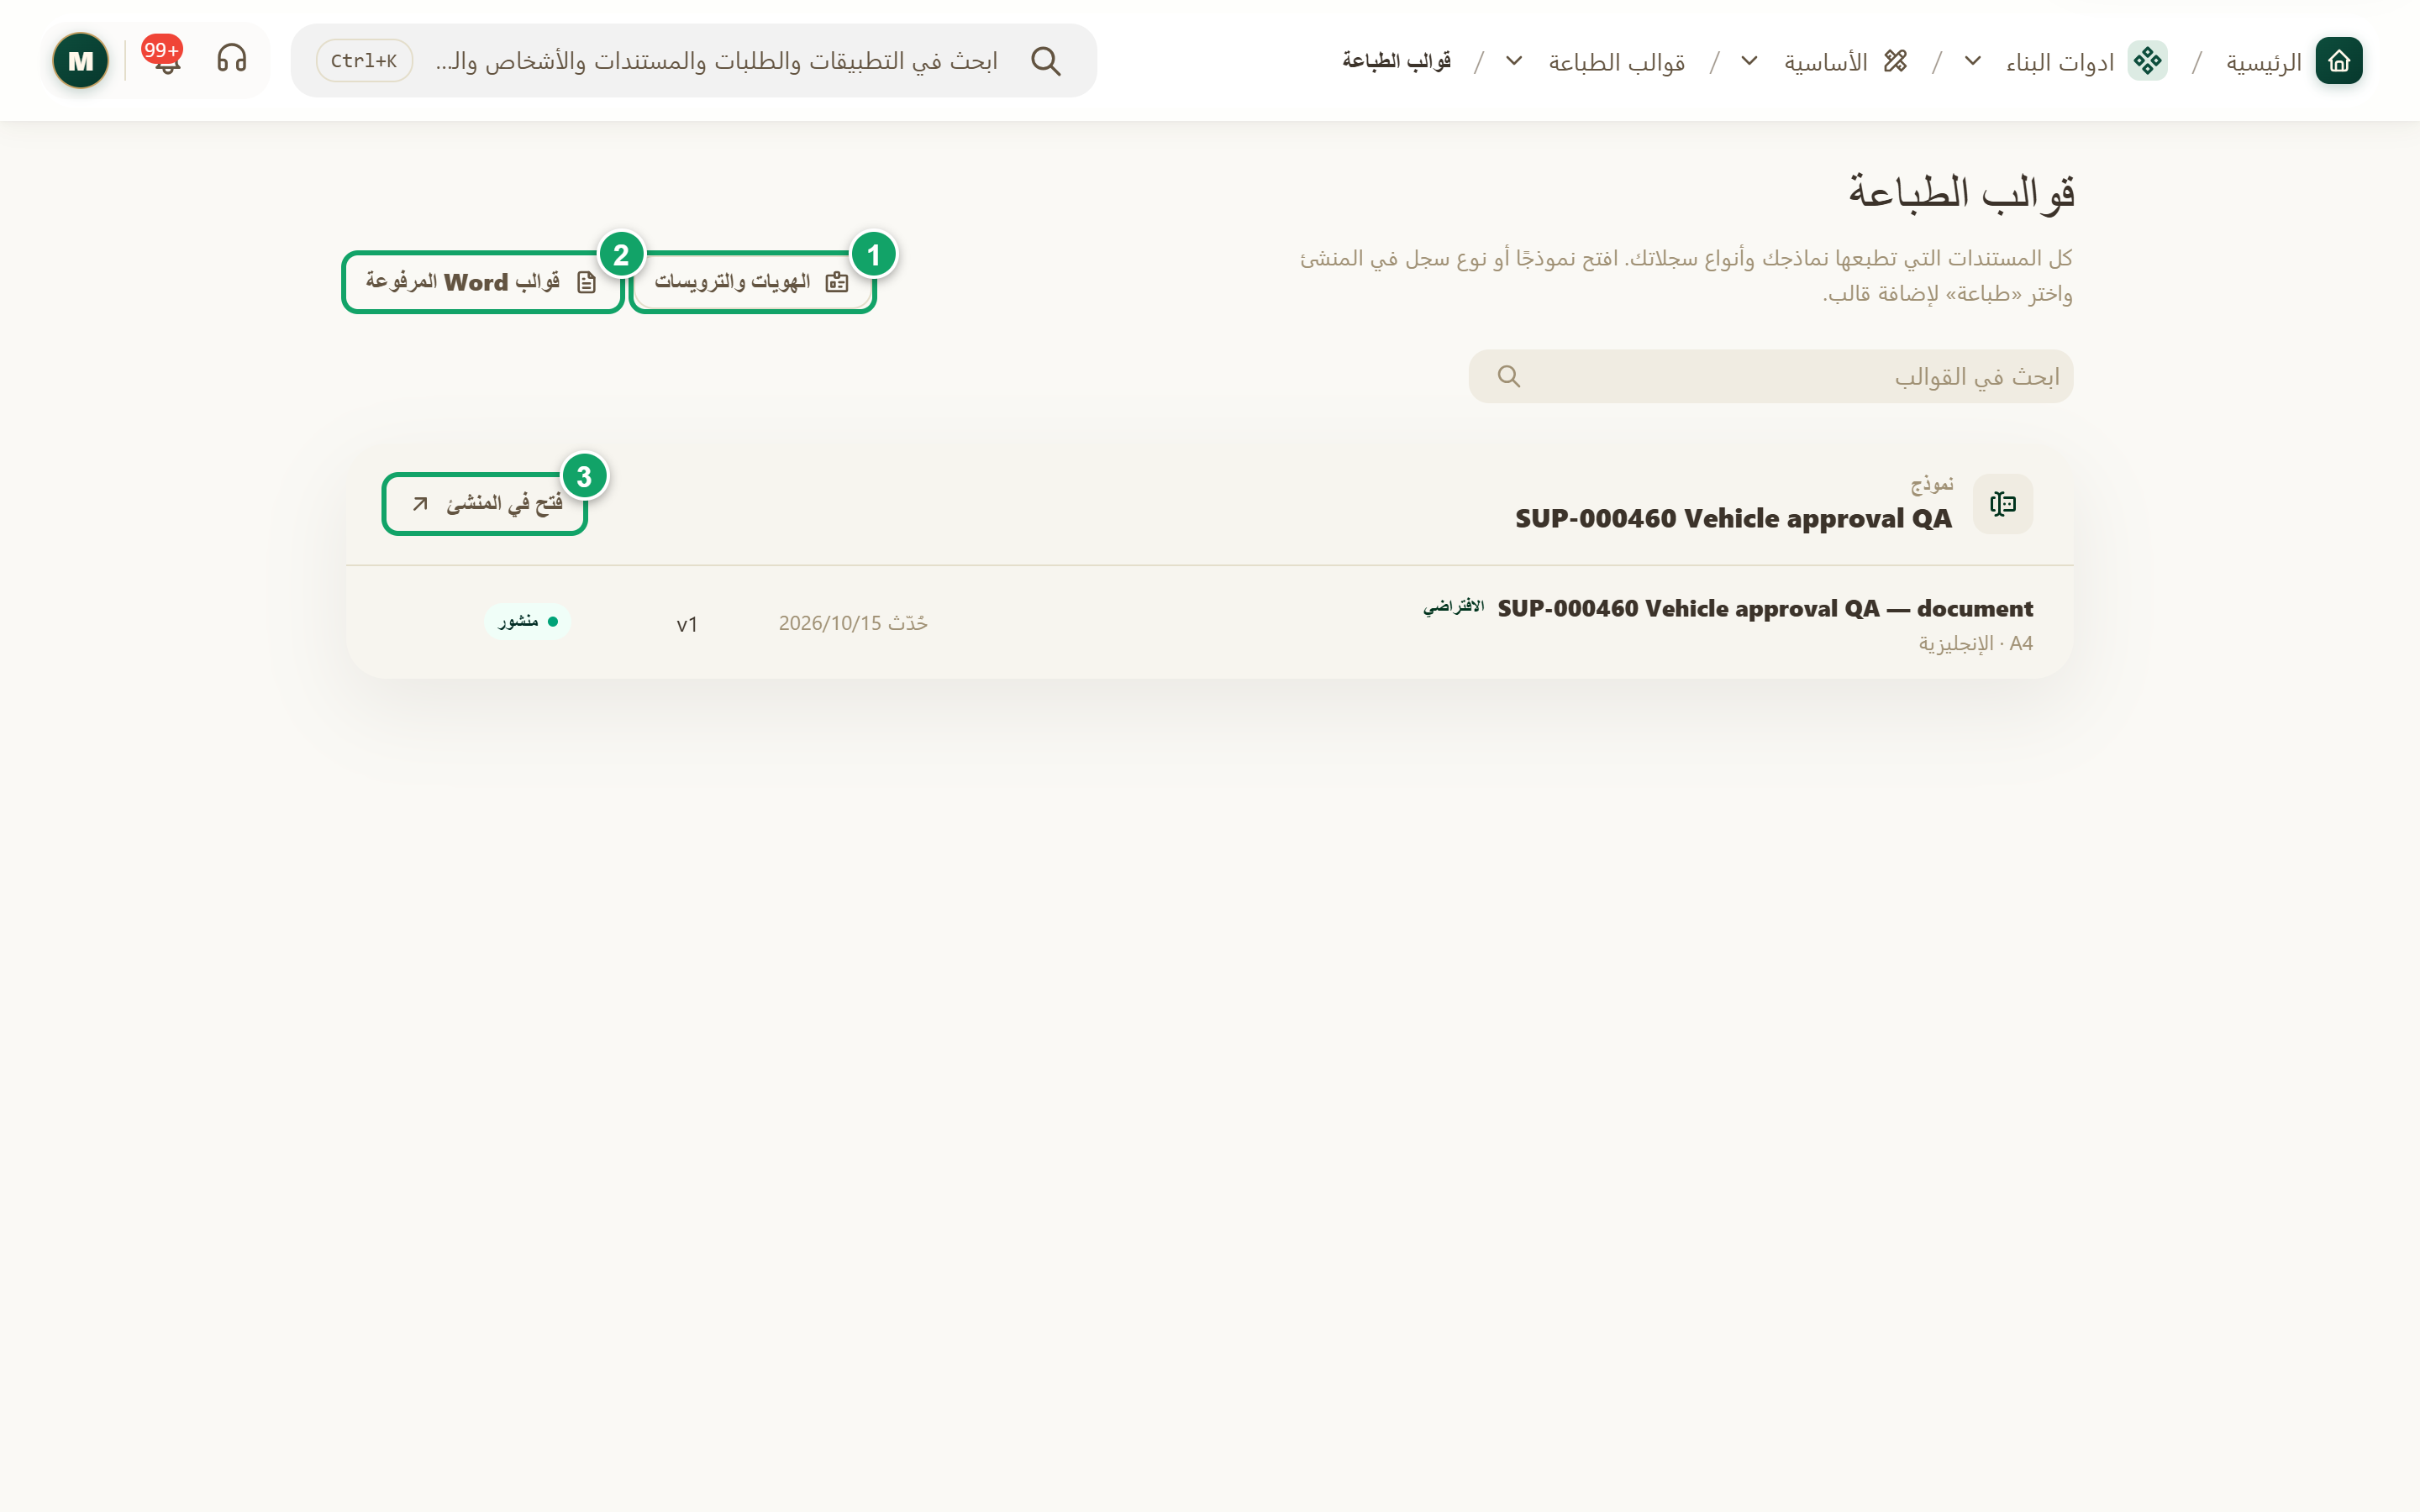
\includegraphics[width=0.95\linewidth,height=0.72\textheight,keepaspectratio]{figures/screens/ch06-print-ar.png}
\caption{مكتبة «قوالب الطباعة»}
\label{fig:builder-print-templates-screen}
\shotnote{تعرض الصفحة قوالب الطباعة مجمّعة حسب النموذج أو نوع السجلات، مع حالتها. والقالب الظاهر قالب اختبار. ① «الهويات والترويسات»: ينتقل إلى الشعارات والترويسات. ② «قوالب Word المرفوعة»: ينتقل إلى قوالب DOCX. ③ «فتح في المنشئ»: يفتح النموذج أو النوع حيث يُعدَّل القالب.}
\end{figure}


\begin{table}[H]
\centering
\caption{ما الذي تجده هنا؟}
\label{tab:builder-print-data}
\begin{tabularx}{\linewidth}{R{3.6cm} Y}
\rcHeaderRow
\thh{الجزء} & \thh{المحتوى والإجراء}\\
مكتبة القوالب & القوالب مجمّعة حسب النموذج أو نوع السجل، مع الحجم واللغة والإصدار والحالة: «منشور» أو «مسودة» أو «تغييرات غير منشورة»، وزر «فتح في المنشئ».\\
نافذة «قوالب الطباعة» & تفتح بزر «طباعة» في منشئ النموذج أو النوع، وتعرض لكل قالب «يُطبع من»: «قائمة الطباعة» أو «الطباعة الجماعية» أو «لا يظهر قبل النشر». ومنها «فتح» و«اجعله الافتراضي» و«أرشفة».\\
قالب جديد & من النافذة نفسها: «ابدأ من هذا النموذج» أو «ابدأ من نوع السجل هذا» أو «صفحة فارغة على ترويسة الجهة».\\
المخرجات & الصيغ المتاحة للتنزيل، واسم الملف، و«من يمكنه الطباعة»، والاحتفاظ بنسخة في السجل، وصفحة تحقق يفتحها رمز QR.\\
\end{tabularx}
\end{table}

\begin{figure}[H]
\centering
\begin{tikzpicture}[node distance=0.5cm]
\node[stepBox] (a) {\RL{طباعة من منشئ النموذج أو النوع}};
\node[stepBox,below=of a] (b) {\RL{تصميم البيانات والعناصر}};
\node[stepBox,below=of b] (c) {\RL{معاينة بسجل}};
\node[stepBox,below=of c] (d) {\RL{نشر}};
\node[stepBox,below=of d] (e) {\RL{زر طباعة في السجل}};
\draw[flowsTo] (a) -- (b);
\draw[flowsTo] (b) -- (c);
\draw[flowsTo] (c) -- (d);
\draw[flowsTo] (d) -- (e);
\end{tikzpicture}
\rclegend
\caption{من التصميم إلى زر الطباعة}
\label{fig:builder-print-flow}
\shotnote{يبيّن المخطط أن القالب يولد داخل منشئ النموذج أو نوع السجلات، لا في صفحة المكتبة، وأنه لا يظهر للمستخدمين قبل النشر. وتأتي المعاينة بسجل حقيقي قبل النشر لتكشف الحقول الفارغة أو الجداول الطويلة قبل أن يطبعها أحد.}
\end{figure}

\subsection{خطوات العمل والتحقق}
\begin{enumerate}
\item افتح النموذج أو نوع السجلات في المنشئ، واضغط «طباعة»، ثم اختر نقطة البداية.
\item أضف الحقول والعناصر، واضبط في «الصفحة» الورق والهوية والترويسة.
\item اضغط «معاينة بسجل» و«تنزيل ملف PDF تجريبي»، ثم حدد «من يمكنه الطباعة» واضغط «نشر».
\end{enumerate}

\textbf{تحقق ومعالجة المشكلة:} يجب أن يظهر القالب «منشور» في المكتبة، وأن يظهر في قائمة «اختر مستندًا» عند الضغط على «طباعة» في السجل. فإذا لم يظهر، فتأكد من نشره، لأن القالب «لا يظهر قبل النشر»؛ واستخدم «الفحص على جميع السجلات» لاكتشاف السجلات التي تنقصها بيانات.

\clearpage
\section{منشئ قالب الطباعة: البيانات والعناصر}
\label{sec:builder-feature-print-builder}

يفتح المنشئ عندما تختار نقطة بداية لقالب جديد أو تضغط «فتح» بجانب قالب موجود. وتظهر في وسطه الصفحة كما ستُطبع، وإلى جانبها ثلاثة تبويبات: «البيانات» و«العناصر» و«الصفحة»، وفي الجانب الآخر «الإعدادات» الخاصة بما تحدده على الصفحة. ويحفظ المنشئ عملك تلقائياً، فترى «جارٍ الحفظ…» ثم «تم الحفظ»، لكن التعديلات تبقى مسودة لا يراها أحد حتى تنشرها. وكل عنصر على الصفحة نص حقيقي في ملف PDF يمكن تحديده والبحث فيه، وليس صورة للصفحة.

\textbf{المسار ومن يستخدمه:} منشئ النموذج أو نوع السجلات ← «طباعة» ← نقطة بداية أو «فتح». يستخدمه من يبني النموذج أو نوع السجلات.

\begin{rcnote}[مثال: شركة الأفق]
يسحب مسؤول النظام حقل تاريخ الزيارة من مجموعة «هذا السجل» إلى ورقة الزيارة، ويختار له في «عندما يكون فارغًا» خيار «إيقاف الطباعة». ثم يضيف عنصر «إظهار عند» حول فقرة ملاحظات المراجعة، فلا تُطبع إلا إذا كتبت سارة الخطيب ملاحظة. ويأخذ الحقل من ①، وعنصر «إظهار عند» من ② ثم ③.
\end{rcnote}

\begin{figure}[H]
\centering
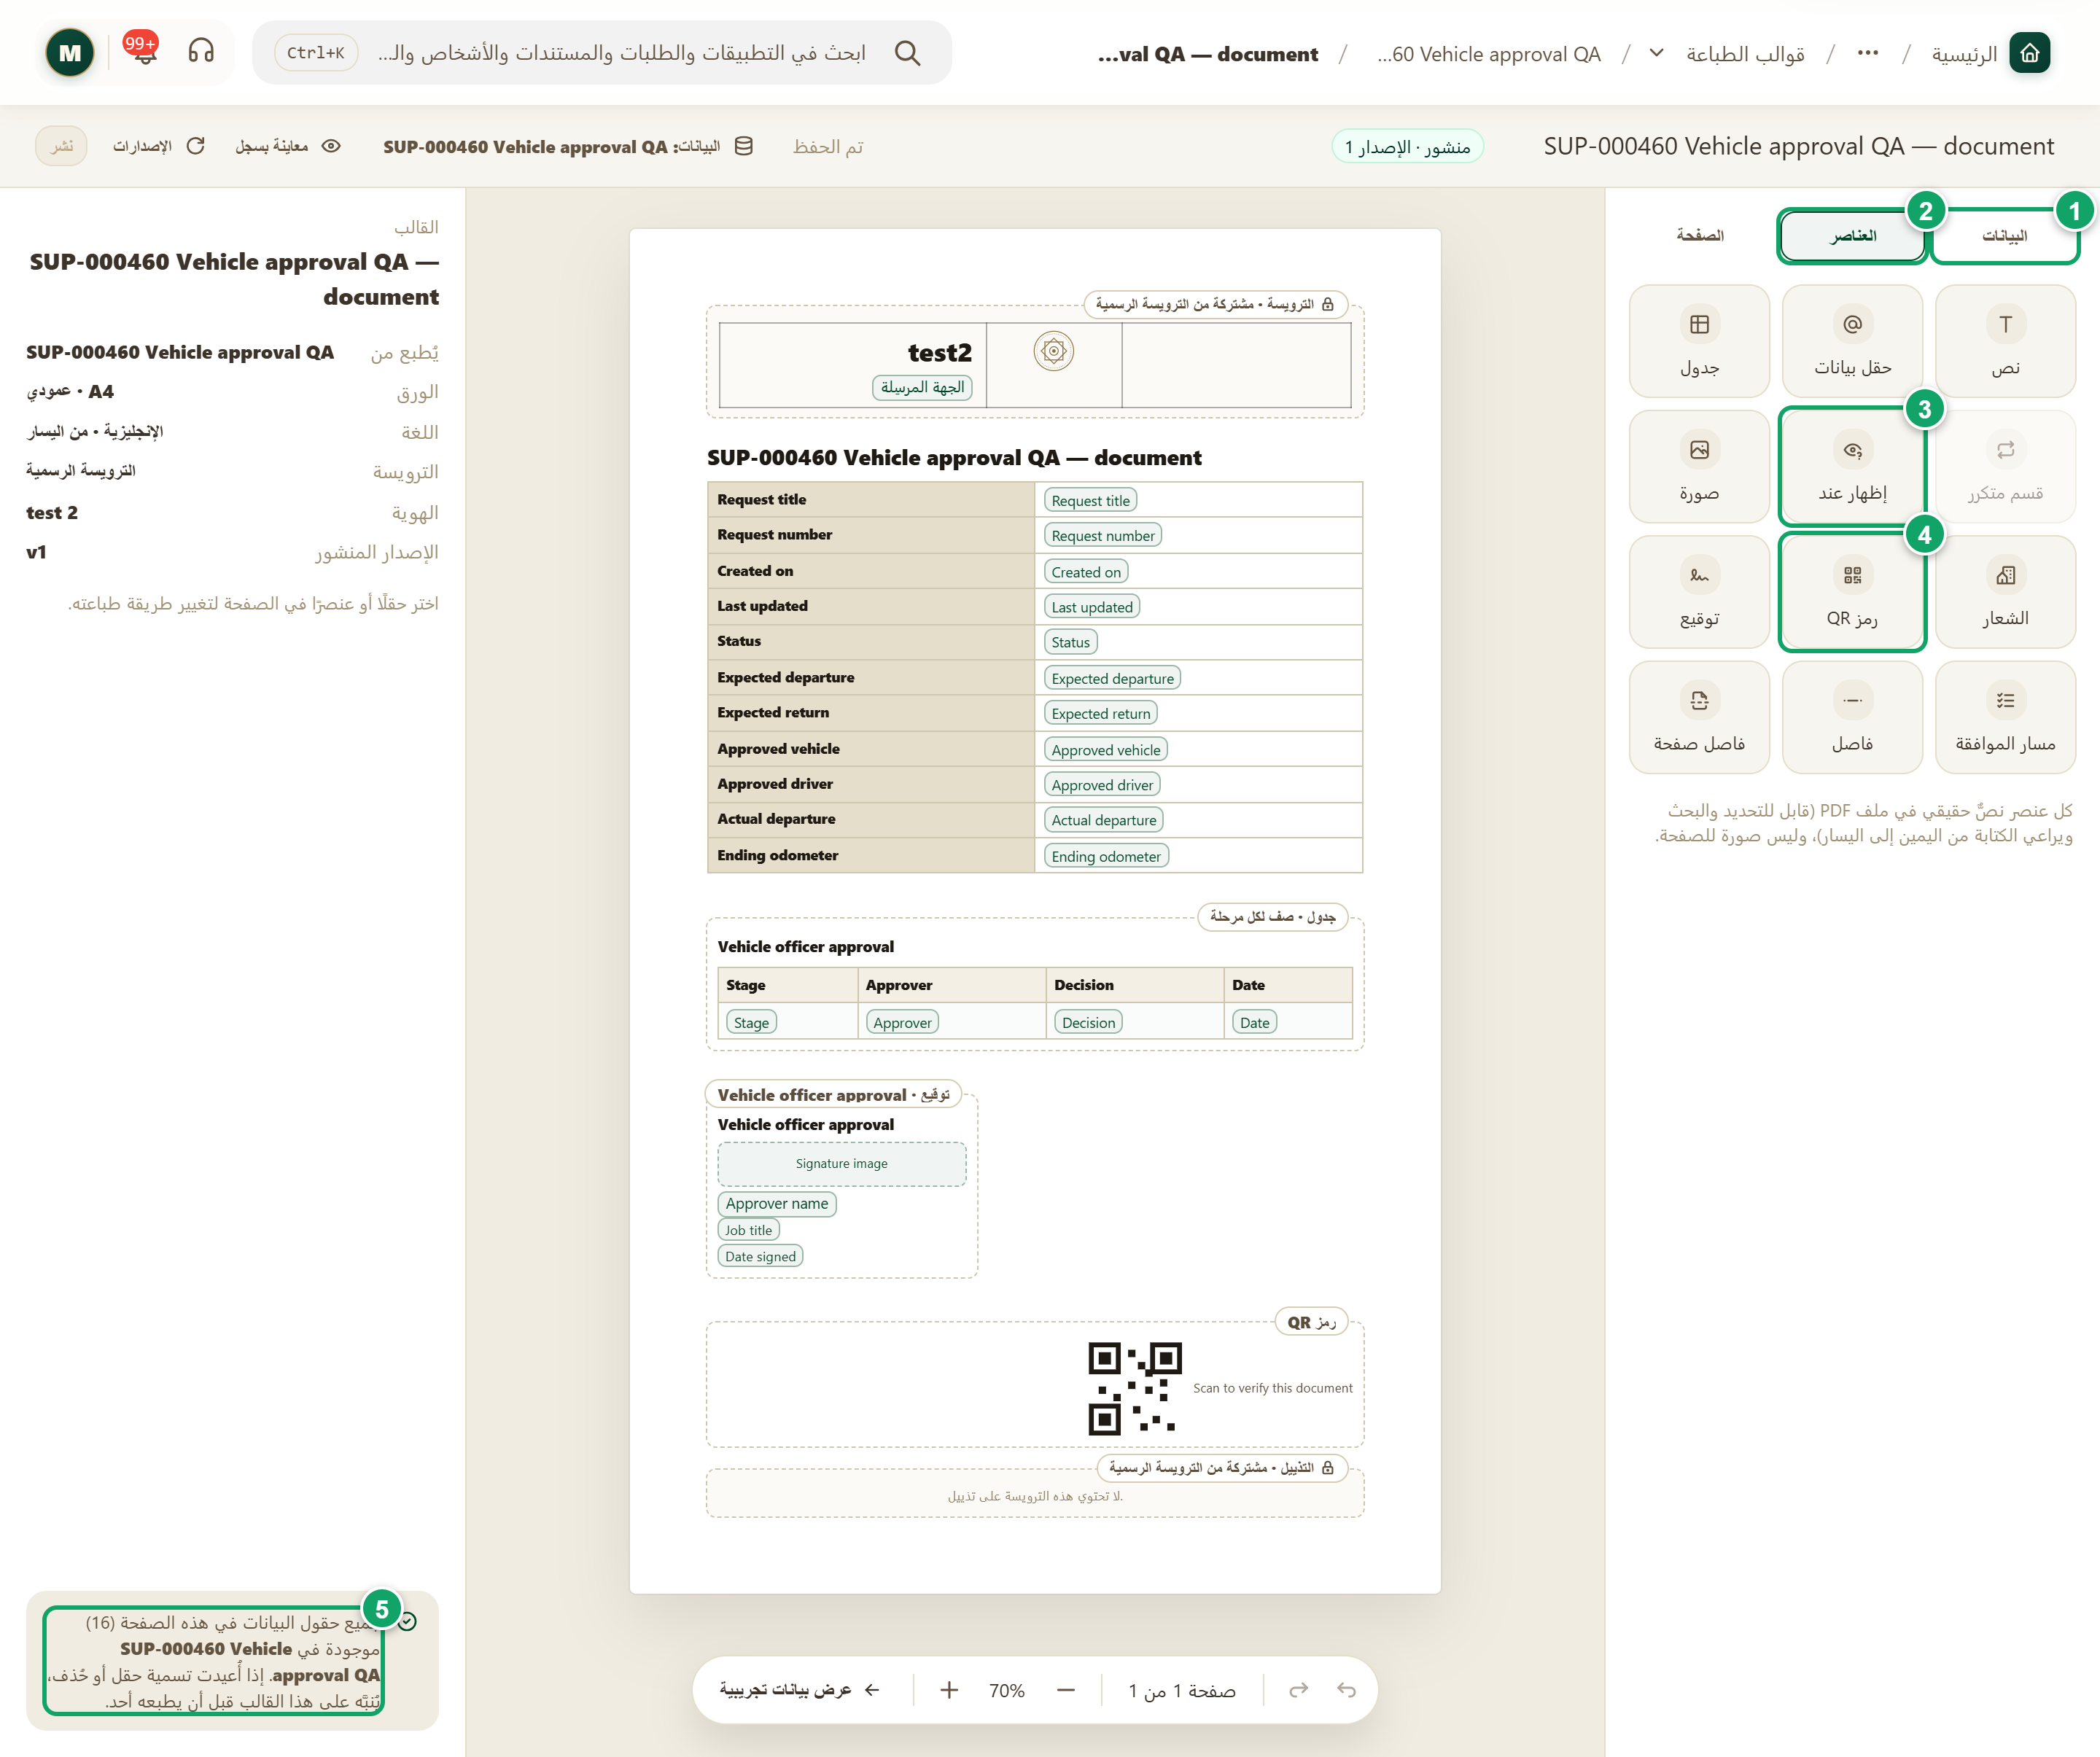
\includegraphics[width=0.95\linewidth,height=0.72\textheight,keepaspectratio]{figures/screens/ch06-print-builder-ar.png}
\caption{منشئ قالب الطباعة وتبويب «العناصر» مفتوح}
\label{fig:builder-print-builder-screen}
\shotnote{تعرض الصورة قالب طباعة اختبارياً لنموذج في test2 داخل المنشئ، والصفحة في الوسط كما ستُطبع بحقولها وجدول الموافقات والتوقيع ورمز QR. ويظهر «قسم متكرر» باهتاً لأن هذا النموذج لا يحتوي على قوائم، والعنصر لا يعمل إلا مع قائمة. ① «البيانات»: الحقول التي تسحبها إلى الصفحة. ② «العناصر»: التبويب المعروض. ③ «إظهار عند»: جزء لا يُطبع إلا إذا تحققت شروطه. ④ «رمز QR»: رمز يفتح صفحة التحقق. ⑤ شريط الحالة: يؤكد أن جميع حقول البيانات في الصفحة ما زالت موجودة.}
\end{figure}

\begin{table}[H]
\centering
\caption{تبويب «البيانات»}
\label{tab:builder-print-builder-data}
\begin{tabularx}{\linewidth}{R{3.6cm} Y}
\rcHeaderRow
\thh{المجموعة} & \thh{ما تحتويه}\\
«هذا الطلب» أو «هذا السجل» & حقول الطلب أو السجل الذي يُطبع، ولكل حقل نوعه، مثل نص أو تاريخ أو خيار.\\
«السجلات المرتبطة» & حقول السجلات التي يرتبط بها السجل، وتفتح حقولها بالضغط على اسمها.\\
«القوائم» & القوائم التي تصلح لعنصر «قسم متكرر»، مثل إجابات الجداول والسجلات المرتبطة.\\
«الموافقات والتوقيعات» & مراحل الموافقة ومن وقّع عليها، عندما يكون للنموذج أو النوع موافقات.\\
«الجهة» و«المستند» & البيانات الرسمية للهوية، وبيانات المستند مثل التاريخ ورقم الصفحة ورمز QR للتحقق.\\
\end{tabularx}
\end{table}

تضيف الحقل بسحبه إلى الصفحة، أو بكتابة \en{/} أثناء الكتابة ثم اختيار الحقل. ولا تظهر في القائمة إلا الحقول التي تستطيع قراءتها.

\begin{table}[H]
\centering
\caption{تبويب «العناصر»}
\label{tab:builder-print-builder-blocks}
\begin{tabularx}{\linewidth}{R{3.6cm} Y}
\rcHeaderRow
\thh{العنصر} & \thh{ما يضيفه}\\
«نص» و«حقل بيانات» & فقرة جديدة، أو حقل تختاره من تبويب «البيانات».\\
«جدول» & جدول ثابت لتنسيق الصفحة.\\
«قسم متكرر» & جدول فيه صف لكل عنصر من قائمة، وتحدد أعمدته وعنوانه وما يظهر عندما تكون القائمة فارغة.\\
«إظهار عند» & جزء لا يُطبع إلا عند تحقق كل شروطه، بأداة الشروط نفسها المستخدمة في قواعد النماذج.\\
«صورة» و«الشعار» & صورة من حقل صورة في الطلب، أو شعار الهوية التي يُطبع القالب باسمها.\\
«رمز QR» & رمز يفتح صفحة التحقق من المستند عند مسحه.\\
«توقيع» و«مسار الموافقة» & خانة توقيع لمرحلة موافقة تعرض الصورة والاسم والمسمى والتاريخ، أو جدولاً بمراحل الموافقة.\\
«فاصل» و«فاصل صفحة» & خط أفقي، أو بداية صفحة جديدة.\\
\end{tabularx}
\end{table}

\subsection{إعدادات حقل البيانات}

عندما تحدد حقلاً على الصفحة تظهر إعداداته. فللتاريخ تختار «التقويم»: «ميلادي» أو «هجري» أو «كلاهما»، ثم «التنسيق». وللرقم تختار مثلاً «بفواصل (1,250)» أو «مبلغ مالي». أما «عندما يكون فارغًا» فتحدد ما يحدث للحقل الفارغ: «عرض —» أو «إخفاء السطر» أو «إيقاف الطباعة»، والخيار الأخير يمنع الطباعة ويخبر الشخص بالحقل الذي يجب تعبئته.

\begin{figure}[H]
\centering
\begin{tikzpicture}[node distance=0.5cm]
\node[stepBox] (a) {\RL{اختيار نقطة البداية}};
\node[stepBox,below=of a] (b) {\RL{سحب الحقول من البيانات}};
\node[stepBox,below=of b] (c) {\RL{إضافة العناصر}};
\node[stepBox,below=of c] (d) {\RL{ضبط إعدادات كل حقل}};
\node[stepBox,below=of d] (e) {\RL{حفظ تلقائي في المسودة}};
\draw[flowsTo] (a) -- (b);
\draw[flowsTo] (b) -- (c);
\draw[flowsTo] (c) -- (d);
\draw[flowsTo] (d) -- (e);
\end{tikzpicture}
\rclegend
\caption{تصميم محتوى قالب الطباعة}
\label{fig:builder-print-builder-flow}
\shotnote{يرتب المخطط العمل من المحتوى إلى التفاصيل: الحقول أولاً، ثم العناصر التي تنظمها، ثم طريقة طباعة كل حقل. وينتهي بالمسودة لأن الحفظ التلقائي لا يعني النشر، فلا يرى المستخدمون أي تغيير حتى تنشر القالب.}
\end{figure}

\subsection{خطوات العمل والتحقق}
\begin{enumerate}
\item افتح النموذج أو نوع السجلات في المنشئ، واضغط «طباعة»، ثم اختر نقطة بداية أو اضغط «فتح» بجانب قالب.
\item افتح «البيانات»، واسحب الحقول إلى مواضعها، أو اكتب \en{/} أثناء الكتابة لإدراج حقل.
\item افتح «العناصر»، وأضف ما تحتاج إليه، مثل «قسم متكرر» لقائمة أو «رمز QR» للتحقق.
\item حدد كل حقل مهم، واضبط تنسيقه وما يحدث عندما يكون فارغاً.
\item راجع شريط الحالة أسفل الصفحة، وتأكد من أن كل حقول البيانات موجودة.
\end{enumerate}

\textbf{تحقق ومعالجة المشكلة:} يجب أن يظهر «تم الحفظ» في رأس المنشئ، وأن يذكر شريط الحالة أن جميع حقول البيانات في الصفحة موجودة. فإذا ظهر «أحد حقول البيانات لم يعد موجودًا»، فالحقل حُذف أو أُعيدت تسميته وسيُطبع بالرمز —، فاختر حقلاً آخر أو أزله. وإذا ظهر «تعذّر الحفظ»، فاضغط «إعادة المحاولة».

\clearpage
\section{إعدادات الصفحة في قالب الطباعة}
\label{sec:builder-feature-print-page}

يضبط تبويب «الصفحة» شكل الورقة التي يُطبع عليها القالب: حجمها واتجاهها ولغتها وهوامشها، والهوية التي تحمل شعارها، والترويسة التي تظهر في رأسها وتذييلها. ويمكنه أيضاً أن يطبع علامة مائية على المستند إلى أن يُعتمد الطلب. وتسري هذه الإعدادات على هذا القالب وحده، فقالب آخر قد يستخدم ورقاً أو ترويسة مختلفة.

\textbf{المسار ومن يستخدمه:} منشئ قالب الطباعة ← «الصفحة». يستخدمه من يصمم القالب.

\begin{rcnote}[مثال: شركة الأفق]
يختار مسؤول النظام لورقة الزيارة ورقاً A4 عمودياً باللغة العربية، وترويسة الأفق التي يظهر رأسها في الصفحة الأولى فقط. ويفعّل العلامة المائية «مسودة» حتى يصل الطلب إلى حالة معتمدة، فلا تخرج ورقة غير معتمدة دون هذه العلامة. ويضبط الورق في ② و③، ويختار الترويسة تحت ⑤.
\end{rcnote}

\begin{figure}[H]
\centering
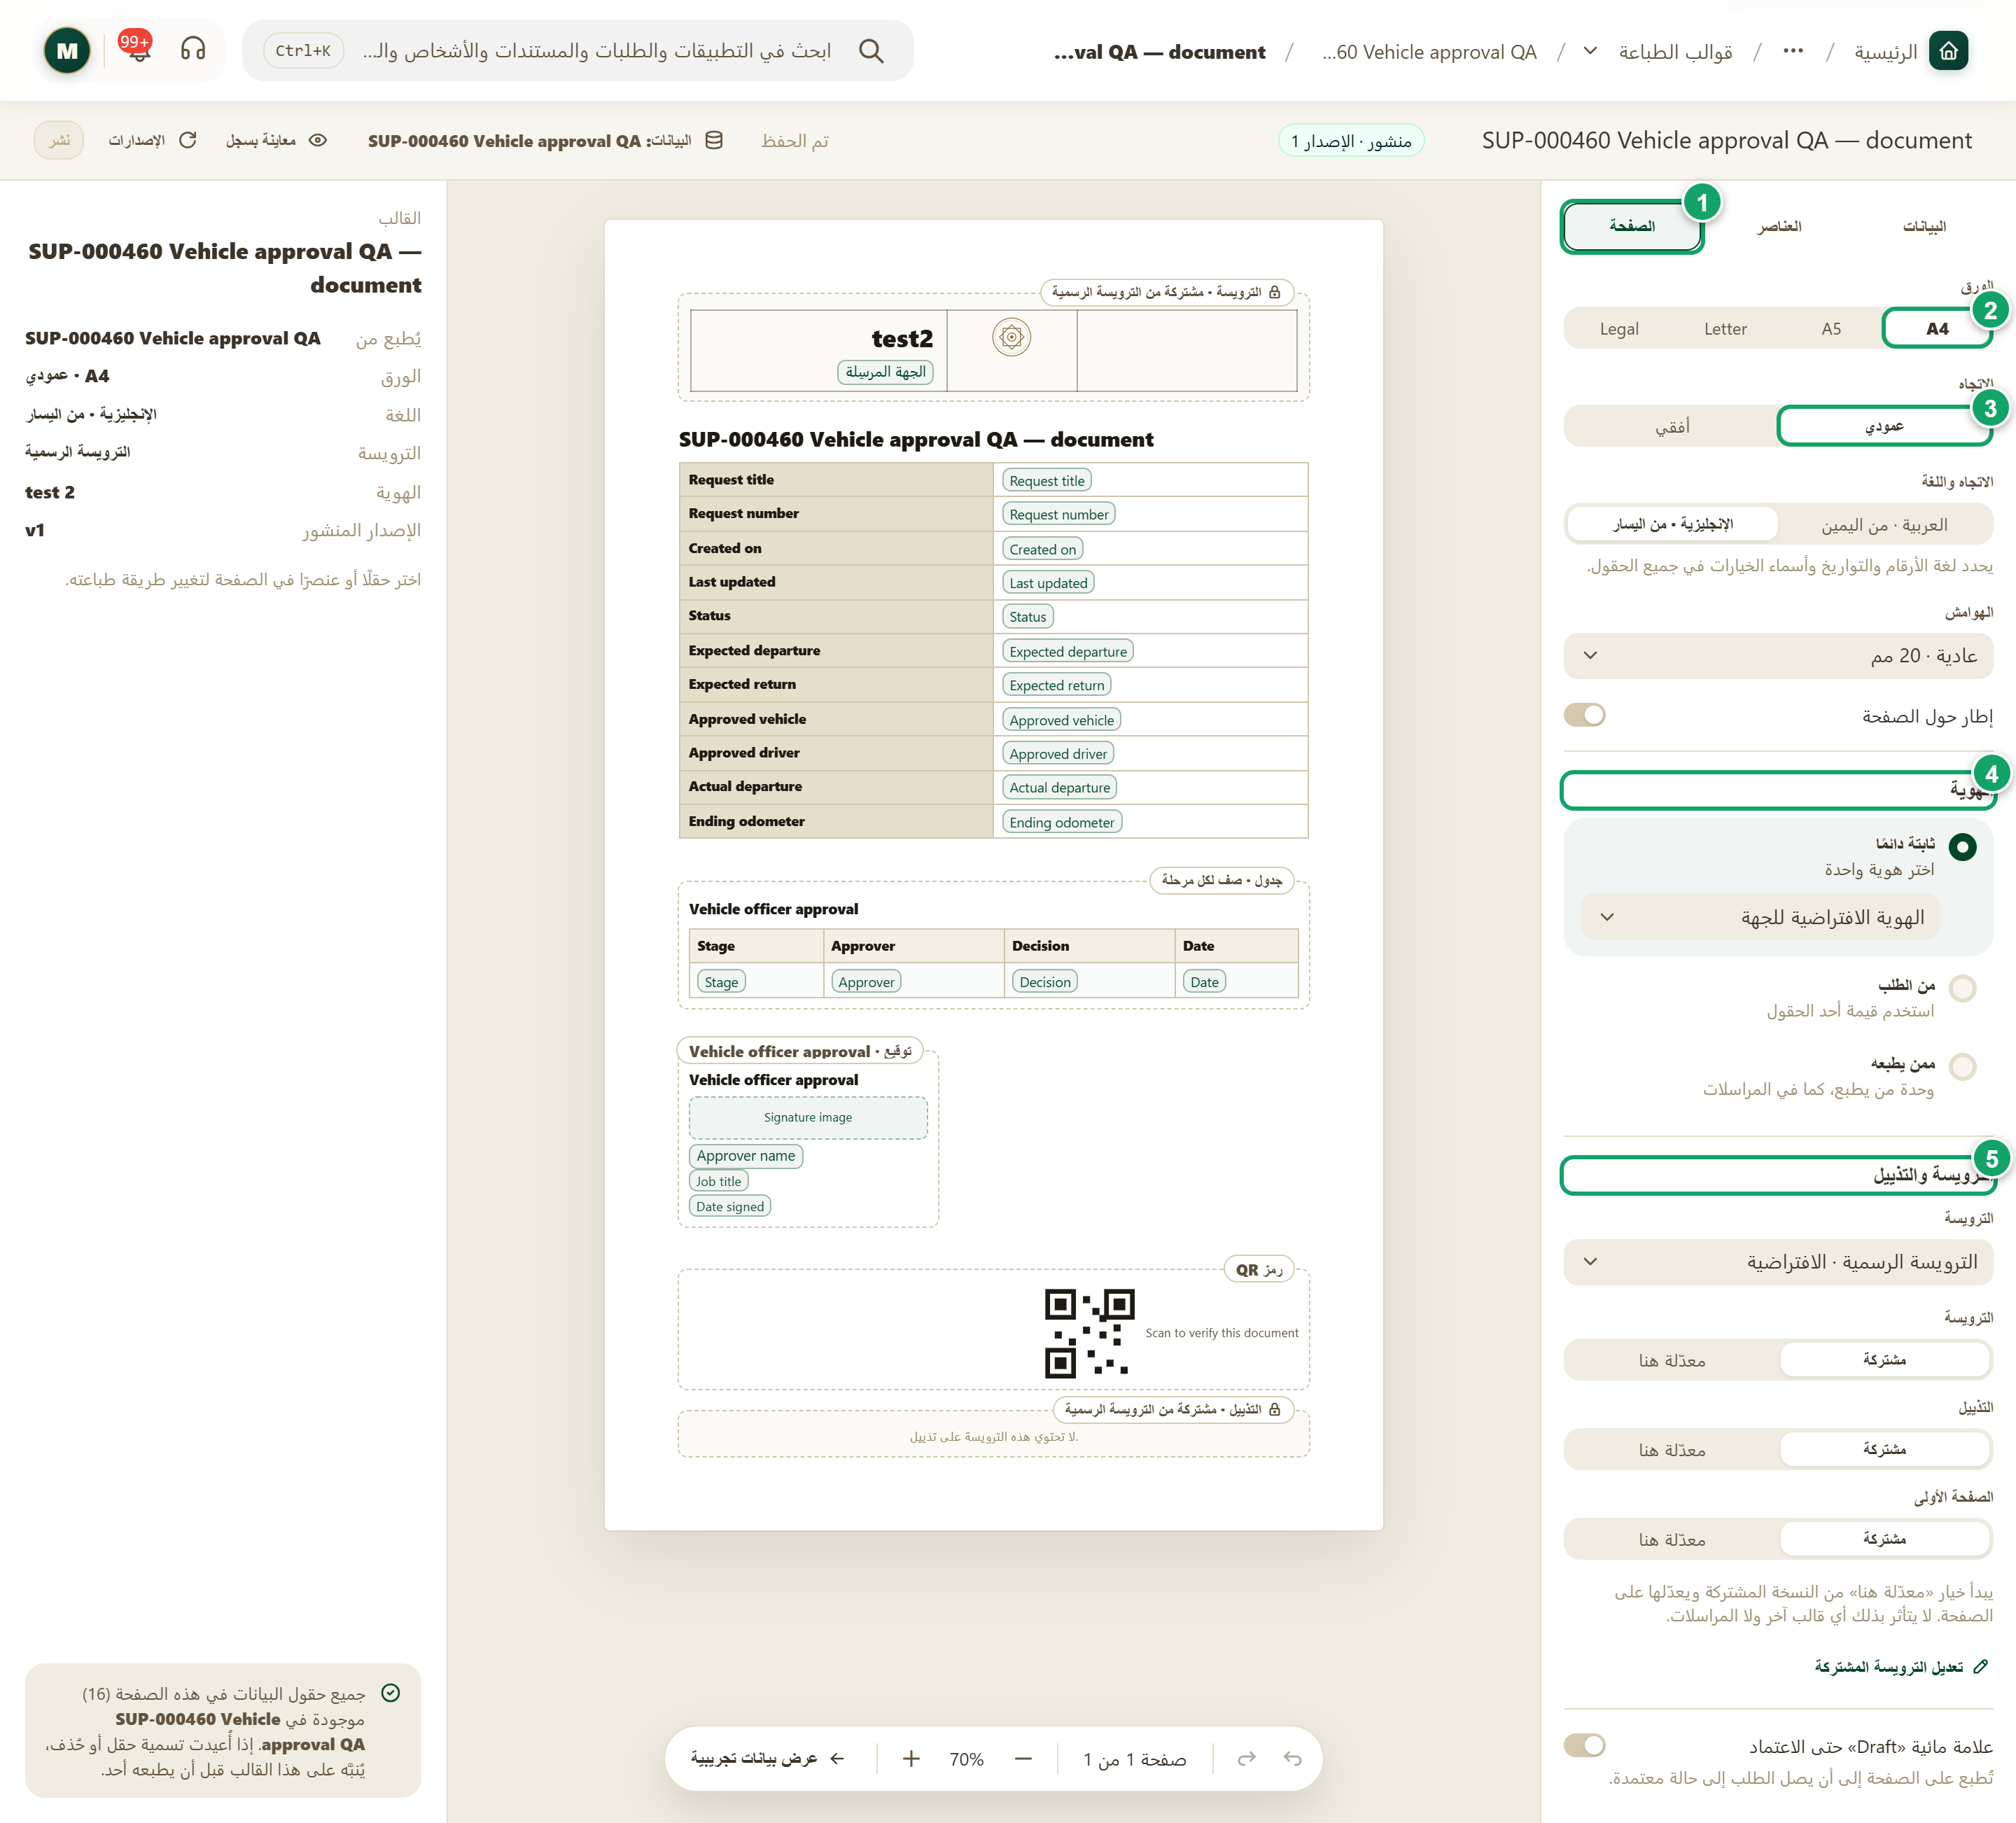
\includegraphics[width=0.95\linewidth,height=0.72\textheight,keepaspectratio]{figures/screens/ch06-print-page-ar.png}
\caption{تبويب «الصفحة» في منشئ قالب الطباعة}
\label{fig:builder-print-page-screen}
\shotnote{تعرض الصورة إعدادات الصفحة للقالب الاختباري نفسه: ورق A4 عمودي، والهوية الافتراضية للجهة، وترويسة مشتركة لم تُعدَّل في القالب. ويلخّص الجانب الآخر من المنشئ هذه الاختيارات، فتتأكد منها دون فتح كل إعداد. ① «الصفحة»: التبويب المعروض. ② «A4»: حجم الورق. ③ «عمودي»: اتجاه الورقة. ④ «الهوية»: مصدر الشعار والبيانات الرسمية. ⑤ «الترويسة والتذييل»: الترويسة المختارة، وهل تُستخدم كما هي أو تُعدَّل هنا.}
\end{figure}

\begin{table}[H]
\centering
\caption{إعدادات الورقة والهوية}
\label{tab:builder-print-page-paper}
\begin{tabularx}{\linewidth}{R{3.6cm} Y}
\rcHeaderRow
\thh{الإعداد} & \thh{الخيارات}\\
«الورق» و«الاتجاه» & A4 أو A5 أو Letter أو Legal، و«عمودي» أو «أفقي».\\
«الاتجاه واللغة» & «العربية · من اليمين» أو «الإنجليزية · من اليسار» أو «التركية · من اليسار»، وتحدد لغة الأرقام والتواريخ وأسماء الخيارات في كل الحقول.\\
«الهوامش» & «بلا هوامش» أو «ضيقة» أو «عادية» أو «عريضة» أو «مخصصة» بالمليمتر، مع خيار «إطار حول الصفحة».\\
«الهوية» & «ثابتة دائمًا» لهوية واحدة تختارها، أو «من الطلب» أو «من السجل» حسب قيمة أحد الحقول مع هوية بديلة للقيم الأخرى، أو «ممن يطبعه» حسب وحدة من يطبع.\\
العلامة المائية & «علامة مائية «مسودة» حتى الاعتماد»، وتختار في «لا علامة مائية عندما تكون الحالة» الحالات التي تختفي عندها. وإذا لم يكن للسجل حقل حالة، فتُطبع العلامة دائماً.\\
\end{tabularx}
\end{table}

\begin{table}[H]
\centering
\caption{«الترويسة والتذييل»}
\label{tab:builder-print-page-letterhead}
\begin{tabularx}{\linewidth}{R{3.6cm} Y}
\rcHeaderRow
\thh{الإعداد} & \thh{ما يفعله}\\
الترويسة & تختار ترويسة من الترويسات المشتركة، أو «بلا ترويسة».\\
«مشتركة» أو «معدّلة هنا» & تأخذ رأس الصفحة أو تذييلها من الترويسة المشتركة كما هي، أو تبدأ منها وتعدّلها على هذه الصفحة دون أن يتأثر أي قالب آخر أو المراسلات. ويعيدك «العودة إلى المشتركة» إلى الأصل.\\
الصفحات & في «تُطبع الترويسة في» و«يُطبع التذييل في» تختار «كل الصفحات» أو «الصفحة الأولى فقط».\\
تعديل الترويسة المشتركة & ينقلك إلى محرر الترويسة، وأي تعديل فيه يظهر في كل قالب يستخدمها.\\
«تغيّرت الترويسة المشتركة» & تنبيه يظهر بعد تعديل الترويسة المشتركة، ومنه «مقارنة» أو «اعتماد الجديدة» أو «الإبقاء على نسختي» للأجزاء التي عدّلتها هنا.\\
\end{tabularx}
\end{table}

\begin{figure}[H]
\centering
\begin{tikzpicture}[node distance=0.5cm]
\node[stepBox] (a) {\RL{الورق والاتجاه}};
\node[stepBox,below=of a] (b) {\RL{اللغة والهوامش}};
\node[stepBox,below=of b] (c) {\RL{الهوية}};
\node[stepBox,below=of c] (d) {\RL{الترويسة والتذييل}};
\node[stepBox,below=of d] (e) {\RL{العلامة المائية}};
\draw[flowsTo] (a) -- (b);
\draw[flowsTo] (b) -- (c);
\draw[flowsTo] (c) -- (d);
\draw[flowsTo] (d) -- (e);
\end{tikzpicture}
\rclegend
\caption{ضبط الصفحة من الورق إلى العلامة المائية}
\label{fig:builder-print-page-flow}
\shotnote{يتبع المخطط ترتيب الإعدادات في تبويب «الصفحة». وتسبق الهوية الترويسة لأن الترويسة تعرض شعار الهوية واسمها، فإذا تغيّرت الهوية تغيّر ما يظهر في رأس الصفحة.}
\end{figure}

\subsection{خطوات العمل والتحقق}
\begin{enumerate}
\item افتح تبويب «الصفحة»، واختر «الورق» و«الاتجاه»، ثم اللغة في «الاتجاه واللغة».
\item اختر الهامش المناسب، وفعّل «إطار حول الصفحة» إن احتجت إليه.
\item اختر في «الهوية» هوية ثابتة، أو اربطها بحقل في السجل إذا كان لكل فرع هوية.
\item اختر الترويسة، وحدد الصفحات التي يظهر فيها رأسها وتذييلها.
\item فعّل العلامة المائية إن أردت، واختر الحالات المعتمدة التي تختفي عندها.
\end{enumerate}

\textbf{تحقق ومعالجة المشكلة:} يجب أن تظهر الصفحة في المنشئ بالحجم والاتجاه والترويسة التي اخترتها، وأن يلخّص المنشئ الورق واللغة والترويسة والهوية. فإذا ظهر «تعذّر تحميل الترويسات وهويات الجهة»، فلا يمكن عرض القالب كما سيُطبع، فأعد المحاولة. وإذا أُرشفت الترويسة أو الهوية التي يستخدمها القالب، فاختر غيرها قبل الطباعة.

\clearpage
\section{المعاينة والنشر والطباعة من السجل}
\label{sec:builder-feature-print-publish}

قبل أن يصل القالب إلى المستخدمين تعاينه على سجل حقيقي، وتضبط مخرجاته، ثم تنشره. فزر «معاينة بسجل» في رأس المنشئ يفتح صفحة المعاينة، وفيها المستند كما سيُطبع وإعدادات «المخرجات» وزر النشر. وكل نشر ينشئ إصداراً جديداً، ويُسجَّل في كل ملف PDF الإصدار الذي أُنشئ به، فيمكن دائماً إعادة إنتاج أي نسخة مطبوعة قديمة. وبعد النشر يطبع المستخدمون المستند من زر «طباعة» في السجل.

\textbf{المسار ومن يستخدمه:} منشئ قالب الطباعة ← «معاينة بسجل». يستخدمه من يصمم القالب، أما زر «طباعة» فيستخدمه كل من يملك صلاحية الطباعة في السجل.

\begin{rcnote}[مثال: شركة الأفق]
يعاين مسؤول النظام ورقة الزيارة على الطلب HZN-VR-0001، ثم يقرأ نتيجة «الفحص على جميع السجلات» فيجد طلبين بلا تاريخ زيارة. ويختار «كل من يمكنه فتح السجل» وينشر الإصدار 1، فيطبع عمر حداد الورقة من زر «طباعة» في طلبه. فيختار الطلب من القائمة التي يبدأ بها ①، ويقرأ نتيجة الفحص فوق ②، ثم ينشر من ⑤.
\end{rcnote}

\begin{figure}[H]
\centering
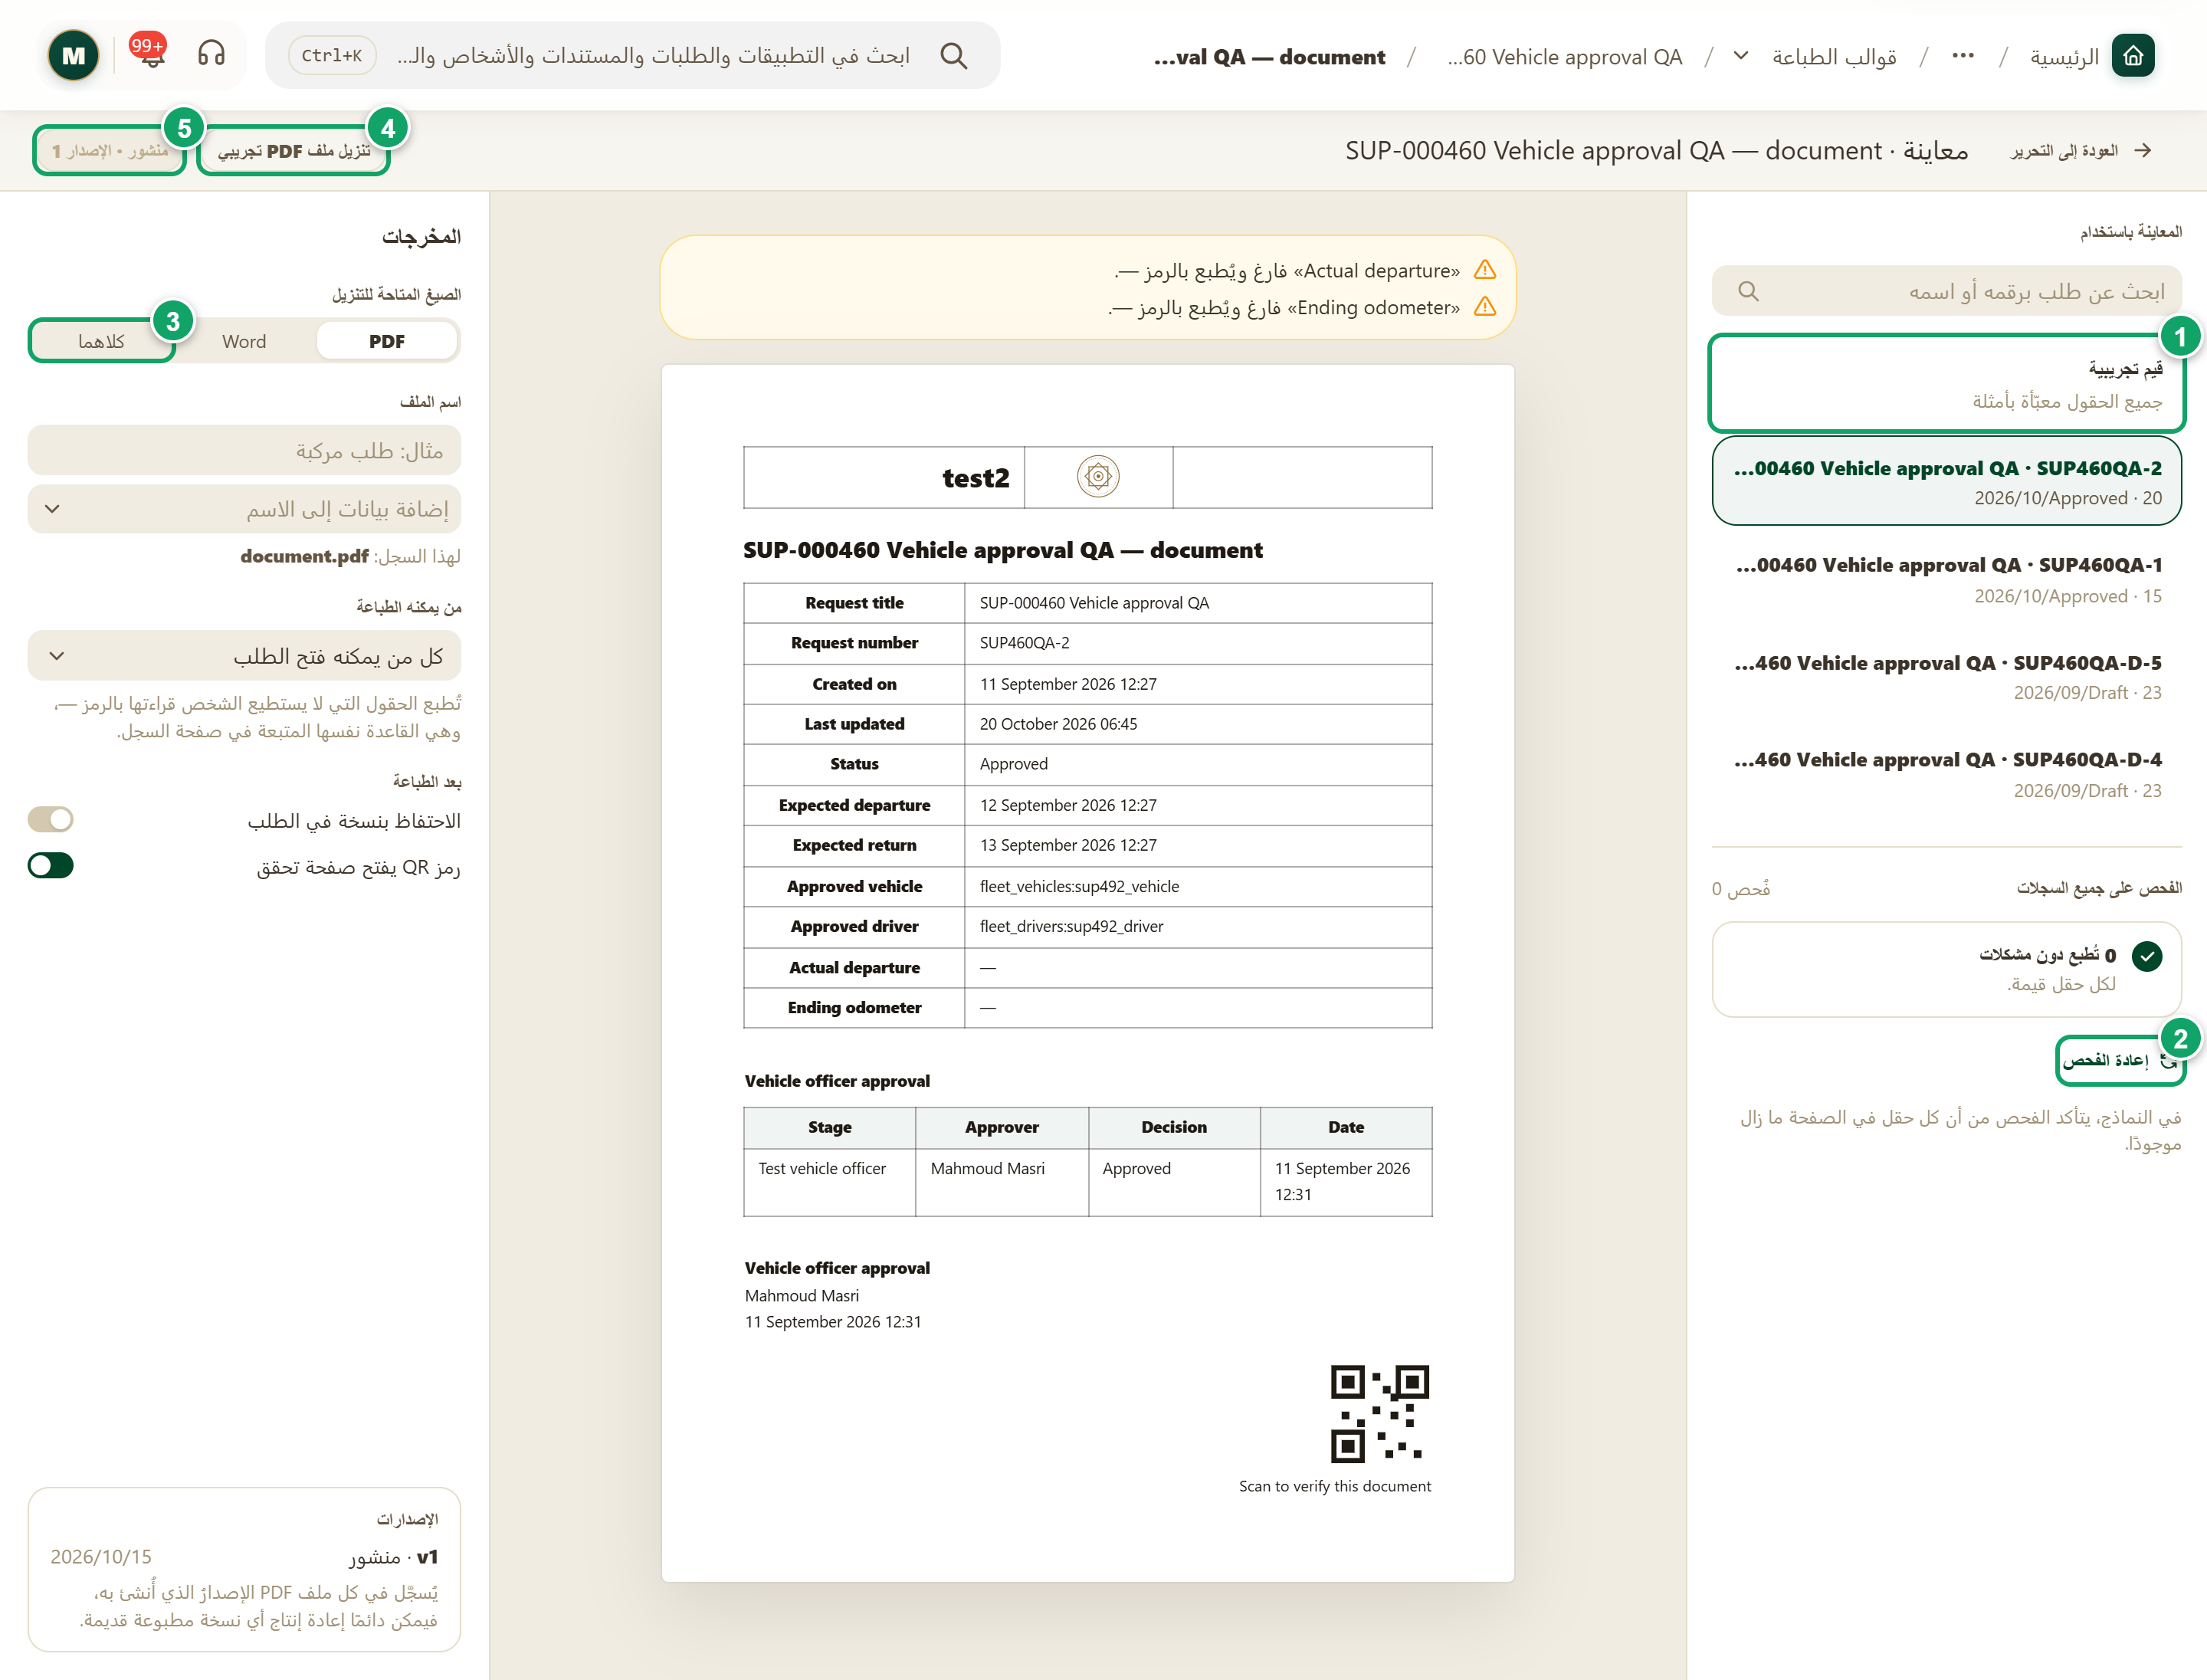
\includegraphics[width=0.95\linewidth,height=0.72\textheight,keepaspectratio]{figures/screens/ch06-print-publish-ar.png}
\caption{صفحة معاينة قالب الطباعة}
\label{fig:builder-print-publish-screen}
\shotnote{تعرض الصورة معاينة القالب الاختباري على طلب حقيقي في test2، ويظهر فوق المستند تنبيه بحقلين فارغين سيُطبعان بالرمز —. وتجمع الصفحة المعاينة والفحص والمخرجات، فتقرر النشر وأنت ترى النتيجة. ① «قيم تجريبية»: أول القائمة التي تختار منها أمثلة أو سجلاً حقيقياً. ② «إعادة الفحص»: يعيد «الفحص على جميع السجلات» بعد أي تعديل. ③ «كلاهما»: يسمح بتنزيل PDF وWord معاً. ④ «تنزيل ملف PDF تجريبي»: ينزّل المستند للسجل المختار. ⑤ زر النشر: يعرض «منشور · الإصدار 1» لأنه لا توجد تغييرات غير منشورة.}
\end{figure}

\begin{table}[H]
\centering
\caption{صفحة المعاينة}
\label{tab:builder-print-publish-preview}
\begin{tabularx}{\linewidth}{R{3.6cm} Y}
\rcHeaderRow
\thh{الجزء} & \thh{المحتوى والإجراء}\\
«المعاينة باستخدام» & تبحث عن سجل برقمه أو اسمه، أو تختار «قيم تجريبية» تملأ كل الحقول بأمثلة.\\
«الفحص على جميع السجلات» & يعمل تلقائياً عند فتح الصفحة، ويعيد زر «إعادة الفحص» تشغيله بعد أي تعديل. يفحص أحدث السجلات التي يمكنك فتحها، ويخبرك بعدد ما يُطبع دون مشكلات وبما ينقصه حقل أو يخفيه عن بعض الأشخاص. وفي النماذج يتأكد فقط من أن كل حقل ما زال موجوداً.\\
«تنزيل ملف PDF تجريبي» & ينزّل المستند للسجل المختار، ولا يعمل قبل اختيار سجل.\\
«المخرجات» & «الصيغ المتاحة للتنزيل»: PDF أو Word أو «كلاهما»؛ و«اسم الملف» مع «إضافة بيانات إلى الاسم»؛ و«من يمكنه الطباعة»: كل من يفتح السجل أو من يعدّله فقط؛ و«الاحتفاظ بنسخة في السجل»؛ و«رمز QR يفتح صفحة تحقق».\\
«نشر الإصدار N» & ينشر القالب، فتستخدم الطباعات الجديدة هذا الإصدار. ويعرض زر «الإصدارات» في رأس المنشئ الإصدارات المنشورة وتواريخها.\\
\end{tabularx}
\end{table}

\begin{table}[H]
\centering
\caption{الطباعة من السجل}
\label{tab:builder-print-publish-record}
\begin{tabularx}{\linewidth}{R{3.6cm} Y}
\rcHeaderRow
\thh{الإجراء} & \thh{ما يحدث}\\
«طباعة» ← «اختر مستندًا» & يعرض القوالب المنشورة، والقالب الافتراضي أولاً.\\
«تنزيل PDF» أو «اطبع الآن» أو «تنزيل ملف Word» & ينشئ المستند بالصيغ التي سمحت بها في «المخرجات».\\
«النسخ المطبوعة» & يعرض النسخ المحفوظة إذا فعّلت الاحتفاظ بنسخة في السجل.\\
«املأ هذه الحقول قبل الطباعة» & يظهر عندما يكون حقل مضبوط على «إيقاف الطباعة» فارغاً.\\
الطباعة الجماعية & تحدد عدة سجلات في جدول نوع السجلات وتضغط «طباعة»، ثم تختار ملف PDF واحداً أو ملف Word واحداً أو ملفاً مضغوطاً. وتُتخطّى السجلات التي لا يمكنك فتحها وتُذكر لك.\\
\end{tabularx}
\end{table}

\begin{figure}[H]
\centering
\begin{tikzpicture}[node distance=0.5cm]
\node[stepBox] (a) {\RL{معاينة بسجل}};
\node[stepBox,below=of a] (b) {\RL{الفحص على جميع السجلات}};
\node[stepBox,below=of b] (c) {\RL{ضبط المخرجات}};
\node[stepBox,below=of c] (d) {\RL{نشر الإصدار}};
\node[stepBox,below=of d] (e) {\RL{طباعة من السجل}};
\draw[flowsTo] (a) -- (b);
\draw[flowsTo] (b) -- (c);
\draw[flowsTo] (c) -- (d);
\draw[flowsTo] (d) -- (e);
\end{tikzpicture}
\rclegend
\caption{من المعاينة إلى أول نسخة مطبوعة}
\label{fig:builder-print-publish-flow}
\shotnote{يضع المخطط الفحص الشامل بعد معاينة سجل واحد، لأن سجلاً سليماً لا يضمن أن بقية السجلات تملك الحقول نفسها. ويأتي ضبط المخرجات قبل النشر، فهو الذي يحدد الصيغ ومن يطبع وما إذا كان المستند يحمل رمز تحقق.}
\end{figure}

\subsection{خطوات العمل والتحقق}
\begin{enumerate}
\item اضغط «معاينة بسجل»، وابحث عن سجل حقيقي في «المعاينة باستخدام».
\item راجع نتيجة «الفحص على جميع السجلات»، واضغط «إعادة الفحص» بعد أي تعديل، وعالج ما يظهر من حقول ناقصة أو محذوفة.
\item اضبط «المخرجات»: الصيغ، واسم الملف، و«من يمكنه الطباعة»، والاحتفاظ بنسخة، ورمز التحقق.
\item اضغط «تنزيل ملف PDF تجريبي» وراجع الملف، ثم اضغط «نشر الإصدار N».
\item افتح سجلاً، واضغط «طباعة»، واختر القالب ونزّل المستند.
\end{enumerate}

\textbf{تحقق ومعالجة المشكلة:} يجب أن تظهر رسالة «نُشر الإصدار N. ستستخدم الطباعات الجديدة هذا الإصدار.» وأن يظهر القالب في «اختر مستندًا». فإذا ظهر «تعذّر حفظ آخر تعديلاتك، لذلك لم يُنشر شيء»، فعالج مشكلة الحفظ ثم انشر مرة أخرى. وإذا طُبع حقل بالرمز —، فقد يكون فارغاً أو لا يملك الشخص صلاحية قراءته.

\clearpage
\section{صفحة التحقق من المستند}
\label{sec:builder-feature-print-verify}

عندما تفعّل «رمز QR يفتح صفحة تحقق» في مخرجات القالب، يحمل كل مستند مطبوع رمز تحقق خاصاً به. ويفتح مسح الرمز صفحة عامة لا تحتاج إلى تسجيل الدخول، تعرض المستند كما صدر وبياناته الأساسية. وبذلك يستطيع من يستلم الورقة، داخل المؤسسة أو خارجها، أن يتأكد من أنها صادرة فعلاً وأن محتواها لم يتغير. لكن الرمز يوثّق المستند الذي صدر، لا الورقة التي يظهر عليها، لذلك يقارن القارئ بين الاثنين.

\textbf{المسار ومن يستخدمه:} مسح رمز QR المطبوع على المستند، أو فتح رابطه. يستخدمها مستلم المستند، أما من يصمم القالب فيفعّلها من «المخرجات».

\begin{rcnote}[مثال: شركة الأفق]
يستلم فرع حلب ورقة الزيارة المطبوعة للطلب HZN-VR-0001، فيمسح موظف الاستقبال رمزها. فتظهر صفحة «الرمز موثّق» ومعها المستند كما صدر، فيقارن التاريخ والأسماء بالورقة التي بين يديه.
\end{rcnote}

\begin{figure}[H]
\centering
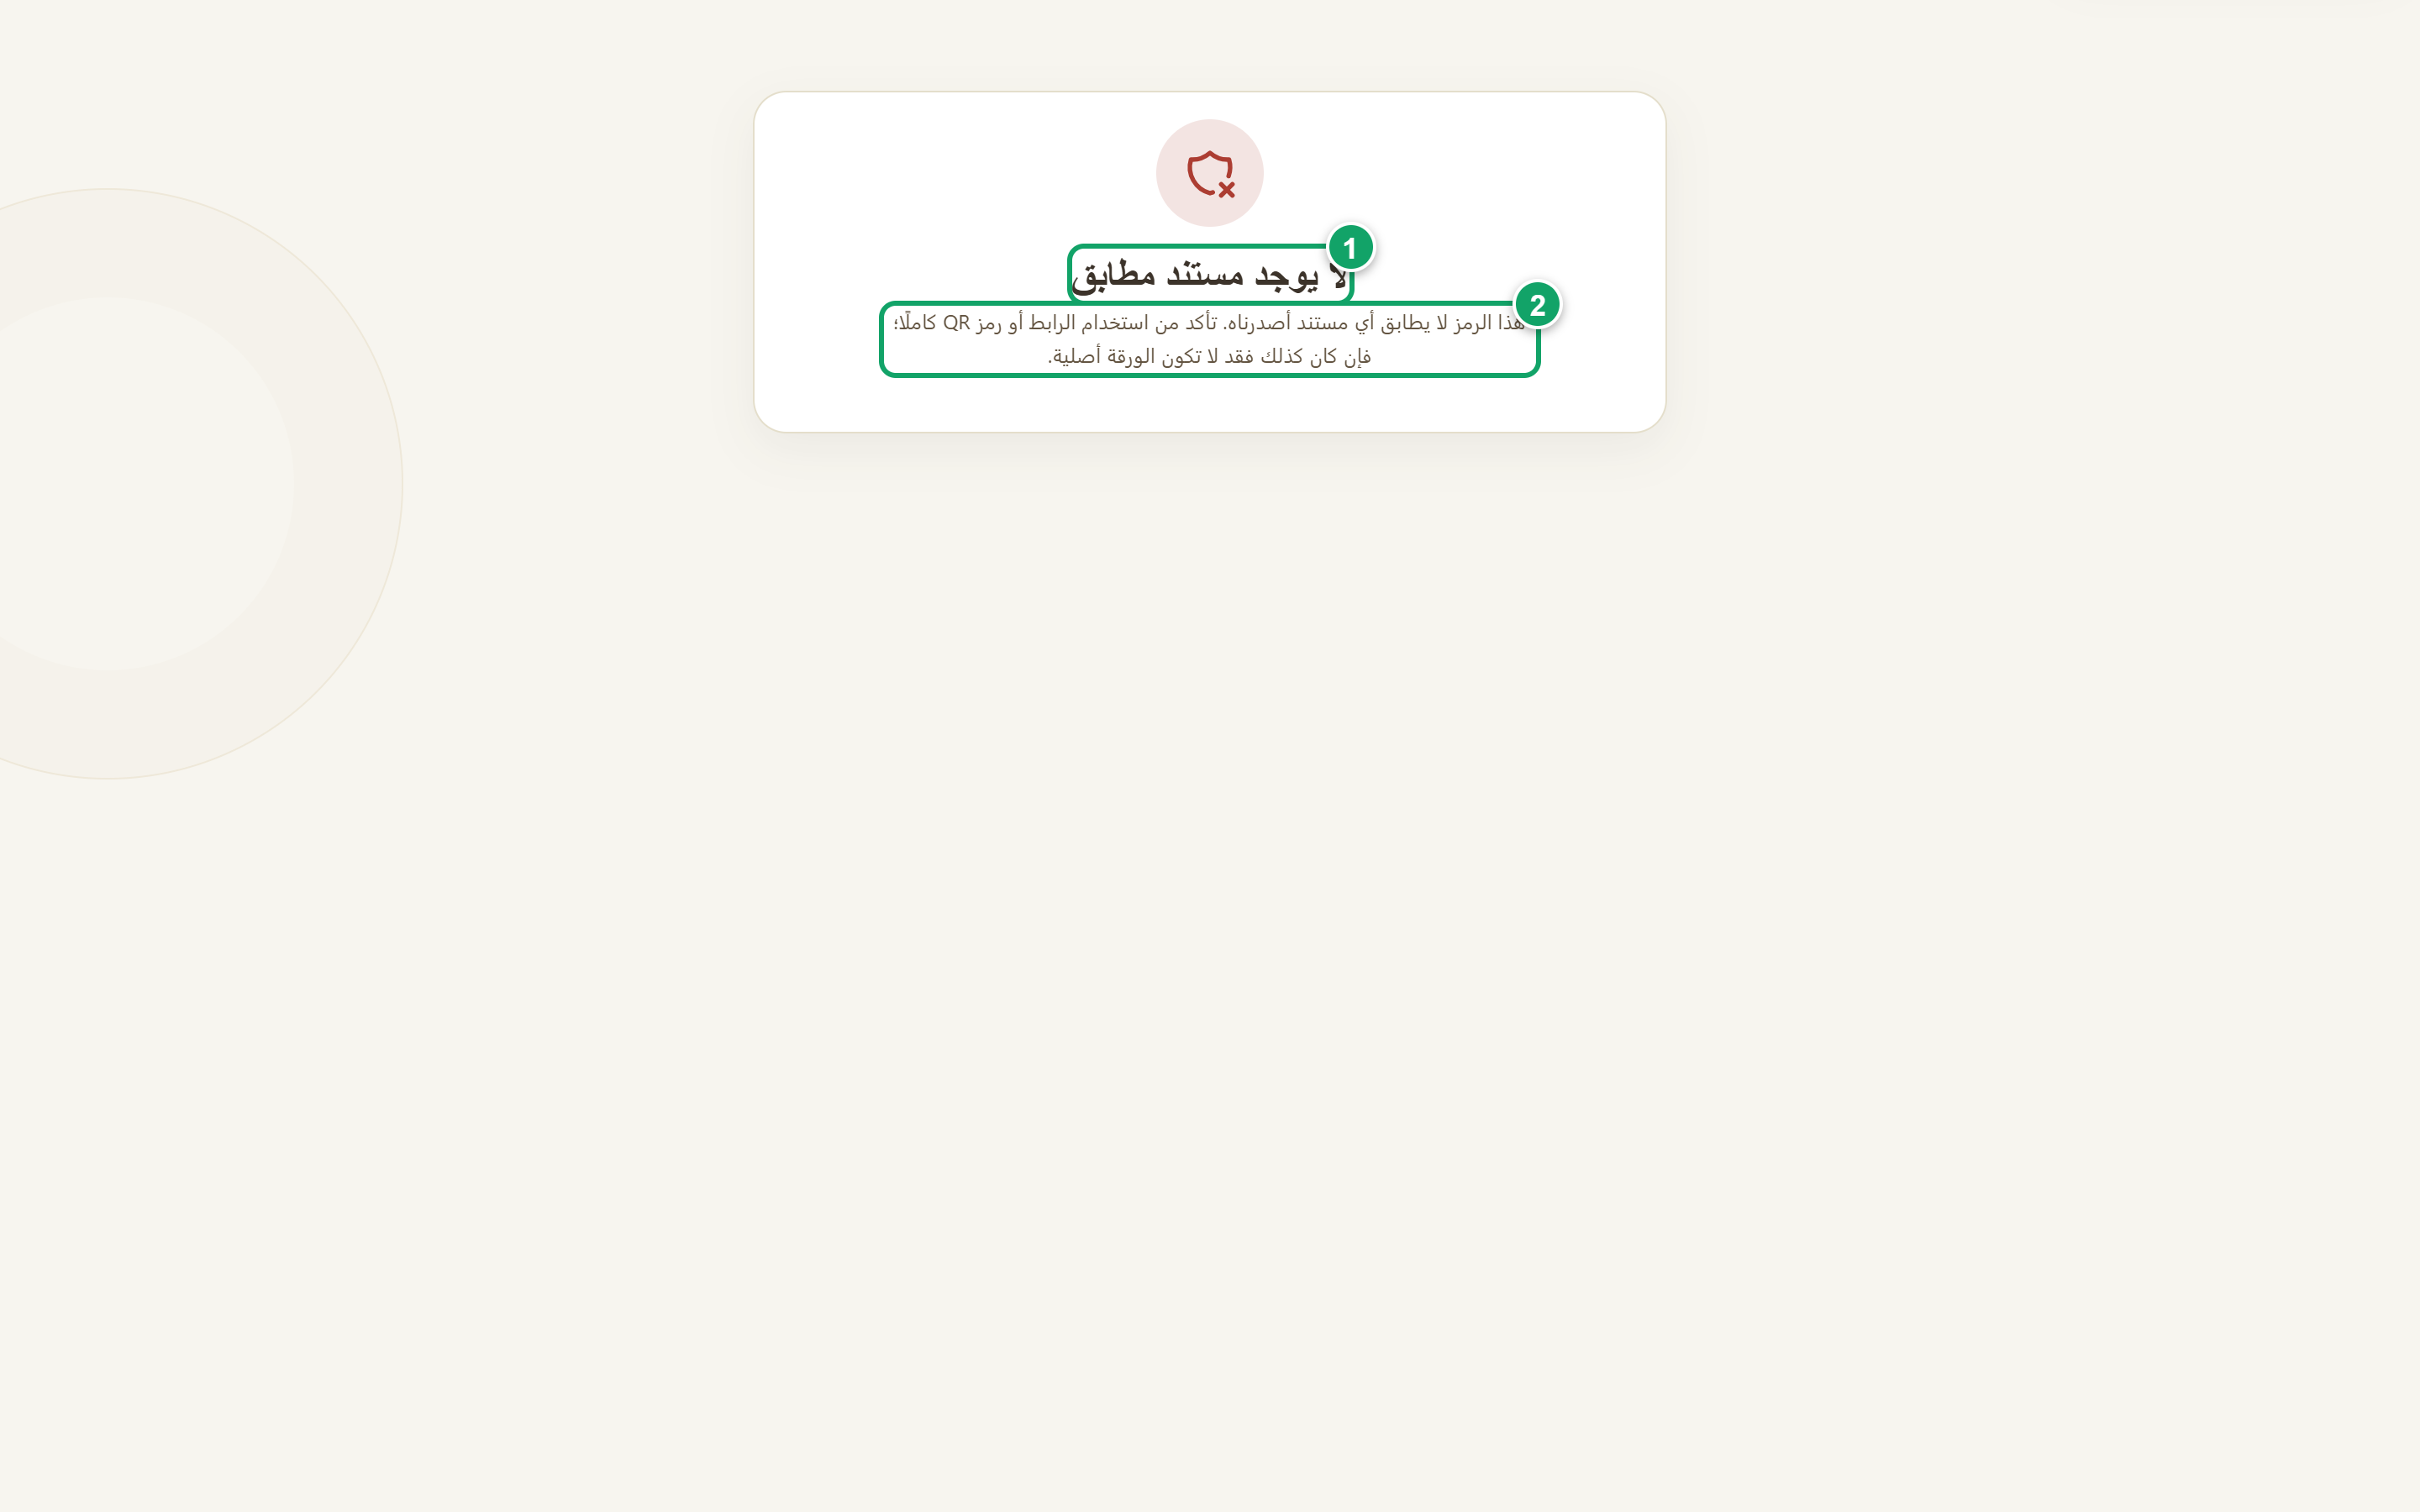
\includegraphics[width=0.95\linewidth,height=0.72\textheight,keepaspectratio]{figures/screens/ch06-print-verify-ar.png}
\caption{صفحة التحقق عند استخدام رمز غير صحيح}
\label{fig:builder-print-verify-screen}
\shotnote{تعرض الصورة صفحة التحقق العامة بعد فتحها برمز تجريبي لا يطابق أي مستند، لأن التقاطها برمز حقيقي يتطلب طباعة مستند فعلي. وهي النتيجة التي يراها من يحمل ورقة مزورة أو رابطاً منقوصاً، وتظهر دون تسجيل دخول. ① «لا يوجد مستند مطابق»: نتيجة الفحص. ② نص الإرشاد: يطلب التأكد من استخدام الرابط أو الرمز كاملاً قبل الحكم على الورقة.}
\end{figure}

\begin{table}[H]
\centering
\caption{ما تعرضه صفحة التحقق}
\label{tab:builder-print-verify-results}
\begin{tabularx}{\linewidth}{R{3.6cm} Y}
\rcHeaderRow
\thh{النتيجة} & \thh{معناها}\\
«الرمز موثّق» & صدر الرمز عن المؤسسة لهذا المستند. وتظهر «بيانات المستند»: «المستند» و«الجهة المُصدِرة» و«تاريخ الإصدار» و«إصدار القالب» و«بصمة الملف».\\
«المستند كما صدر» & نص المستند كما طُبع. وتظهر التواقيع مواضع تذكر اسم الموقّع، ولا يظهر رمز QR.\\
«تحقّق من ملف وصلك» & تختار ملف PDF أو Word وصلك، فيخبرك هل هو الملف نفسه الذي صدر. ويبقى الملف على جهازك.\\
«لا يوجد مستند مطابق» & الرمز لا يطابق أي مستند صادر، فتأكد من استخدام الرابط أو الرمز كاملاً، وإلا فقد لا تكون الورقة أصلية.\\
«تعذّر التحقق من هذا المستند الآن» & مشكلة مؤقتة لا تعني أن المستند غير أصلي، فأعد المحاولة بعد قليل.\\
\end{tabularx}
\end{table}

\begin{rcwarn}[قارن الورقة بالمستند المعروض]
إذا اختلف اسم أو رقم أو تاريخ أو مبلغ بين الورقة والمستند المعروض، فقد عُدّلت الورقة بعد إصدارها. وإذا طُبع المستند مع مستندات أخرى في ملف واحد بالطباعة الجماعية، فلا يمكن التحقق من ملفه، بل تقارن المحتوى فقط.
\end{rcwarn}

\begin{figure}[H]
\centering
\begin{tikzpicture}[node distance=0.5cm]
\node[stepBox] (a) {\RL{تفعيل رمز التحقق في المخرجات}};
\node[stepBox,below=of a] (b) {\RL{طباعة المستند برمز QR}};
\node[stepBox,below=of b] (c) {\RL{مسح الرمز}};
\node[stepBox,below=of c] (d) {\RL{مقارنة الورقة بالمستند كما صدر}};
\draw[flowsTo] (a) -- (b);
\draw[flowsTo] (b) -- (c);
\draw[flowsTo] (c) -- (d);
\end{tikzpicture}
\rclegend
\caption{من الطباعة إلى التحقق}
\label{fig:builder-print-verify-flow}
\shotnote{يبيّن المخطط أن التحقق يبدأ من قرار يتخذه مصمم القالب، فلا يحمل المستند رمزاً إذا لم يفعّله. وتنتهي الخطوات بالمقارنة لأن الصفحة تثبت ما صدر، ويبقى على القارئ أن يتأكد من أن الورقة تطابقه.}
\end{figure}

\subsection{خطوات العمل والتحقق}
\begin{enumerate}
\item فعّل «رمز QR يفتح صفحة تحقق» في «المخرجات»، وضع عنصر «رمز QR» في القالب أو في الترويسة.
\item انشر القالب، واطبع مستنداً تجريبياً من سجل.
\item امسح الرمز بهاتفك، وتأكد من ظهور «الرمز موثّق».
\item قارن «المستند كما صدر» بالورقة، وجرّب «تحقّق من ملف وصلك» بملف PDF الذي نزّلته.
\end{enumerate}

\textbf{تحقق ومعالجة المشكلة:} يجب أن تفتح الصفحة دون تسجيل دخول، وأن تطابق بياناتها الورقة. وإذا لم يُطبع الرمز على المستند، فالتحقق متوقف في هذا القالب، ففعّل «رمز QR يفتح صفحة تحقق» من «المخرجات». وإذا ظهر عند الطباعة «هذا المستند أكبر من أن يُتحقَّق منه برمز QR»، فأوقف التحقق في القالب أو اطبع صفوفاً أقل.

\clearpage
\section{الهويات والترويسات}
\label{sec:builder-feature-identities}

الهوية هي شعار المؤسسة واسمها وألوانها وبياناتها الرسمية، مثل السجل التجاري والعنوان. أما الترويسة فرأس الصفحة وتذييلها اللذان يظهران في المستندات المطبوعة. وتحفظهما هذه الصفحة في مكان واحد، فتستخدمهما قوالب الطباعة والمراسلات الرسمية معاً، وأي تغيير هنا يظهر فيها كلها في الطباعة التالية.

\textbf{المسار ومن يستخدمه:} «ادوات البناء» ← «الأساسية» ← «الهويات والترويسات». يستخدمها من يدير مظهر مستندات المؤسسة.

\begin{rcnote}[مثال: شركة الأفق]
يرفع مسؤول النظام شعار الأفق ويضيف بياناتها الرسمية إلى الهوية الافتراضية، ثم ينشئ ترويسة يظهر رأسها في الصفحة الأولى فقط، فتطبع ورقة الزيارة بشعار الشركة دون إعادة تصميمه في كل قالب. ويرفع الشعار في ③ ويحفظ من ④، ثم ينشئ الترويسة من ②.
\end{rcnote}

\begin{figure}[H]
\centering
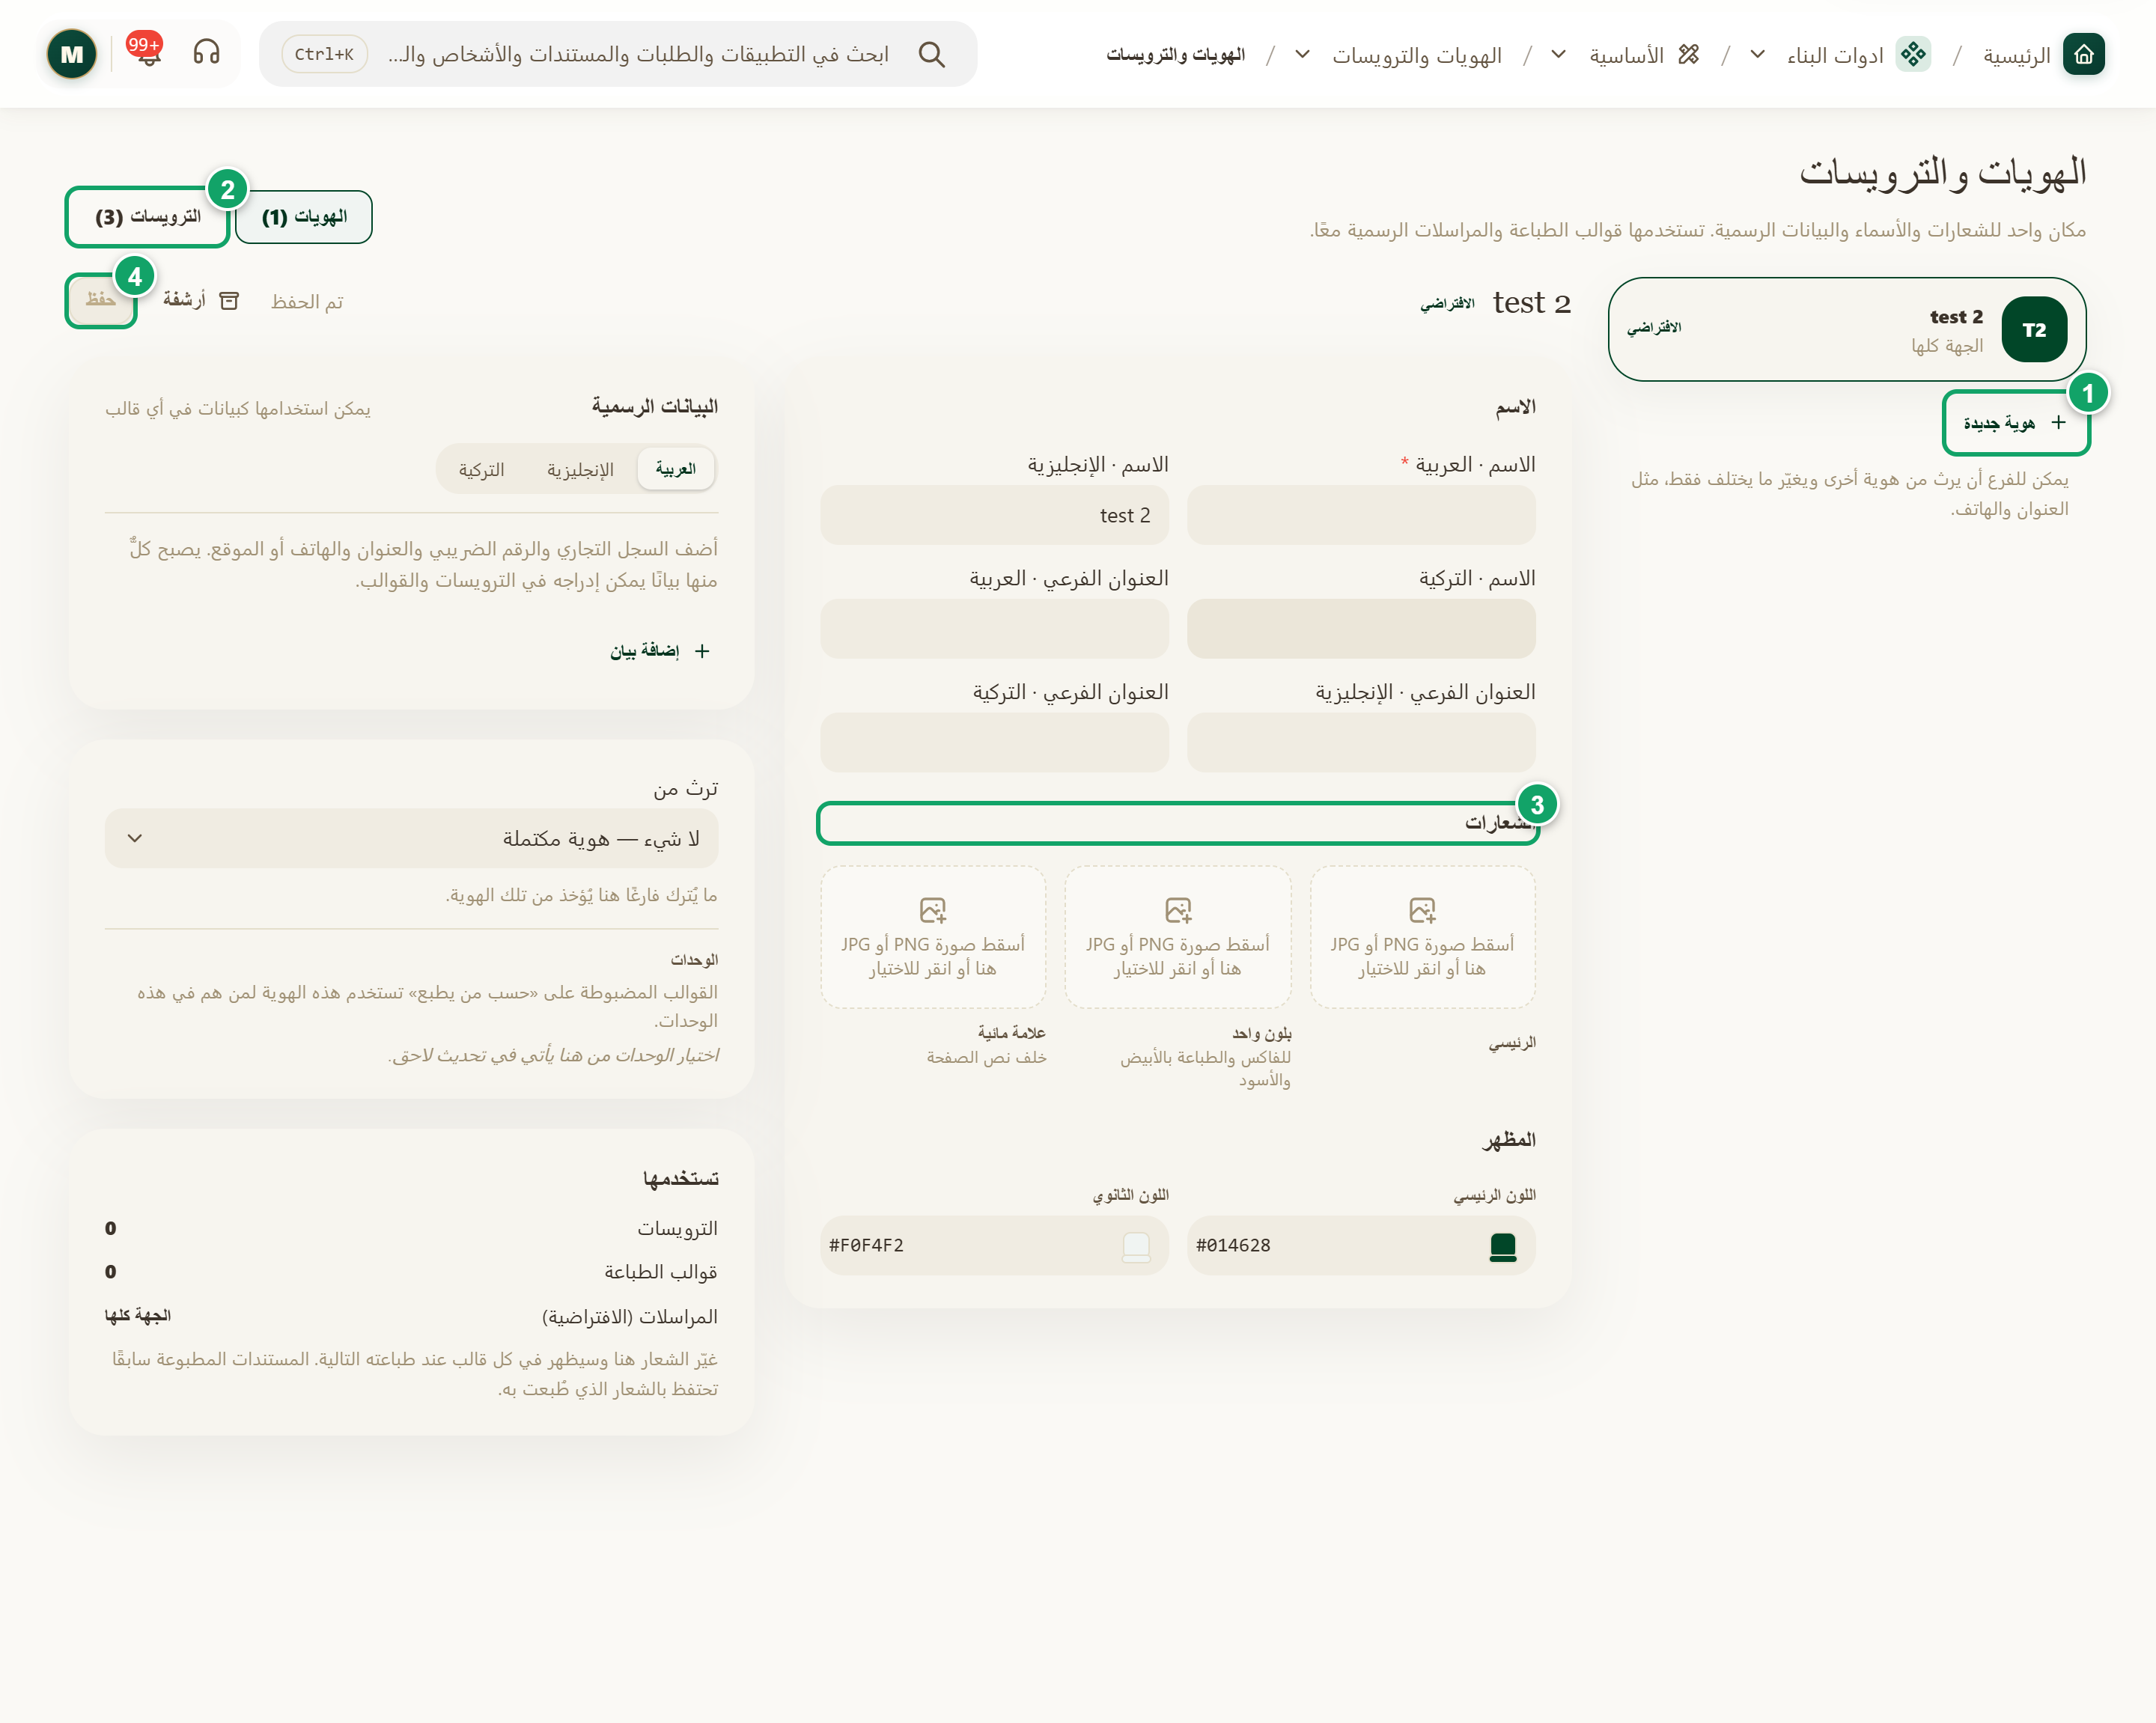
\includegraphics[width=0.95\linewidth,height=0.72\textheight,keepaspectratio]{figures/screens/ch06-identities-ar.png}
\caption{صفحة «الهويات والترويسات»}
\label{fig:builder-identities-screen}
\shotnote{تعرض الصفحة الهوية الافتراضية للمؤسسة وحقولها، وهي هنا هوية مؤسسة الاختبار. ① «هوية جديدة»: تنشئ هوية أخرى، مثل هوية فرع. ② «الترويسات»: تبويب الترويسات المشتركة. ③ «الشعارات»: الشعار الرئيسي وبلون واحد والعلامة المائية. ④ «حفظ»: يحفظ تعديل الهوية.}
\end{figure}


\begin{table}[H]
\centering
\caption{ما الذي تجده هنا؟}
\label{tab:builder-identities-data}
\begin{tabularx}{\linewidth}{R{3.6cm} Y}
\rcHeaderRow
\thh{الجزء} & \thh{المحتوى والإجراء}\\
الهويات & لكل هوية «الاسم» و«العنوان الفرعي» بكل لغة، و«الشعارات» (الرئيسي، بلون واحد، علامة مائية)، و«المظهر» بلونين، و«البيانات الرسمية».\\
ترث من & تجعل الهوية تأخذ ما لم تحدده من هوية أخرى، مثل هوية فرع ترث من هوية المؤسسة.\\
تستخدمها & تبيّن الترويسات وقوالب الطباعة والمراسلات التي تعتمد على الهوية.\\
الترويسات & قائمة الترويسات المشتركة، ولكل ترويسة عدد القوالب التي تستخدمها، ومنها «تعديل» و«نسخ» و«اجعله الافتراضي» و«أرشفة».\\
\end{tabularx}
\end{table}

\begin{figure}[H]
\centering
\begin{tikzpicture}[node distance=0.5cm]
\node[entity] (id) {\RL{الهوية}};
\node[entityOpt,below=0.7cm of id] (lh) {\RL{الترويسة}};
\node[entityOpt,below right=0.7cm and 0.3cm of lh] (print) {\RL{قوالب الطباعة}};
\node[entityOpt,below left=0.7cm and 0.3cm of lh] (corr) {\RL{المراسلات الرسمية}};
\draw[dependsOnOpt] (id) -- (lh);
\draw[dependsOnOpt] (lh.south) -- ++(0,-0.3) -| (print.north);
\draw[dependsOnOpt] (lh.south) -- ++(0,-0.3) -| (corr.north);
\end{tikzpicture}
\rclegend
\caption{من الهوية إلى المستند المطبوع}
\label{fig:builder-identities-model}
\shotnote{يوضّح الشكل أن الهوية تغذّي الترويسة، وأن الترويسة مشتركة بين قوالب الطباعة والمراسلات الرسمية. لذلك عدّل الشعار أو البيانات الرسمية في الهوية مرة واحدة، فيظهر التعديل في كل مستند يُطبع بعد ذلك؛ وراجع «تستخدمها» قبل أي تغيير.}
\end{figure}

\subsection{خطوات العمل والتحقق}
\begin{enumerate}
\item افتح «الهويات والترويسات»، واختر الهوية الافتراضية «الجهة كلها» أو أنشئ «هوية جديدة».
\item اكتب الاسم بكل لغة، وارفع الشعارات بصيغة PNG أو JPG، وأضف البيانات الرسمية، ثم اضغط «حفظ».
\item افتح «الترويسات»، وأنشئ «ترويسة جديدة»، واختر عناصرها ومكان ظهورها.
\end{enumerate}

\textbf{تحقق ومعالجة المشكلة:} اطبع مستنداً تجريبياً من قالب يستخدم الترويسة، فيجب أن يظهر الشعار والبيانات الجديدة. وإذا لم تستطع أرشفة هوية، فاجعل هوية أخرى هي الافتراضية أولاً، لأن الهوية الافتراضية لا تُؤرشف.

\clearpage
\section{محرر الترويسة}
\label{sec:builder-feature-letterheads}

الترويسة رأس صفحة وتذييل تصممهما مرة واحدة، فتستخدمهما قوالب الطباعة والمراسلات الرسمية. ويعرض محرر الترويسة ورقة فيها منطقتان: «الرأس» في أعلاها و«التذييل» في أسفلها، وبينهما مكان محتوى كل قالب. وتضيف إلى المنطقتين نصاً تكتبه بنفسك، أو بيانات من الهوية والمستند تتغير مع كل طباعة، مثل اسم الجهة وتاريخ الطباعة ورقم الصفحة. وأي تغيير تحفظه هنا يظهر في كل قالب يستخدم الترويسة وفي الخطابات الرسمية أيضاً.

\textbf{المسار ومن يستخدمه:} «ادوات البناء» ← «الأساسية» ← «الهويات والترويسات» ← «الترويسات» ← «ترويسة جديدة» أو «تعديل». يستخدمه من يدير مظهر مستندات المؤسسة.

\begin{rcnote}[مثال: شركة الأفق]
ينشئ مسؤول النظام ترويسة باسم «ترويسة الأفق»، ويضع في رأسها الشعار والاسم، وفي تذييلها عنوان المقر الرئيسي في دمشق ورقم الصفحة. ثم يجعل الرأس يظهر في الصفحة الأولى فقط والتذييل في كل صفحة، ويضغط «حفظ». فيكتب الاسم في ①، ويدرج الشعار من ② ورقم الصفحة من ③، ويحدد الصفحات بجانب ④، ثم يحفظ بـ ⑤.
\end{rcnote}

\begin{figure}[H]
\centering
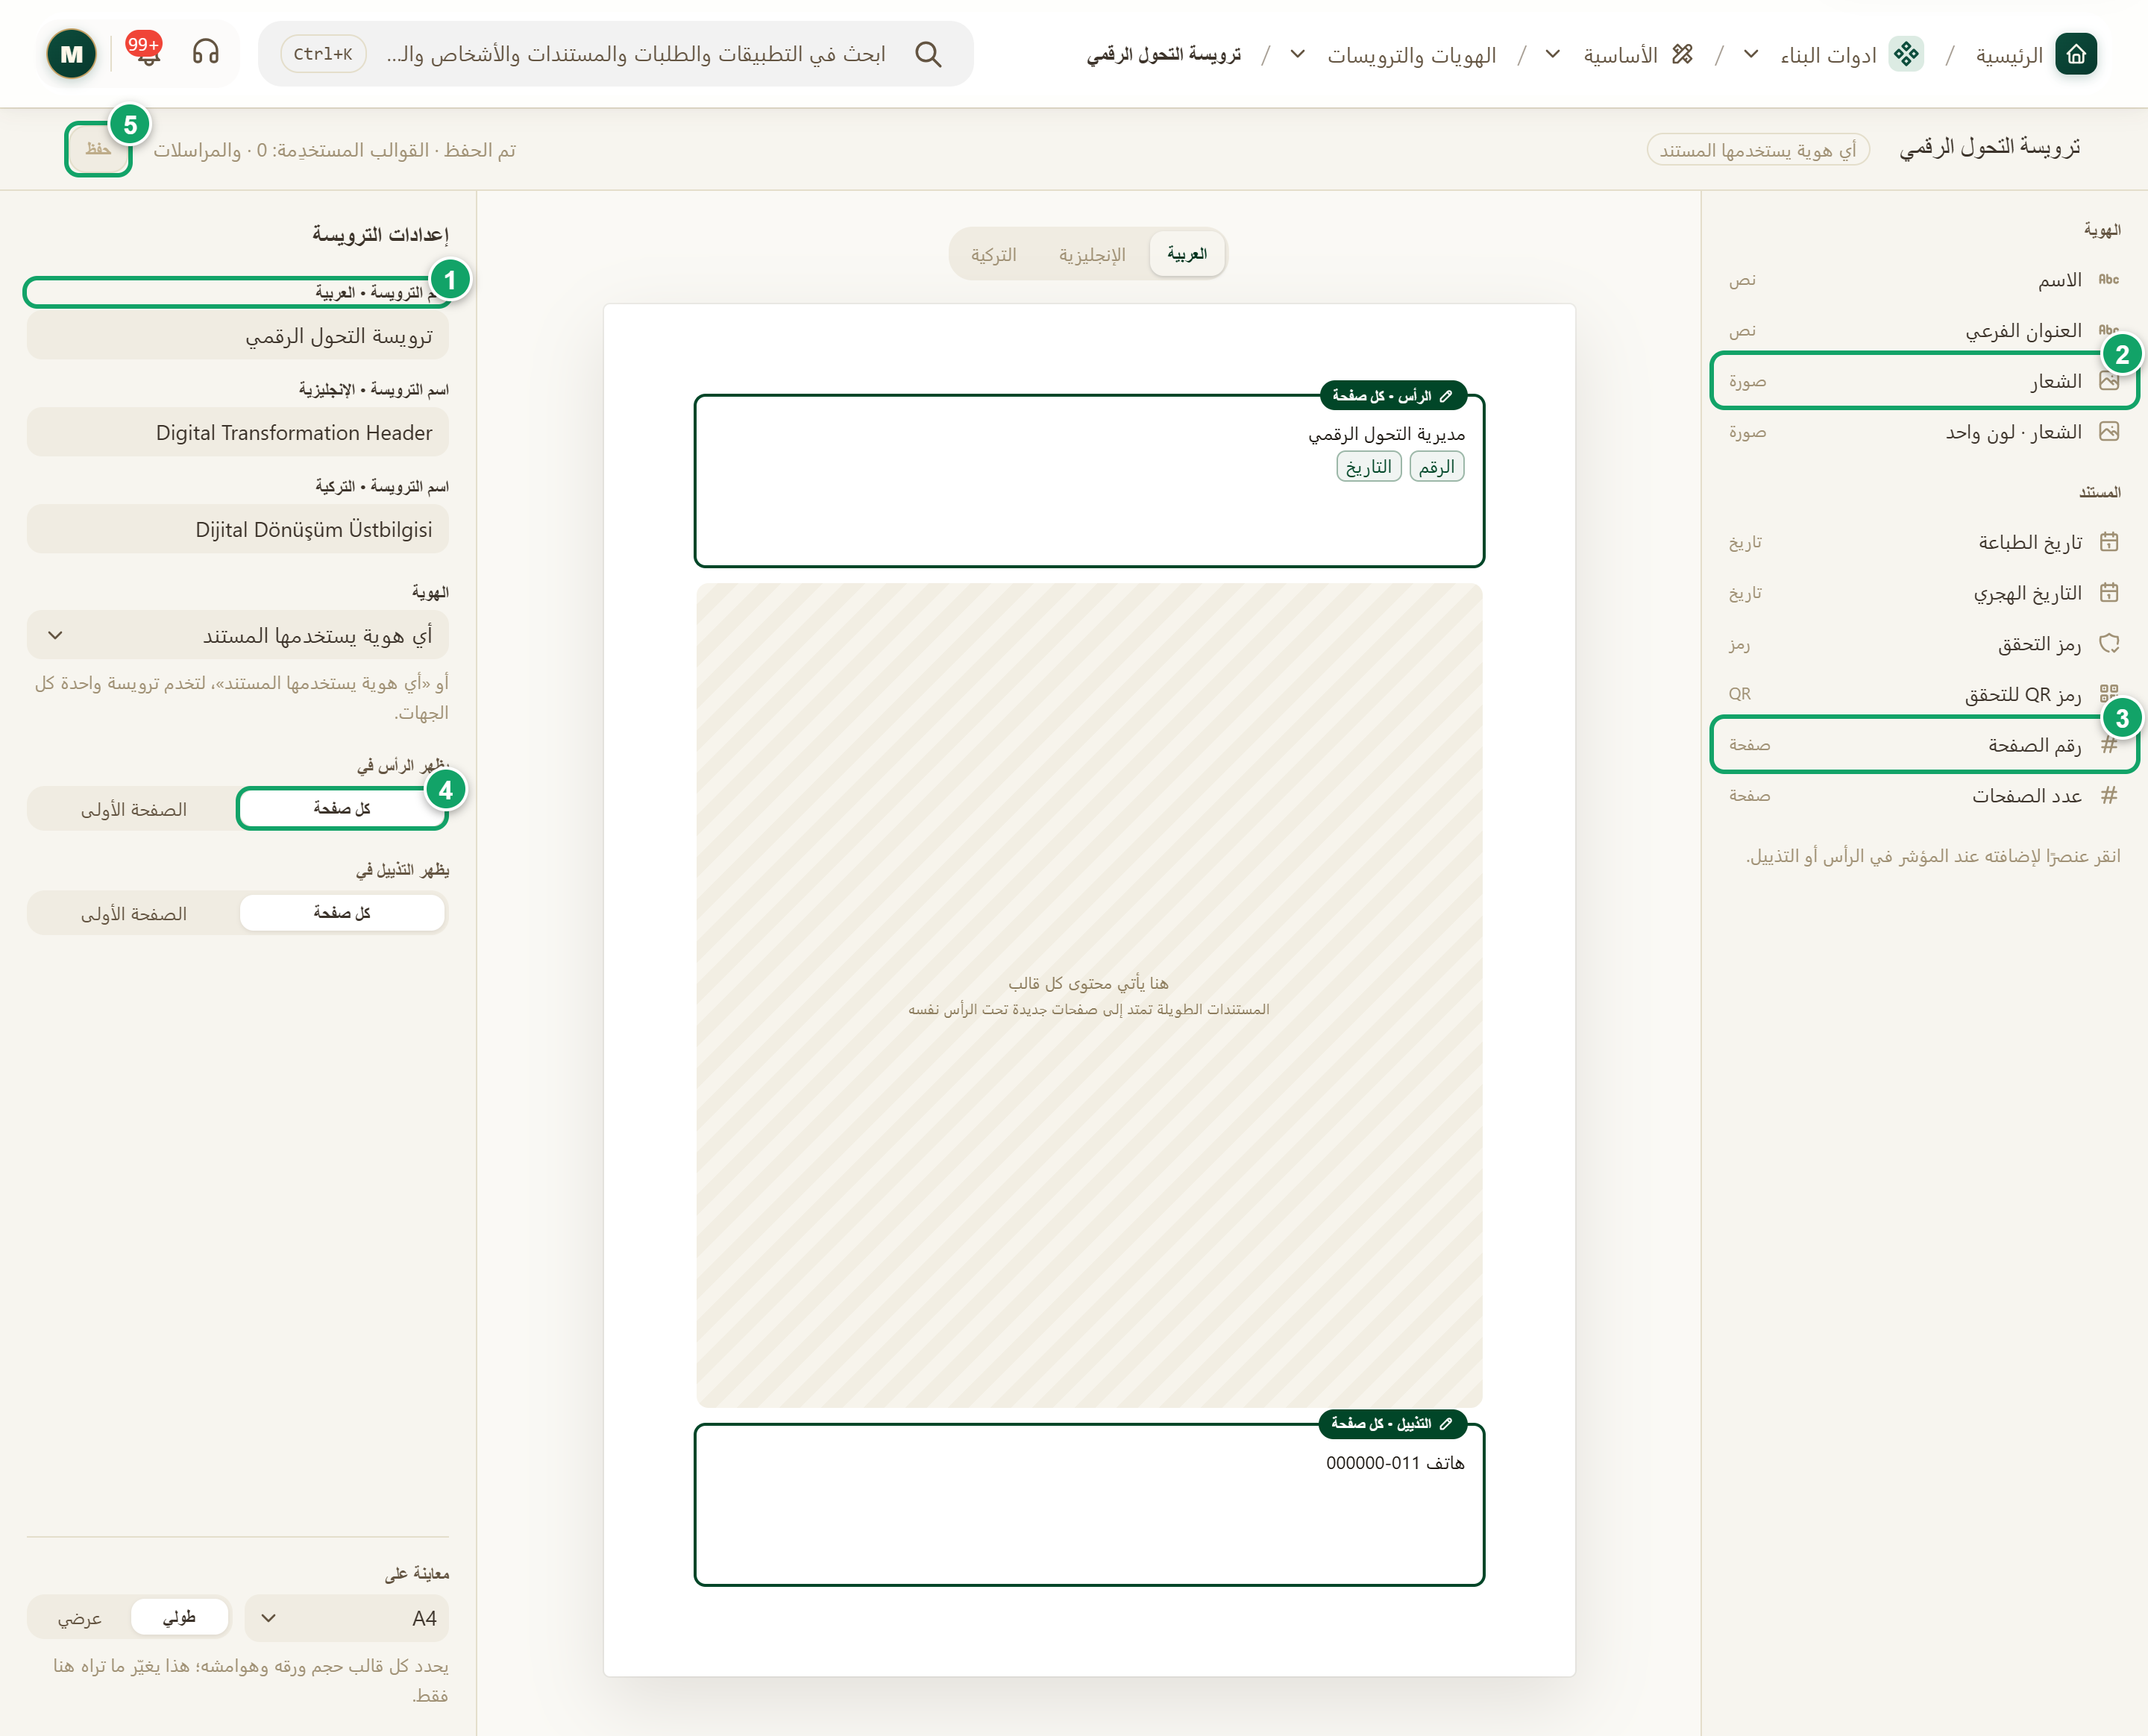
\includegraphics[width=0.95\linewidth,height=0.72\textheight,keepaspectratio]{figures/screens/ch06-letterheads-ar.png}
\caption{محرر الترويسة لترويسة موجودة}
\label{fig:builder-letterheads-screen}
\shotnote{تعرض الصورة ترويسة اختبارية في test2 مفتوحة في المحرر على اللغة العربية، وفي رأسها نص وعنصران من البيانات، وفي تذييلها رقم هاتف. ويبيّن السطر بجانب زر الحفظ عدد القوالب التي تستخدم الترويسة، فتعرف أثر أي تغيير قبل حفظه. ① «اسم الترويسة · العربية»: الاسم الذي يظهر عند اختيار الترويسة في القوالب. ② «الشعار»: يُدرَج من بيانات الهوية في موضع المؤشر. ③ «رقم الصفحة»: من بيانات المستند. ④ «كل صفحة»: الصفحات التي يظهر فيها الرأس. ⑤ «حفظ»: يحفظ الترويسة لكل من يستخدمها.}
\end{figure}

\begin{table}[H]
\centering
\caption{قائمة «البيانات» في المحرر}
\label{tab:builder-letterheads-data}
\begin{tabularx}{\linewidth}{R{3.6cm} Y}
\rcHeaderRow
\thh{المجموعة} & \thh{العناصر}\\
«الهوية» & «الاسم» و«العنوان الفرعي» و«الشعار» و«الشعار · لون واحد»، وكل بيان أضفته في «البيانات الرسمية» للهوية، مثل الرقم الضريبي.\\
«المستند» & «تاريخ الطباعة» و«التاريخ الهجري» و«رمز التحقق» و«رمز QR للتحقق» و«رقم الصفحة» و«عدد الصفحات».\\
\end{tabularx}
\end{table}

تضيف العنصر بالضغط عليه، فيُدرج في موضع المؤشر داخل الرأس أو التذييل.

\begin{table}[H]
\centering
\caption{«إعدادات الترويسة»}
\label{tab:builder-letterheads-settings}
\begin{tabularx}{\linewidth}{R{3.6cm} Y}
\rcHeaderRow
\thh{الإعداد} & \thh{ما يحدده}\\
«اسم الترويسة» & اسم يظهر عند اختيار الترويسة في القوالب، ويُكتب بكل لغة من لغات المؤسسة.\\
«الهوية» & هوية بعينها، أو «أي هوية يستخدمها المستند» لتخدم ترويسة واحدة كل الهويات.\\
«يظهر الرأس في» و«يظهر التذييل في» & «كل صفحة» أو «الصفحة الأولى».\\
«معاينة على» & «طولي» أو «عرضي»، وتغيّر ما تراه في المحرر فقط، لأن كل قالب يحدد ورقه وهوامشه بنفسه.\\
«لغة الترويسة» & تبويبات تظهر عندما يكون للمؤسسة أكثر من لغة، فتصمم نسخة الترويسة لكل لغة.\\
\end{tabularx}
\end{table}

\begin{figure}[H]
\centering
\begin{tikzpicture}[node distance=0.5cm]
\node[stepBox] (a) {\RL{ترويسة جديدة}};
\node[stepBox,below=of a] (b) {\RL{كتابة الرأس والتذييل}};
\node[stepBox,below=of b] (c) {\RL{إدراج بيانات الهوية والمستند}};
\node[stepBox,below=of c] (d) {\RL{ضبط الهوية والصفحات}};
\node[stepBox,below=of d] (e) {\RL{حفظ واختيارها في القوالب}};
\draw[flowsTo] (a) -- (b);
\draw[flowsTo] (b) -- (c);
\draw[flowsTo] (c) -- (d);
\draw[flowsTo] (d) -- (e);
\end{tikzpicture}
\rclegend
\caption{إعداد ترويسة مشتركة}
\label{fig:builder-letterheads-flow}
\shotnote{يبيّن المخطط أن الترويسة تُصمَّم مرة واحدة ثم تُختار في كل قالب، فلا تُعاد كتابتها في كل مستند. ويأتي إدراج بيانات الهوية بدلاً من كتابتها نصاً ثابتاً، لأن تغيير الشعار أو العنوان في الهوية يصل عندئذ إلى الترويسة تلقائياً.}
\end{figure}

\subsection{خطوات العمل والتحقق}
\begin{enumerate}
\item افتح «الهويات والترويسات»، ثم «الترويسات»، واضغط «ترويسة جديدة».
\item اكتب «اسم الترويسة»، واختر «الهوية» من «إعدادات الترويسة».
\item اضغط داخل الرأس، واكتب ما تريد، ثم أضف «الشعار» و«الاسم» من قائمة «البيانات».
\item اضغط داخل التذييل، وأضف العنوان أو بيانات التواصل و«رقم الصفحة».
\item اختر الصفحات التي يظهر فيها الرأس والتذييل، ثم اضغط «حفظ».
\end{enumerate}

\textbf{تحقق ومعالجة المشكلة:} يجب أن تتحول الحالة إلى «تم الحفظ» مع عدد القوالب التي تستخدم الترويسة، وأن تظهر الترويسة في قائمة الترويسات. فإذا ظهر «أدخل اسمًا للترويسة.»، فاكتب الاسم ثم احفظ. وإذا ظهر عند الأرشفة «ما زالت قوالب طباعة تستخدم هذه الترويسة»، فاختر ترويسة أخرى في تلك القوالب أولاً.


\chapter{لوحات المعلومات والتقارير}
\label{ch:builder-dashboards}

\section{ماذا ستبني في هذا الفصل؟}
\label{sec:builder-dashboards-intro}

بعد أن تتراكم السجلات يحتاج المديرون إلى أرقام تلخّص العمل، مثل عدد الطلبات المفتوحة أو المتأخرة. ويشرح هذا الفصل بناء لوحة المعلومات من أولها إلى عرضها: تنشئها في القائمة، ثم تضيف إليها الأقسام والعناصر وتربط كل عنصر بمصدر بياناته، وتضبط إعداداتها ومرشحاتها، ثم تعاينها وتنشرها. ويشرح بعد ذلك كيف يعرضها الفريق ويصدّرها، وكيف تُنشر لوحات الذكاء الاصطناعي صفحاتٍ في التطبيقات، وكيف تطرح أسئلة سريعة في تقارير الذكاء الاصطناعي.

ويرى كل مشاهد في اللوحة ما تسمح به صلاحياته ما لم يختر صاحبها غير ذلك صراحة، لذلك تتكرر في الصفحات مراجعة مستوى الوصول قبل النشر.

\begin{rcnote}[مثال: شركة الأفق]
يبني مسؤول النظام في الأفق لوحة «متابعة الزيارات» تعرض طلبات الزيارة في كل حالة وفي كل فرع، ثم ينشرها في تطبيق «خدمات الفروع»، فتراجع سارة الخطيب كل صباح الطلبات التي تنتظر قرارها.
\end{rcnote}

\section{صفحات هذا الفصل}
\label{sec:builder-dashboards-pages}

تبدأ أربع صفحات من قسم «الأساسية» في أدوات البناء: «لوحات المعلومات» و«الصفحات» و«لوحات معلومات الذكاء الاصطناعي» و«تقارير الذكاء الاصطناعي». أما الصفحات الثماني بينها فتشرح منشئ اللوحة الذي تفتحه من بطاقة اللوحة، ثم عرض اللوحة المنشورة. واتبع الترتيب في المرة الأولى، لأن كل صفحة تبني على ما قبلها.

\begin{table}[H]
\centering
\caption{التقارير والمتابعة}
\label{tab:builder-pages-reports}
\rcZebra
\begin{tabularx}{\linewidth}{R{4.2cm} Y}
\rcHeaderRow
\thh{الصفحة وقسمها} & \thh{ماذا تقدم هذه الصفحة؟}\\
لوحات المعلومات — الأساسية & تنشئ اللوحات وترتّبها في مجلدات وتحدد من يصل إلى كل منها.\\
منشئ اللوحة: الأقسام والعناصر — منشئ اللوحة & تضيف الأقسام والعناصر وترتّبها في الشبكة وتحفظ المسودة.\\
إعدادات العنصر ومصادر بياناته — منشئ اللوحة & تختار مصدر أرقام العنصر وطريقة حسابها ومستوى الوصول ومظهره.\\
أنواع العناصر — منشئ اللوحة & تعرّف بالعناصر والرسوم البيانية المتاحة ومتى تستخدم كلاً منها.\\
إعدادات اللوحة — منشئ اللوحة & تحدد اسم اللوحة ومكانها في التنقل والبيانات التي يراها المشاهد.\\
مرشحات المشاهد ومحددات الكيانات — منشئ اللوحة & تضيف مرشحات التاريخ والسجلات والخيارات التي يغيّرها المشاهد.\\
منشئ اللوحة بالذكاء الاصطناعي — منشئ اللوحة & تصف اللوحة بكلماتك فيقترح الذكاء الاصطناعي عناصرها لتراجعها.\\
المعاينة والنشر والإصدارات — منشئ اللوحة & تعاين اللوحة وتنشرها وتعود إلى إصدار سابق عند الحاجة.\\
عرض اللوحة وتصديرها — عرض اللوحة & يغيّر المشاهد المرشحات ويصدّر بيانات جدول أو تقرير \en{PDF}.\\
الصفحات — الأساسية & تنشر لوحات الذكاء الاصطناعي صفحاتٍ مستقلة داخل التطبيقات.\\
لوحات معلومات الذكاء الاصطناعي — الأساسية & تبني لوحات معلومات بمساعدة الذكاء الاصطناعي في مساحة خاصة بك.\\
تقارير الذكاء الاصطناعي — الأساسية & تجيب عن أسئلتك عن بيانات المؤسسة بتقرير مكتوب.\\
\end{tabularx}
\end{table}

\clearpage
\section{لوحات المعلومات}
\label{sec:builder-feature-dashboards}

لوحة المعلومات صفحة أرقام ورسوم بيانية تلخّص العمل، مثل عدد الطلبات المفتوحة أو المتأخرة. وتبدأ كل لوحة من صفحة «لوحات المعلومات»، وفيها تُنشئ اللوحات وترتّبها في مجلدات وتحدد من يصل إلى كل منها. أما بناء محتوى اللوحة فيجري في منشئ اللوحة الذي تشرحه الصفحات التالية.

\textbf{المسار ومن يستخدمه:} «ادوات البناء» ← «الأساسية» ← «لوحات المعلومات». يظهر زر «إنشاء لوحة معلومات» لمن يملك صلاحية إنشاء اللوحات، ويرى كل مستخدم البطاقات التي يملك صلاحية فتحها.

\begin{rcnote}[مثال: شركة الأفق]
ينشئ مسؤول النظام مجلداً باسم «خدمات الفروع»، ثم ينشئ داخله لوحة «متابعة الزيارات» ويمنح دور سارة الخطيب الوصول إليها. وتبدأ اللوحة من ①، ويبدأ المجلد من ②.
\end{rcnote}

\begin{figure}[H]
\centering
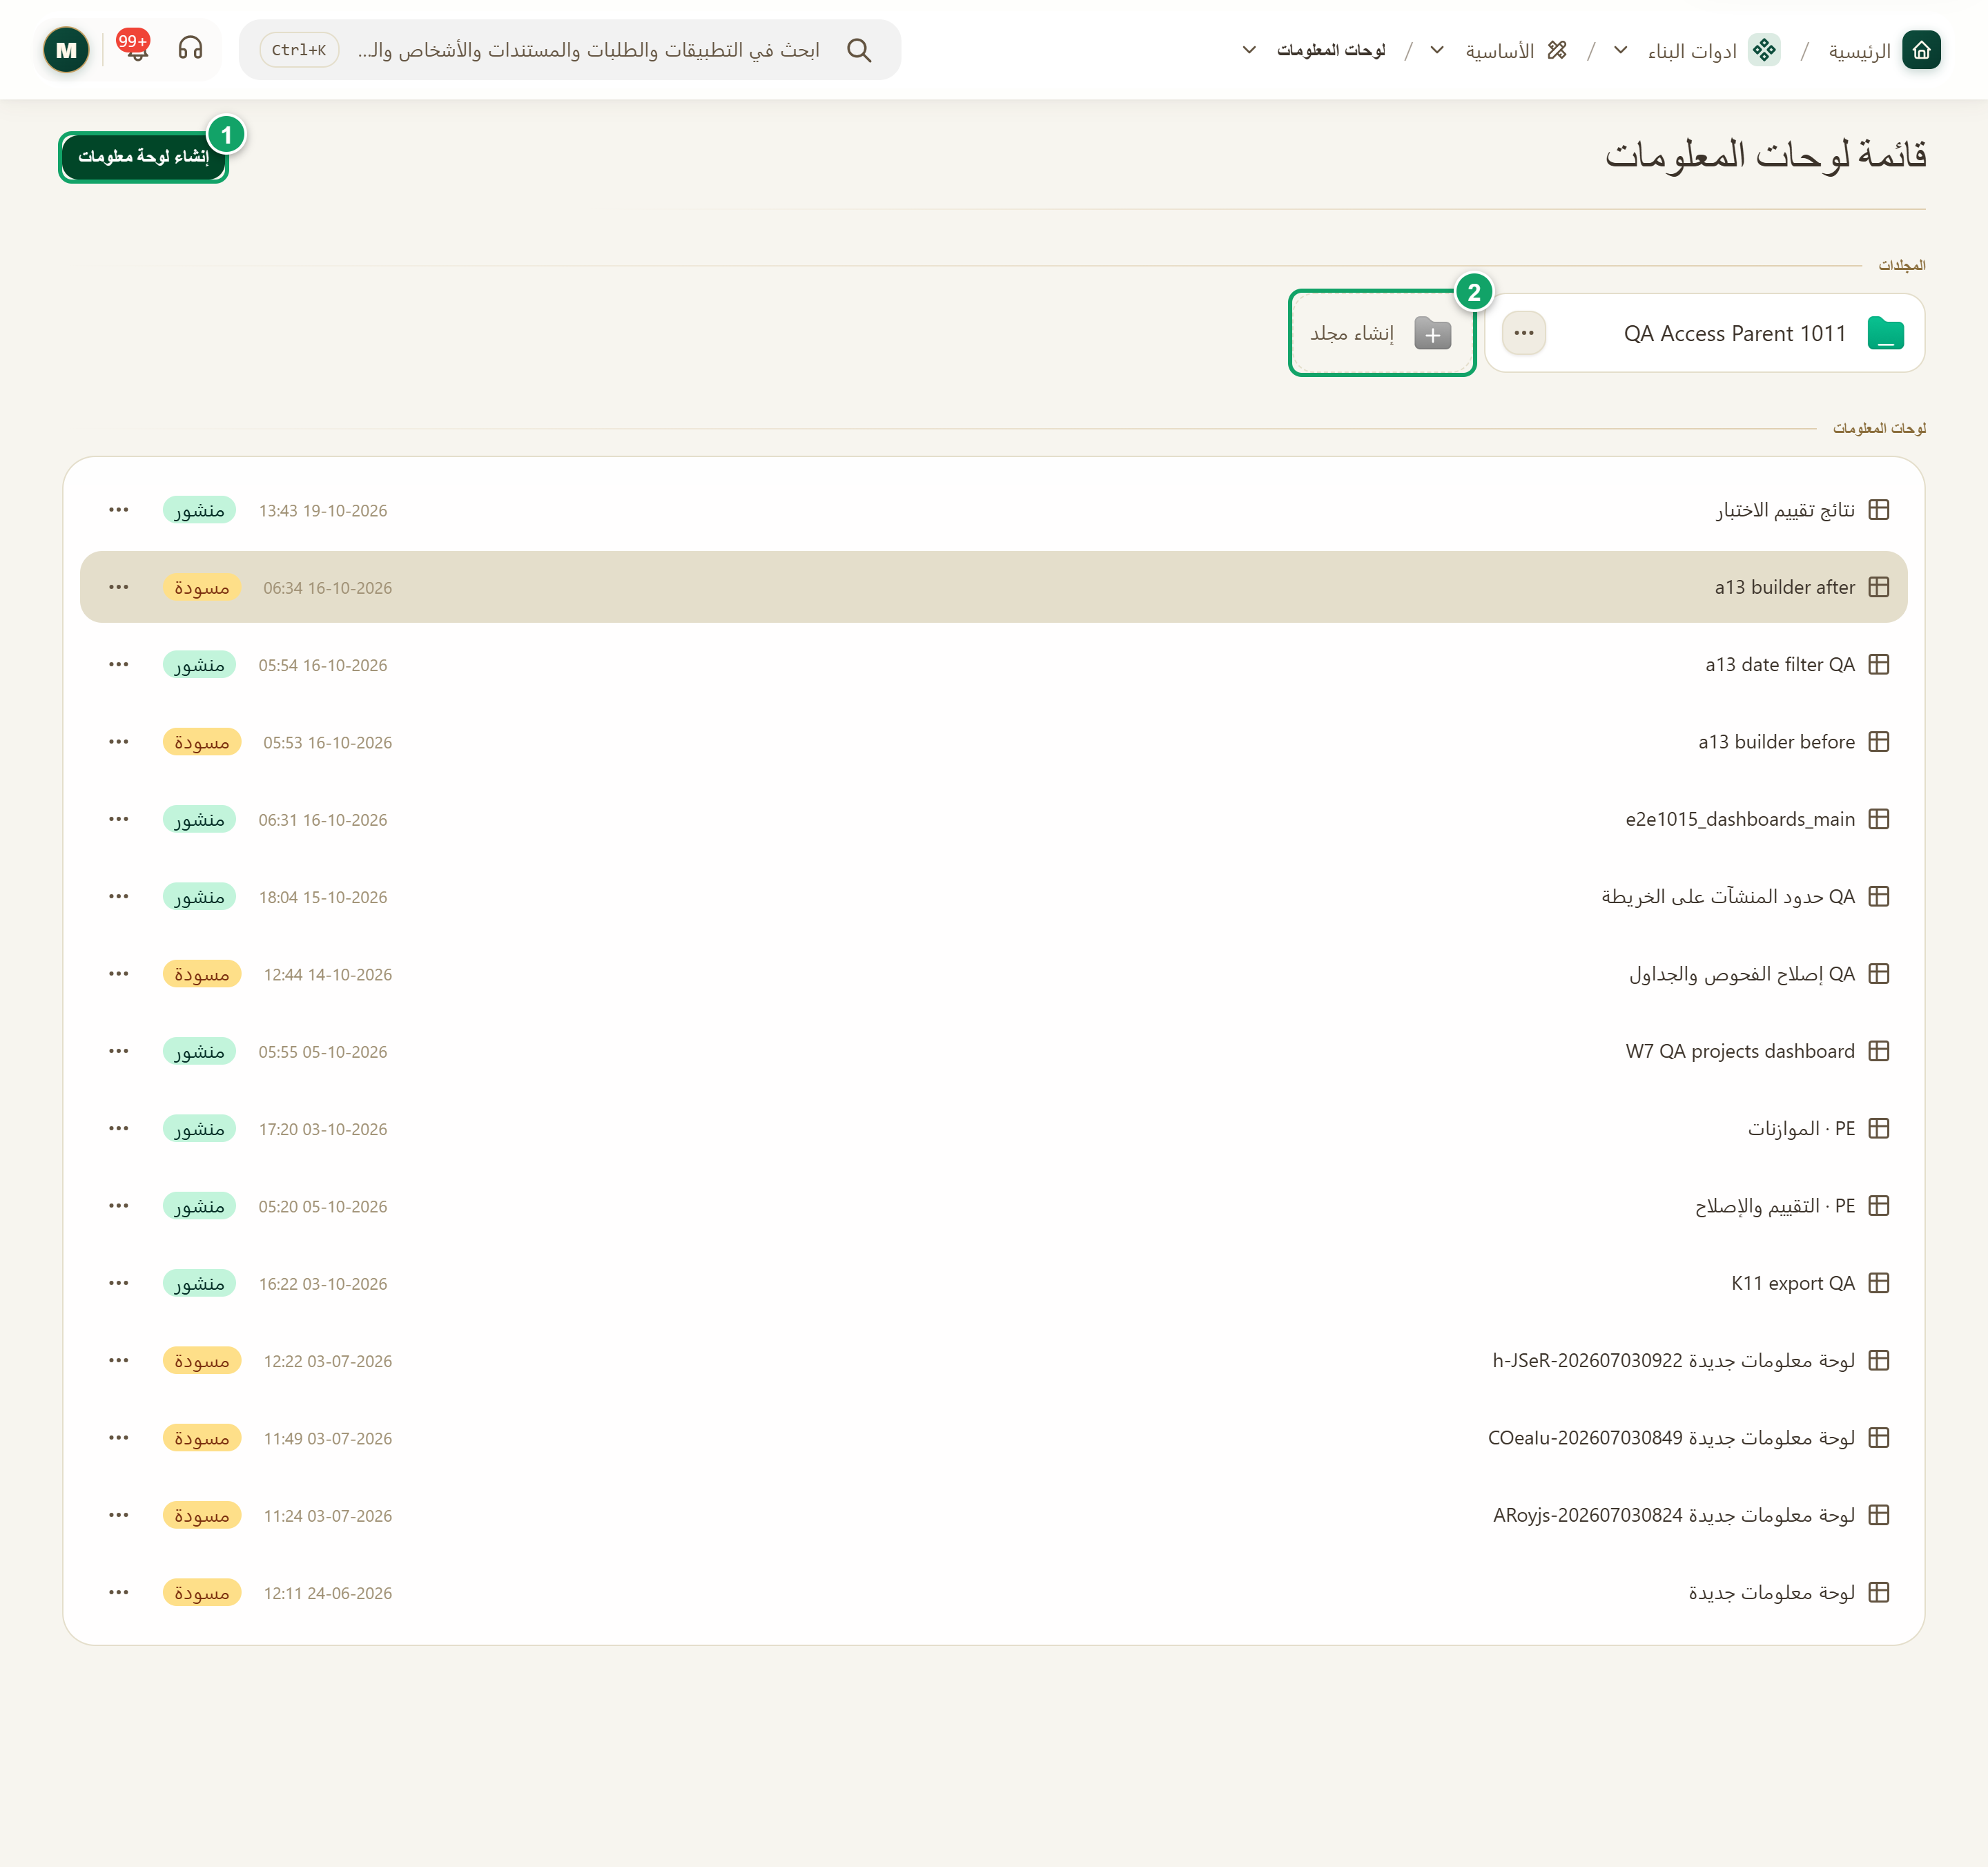
\includegraphics[width=0.95\linewidth,height=0.72\textheight,keepaspectratio]{figures/screens/ch06-dashboards-ar.png}
\caption{صفحة «لوحات المعلومات»}
\label{fig:builder-dashboards-screen}
\shotnote{تعرض الصفحة المجلدات ولوحات المعلومات مع حالتها، وهي هنا لوحات اختبار. ① «إنشاء لوحة معلومات»: تبدأ لوحة جديدة. ② «إنشاء مجلد»: ينظّم اللوحات في مجلدات.}
\end{figure}


\begin{table}[H]
\centering
\caption{ما الذي تجده في القائمة؟}
\label{tab:builder-dashboards-data}
\begin{tabularx}{\linewidth}{R{3.6cm} Y}
\rcHeaderRow
\thh{الجزء} & \thh{المحتوى والإجراء}\\
بطاقة اللوحة & تعرض اسم اللوحة وآخر تعديل عليها وحالتها: «مسودة» إذا لم تُنشر بعد، أو «منشور». وتفتح قائمتها الإجراءات «عرض» و«تعديل» و«إدارة الصلاحيات» و«حذف» بحسب صلاحياتك.\\
«إنشاء لوحة معلومات» & تطلب «اسم لوحة المعلومات» ووصفاً لا يقل عن اثني عشر حرفاً وكلمتين، ثم تفتح اللوحة الجديدة في المنشئ. وتُنشأ اللوحة داخل المجلد المفتوح.\\
المجلدات & «إنشاء مجلد» ينشئ مجلداً يضم لوحات ومجلدات فرعية. وتنقل اللوحة إليه بسحب بطاقتها وإفلاتها فوقه، وتُنقل محتويات المجلد إلى خارجه عند حذفه.\\
الوصول & يحدد «إدارة الوصول» الأدوار والأشخاص الذين يفتحون اللوحة. وتحصل اللوحة أيضاً على الوصول الممنوح لمجلدها، فإزالة شخص من اللوحة لا تزيل وصوله من المجلد.\\
\end{tabularx}
\end{table}

\begin{figure}[H]
\centering
\begin{tikzpicture}[node distance=0.5cm]
\node[stepBox] (a) {\RL{إنشاء مجلد عند الحاجة}};
\node[stepBox,below=of a] (b) {\RL{إنشاء لوحة معلومات داخله}};
\node[stepBox,below=of b] (c) {\RL{البناء والنشر في المنشئ}};
\node[stepBox,below=of c] (d) {\RL{منح الوصول للأدوار}};
\draw[flowsTo] (a) -- (b);
\draw[flowsTo] (b) -- (c);
\draw[flowsTo] (c) -- (d);
\end{tikzpicture}
\rclegend
\caption{من القائمة إلى لوحة يصل إليها الفريق}
\label{fig:builder-dashboards-flow}
\shotnote{يبيّن المخطط أن مكان اللوحة يُحدَّد قبل إنشائها، لأنها تُنشأ داخل المجلد المفتوح وترث الوصول الممنوح له. ويأتي منح الوصول بعد النشر، لأن من يفتح لوحة غير منشورة يرى رسالة تفيد بأنها لم تُنشر بعد.}
\end{figure}

\subsection{خطوات العمل والتحقق}
\begin{enumerate}
\item افتح «لوحات المعلومات»، واضغط «إنشاء مجلد» إذا أردت تجميع لوحات قسم واحد، ثم افتح المجلد.
\item اضغط «إنشاء لوحة معلومات»، واكتب «اسم لوحة المعلومات» ووصفاً يشرح ما تتابعه اللوحة، ثم اضغط «إنشاء».
\item ابنِ اللوحة وانشرها كما في الصفحات التالية، ثم عُد إلى القائمة وتأكد أن حالتها «منشور».
\item اختر «إدارة الصلاحيات» من قائمة البطاقة، وأضف الأدوار التي يجب أن تراها.
\end{enumerate}

\textbf{تحقق ومعالجة المشكلة:} يجب أن تظهر البطاقة في المجلد الصحيح بحالة «منشور»، وأن يفتحها المستخدم المقصود. فإذا ظهرت رسالة «صِف في 12 حرفاً وكلمتين على الأقل»، فأطل الوصف. وإذا بقي شخص يرى اللوحة بعد إزالته، فراجع الوصول الممنوح على مجلدها.

\clearpage
\section{منشئ اللوحة: الأقسام والعناصر}
\label{sec:builder-feature-dashboards-builder}

منشئ اللوحة هو المكان الذي تبني فيه محتوى اللوحة. وتتكون اللوحة من أقسام متتالية، لكل قسم عنوان ووصف وشبكة تضع فيها العناصر، والعنصر هو رقم أو رسم بياني أو جدول أو غير ذلك. وتُحفظ تعديلاتك مسودةً بزر «حفظ»، ولا يراها المشاهدون حتى تنشرها.

\textbf{المسار ومن يستخدمه:} «لوحات المعلومات» ← قائمة بطاقة اللوحة ← «تعديل». يستخدمه من يملك صلاحية تعديل اللوحة، ويُفتح تلقائياً بعد إنشاء لوحة جديدة.

\begin{rcnote}[مثال: شركة الأفق]
يضيف مسؤول النظام إلى لوحة «متابعة الزيارات» قسماً بعنوان «حالة الطلبات» فيه رقم للطلبات المنتظرة ورسم دائري للطلبات حسب الحالة، ثم قسماً ثانياً بعنوان «المواعيد» فيه تقويم الزيارات.
\end{rcnote}

\begin{figure}[H]
\centering
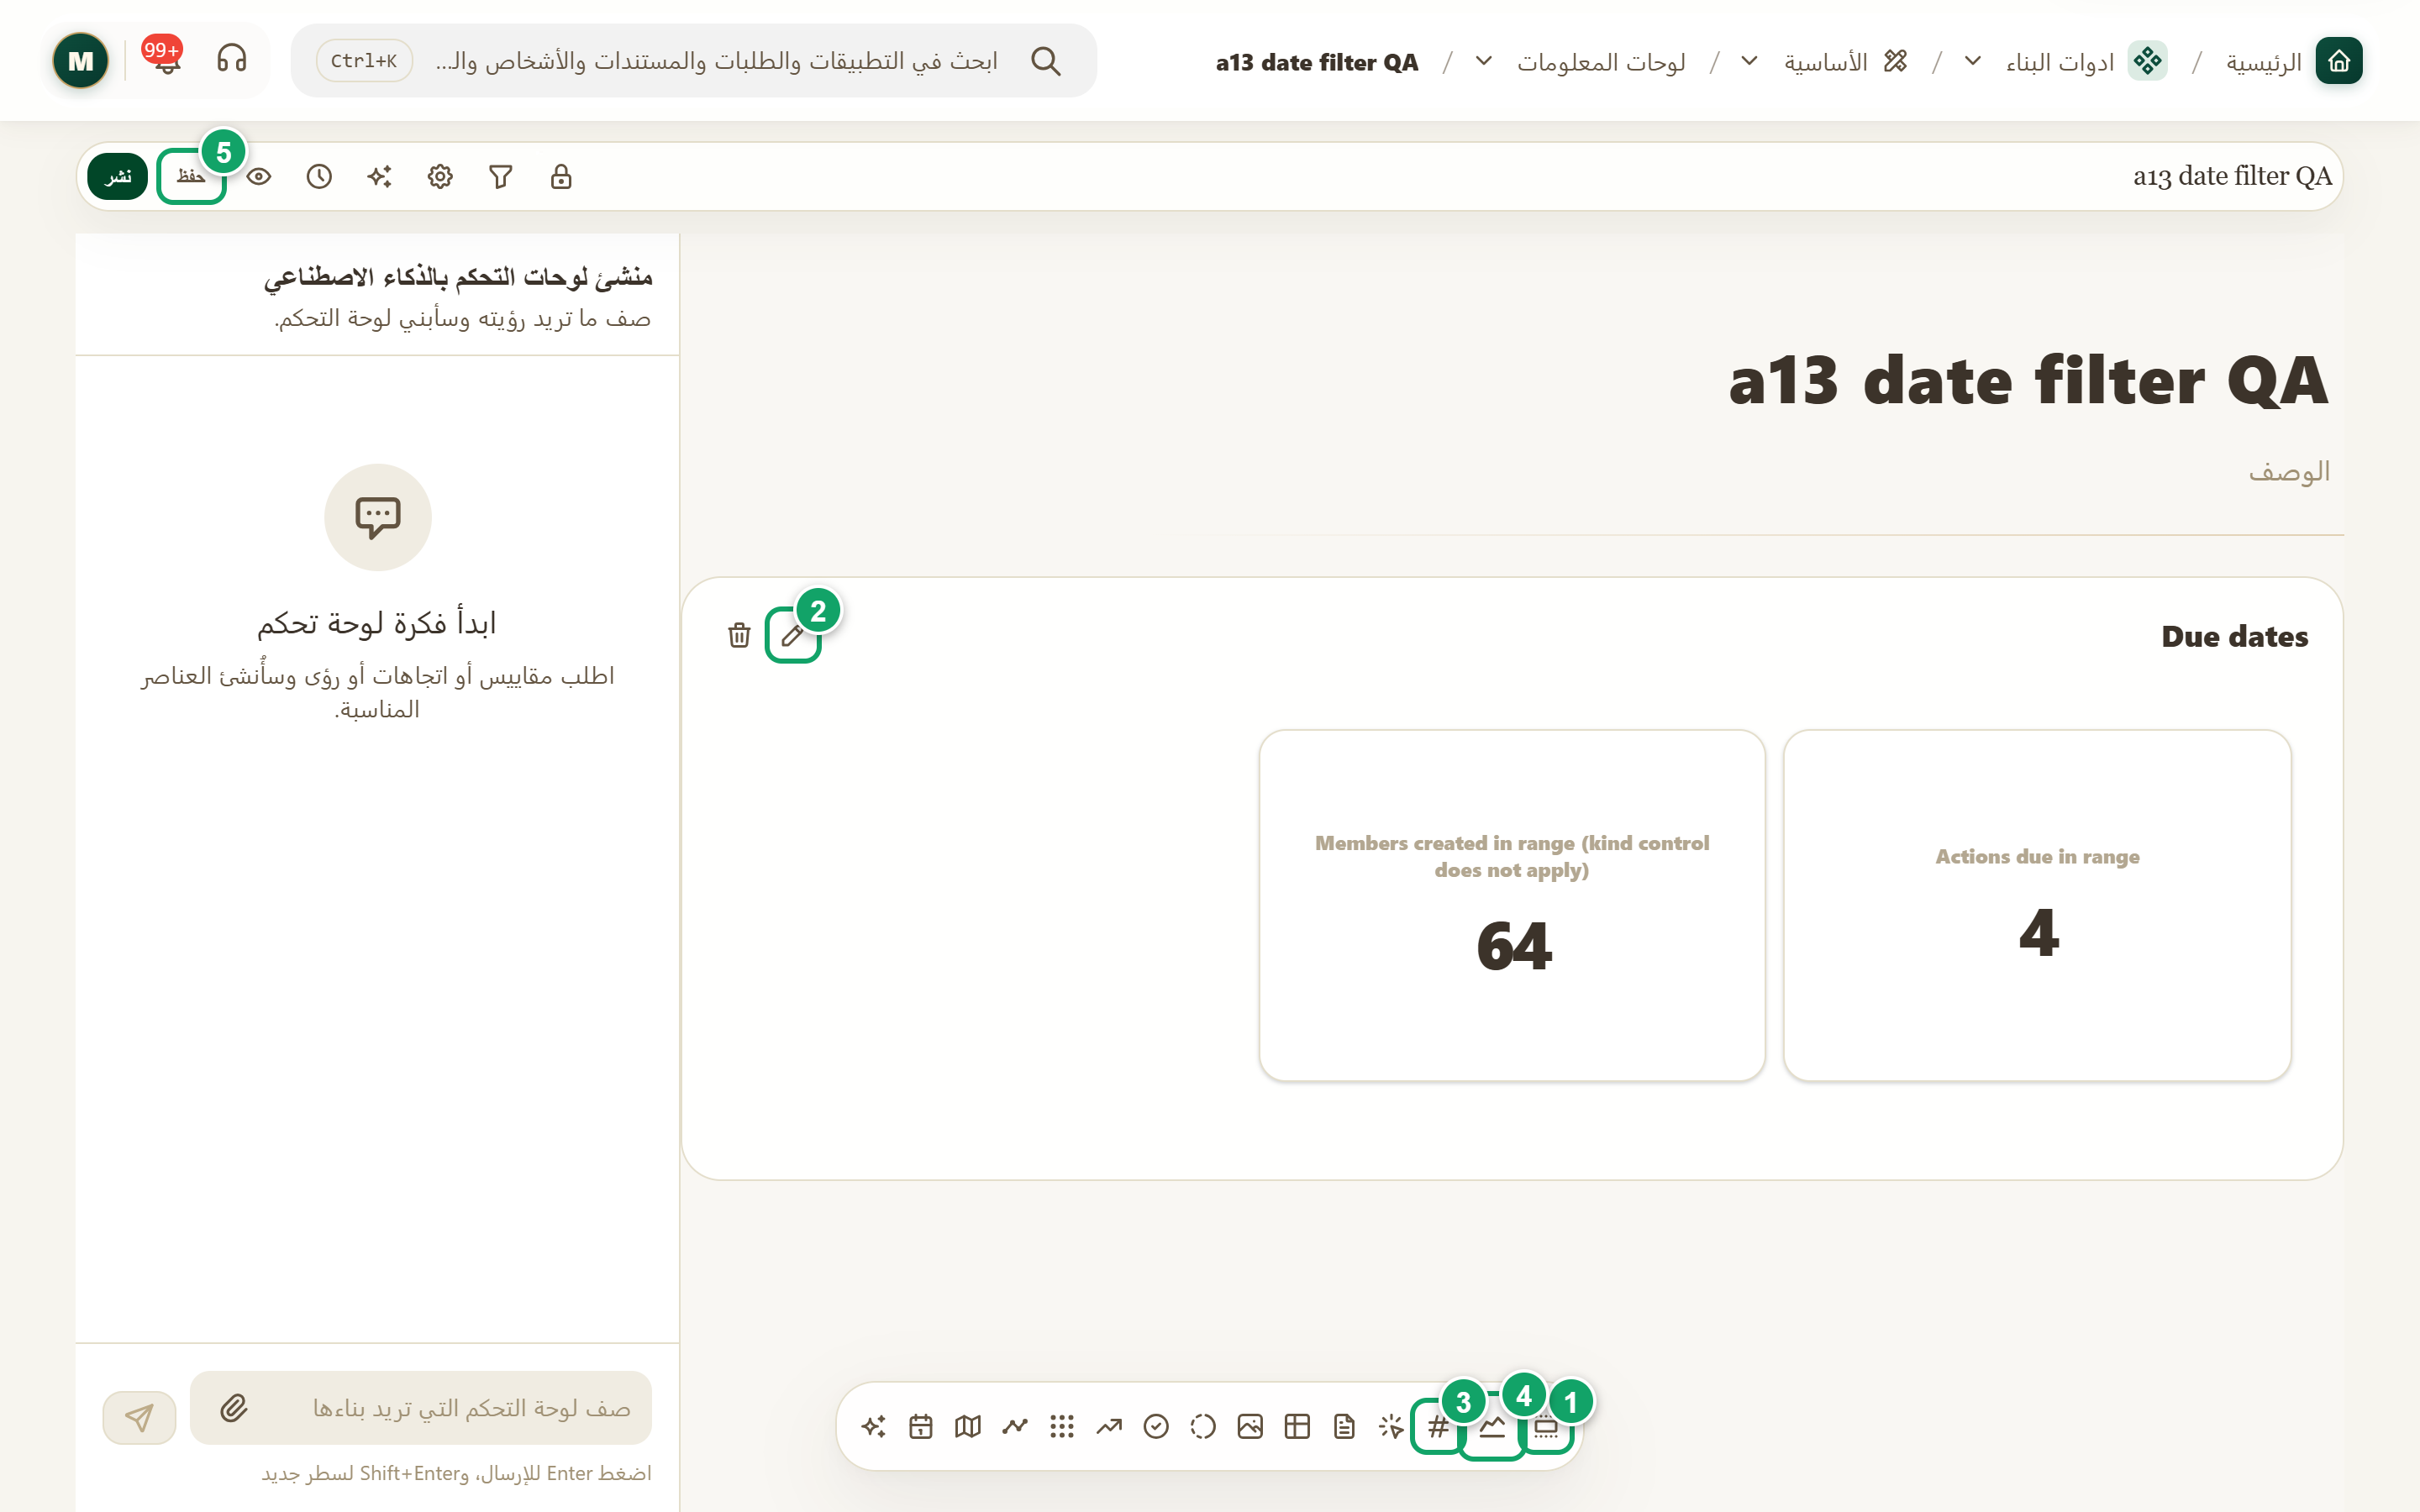
\includegraphics[width=0.95\linewidth,height=0.72\textheight,keepaspectratio]{figures/screens/ch06-dash-builder-ar.png}
\caption{منشئ اللوحة مع شريط الأدوات أسفل الصفحة}
\label{fig:builder-dashboards-builder-screen}
\shotnote{تعرض الصورة لوحة اختبار مفتوحة في المنشئ، فيها قسم واحد بعنصرين من نوع «رقم»، واللوحة الجانبية للذكاء الاصطناعي ظاهرة. ويجمع شريط الأدوات السفلي كل ما يضيف أقساماً وعناصر، بينما يجمع الرأس أزرار الضبط والحفظ. ① «إضافة قسم»: يضيف قسماً في آخر اللوحة. ② «تعديل»: زر القلم الذي يفتح عنوان القسم ووصفه. ③ «رقم»: يضيف عنصر رقم إلى آخر قسم. ④ زر الرسم البياني: يفتح قائمة «نوع الرسم البياني». ⑤ «حفظ»: يحفظ المسودة دون نشرها.}
\end{figure}

\begin{table}[H]
\centering
\caption{أزرار رأس المنشئ}
\label{tab:builder-dashboards-builder-header}
\begin{tabularx}{\linewidth}{R{3.6cm} Y}
\rcHeaderRow
\thh{الزر} & \thh{ما يفعله}\\
«إدارة الوصول» & يحدد من يستطيع فتح اللوحة، كما في صفحة «لوحات المعلومات».\\
«المرشحات» & يضيف المرشحات التي يغيّرها المشاهد، مثل نطاق التاريخ.\\
«الإعدادات» & يفتح إعدادات اللوحة: الاسم والوصف ومكان ظهورها في التنقل.\\
«منشئ لوحات التحكم بالذكاء الاصطناعي» & يُظهر اللوحة الجانبية التي تصف فيها ما تريد أو يخفيها، فيقترح الذكاء الاصطناعي العناصر.\\
«الإصدارات» و«معاينة» & يعرض الأول الإصدارات السابقة، ويعرض الثاني اللوحة كما يراها المشاهد.\\
«حفظ» و«نشر» & يحفظ الأول المسودة، ويحفظ الثاني ما في المنشئ ثم ينشره للمشاهدين.\\
\end{tabularx}
\end{table}

\begin{table}[H]
\centering
\caption{العمل على الأقسام والعناصر}
\label{tab:builder-dashboards-builder-grid}
\begin{tabularx}{\linewidth}{R{3.6cm} Y}
\rcHeaderRow
\thh{الإجراء} & \thh{كيف يتم}\\
إضافة قسم & اضغط «إضافة قسم» في شريط الأدوات أسفل الصفحة. ويُضاف القسم في آخر اللوحة.\\
تعديل القسم & اضغط زر القلم بجانب عنوانه، واكتب «عنوان القسم» و«الوصف»، ثم اضغط «حفظ». ويحذف زر سلة المهملات القسم.\\
إضافة عنصر & اضغط أيقونة نوع العنصر في شريط الأدوات، أو زر الرسم البياني لتختار من قائمة «نوع الرسم البياني». ويُضاف العنصر إلى آخر قسم، ويُضاف بجانب عنصر آخر إذا ضغطت علامة \en{+} عند حافته.\\
ترتيب العنصر & اسحبه داخل الشبكة أو غيّر حجمه من حافته. وتنقله قائمة «نقل العنصر» إلى الأعلى أو الأسفل أو الجانبين، أو إلى قسم آخر بأمر «نقل إلى القسم».\\
ضبط العنصر & اضغط العنصر لتفتح لوحة إعداداته، وفيها أيضاً «نسخ» لعمل نسخة منه و«حذف» لإزالته.\\
\end{tabularx}
\end{table}

\begin{rcwarn}[الرسم الجديد يبدأ ببيانات تجريبية]
يظهر الرسم البياني الجديد ببيانات تجريبية حتى تختار له مصدر بيانات حقيقياً. فلا تنشر اللوحة قبل أن تربط كل عنصر بمصدره، وإلا رأى المشاهدون أرقاماً لا تخص المؤسسة.
\end{rcwarn}

\begin{figure}[H]
\centering
\begin{tikzpicture}[node distance=0.5cm]
\node[stepBox] (a) {\RL{إضافة قسم}};
\node[stepBox,below=of a] (b) {\RL{إضافة عنصر إلى القسم}};
\node[stepBox,below=of b] (c) {\RL{ضبط العنصر من لوحة إعداداته}};
\node[stepBox,below=of c] (d) {\RL{ترتيب العناصر وتحديد أحجامها}};
\node[stepBox,below=of d] (e) {\RL{حفظ المسودة}};
\draw[flowsTo] (a) -- (b);
\draw[flowsTo] (b) -- (c);
\draw[flowsTo] (c) -- (d);
\draw[flowsTo] (d) -- (e);
\end{tikzpicture}
\rclegend
\caption{بناء محتوى اللوحة}
\label{fig:builder-dashboards-builder-flow}
\shotnote{يبدأ المخطط بالقسم لأن كل عنصر ينتمي إلى قسم، والعنصر الجديد يذهب إلى آخر قسم في اللوحة. ويأتي الترتيب بعد الضبط، لأن حجم العنصر المناسب لا يتضح إلا بعد أن يعرض بياناته الحقيقية. وينتهي المخطط بالحفظ، لأن ترتيب العناصر لا يُحفظ في المسودة إلا بضغط «حفظ» أو «نشر».}
\end{figure}

\subsection{خطوات العمل والتحقق}
\begin{enumerate}
\item افتح اللوحة في المنشئ، واضغط «إضافة قسم»، ثم اضغط زر القلم واكتب «عنوان القسم» واضغط «حفظ».
\item اضغط أيقونة «رقم» في شريط الأدوات، ثم زر الرسم البياني واختر «دائري» من «نوع الرسم البياني».
\item اضغط كل عنصر واضبط مصدر بياناته كما في صفحة «إعدادات العنصر ومصادر بياناته».
\item اسحب العناصر وغيّر أحجامها حتى يصبح القسم مقروءاً، ثم اضغط «حفظ».
\end{enumerate}

\textbf{تحقق ومعالجة المشكلة:} يجب أن تبقى الأقسام والعناصر في أماكنها بعد إعادة فتح المنشئ. فإذا اختفى عنصر أضفته، فابحث عنه في آخر قسم من اللوحة، ثم انقله بأمر «نقل إلى القسم». وإذا عرض رسم أرقاماً غريبة، فمصدره ما زال البيانات التجريبية.

\clearpage
\section{إعدادات العنصر ومصادر بياناته}
\label{sec:builder-feature-dashboards-widget-settings}

عندما تضغط عنصراً في المنشئ تُفتح لوحة إعداداته، وفيها ثلاثة تبويبات: «عام» للعنوان والحجم، و«البيانات» لمصدر الأرقام وطريقة حسابها، و«النمط» للألوان والشكل. ويحدد مصدر البيانات من أين يأخذ العنصر أرقامه، ويحدد «مستوى الوصول» هل يرى كل مشاهد ما تسمح به صلاحياته فقط.

\textbf{المسار ومن يستخدمه:} منشئ اللوحة ← اضغط العنصر ← لوحة الإعدادات. يستخدمها من يبني اللوحة، ويُفتح تبويب «البيانات» أولاً.

\begin{rcnote}[مثال: شركة الأفق]
يختار مسؤول النظام لعنصر الطلبات المنتظرة المصدر «كيان» ونوع السجلات «طلبات الزيارة»، ونوع القيمة «عدد»، ثم يضيف مرشحاً يقصر العدّ على الطلبات التي تنتظر المراجعة. ويختار «حسب صلاحيات المستخدم» فترى سارة الخطيب طلبات فروعها فقط.
\end{rcnote}

\begin{figure}[H]
\centering
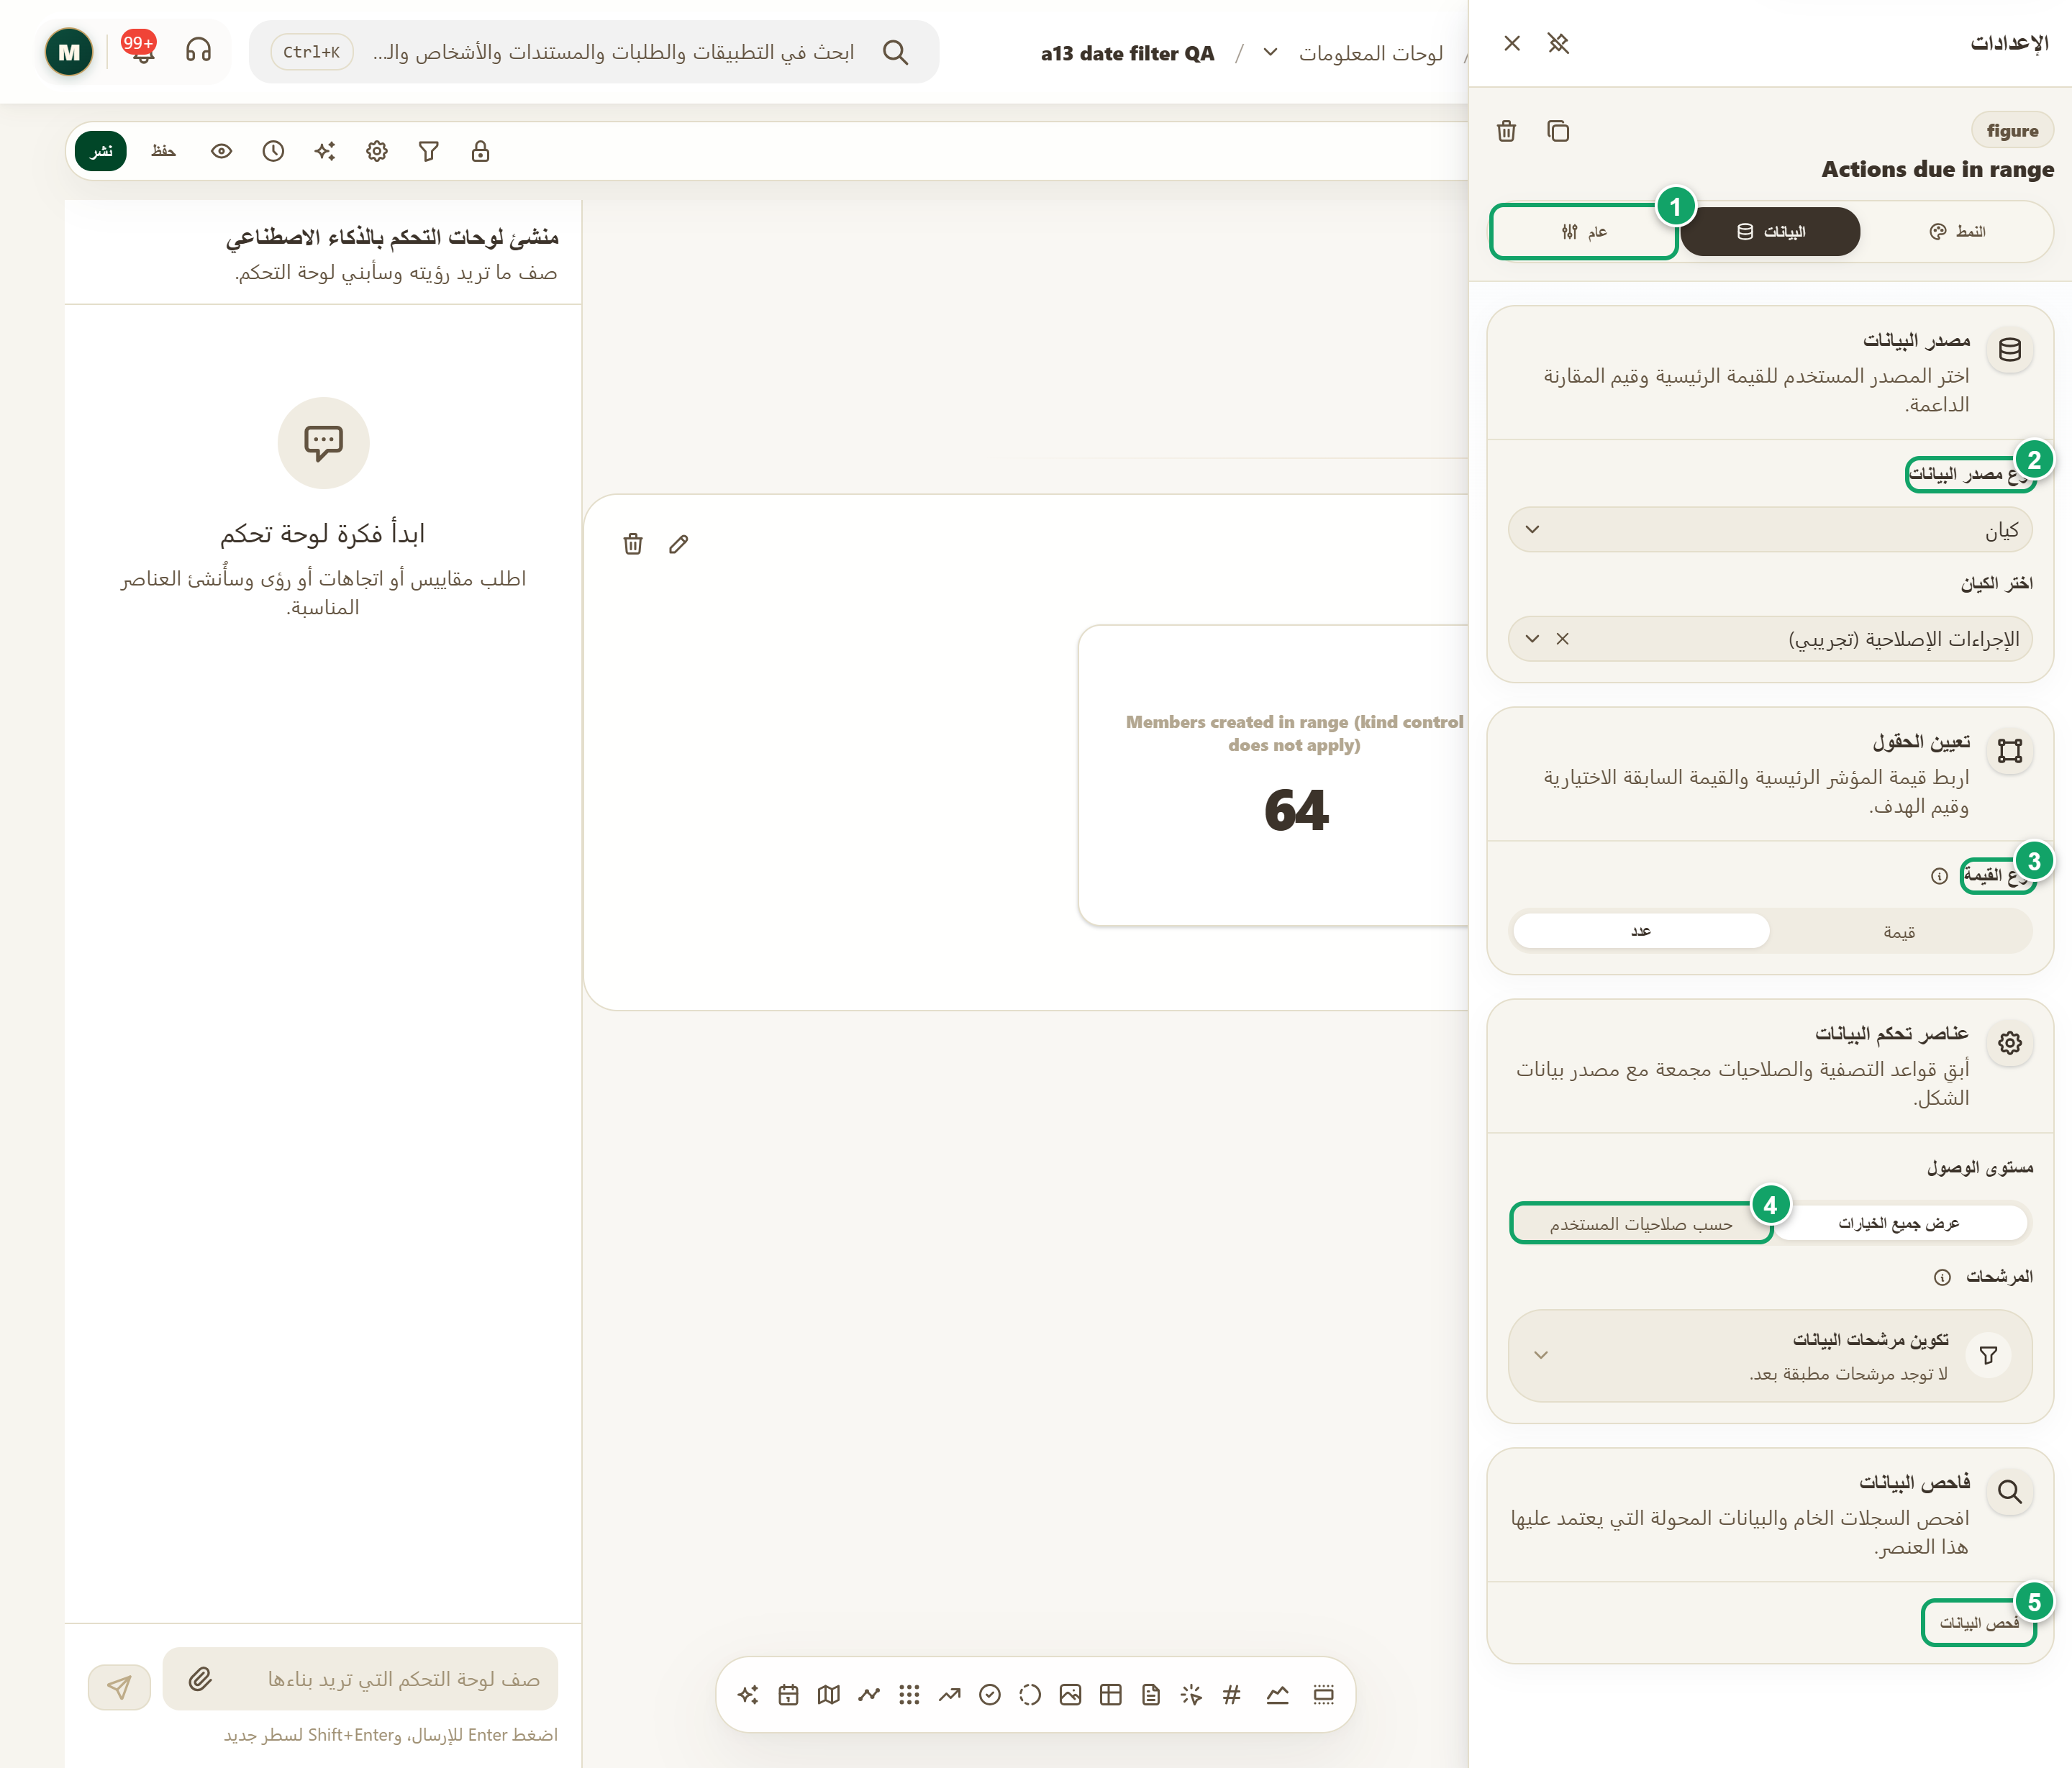
\includegraphics[width=0.95\linewidth,height=0.72\textheight,keepaspectratio]{figures/screens/ch06-dash-widget-settings-ar.png}
\caption{لوحة إعدادات عنصر «رقم» على تبويب «البيانات»}
\label{fig:builder-dashboards-widget-settings-screen}
\shotnote{تعرض الصورة لوحة الإعدادات بعد الضغط على عنصر «رقم» في لوحة اختبار، وقد فُتح تبويب «البيانات» تلقائياً. وفي هذا النوع يسمى قسم الصلاحيات والمرشحات «عناصر تحكم البيانات»، ويظهر فيه «مستوى الوصول» الذي يحدد ما يراه كل مشاهد. ① «عام»: العنوان والعرض والارتفاع. ② «نوع مصدر البيانات»: من أين يأخذ العنصر أرقامه. ③ «نوع القيمة»: «عدد» أو «قيمة». ④ «حسب صلاحيات المستخدم»: يحسب الرقم بصلاحيات من يفتح اللوحة. ⑤ «فحص البيانات»: يعرض السجلات التي قرأها العنصر.}
\end{figure}

\begin{table}[H]
\centering
\caption{مصادر البيانات في «نوع مصدر البيانات»}
\label{tab:builder-dashboards-widget-settings-sources}
\begin{tabularx}{\linewidth}{R{3.6cm} Y}
\rcHeaderRow
\thh{المصدر} & \thh{متى تستخدمه}\\
«كيان» & المصدر المعتاد: تختار نوع السجلات من «اختر الكيان»، ثم الحقول التي يعرضها العنصر أو يعدّها.\\
«إجراء تشغيلي» & يستدعي العنصر مشغّل ويب هوك في مسار إجراء تشغيلي ويعرض ما يعيده، ويجرّبه زر «اختبار SOP».\\
«خطة تكليف» & يعرض أرقام خطة تكليف وجولاتها، مثل عدد المهام المُسندة والمنجزة والمتأخرة.\\
«الفحوص والنتائج» & يعرض فحوص الجودة في نموذج تختاره: درجات الطلبات، أو الفحوص، أو نتائج الذكاء الاصطناعي.\\
«بيانات يدوية» & تكتب البيانات بنفسك بصيغة \en{JSON}، وتناسب مثالاً ثابتاً أو رقماً لا يُحفظ في النظام.\\
«المراسلات الرسمية» & يظهر لمن يملك تطبيق المراسلات، ويعرض الرسائل أو الأعمال أو السجل أو الأداء في فترة تختارها.\\
\end{tabularx}
\end{table}

\begin{table}[H]
\centering
\caption{ما تضبطه في التبويبات الثلاثة}
\label{tab:builder-dashboards-widget-settings-tabs}
\begin{tabularx}{\linewidth}{R{3.6cm} Y}
\rcHeaderRow
\thh{التبويب} & \thh{الإعدادات}\\
«عام» & «العنوان» الظاهر فوق العنصر، و«العرض» و«الارتفاع» بعدد خانات الشبكة.\\
«البيانات» & المصدر، ثم الحقول، و«نوع القيمة»: «عدد» لعدّ السجلات أو «قيمة» لحقل رقمي مع «التجميع» كالمجموع أو المتوسط.\\
«خيارات متقدمة ومرشحات» & داخل «البيانات»، وتسمى «عناصر تحكم البيانات» في عنصر «رقم»: «مستوى الوصول» بخياري «عرض جميع الخيارات» و«حسب صلاحيات المستخدم»، والمرشحات التي تضيّق السجلات، وخيار إخفاء العنصر عمّن لا يملك صلاحية.\\
«فاحص البيانات» & داخل «البيانات» أيضاً: يعرض زر «فحص البيانات» السجلات التي قرأها العنصر والبيانات بعد تحويلها، فتعرف سبب رقم غير متوقع.\\
«النمط» & الألوان والتسميات والخطوط وطريقة العرض. وتختلف خياراته بحسب نوع العنصر.\\
\end{tabularx}
\end{table}

\begin{rcwarn}[«عرض جميع الخيارات» يتجاوز صلاحيات المشاهد]
إذا اخترت «عرض جميع الخيارات» فسيرى كل من يفتح اللوحة أرقام جميع السجلات، حتى التي لا يستطيع فتحها. فاختر «حسب صلاحيات المستخدم» ما لم تكن الأرقام الكاملة مقصودة لكل من يصل إلى اللوحة.
\end{rcwarn}

\begin{figure}[H]
\centering
\begin{tikzpicture}[node distance=0.5cm]
\node[stepBox] (a) {\RL{اختيار نوع مصدر البيانات}};
\node[stepBox,below=of a] (b) {\RL{اختيار الكيان والحقول}};
\node[stepBox,below=of b] (c) {\RL{نوع القيمة والتجميع}};
\node[stepBox,below=of c] (d) {\RL{مستوى الوصول والمرشحات}};
\node[stepBox,below=of d] (e) {\RL{فاحص البيانات}};
\draw[flowsTo] (a) -- (b);
\draw[flowsTo] (b) -- (c);
\draw[flowsTo] (c) -- (d);
\draw[flowsTo] (d) -- (e);
\end{tikzpicture}
\rclegend
\caption{ضبط بيانات عنصر}
\label{fig:builder-dashboards-widget-settings-flow}
\shotnote{يتبع المخطط ترتيب تبويب «البيانات»: فالحقول المتاحة تعتمد على المصدر والكيان، والتجميع يعتمد على الحقل. ويأتي «فاحص البيانات» أخيراً لأنه يكشف أثر المرشحات ومستوى الوصول على الرقم قبل أن يراه أحد.}
\end{figure}

\subsection{خطوات العمل والتحقق}
\begin{enumerate}
\item اضغط العنصر في المنشئ، واكتب «العنوان» في تبويب «عام»، ثم اضبط «العرض» و«الارتفاع».
\item افتح «البيانات»، واختر «كيان» في «نوع مصدر البيانات»، ثم اختر نوع السجلات من «اختر الكيان».
\item اختر «عدد» أو «قيمة» في «نوع القيمة»، وحدد الحقل و«التجميع» عند الحاجة.
\item افتح «خيارات متقدمة ومرشحات»، واختر «حسب صلاحيات المستخدم»، وأضف المرشحات التي تقصر السجلات على ما تريد.
\item اضغط «فحص البيانات» وقارن السجلات المعروضة بما تعرفه، ثم اضبط الألوان في «النمط».
\end{enumerate}

\textbf{تحقق ومعالجة المشكلة:} يجب أن يطابق الرقم عدد السجلات التي تعرفها. فإذا ظهر «لا توجد بيانات»، فراجع المرشحات في «خيارات متقدمة ومرشحات». وإذا رأى مشاهد رسالة بأنه لا يملك صلاحية عرض البيانات، فهذا متوقع مع «حسب صلاحيات المستخدم»؛ فامنحه صلاحية قراءة النوع أو أخفِ العنصر عنه.

\clearpage
\section{أنواع العناصر}
\label{sec:builder-feature-dashboards-widgets}

يحدد نوع العنصر شكل عرض البيانات: رقم واحد، أو جدول، أو رسم بياني، أو تقويم، أو غير ذلك. ويضم شريط الأدوات في المنشئ ثلاثة عشر نوعاً، ويفتح زر الرسم البياني قائمة بواحد وثلاثين نوعاً من الرسوم. واختر النوع الذي يجيب عن سؤال المشاهد بأبسط شكل.

\textbf{المسار ومن يستخدمه:} منشئ اللوحة ← شريط الأدوات أسفل الصفحة. يستخدمه من يبني اللوحة، ويظهر اسم كل نوع عند تمرير المؤشر فوق أيقونته.

\begin{rcnote}[مثال: شركة الأفق]
يستخدم مسؤول النظام في لوحة «متابعة الزيارات» عنصر «رقم» للطلبات المنتظرة، ورسماً «دائري» للطلبات حسب الحالة، ورسم «أعمدة» للزيارات حسب الفرع، وعنصر «تقويم» لمواعيد الزيارات في فرع حلب وغيره.
\end{rcnote}

\begin{figure}[H]
\centering
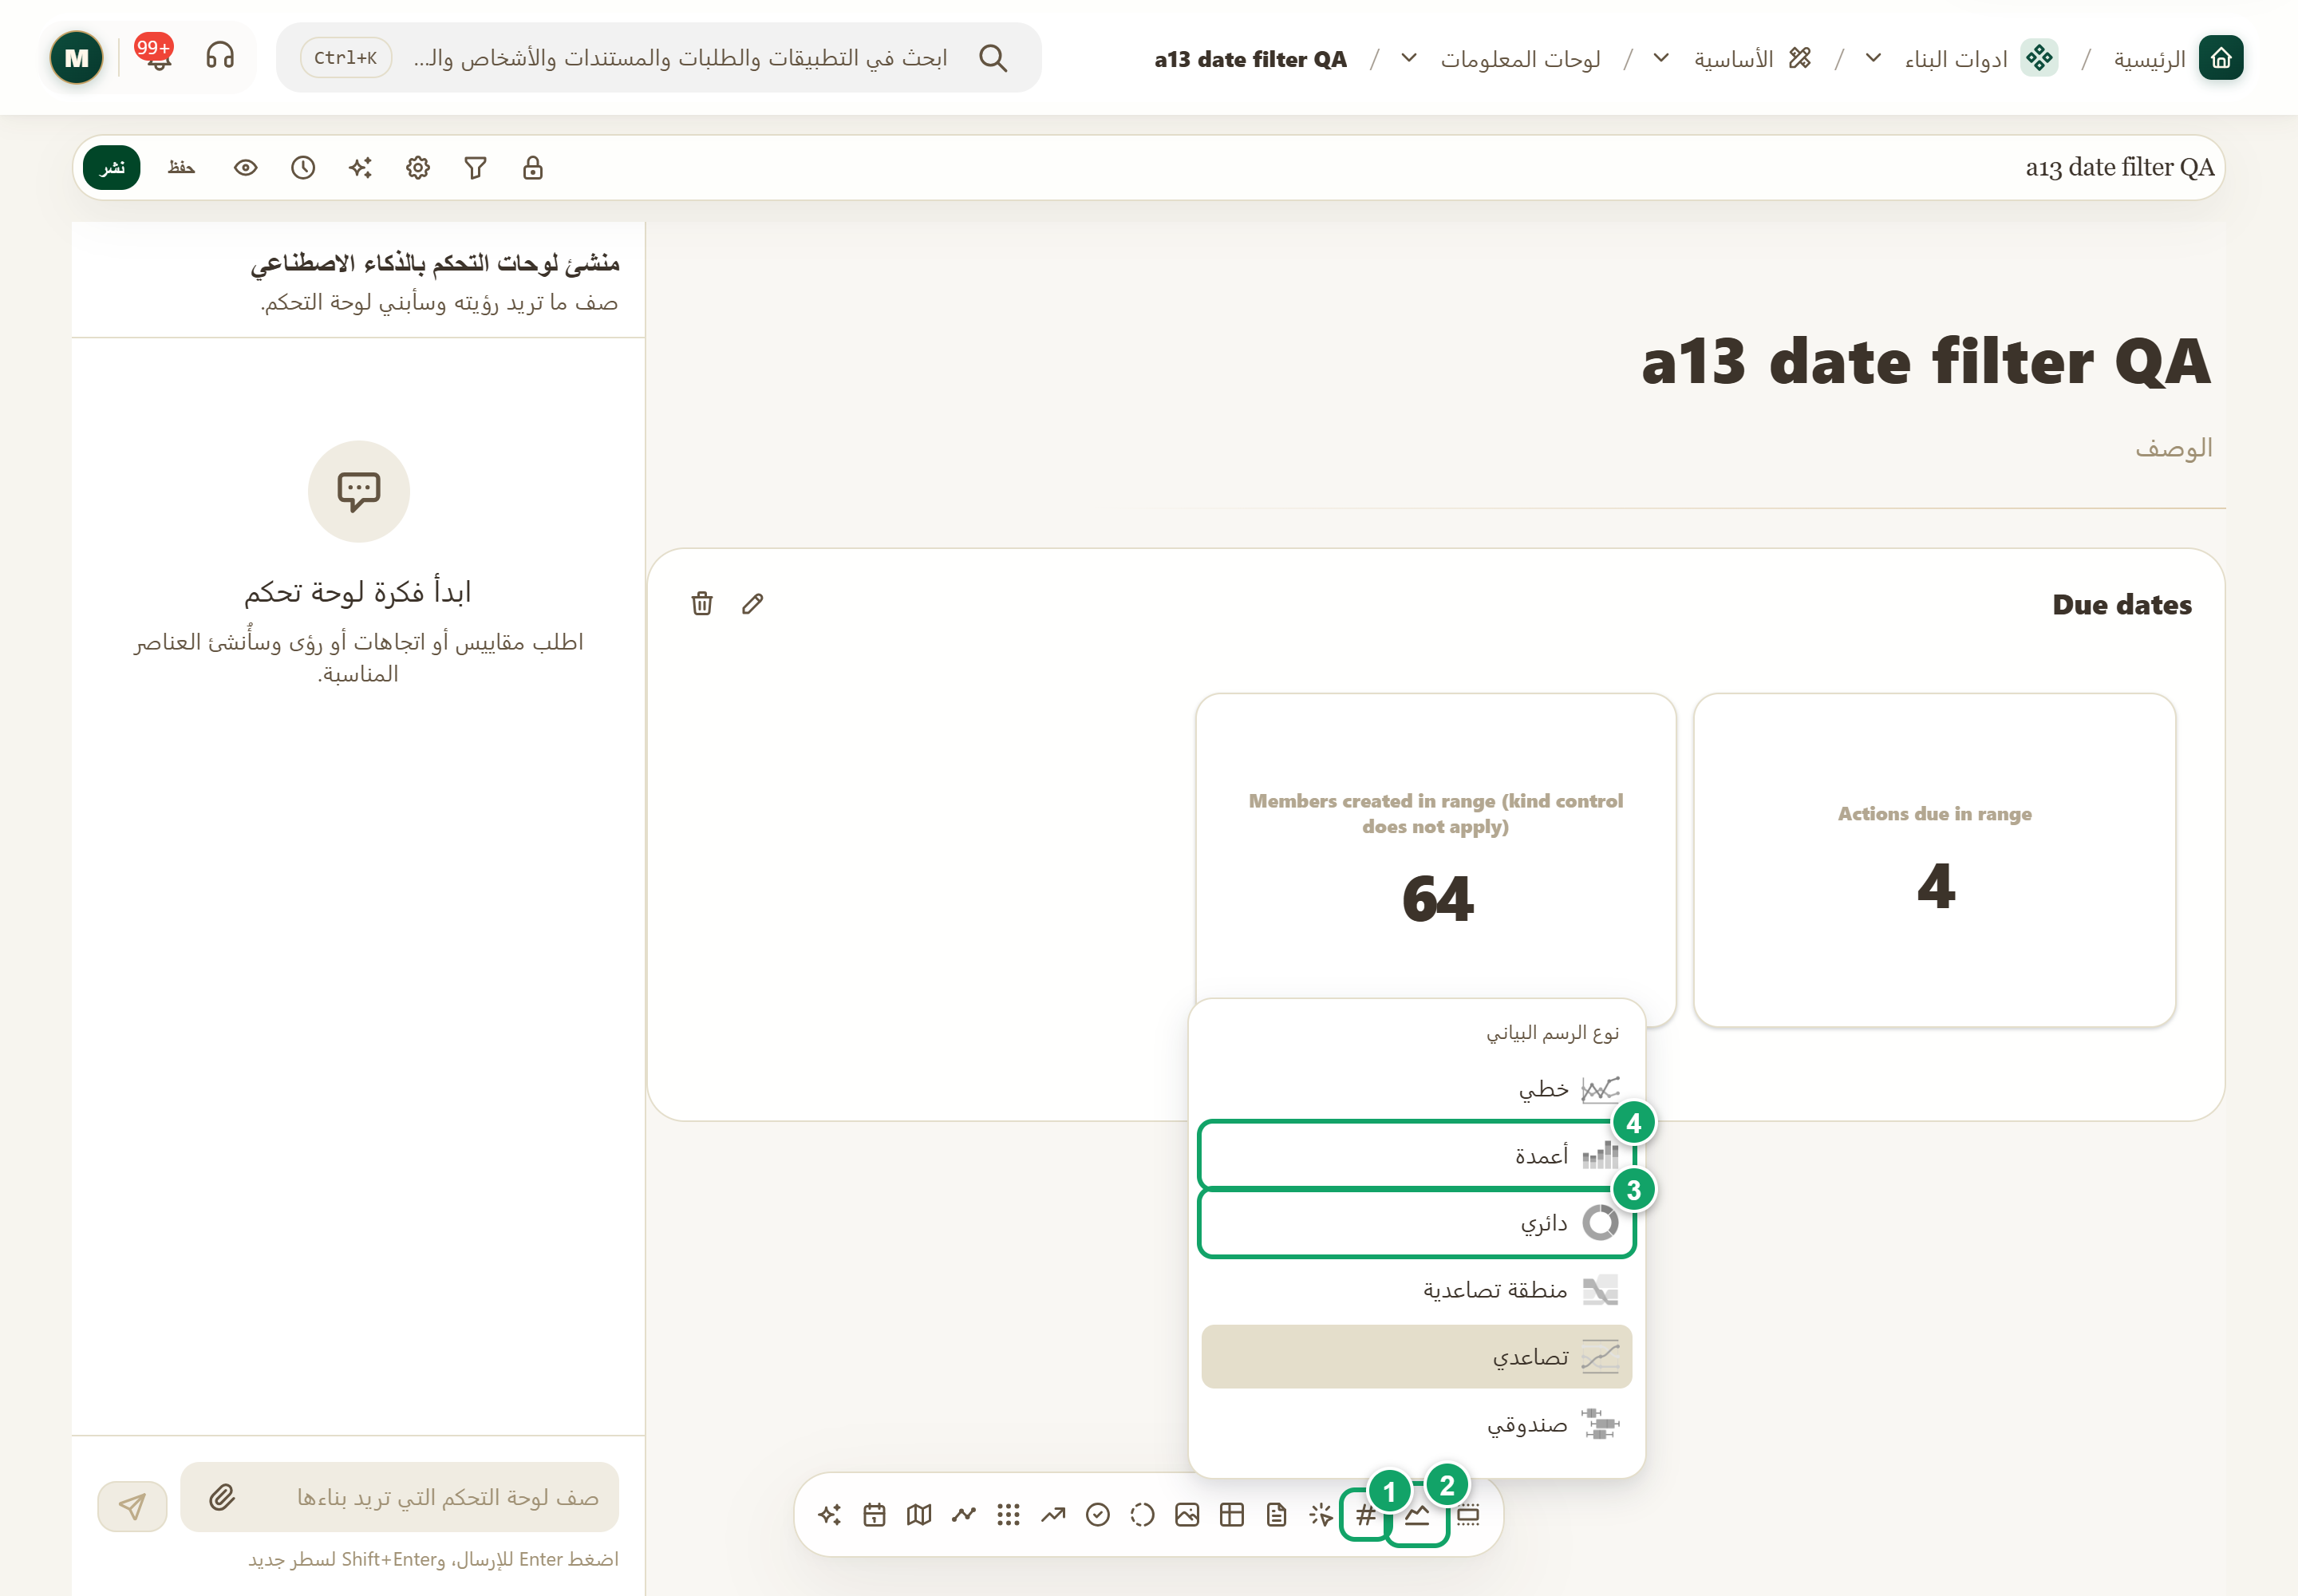
\includegraphics[width=0.95\linewidth,height=0.72\textheight,keepaspectratio]{figures/screens/ch06-dash-chart-types-ar.png}
\caption{قائمة «نوع الرسم البياني» فوق شريط الأدوات}
\label{fig:builder-dashboards-widgets-screen}
\shotnote{تعرض الصورة القائمة التي تفتح من زر الرسم البياني، وتظهر منها أوائل الرسوم، وتُعرض بقيتها بالتمرير داخل القائمة. أما الأنواع غير البيانية فلكل منها أيقونة مستقلة في شريط الأدوات يظهر اسمها عند تمرير المؤشر. ① «رقم»: أيقونة عنصر القيمة الواحدة. ② زر الرسم البياني: يفتح القائمة. ③ «دائري»: للأجزاء من الكل، مثل الطلبات حسب الحالة. ④ «أعمدة»: للمقارنة بين فئات، مثل الزيارات حسب الفرع.}
\end{figure}

\begin{table}[H]
\centering
\caption{أنواع العناصر في شريط الأدوات}
\label{tab:builder-dashboards-widgets-types}
\begin{tabularx}{\linewidth}{R{3.6cm} Y}
\rcHeaderRow
\thh{المجموعة} & \thh{الأنواع ومتى تستخدم كلاً منها}\\
الأساسية & «رقم» لقيمة واحدة مع قيمة سابقة أو هدف عند الحاجة، و«جدول» لعرض السجلات في أعمدة تختارها، و«نص» لنص ثابت أو قيمة من حقل، و«صورة» من رابط أو حقل، و«زر» ينقل إلى صفحة أو نموذج أو رابط.\\
الحالة والتقدم & «تقدم» لنسبة قيمة إلى حد أعلى، و«حالة» لشارة يتغير لونها بحسب قيمة حقل، و«مؤشر أداء» لقيمة رئيسية مع مقارنة وهدف وألوان حدود.\\
عناصر خاصة & «خريطة حرارية» لجدول صفوف وأعمدة تُلوَّن خلاياه بحسب القيمة، و«الجدول الزمني» لأحداث مرتبة بالتاريخ، و«خريطة» لمواقع السجلات، و«تقويم» لمواعيدها.\\
تحليل بالذكاء الاصطناعي & «تحليل الذكاء الاصطناعي» يقرأ صفوفاً من مصدر أو أكثر ويكتب تحليلاً بحسب «توجيه التحليل»، ثم يجيب عن أسئلة المتابعة.\\
\end{tabularx}
\end{table}

\begin{table}[H]
\centering
\caption{الرسوم البيانية في «نوع الرسم البياني»}
\label{tab:builder-dashboards-widgets-charts}
\begin{tabularx}{\linewidth}{R{3.6cm} Y}
\rcHeaderRow
\thh{الغرض} & \thh{الرسوم المناسبة}\\
المقارنة بين فئات & «أعمدة»، و«أعمدة قطبية»، و«أعمدة شعاعية»، و«رادار».\\
التغير مع الزمن & «خطي»، و«تدفق»، و«تصاعدي»، و«تقويم» يلوّن أيام السنة، و«نطاق زمني».\\
الأجزاء من الكل & «دائري»، و«وافل»، و«خريطة شجرية»، و«شعاعي متشعب»، و«دوائر متداخلة».\\
المراحل والتدفق & «قمع» لمراحل يتناقص عددها، و«سانكي» لانتقال الكميات بين المراحل.\\
التوزيع والعلاقة & «مبعثر»، و«صندوقي»، و«سرب نقاط»، و«خريطة حرارية»، و«إحداثيات متوازية».\\
الخرائط & «مناطق لونية» لتلوين المناطق بحسب القيمة، و«خريطة جغرافية» لرسم المناطق.\\
\end{tabularx}
\end{table}

وتبقى في القائمة رسوم متخصصة أخرى، مثل «وتري» و«شبكة» و«شجرة» و«جليدي». وتضبط مظهر أي رسم من «خيارات الرسم البياني» في تبويب «النمط»، وتعيدها إلى أصلها بزر «إعادة التعيين إلى الافتراضي».

\begin{figure}[H]
\centering
\begin{tikzpicture}[node distance=0.5cm]
\node[stepBox] (a) {\RL{ما السؤال الذي يجيب عنه العنصر؟}};
\node[stepBox,below=of a] (b) {\RL{رقم واحد أم قائمة أم رسم؟}};
\node[stepBox,below=of b] (c) {\RL{اختيار النوع وإضافته}};
\node[stepBox,below=of c] (d) {\RL{ربطه بمصدر البيانات}};
\draw[flowsTo] (a) -- (b);
\draw[flowsTo] (b) -- (c);
\draw[flowsTo] (c) -- (d);
\end{tikzpicture}
\rclegend
\caption{اختيار نوع العنصر}
\label{fig:builder-dashboards-widgets-flow}
\shotnote{يبدأ المخطط بسؤال المشاهد لا بشكل الرسم، لأن النوع المناسب يتبع ما يريد المشاهد معرفته. فالعدد الحالي يكفيه «رقم»، والمقارنة بين الفروع تحتاج إلى «أعمدة»، والمواعيد تُفهم أسرع في «تقويم».}
\end{figure}

\subsection{خطوات العمل والتحقق}
\begin{enumerate}
\item اكتب السؤال الذي يجيب عنه العنصر، مثل «كم طلباً ينتظر المراجعة؟».
\item اختر من الجدولين النوع الذي يجيب عنه، ومرّر المؤشر فوق أيقونات شريط الأدوات حتى تجد اسمه.
\item اضغط الأيقونة، أو زر الرسم البياني ثم اسم الرسم في «نوع الرسم البياني».
\item اضبط مصدر البيانات والحقول المطلوبة لهذا النوع، ثم راجع شكله في «معاينة».
\end{enumerate}

\textbf{تحقق ومعالجة المشكلة:} يجب أن يجيب العنصر عن سؤاله من نظرة واحدة. فإذا ازدحم الرسم بفئات كثيرة، فاستخدم «جدول» أو أضف مرشحاً يقلل الفئات. وإذا لم يعرض «تحليل الذكاء الاصطناعي» نتيجة، فاضغط «إنشاء النتيجة»، لأن المنشئ يوقف التحليل أثناء التعديل.

\clearpage
\section{إعدادات اللوحة}
\label{sec:builder-feature-dashboards-settings}

تحدد إعدادات اللوحة اسمها ووصفها ومكان ظهورها في تنقل التطبيقات. وقد تظهر فيها أيضاً إعدادات تتحكم في البيانات التي يراها المشاهد، عندما تكون ميزات التنقل حسب العمل مفعّلة في المؤسسة.

\textbf{المسار ومن يستخدمه:} منشئ اللوحة ← «الإعدادات» ← نافذة «إعدادات لوحة المعلومات». يستخدمها من يبني اللوحة، ثم يضغط «حفظ».

\begin{rcnote}[مثال: شركة الأفق]
يفعّل مسؤول النظام «إظهار في التنقل» للوحة «متابعة الزيارات»، ويختار «خدمات الفروع» في «التطبيق» وقسم الزيارات في «قسم التطبيق»، فتظهر اللوحة لسارة الخطيب داخل التطبيق الذي تعمل فيه.
\end{rcnote}

\begin{figure}[H]
\centering
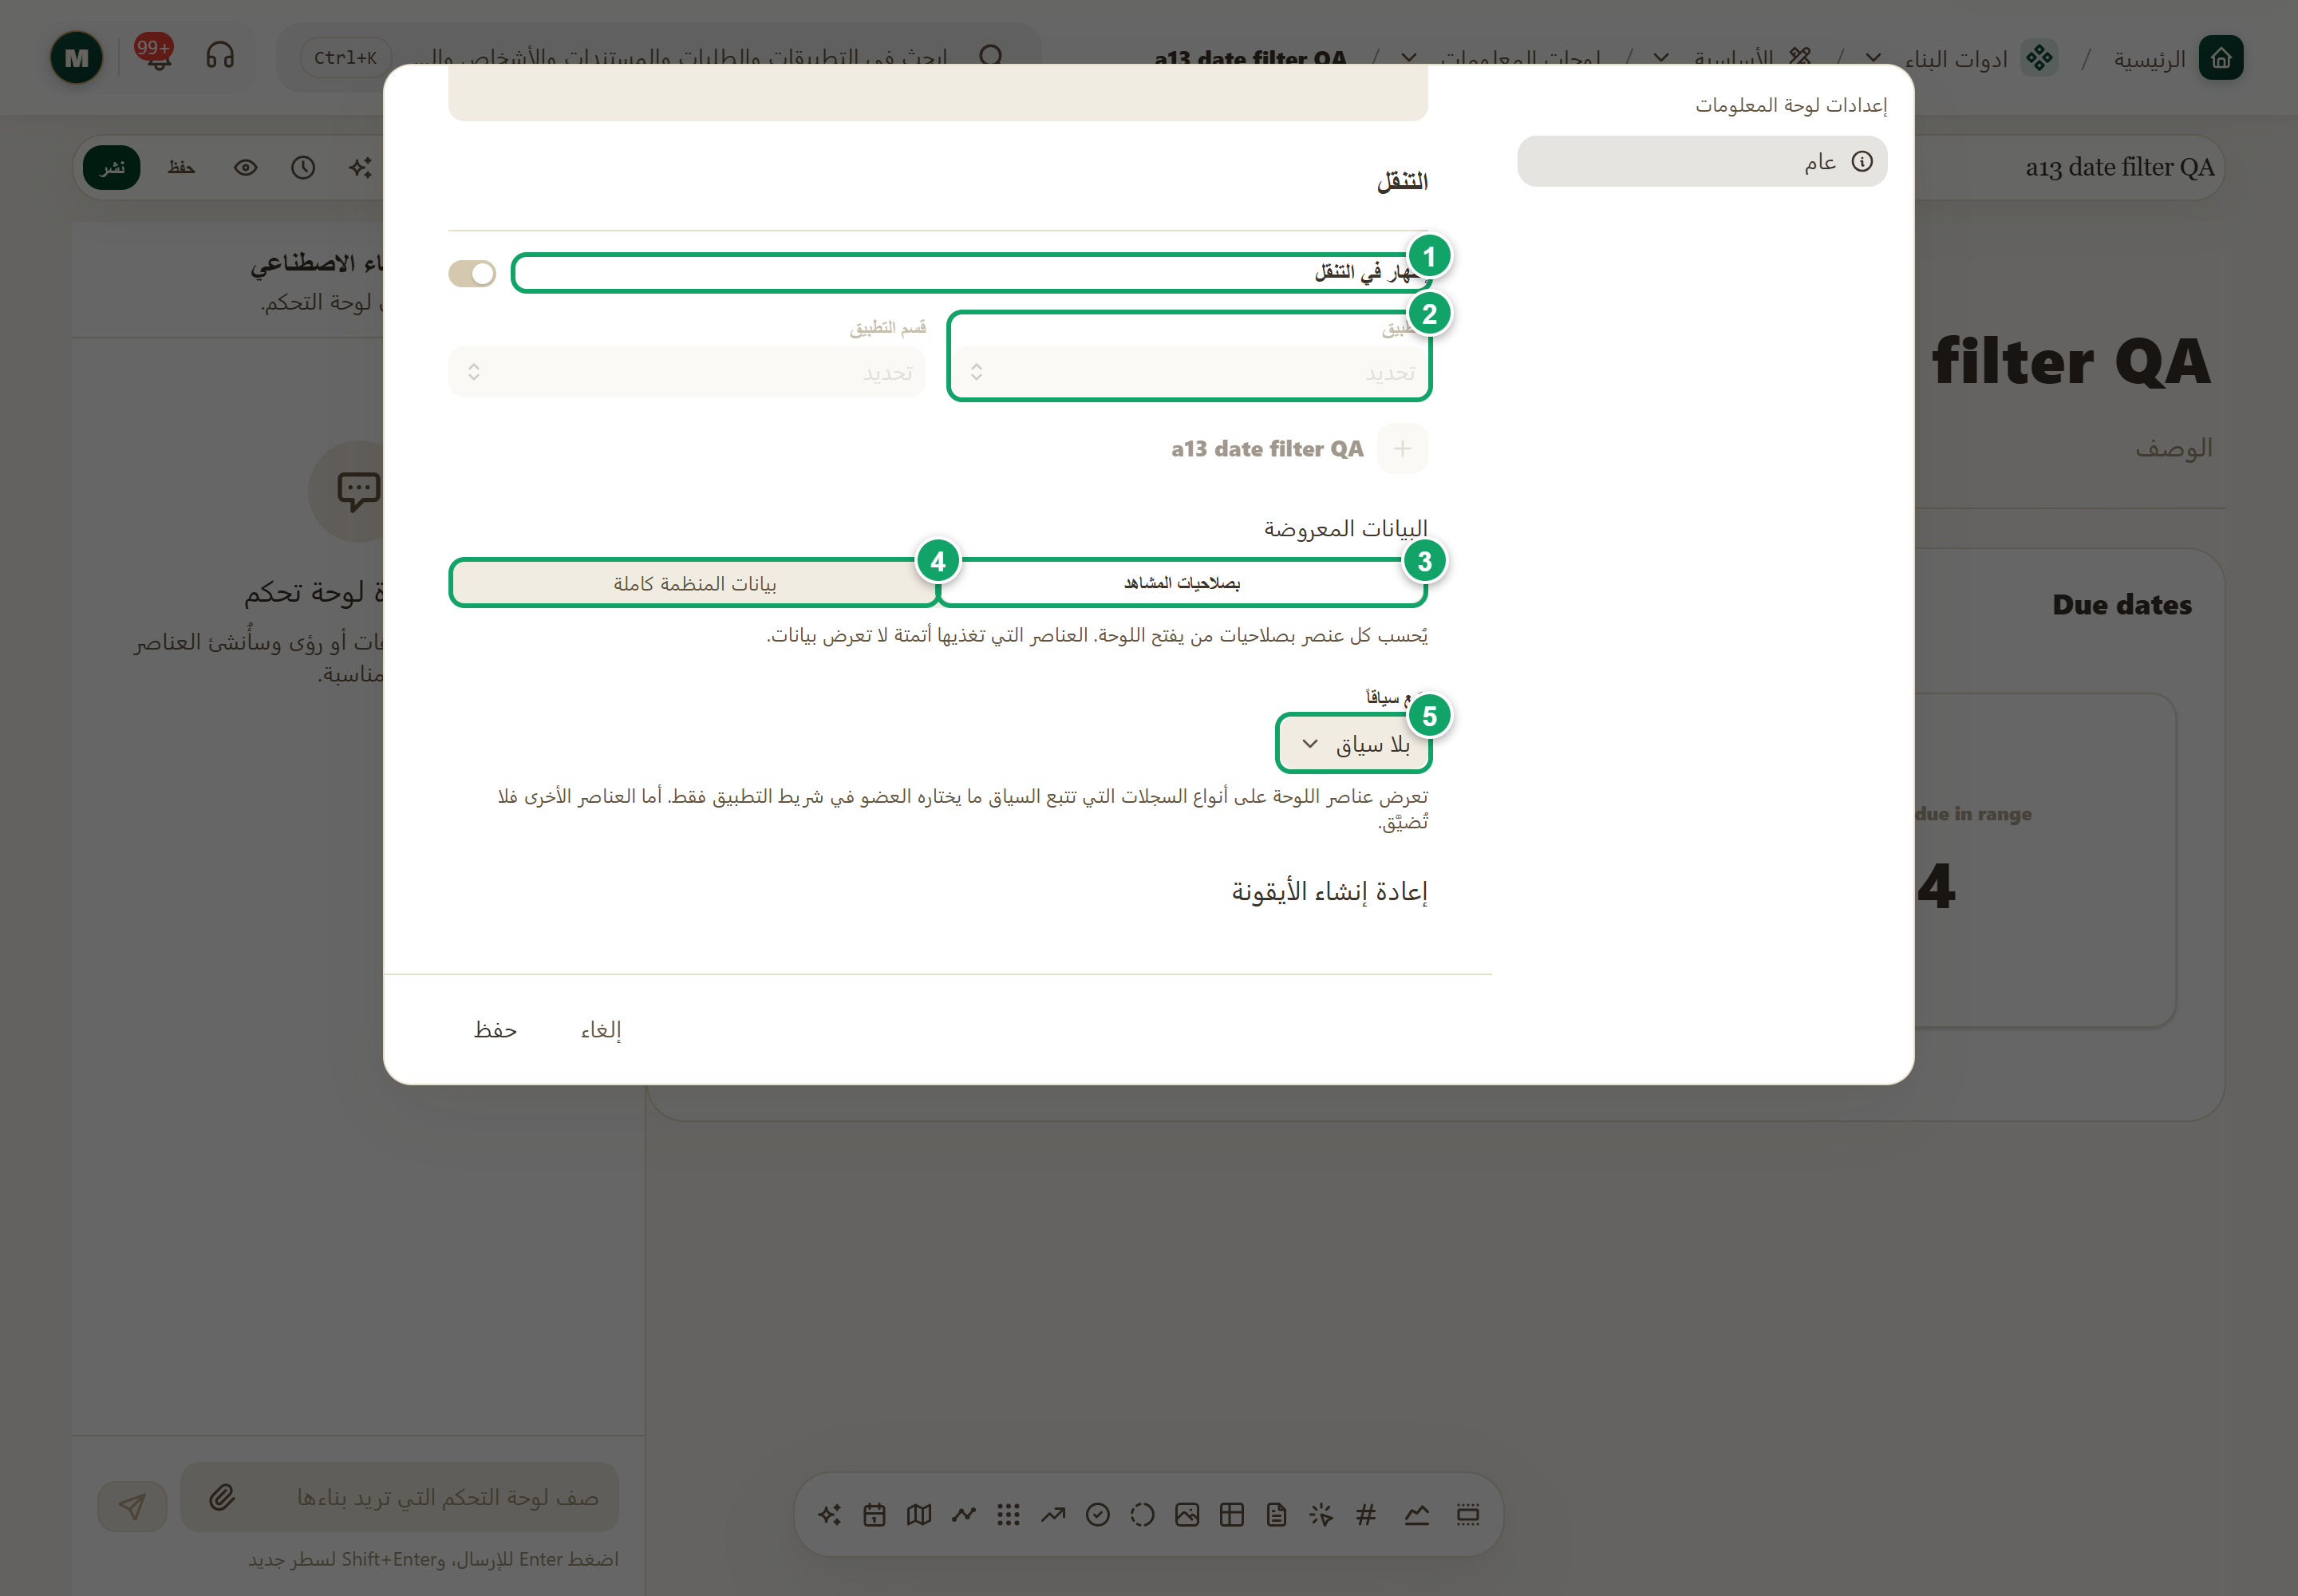
\includegraphics[width=0.95\linewidth,height=0.72\textheight,keepaspectratio]{figures/screens/ch06-dash-settings-ar.png}
\caption{نافذة «إعدادات لوحة المعلومات» بعد التمرير إلى قسم «التنقل»}
\label{fig:builder-dashboards-settings-screen}
\shotnote{تعرض الصورة نافذة إعدادات لوحة اختبار بعد التمرير إلى إعدادات الظهور والبيانات، والاسم والوصف أعلاها. ويظهر فيها «البيانات المعروضة» و«يتبع سياقاً» لأن هذه الميزات مفعّلة في مؤسسة الاختبار، وقد لا تظهر في مؤسستك. ① «إظهار في التنقل»: يضيف اللوحة إلى قائمة التطبيق. ② «التطبيق»: يتاح بعد التفعيل، ويليه «قسم التطبيق». ③ «بصلاحيات المشاهد»: الخيار الآمن الذي يحسب كل عنصر بصلاحيات من يفتح اللوحة. ④ «بيانات المنظمة كاملة»: يختاره مالك المؤسسة أو مسؤولها فقط. ⑤ «يتبع سياقاً»: يقصر العناصر على السياق المختار، و«بلا سياق» يتركها دون تضييق.}
\end{figure}

\begin{table}[H]
\centering
\caption{حقول «إعدادات لوحة المعلومات»}
\label{tab:builder-dashboards-settings-fields}
\begin{tabularx}{\linewidth}{R{3.6cm} Y}
\rcHeaderRow
\thh{الحقل} & \thh{المعنى}\\
«اسم لوحة المعلومات» و«الوصف» & الاسم الظاهر في القائمة والتنقل بكل لغة، ووصف قصير لما تتابعه اللوحة.\\
«إظهار في التنقل» & يضيف اللوحة عنصراً في قائمة التطبيق، مع أيقونة تختارها.\\
«التطبيق» و«قسم التطبيق» & التطبيق والقسم اللذان تظهر فيهما اللوحة.\\
«البيانات المعروضة» & «بصلاحيات المشاهد» فيُحسب كل عنصر بصلاحيات من يفتح اللوحة، أو «بيانات المنظمة كاملة» فيحتفظ كل عنصر بإعداد الوصول الخاص به. ولا يختار الخيار الثاني إلا مالك المؤسسة أو مسؤولها.\\
«يتبع سياقاً» & يقصر عناصر أنواع السجلات المرتبطة بسياق على ما يختاره العضو في شريط التطبيق، مثل فرع معين. والخيار «بلا سياق» يترك العناصر دون تضييق.\\
\end{tabularx}
\end{table}

\begin{rcwarn}[انتبه إلى «بيانات المنظمة كاملة»]
مع هذا الخيار يرى كل من يستطيع فتح اللوحة جميع السجلات في العناصر المضبوطة على «عرض جميع الخيارات»، ولو كانت صلاحياته أضيق. ولا تعرض العناصر التي تغذيها أتمتة أي بيانات مع «بصلاحيات المشاهد».
\end{rcwarn}

\begin{figure}[H]
\centering
\begin{tikzpicture}[node distance=0.5cm]
\node[stepBox] (a) {\RL{الاسم والوصف}};
\node[stepBox,below=of a] (b) {\RL{إظهار في التنقل}};
\node[stepBox,below=of b] (c) {\RL{التطبيق وقسم التطبيق}};
\node[stepBox,below=of c] (d) {\RL{البيانات المعروضة والسياق}};
\node[stepBox,below=of d] (e) {\RL{حفظ ثم نشر}};
\draw[flowsTo] (a) -- (b);
\draw[flowsTo] (b) -- (c);
\draw[flowsTo] (c) -- (d);
\draw[flowsTo] (d) -- (e);
\end{tikzpicture}
\rclegend
\caption{ضبط إعدادات اللوحة}
\label{fig:builder-dashboards-settings-flow}
\shotnote{يجمع المخطط قرارين: أين تظهر اللوحة، وأي بيانات يراها من يفتحها. ويُحسم مكان الظهور أولاً لأن السياق المقترح يعتمد على التطبيق والقسم، ثم يُحفظ كل ذلك وتُنشر اللوحة ليصل التغيير إلى المشاهدين.}
\end{figure}

\subsection{خطوات العمل والتحقق}
\begin{enumerate}
\item في المنشئ اضغط «الإعدادات»، وراجع «اسم لوحة المعلومات» و«الوصف».
\item فعّل «إظهار في التنقل»، واختر «التطبيق» ثم «قسم التطبيق» وأيقونة مناسبة.
\item إذا ظهر «البيانات المعروضة»، فاختر «بصلاحيات المشاهد» ما لم تحتج إلى غير ذلك.
\item إذا ظهر «يتبع سياقاً»، فاختر السياق الذي تتبعه اللوحة أو «بلا سياق»، ثم اضغط «حفظ» وانشر اللوحة.
\end{enumerate}

\textbf{تحقق ومعالجة المشكلة:} يجب أن تظهر اللوحة في القسم المختار من التطبيق. فإذا لم تظهر، فتأكد أن «إظهار في التنقل» مفعّل وأن اللوحة منشورة. وإذا رُفض اختيار «بيانات المنظمة كاملة»، فلا يختاره إلا مالك المؤسسة أو مسؤولها.

\clearpage
\section{مرشحات المشاهد ومحددات الكيانات}
\label{sec:builder-feature-dashboards-filters}

مرشحات المشاهد أدوات تظهر أعلى اللوحة، يغيّر بها المشاهد ما تعرضه العناصر دون أن يعدّل اللوحة. وتتيح ثلاثة أنواع: «نطاق التاريخ» لتحديد فترة، و«محدد» لاختيار سجل من نوع سجلات مثل فرع، و«اختر الحقل» لاختيار قيمة من قائمة خيارات. ولكل مرشح «النطاق» الذي يحدد العناصر التي يؤثر فيها.

\textbf{المسار ومن يستخدمه:} منشئ اللوحة ← «المرشحات». يضبطها من يبني اللوحة، ويستخدمها كل من يفتح اللوحة.

\begin{rcnote}[مثال: شركة الأفق]
يضيف مسؤول النظام إلى لوحة «متابعة الزيارات» مرشح «نطاق التاريخ» على تاريخ الزيارة، ومرشح «محدد» للفروع. فتختار سارة الخطيب فرع حلب والشهر الماضي، فتعرض كل العناصر زيارات ذلك الفرع في تلك الفترة.
\end{rcnote}

\begin{figure}[H]
\centering
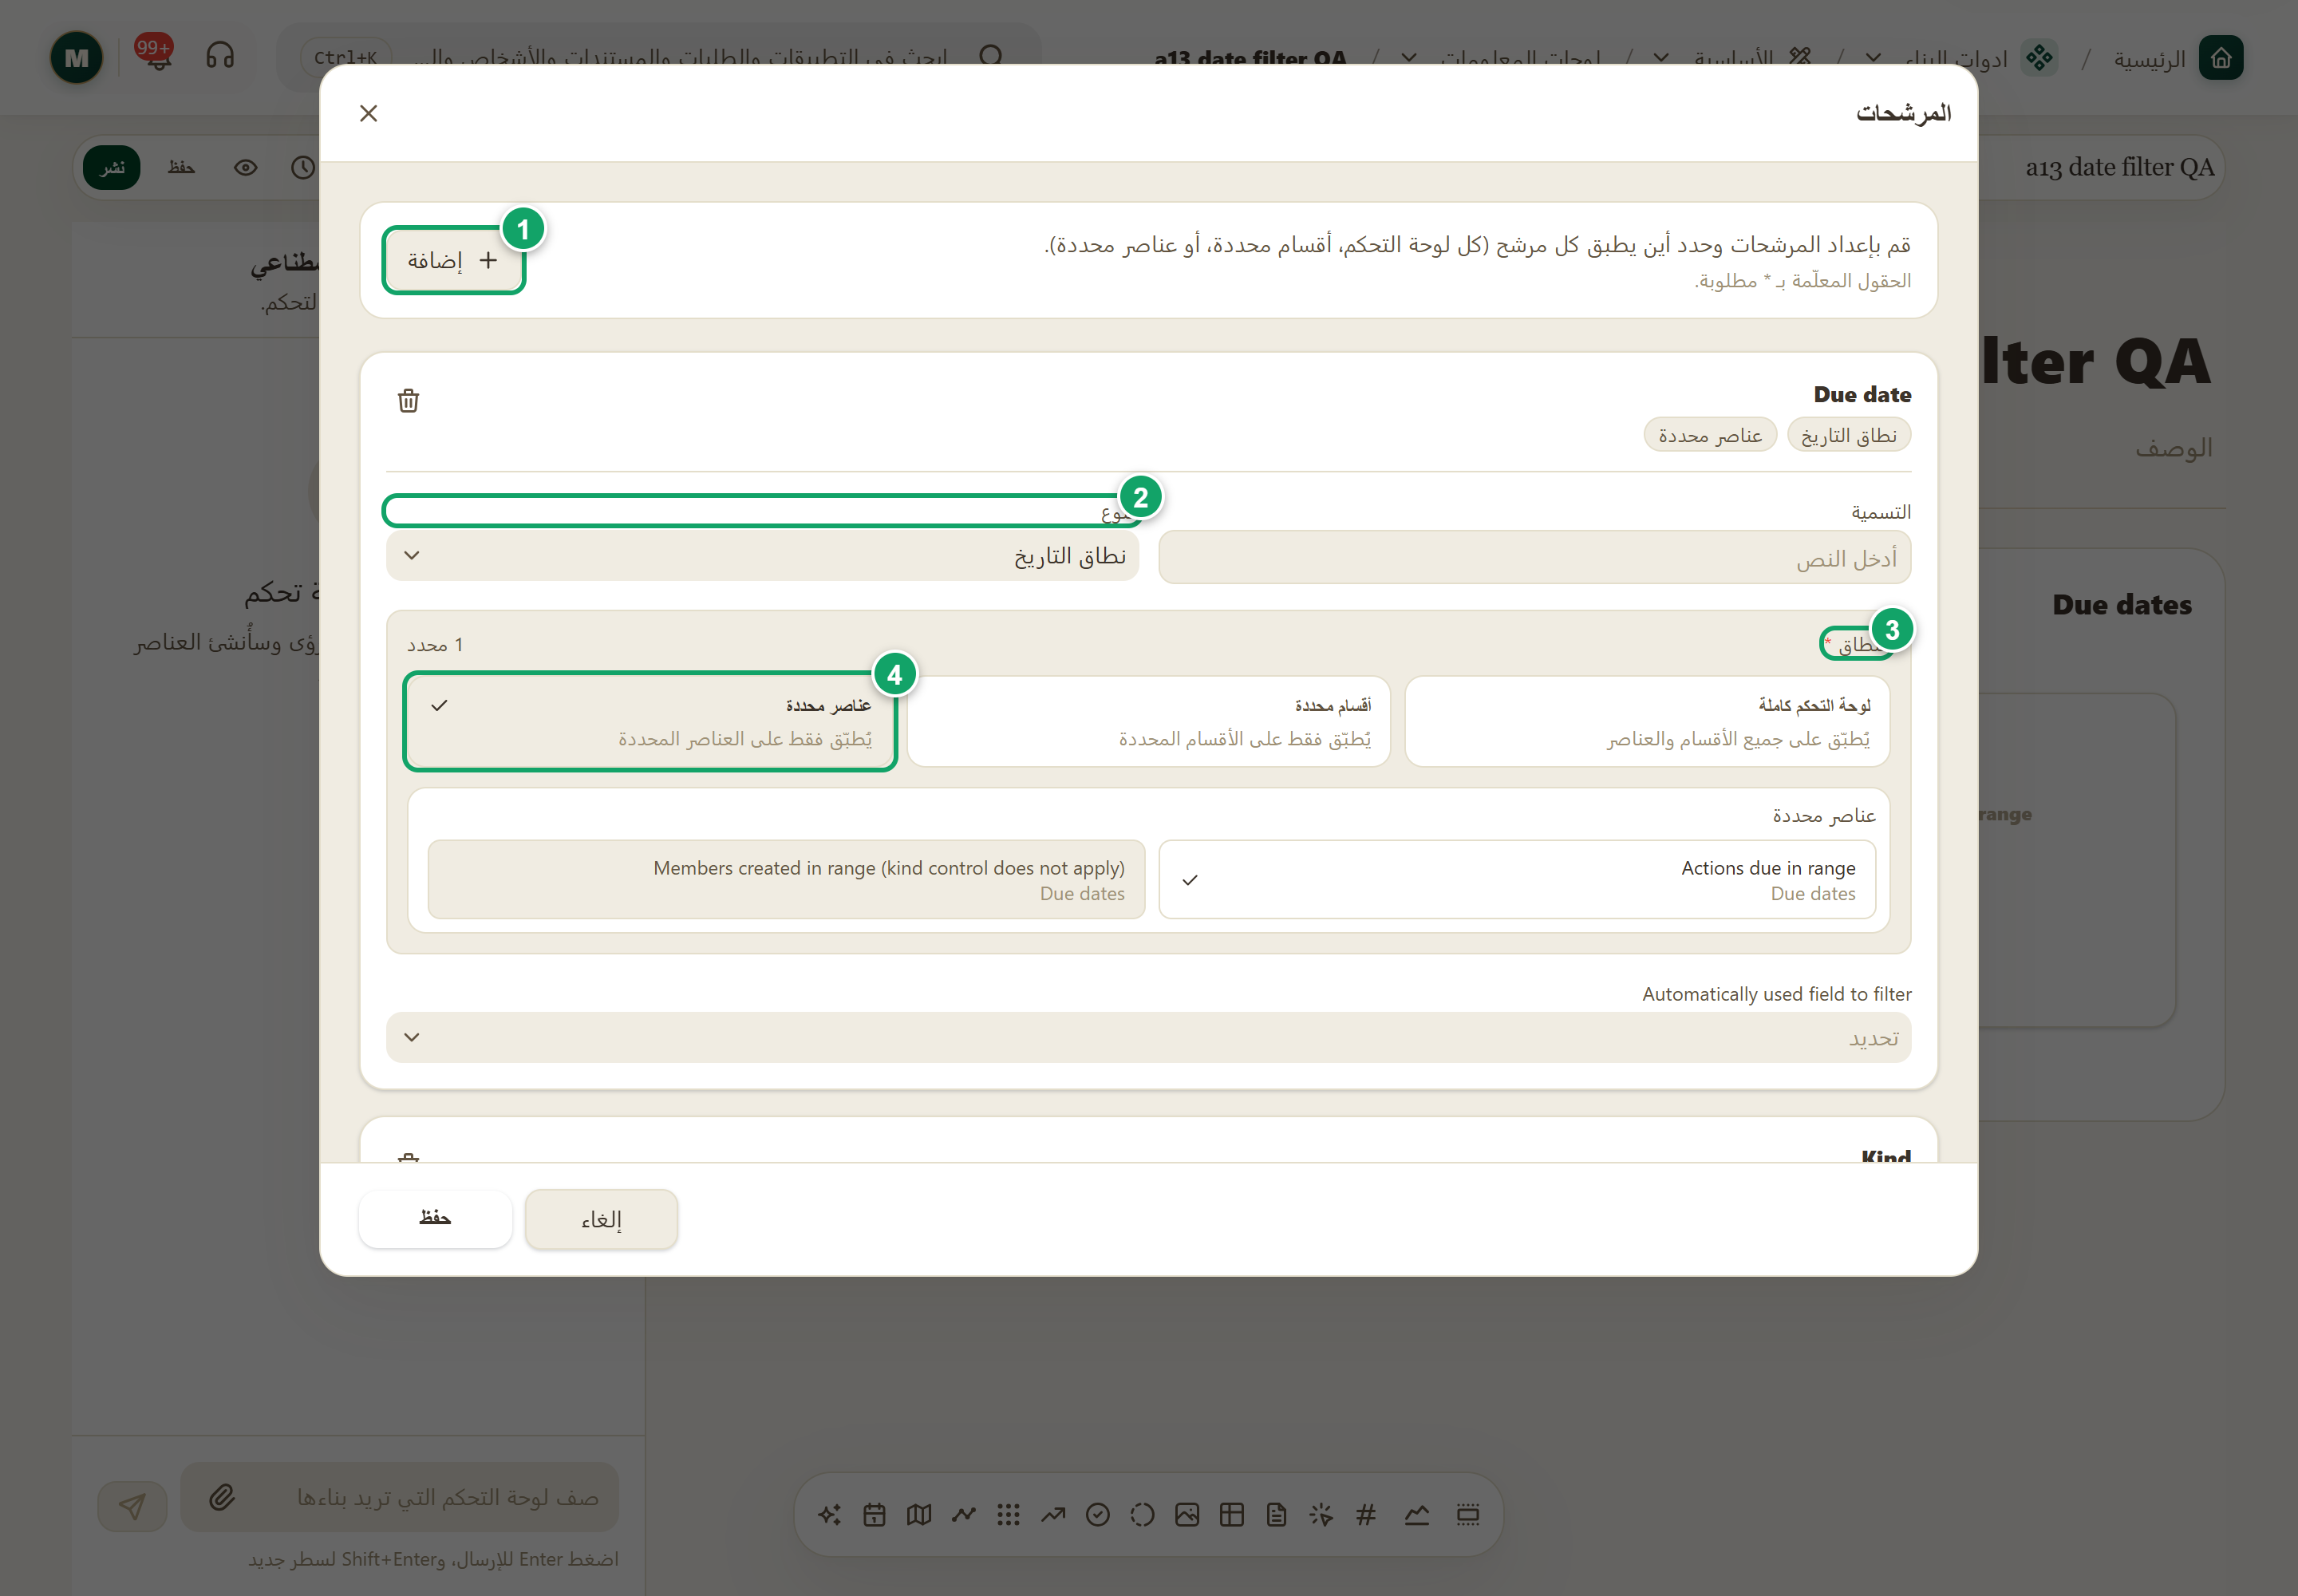
\includegraphics[width=0.95\linewidth,height=0.72\textheight,keepaspectratio]{figures/screens/ch06-dash-filters-ar.png}
\caption{نافذة «المرشحات» في المنشئ}
\label{fig:builder-dashboards-filters-screen}
\shotnote{تعرض الصورة مرشح «نطاق التاريخ» في لوحة اختبار، وقد قُصر نطاقه على عنصر واحد من عنصري القسم. ويبيّن ذلك أن المرشح لا يغيّر إلا العناصر التي يشملها نطاقه، ولو ظهرت كلها في القسم نفسه. ① «إضافة»: يضيف مرشحاً جديداً. ② «النوع»: «نطاق التاريخ» أو «محدد» أو «اختر الحقل». ③ «النطاق»: أين يُطبَّق المرشح. ④ «عناصر محددة»: يطبّقه على العناصر التي تختارها تحته.}
\end{figure}

\begin{table}[H]
\centering
\caption{إعدادات المرشح}
\label{tab:builder-dashboards-filters-fields}
\begin{tabularx}{\linewidth}{R{3.6cm} Y}
\rcHeaderRow
\thh{الإعداد} & \thh{المعنى}\\
«نطاق التاريخ» & تختار حقل التاريخ أو حقوله في كل نوع سجلات، فيقصر المرشح السجلات على الفترة التي يختارها المشاهد.\\
«محدد» & تختار نوع السجلات و«التسمية» و«القيمة الافتراضية (اختياري)»، ويمكن جعله «مطلوب». وتستخدم العناصر قيمته في مرشحاتها عبر معرّف المحدد.\\
«اختر الحقل» & يطابق «الحقل المستهدف» مع خيار يختاره المشاهد. وتأتي الخيارات من «خيارات يدوية» تكتبها، أو «من حقل كيان» من نوع اختيار.\\
«النطاق» & يطبّق المرشح على اللوحة كلها، أو على «أقسام محددة»، أو على «عناصر محددة».\\
\end{tabularx}
\end{table}

\begin{figure}[H]
\centering
\begin{tikzpicture}[node distance=0.5cm]
\node[stepBox] (a) {\RL{اختيار نوع المرشح}};
\node[stepBox,below=of a] (b) {\RL{الحقول أو نوع السجلات}};
\node[stepBox,below=of b] (c) {\RL{تحديد النطاق}};
\node[stepBox,below=of c] (d) {\RL{تجربة المرشح في المعاينة}};
\draw[flowsTo] (a) -- (b);
\draw[flowsTo] (b) -- (c);
\draw[flowsTo] (c) -- (d);
\end{tikzpicture}
\rclegend
\caption{إضافة مرشح للمشاهد}
\label{fig:builder-dashboards-filters-flow}
\shotnote{يضع المخطط النطاق بعد الحقول، لأن المرشح لا يؤثر إلا في العناصر التي تقرأ الحقل الذي ربطته به. ولذلك تأتي التجربة في المعاينة أخيراً، لترى أي العناصر تغيّرت فعلاً عند اختيار فترة أو سجل.}
\end{figure}

\subsection{خطوات العمل والتحقق}
\begin{enumerate}
\item في المنشئ اضغط «المرشحات»، وأضف مرشحاً واختر نوعه.
\item لمرشح «نطاق التاريخ» اختر حقول التاريخ، ولمرشح «محدد» اختر نوع السجلات واكتب «التسمية».
\item اختر «النطاق»: اللوحة كلها، أو «أقسام محددة»، أو «عناصر محددة» ثم حدد الأقسام أو العناصر.
\item اضغط «حفظ»، ثم «معاينة»، وغيّر قيمة المرشح وراقب العناصر.
\end{enumerate}

\textbf{تحقق ومعالجة المشكلة:} يجب أن تتغير أرقام العناصر المشمولة عند تغيير المرشح، وأن يعيدها «مسح الكل» إلى حالها. فإذا رفضت النافذة الحفظ، فأكمل الحقول المميزة، مثل «يرجى اختيار قسم واحد على الأقل.». وإذا لم يتأثر عنصر، فراجع نطاق المرشح والحقل الذي يقرؤه العنصر.

\clearpage
\section{منشئ اللوحة بالذكاء الاصطناعي}
\label{sec:builder-feature-dashboards-ai-builder}

يتيح المنشئ لوحة جانبية تصف فيها اللوحة التي تريدها بكلماتك، فيطرح الذكاء الاصطناعي أسئلة توضيحية ثم يقترح عناصر ومرشحات. ولا يتغير شيء في اللوحة حتى تراجع المقترح وتطبّقه، ثم تبقى النتيجة مسودة تعدّلها وتنشرها كأي لوحة.

\textbf{المسار ومن يستخدمه:} منشئ اللوحة ← اللوحة الجانبية «منشئ لوحات التحكم بالذكاء الاصطناعي»، ويُظهرها الزر الذي يحمل الاسم نفسه أو يخفيها. يستخدمها من يبني اللوحة ويريد بداية سريعة.

\begin{rcnote}[مثال: شركة الأفق]
يكتب مسؤول النظام: «أريد عدد طلبات الزيارة المنتظرة، والطلبات حسب الحالة والفرع، وتقويماً بالمواعيد». فيجيب عن سؤال حول حقل التاريخ، ثم يضغط «تطبيق المقترح» ويراجع العناصر قبل النشر.
\end{rcnote}

\begin{figure}[H]
\centering
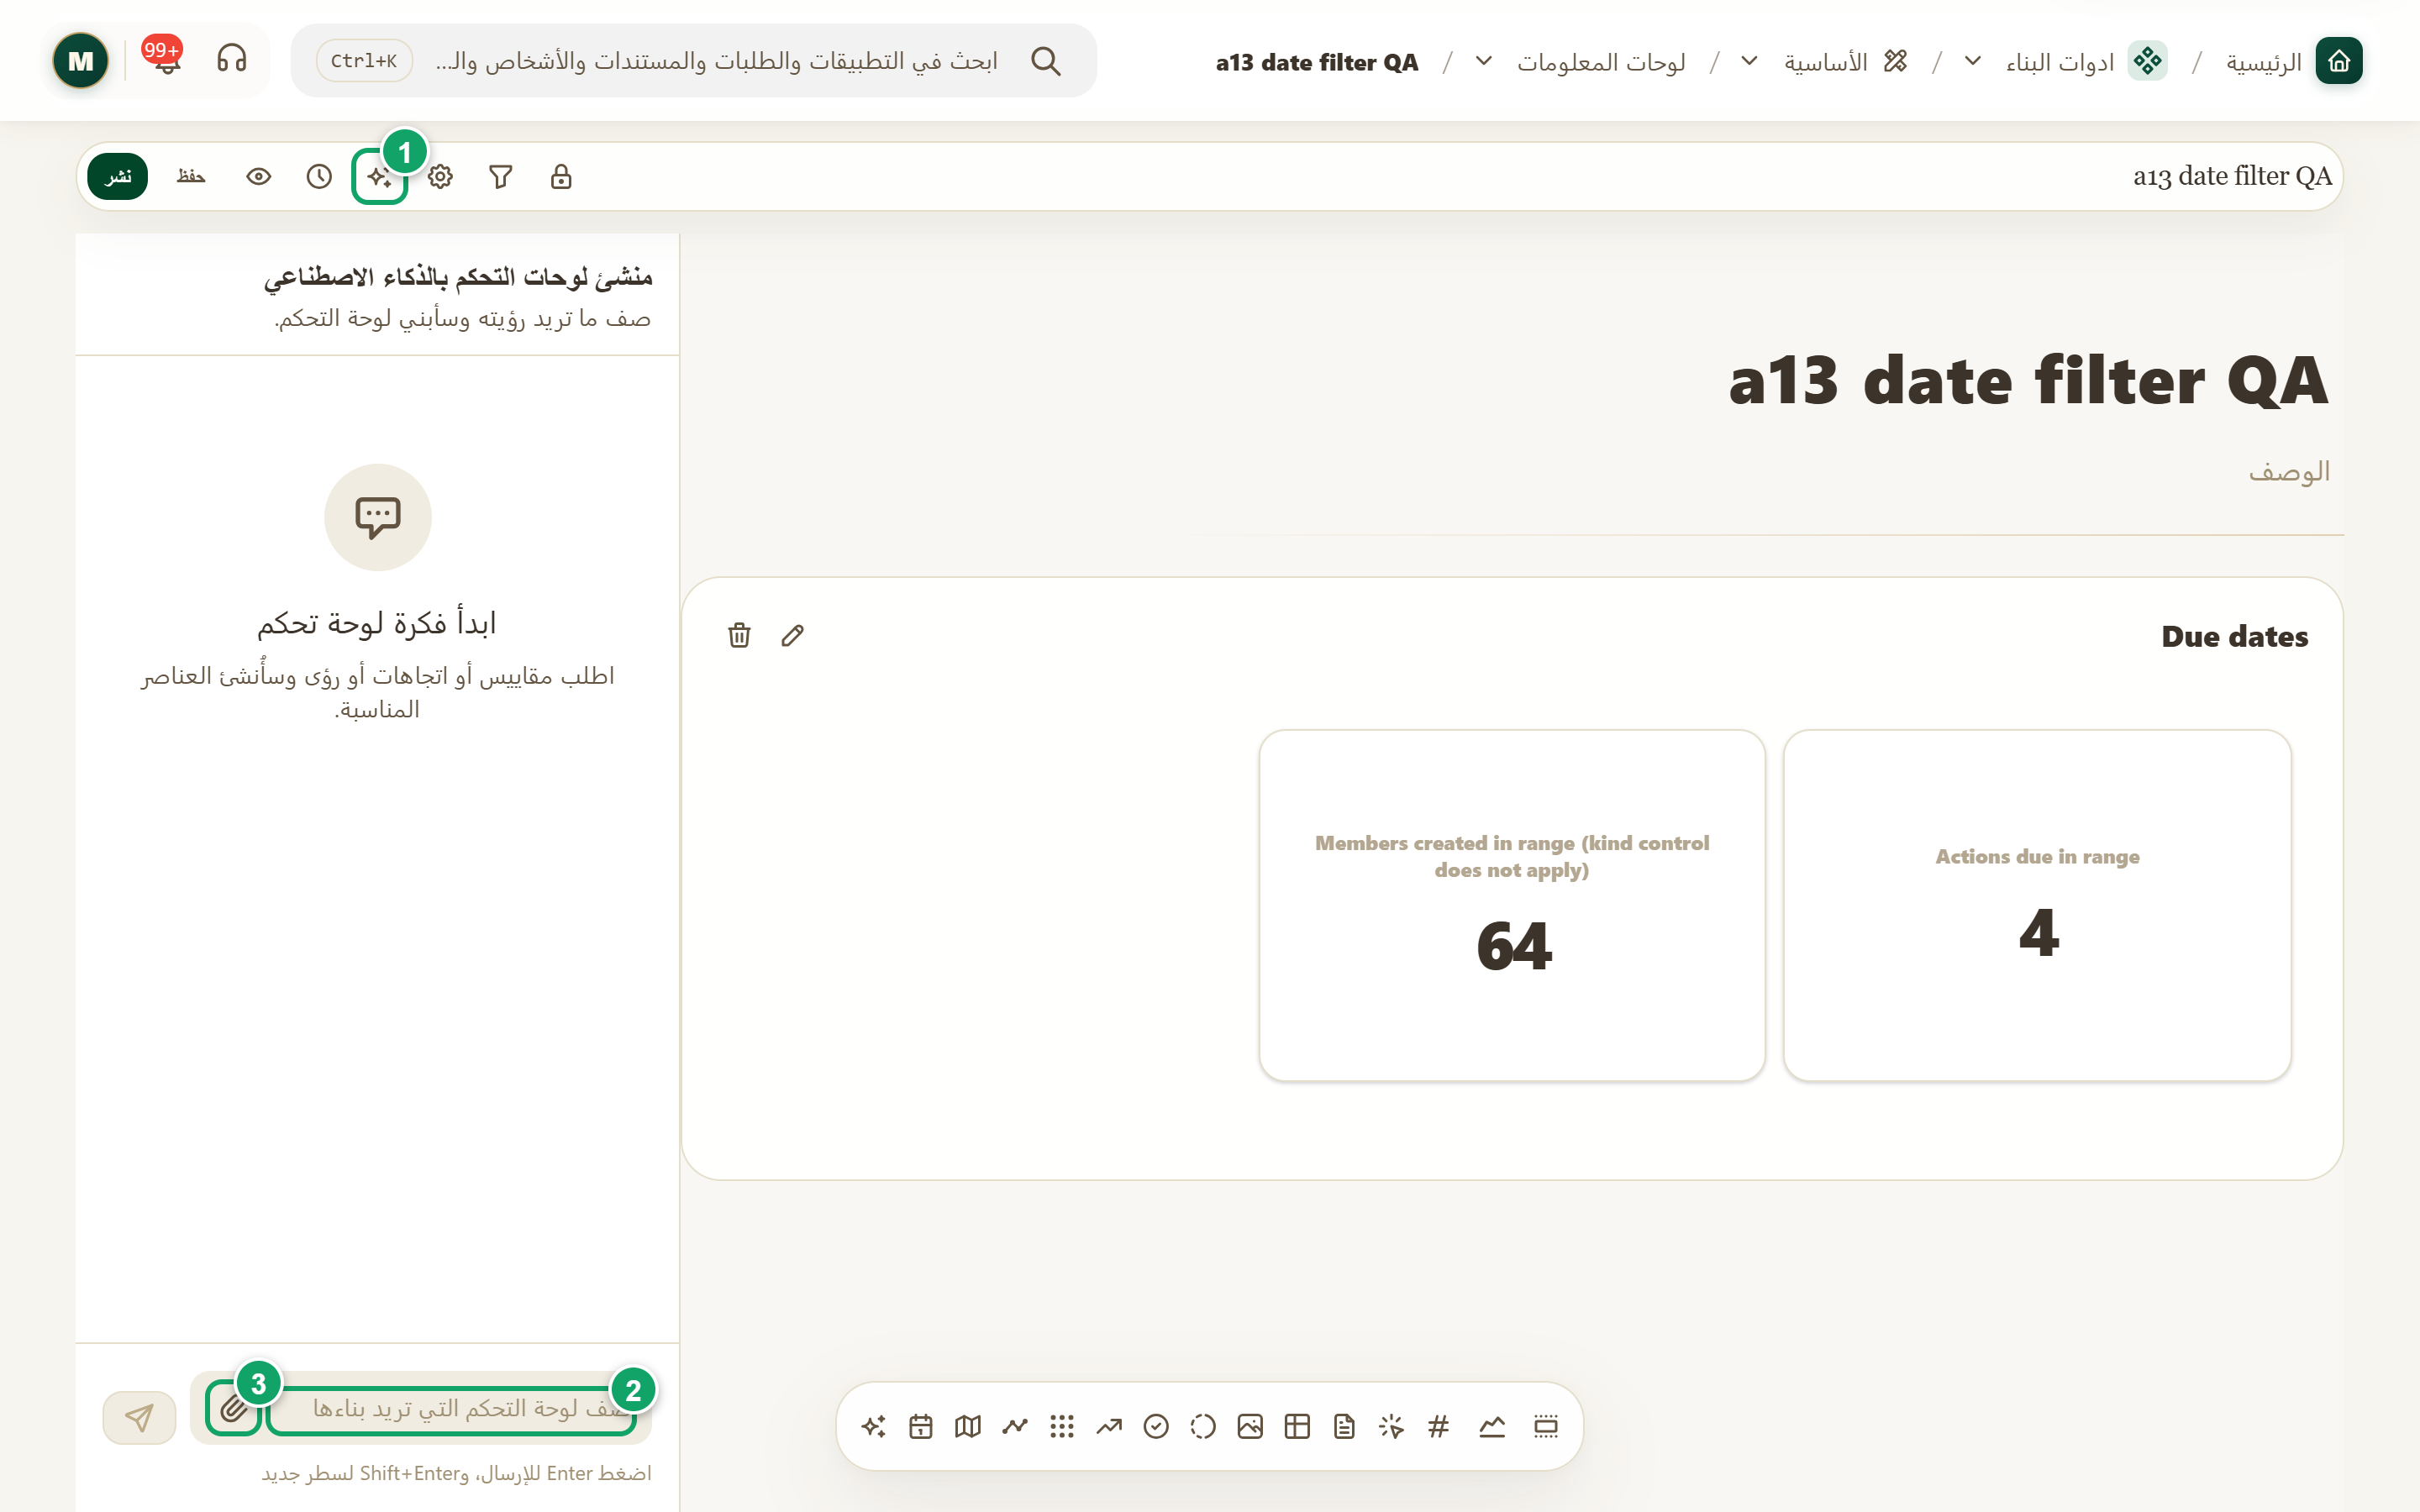
\includegraphics[width=0.95\linewidth,height=0.72\textheight,keepaspectratio]{figures/screens/ch06-dash-ai-builder-ar.png}
\caption{اللوحة الجانبية «منشئ لوحات التحكم بالذكاء الاصطناعي» قبل بدء المحادثة}
\label{fig:builder-dashboards-ai-builder-screen}
\shotnote{تعرض الصورة اللوحة الجانبية ظاهرة في منشئ لوحة اختبار، ولم تبدأ فيها محادثة بعد. ولا يتغير شيء في اللوحة أثناء المحادثة، فالمقترح لا يدخل المسودة إلا عند تطبيقه. ① «منشئ لوحات التحكم بالذكاء الاصطناعي»: يُظهر اللوحة الجانبية أو يخفيها. ② «صف لوحة التحكم التي تريد بناءها»: تكتب فيه طلبك ثم تضغط \en{Enter}. ③ «إرفاق ملف»: يرفق ملفاً يوضح الطلب.}
\end{figure}

\begin{table}[H]
\centering
\caption{مراحل المحادثة}
\label{tab:builder-dashboards-ai-builder-steps}
\begin{tabularx}{\linewidth}{R{3.6cm} Y}
\rcHeaderRow
\thh{المرحلة} & \thh{ما يحدث}\\
الطلب & تكتب في «صف لوحة التحكم التي تريد بناءها» ما تريد رؤيته، ويمكنك «إرفاق ملف» يوضح طلبك.\\
الأسئلة & قد تظهر «يرجى الإجابة على هذه الأسئلة»، فتجيب ثم تضغط «إرسال الإجابات».\\
المقترح & يعرض «ملخص المقترح» عدد العناصر التي يضيفها أو يحدّثها أو يحذفها، وتغييرات المحددات إن وجدت.\\
التطبيق & يضع «تطبيق المقترح» التغييرات في المسودة، وتقبل تغييرات المحددات أو ترفضها بزري «قبول» و«رفض».\\
\end{tabularx}
\end{table}

\begin{figure}[H]
\centering
\begin{tikzpicture}[node distance=0.5cm]
\node[stepBox] (a) {\RL{وصف اللوحة المطلوبة}};
\node[stepBox,below=of a] (b) {\RL{الإجابة عن الأسئلة}};
\node[stepBox,below=of b] (c) {\RL{مراجعة ملخص المقترح}};
\node[stepBox,below=of c] (d) {\RL{تطبيق المقترح}};
\node[stepBox,below=of d] (e) {\RL{مراجعة العناصر ثم النشر}};
\draw[flowsTo] (a) -- (b);
\draw[flowsTo] (b) -- (c);
\draw[flowsTo] (c) -- (d);
\draw[flowsTo] (d) -- (e);
\end{tikzpicture}
\rclegend
\caption{بناء لوحة بمساعدة الذكاء الاصطناعي}
\label{fig:builder-dashboards-ai-builder-flow}
\shotnote{يفصل المخطط بين تطبيق المقترح ونشره، لأن التطبيق يغيّر المسودة فقط. فتراجع كل عنصر ومصدره ومستوى الوصول فيه بعد التطبيق، ثم تنشر عندما تتأكد أن الأرقام صحيحة.}
\end{figure}

\subsection{خطوات العمل والتحقق}
\begin{enumerate}
\item في المنشئ، إذا لم تظهر اللوحة الجانبية، فاضغط «منشئ لوحات التحكم بالذكاء الاصطناعي».
\item اكتب ما تريد رؤيته مع نوع السجلات والفترة، ثم اضغط \en{Enter} للإرسال.
\item أجب عن الأسئلة إن ظهرت واضغط «إرسال الإجابات»، ثم راجع «ملخص المقترح».
\item اضغط «تطبيق المقترح»، ثم افتح كل عنصر وراجع مصدر بياناته و«مستوى الوصول» قبل «حفظ» و«نشر».
\end{enumerate}

\textbf{تحقق ومعالجة المشكلة:} يجب أن يتحول الزر إلى «تم التطبيق» وأن تظهر العناصر في المنشئ. فإذا لم يطابق المقترح ما أردت، فاكتب طلباً أدق بدلاً من تطبيقه. وإذا ظهر «خطأ في العنصر» في عنصر مقترح، فاستخدم «إرسال الخطأ إلى الذكاء الاصطناعي» ليصححه، أو اضبط العنصر يدوياً.

\clearpage
\section{المعاينة والنشر والإصدارات}
\label{sec:builder-feature-dashboards-publish}

يحفظ المنشئ عملك مسودةً لا يراها المشاهدون. وتعرض «معاينة» اللوحة كما ستظهر لهم، ثم يُنشئ «نشر» إصداراً جديداً يحل محل الإصدار المنشور. ويحتفظ «سجل الإصدارات» بالإصدارات السابقة، فتعود إلى أي منها عند الحاجة.

\textbf{المسار ومن يستخدمه:} منشئ اللوحة ← «معاينة» أو «نشر» أو «الإصدارات». يستخدمها من يملك صلاحية تعديل اللوحة.

\begin{rcnote}[مثال: شركة الأفق]
يعاين مسؤول النظام لوحة «متابعة الزيارات» فيرى أن عدد الطلبات المنتظرة يطابق ما في القائمة، فيضغط «نشر». وبعد أسبوع يحذف عنصراً بالخطأ، فيستعيد الإصدار السابق من «سجل الإصدارات».
\end{rcnote}

\begin{figure}[H]
\centering
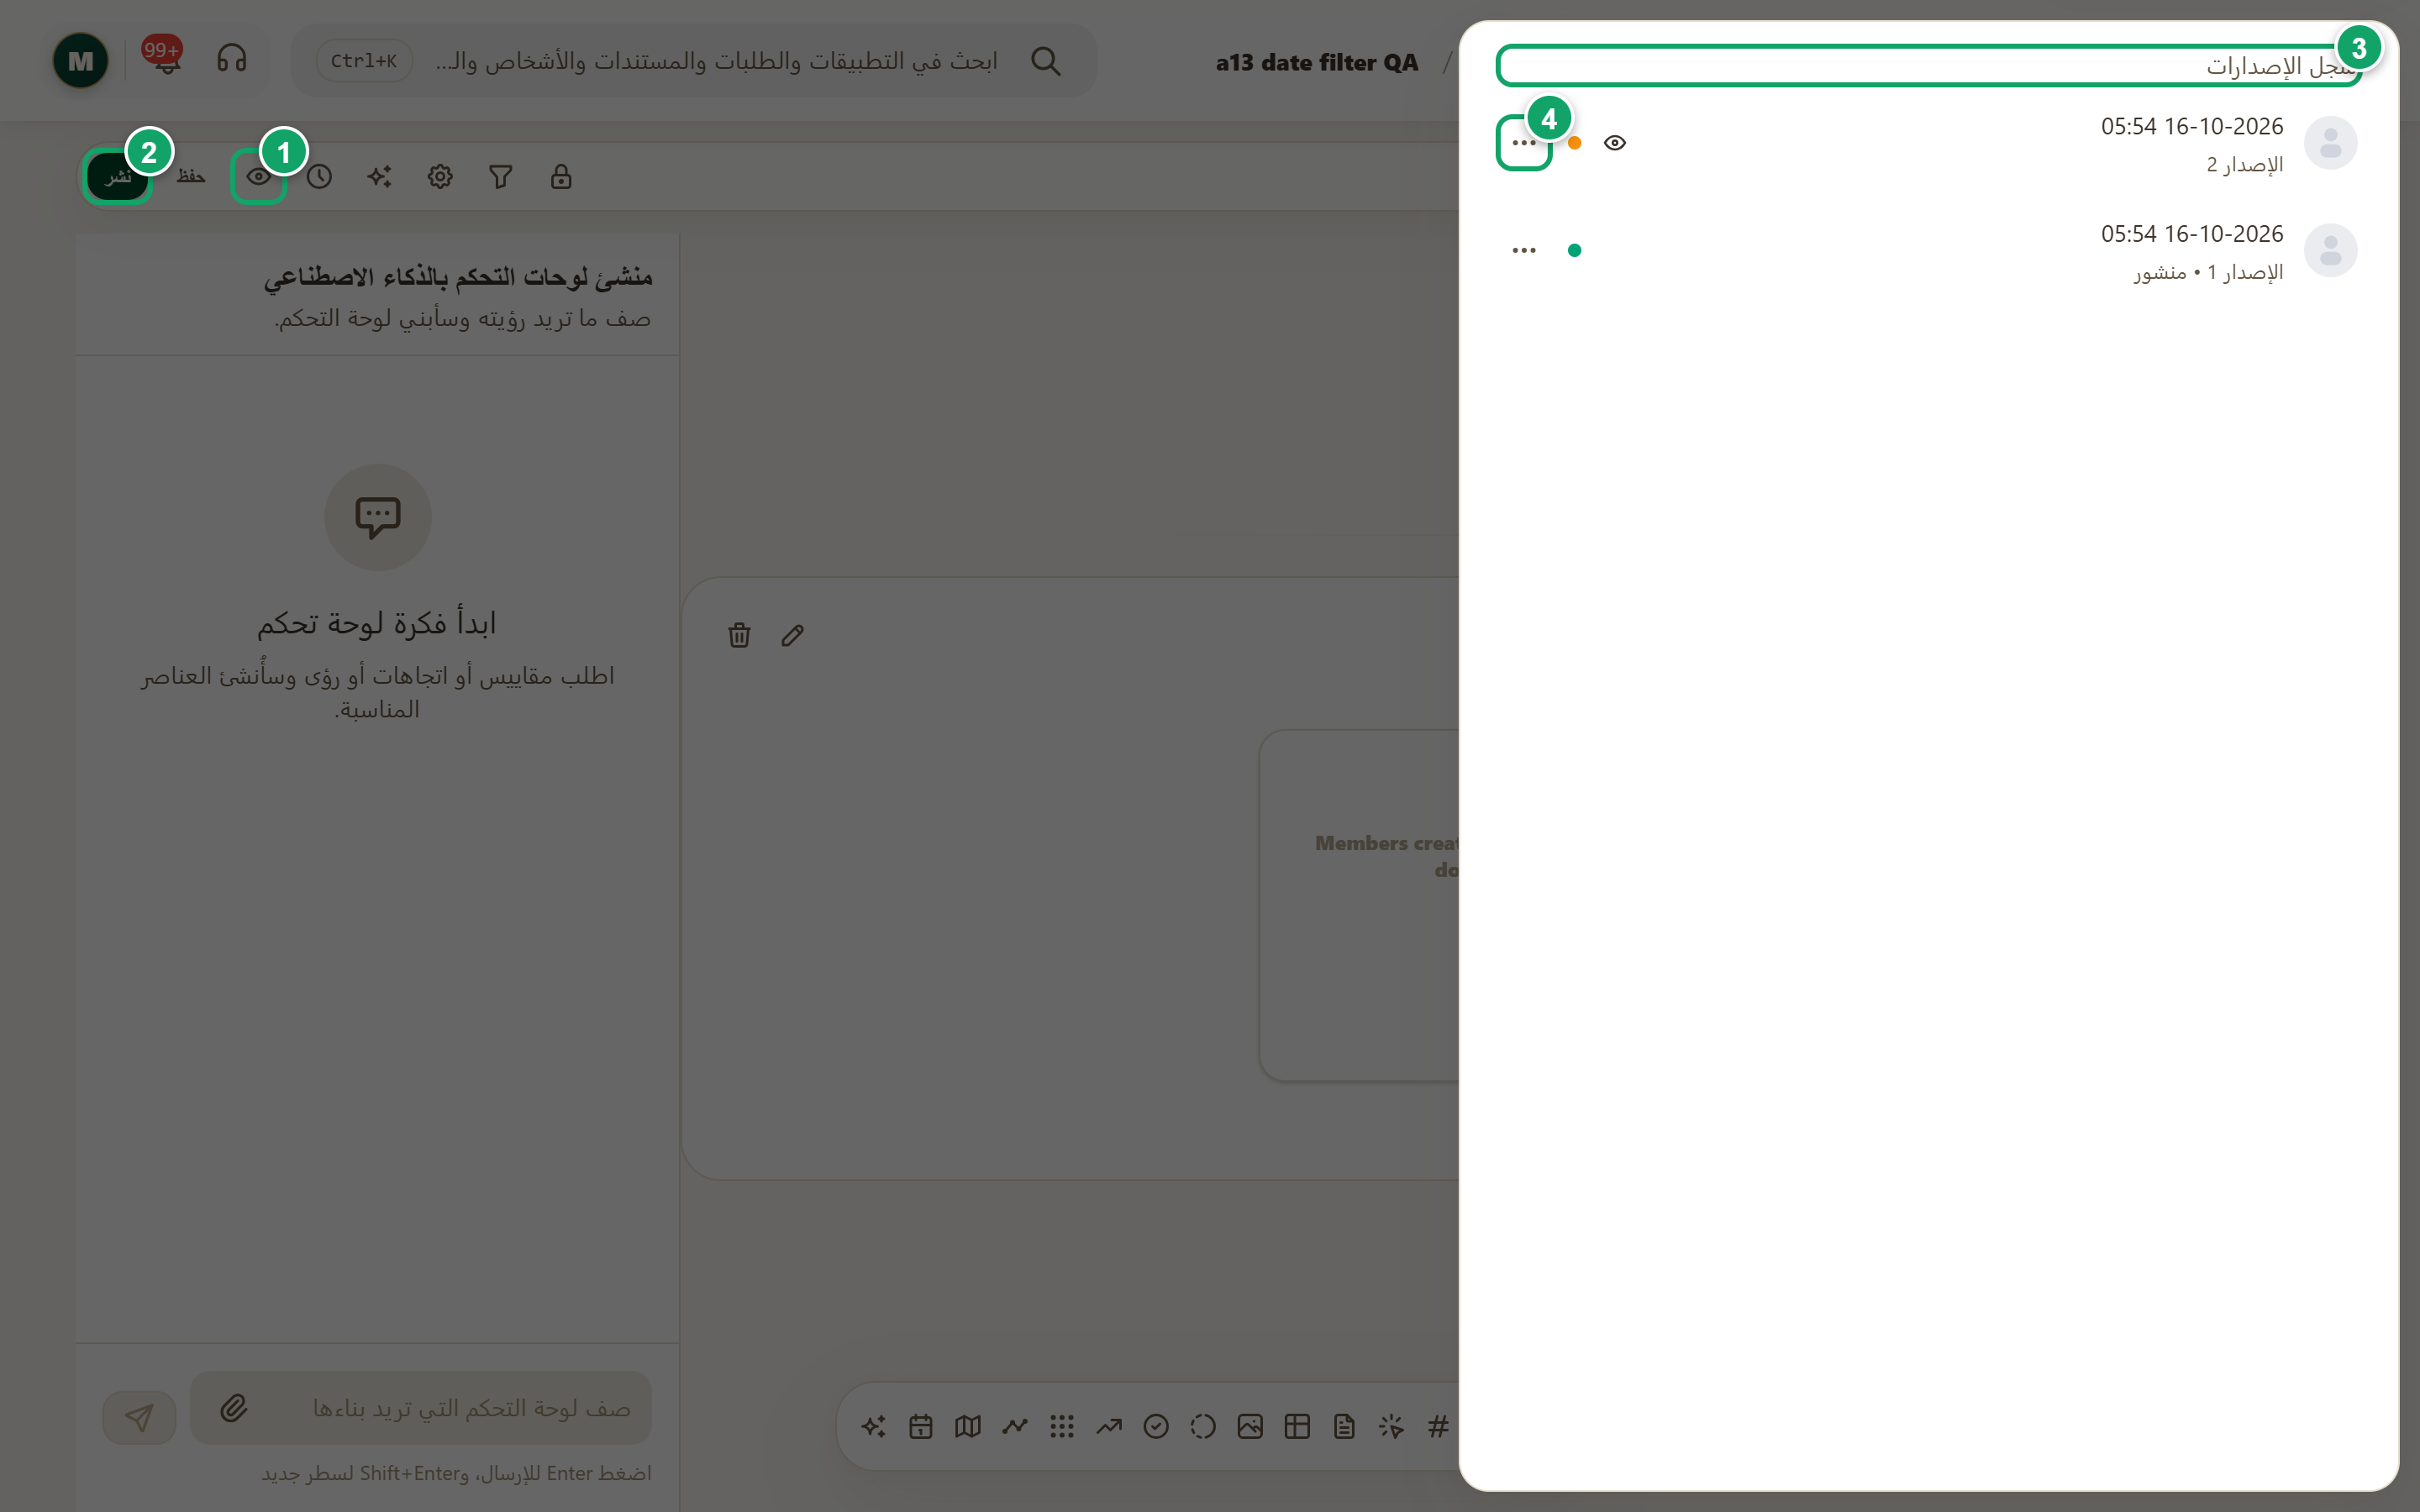
\includegraphics[width=0.95\linewidth,height=0.72\textheight,keepaspectratio]{figures/screens/ch06-dash-versions-ar.png}
\caption{نافذة «سجل الإصدارات» مع زري المعاينة والنشر}
\label{fig:builder-dashboards-publish-screen}
\shotnote{تعرض الصورة سجل إصدارات لوحة اختبار فيه إصداران: الأول منشور بنقطة خضراء، والثاني مسودة أحدث بنقطة برتقالية لم تُنشر بعد. ويبيّن ذلك أن ما يراه المشاهدون هو الإصدار المنشور، لا آخر ما حُفظ في المنشئ. ① «معاينة»: يعرض اللوحة كما يراها المشاهد. ② «نشر»: يحفظ المسودة وينشرها إصداراً جديداً. ③ «سجل الإصدارات»: قائمة الإصدارات بأرقامها وتواريخها. ④ «المزيد من الخيارات»: قائمة الإصدار التي فيها «عرض» و«استعادة».}
\end{figure}

\begin{table}[H]
\centering
\caption{أدوات المعاينة والنشر}
\label{tab:builder-dashboards-publish-tools}
\begin{tabularx}{\linewidth}{R{3.6cm} Y}
\rcHeaderRow
\thh{الأداة} & \thh{ما تفعله}\\
«معاينة» & تعرض اللوحة بالبيانات الحقيقية دون أدوات التعديل، مع شريط «معاينة لوحة المعلومات»، وتعود منها بزر «خروج من المعاينة».\\
«حفظ» & يحفظ المسودة دون أن يغيّر ما يراه المشاهدون.\\
«نشر» & يحفظ ما في المنشئ ثم ينشره إصداراً جديداً، وتظهر رسالة «تم نشر لوحة المعلومات بنجاح».\\
«سجل الإصدارات» & يعرض كل إصدار برقمه وتاريخه، ويُكتب بجانب الإصدار المنشور «منشور» مع نقطة خضراء، وتميّز النقطة البرتقالية المسودة. ومن قائمة الإصدار تختار «عرض»، أو «تعديل كمسودة»، أو «استعادة».\\
\end{tabularx}
\end{table}

\begin{rcwarn}[الاستعادة تستبدل المسودة الحالية]
يستبدل «تعديل كمسودة» و«استعادة» المسودة الحالية بالإصدار الذي اخترته، فتضيع التعديلات غير المنشورة. ولا يرى المشاهدون الإصدار المستعاد حتى تنشره.
\end{rcwarn}

\begin{figure}[H]
\centering
\begin{tikzpicture}[node distance=0.5cm]
\node[stepBox] (a) {\RL{حفظ المسودة}};
\node[stepBox,below=of a] (b) {\RL{معاينة ومقارنة بسجلات معروفة}};
\node[stepBox,below=of b] (c) {\RL{نشر إصدار جديد}};
\node[stepBox,below=of c] (d) {\RL{استعادة إصدار سابق عند الخطأ}};
\draw[flowsTo] (a) -- (b);
\draw[flowsTo] (b) -- (c);
\draw[flowsTo] (c) -- (d);
\end{tikzpicture}
\rclegend
\caption{من المسودة إلى إصدار منشور}
\label{fig:builder-dashboards-publish-flow}
\shotnote{يضع المخطط المقارنة بسجلات معروفة قبل النشر، لأن الرقم الخاطئ في لوحة يقود إلى قرار خاطئ؛ فإذا كنت تعرف أن خمسة طلبات تنتظر، فيجب أن يعرض العنصر خمسة. وتأتي الاستعادة أخيراً بوصفها طريق العودة إذا ظهر خطأ بعد النشر.}
\end{figure}

\subsection{خطوات العمل والتحقق}
\begin{enumerate}
\item اضغط «حفظ»، ثم «معاينة»، وقارن أرقام العناصر بسجلات تعرفها.
\item اضغط «خروج من المعاينة» وصحّح ما يلزم، ثم اضغط «نشر».
\item لاستعادة إصدار، اضغط «الإصدارات»، وافتح قائمة الإصدار واختر «استعادة» ثم أكّد.
\item انشر اللوحة مرة أخرى ليصل الإصدار المستعاد إلى المشاهدين.
\end{enumerate}

\textbf{تحقق ومعالجة المشكلة:} يجب أن يظهر في «سجل الإصدارات» إصدار جديد بحالة «منشور». فإذا ظهرت «فشل نشر لوحة المعلومات. يرجى المحاولة مرة أخرى.»، فاحفظ أولاً ثم أعد النشر. وإذا رأى المشاهدون النسخة القديمة، فتأكد أنك نشرت بعد آخر تعديل.

\clearpage
\section{عرض اللوحة وتصديرها}
\label{sec:builder-feature-dashboards-viewing}

يفتح المشاهد اللوحة المنشورة من التنقل أو من قائمة «لوحات المعلومات»، فيرى الإصدار المنشور بحسب صلاحياته. ويستطيع تغيير المرشحات التي أعدّها صاحب اللوحة، وتصدير بيانات جدول، وتصدير اللوحة كلها تقريراً بصيغة \en{PDF}.

\textbf{المسار ومن يستخدمه:} قسم التطبيق الذي تظهر فيه اللوحة، أو «لوحات المعلومات» ← قائمة البطاقة ← «عرض». يستخدمها كل من مُنح الوصول إلى اللوحة.

\begin{rcnote}[مثال: شركة الأفق]
تفتح سارة الخطيب لوحة «متابعة الزيارات» من «خدمات الفروع»، وتختار فرع حلب في المرشح، ثم تضغط «تصدير PDF» لترفق التقرير بمحضر الاجتماع الشهري.
\end{rcnote}

\begin{figure}[H]
\centering
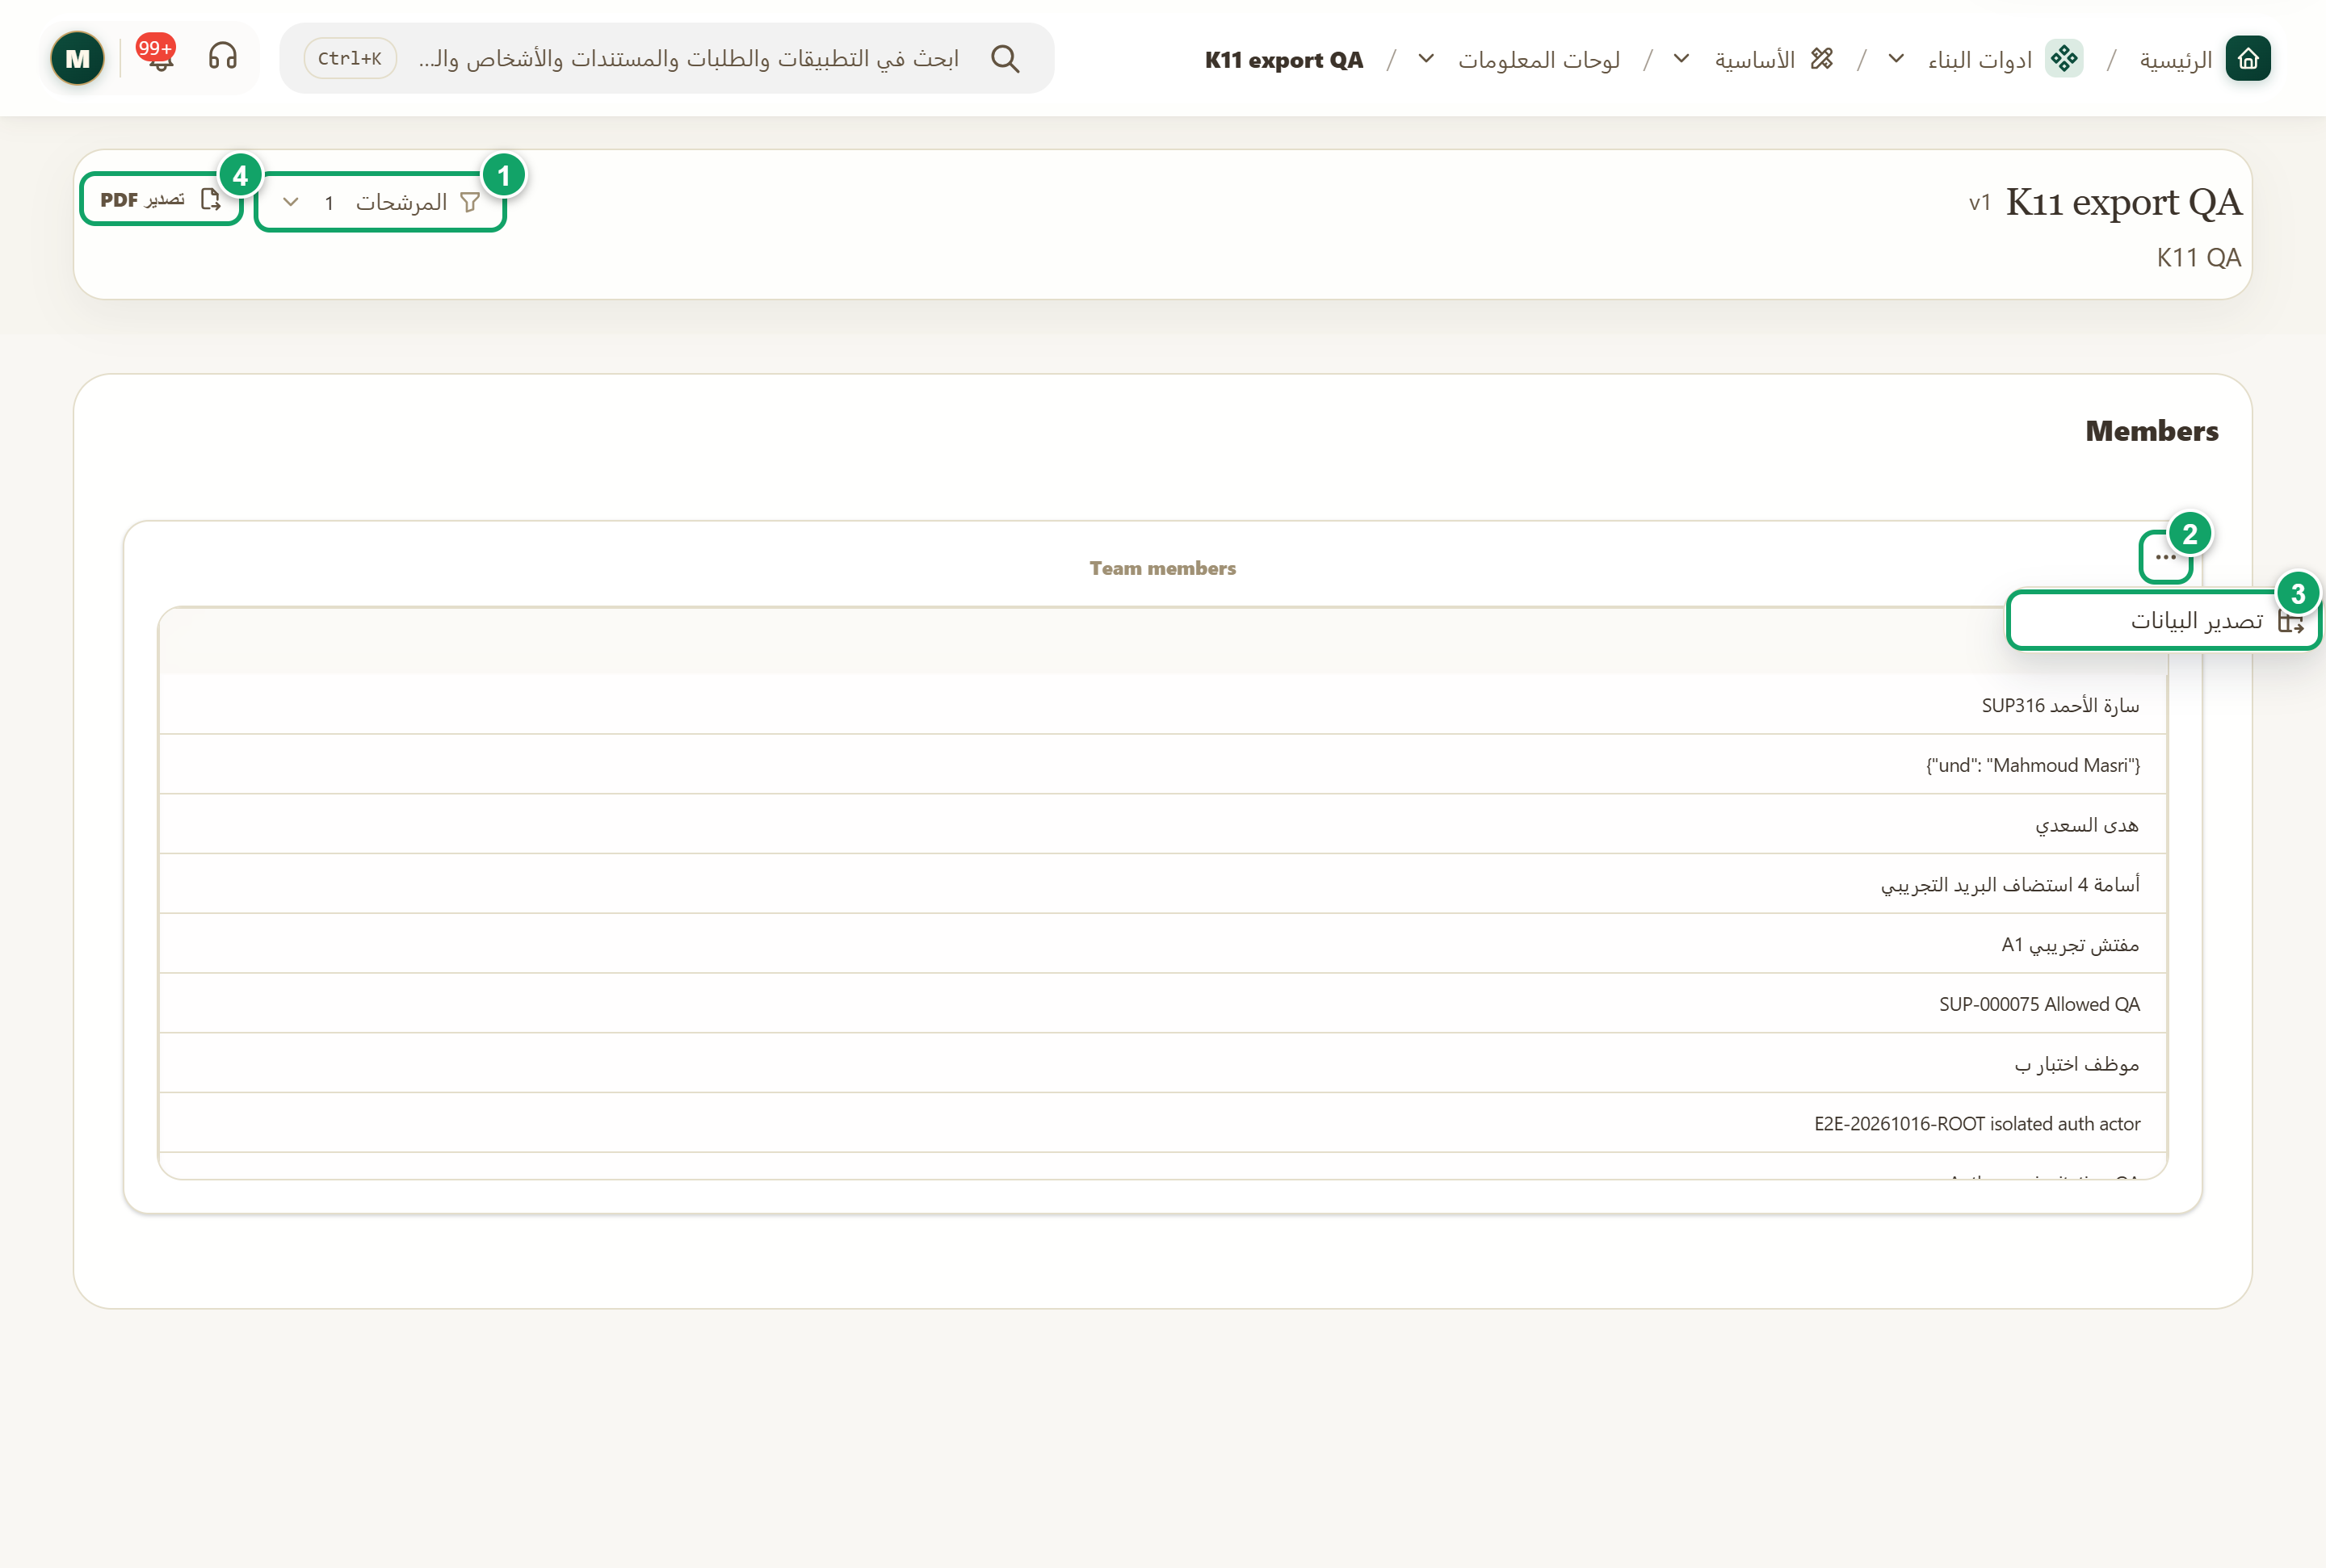
\includegraphics[width=0.95\linewidth,height=0.72\textheight,keepaspectratio]{figures/screens/ch06-dash-view-ar.png}
\caption{لوحة منشورة في وضع العرض مع قائمة «خيارات العنصر»}
\label{fig:builder-dashboards-viewing-screen}
\shotnote{تعرض الصورة لوحة اختبار منشورة فيها جدول كيان، وقد فُتحت قائمة الجدول دون تنفيذ أي تصدير. ويبيّن الرقم بجانب «المرشحات» عدد المرشحات المضبوطة، وهي تنطبق على البيانات المصدّرة أيضاً. ① «المرشحات»: يغيّر بها المشاهد الفترة أو السجل. ② «خيارات العنصر»: زر النقاط في زاوية الجدول. ③ «تصدير البيانات»: يصدّر سجلات الجدول بالمرشحات الحالية. ④ «تصدير PDF»: يجهّز تقريراً من اللوحة كلها.}
\end{figure}

\begin{table}[H]
\centering
\caption{ما يستطيع المشاهد فعله}
\label{tab:builder-dashboards-viewing-actions}
\begin{tabularx}{\linewidth}{R{3.6cm} Y}
\rcHeaderRow
\thh{الإجراء} & \thh{كيف يتم}\\
«المرشحات» & يغيّر المشاهد الفترة أو السجل أو الخيار، فتتغير العناصر المشمولة، ويعيدها «مسح الكل» إلى القيم الافتراضية.\\
«تصدير البيانات» & يظهر في قائمة «خيارات العنصر» لجداول الكيانات لمن يملك صلاحية التصدير، ويُصدّر السجلات بالمرشحات الحالية. وقد يُجهَّز الملف في الخلفية ثم يصل إشعار عند جاهزيته.\\
«تصدير PDF» & يجهّز تقريراً من كل عناصر اللوحة بالمرشحات الحالية، ثم يفتحه في تبويب جديد مع نافذة الطباعة لحفظه بصيغة \en{PDF}.\\
\end{tabularx}
\end{table}

\begin{figure}[H]
\centering
\begin{tikzpicture}[node distance=0.5cm]
\node[stepBox] (a) {\RL{فتح اللوحة المنشورة}};
\node[stepBox,below=of a] (b) {\RL{ضبط المرشحات}};
\node[stepBox,below=of b] (c) {\RL{تصدير البيانات من جدول}};
\node[stepBox,below=of c] (d) {\RL{تصدير PDF للوحة كلها}};
\draw[flowsTo] (a) -- (b);
\draw[flowsTo] (b) -- (c);
\draw[flowsTo] (c) -- (d);
\end{tikzpicture}
\rclegend
\caption{من العرض إلى التقرير}
\label{fig:builder-dashboards-viewing-flow}
\shotnote{يضع المخطط ضبط المرشحات قبل التصدير، لأن الملف والتقرير يحملان الفترة والسجلات المختارة وقت التصدير. وبذلك يطابق ما تشاركه ما رأيته على الشاشة.}
\end{figure}

\subsection{خطوات العمل والتحقق}
\begin{enumerate}
\item افتح اللوحة من قسم التطبيق، أو اختر «عرض» من قائمة بطاقتها.
\item اضبط «المرشحات» على الفترة والسجل المطلوبين.
\item لتصدير جدول، اضغط زر النقاط في زاويته واختر «تصدير البيانات».
\item لتقرير كامل، اضغط «تصدير PDF»، ثم احفظ الملف من نافذة الطباعة.
\end{enumerate}

\textbf{تحقق ومعالجة المشكلة:} يجب أن يعرض التقرير العناصر بالمرشحات التي اخترتها. فإذا ظهرت «يرجى السماح بالنوافذ المنبثقة لفتح تقرير PDF في تبويب جديد.»، فاسمح بها في المتصفح وأعد المحاولة. وإذا لم يظهر «تصدير البيانات»، فأنت لا تملك صلاحية التصدير أو العنصر ليس جدول كيان. وإذا ظهرت «لم يتم نشر لوحة المعلومات بعد»، فاطلب من صاحبها نشرها.

\clearpage
\section{الصفحات}
\label{sec:builder-feature-pages}

الصفحة تضع لوحة معلومات محفوظة من مساحة التحليلات بالذكاء الاصطناعي (\en{DB Genie}) داخل قسم في تطبيق، فتظهر للأعضاء عنصراً في القائمة. وهي الطريقة لمشاركة لوحة صنعتها في «لوحات معلومات الذكاء الاصطناعي» مع الفريق.

\textbf{المسار ومن يستخدمه:} «ادوات البناء» ← «الأساسية» ← «الصفحات». تظهر لمالك المؤسسة ومسؤولها فقط.

\begin{rcnote}[مثال: شركة الأفق]
يصنع مسؤول النظام لوحة تحليل لمدد إنجاز الزيارات في مساحة الذكاء الاصطناعي، ثم ينشرها صفحةً في قسم «الزيارات» داخل «خدمات الفروع» لتراها سارة الخطيب. وتبدأ الصفحة من ①.
\end{rcnote}

\begin{figure}[H]
\centering
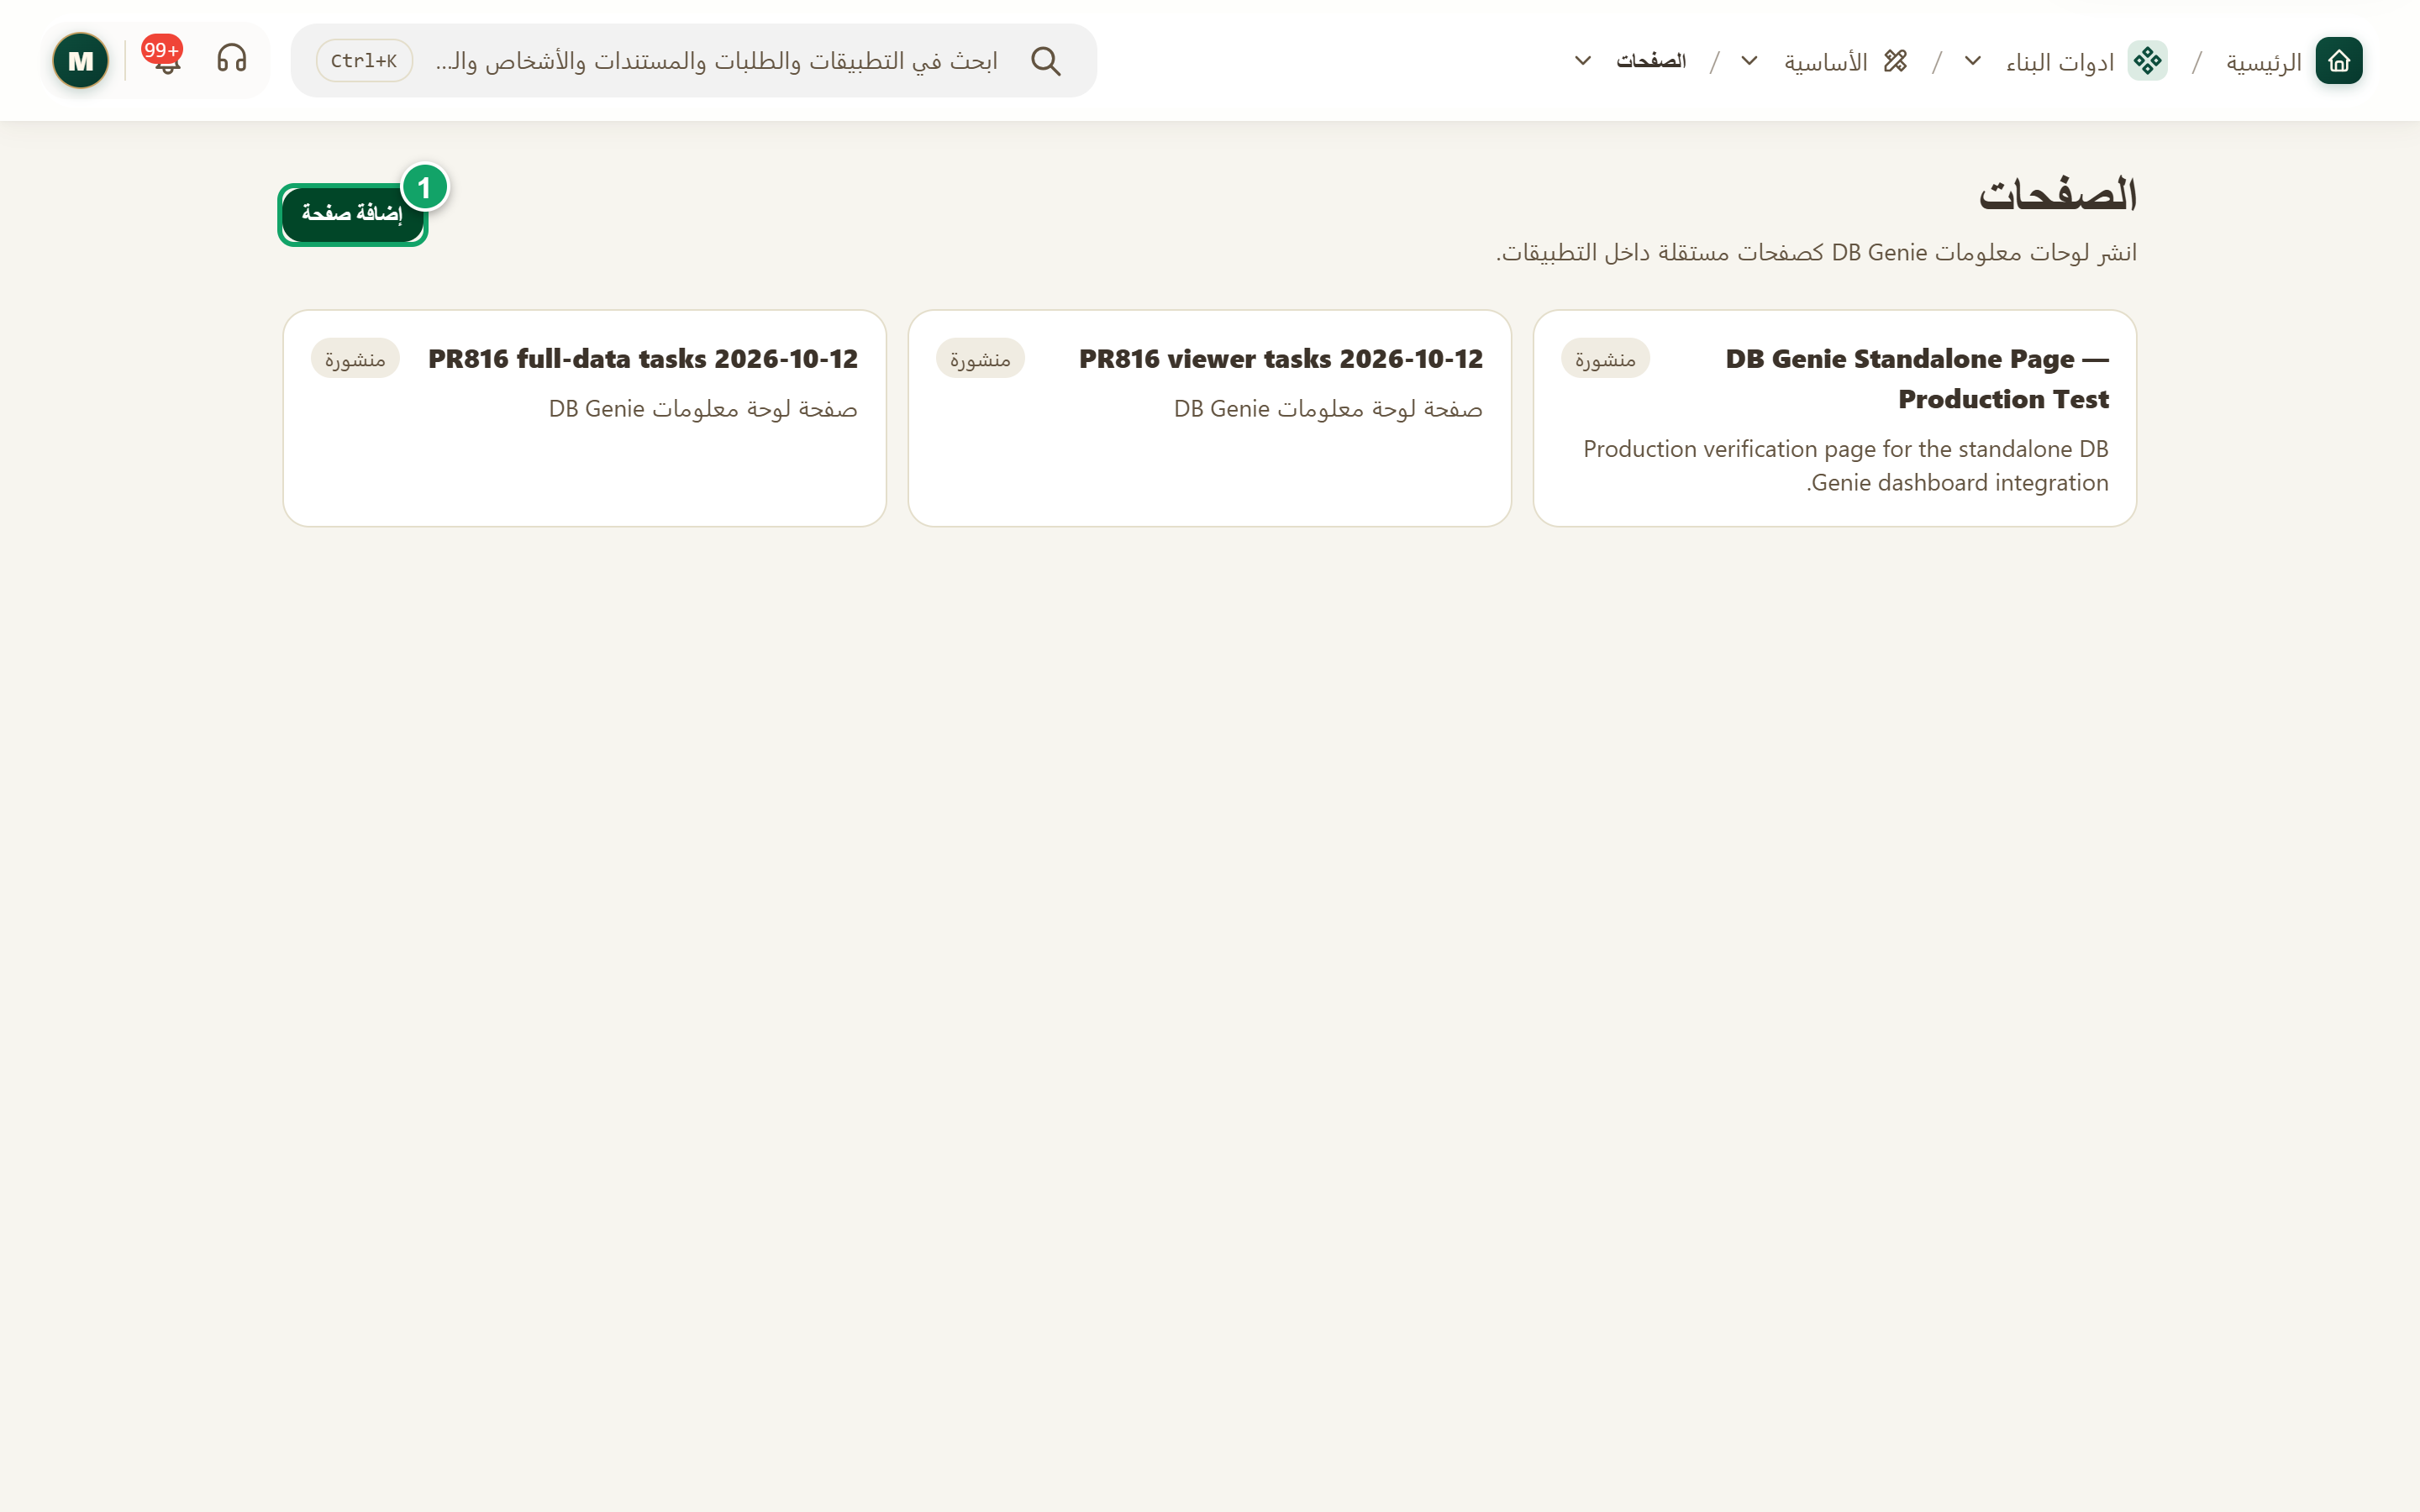
\includegraphics[width=0.95\linewidth,height=0.72\textheight,keepaspectratio]{figures/screens/ch06-pages-ar.png}
\caption{صفحة «الصفحات»}
\label{fig:builder-pages-screen}
\shotnote{تعرض الصفحة الصفحات المستقلة المنشورة في التطبيقات، وهي هنا صفحات اختبار. ① «إضافة صفحة»: تبدأ صفحة جديدة تختار لها اللوحة والتطبيق والقسم.}
\end{figure}


\begin{table}[H]
\centering
\caption{حقول الصفحة}
\label{tab:builder-pages-data}
\begin{tabularx}{\linewidth}{R{3.6cm} Y}
\rcHeaderRow
\thh{الحقل} & \thh{المعنى}\\
العنوان والوصف & اسم الصفحة كما يظهر في القائمة، ووصف قصير.\\
التطبيق والقسم & المكان الذي تظهر فيه الصفحة في التنقل.\\
لوحة معلومات DB Genie & لوحة محفوظة تختارها بزر «اختيار لوحة معلومات».\\
البيانات المعروضة & «بصلاحيات المشاهد» وهو الأكثر أماناً، أو بيانات المؤسسة بحماية، أو بيانات المؤسسة كاملة دون تحقق من نطاق المشاهد.\\
الحالة & «مسودة» أو «منشورة» أو «مؤرشفة». ولا تظهر الصفحة في التنقل إلا وهي منشورة.\\
\end{tabularx}
\end{table}

\begin{figure}[H]
\centering
\begin{tikzpicture}[node distance=0.5cm]
\node[stepBox] (a) {\RL{لوحة في مساحة الذكاء الاصطناعي}};
\node[stepBox,below=of a] (b) {\RL{إضافة صفحة واختيار اللوحة}};
\node[stepBox,below=of b] (c) {\RL{الحالة: منشورة}};
\node[stepBox,below=of c] (d) {\RL{منح صلاحية العرض للأدوار}};
\draw[flowsTo] (a) -- (b);
\draw[flowsTo] (b) -- (c);
\draw[flowsTo] (c) -- (d);
\end{tikzpicture}
\rclegend
\caption{من لوحة خاصة إلى صفحة للفريق}
\label{fig:builder-pages-flow}
\shotnote{يبيّن المخطط أن نشر الصفحة وحده لا يكفي ليراها الأعضاء، بل يحتاج كل دور إلى صلاحية عرض الصفحة في إعدادات الأدوار. وتبقى اللوحة الأصلية كما هي، فحذف الصفحة لا يحذف اللوحة.}
\end{figure}

\subsection{خطوات العمل والتحقق}
\begin{enumerate}
\item احفظ اللوحة في «لوحات معلومات الذكاء الاصطناعي» أولاً.
\item افتح «الصفحات» واضغط «إضافة صفحة»، ثم اكتب العنوان واختر التطبيق والقسم واللوحة.
\item اختر «بصلاحيات المشاهد» في «البيانات المعروضة»، واجعل الحالة «منشورة»، ثم اضغط «حفظ الصفحة».
\item امنح الأدوار المناسبة صلاحية عرض الصفحة من إعدادات الأدوار.
\end{enumerate}

\textbf{تحقق ومعالجة المشكلة:} يجب أن تظهر الصفحة في القسم الذي اخترته لمن يملك صلاحية عرضها. فإذا ظهرت رسالة «العنوان والتطبيق والقسم ولوحة المعلومات مطلوبة»، فأكمل الحقول الأربعة. وإذا لم يرها عضو، فراجع حالتها وصلاحية دوره.

\clearpage
\section{لوحات معلومات الذكاء الاصطناعي}
\label{sec:builder-feature-ai-dashboards}

تفتح هذه الصفحة مساحة التحليلات بالذكاء الاصطناعي (\en{DB Genie})، حيث تصف ما تريد معرفته فتُبنى لك لوحة معلومات من بيانات المؤسسة. وتكون المساحة خاصة بك، ولا تستخدم إلا البيانات التي تستطيع قراءتها. ولمشاركة لوحة مع الفريق، انشرها من صفحة «الصفحات».

\textbf{المسار ومن يستخدمه:} «ادوات البناء» ← «الأساسية» ← «لوحات معلومات الذكاء الاصطناعي». تظهر لمن يتضمن مقعده التحليلات، إذا كان مسؤولاً في المؤسسة أو يملك صلاحية عرض لوحات المعلومات.

\begin{rcnote}[مثال: شركة الأفق]
تطلب سارة الخطيب لوحة توضح عدد الزيارات لكل فرع في كل شهر، فتراجع النتيجة في مساحتها الخاصة قبل أن يقرر مسؤول النظام نشرها صفحةً للفريق. وتطلب سارة اللوحة داخل المساحة ①.
\end{rcnote}

\begin{figure}[H]
\centering
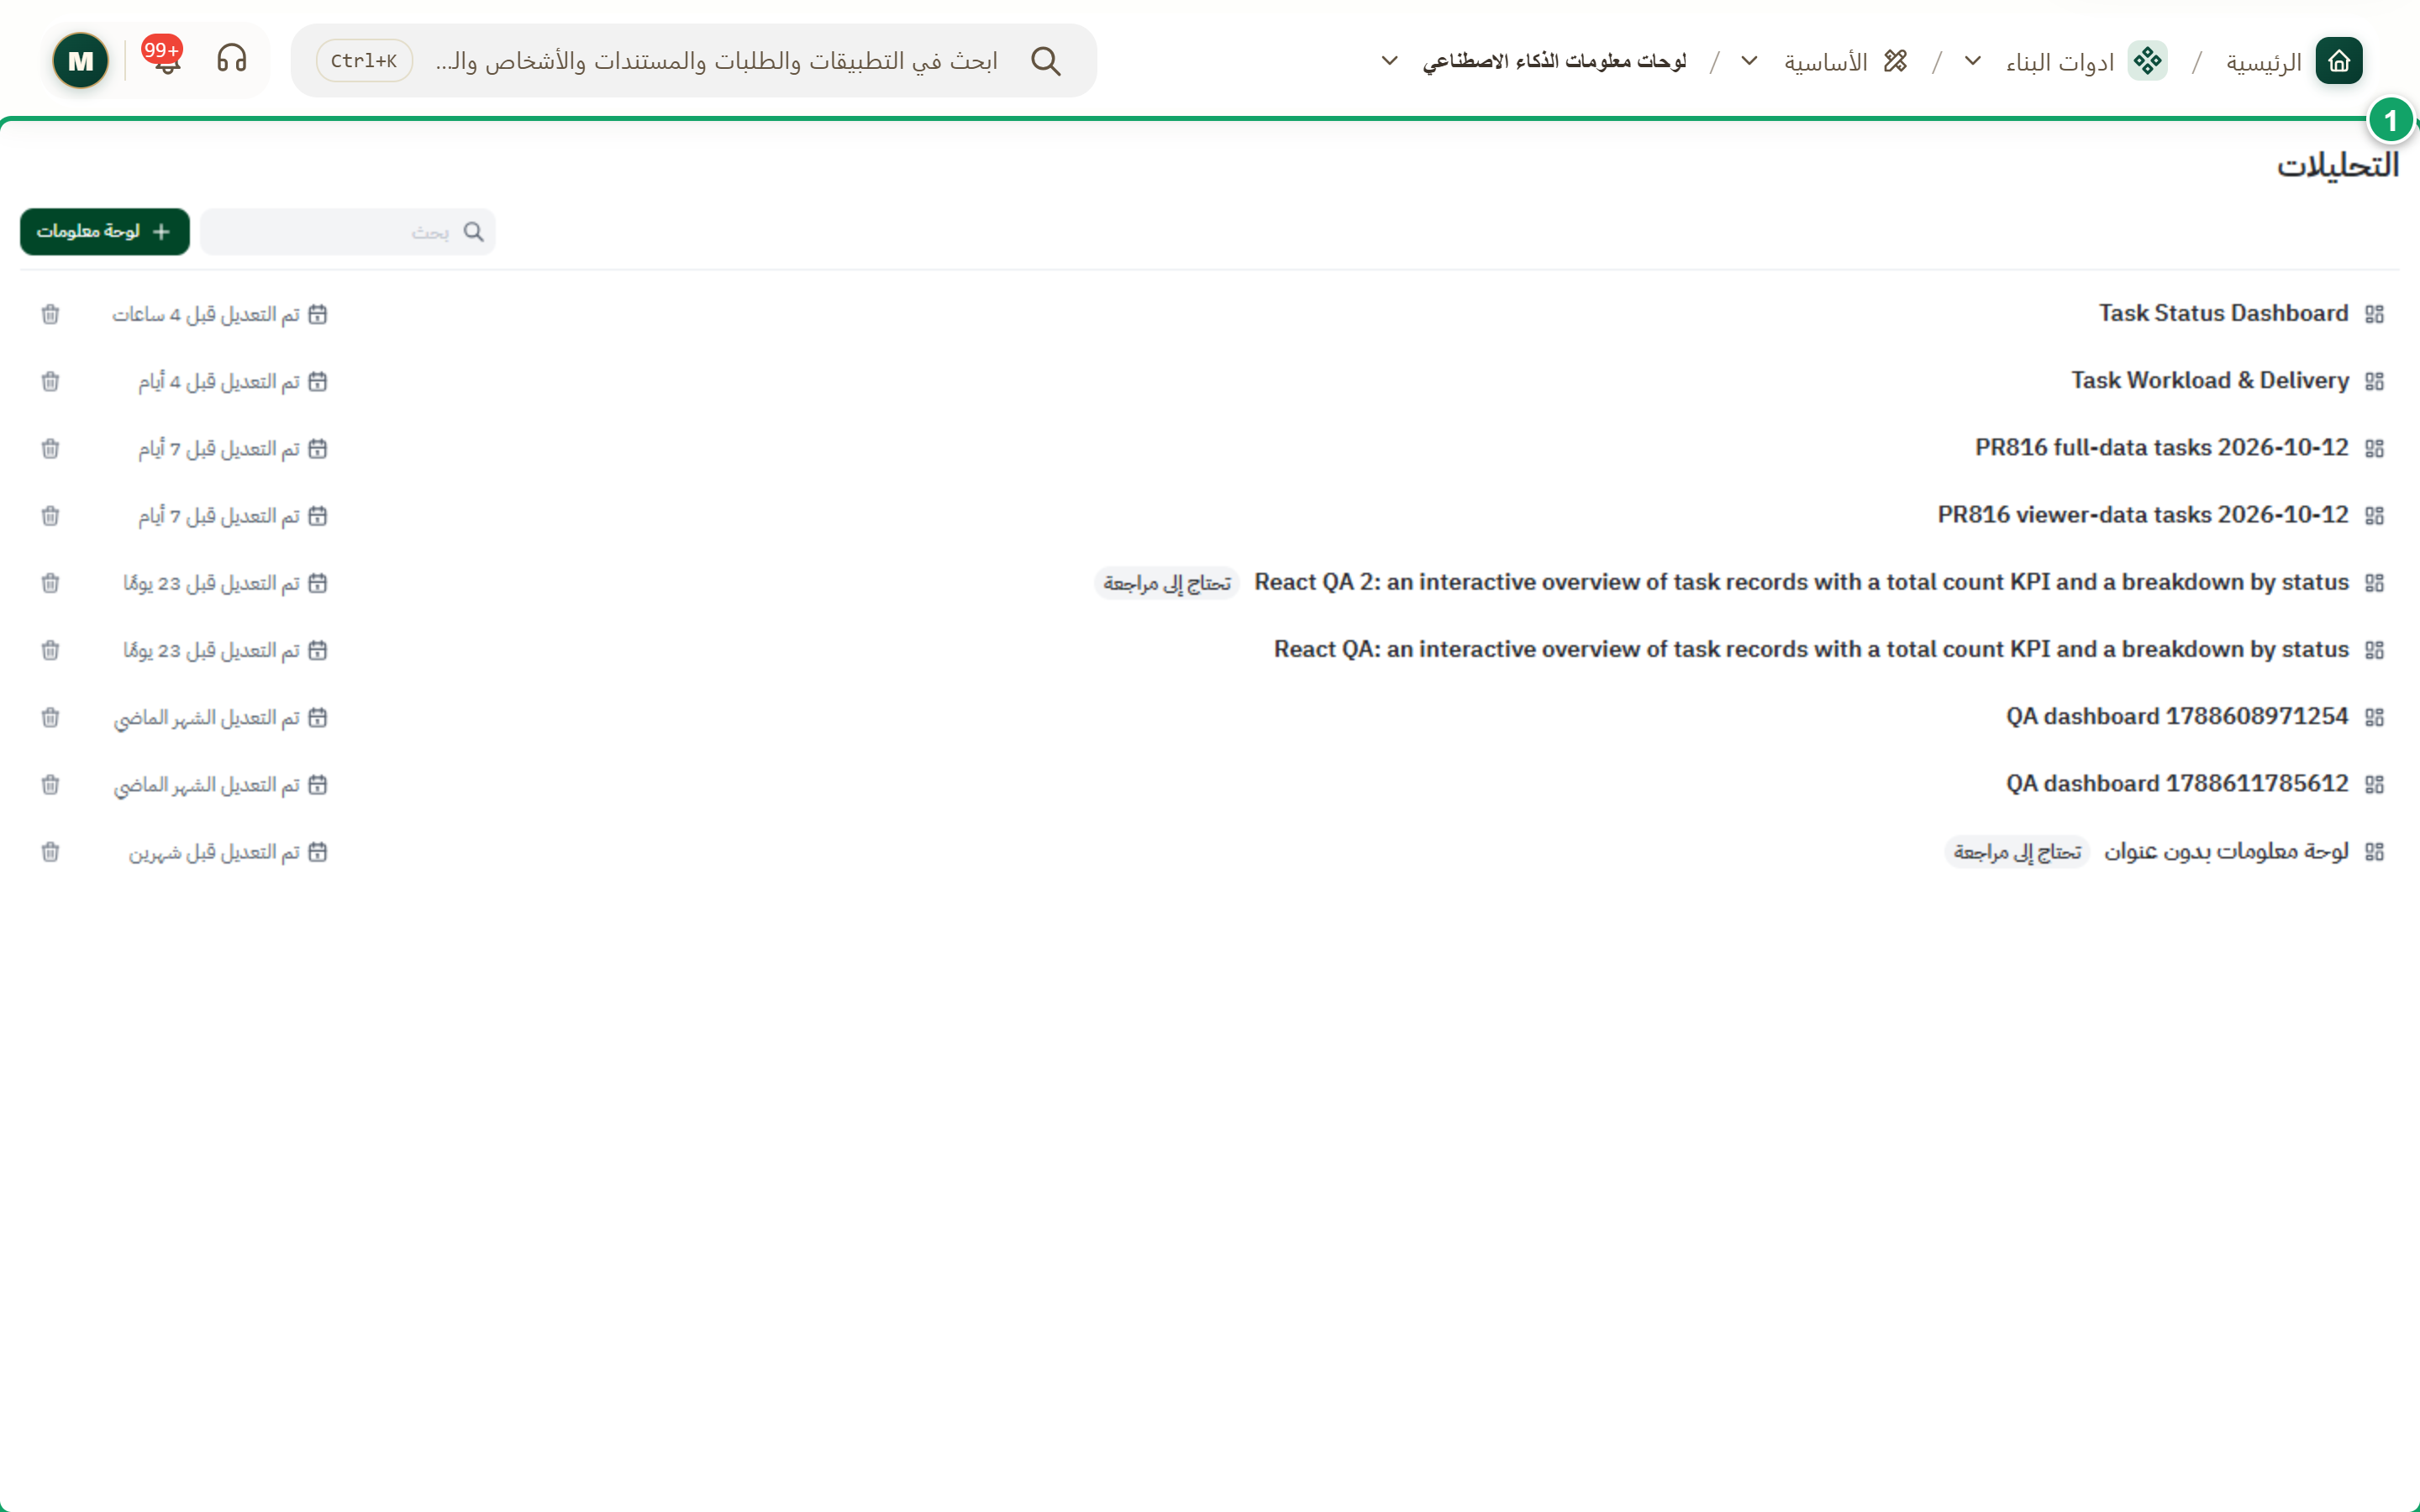
\includegraphics[width=0.95\linewidth,height=0.72\textheight,keepaspectratio]{figures/screens/ch06-ai-dashboards-ar.png}
\caption{مساحة «لوحات معلومات الذكاء الاصطناعي»}
\label{fig:builder-ai-dashboards-screen}
\shotnote{تُفتح مساحة التحليلات داخل كيان، وتعرض لوحات المستخدم الخاصة به. والمحتوى هنا محتوى مؤسسة الاختبار. ① مساحة التحليلات: فيها تُنشأ اللوحات وتُراجَع، ويخدمها نظام التحليلات المضمّن.}
\end{figure}


\begin{table}[H]
\centering
\caption{ما الذي يجب معرفته؟}
\label{tab:builder-ai-dashboards-data}
\begin{tabularx}{\linewidth}{R{3.6cm} Y}
\rcHeaderRow
\thh{الجانب} & \thh{المعنى}\\
مساحة خاصة & اللوحات هنا لك وحدك، وتُحسب من البيانات التي تملك صلاحية قراءتها فقط.\\
بيانات غير متاحة & قد تظهر رسالة بأن بعض البيانات غير متاحة لأن صلاحياتك على أنواع سجلات معينة أوسع من أن تُضمَّن.\\
المشاركة & تُشارك اللوحة بنشرها صفحةً من «الصفحات»، لا من هذه المساحة.\\
\end{tabularx}
\end{table}

\begin{figure}[H]
\centering
\begin{tikzpicture}[node distance=0.5cm]
\node[stepBox] (a) {\RL{وصف ما تريد معرفته}};
\node[stepBox,below=of a] (b) {\RL{مراجعة اللوحة الناتجة}};
\node[stepBox,below=of b] (c) {\RL{نشرها من الصفحات عند الحاجة}};
\draw[flowsTo] (a) -- (b);
\draw[flowsTo] (b) -- (c);
\end{tikzpicture}
\rclegend
\caption{من سؤال إلى لوحة مشتركة}
\label{fig:builder-ai-dashboards-flow}
\shotnote{يضع المخطط المراجعة قبل المشاركة، لأن اللوحة التي يولّدها الذكاء الاصطناعي قد تفهم السؤال على غير ما تقصد. فقارن أرقامها بما تعرفه، ثم شاركها عبر «الصفحات» فقط عندما تثق بها.}
\end{figure}

\subsection{خطوات العمل والتحقق}
\begin{enumerate}
\item افتح «لوحات معلومات الذكاء الاصطناعي»، وانتظر حتى تُحمَّل مساحة التحليلات.
\item أنشئ لوحة جديدة واكتب ما تريد معرفته بوضوح، مع الفترة والحقول المهمة.
\item راجع اللوحة واحفظها، ثم انشرها من «الصفحات» إن أردت أن يراها الفريق.
\end{enumerate}

\textbf{تحقق ومعالجة المشكلة:} يجب أن تُفتح المساحة وتعرض لوحاتك. فإذا ظهرت رسالة «تعذر فتح التحليلات» أو أعادتك الصفحة إلى الرئيسية، فمقعدك لا يتضمن التحليلات أو تنقصك صلاحية عرض لوحات المعلومات؛ فاطلبها من مسؤول المؤسسة.

\clearpage
\section{تقارير الذكاء الاصطناعي}
\label{sec:builder-feature-ai-reports}

تفتح هذه الصفحة مساحة التحليلات نفسها في وضع المحادثة: تسأل بلغتك عن بيانات المؤسسة، فيجيبك الذكاء الاصطناعي بتقرير مكتوب وأرقام. وتناسب الأسئلة السريعة التي لا تحتاج إلى لوحة دائمة، مثل «كم زيارة أُلغيت هذا الشهر ولماذا؟».

\textbf{المسار ومن يستخدمه:} «ادوات البناء» ← «الأساسية» ← «تقارير الذكاء الاصطناعي». شروط ظهورها هي شروط «لوحات معلومات الذكاء الاصطناعي» نفسها.

\begin{rcnote}[مثال: شركة الأفق]
تسأل سارة الخطيب عن الفروع التي تأخرت زياراتها أكثر من أسبوع، فتحصل على تقرير قصير تبني عليه نقاش الاجتماع الشهري. وتطرح سارة سؤالها في المنطقة ①.
\end{rcnote}

\begin{figure}[H]
\centering
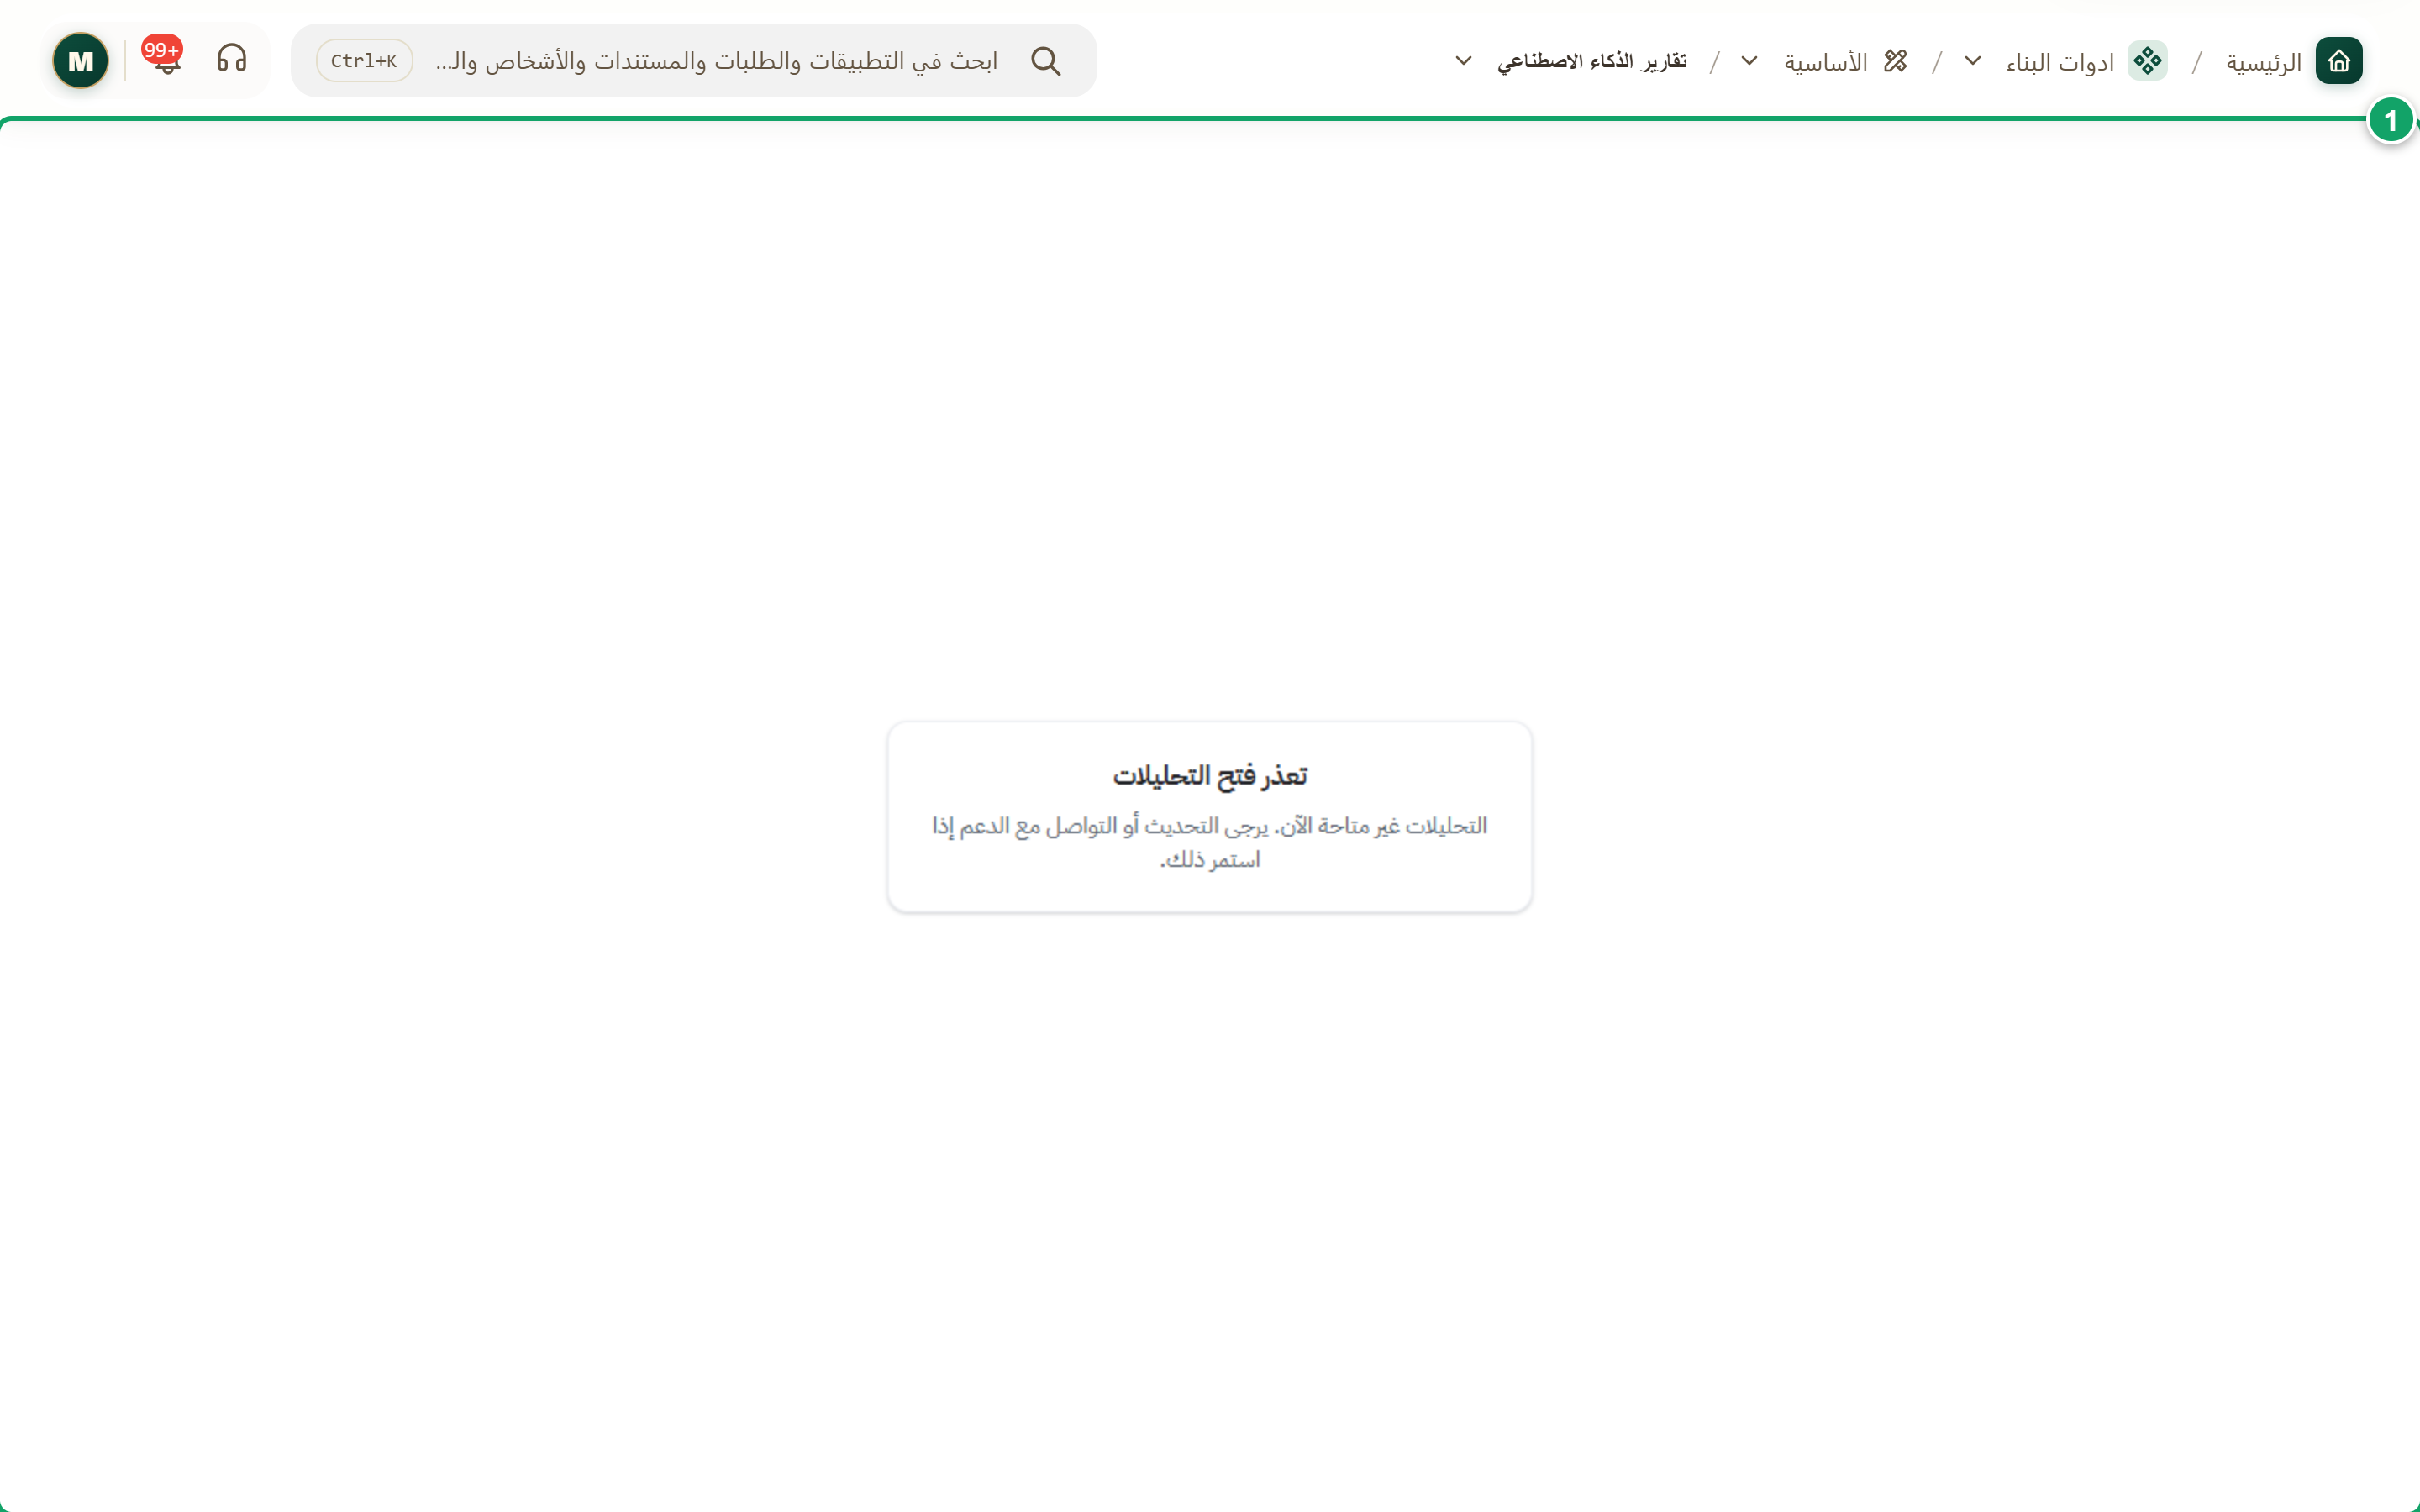
\includegraphics[width=0.95\linewidth,height=0.72\textheight,keepaspectratio]{figures/screens/ch06-ai-reports-ar.png}
\caption{مساحة «تقارير الذكاء الاصطناعي»}
\label{fig:builder-ai-reports-screen}
\shotnote{تُفتح مساحة التحليلات نفسها في وضع المحادثة. ① منطقة المحادثة: تكتب فيها سؤالك وتقرأ التقرير.}
\end{figure}


\begin{table}[H]
\centering
\caption{متى تستخدم التقارير ومتى تستخدم اللوحات؟}
\label{tab:builder-ai-reports-data}
\begin{tabularx}{\linewidth}{R{3.6cm} Y}
\rcHeaderRow
\thh{الحاجة} & \thh{الأنسب}\\
سؤال لمرة واحدة & «تقارير الذكاء الاصطناعي»: اسأل واقرأ الإجابة.\\
متابعة متكررة & «لوحات معلومات الذكاء الاصطناعي» أو «لوحات المعلومات»، لأن اللوحة تُحدَّث وتُراجع دورياً.\\
مشاركة مع الفريق & انشر اللوحة من «الصفحات»؛ فإجابات المحادثة لا تظهر في التنقل.\\
\end{tabularx}
\end{table}

\begin{figure}[H]
\centering
\begin{tikzpicture}[node distance=0.5cm]
\node[stepBox] (a) {\RL{سؤال واضح بفترة محددة}};
\node[stepBox,below=of a] (b) {\RL{قراءة التقرير}};
\node[stepBox,below=of b] (c) {\RL{التحقق من رقم معروف}};
\draw[flowsTo] (a) -- (b);
\draw[flowsTo] (b) -- (c);
\end{tikzpicture}
\rclegend
\caption{طرح سؤال والتحقق من الإجابة}
\label{fig:builder-ai-reports-flow}
\shotnote{ينتهي المخطط بالتحقق، لأن الإجابة مبنية على البيانات التي يستطيع السائل قراءتها وعلى فهم الذكاء الاصطناعي للسؤال. فإذا طابق رقم واحد تعرفه ما في التقرير، زادت ثقتك ببقية الإجابة.}
\end{figure}

\subsection{خطوات العمل والتحقق}
\begin{enumerate}
\item افتح «تقارير الذكاء الاصطناعي»، وانتظر حتى تُحمَّل المحادثة.
\item اكتب سؤالك مع الفترة الزمنية ونوع السجلات المقصود.
\item اقرأ التقرير، وقارن رقماً منه بما تعرفه قبل الاعتماد عليه.
\end{enumerate}

\textbf{تحقق ومعالجة المشكلة:} يجب أن تصل إجابة تشير إلى بيانات مؤسستك. فإذا لم تُفتح الصفحة، فراجع مقعدك وصلاحياتك كما في «لوحات معلومات الذكاء الاصطناعي». وإذا بدت الإجابة ناقصة، فأعد صياغة السؤال بتحديد نوع السجلات والفترة.


\end{document}
